\documentclass[11pt,twoside,openright]{book}
% Preamble for "The Collatz Problem: Martingales, Momentum and Continued Fractions"
% N. G. Polson and V. Sokolov
% House rules: no bold type anywhere, no dashes in prose, no boxed equations.

\usepackage[paperwidth=7in,paperheight=10in,inner=0.875in,outer=0.625in,
  top=0.85in,bottom=0.85in,headsep=0.25in,footskip=0.4in]{geometry}
\usepackage[T1]{fontenc}
\usepackage[utf8]{inputenc}
\usepackage[sc]{mathpazo}
\renewcommand{\ttdefault}{pcr}
\linespread{1.04}
\usepackage{amsmath,amssymb,amsfonts,mathtools}
\usepackage{amsthm}
\usepackage{graphicx,booktabs,array,caption,subcaption,longtable}
\usepackage[numbers,sort&compress]{natbib}
\usepackage{enumitem}
\usepackage{needspace}
\usepackage[expansion=false,protrusion=true]{microtype}
\usepackage{titlesec,fancyhdr,emptypage}
\usepackage[chapter]{algorithm}
\usepackage{algpseudocode}
\usepackage{listings,xcolor}
\usepackage{imakeidx}
\makeindex[intoc,title=Index,columns=2,options=-s collatz.ist]
\usepackage[hidelinks,bookmarksnumbered]{hyperref}
% Generated by bookrepo.py from book.yaml and results.yaml. Edit those files, not this one.
% \BookDOI is empty until zenodo.py reserve; \BookDOIline prints the whole line, or nothing while it is empty (needs hyperref).
% \BookISBN stays empty here: the free KDP ISBN may appear only in the print edition, and kdp.py interior defines it
% for that build alone, so \BookISBNline prints "Paperback ISBN: ..." in print and nothing in the digital edition.
\newcommand*{\BookVersion}{1.1.0}
\newcommand*{\BookEdition}{1}
\newcommand*{\BookYear}{2026}
\newcommand*{\BookDOI}{10.5281/zenodo.23421852}
\newcommand*{\BookDOIline}{Digital Object Identifier (DOI): \href{https://doi.org/10.5281/zenodo.23421852}{\nolinkurl{10.5281/zenodo.23421852}}}
\providecommand*{\BookISBN}{}
\ifx\BookISBN\empty\newcommand*{\BookISBNline}{}\else\newcommand*{\BookISBNline}{Paperback ISBN: \BookISBN}\fi

\usepackage[capitalise,noabbrev]{cleveref}

\numberwithin{equation}{chapter}
\allowdisplaybreaks
\setlength{\parindent}{1.2em}
\setlist{itemsep=2pt,topsep=4pt}

% ---------------------------------------------------------------- headings
\newcommand{\partimagehook}{}
\titleformat{\part}[display]{\centering\normalfont\Large\scshape}
  {\partname\ \thepart}{14pt}{\LARGE\scshape}[\vspace{18pt}\partimagehook]
\titleformat{\chapter}[display]{\normalfont\Large\scshape\filright}
  {\chaptertitlename\ \thechapter}{10pt}{\LARGE\scshape}
\titlespacing*{\chapter}{0pt}{20pt}{28pt}
\titleformat{\section}{\normalfont\large\scshape}{\thesection}{0.8em}{}
\titleformat{\subsection}{\normalfont\normalsize\itshape}{\thesubsection}{0.8em}{}
\titleformat{\subsubsection}[runin]{\normalfont\normalsize\itshape}{}{0pt}{}[.]
\titlespacing*{\section}{0pt}{16pt plus 4pt minus 2pt}{8pt}
\titlespacing*{\subsection}{0pt}{12pt plus 3pt minus 2pt}{6pt}
\renewcommand{\paragraph}[1]{\par\medskip\noindent\textit{#1}\quad}

% ---------------------------------------------------------------- running heads
\pagestyle{fancy}
\fancyhf{}
\renewcommand{\headrulewidth}{0pt}
\renewcommand{\chaptermark}[1]{\markboth{#1}{}}
\renewcommand{\sectionmark}[1]{\markright{#1}}
\fancyhead[LE]{\small\thepage\hfill\itshape On the Collatz Conjecture}
\fancyhead[RO]{\small\itshape\nouppercase{\leftmark}\hfill\upshape\thepage}
\fancypagestyle{plain}{\fancyhf{}\fancyfoot[C]{\small\thepage}}

% ---------------------------------------------------------------- captions
\captionsetup{font=small,labelfont=sc,labelsep=period,width=0.95\textwidth}
\DeclareCaptionStyle{ruled}{font=small,labelfont=sc,labelsep=period,strut=off}

% ---------------------------------------------------------------- theorems
% amsthm in place of thmtools: thmtools v0.76 raises "Command \c@proposition
% already defined" for shared counters under the TeX Live 2026 kernel.
% Same styles and numbering as the original \declaretheorem block.
\newtheoremstyle{thmstyle}{8pt plus 2pt}{8pt plus 2pt}{\itshape}{0pt}
  {\normalfont\scshape}{.}{0.5em}
  {\thmname{#1}\thmnumber{ #2}\thmnote{ {\normalfont\itshape(#3)}}}
\newtheoremstyle{defstyle}{8pt plus 2pt}{8pt plus 2pt}{\normalfont}{0pt}
  {\normalfont\scshape}{.}{0.5em}
  {\thmname{#1}\thmnumber{ #2}\thmnote{ {\normalfont\itshape(#3)}}}
\theoremstyle{thmstyle}
\newtheorem{theorem}{Theorem}[chapter]
\newtheorem{proposition}[theorem]{Proposition}
\newtheorem{lemma}[theorem]{Lemma}
\newtheorem{corollary}[theorem]{Corollary}
\newtheorem{conjecture}[theorem]{Conjecture}
\theoremstyle{defstyle}
\newtheorem{definition}[theorem]{Definition}
\newtheorem{example}[theorem]{Example}
\newtheorem{remark}[theorem]{Remark}
\newtheorem*{problem*}{Problem}
% \designation{O2}\label{prob:ch11:o2} in an unnumbered problem: \ref prints the designation O2 (\cref would print the enclosing section)
\makeatletter
\newcommand{\designation}[1]{\phantomsection\def\@currentlabel{#1}}
\makeatother
\newtheorem{exercise}[theorem]{Exercise}
\crefname{conjecture}{Conjecture}{Conjectures}
\crefname{exercise}{Exercise}{Exercises}
\renewcommand{\qedsymbol}{$\square$}
\renewcommand{\proofname}{\textit{Proof}}

% ---------------------------------------------------------------- algorithms
\algrenewcommand\algorithmicrequire{\textit{Input:}}
\algrenewcommand\algorithmicensure{\textit{Output:}}
\algrenewcommand\algorithmicfor{\textit{for}}
\algrenewcommand\algorithmicdo{\textit{do}}
\algrenewcommand\algorithmicif{\textit{if}}
\algrenewcommand\algorithmicthen{\textit{then}}
\algrenewcommand\algorithmicelse{\textit{else}}
\algrenewcommand\algorithmicend{\textit{end}}
% line anchors unique across algorithms (numbered by chapter)
\makeatletter
\providecommand*{\theHALG@line}{}
\renewcommand*{\theHALG@line}{\thealgorithm.\arabic{ALG@line}}
% index page ranges are printed with " to " (collatz.ist); link both ends
\let\collatz@hyperpage\hyperpage
\renewcommand*{\hyperpage}[1]{\collatz@hpsplit#1 to \@nil}
\def\collatz@hpsplit#1 to #2\@nil{%
  \if\relax\detokenize{#2}\relax\collatz@hyperpage{#1}%
  \else\collatz@hprange{#1}#2\@nil\fi}
\def\collatz@hprange#1#2 to \@nil{\collatz@hyperpage{#1} to \collatz@hyperpage{#2}}
\makeatother
\algrenewcommand\algorithmicreturn{\textit{return}}
\makeatletter
\renewcommand\fs@ruled{\def\@fs@cfont{\scshape}\let\@fs@capt\floatc@ruled
  \def\@fs@pre{\hrule height.8pt depth0pt \kern2pt}%
  \def\@fs@post{\kern2pt\hrule\relax}%
  \def\@fs@mid{\kern2pt\hrule\kern2pt}\let\@fs@iftopcapt\iftrue}
\makeatother

% ---------------------------------------------------------------- code
\lstset{basicstyle=\ttfamily\footnotesize,keywordstyle=\ttfamily,columns=fullflexible,keepspaces=true,
  frame=lines,framesep=4pt,xleftmargin=6pt,xrightmargin=6pt,
  commentstyle=\itshape\color{black!60},showstringspaces=false,
  breaklines=true,language=Python}

% ---------------------------------------------------------------- macros
\newcommand{\N}{\mathbb{N}}
\newcommand{\Z}{\mathbb{Z}}
\newcommand{\Q}{\mathbb{Q}}
\newcommand{\R}{\mathbb{R}}
\newcommand{\E}{\mathbb{E}}
\newcommand{\Prob}{\mathbb{P}}
\newcommand{\Var}{\operatorname{Var}}
\newcommand{\Cov}{\operatorname{Cov}}
\newcommand{\KL}{D_{\mathrm{KL}}}
\newcommand{\vt}{v_2}
\newcommand{\ds}{\delta^{*}}
\newcommand{\half}{\tfrac{1}{2}}
\newcommand{\Filt}{\mathcal{F}}
\newcommand{\Ztwo}{\mathbb{Z}_2}
\newcommand{\lt}{\log_2 3}
\newcommand{\wt}{\operatorname{wt}}
\newcommand{\off}{\operatorname{off}}
\newcommand{\src}{\operatorname{src}}
\newcommand{\smmdet}{\ensuremath{\mathrm{SMM}_{\mathrm{det}}}}
\newcommand{\smmstate}{\ensuremath{\mathrm{SMM}_{\mathrm{state}}}}

% table of contents without bold
\usepackage{etoolbox}
\makeatletter
\patchcmd{\l@chapter}{\bfseries}{\scshape}{}{}
\patchcmd{\l@part}{\bfseries}{\scshape}{}{}
\makeatother

% no line break hyphenation (house style), with stretch to compensate
\hyphenpenalty=10000
\exhyphenpenalty=10000
\setlength{\emergencystretch}{3em}


\begin{document}

\frontmatter
% Half title, title page, copyright page, dedication
\thispagestyle{empty}
\begin{center}
\vspace*{2.2in}
{\Huge\scshape On the Collatz Conjecture}
\end{center}
\cleardoublepage

\thispagestyle{empty}
\begin{center}
\vspace*{1.1in}
{\huge\scshape On the Collatz Conjecture}\\[16pt]
{\Large\itshape Martingales, Momentum\\[4pt] and Continued Fractions}\\[1.2in]
{\Large Nick Polson}\\[4pt]
{\small Booth School of Business, University of Chicago}\\[22pt]
{\Large Vadim Sokolov}\\[4pt]
{\small George Mason University}
\vfill
{\small 2026}
\end{center}
\clearpage

\thispagestyle{empty}
\vspace*{\fill}
{\small\noindent
Copyright \copyright\ 2026 Nicholas G.\ Polson and Vadim Sokolov.\\[8pt]
On the Collatz Conjecture: Martingales, Momentum and Continued Fractions.\\[8pt]
Mathematics Subject Classification (2020): 11B83, 11J70, 37P99, 60G42, 90C25.\\[8pt]
Every number computed in this book comes from code that accompanies it, and the scripts are listed in \cref{app:code}; numbers quoted from the literature are cited where they appear.
The source, the code and the digital edition are at \url{https://github.com/VadimSokolov/collatz}, and the book's page is \url{https://vsokolov.org/books/collatz/}.
The figures are in colour in the digital edition and in grayscale in the paperback.
The text was typeset in \LaTeX\ with
the Palatino typeface.\\[8pt]
First edition, October 2026.%
\ifx\BookISBNline\empty\else\\[8pt]\BookISBNline\fi
\ifx\BookDOIline\empty\else\\[8pt]\BookDOIline\fi
\\[8pt]License: distributed under the Creative Commons Attribution 4.0 International License (CC BY 4.0), \url{https://creativecommons.org/licenses/by/4.0/}: you may copy, share and adapt this book for any purpose, provided you credit the authors. The code is released under the MIT License.\\[8pt]
Independently published.\par}
\cleardoublepage

\thispagestyle{empty}
\vspace*{2in}
\begin{center}
\itshape
For the students who keep computing the orbit of $27$.
\end{center}
\cleardoublepage

\tableofcontents
\chapter*{Preface}
\addcontentsline{toc}{chapter}{Preface}
\markboth{Preface}{Preface}

Take a positive integer. If it is even, halve it; if it is odd, triple it and
add one. Repeat. The Collatz conjecture says that every starting value
eventually reaches $1$. It can be explained to a child in a minute, checked by
a laptop for every number a person could write down in a lifetime, and it has
resisted every serious attempt at proof since the 1930s. This book is about
why.

We came to the problem from outside number theory. One of us works in Bayesian
statistics and probability, the other in optimization and machine learning,
and what drew us in was a simple observation that anyone trained in either
field makes within an hour of looking at the map. The logarithm of the iterate
behaves like a random walk with negative drift. Each odd step multiplies by
about $3/2$, each even step divides by $2$, and if the parities were fair coin
flips the expected change in $\log x$ per step would be
$\tfrac12\log\tfrac32-\tfrac12\log2=\log(\sqrt3/2)\approx-0.144$. That is a
Lyapunov function decreasing in expectation, the most familiar object in
optimization and control, and it predicts the growth of the stopping times of
real orbits to within about two percent. None of it is a proof, and the reason it is not a
proof is the subject of the book.

\section*{What the book does}

We read the Collatz dynamics as an optimization problem and push the reading
as far as it will go. Three things come out.

The first is an accounting of what a proof would have to contain. The
conjecture splits into two halves that require completely different tools.
The divergence half asks whether $\log x_n$ can drift upward forever along a
single orbit.
It is equivalent to a statement about Ces\`aro averages of the dyadic valuations $\vt(3y+1)$ along that orbit, namely that the lower limit of their running mean exceeds $\log_2 3\approx1.585$ (\cref{conj:cesaro}), and it is a one sided law of large numbers for a deterministic sequence that nobody knows how to prove.
The cycle half asks
whether an orbit can close up. It is not an averaging question at all: a cycle
forces a product of numbers slightly larger than $3$ to equal a power of $2$,
so the rational approximations of $\log_2 3$ enter, although, as we show, they cannot decide it on their own.

The second is a set of structural theorems, most of them short and several of
them classical. We prove that the Syracuse
exponent is exactly Geometric$(\tfrac12)$ on residue classes, that under the
Bernoulli model the iterates form a multiplicative martingale while their
logarithms form a strict supermartingale (the gap between the two is Jensen's
inequality), that the parity autocorrelation function of the standard map is
$\rho(h)=(-\tfrac12)^h$ in the model, and that no monotone Lyapunov function certifies descent over any
fixed number of strides. On cycles we give a short mediant lemma for the one sided distances $\lceil r\log_23\rceil-r\log_23$ which, with a self contained proof of the classical description of the one sided best approximations, shows that only the upper rungs of the semiconvergent ladder of $\log_23$ ever need to be checked. Combined with verification up to $2^{68}$ it gives, unconditionally,
that every nontrivial cycle has at least $72\,057\,431\,991$ odd elements. The
method goes back to Crandall and Eliahou, the bound is that of Hercher and
Puchert, and we claim no priority for any numerical bound; the current record,
$r\geq1.375\times10^{11}$, is Hercher's, made unconditional by Ba\v{r}ina's
verification to $2^{71}$. What we offer is a short rigorous route to the bound
and an exact integer certificate for it. We then prove that Diophantine
information about $\log_23$ alone cannot finish the cycle half, since infinitely many cycle lengths survive
every verification range, and we show with a window lemma that an arithmetic
improvement of the basic cycle inequality by a factor slightly larger than $r/3$, combined with a finite verification, would.
On the computational side, nested, split and vertical likelihood sampling reach regions of exponentially small prior mass in a number of steps polynomial in the depth, provided each level set can be sampled exactly. We prove that a perfect version of split sampling samples the exceptional residue classes exactly, at any depth and in time polynomial in the depth. Beyond the bit length of the integers the level set samplers eventually stop, and for split sampling the census shows why: in the boxes we computed, the slow integers are a small number of long orbits together with their tributaries, and a local sampler leaves the tree it starts in only about as often as rejection sampling finds a new one.

The third is an algorithm. The Collatz map alternates an ascent, the odd step,
with a corrective descent, the run of halvings, and the ratio of the two
logarithmic step sizes is $\beta=\log(3/2)/\log2=\log_23-1\approx0.585$. We
turn this into Switching MM, a first order method with fixed momentum $\beta$
that extrapolates only on odd iterations. On quadratics we prove that two of
its steps are exactly a gradient step of size $\alpha$ followed by one of size
$(1+\beta)\alpha$, so that it is a cyclic step size method in disguise, and we
compute its stationary variance under gradient noise in closed form. The
noise amplification of Switching MM relative to gradient descent at the same step is bounded by $5/3$ for every $\beta<1$,
whereas in the slow modes every step momentum amplifies noise by $1/(1-\beta)$, which is $10$ at
the machine learning default $\beta=0.9$. That is the precise sense in which
the parity schedule is a low tuning default. For any smooth strongly convex
function we prove a linear rate whose factor is the exact worst case for the distance to the minimizer, and a gain weight theorem shows that no periodic
momentum schedule of any period can beat gradient descent's noise floor in the slow modes at
matched speed: momentum trades speed for noise in exact proportion, and unequal
weighting of gradients pays a Cauchy and Schwarz penalty.

\section*{What the book does not do}

It does not prove the Collatz conjecture. We say this at the outset and repeat
it where it matters, because the literature on the problem contains many
claimed proofs and the optimization language makes it easy to mistake a
heuristic for an argument. Several of the most instructive passages in the
book are pitfalls: arguments that look like progress and are not. The Ces\`aro
criterion $\bar k_N>\log_23$ holds automatically at the stride $N$ at which an orbit reaches $1$,
so checking it numerically on terminating orbits carries no information. Convergent
denominators alone do not locate the records of the cycle bound, because the
relevant distance is one sided. In the stochastic model, the linear majorizer of the logarithm has positive mean increment while the logarithm itself has negative drift.
Two constants near one half, a momentum rate that pairs an ascent and a descent measured at different levels and the modulus of an eigenvalue of a chain conditioned on a set that it leaves, agree by accident (\cref{rem:ch5:mixing}).

\section*{How to read it}

Part I sets up the problem: the history and the three standard maps (\cref{chap:intro}), the arithmetic of parity vectors and the Syracuse map including Terras' theorem and the density result (\cref{chap:parity}), and the stochastic models with their martingales (\cref{chap:stochastic}). Part II is the optimization reading: Lyapunov functions and their limits (\cref{chap:lyapunov}); majorization and momentum (\cref{chap:momentum}); majorization pressed to its limit on the Collatz map, where it reproduces the cycle inequality and shows that no correction of $\log x$ by a function of the last $d$ binary digits of $x$, for any fixed $d$, certifies descent (\cref{chap:mmcollatz}); Switching MM as an optimizer (\cref{chap:smm}) and its behaviour under noise, with experiments (\cref{chap:noise}); nonlinear difference equations and momentum MM, with difference inequalities for the inverse tree and a linear rate for Switching MM on smooth strongly convex functions that is tight for the distance to the minimizer (\cref{chap:difference}); and the three point inequalities and similar triangles behind every convergence proof, which give Switching MM a convex rate a factor $1+\beta/2$ better than gradient descent and show what the Collatz map lacks (\cref{chap:threepoint}). Part III treats cycles through continued fractions, with a section on the sibling problem of Erd\H{o}s $125$ settled by machine checked proof search and on our own Lean statements (\cref{chap:cycles}); the divergence half through Ces\`aro averages, mixing and Tao's theorem (\cref{chap:divergence}); the positive density theorems of 2026, read as the stride model run backwards through the inverse tree, with numerical checks of their constants and of the $3$ adic law they rest on (\cref{chap:backward}); a synthesis of what a proof would require (\cref{chap:path}); a computational path, with what the MM view implies for automated certificates (\cref{chap:computation}); what nested, split and vertical likelihood sampling can and cannot do, with the tree structure of the slow integers (\cref{chap:samplers}); progress on six of the open problems, including the third cumulant of stopping times and the exact convex rate of Switching MM (\cref{chap:progress}); a summary of what the book contributes, a ledger of the strategies it rules out, and a computational road map to a solution (\cref{chap:synthesis}); and a list of open problems and computational projects (\cref{chap:open}). A gallery of computed pictures follows Part III, and two appendices tabulate the constants and describe the code.

A reader interested only in the optimizer can read \cref{chap:momentum,chap:smm,chap:noise} and then \cref{chap:difference,chap:threepoint}, which use their results, turning back to Part I and \cref{chap:lyapunov} for the stride arithmetic behind the momentum constant. A reader interested only in the number theory can go from Part I directly to \cref{chap:cycles,chap:divergence}, but before \cref{chap:path,chap:computation} needs the impossibility results of \cref{chap:lyapunov,chap:mmcollatz} and the first two sections of \cref{chap:difference} (with \cref{sec:ch5b:stability} for two comparisons in \cref{chap:computation}). Every chapter ends with notes, and every chapter except \cref{chap:open} with exercises.

\section*{Acknowledgements}

We thank participants at the Chicago Booth Statistics Workshop and colleagues
who listened to early versions of these arguments and pointed out the ones
that were wrong. The computations were done in Python with mpmath, NumPy,
SciPy, SymPy, Numba, CVXPY and scikit-learn, and the figures were drawn with Matplotlib; the formal statements in \cref{chap:cycles} were checked in
Lean~4.

\vspace{12pt}
\noindent Chicago and Fairfax, October 2026\hfill N.\,G.\,P.\quad V.\,S.

\chapter*{Notation}
\addcontentsline{toc}{chapter}{Notation}
\markboth{Notation}{Notation}

The table lists the symbols that a reader meets in more than one chapter, or that a later chapter uses without redefining. When a letter carries different meanings in different parts of the book, its row says so. Symbols local to one proof or one section are defined where they occur.

\begingroup
\linespread{1}\footnotesize
\setlength{\tabcolsep}{4pt}
\begin{longtable}{@{}>{\raggedright\arraybackslash}p{0.95in}>{\raggedright\arraybackslash}p{3.3in}>{\raggedright\arraybackslash}p{1.0in}@{}}
\toprule
Symbol & Meaning & Defined in \\
\midrule
\endfirsthead
\toprule
Symbol & Meaning & Defined in \\
\midrule
\endhead
\bottomrule
\endfoot
$T_0$, $T_0^{(k)}$ & standard map, $n/2$ for even $n$ and $3n+1$ for odd $n$, and its $k$th iterate & \cref{def:maps} \\
$T$, $T^{(k)}$ & accelerated map, $n/2$ for even $n$ and $(3n+1)/2$ for odd $n$, and its $k$th iterate & \cref{def:maps} \\
$S$, $S^{(k)}$ & Syracuse map on odd $n$, $S(n)=(3n+1)/2^{\vt(3n+1)}$, and its $k$th iterate; one step of $S$ is a stride & \cref{def:maps} \\
$\vt(m)$ & the $2$ adic valuation: the exponent of the largest power of $2$ dividing $m\neq0$ & \cref{def:maps} \\
$k$, $k_j$, $\bar k_N$ & halving exponent $\vt(3x+1)$ of the stride from an odd $x$; $\bar k_N$ is the mean of $k_1,\dots,k_N$ along an orbit of $S$ & \cref{sec:ch2:maps}, \cref{chap:divergence} \\
$v_k(n)$, $m_k(n)$, $\Phi_k$ & parity vector of $n$ under $T$ (first $k$ steps), its number of ones (the odd steps), and the Terras bijection $n\bmod2^k\mapsto v_k(n)$ of residue classes onto parity vectors & \cref{def:ch2:parity}, \cref{thm:terras} \\
$c_k(n)$ & the integer in $2^kT^{(k)}(n)=3^{m_k(n)}n+c_k(n)$, determined by $v_k(n)$ & \cref{prop:ch2:affine} \\
$\Ztwo$, $\mu$, $E$ & the $2$ adic integers, their Haar probability measure $\mu$, and the closed null set $E$ of points with infinite coefficient stopping time & \cref{sec:ch2:adic}, \cref{sec:ch10b:divergence} \\
\addlinespace[4pt]
$\sigma(n)$ & stopping time: least $k\geq1$ with $T^{(k)}(n)<n$; unrelated to the standard deviation $\sigma$ below & \cref{def:ch2:stopping} \\
$\sigma_\infty(n)$ & total stopping time: least $k$ with $T_0^{(k)}(n)=1$ in \cref{chap:intro}, but with $T^{(k)}(n)=1$ in \cref{chap:stochastic,chap:samplers,chap:open} & \cref{sec:ch1:conjecture} \\
$\tau(n)$ & coefficient stopping time: least $k\geq1$ with $3^{m_k(n)}<2^k$; in \cref{chap:stochastic,chap:lyapunov}, $\tau$ is instead a first passage time of a model walk & \cref{def:ch2:stopping} \\
\addlinespace[4pt]
Bernoulli, stride and renewal models & coin models of $T$ (factors $\xi_i\in\{\frac12,\frac32\}$), of $S$ (factors $3\cdot2^{-K_j}$) and of $T_0$ (parity chain $B_n$) & \cref{def:ch3:models} \\
$\ds$, $\log\frac34$ & model drift of $\log x$: $\ds=\log(\sqrt3/2)$ per step of $T$, $\log\frac34$ per stride of $S$, $\frac13\log\frac34$ per step of $T_0$; $\ds$ is not $\delta(r)$ & \cref{thm:martingale,cor:ch2:drift,prop:ch3:standard} \\
$\sigma^2$, $C$, $\gamma_0$ & variance $\frac14(\log3)^2$ of a log step of $T$, index of dispersion $C=\sigma^2/(\ds)^2\approx14.58$, and slope $\gamma_0=1/|\ds|\approx6.95$ of the model total stopping time of $T$ in $\log n$; in \cref{chap:noise}, $\sigma^2$ is the gradient noise variance & \cref{prop:lyapunov}, \cref{sec:ch7:model} \\
\addlinespace[4pt]
$\lt$, $\theta$ & $\lt=1.58496\dots$ is the Ces\`aro threshold for $\bar k_N$; $\theta$ is $\lt$ in \cref{chap:cycles}, $1/\lt$ in \cref{thm:density}, and an exponent in \cref{thm:martingale} & \cref{sec:ch1:conjecture}, \cref{chap:cycles} \\
$r$, $s$, $M$, $\Lambda$ & cycle of $S$: $r$ odd elements, $s$ halvings (one turn is $r$ steps of $S$, $s$ of $T$, $r+s$ of $T_0$), least element $M$, $\Lambda=s\log2-r\log3$; written $m$, $k$ in \cref{chap:parity,chap:open} & \cref{lem:cycleid}, \cref{rem:ch8:bookkeeping} \\
$\delta(r)$, $\Lambda_r$, $F(r)$ & $\delta(r)=\lceil r\theta\rceil-r\theta$, $\Lambda_r=\delta(r)\log2\le\Lambda$, $F(r)=r/(3\Lambda_r)>M$ & \cref{eq:ch8:Lambdar}, \cref{eq:ch8:maxM} \\
$a_k$, $p_k/q_k$, $u_{k,j}$ & partial quotients, convergents $1,2,\frac32,\frac85,\frac{19}{12},\dots$ and ladder rungs $q_{k-1}+jq_k$ of $\lt=[1;1,1,2,2,3,\dots]$ & \cref{sec:ch8:cf}, \cref{tab:ch8:conv} \\
$\nu_k$ & irrationality exponent $-\log|\theta-p_k/q_k|/\log q_k$ of the $k$th convergent; unrelated to $\nu_1,\nu_2$ in \cref{sec:ch7:multiplicative} & \cref{sec:ch8:limits} \\
$X$ & verified range: every nontrivial cycle has all its elements at least $X$; $X=2^{71}$ is established & \cref{def:ch8:excl} \\
\addlinespace[4pt]
$V$ & Lyapunov function (certificate), the standard potential being $V(x)=\log x$; in \cref{chap:noise}, $V_{\mathrm{GD}}$, $V_{\mathrm{SMM}}$ and $V(\beta)$ are variances & \cref{def:ch4:lyap} \\
$\varphi$, $G_d$ & residue correction in the potential $V(x)=\log x+\varphi(x\bmod2^d)$, and the residue graph with edge weights $\log\frac32$ (odd) and $-\log2$ (even) & \cref{sec:ch5c:residue}, \cref{thm:ch5c:residue} \\
\addlinespace[4pt]
$\mu$, $L$, $\kappa$, $\lambda$, $e_t$ & $f$ is $\mu$ strongly convex with $L$ Lipschitz gradient and $\kappa=L/\mu$ is its condition number; $\lambda$ is a Hessian eigenvalue and $e_t=x_t-x^\ast$ the error; $\mu$ is also the Haar measure, and $L$ an energy in \cref{chap:samplers} & \cref{sec:ch5:momentum} \\
$L$, $\mu$, $\kappa$ (stride) & stride constants of \cref{chap:momentum}: $L=\log\frac53$ the largest ascent, $\mu=|\log\frac34|$ the mean descent, $\kappa=L/\mu\approx1.776$ a ratio of increments and not a condition number & \cref{def:nesterov} \\
$\alpha$, $a$, $\beta$ & step size, usually $1/L$; the normalized step $a=\alpha\lambda$; momentum coefficient $\beta$, equal to $\log(3/2)/\log2=\lt-1$ in SMM; in \cref{chap:samplers}, $\beta$ is an inverse temperature & \cref{sec:ch6:problem}, \cref{sec:ch5:beta} \\
\smmdet, \smmstate, $G_h$ & Switching MM: \smmdet\ extrapolates on odd iterations only, two steps from an even index being $G_{(1+\beta)\alpha}\circ G_\alpha$ with $G_h(x)=x-h\nabla f(x)$; \smmstate\ injects only when progress is slow & \cref{alg:smmdet}, \cref{thm:smmquad} \\
$m_{\mathrm{SMM}}$, $V(\beta)$ & slow mode step multiplier $(2+\beta)/2$ and noise amplification $(2+2\beta+\beta^2)/(2+\beta)$ of \smmdet & \cref{cor:ch6:slow}, \cref{eq:ch7:V} \\
\end{longtable}
\endgroup


\mainmatter

\renewcommand{\partimagehook}{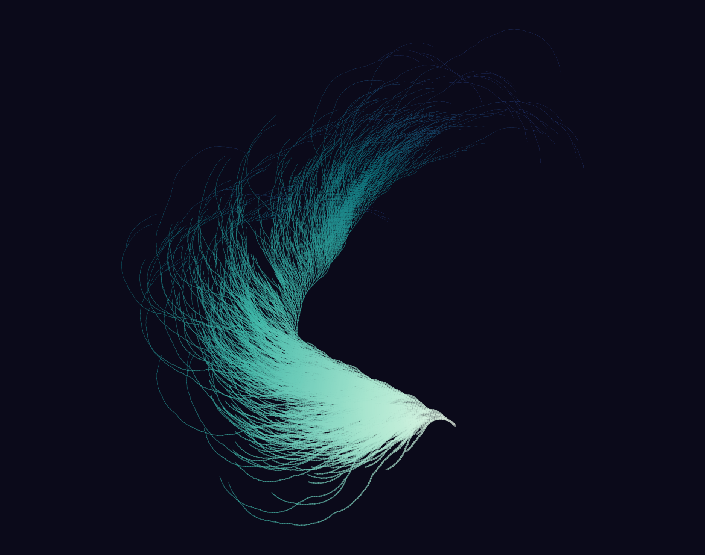
\includegraphics[width=1\textwidth]{figures/art_part1}\par\vspace{8pt}{\normalsize\upshape\itshape The Collatz coral: the orbits of the first $20\,000$ integers, drawn from $1$ outward with a small turn at every step, one way at even values and the other at odd values; colour is total stopping time.\par}}
\part{The Problem}
\chapter{The $3x+1$ Problem}\label{chap:intro}

Take a positive integer. If it is even, halve it; if it is odd, triple it and
add one. Repeat. Starting from $7$ the sequence runs
\[
  7,\ 22,\ 11,\ 34,\ 17,\ 52,\ 26,\ 13,\ 40,\ 20,\ 10,\ 5,\ 16,\ 8,\ 4,\ 2,\ 1,
\]
and once it reaches $1$ it falls into the loop $1\to4\to2\to1$ forever. The
$3x+1$ problem asks whether this always happens. Every starting value that
anyone has ever tried, and the number of starting values tried is now
$2^{71}$, eventually reaches $1$. Nobody knows why.

The problem can be explained to a child and has defeated some of the strongest
mathematicians of the last ninety years. It sits at an unusual junction. The
rule is arithmetic, but the behaviour it produces looks random; the obvious
probabilistic heuristic predicts the answer with great accuracy, but the
heuristic is not a proof and no one knows how to turn it into one; and
generalizations of the problem that look only slightly more complicated are
provably undecidable. This book is about that junction, read through the lens
of martingales\index{martingale}, optimization and Diophantine\index{Diophantine approximation} approximation. This first chapter
states the problem, recounts its history, works through examples, surveys what
is known, and lays out the plan of the book.

\section{The conjecture}\label{sec:ch1:conjecture}

We write $\N=\{1,2,3,\ldots\}$ for the positive integers. The \emph{standard
Collatz map} $T_0:\N\to\N$ is
\begin{equation}\label{eq:ch1:T0}
  T_0(n)=\begin{cases} n/2, & n \text{ even},\\ 3n+1, & n \text{ odd}.\end{cases}
\end{equation}
We write $T_0^{(k)}$ for the $k$th iterate, with $T_0^{(0)}(n)=n$, and call the
sequence $n, T_0(n), T_0^{(2)}(n),\ldots$ the \emph{orbit} or
\emph{trajectory} of $n$.

\begin{conjecture}[The Collatz conjecture]\label{conj:ch1:collatz}
For every $n\in\N$ there is $k\geq0$ with $T_0^{(k)}(n)=1$.
\end{conjecture}

The least such $k$ is the \emph{total stopping time\index{stopping time}} of $n$, written
$\sigma_\infty(n)$, with the convention $\sigma_\infty(n)=\infty$ if no such
$k$ exists. The conjecture says $\sigma_\infty(n)<\infty$ for every $n$.

It is useful to see at once what could go wrong. The orbit of $n$ is a sequence
of positive integers, so exactly one of three things happens.
\begin{enumerate}[label=(\roman*),leftmargin=2em]
\item The orbit reaches $1$, and from then on cycles through $1,4,2$.
\item The orbit is unbounded: $\limsup_k T_0^{(k)}(n)=\infty$. Since the orbit
  cannot revisit a value without becoming periodic, in this case all its
  values are distinct and in fact $T_0^{(k)}(n)\to\infty$.
\item The orbit is bounded but never reaches $1$. A bounded orbit takes only
  finitely many values, so it must eventually repeat a value, and then it is
  periodic from that point on. Hence the orbit enters a cycle that does not
  contain $1$.
\end{enumerate}
The conjecture is the assertion that alternatives (ii) and (iii) never occur.
We shall call these the \emph{divergence half} and the \emph{cycle half} of
the problem. They look like two aspects of one question, but one of the main
messages of this book is that they are different in kind and call for
different tools.

That the problem is genuinely arithmetic, and not a consequence of some soft
principle about tripling and halving, is shown by running the same rule on the
negative integers\index{negative cycles}. Formula \eqref{eq:ch1:T0} makes sense on all of $\Z$, and
there it has at least three cycles besides the fixed point $0$: the cycle
$-1\to-2\to-1$, the cycle
\[
  -5\to-14\to-7\to-20\to-10\to-5,
\]
and a cycle of length $18$ through $-17$, containing $7$ odd terms, whose most
negative value is $-272$. On the negative integers the conjecture is therefore
false, in the sense that there is more than one cycle. Notice the counts: the
cycle through $-5$ has $2$ odd steps and $3$ halvings, and $2^3<3^2$; the
cycle through $-17$ has $7$ odd steps and $11$ halvings, and $2^{11}<3^{7}$.
For the trivial positive cycle, $1$ odd step and $2$ halvings, the inequality
is reversed: $2^2>3$. We shall see in \cref{chap:cycles} that a positive cycle
with $r$ odd steps and $s$ halvings must satisfy $2^s>3^r$ with
$s\log2-r\log3$ extremely small, which is a statement about rational
approximations $s/r$ to $\lt$. The fractions $3/2$ and $11/7$ that appear in
the negative cycles approximate $\lt=1.58496\ldots$ from below.

\paragraph{Variants of the map.} Since $3n+1$ is even whenever $n$ is odd, one
loses nothing by combining each tripling with the halving that must follow it.
This gives the \emph{accelerated map\index{accelerated map}} $T(n)=(3n+1)/2$ for odd $n$ and
$T(n)=n/2$ for even $n$. Going further, one may divide out all factors of $2$
at once, which gives the \emph{Syracuse map\index{Syracuse map}} $S(n)=(3n+1)/2^{\vt(3n+1)}$ on odd
integers, where $\vt(m)$ is the exponent of the largest power of $2$ dividing
$m$. The three maps are equivalent for the conjecture, and each is the natural
object for some purpose. \cref{chap:parity} sets them side by side; for now we
work with $T_0$, which is the map in the statement.

\section{A brief history}\label{sec:ch1:history}

The problem is usually attributed to Lothar Collatz\index{Collatz, L.}, who studied iterations of
simple arithmetic functions as a student in Germany in the 1930s and is said
to have recorded problems of this type in his notebooks then. He did not
publish it. The problem was in circulation by the early
1950s~\cite[pp.~3 to 4]{lagarias1985} and spread by word of mouth for
decades, and as it
travelled it collected names. Helmut Hasse\index{Hasse, H.} lectured on it, and it became known
as \emph{Hasse's algorithm}; it reached Syracuse University, and became the
\emph{Syracuse problem}; Shizuo Kakutani\index{Kakutani, S.} circulated it at Yale and Chicago,
and it became \emph{Kakutani's problem}; Stanislaw Ulam\index{Ulam, S. M.} spread it at Los
Alamos and elsewhere, and it became \emph{Ulam's problem}. It is also called
the $3x+1$ problem, the $3n+1$ problem, and the Collatz problem, the name we
use. The multiplicity of names is itself a historical record: the problem was
rediscovered or relayed by many people before anyone wrote about it in print.

The standard account of the history is the survey of
Lagarias\index{Lagarias, J. C.}~\cite{lagarias1985} in the \emph{American Mathematical Monthly},
which is still the best introduction to the mathematics. Lagarias recounts Kakutani's remark that
for about a month everybody at Yale worked on the problem without result, and
he records Paul Erd\H{o}s\index{Erdos, P.@Erd\H{o}s, P.}'s verdict: ``Mathematics is not yet ready for such problems.''
Erd\H{o}s offered a prize for a solution, and the remark
has been quoted ever since, sometimes as a warning and sometimes as a
challenge. We take it as a description of the situation. The tools that have
produced partial results, namely density arguments, stochastic models,
Diophantine\index{Diophantine approximation} approximation and $2$ adic dynamics, are each strong enough to
explain why the conjecture should be true and each falls short of proving it
for a reason that can be stated precisely, and a large part of this book states those reasons.

The literature has grown large. Lagarias has maintained annotated
bibliographies~\cite{lagarias2003bib,lagarias2006bib} covering the work from
1963 onward, and he edited the volume \emph{The Ultimate
Challenge}~\cite{lagarias2010}, published by the American Mathematical Society
in 2010, which collects survey articles on the history, the stochastic models,
the computational verification, the generalizations, and the connections with
ergodic theory and logic, together with reprints of key papers. The reader who
wants a single reference besides this book should start there. The research
monograph of Wirsching\index{Wirsching, G. J.}~\cite{wirsching1998} treats the problem as a dynamical
system and is a second good entry point.

\section{Worked orbits}\label{sec:ch1:orbits}

The best way to feel the problem is to compute. Every number quoted in this
section was computed by the authors with the scripts listed in
\cref{app:code}.

\begin{example}[The orbit of $27$]\label{ex:ch1:27}
Small starting values usually reach $1$ quickly: $3$ takes $7$ steps, $7$ takes
$16$ steps and climbs to $52$, $9$ takes $19$ steps. The value $27$ is the
first surprise. Its orbit begins
\[
\begin{gathered}
  27,\ 82,\ 41,\ 124,\ 62,\ 31,\ 94,\ 47,\ 142,\ 71,\\
  214,\ 107,\ 322,\ 161,\ 484,\ 242,\ 121,\ 364,\ \ldots
\end{gathered}
\]
and wanders upward for a long time. It reaches its maximum $9232$ at step $77$
and finally arrives at $1$ after $\sigma_\infty(27)=111$ steps under $T_0$.
Of these $111$ steps, $41$ are triplings and $70$ are halvings.
\cref{fig:ch1:orbit27} shows the whole orbit on a logarithmic scale.
\end{example}

\begin{figure}[t]
\centering
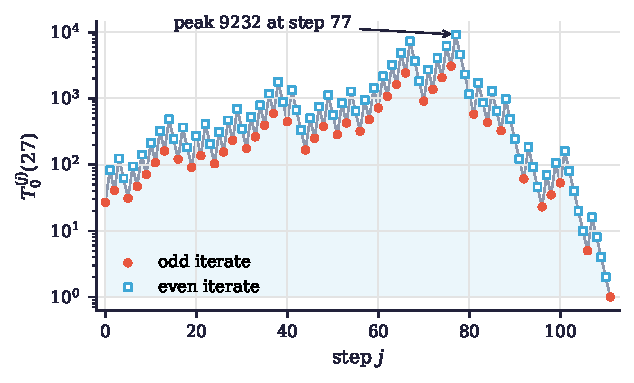
\includegraphics[width=\textwidth]{figures/ch1_orbit27.pdf}
\caption{The orbit of $27$ under the standard map $T_0$, on a logarithmic scale. Iterates are marked by parity: every odd iterate $x$ is followed by a rise to $3x+1$ and every even iterate by a halving, so the odd iterates are the points where the path turns upward. The orbit takes $111$ steps to reach $1$ and peaks at $9232$ after $77$ steps.}
\label{fig:ch1:orbit27}
\end{figure}

The counts in this example already contain most of the arithmetic we shall
need. Because each tripling is followed by at least one halving, the same orbit
takes $111-41=70$ steps under the accelerated map\index{accelerated map} $T$ and $41$ steps under the
Syracuse map\index{Syracuse map} $S$. Each tripling multiplies by slightly more than $3$ and each
halving divides by exactly $2$, so an orbit with $41$ triplings and $70$
halvings that starts at $27$ and ends at $1$ must have $27\cdot3^{41}$ a little
below $2^{70}$. Indeed $27\cdot3^{41}/2^{70}\approx0.834$, and the gap from
$1$ is made up by the additive ones. We make this exact in
\cref{chap:parity}, where we show that $2^k T^{(k)}(n)=3^m n+c_k(n)$ under
the accelerated map, with $m$ the number of odd steps among the first $k$ and
$c_k(n)$ an explicit integer, positive as soon as $m>0$, built from the
positions of the odd steps.

The orbit of $27$ is also a reminder that orbits merge. The orbit of $97$
reaches $94$ after $13$ steps; the orbit of $27$ reaches $94$ after $6$ steps;
from $94$ onward the two coincide. Hence $\sigma_\infty(97)=13+105=118$ and
the orbit of $97$ peaks at $9232$ as well.
The orbits that reach $1$ form a tree rooted at $1$, once the edge from $1$ to $4$ is removed; it is a component of the \emph{Collatz graph}, which joins each $n$ to $T_0(n)$, and the conjecture says that this tree contains every positive integer.

\paragraph{Records.} A starting value $n$ is a \emph{delay record} if
$\sigma_\infty(n)>\sigma_\infty(n')$ for every $n'<n$. The delay records up to
$10^5$ are
\[
\begin{aligned}
&1,\,2,\,3,\,6,\,7,\,9,\,18,\,25,\,27,\,54,\,73,\,97,\,129,\,171,\,231,\\
&313,\,327,\,649,\,703,\,871,\,1161,\,2223,\,2463,\,2919,\,3711,\\
&6171,\,10971,\,13255,\,17647,\,23529,\,26623,\\
&34239,\,35655,\,52527,\,77031.
\end{aligned}
\]
\cref{tab:ch1:records} lists a selection with their total stopping times\index{stopping time} and
peaks. The longest orbit below $10^4$ starts at $6171$ and takes $261$ steps;
below $10^5$ it starts at $77031$ and takes $350$ steps; below $10^6$ it starts
at $837799$ and takes $524$ steps. Peaks can be enormous relative to the
starting value: below $10^4$ the highest point reached by any orbit is
$27\,114\,424$, from $n=9663$, and below $10^5$ it is $1\,570\,824\,736$, from
$n=77671$.

\begin{table}[t]
\centering
\caption{Selected delay records for the standard map $T_0$: total stopping
time $\sigma_\infty(n)$ and the largest value in the orbit.}
\label{tab:ch1:records}
\begin{tabular}{@{}rrr@{}}
\toprule
$n$ & $\sigma_\infty(n)$ & $\max_k T_0^{(k)}(n)$ \\
\midrule
$7$ & $16$ & $52$ \\
$9$ & $19$ & $52$ \\
$27$ & $111$ & $9\,232$ \\
$97$ & $118$ & $9\,232$ \\
$871$ & $178$ & $190\,996$ \\
$6\,171$ & $261$ & $975\,400$ \\
$77\,031$ & $350$ & $21\,933\,016$ \\
$837\,799$ & $524$ & $2\,974\,984\,576$ \\
\bottomrule
\end{tabular}
\end{table}

\paragraph{How long do orbits take?} \cref{fig:ch1:totalstop} plots
$\sigma_\infty(n)$ for all $n\leq10^5$ against $\log n$. Two features stand
out. The points fill a band whose centre grows linearly in $\log n$, and the
band is wide, with a visible fine structure of streaks caused by merging
orbits. The linear growth is predicted by the simplest probabilistic model.
Under $T_0$ an odd value is always followed by an even one, and on average
about one step in three is odd. If we pretend that the parities are random
with $\Prob(\text{odd})=1/3$, each step changes $\log x$ by $\log3$ (ignoring
the $+1$) with probability $1/3$ and by $-\log2$ with probability $2/3$, so the
mean change per step is
\[
  \tfrac13\log3-\tfrac23\log2=\tfrac13\log\tfrac34\approx-0.0959.
\]
An orbit starting at $n$ should therefore need about
\[
  \frac{3\log n}{\log(4/3)}\approx10.43\log n
\]
steps, which is the line drawn in the figure.
The least squares line through the origin fitted to $\sigma_\infty(n)$ against $\log n$ over $2\leq n\leq10^4$ has slope $10.36$, and over the range $2\leq n\leq10^5$ of \cref{fig:ch1:totalstop} it has slope $10.23$.
For the accelerated map, whose heuristic slope is $2/\log(4/3)=1/|\ds|\approx6.952$ with $\ds=\log(\sqrt3/2)$, the fitted slopes over the same two ranges are $6.920$ and $6.837$.
The constant
$\ds$ will be a central character in \cref{chap:stochastic}.

\begin{figure}[t]
\centering
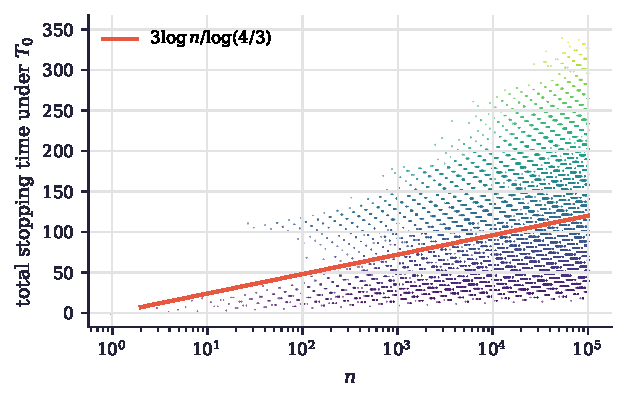
\includegraphics[width=\textwidth]{figures/ch1_totalstop.pdf}
\caption{Total stopping times $\sigma_\infty(n)$ under $T_0$ for all $n\leq10^5$, with $n$ on a logarithmic scale. The solid line is the prediction $3\log n/\log(4/3)$ of the random parity model. The streaks are families of starting values whose orbits merge after a few steps.}
\label{fig:ch1:totalstop}
\end{figure}

The agreement between heuristic and computation is good, and it is worth
being clear about what it does and does not mean.
It is consistent with the parities of the accelerated map along a typical orbit having the frequencies of fair coin flips, so that one step of $T_0$ in three is odd.
It does not
mean that any particular orbit must descend, and it gives no handle at all on
the question of whether some exceptional orbit could avoid $1$ forever. The
heuristic averages over starting values, while the conjecture is about every
starting value. That gap recurs in every chapter of this book.

\section{Computational verification}\label{sec:ch1:verification}

Because the conjecture is a universal statement about integers, it invites
computation, and the problem has been checked by computer for almost as long
as there have been computers. Each verification establishes that every $n$ up
to some bound $X$ reaches $1$. The techniques are clever: one need only check
that each $n$ eventually falls below itself, since smaller values have already
been handled; residue classes that provably fall below their starting value in
a few steps can be skipped wholesale, which is the idea behind the stopping
time analysis of \cref{chap:parity}; and the accelerated and Syracuse forms
let one take several steps at once using precomputed tables indexed by
residues modulo a power of $2$.

The bounds have grown by many orders of magnitude. In the 2000s Oliveira e Silva\index{Oliveira e Silva, T.}
verified the conjecture up to $5\cdot2^{60}\approx5.76\times10^{18}$, an effort
described in his chapter of the Lagarias\index{Lagarias, J. C.} volume~\cite{oliveira2010}. In 2021
Ba\v{r}ina\index{Barina, D.@Ba\v{r}ina, D.}~\cite{barina2021} reported verification up to $2^{68}\approx
2.95\times10^{20}$, using a carefully optimized algorithm on graphics
processors, and in 2025 he extended it to
$2^{71}\approx2.36\times10^{21}$~\cite{barina2025}. Most of the computations
in this book use the range $2^{68}$: whenever we say \emph{the verified range\index{verification range}} we
mean that every $n\leq2^{68}$ is known to reach $1$. We shall see that the
sharp form of the cycle bound below is the same at $2^{71}$.

Verification has two consequences beyond the obvious one. First, any orbit
that fails to reach $1$ must stay above $2^{68}$ forever, because if it ever
dropped to $2^{68}$ or below it would join a verified orbit. In particular a
nontrivial cycle would have least element above $2^{68}$. Second, and less
obviously, this lower bound on the least element can be converted into a lower
bound on the length of a cycle, by an argument going back to
Crandall\index{Crandall, R. E.}~\cite{crandall1978} and
Eliahou\index{Eliahou, S.}~\cite{eliahou1993} that uses the continued fraction\index{continued fraction} of $\lt$. In
\cref{chap:cycles} we carry out this argument in detail.
A first version, the block form of the bound, which uses only the convergents\index{convergent} of $\lt$, shows that with the verified range $2^{68}$ every nontrivial cycle contains at least $6\,586\,818\,670$ odd terms.
A sharper version, which uses a short mediant lemma\index{mediant lemma} together with the classical description of the best one sided approximations~\cite[Theorem~4.5(ii)]{hancl2019}, both proved in \cref{chap:cycles}, to show that the extremal cases always occur at intermediate fractions\index{semiconvergent} of the continued fraction lying above $\lt$,
gives unconditionally
\[
  r\;\geq\;72\,057\,431\,991
\]
for the number $r$ of odd terms in any nontrivial cycle. It coincides with the
bound $r>7.2\times10^{10}$ that Hercher\index{Hercher, C.}~\cite{hercher2023} credits to
Hercher and Puchert\index{Puchert, S.}~\cite{hercher2018,puchert2018}. Applied to Eliahou's
verification range $2^{40}$, the same method returns exactly his lower bound
$17\,087\,915$ on the length of a cycle of the accelerated map\index{accelerated map}. The
current record is larger still: Hercher~\cite[Corollary~29]{hercher2023}
showed, by a sharper accounting of the structure of a cycle, that verification
up to $1536\cdot2^{60}=3\cdot2^{69}$ gives $r\geq1.375\times10^{11}$, and
Ba\v{r}ina's verification to $2^{71}$~\cite{barina2025} has made this
unconditional. Cycles, if they exist, are very long and live very
high up.

Verification can never prove the conjecture, and it is not even clear what
evidential weight it carries. Orbits that misbehave, if they exist, might
start at numbers so large that no computation will ever reach them. The
heuristic of \cref{sec:ch1:orbits} predicts that the longest orbits below $N$
take time of order $\log N$, so nothing in the data suggests a change of
regime, but one should remember that the problem has a large supply of
quantities that grow like $\log N$ or $\log\log N$, and phenomena governed by
such quantities can hide far beyond the reach of any computer.

\section{Undecidability: Conway's theorem}\label{sec:ch1:conway}

Why should such a simple problem be hard? One answer is that the class of
problems it belongs to contains problems that are not merely hard but
impossible. In 1972 Conway\index{Conway, J. H.}~\cite{conway1972} considered \emph{generalized
Collatz maps}: fix a modulus $p\geq2$ and rational numbers $a_0,\ldots,a_{p-1}$
and $b_0,\ldots,b_{p-1}$, chosen so that
\[
  g(n)=a_i n+b_i \qquad\text{whenever } n\equiv i\pmod p
\]
maps integers to integers. The Collatz map is the case $p=2$, $a_0=1/2$,
$b_0=0$, $a_1=3$, $b_1=1$. Conway showed that this class is rich enough to
simulate any computation: given a Turing machine one can construct such a $g$
whose iterates encode the steps of the machine. It follows that there is no
algorithm which, given $g$ in this class and a starting value $n$, decides
whether the orbit of $n$ under $g$ eventually reaches $1$. Conway's
construction in fact needs only the maps with all $b_i=0$, which multiply by a
rational depending on the residue class.

Conway later packaged this observation as a programming language,
FRACTRAN\index{FRACTRAN}~\cite{conway1987}. A FRACTRAN program is a finite list of fractions
$q_1,\ldots,q_t$; the state is a positive integer $n$; one step replaces $n$ by
$q_i n$ for the first $i$ such that $q_i n$ is an integer, and the program halts
if there is none. Each such step is a generalized Collatz map with all $b_i=0$
and modulus the least common multiple of the denominators. Conway exhibited a
FRACTRAN program of fourteen fractions whose orbit starting at $2$ passes
through exactly the powers of $2$ with prime exponent, in increasing order,
and showed that FRACTRAN is a universal model of computation. Kurtz\index{Kurtz, S. A.} and
Simon\index{Simon, J.}~\cite{kurtz2007} sharpened the logical classification, showing that the
generalized problem of deciding whether every orbit of a given $g$ reaches $1$
is complete for the class $\Pi^0_2$ of the arithmetic hierarchy.

None of this says that the original problem is undecidable, and indeed a
single statement such as \cref{conj:ch1:collatz} is either true or false; the
undecidability concerns algorithms that work uniformly over the whole class.
What Conway's theorem does say is that any proof of the Collatz conjecture\index{Collatz conjecture}
must use something specific about the numbers $2$ and $3$. Soft arguments
that would apply equally to every map of the form $a_i n+b_i$ cannot work,
because for some maps in the class the corresponding statement is false, and for every sound, recursively axiomatized theory there are maps for which it is true but not provable in that theory.
This is the
theoretical counterpart of the observation about negative integers\index{negative cycles} above.
In this book the specific arithmetic of $2$ and $3$ enters in three places:
the Geometric law of $\vt(3n+1)$ in \cref{chap:parity}, through the comparison of its mean $2$ with $\lt$ (the same law holds for $\vt(5n+1)$, but $\log_25>2$), the identity
$\tfrac12\cdot\tfrac12+\tfrac12\cdot\tfrac32=1$ behind the martingale\index{martingale} of
\cref{chap:stochastic}, and the continued fraction\index{continued fraction} of $\lt$ in
\cref{chap:cycles}.

\section{What is known: density theorems}\label{sec:ch1:density}

Since proving the conjecture for every $n$ is out of reach, a natural weakening
is to prove it for almost every $n$, in some sense of density. Recall that a
set $A\subseteq\N$ has \emph{natural density} $\delta$ if
$\#\{n\leq x:n\in A\}/x\to\delta$ as $x\to\infty$, and \emph{logarithmic
density} $\delta$ if
\[
  \frac{1}{\log x}\sum_{n\leq x,\ n\in A}\frac1n\;\longrightarrow\;\delta .
\]
Natural density $1$ implies logarithmic density $1$, but not conversely, so
logarithmic density statements are weaker.

\paragraph{Terras and Everett.} The first theorem of this type concerns the
\emph{stopping time\index{stopping time}} $\sigma(n)$, the least $k\geq1$ with $T^{(k)}(n)<n$ under
the accelerated map\index{accelerated map}. Terras\index{Terras, R.}~\cite{terras1976,terras1979} and, independently,
Everett\index{Everett, C. J.}~\cite{everett1977} proved that the set of $n$ with $\sigma(n)<\infty$
has natural density $1$. Terras proved more: for each $k$ the set
$\{n:\sigma(n)\leq k\}$ has a natural density $F(k)$, and $F(k)\to1$. The key
idea, common to both, is that the first $k$ parities of the orbit of $n$ depend only on $n$
modulo $2^k$, and that every pattern of $k$ parities occurs for exactly one
residue class~\cite[Theorem~B]{lagarias1985}. We prove all of this in \cref{chap:parity}, where it is
\cref{thm:terras} and \cref{thm:density}. A stopping time result is weaker than
it looks: it says that almost every orbit eventually goes below its starting
value, which, applied repeatedly, does not show that almost every orbit reaches
$1$, because the exceptional set at each stage could catch the orbit.

\paragraph{Smaller and smaller.} Later work showed that almost all orbits go
much lower. Korec\index{Korec, I.}~\cite{korec1994} proved that for every
$\theta>\log3/\log4\approx0.7925$ the set of $n$ whose orbit contains a value
below $n^{\theta}$ has natural density $1$. The exponent $\log3/\log4$ has the
same source as the drift\index{drift} $\log(3/4)$ of the Syracuse map\index{Syracuse map} that we compute in
\cref{chap:parity}.

\paragraph{Krasikov and Lagarias.} A different kind of result counts the
integers that are known to reach $1$. Writing $\pi_1(x)$ for the number of
$n\leq x$ whose orbit contains $1$, Krasikov\index{Krasikov, I.} and Lagarias\index{Lagarias, J. C.}~\cite{krasikov2003}
proved, by a system of difference inequalities\index{difference inequality} derived from the structure of
the Collatz graph modulo powers of $3$, that $\pi_1(x)\geq x^{0.84}$ for all
sufficiently large $x$. This is far from density $1$, but it is a statement
about orbits that actually reach $1$, not merely orbits that descend.

\paragraph{Tao.} The strongest result to date is due to Tao. For the smallest
value attained by the orbit of $n$ under the standard map\index{standard map} we write
\[
  \mathrm{Col}_{\min}(n)=\min_{k\geq0}T_0^{(k)}(n).
\]

\begin{theorem}[{Tao~\cite[Theorem~1.3]{tao2022}}]\label{thm:ch1:tao}
Let $f:\N\to\R$ be any function with $f(n)\to\infty$ as $n\to\infty$. Then
\[
  \mathrm{Col}_{\min}(n)<f(n)
\]
for all $n$ in a set of logarithmic density $1$.
\end{theorem}

Taking $f(n)=\log\log\log\log n$, for example, the theorem says that almost
every orbit, in logarithmic density, eventually dips below
$\log\log\log\log n$. This is the sense of the title of Tao\index{Tao, T.}'s paper: almost all
orbits attain almost bounded values. It is a remarkable strengthening of the
Terras and Korec results, which give the weaker bounds
$\mathrm{Col}_{\min}(n)<n$ and
$\mathrm{Col}_{\min}(n)<n^{\theta}$. The proof works with the Syracuse map. Its
deep input is a fine scale mixing
estimate~\cite[Proposition~1.14]{tao2022}: the residues modulo powers of $3$ of the
Syracuse iterates of a suitably random starting value are governed by a certain
\emph{Syracuse random variable} that encodes the first few Syracuse steps, and
this variable is approximately equidistributed\index{equidistribution} at fine $3$ adic scales,
although far from uniform at coarse ones~\cite[Remark~1.15]{tao2022}. The key
estimate is a decay bound for its characteristic function. The fine scale
mixing is then fed into an iterative argument that pushes the orbit
down from scale $n$ to scale $n^{\alpha}$ for some $\alpha<1$, many times over.

Three limitations of \cref{thm:ch1:tao} illustrate the general difficulty. It concerns logarithmic density, not
natural density. It shows that orbits become small, not that they reach $1$;
to conclude that they reach $1$ one would need to know that every orbit below
some fixed bound reaches $1$, which is a finite computation, but the bound
$f(n)$ depends on $n$ and the exceptional set depends on $f$. Most importantly,
it is a statement about almost all starting values, and like every density
theorem it is silent about any individual orbit. The conjecture asserts
something about every integer, and no density statement, however strong,
reaches every integer.

\section{The two halves and the heuristic}\label{sec:ch1:heuristic}

We can now state the heuristic that organizes the subject, and the reason it is
not a proof.

Under the accelerated map\index{accelerated map}, an odd step multiplies by roughly $3/2$ and an even
step divides by $2$. If the parities along an orbit behaved like independent
fair coin flips, then $\log T^{(k)}(n)$ would be a random walk with increments
$\log(3/2)$ and $-\log2$, each with probability $\tfrac12$, and drift\index{drift}
\[
  \ds=\tfrac12\log\tfrac32-\tfrac12\log2=\log\frac{\sqrt3}{2}\approx-0.1438.
\]
A random walk with negative drift goes to $-\infty$, so almost every orbit
would descend, and since the orbit is bounded below by $1$ it would end in the
trivial cycle. This is the heuristic of Crandall\index{Crandall, R. E.}~\cite{crandall1978} and of
Lagarias\index{Lagarias, J. C.} and
Weiss\index{Weiss, A.}~\cite{lagarias1992}, and \cref{chap:stochastic} develops it
carefully. Its predictions agree closely with computation where they can be tested. It predicts the slope of \cref{fig:ch1:totalstop}, $3/\log(4/3)$ steps of $T_0$ per unit of $\log n$, which is $1/|\ds|$ steps of $T$, to within about two percent; it predicts the Geometric distribution of $\vt(3n+1)$, which in \cref{chap:parity} we prove exactly for residue classes; and it predicts the autocorrelations $(-\tfrac12)^h$ of the parity sequence of $T_0$ (\cref{sec:ch3:autocorr}), which orbits of large integers reproduce over the range where the model is exact, while full orbits of small integers reproduce them only at lags $1$ and $2$, where the agreement is forced or reflects a single stride.

It is not a proof because the parity sequence of an orbit is not random. It is
a deterministic function of the starting value. The model is exactly right
for a uniformly random starting residue modulo $2^k$ and the first $k$ steps,
which is the content of the Terras bijection, and it is no longer justified after that
because the orbit of a fixed integer is a single sample path, not an ensemble.
No known theorem converts the statistics of residue classes into statements
about a single path.
Every serious attack on the divergence half is, in one form or another, an attempt to close that gap.

The two halves of the conjecture interact with the heuristic differently. The
divergence half asks whether $\log T^{(k)}(n)$ can drift upward forever.
This is a law of large numbers question: in Syracuse form, an orbit can be unbounded only if the running average of the halving exponents $\vt(3y+1)$ along it has lower limit at most $\lt\approx1.585$ (\cref{prop:cesaro,cor:ch9:freq}), so the divergence half is equivalent to the Ces\`aro liminf conjecture (\cref{conj:cesaro}) that this lower limit always exceeds $\lt$; under the Geometric law the average is $2$.
The cycle half asks whether an orbit can close up. That is not an
averaging question at all. A cycle imposes an exact multiplicative identity,
which after taking logarithms says that $s\log2-r\log3$ is positive and very
small for the number $r$ of odd steps and $s$ of halvings in the cycle. The
first tools are Diophantine\index{Diophantine approximation}, through the rational approximations of $\lt$,
but we shall see that they can never suffice on their own: arithmetic
information about the parity word is also needed.

\section{Machine checked mathematics}\label{sec:ch1:lean}

Machine checking is changing how results about problems like this one are verified, and we use it in this book. Proof assistants such as Lean\index{Lean} allow a theorem and its
proof to be written in a formal language and checked mechanically by a small
trusted kernel. In 2026 Google DeepMind described \emph{AlphaProof
Nexus}~\cite{tsoukalas2026}, a system that couples a large language model to
the Lean compiler: the model edits a Lean file containing an unproved
statement, receives the compiler's messages, and continues until a complete
proof is found or a budget is exhausted. Run over $353$ formalized problems
from the collection of problems posed by Erd\H{o}s, it produced complete
formal solutions to nine, among them Erd\H{o}s problem $125$ on the
lower density of the sumset of the integers whose base $3$ digits lie in
$\{0,1\}$ and those whose base $4$ digits lie in $\{0,1\}$; the answer is that
the lower density is zero.
That proof turns on good rational approximations to $\log4/\log3=2/\lt$, the same kind of Diophantine\index{Diophantine approximation} object that appears in the cycle problem, where it plays the opposite role.
For Erd\H{o}s $125$ the existence of good approximations drives the density down.
For Collatz cycles good approximations are what a cycle needs, they exist for infinitely many cycle lengths at every verification range (\cref{prop:ch8:insufficient}), and excluding cycles needs arithmetic information about the parity word that no bound on the quality of approximation supplies.

We claim nothing more for this than it delivers. AlphaProof Nexus\index{AlphaProof Nexus} does not
address the Collatz conjecture\index{Collatz conjecture}, and we know of no automated result that bears
on it directly. What machine checking does offer is a reliable record of exactly what has
and has not been proved. In this spirit we have written Lean statements of the
Collatz conjecture, of its descent form and of the cycle problem, together
with machine checked proofs of some elementary ingredients, among them the
affine identity for iterates proved in \cref{chap:parity} and the inequality
$3^r<2^s$ satisfied by any cycle of positive integers; these are described in \cref{sec:ch8:lean}, following our note~\cite{polsonsokolov2026nexus}.

\section{What this book does}\label{sec:ch1:plan}

We should be direct about the status of what follows. This book does not prove
the Collatz conjecture\index{Collatz conjecture}. It does four other things.

It \emph{organizes} the known heuristics into a single framework in which the
dynamics are read as an optimization method: a potential function $\log x$
that the iteration tries to decrease, a move that increases it (the odd step),
and moves that decrease it (the halvings). In that language the two halves of
the conjecture become the two ways an optimizer can fail: the iterates run
away, or they enter a limit cycle.

It \emph{makes the constants explicit}: the drift\index{drift} $\ds=\log(\sqrt3/2)$, the
step variance, the Syracuse drift $\log(3/4)$, the stride ratio
$\kappa=\log(5/3)/|\log(3/4)|\approx1.776$ of the largest ascent of a stride to its mean descent, the parity autocorrelation\index{autocorrelation} $(-\tfrac12)^h$, and the
exact mixing\index{mixing} time of the model chain on the units modulo $3^a$, in which the
halving exponents are independent Geometric$(\tfrac12)$ draws.
These matter because any heuristic for the conjecture must be consistent with them; a heuristic predicting a different drift can be discarded at once.

It \emph{proves structural results}, most of them short and several of them
classical. Some are positive, such as the Terras\index{Terras, R.}
bijection, the exact Geometric law, the martingale\index{martingale} duality and the closed
form of the parity autocorrelations in the model. Some are negative: no
monotone Lyapunov function\index{Lyapunov function} certifies descent over any fixed number of
Syracuse strides, the
natural majorization\index{majorization} of $\log x$ drifts the wrong way in the model, and the
martingale of the model fails to be uniformly integrable\index{uniform integrability}. Each negative
result shows where a natural line of attack stops.

And it \emph{sharpens} the questions. For the cycle half it proves that
Diophantine\index{Diophantine approximation} approximation of $\lt$, however strong, combined with any finite
verification can exclude only finitely many cycle lengths, a point that
Halbeisen\index{Halbeisen, L.} and Hungerb\"uhler\index{Hungerbuhler, N.@Hungerb\"uhler, N.}~\cite[\S5]{halbeisen1997} made in another
form; it then shows,
through a window lemma\index{window lemma}, that an arithmetic improvement of the basic cycle
inequality by a factor slightly larger than $r/3$, combined with a finite verification, would exclude all cycles.
The divergence half is restated exactly as a conjecture about the lower limit of the Ces\`aro averages of halving exponents (\cref{conj:cesaro}), which we can state but cannot prove.

\paragraph{Plan of the book.} The book has three parts.

Part I, \emph{The Problem}, lays the foundations. \cref{chap:parity} sets out
the three maps, parity vectors\index{parity vector}, the Terras bijection, the exact Geometric law
of $\vt(3n+1)$, the $2$ adic extension and its conjugacy to the shift, and the
density theorem\index{density theorem} of Terras and Everett\index{Everett, C. J.} with a complete proof.
\cref{chap:stochastic} develops the stochastic model and the martingale
duality: under the Bernoulli model\index{Bernoulli model} the iterates form a multiplicative
martingale, because $\tfrac12\cdot\tfrac12+\tfrac12\cdot\tfrac32=1$ exactly,
while their logarithms form a strict supermartingale\index{supermartingale} with drift $\ds$. The gap
is Jensen's inequality\index{Jensen inequality}. We also compute the parity autocorrelations in closed
form and show that the martingale is not uniformly integrable.

Part II, \emph{The Optimization Reading}, takes the analogy with optimization
seriously and pushes it until it breaks. \cref{chap:lyapunov} treats
$\log x$ as a Lyapunov function, proves the exact stride descent inequality,
and proves that no monotone Lyapunov function certifies descent over any
fixed number of strides; it also shows that
under the stochastic model the linear majorizer of the MM framework\index{MM algorithm}~\cite{lange2000,hunter2004} has positive mean increment while the potential has negative drift.
\cref{chap:momentum}
makes the analogy with Nesterov\index{Nesterov acceleration} momentum\index{momentum}~\cite{nesterov1983,su2016} precise
at the level of strides and is explicit about its limits: the stride ratio is
a ratio of increments, not a condition number\index{condition number}.
\cref{chap:mmcollatz} presses the majorization idea on the Collatz map itself: the multiplicative majorizer reproduces the cycle inequality, and three impossibility results show that no correction of $\log x$ by a function of $x$ modulo a fixed power of $2$ certifies descent, that any correction that certifies it must be unbounded, and that a penalty proportional to the number of trailing ones in the binary expansion of $x$ fails at a positive fraction of odd integers for every weight.
\Cref{chap:smm,chap:noise} then run the analogy in the other direction. The Collatz
arithmetic suggests an optimizer, \emph{Switching MM\index{Switching MM}}, which alternates a
plain gradient step with a momentum step according to the parity of the
iteration counter, with momentum constant
\[
  \beta=\frac{\log(3/2)}{\log2}=\lt-1\approx0.585,
\]
the ratio of the ascent of an odd step to the descent of an even step. We show
that on quadratics two steps of Switching MM are exactly two gradient steps
with step sizes $\alpha$ and $(1+\beta)\alpha$, so that the method is a cyclic
step size schedule, and we compute its stationary variance under gradient
noise exactly. Its noise amplification relative to gradient descent at the same step is bounded
by $5/3$ for every $\beta<1$, whereas in the slow modes every step momentum amplifies noise by
$1/(1-\beta)$. Nothing in these two chapters bears on the conjecture; they are
an instance of number theory suggesting a design.
\Cref{chap:difference} closes Part II by treating both the Collatz recursion and the momentum methods as nonlinear difference equations: it derives certified growth exponents for the inverse tree\index{inverse tree} from difference inequalities\index{difference inequality} in the style of Krasikov\index{Krasikov, I.} and Lagarias\index{Lagarias, J. C.}, computes the joint spectral radius\index{joint spectral radius} that governs the stability of Switching MM under arbitrary switching, which is below one at every parameter value computed, and proves a linear rate for Switching MM on smooth strongly convex functions that is the exact worst case for the distance to the minimizer.

Part III, \emph{Cycles and Divergence}, returns to the conjecture.
\cref{chap:cycles} treats the cycle half through the continued fraction\index{continued fraction} of
$\lt$, derives the cycle length bounds quoted in \cref{sec:ch1:verification}
from the verified range\index{verification range}, and places them in the literature from
Crandall\index{Crandall, R. E.}~\cite{crandall1978} and Steiner\index{Steiner, R. P.}~\cite{steiner1977} through Eliahou\index{Eliahou, S.}, Simons\index{Simons, J.} and de
Weger\index{de Weger, B.}~\cite{simons2005}, and Hercher\index{Hercher, C.} and Puchert\index{Puchert, S.}. The key ingredient is a mediant lemma\index{mediant lemma}
which, with the one sided theorem of that chapter, gives a short proof of the classical fact that the first cycle length not excluded
by a given verification range is always a rung of the semiconvergent\index{convergent}\index{semiconvergent} ladder
that approximates $\lt$ from above; it makes the computation rigorous and yields the
unconditional bound $r\geq72\,057\,431\,991$. The method is that of Crandall
and Eliahou, the bound coincides with that of Hercher and Puchert, and it
remains below Hercher's current record. An exact integer certificate\index{certificate} for the bound is given. The chapter then
proves that Diophantine information about $\lt$ alone cannot finish the cycle half, and locates
the least element of any cycle in a window whose width, a factor of about
$r/3$, measures exactly what is missing. \cref{chap:divergence} treats the divergence half
through the Ces\`aro averages of halving exponents, proves that the natural
Ces\`aro criterion holds automatically at the stride at which an orbit terminates (so that verifying it numerically on terminating orbits carries no information), formulates the
conjecture that would close this half, and shows that the model chain on
the units modulo $3^a$, in which the halving exponents are independent
Geometric$(\tfrac12)$ draws, is exactly stationary after $a$ strides, a
restatement in Markov chain form of an identity of
Tao\index{Tao, T.}~\cite[eq.~(1.21)]{tao2022}. \cref{chap:path} assembles what a proof would have
to contain, \cref{chap:computation} sets out what computation can and cannot contribute, with the guidance the optimization reading gives it, \cref{chap:samplers} tests level set samplers against the map and finds the horizon at which they fail, and \cref{chap:open} collects open problems and computational
projects.
A gallery of computed pictures, \emph{A Gallery of Orbits}, follows Part III, and the appendices tabulate the constants and describe the code.

\paragraph{How to read this book.} A reader interested mainly in the optimizer can read \cref{chap:momentum,chap:smm,chap:noise} and then \cref{chap:difference}, which uses their results, turning back to Part I and \cref{chap:lyapunov} for the stride arithmetic from which the momentum constant is derived. A reader interested mainly in the number theory can go from \cref{chap:parity} directly to \cref{chap:cycles}, and needs \cref{chap:stochastic} before \cref{chap:divergence}; before \cref{chap:path,chap:computation} this reader also needs the impossibility results of \cref{chap:lyapunov,chap:mmcollatz} and the first two sections of \cref{chap:difference}, on which \cref{chap:computation} builds; its comparisons with Switching MM also cite \cref{sec:ch5b:stability}. Every chapter ends with notes on the literature, and every chapter except \cref{chap:open} with exercises. The numbers we compute can be reproduced with the code described in \cref{app:code}.

\section*{Notes}

The history in \cref{sec:ch1:history} follows Lagarias\index{Lagarias, J. C.}~\cite{lagarias1985} and
the introductory chapters of~\cite{lagarias2010}, which also discuss the many
names of the problem and their origins in more detail than we have. The
annotated bibliographies~\cite{lagarias2003bib,lagarias2006bib} are the
quickest way into the specialized literature.

The stochastic models that underlie the heuristic of
\cref{sec:ch1:heuristic} are developed by Lagarias and Weiss~\cite{lagarias1992} and surveyed by Kontorovich\index{Kontorovich, A. V.} and Lagarias~\cite{kontorovich2009}; the survey also treats
the $5x+1$ problem, where the analogous model predicts divergence for almost
all orbits, a useful sanity check on any argument for the $3x+1$ case.

The original paper of Conway\index{Conway, J. H.}~\cite{conway1972} is short and readable, and
the FRACTRAN\index{FRACTRAN} paper~\cite{conway1987} contains the prime generating program and the
universality argument. The undecidability results show that the arithmetic of
$2$ and $3$ must enter any proof, and the reader can locate exactly where it enters each argument in this book.

Tao\index{Tao, T.}'s paper~\cite{tao2022} is long but carefully written; its
introduction gives an excellent account of why density methods stop short of
the full conjecture. The equidistribution\index{equidistribution} it proves is $3$ adic and holds
only at fine scales~\cite[Proposition~1.14 and Remark~1.15]{tao2022}; the
equidistribution in \cref{chap:parity} is $2$ adic and much easier. Both are
statements about ensembles of starting values.

\section*{Exercises}

\begin{exercise}\label{ex:ch1:negative}
Find all cycles of $T_0$ on the integers $n$ with $|n|\leq1000$. For each
cycle record the number $r$ of odd terms and the number $s$ of even terms, and
check that $2^s>3^r$ for positive cycles and $2^s<3^r$ for negative ones.
Explain this sign rule by multiplying the relations $T_0(x)/x$ around the
cycle.
\end{exercise}

\begin{exercise}\label{ex:ch1:merge}
Show that if $n\equiv4\pmod6$ then $n$ has two preimages under $T_0$, namely
$2n$ and $(n-1)/3$, and otherwise only one. Deduce that the Collatz graph
branches only at vertices congruent to $4$ modulo $6$, and use this to explain
why the orbits of $27$ and $97$ in \cref{sec:ch1:orbits} merge.
\end{exercise}

\begin{exercise}\label{ex:ch1:heuristic}
Under the random parity model for $T_0$ in which an odd step is followed by an
even step and an even step is followed by an odd or even step with equal
probability, show that the long run fraction of odd steps is $1/3$. Deduce the
heuristic slope $3/\log(4/3)$ for $\sigma_\infty(n)$ against $\log n$, and
check numerically that the fraction of odd steps along the orbit of $27$ is
$41/111\approx0.369$.
\end{exercise}

\begin{exercise}\label{ex:ch1:fractran}
Consider the generalized Collatz map $g(n)=n/2$ for $n$ even and $g(n)=5n+1$
for $n$ odd.
Follow the orbits of $n\leq100$ until they repeat or exceed $10^{15}$, find the two cycles not containing $1$, and count the orbits that are still growing when you stop.
Repeat the heuristic computation of \cref{sec:ch1:heuristic}
for this map and show that the predicted drift\index{drift} of $\log x$ is positive.
\end{exercise}

\begin{exercise}\label{ex:ch1:verify}
Write a program that verifies \cref{conj:ch1:collatz} for all $n\leq10^7$ by
checking only that each $n\geq2$ eventually falls below $n$. Show that it
suffices to test odd $n\equiv3\pmod4$, and estimate the speedup obtained by
also skipping the residue classes modulo $2^k$ that fall below their starting
value within $k$ accelerated steps (after reading \cref{chap:parity}; see \cref{tab:ch2:residues}).
\end{exercise}

\chapter{Parity Vectors and the Syracuse Map}\label{chap:parity}

The rule ``halve if even, triple and add one if odd'' has two ingredients, a
multiplicative one and a parity test, and everything interesting about the
problem comes from the way they interact. This chapter isolates the parity
test. We record the sequence of parities along an orbit as a binary word, the
\emph{parity vector\index{parity vector}}, and show that over a block of $k$ steps the parity
vector and the residue of the starting value modulo $2^k$ determine each other
completely. This theorem of Terras\index{Terras, R.} and Everett\index{Everett, C. J.} is the single most useful fact about the
problem. It explains why the iteration looks random: a uniformly random
residue modulo $2^k$ produces a parity vector of $k$ independent fair coin
flips, exactly and not approximately. It gives the exact Geometric law of the
halving exponent $\vt(3n+1)$, the exact drift\index{drift} $\log(3/4)$ of the Syracuse
map, and, after passing to the $2$ adic integers, a conjugacy of the Collatz
map with the binary shift. And it yields the first genuine theorem about the
conjecture, that almost every positive integer eventually falls below itself.

All of these results are statements about ensembles of starting values. None
of them says anything about a particular orbit, and the reader should keep in
mind throughout the chapter where exactly that limitation enters.

\section{Three maps}\label{sec:ch2:maps}

\Cref{chap:intro} introduced three versions of the iteration. We now fix
them formally.

\begin{definition}[The three Collatz maps]\label{def:maps}
\leavevmode
\begin{enumerate}[label=(\roman*),leftmargin=2em]
\item The \emph{standard map} $T_0:\Z\to\Z$ is $T_0(n)=n/2$ for even $n$ and
  $T_0(n)=3n+1$ for odd $n$.
\item The \emph{accelerated map} $T:\Z\to\Z$ is $T(n)=n/2$ for even $n$ and
  $T(n)=(3n+1)/2$ for odd $n$.
\item The \emph{Syracuse map} $S$ is defined on odd integers by
  $S(n)=(3n+1)/2^{\vt(3n+1)}$, where $\vt(m)$ denotes the exponent of the
  largest power of $2$ dividing $m\neq0$. It maps odd integers to odd
  integers.
\end{enumerate}
We write $T_0^{(k)}$, $T^{(k)}$, $S^{(k)}$ for the $k$th iterates, with the
zeroth iterate the identity.
\end{definition}

The maps $T_0$ and $T$ are defined on all of $\Z$, the map $S$ on all odd
integers (since $3n+1\neq0$ for integer $n$), and all three send positive
integers to positive integers. The relations between them are
immediate from the definitions. For every integer $n$,
\begin{equation}\label{eq:ch2:TT0}
  T(n)=T_0^{(1+b)}(n),\qquad b=n\bmod2,
\end{equation}
because for odd $n$ the value $3n+1$ is even and $T$ simply performs the
forced halving at once. For odd $n$, with $k=\vt(3n+1)$,
\begin{equation}\label{eq:ch2:ST}
  S(n)=T^{(k)}(n)=T_0^{(k+1)}(n),
\end{equation}
since $T(n)=(3n+1)/2$ and the next $k-1$ values $(3n+1)/2^i$, $1\leq i<k$, are
even. Thus the orbit of $n$ under $T$ is obtained from its orbit under $T_0$
by deleting the even value that follows each odd value, and the orbit of an
odd $n$ under $S$ is the subsequence of odd values in either.

\begin{proposition}[Equivalence of the three maps]\label{prop:ch2:equiv}
Let $n\geq1$. The orbit of $n$ under $T_0$ contains $1$ if and only if its
orbit under $T$ contains $1$. If $n$ is odd, this happens if and only if its
orbit under $S$ contains $1$. If $n=2^a n'$ with $n'$ odd, the orbit of $n$
contains $1$ if and only if the orbit of $n'$ does.
\end{proposition}

\begin{proof}
The values deleted in passing from the $T_0$ orbit to the $T$ orbit are of the
form $3y+1$ with $y\geq1$ odd, hence at least $4$; so $1$ is never deleted, and
the two orbits contain $1$ together. For odd $n$, the $S$ orbit is the set of
odd values in the $T$ orbit, and $1$ is odd. Finally $T^{(a)}(2^a n')=n'$.
\end{proof}

Each map has its uses. The standard map\index{standard map} is the one in the statement of the
conjecture, and it has one structural property the others lack.

\begin{lemma}[No consecutive odd steps]\label{prop:nocons}
If $n$ is odd then $T_0(n)$ is even. Consequently the parity sequence
$b_j=T_0^{(j)}(n)\bmod2$ of any orbit of $T_0$ never contains two consecutive
ones.
\end{lemma}

\begin{proof}
If $n$ is odd then $3n$ is odd, so $3n+1$ is even.
\end{proof}

\Cref{prop:nocons} is trivial, but it is easy to transfer it by mistake to the
accelerated map\index{accelerated map}.

\begin{remark}[A pitfall: odd runs under the accelerated map]\label{rem:ch2:pitfall}
Under $T$ consecutive odd steps do occur. For odd $n$, $T(n)=(3n+1)/2$ is odd
exactly when $3n+1\equiv2\pmod4$, that is, when $n\equiv3\pmod4$. Thus
$T(3)=5$, $T(7)=11$, $T(11)=17$, and $T^{(2)}(7)=17>7$, an ascent over two
steps. A tempting but false argument runs: ``an odd step multiplies by about
$3/2$ and is followed by an even step dividing by $2$, so any two consecutive
steps of $T$ that begin with an odd one multiply by at most about $3/4$.'' The
first clause is true and the second is false, because under $T$ the halving
that follows the tripling has already been absorbed into the odd step. In fact
runs of odd steps under $T$ can be arbitrarily long: for $j\geq1$ and any odd
$a$, induction on $i$ gives
\[
  T^{(i)}(2^j a-1)=3^i2^{j-i}a-1,\qquad 0\leq i\leq j,
\]
so the orbit of $2^ja-1$ begins with $j$ consecutive odd steps and climbs to
$3^ja-1$. Any descent inequality over a fixed number of steps of $T$ must
accommodate these runs.
We return to this point in \cref{chap:lyapunov}: a Syracuse stride from an odd $x\geq3$, defined below, descends exactly when it contains at least two halvings (\cref{thm:stride}), and no fixed number of strides gives descent for every starting value (\cref{cor:ch4:multistride}).
\end{remark}

The Syracuse map\index{Syracuse map} compresses each passage from one odd value to the next, which we call a \emph{stride}, into a single step.
For odd $x$ write $k=\vt(3x+1)\geq1$. Then
\begin{equation}\label{eq:ch2:stride}
  \log S(x)-\log x=\log\Bigl(3+\frac1x\Bigr)-k\log2 .
\end{equation}
Since $2<3+1/x\leq4$ for $x\geq1$, the increment is positive when $k=1$ and
negative when $k\geq2$ (for $x=1$, $k=2$ and the increment is $0$). The whole
question of descent is therefore a question about how often the halving
exponent $k$ equals $1$, and about the sizes of the larger values.

\begin{example}[The orbit of $27$ under the three maps]\label{ex:ch2:27}
The orbit of $27$ reaches $1$ after $111$ steps of $T_0$, $70$ steps of $T$,
and $41$ steps of $S$. The $41$ halving exponents along the Syracuse orbit are
\[
\begin{gathered}
  1,2,1,1,1,1,2,2,1,2,1,1,2,1,1,1,2,3,1,1,2,\\
  1,2,1,1,1,1,1,3,1,1,1,4,2,2,4,3,1,1,5,4,
\end{gathered}
\]
with sum $70$ and mean $70/41\approx1.707$.
The mean is below $2$, the value predicted by the Geometric law of \cref{sec:ch2:geom}; the climb itself happens in the first $32$ strides, whose exponents have mean $44/32=1.375<\lt$ and which take the orbit to its largest odd value $3077$.
The overall mean is above $\lt\approx1.585$, which is forced, as we shall see in \cref{chap:divergence}, for any orbit that reaches $1$.
\end{example}

\section{Parity vectors and the Terras bijection}\label{sec:ch2:terras}

From now on, unless stated otherwise, we work with the accelerated map\index{accelerated map} $T$ on
$\Z$.

\begin{definition}[Parity vector]\label{def:ch2:parity}
For $n\in\Z$ and $k\geq1$, the \emph{parity vector\index{parity vector}} of length $k$ of $n$ is
\[
  v_k(n)=\bigl(n\bmod2,\ T(n)\bmod2,\ \ldots,\ T^{(k-1)}(n)\bmod2\bigr)\in\{0,1\}^k .
\]
We write $m_k(n)$ for the number of ones in $v_k(n)$, the number of odd steps
among the first $k$, and $m_0(n)=0$.
\end{definition}

For example $v_3(3)=(1,1,0)$, since $3\mapsto5\mapsto8$, and $v_4(5)=(1,0,0,0)$,
since $5\mapsto8\mapsto4\mapsto2$. The basic computation is the following
lemma, which says how the orbit of $x$ responds when $x$ is perturbed by a
multiple of a power of $2$.

\begin{lemma}[Perturbation by a power of two]\label{lem:ch2:perturb}
Let $x,a\in\Z$ and $j\geq0$. For $0\leq i\leq j$,
\[
  T^{(i)}(x+2^ja)=T^{(i)}(x)+3^{m_i(x)}\,2^{\,j-i}\,a .
\]
In particular, for $i<j$ the values $T^{(i)}(x+2^ja)$ and $T^{(i)}(x)$ have the
same parity, so $v_j(x+2^ja)=v_j(x)$.
\end{lemma}

\begin{proof}
Induction on $i$. For $i=0$ there is nothing to prove. Suppose the identity
holds for some $i<j$, and put $y=T^{(i)}(x)$ and $y'=T^{(i)}(x+2^ja)=
y+3^{m_i(x)}2^{j-i}a$. Since $j-i\geq1$, $y'\equiv y\pmod2$. If $y$ is even
then $T(y')=y/2+3^{m_i(x)}2^{j-i-1}a$ and $m_{i+1}(x)=m_i(x)$. If $y$ is odd
then
\[
  T(y')=\frac{3y+1}{2}+3^{m_i(x)+1}2^{j-i-1}a ,
\]
and $m_{i+1}(x)=m_i(x)+1$. In both cases the identity holds at $i+1$.
\end{proof}

\begin{theorem}[Terras~\cite{terras1976}, Everett~\cite{everett1977}]\label{thm:terras}
For every $k\geq1$, the parity vector $v_k(n)$ depends only on $n\bmod2^k$,
and the induced map
\[
  \Phi_k:\Z/2^k\Z\to\{0,1\}^k,\qquad n\bmod2^k\mapsto v_k(n),
\]
is a bijection.
\end{theorem}

\begin{proof}
That $v_k(n)$ depends only on $n\bmod2^k$ is the case $j=k$ of
\cref{lem:ch2:perturb}. For injectivity, suppose $0\leq x<x'<2^k$ and
$v_k(x)=v_k(x')$. Let $j=\vt(x'-x)$, so $0\leq j<k$ and $x'=x+2^ja$ with $a$
odd. By \cref{lem:ch2:perturb} with $i=j$,
\[
  T^{(j)}(x')-T^{(j)}(x)=3^{m_j(x)}a ,
\]
which is odd. Hence $T^{(j)}(x)$ and $T^{(j)}(x')$ have different parities,
and since $j\leq k-1$ the vectors $v_k(x)$ and $v_k(x')$ differ in position
$j$, a contradiction. An injective map between two sets with $2^k$ elements is
a bijection.
\end{proof}

The proof shows a little more, which we record because it is the form used in
\cref{sec:ch2:adic}: if $\vt(x'-x)=j$ then the parity vectors of $x$ and $x'$
agree in positions $0,\ldots,j-1$ and differ in position $j$.

\begin{example}[Small moduli]\label{ex:ch2:small}
For $k=3$ the bijection $\Phi_3$ is
\[
\begin{array}{c|cccccccc}
n\bmod8 & 0&1&2&3&4&5&6&7\\ \hline
v_3(n) & 000&101&010&110&001&100&011&111
\end{array}
\]
Every word of length $3$ appears exactly once. Note that $7$ has parity vector
$111$, three odd steps in a row, in line with \cref{rem:ch2:pitfall}.
\end{example}

\begin{corollary}[Exact randomness of the first $k$ parities]\label{cor:ch2:iid}
Let $n$ be uniformly distributed on $\{1,2,\ldots,2^kN\}$ for some $N\geq1$, or
on $\Z/2^k\Z$. Then the entries of $v_k(n)$ are independent Bernoulli random
variables with parameter $\tfrac12$. Consequently $m_k(n)$ has the binomial
law with parameters $k$ and $\tfrac12$.
\end{corollary}

\begin{proof}
In both cases $n\bmod2^k$ is uniform on $\Z/2^k\Z$, so by \cref{thm:terras}
$v_k(n)$ is uniform on $\{0,1\}^k$, which is the law of $k$ independent fair
bits.
\end{proof}

\Cref{cor:ch2:iid} is the precise sense in which the Collatz iteration is
random. It is exact, but it has a horizon: the first $k$ parities of $n$ are
random when $n$ is random modulo $2^k$, and no statement is made about step
$k+1$ and beyond unless $n$ is random modulo a higher power of $2$.
For $n$ random modulo $2^k$, each step uses up one bit of the residue, and after $k$ steps the randomness is exhausted.

\section{The affine form of an iterate}\label{sec:ch2:affine}

The second basic fact is that $k$ steps of $T$ act on $n$ as an affine map
whose coefficients depend only on the parity vector\index{parity vector}.

\begin{proposition}[Affine form]\label{prop:ch2:affine}
For $n\in\Z$ and $k\geq0$,
\begin{equation}\label{eq:ch2:affine}
  2^k\,T^{(k)}(n)=3^{m_k(n)}\,n+c_k(n),
\end{equation}
where $c_0(n)=0$ and
\begin{equation}\label{eq:ch2:crec}
  c_{k+1}(n)=\begin{cases}3\,c_k(n)+2^k, & T^{(k)}(n)\text{ odd},\\
  c_k(n), & T^{(k)}(n)\text{ even}.\end{cases}
\end{equation}
Explicitly, if the odd steps occur at positions $0\leq i_1<i_2<\cdots<i_m\leq
k-1$ of the parity vector, with $m=m_k(n)$, then
\begin{equation}\label{eq:ch2:cexplicit}
  c_k(n)=\sum_{j=1}^{m}3^{\,m-j}\,2^{\,i_j}.
\end{equation}
In particular $c_k(n)$ depends only on $v_k(n)$, it is a nonnegative integer,
and it is positive as soon as $m_k(n)>0$.
\end{proposition}

\begin{proof}
Induction on $k$; the case $k=0$ is trivial. Write $x=T^{(k)}(n)$ and
$m=m_k(n)$, and assume $2^kx=3^mn+c_k(n)$. If $x$ is even then
$2^{k+1}T(x)=2^kx$, so the identity holds at $k+1$ with $m_{k+1}=m$ and
$c_{k+1}=c_k$. If $x$ is odd then
\[
  2^{k+1}T(x)=2^k(3x+1)=3\cdot2^kx+2^k=3^{m+1}n+3c_k(n)+2^k,
\]
and $m_{k+1}=m+1$. Unwinding the recursion, the odd step at position $i_j$
contributes $2^{i_j}$, which is then multiplied by $3$ once for each of the
$m-j$ later odd steps; this is \eqref{eq:ch2:cexplicit}.
\end{proof}

The identity \eqref{eq:ch2:affine}, with the positivity of $c_k$, is simple
enough to be checked by machine, and we have done so: it is one of the
statements proved in the Lean\index{Lean} proof assistant, by exactly the induction above,
in the formalization described in \cref{chap:cycles}. There is a second,
multiplicative way to see the same quantity. Multiplying the ratios
$T(y)/y$ along the orbit, each even value contributes $1/2$ and each odd value
$y$ contributes $(3+1/y)/2$, so for $n\geq1$
\begin{equation}\label{eq:ch2:product}
  \frac{2^kT^{(k)}(n)}{3^{m}n}=\prod_{\substack{0\leq i<k\\ T^{(i)}(n)\text{ odd}}}
  \Bigl(1+\frac{1}{3T^{(i)}(n)}\Bigr),
\end{equation}
and hence $c_k(n)=3^mn\bigl(\prod(1+1/(3T^{(i)}(n)))-1\bigr)$, the product
running over the same odd values.
The additive ones of the iteration are thus a small multiplicative correction
when the odd values are large, and \eqref{eq:ch2:product} is the form we use
in \cref{chap:cycles}.

\begin{example}\label{ex:ch2:c27}
The orbit of $27$ reaches $1$ after $70$ steps of $T$, with $m_{70}(27)=41$.
Then \eqref{eq:ch2:affine} reads $2^{70}=3^{41}\cdot27+c_{70}(27)$, and indeed
the sum \eqref{eq:ch2:cexplicit} evaluates to
$c_{70}(27)=195\,820\,718\,533\,800\,070\,543=2^{70}-27\cdot3^{41}$, about
$0.166\cdot2^{70}$.
\end{example}

Two consequences of \cref{prop:ch2:affine} will be used repeatedly.

\begin{corollary}[Explicit inverse of the Terras map]\label{cor:ch2:inverse}
For $w\in\{0,1\}^k$ with $m$ ones at positions $i_1<\cdots<i_m$, the unique
residue $n\bmod2^k$ with $v_k(n)=w$ is
\[
  n\equiv-3^{-m}\,c(w)\equiv-\sum_{j=1}^{m}3^{-j}2^{i_j}\pmod{2^k},
\]
where $c(w)$ is the sum \eqref{eq:ch2:cexplicit} and $3^{-1}$ denotes the
inverse of $3$ modulo $2^k$.
\end{corollary}

\begin{proof}
Reduce \eqref{eq:ch2:affine} modulo $2^k$: $0\equiv3^mn+c(w)$, and $3$ is
invertible modulo $2^k$.
\end{proof}

For example, $w=(1,1,0)$ has $c(w)=3\cdot2^0+2^1=5$ and $m=2$; since
$9\equiv1\pmod8$ we get $n\equiv-5\equiv3\pmod8$, as in \cref{ex:ch2:small}.

\begin{corollary}[Cycles]\label{cor:ch2:cycle}
Suppose $n\geq1$ and $T^{(k)}(n)=n$ for some $k\geq1$, and let $m=m_k(n)$.
Then $m\geq1$, $3^m<2^k$, and
\begin{equation}\label{eq:ch2:cyclen}
  n=\frac{c_k(n)}{2^k-3^m}.
\end{equation}
\end{corollary}

\begin{proof}
A cycle of positive integers cannot consist of halvings alone, so $m\geq1$ and
$c_k(n)>0$. By \eqref{eq:ch2:affine}, $(2^k-3^m)n=c_k(n)>0$.
\end{proof}

For the trivial cycle, $n=1$, $k=2$, $w=(1,0)$ gives $c=1$ and
$2^2-3=1$. The same formula holds on $\Z$ without the sign conclusion: the
negative cycle $-5\mapsto-7\mapsto-10\mapsto-5$ of $T$ has $w=(1,1,0)$,
$c=5$ and $2^3-3^2=-1$, so $n=-5$. Formula \eqref{eq:ch2:cyclen} turns the
search for cycles with a given parity word into a divisibility test, and the
inequality $3^m<2^k$ is the starting point of \cref{chap:cycles}.

\section{The Geometric law of the halving exponent}\label{sec:ch2:geom}

We turn to the Syracuse map\index{Syracuse map} and the halving exponent $k=\vt(3n+1)$. Define
\[
  a_j=\frac{4^{\lceil j/2\rceil}-1}{3},\qquad j\geq1,
\]
so that $a_1=a_2=1$, $a_3=a_4=5$, $a_5=a_6=21$, $a_7=a_8=85$. Since
$3a_j+1=4^{\lceil j/2\rceil}$ is divisible by $2^j$, $a_j$ is the inverse of
$-3$ modulo $2^j$.

\begin{proposition}[Exact Geometric law]\label{prop:geom}
Let $n$ be odd and $j\geq1$. Then $\vt(3n+1)\geq j$ if and only if
$n\equiv a_j\pmod{2^j}$. Consequently, if $n$ is uniformly distributed on the
odd residues modulo $2^M$, then
\begin{align*}
  \Prob\bigl(\vt(3n+1)\geq j\bigr)&=2^{-(j-1)}, && 1\leq j\leq M,\\
  \Prob\bigl(\vt(3n+1)=j\bigr)&=2^{-j}, && 1\leq j\leq M-1.
\end{align*}
Thus $\vt(3n+1)$ has the Geometric$(\tfrac12)$ law on $\{1,2,\ldots\}$ up to
the truncation imposed by the modulus, with mean $2$ and variance $2$ in the
limit.
\end{proposition}

\begin{proof}
$\vt(3n+1)\geq j$ means $3n\equiv-1\pmod{2^j}$, and since $3$ is invertible
modulo $2^j$ this congruence has the unique solution $n\equiv a_j$; it is odd
because $a_j$ is odd. Among the $2^{M-1}$ odd residues modulo $2^M$, exactly
$2^{M-j}$ reduce to $a_j$ modulo $2^j$, giving probability
$2^{M-j}/2^{M-1}=2^{-(j-1)}$. Subtracting consecutive values gives the law of
$\{\vt(3n+1)=j\}$ for $j\leq M-1$. The Geometric$(\tfrac12)$ law on
$\{1,2,\ldots\}$ has mean $\sum_{j\geq1}2^{-(j-1)}=2$ and variance
$(1-\tfrac12)/(\tfrac12)^2=2$.
\end{proof}

\begin{table}[t]
\centering
\caption{Residue classes for the halving exponent $k=\vt(3n+1)$ of odd $n$.
The second column gives the class modulo $2^j$ on which $k\geq j$, the third the class modulo $2^{j+1}$ on which $k=j$ exactly, and the last its proportion among the odd residues.}
\label{tab:ch2:geom}
\begin{tabular}{@{}cccc@{}}
\toprule
$j$ & $k\geq j$ & $k=j$ & $\Prob(k=j)$\\
\midrule
$1$ & $n\equiv1\pmod2$ & $n\equiv3\pmod4$ & $1/2$\\
$2$ & $n\equiv1\pmod4$ & $n\equiv1\pmod8$ & $1/4$\\
$3$ & $n\equiv5\pmod8$ & $n\equiv13\pmod{16}$ & $1/8$\\
$4$ & $n\equiv5\pmod{16}$ & $n\equiv5\pmod{32}$ & $1/16$\\
$5$ & $n\equiv21\pmod{32}$ & $n\equiv53\pmod{64}$ & $1/32$\\
$6$ & $n\equiv21\pmod{64}$ & $n\equiv21\pmod{128}$ & $1/64$\\
$7$ & $n\equiv85\pmod{128}$ & $n\equiv213\pmod{256}$ & $1/128$\\
$8$ & $n\equiv85\pmod{256}$ & $n\equiv85\pmod{512}$ & $1/256$\\
\bottomrule
\end{tabular}
\end{table}

\Cref{tab:ch2:geom} lists the classes for small $j$. The law is classical: it
is the one stride case of \cref{cor:ch2:iid}. For odd $n$, $T(n)=(3n+1)/2$ and the halving
exponent equals one plus the number of zeros that follow the leading one of
the parity vector\index{parity vector} before the next one. Under the uniform law on parity vectors
that number of zeros is Geometric on $\{0,1,2,\ldots\}$ with parameter
$\tfrac12$.

Over the odd integers below $2^{20}$, the exponent $k=j$ occurs exactly
$2^{19-j}$ times for each $j\leq19$, and the mean of $k$ is $1.9999981$; the
left panel of \cref{fig:ch2:syracuse} shows the agreement with $2^{-j}$.
This is not a statistical fit. It is \cref{prop:geom} with $M=20$; a single
odd $n<2^{20}$ has exponent larger than $19$.

\begin{corollary}[Exact Syracuse drift]\label{cor:ch2:drift}
Let $K$ have the Geometric$(\tfrac12)$ law on $\{1,2,\ldots\}$. Then the
multiplicative part $\log3-K\log2$ of the Syracuse increment
\eqref{eq:ch2:stride} has
\begin{align*}
  \E[\log3-K\log2]&=\log3-2\log2=\log\tfrac34\approx-0.2877,\\
  \Var(\log3-K\log2)&=2(\log2)^2\approx0.9609 .
\end{align*}
\end{corollary}

\begin{proof}
Immediate from $\E K=2$ and $\Var K=2$.
\end{proof}

The correction $\log(1+1/(3x))$ in \eqref{eq:ch2:stride} is at most $1/(3x)$
and disappears for large $x$. Over the odd $n<2^{20}$ the empirical mean of
$\log S(n)-\log n$ is $-0.287676$, against $\log(3/4)=-0.287682$, and exactly
half of the increments are positive, namely those with $k=1$.
So half of all Syracuse steps go up, and yet on the logarithmic scale the average step goes down by a factor of $3/4$ (the average of $S(n)/n$ itself is $1.0000047$); the asymmetry comes from the long tail of the Geometric law.

A Syracuse step from $x$ consumes $k=\vt(3x+1)$ steps of $T$, one odd and
$k-1$ even. Dividing the Syracuse drift\index{drift} by the mean number $2$ of accelerated
steps per Syracuse step gives the drift per step of $T$,
\[
  \tfrac12\log\tfrac34=\log\frac{\sqrt3}{2}=\ds\approx-0.1438,
\]
the constant of the heuristic in \cref{chap:intro}. The step variance of $T$
under the Bernoulli model\index{Bernoulli model} is $\tfrac14(\log3)^2\approx0.3017$, because the two
increments $\log(3/2)$ and $-\log2$ differ by $\log3$. These two constants
drive the stochastic analysis of \cref{chap:stochastic}.

\begin{figure}[t]
\centering
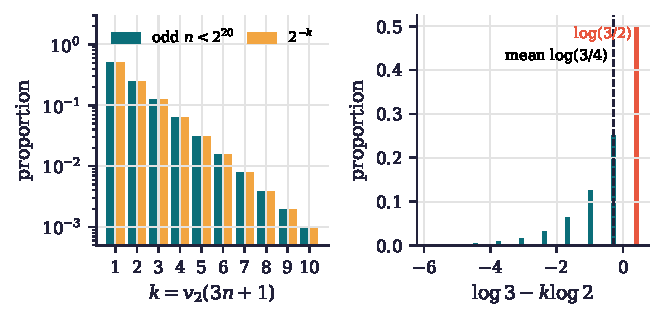
\includegraphics[width=\textwidth]{figures/ch2_syracuse.pdf}
\caption{Left: the proportion of odd $n<2^{20}$ with $\vt(3n+1)=k$ (dark bars) against the Geometric probabilities $2^{-k}$ (light bars); they agree exactly. Right: the induced law of $\log3-k\log2$, the multiplicative part of the Syracuse increment, with the single ascending value $\log(3/2)$, the only bar right of zero, and the mean $\log(3/4)$ dashed.}
\label{fig:ch2:syracuse}
\end{figure}

\begin{remark}[What the Geometric law does not say]\label{rem:ch2:notorbit}
\Cref{prop:geom} describes one Syracuse step from a random odd residue. Along
a single orbit the successive exponents $k_1,k_2,\ldots$ are deterministic.
Along an orbit that reaches $1$ they are eventually all equal to $2$, since $S(1)=1$; along a cycle with $r$ odd values and $s$ halvings in a period their running averages tend to $s/r$, which lies strictly between $\lt$ and $2$ unless the cycle is that of $1$ (summing \eqref{eq:ch2:stride} around the cycle gives $s\log2=\sum\log(3+1/y)$, a sum of $r$ terms in $(\log3,\log4]$, with $\log4$ only at $y=1$); and along a divergent orbit their upper limit is at most $\lt$ (\cref{cor:ch9:freq}).
So whether the running averages tend to $2$ along every orbit is the whole conjecture, and whether their lower limit exceeds $\lt$ along every orbit is exactly the divergence half (\cref{conj:cesaro}).
Taking logarithms in the
Syracuse orbit $x_t=S^{(t)}(n)$,
\[
  \log x_t=\log n+t\log3-(k_1+\cdots+k_t)\log2+\sum_{s<t}\log\Bigl(1+\frac1{3x_s}\Bigr),
\]
so an orbit along which $(k_1+\cdots+k_t)/t$ stays above $\lt+\varepsilon$ for
all large $t$ is bounded. \Cref{chap:divergence} studies this criterion and
its limitations.
\end{remark}

\section{The $2$ adic extension and the shift}\label{sec:ch2:adic}

\Cref{thm:terras} is a statement about every power of $2$ at once, and the
natural setting for such statements is the ring $\Ztwo$ of $2$ adic integers.
We recall what we need. Every $x\in\Ztwo$ has a unique expansion
$x=\sum_{i\geq0}x_i2^i$ with $x_i\in\{0,1\}$; the integers sit inside $\Ztwo$
(negative integers\index{negative cycles} having expansions with infinitely many ones, for instance
$-1=\sum_{i\geq0}2^i$), and so does every rational number with odd
denominator. The $2$ adic absolute value is $|x|_2=2^{-\vt(x)}$, and the balls
$a+2^k\Ztwo$ are both open and closed. Odd integers, and in particular $3$,
are units of $\Ztwo$. The Haar probability measure $\mu$ on $\Ztwo$ is the
unique Borel probability measure invariant under translation; it gives every
ball $a+2^k\Ztwo$ mass $2^{-k}$, and under $\mu$ the digits $x_0,x_1,\ldots$
are independent fair bits.

The accelerated map\index{accelerated map} extends to $\Ztwo$ by the same formula,
\[
  T(x)=\begin{cases}x/2,& x\in2\Ztwo,\\ (3x+1)/2,& x\notin2\Ztwo,\end{cases}
\]
and \cref{lem:ch2:perturb} holds verbatim for $x,a\in\Ztwo$, with the same
proof. Let $\Sigma=\{0,1\}^{\{0,1,2,\ldots\}}$ be the space of infinite binary
sequences with the shift $\mathrm{sh}(w_0,w_1,\ldots)=(w_1,w_2,\ldots)$, the metric
$d(w,w')=2^{-\min\{i:w_i\neq w'_i\}}$, and the Bernoulli product measure
$\beta$ under which the coordinates are independent fair bits. Define the
\emph{parity vector\index{parity vector} map}
\[
  Q:\Ztwo\to\Sigma,\qquad Q(x)=\bigl(T^{(i)}(x)\bmod2\bigr)_{i\geq0}.
\]

\begin{theorem}[Conjugacy to the shift]\label{thm:ch2:conj}
The map $Q$ has the following properties.
\begin{enumerate}[label=(\roman*),leftmargin=2em]
\item $Q$ is a bijective isometry from $(\Ztwo,|\cdot|_2)$ onto $(\Sigma,d)$.
\item $Q\circ T=\mathrm{sh}\circ Q$.
\item $Q$ carries the Haar measure $\mu$ to the Bernoulli measure $\beta$.
\item If $w\in\Sigma$ has ones at positions $d_1<d_2<\cdots$ (finitely or
  infinitely many), then
  \[
    Q^{-1}(w)=-\sum_{j\geq1}3^{-j}2^{d_j},
  \]
  the series converging in $\Ztwo$.
\end{enumerate}
\end{theorem}

The conjugacy (i) to (iii) was first stated explicitly by Lagarias\index{Lagarias, J. C.}~\cite[Theorem~L]{lagarias1985}, who records that it had been observed by Terras\index{Terras, R.} and Pomerance\index{Pomerance, C.}; it rests on the bijection of Terras~\cite{terras1976} and Everett\index{Everett, C. J.}~\cite{everett1977}.
The explicit inverse (iv) is due to
Bernstein\index{Bernstein, D. J.}~\cite{bernstein1994}. Since each part follows in a few lines from
what we have proved, we include the proofs.

\begin{proof}
(i) Let $x\neq y$ in $\Ztwo$ with $|x-y|_2=2^{-j}$, so $y=x+2^ja$ with $a$ a
unit. By \cref{lem:ch2:perturb}, $T^{(i)}(x)$ and $T^{(i)}(y)$ have the same
parity for $i<j$, while $T^{(j)}(y)-T^{(j)}(x)=3^{m_j(x)}a$ is a unit, so the
parities differ at $i=j$. Hence $d(Q(x),Q(y))=2^{-j}=|x-y|_2$. An isometry is
injective and continuous. For surjectivity, let $w\in\Sigma$. By
\cref{thm:terras} there is for each $k$ a unique residue $r_k\bmod2^k$ with
$v_k(r_k)=(w_0,\ldots,w_{k-1})$; since $v_k$ of a residue modulo $2^{k+1}$ is
the truncation of its $v_{k+1}$, we have $r_{k+1}\equiv r_k\pmod{2^k}$. The
compatible residues define $x\in\Ztwo$ with $x\equiv r_k\pmod{2^k}$ for all
$k$, and then the first $k$ entries of $Q(x)$ are $v_k(r_k)$, so $Q(x)=w$.

(ii) The $i$th entry of $Q(T(x))$ is the parity of $T^{(i+1)}(x)$, which is the
$(i+1)$st entry of $Q(x)$.

(iii) By (i), $Q$ maps each ball $x+2^k\Ztwo$ onto the cylinder of sequences
beginning with $v_k(x)$. Both have mass $2^{-k}$, under $\mu$ and $\beta$
respectively. Cylinders form a $\pi$ system generating the Borel
$\sigma$ algebra of $\Sigma$, so the probability measures $\beta$ and
$\mu\circ Q^{-1}$, which agree on cylinders, are equal.

(iv) Let $x=Q^{-1}(w)$. Reducing \eqref{eq:ch2:affine} modulo $2^k$ in $\Ztwo$
gives, as in \cref{cor:ch2:inverse},
$x\equiv-\sum_{j\leq m_k(x)}3^{-j}2^{d_j}\pmod{2^k}$. If $w$ has infinitely
many ones the terms satisfy $|3^{-j}2^{d_j}|_2=2^{-d_j}\to0$, so the series
converges; if finitely many, it is a finite sum. Letting $k\to\infty$ gives the
formula.
\end{proof}

\begin{figure}[ht]
\centering
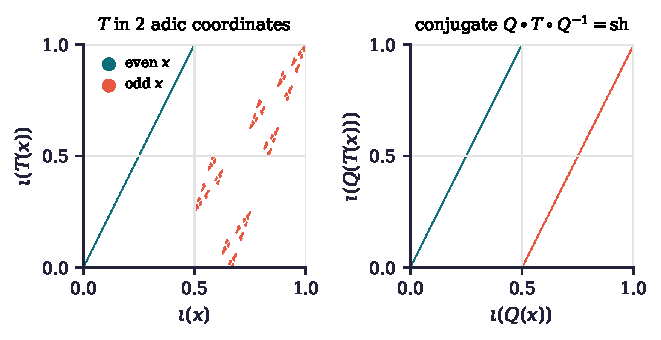
\includegraphics[width=\textwidth]{figures/ch2_adic_shift.pdf}
\caption{The conjugacy of \cref{thm:ch2:conj}, drawn on the residues modulo $2^{16}$. Left: the graph of $T$ in $2$ adic coordinates, a point $x=\sum x_i2^i$ being placed at $\iota(x)=\sum x_i2^{-i-1}\in[0,1)$; even points lie on one line of slope $2$ and odd points scatter. Right: in the coordinates given by the parity vector $Q$, the same map becomes the doubling map, the shift, with even and odd points on its two branches.}
\label{fig:ch2:adicshift}
\end{figure}

For example, $Q(0)=000\cdots$, and $Q(-1)=111\cdots$ since $T(-1)=-1$; indeed $-\sum_{j\geq1}3^{-j}2^{j-1}=-1$ in $\Ztwo$. Similarly $Q(1)=1010\cdots$, since $1\mapsto2\mapsto1$, and
$-\sum_{j\geq1}3^{-j}4^{j-1}=-\tfrac13(1-\tfrac43)^{-1}=1$, the geometric
series converging $2$ adically because $|4/3|_2=1/4$.

Part (iii) contains a measure preservation statement that we isolate, with a
direct proof that does not use the conjugacy.

\begin{proposition}[Haar measure is invariant]\label{prop:ch2:haar}
For every Borel set $A\subseteq\Ztwo$, $\mu(T^{-1}(A))=\mu(A)$.
\end{proposition}

\begin{proof}
It suffices to check balls $A=a+2^k\Ztwo$, since they form a $\pi$ system
generating the Borel sets. A point $x$ lies in $T^{-1}(A)$ either because $x$
is even and $x/2\in A$, that is $x\in2a+2^{k+1}\Ztwo$, or because $x$ is odd
and $(3x+1)/2\in A$, that is
\[
  x\in3^{-1}(2a-1)+2^{k+1}\Ztwo ,
\]
where we used that $3$ is a unit; the centre $3^{-1}(2a-1)$ is odd, so this
ball consists of odd points. The two balls are disjoint and each has measure
$2^{-k-1}$, so $\mu(T^{-1}(A))=2^{-k}=\mu(A)$.
\end{proof}

Since the Bernoulli shift is mixing\index{mixing}, \cref{thm:ch2:conj} shows that $T$ is a
mixing, in particular ergodic, transformation of $(\Ztwo,\mu)$ (Lagarias~\cite[Theorem~K]{lagarias1985}, as a special case of a result of Matthews\index{Matthews, K. R.} and Watts\index{Watts, A. M.}~\cite{matthews1984}).
This is the
cleanest statement of the randomness of the Collatz map, and it is
simultaneously the cleanest statement of why randomness does not suffice: the
positive integers form a set of Haar measure\index{Haar measure} zero in $\Ztwo$, and ergodic
theory is silent about null sets. Inside $\Ztwo$ the conjecture takes the
following form.

\begin{corollary}\label{cor:ch2:tail}
An integer $n\geq1$ satisfies $T^{(k)}(n)=1$ if and only if $\mathrm{sh}^kQ(n)=1010\cdots$.
Hence the Collatz conjecture\index{Collatz conjecture} is equivalent to the statement that the parity
vector of every positive integer ends in the periodic tail $1010\cdots$.
\end{corollary}

\begin{proof}
By (ii), $\mathrm{sh}^kQ(n)=Q(T^{(k)}(n))$, and by (i) this equals $Q(1)$ if and
only if $T^{(k)}(n)=1$.
\end{proof}

\begin{remark}[Rational points and periodic sequences]\label{rem:ch2:periodic}
If $w$ is eventually periodic, then the series in (iv) is eventually a
geometric series and $Q^{-1}(w)$ is a rational number with odd denominator.
The converse, that $Q$ maps every rational number with odd denominator to an
eventually periodic sequence, is the \emph{periodicity conjecture} of
Lagarias~\cite{lagarias1985,lagarias1990}. It would imply that no orbit of a
positive integer is unbounded: if $Q(n)$ is eventually periodic, say
$\mathrm{sh}^{k+p}Q(n)=\mathrm{sh}^kQ(n)$, then $T^{(k+p)}(n)=T^{(k)}(n)$ by
injectivity of $Q$, and the orbit is eventually periodic.
\end{remark}

\section{Stopping times and the density theorem}\label{sec:ch2:density}

\begin{definition}[Stopping times]\label{def:ch2:stopping}
For $n\geq1$ the \emph{stopping time\index{stopping time}} is
$\sigma(n)=\min\{k\geq1:T^{(k)}(n)<n\}$, with $\sigma(n)=\infty$ if there is no
such $k$. The \emph{coefficient stopping time\index{coefficient stopping time}} is
\[
  \tau(n)=\min\{k\geq1:3^{m_k(n)}<2^k\},
\]
the first time the multiplicative coefficient in \eqref{eq:ch2:affine} drops
below $1$.
\end{definition}

If every $n\geq2$ has finite stopping time then the conjecture follows by
strong induction, since the orbit of $n$ reaches a smaller value whose orbit
reaches $1$. Conversely, under the conjecture every $n\geq2$ has finite
stopping time. Note that $\sigma(1)=\infty$ trivially, because the orbit of $1$
never goes below $1$. The coefficient stopping time is a function of the
parity vector\index{parity vector} alone, and therefore of a residue class: if $\tau(n)=k$ then
$\tau(n')=k$ for every $n'\equiv n\pmod{2^k}$.

The following facts, and the exact counts of \cref{sec:ch2:dp}, are due to Terras\index{Terras, R.}~\cite{terras1976} (his Proposition~1.8 and Theorems~1.9, 1.14 and~2.1); see also \cite[Theorem~C]{lagarias1985}.

\begin{proposition}[Stopping times and coefficient stopping times]\label{prop:ch2:tau}
\leavevmode
\begin{enumerate}[label=(\roman*),leftmargin=2em]
\item $\tau(n)\leq\sigma(n)$ for every $n\geq1$.
\item If $\tau(n)=k$ and $m=m_k(n)$, then $\sigma(n')=k$ for every
  $n'\equiv n\pmod{2^k}$ with $n'>c_k(n)/(2^k-3^m)$.
\item If $\tau(n)<\infty$, then $\tau(n)=\lfloor m\lt\rfloor+1$ with
  $m=m_{\tau(n)}(n)$, and the last entry of $v_{\tau(n)}(n)$ is $0$.
\end{enumerate}
\end{proposition}

\begin{proof}
(i) If $T^{(k)}(n)<n$ then by \eqref{eq:ch2:affine}
$3^{m_k}n+c_k=2^kT^{(k)}(n)<2^kn$, and since $c_k\geq0$ this forces
$3^{m_k}<2^k$. So $\tau(n)\leq k$ for every such $k$.

(ii) For $n'$ in the class, $\tau(n')=k$ and $c_k(n')=c_k(n)$, so
$T^{(k)}(n')<n'$ if and only if $3^mn'+c_k(n)<2^kn'$, which is the stated
condition. Then $\sigma(n')\leq k$, and $\sigma(n')\geq\tau(n')=k$ by (i).

(iii) Let $k=\tau(n)<\infty$ and $m=m_k(n)$. If $k=1$ then $n$ is even, $m=0$ and
$k=\lfloor0\rfloor+1$. If $k\geq2$ then $3^{m_{k-1}}\geq2^{k-1}$, and in fact
$3^{m_{k-1}}>2^{k-1}$ since a power of $3$ equals a power of $2$ only when
both are $1$. If the last step were odd we would have $m=m_{k-1}+1$ and
$3^m>3\cdot2^{k-1}>2^k$, contradicting $3^m<2^k$. So the last step is even,
$m=m_{k-1}$, and $2^{k-1}<3^m<2^k$, which says $k-1<m\lt<k$, that is
$k=\lfloor m\lt\rfloor+1$.
\end{proof}

By (iii), finite coefficient stopping times can take only the values $1$, $2$, $4$, $5$, $7$,
$8$, $10$, $12$, $13$, $15$, $16$, $18$, $20$, and so on; the gaps at $3$,
$6$, $9$, $11$, $14$, $17$, $19$, and so on, are the integers
not of the form $\lfloor m\lt\rfloor+1$. By (ii) the same restriction applies
to $\sigma(n)$ for all sufficiently large $n$ in each class with finite $\tau$,
and \cref{prop:ch2:dp} below shows that every value in the list is actually
taken by some residue class.

\begin{example}\label{ex:ch2:stop}
Even $n$ have $\sigma(n)=1$. If $n\equiv1\pmod4$ then the parity vector of length $2$ is $(1,0)$, so
$\tau(n)=2$, $c_2=1$, and $T^{(2)}(n)=(3n+1)/4<n$ for all $n>1$. If
$n\equiv3\pmod{16}$ then $v_4(n)=(1,1,0,0)$, so $m=2$, $c_4=3+2=5$,
$2^4-3^2=7$, and $T^{(4)}(n)=(9n+5)/16<n$ for every $n\geq1$ in the class. In
the other classes modulo $16$, namely $7,11,15\pmod{16}$, the first four
steps do not yet decide.
\end{example}

\Cref{fig:ch2:stopheat} shows the same phenomenon on actual integers. The
stopping times $\sigma(n)$ of $2\leq n<2^{13}$ are arranged in rows of $64$,
so that each column is a residue class modulo $64$. In $56$ of the $64$
columns the stopping time is constant: it is the coefficient stopping time
of the class, reached within six steps. The remaining eight columns are the
classes modulo $64$ whose first six parities do not yet decide, and only there
does the stopping time vary from row to row.

\begin{figure}[t]
\centering
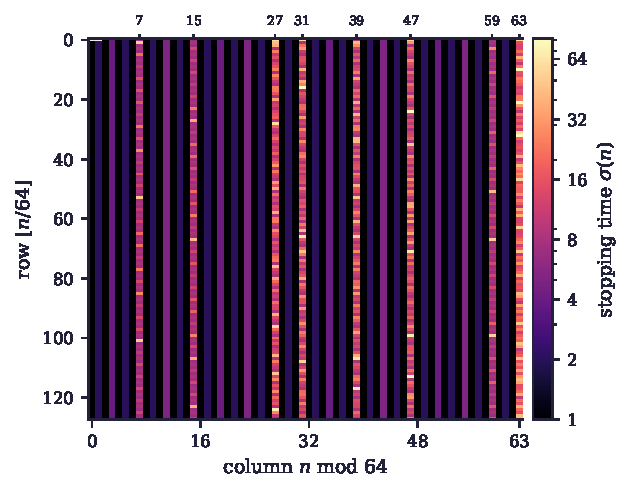
\includegraphics[width=\textwidth]{figures/ch2_stopheat.pdf}
\caption{Stopping times $\sigma(n)$ for $2\leq n<2^{13}$, arranged with $n$ in
row $\lfloor n/64\rfloor$ and column $n\bmod64$, on a logarithmic colour
scale ($n=0,1$ are left blank). Fifty six columns are constant, because
$\tau\leq6$ on them and $\sigma=\tau$ there; the eight columns $7$, $15$,
$27$, $31$, $39$, $47$, $59$, $63$ marked at the top are the classes with
$\tau>6$, a proportion $1/8$ of all classes.}
\label{fig:ch2:stopheat}
\end{figure}

\subsection{Exact counts}\label{sec:ch2:dp}

The number of residue classes that stop at each step can be computed exactly,
without enumerating residues, by a dynamic programme over the number of odd
steps. Call a word $w\in\{0,1\}^k$ \emph{alive} if $3^{m_j(w)}>2^j$ for
$1\leq j\leq k$, where $m_j(w)$ is the number of ones among its first $j$
letters; by \cref{thm:terras} the alive words of length $k$ are the parity
vectors of the residue classes modulo $2^k$ with $\tau>k$. (Since a power of
$3$ never equals a positive power of $2$, the alternative to alive is
$3^{m_j}<2^j$ for some $j$.) Write
\begin{gather*}
  N_k(m)=\#\{w\in\{0,1\}^k\text{ alive}:m_k(w)=m\},\\
  R_k=\#\{r\bmod2^k:\tau(r)=k\}.
\end{gather*}

\begin{proposition}[Exact stopping counts]\label{prop:ch2:dp}
\leavevmode
\begin{enumerate}[label=(\roman*),leftmargin=2em]
\item $N_0(0)=1$, and for $k\geq1$ and $m\geq0$,
  \[
    N_k(m)=\bigl(N_{k-1}(m)+N_{k-1}(m-1)\bigr)\,[\,3^m>2^k\,],
  \]
  with $N_{k-1}(-1)=0$, where $[P]$ is $1$ if $P$ holds and $0$ otherwise. The
  proportion of residues modulo $2^k$ with $\tau>k$
  is $1-F(k)=2^{-k}\sum_mN_k(m)$, and among them the number of odd steps
  in the first $k$ has the law $m\mapsto N_k(m)/\sum_{m'}N_k(m')$.
\item There is at most one integer $m^\ast_k\geq0$ with $2^{k-1}\leq3^{m^\ast_k}<2^k$; equality on the left occurs only for $k=1$ and $m^\ast_1=0$.
  If it exists then $R_k=N_{k-1}(m^\ast_k)\geq1$, and otherwise $R_k=0$.
  Consequently $R_k>0$ if and only if $k=\lfloor m\lt\rfloor+1$ for some
  integer $m\geq0$.
\item The counts satisfy $2^k\bigl(1-F(k)\bigr)=2^{k}\bigl(1-F(k-1)\bigr)-R_k$
  and $F(k)=\sum_{j\leq k}R_j2^{-j}$.
\end{enumerate}
\end{proposition}

\begin{proof}
(i) A word of length $k$ is alive exactly when its prefix of length $k-1$ is
alive and $3^{m_k}>2^k$. Splitting according to the last letter, which is $0$
or $1$, gives the recursion. The statements about residues follow from
\cref{thm:terras}, which makes the parity vector\index{parity vector} of a uniform residue modulo
$2^k$ uniform on $\{0,1\}^k$.

(ii) The condition $2^{k-1}\leq3^m<2^k$ says that $m$ lies in the half open
interval $\bigl[(k-1)/\lt,\,k/\lt\bigr)$, of length $1/\lt<1$, so it has at
most one solution. A residue has $\tau=k$ exactly when its parity word of
length $k$ has an alive prefix of length $k-1$ and $3^{m_k}<2^k$. By
\cref{prop:ch2:tau}(iii) its last letter is then $0$ and $m=m_{k-1}=m_k$
satisfies $2^{k-1}\leq3^m<2^k$ (for $k=1$ the word is $0$ and $m=0$), so $m=m^\ast_k$. Conversely, every alive word of
length $k-1$ with $m^\ast_k$ ones, followed by a $0$, has $\tau=k$. Hence
$R_k=N_{k-1}(m^\ast_k)$. The word $1^{m}0^{k-1-m}$ with $m=m^\ast_k$ is alive,
since $3^{j}>2^{j}$ for $1\leq j\leq m$ and $3^m>2^{j}$ for $m<j\leq k-1$, so $R_k\geq1$. Finally
$m^\ast_k$ exists if and only if $k-1\leq m\lt<k$ for some integer $m\geq0$, that is,
$k=\lfloor m\lt\rfloor+1$.

(iii) Each alive word of length $k-1$ has two extensions, and exactly the
$R_k$ extensions counted in (ii) fail to be alive. The second identity
follows by summing.
\end{proof}

\Cref{tab:ch2:residues} lists $R_k$ and $1-F(k)$ for $k\leq40$, computed
from the recursion with exact integer arithmetic, and \cref{fig:ch2:tree}
draws the first seven levels as a tree. For small $k$ the classes are easily
listed: $\tau=1$ on $0\bmod2$, $\tau=2$ on $1\bmod4$, $\tau=4$ on $3\bmod16$,
$\tau=5$ on $11$ and $23\bmod32$, $\tau=7$ on $7$, $15$ and $59\bmod128$, and
$\tau=8$ on $39$, $79$, $95$, $123$, $175$, $199$ and $219\bmod256$. The
recursion has been checked against direct enumeration of all residues for
$k\leq20$, and the equivalence in (ii) against the recursion for $k\leq400$
(script \texttt{ch02\_exact.py}). \Cref{fig:ch2:sunburst} displays the whole
alive tree to depth nine, coloured by the height $m_k\log3-k\log2$, the
logarithm of the coefficient $3^{m_k}/2^k$ in \eqref{eq:ch2:affine}; a class
stops at the first ring where its height becomes negative.

\begin{table}[t]
\centering
\caption{Number $R_k$ of residue classes modulo $2^k$ with coefficient
stopping time $\tau=k$, and the proportion $1-F(k)$ of residues modulo $2^k$
with $\tau>k$, from \cref{prop:ch2:dp}. The rows with $R_k=0$ are the $k$
not of the form $\lfloor m\lt\rfloor+1$.
Terras~\cite{terras1976} tabulates the same distribution to $k=900$ (his Table~A).}
\label{tab:ch2:residues}
\small\setlength{\tabcolsep}{5pt}
\begin{tabular}{@{}rrr@{\hspace{14pt}}rrr@{}}
\toprule
$k$ & $R_k$ & $1-F(k)$ & $k$ & $R_k$ & $1-F(k)$\\
\midrule
$1$ & $1$ & $0.500000$ & $21$ & $8045$ & $0.022226$\\
$2$ & $1$ & $0.250000$ & $22$ & $0$ & $0.022226$\\
$3$ & $0$ & $0.250000$ & $23$ & $17\,637$ & $0.020123$\\
$4$ & $1$ & $0.187500$ & $24$ & $51\,033$ & $0.017082$\\
$5$ & $2$ & $0.125000$ & $25$ & $0$ & $0.017082$\\
$6$ & $0$ & $0.125000$ & $26$ & $108\,950$ & $0.015458$\\
$7$ & $3$ & $0.101562$ & $27$ & $312\,455$ & $0.013130$\\
$8$ & $7$ & $0.074219$ & $28$ & $0$ & $0.013130$\\
$9$ & $0$ & $0.074219$ & $29$ & $663\,535$ & $0.011894$\\
$10$ & $12$ & $0.062500$ & $30$ & $0$ & $0.011894$\\
$11$ & $0$ & $0.062500$ & $31$ & $1\,900\,470$ & $0.011009$\\
$12$ & $30$ & $0.055176$ & $32$ & $5\,936\,673$ & $0.009627$\\
$13$ & $85$ & $0.044800$ & $33$ & $0$ & $0.009627$\\
$14$ & $0$ & $0.044800$ & $34$ & $13\,472\,296$ & $0.008843$\\
$15$ & $173$ & $0.039520$ & $35$ & $39\,993\,895$ & $0.007679$\\
$16$ & $476$ & $0.032257$ & $36$ & $0$ & $0.007679$\\
$17$ & $0$ & $0.032257$ & $37$ & $87\,986\,917$ & $0.007039$\\
$18$ & $961$ & $0.028591$ & $38$ & $0$ & $0.007039$\\
$19$ & $0$ & $0.028591$ & $39$ & $257\,978\,502$ & $0.006569$\\
$20$ & $2652$ & $0.026062$ & $40$ & $820\,236\,724$ & $0.005823$\\
\bottomrule
\end{tabular}
\end{table}

\begin{figure}[tp]
\centering
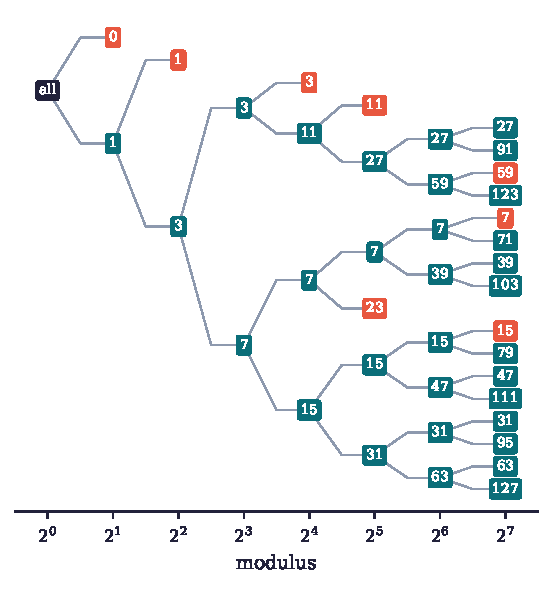
\includegraphics[width=\textwidth]{figures/ch2_residue_tree.pdf}
\caption{The stopping tree. A node at modulus $2^j$ is a residue class modulo $2^j$ whose orbit has not stopped before step $j$. Lighter nodes stop at step $j$ ($\tau=j$) and are leaves; each darker node $r$ splits into the classes $r$ and $r+2^j$ modulo $2^{j+1}$. At modulus $2^7$, $13$ of the $128$ classes remain.}
\label{fig:ch2:tree}
\end{figure}

\begin{figure}[tp]
\centering
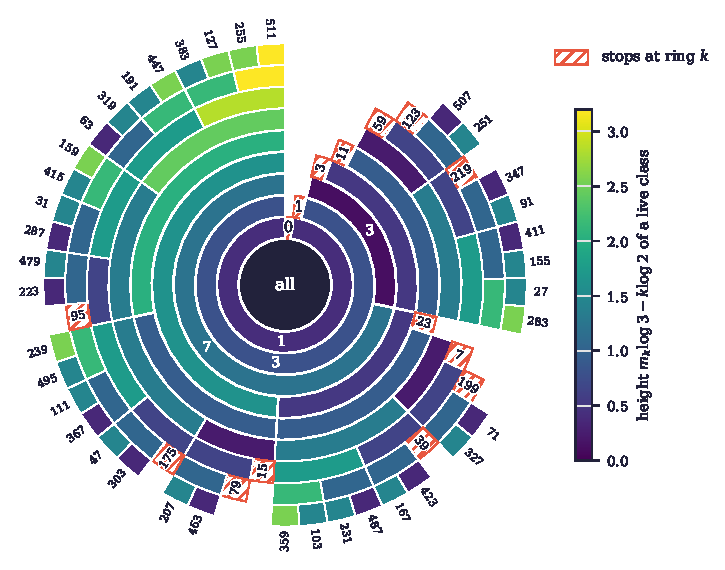
\includegraphics[width=\textwidth]{figures/ch2_sunburst.pdf}
\caption{The Terras parity tree as a sunburst. Ring $k$ consists of residue classes modulo $2^k$, equivalently parity words of length $k$, and the two children of a class in ring $k+1$ are its two lifts. A class that stops at ring $k$ ($\tau=k$) is a hatched wedge labelled by its residue with nothing outside it; live classes are shaded by their height $m_k\log3-k\log2$. Angular width is proportional to the number of leaves below a node, not to Haar measure. The outer labels are the $38$ classes modulo $2^9$ with $\tau>9$.}
\label{fig:ch2:sunburst}
\end{figure}

We can now prove the theorem of Terras\index{Terras, R.} and Everett\index{Everett, C. J.}, in the quantitative form given by Lagarias\index{Lagarias, J. C.}~\cite[Theorem~D]{lagarias1985}.
Write
\[
  F(k)=2^{-k}\,\#\{r\bmod2^k:\tau(r)\leq k\},\qquad
  \theta=\frac{\log2}{\log3}\approx0.6309,
\]
and let
\[
  D=\theta\log(2\theta)+(1-\theta)\log\bigl(2(1-\theta)\bigr)\approx0.03469
\]
be the Kullback\index{Kullback and Leibler divergence} and Leibler divergence of the Bernoulli$(\theta)$ law from the
Bernoulli$(\tfrac12)$ law.
(In this section only, $\theta$ denotes $1/\lt$, the threshold frequency of odd steps; in \cref{chap:cycles} it denotes $\lt$ itself.)

\begin{theorem}[{Terras~\cite{terras1976,terras1979}, Everett~\cite{everett1977}, Lagarias~\cite[Theorem~D]{lagarias1985}}]\label{thm:density}
For each $k\geq1$ the set $\{n\geq1:\sigma(n)\leq k\}$ has natural density
$F(k)$, and
\[
  1-F(k)\leq e^{-Dk}.
\]
Consequently the set of $n\geq1$ with finite stopping time\index{stopping time} has natural
density $1$.
\end{theorem}

\begin{proof}
\emph{Step 1: the coefficient stopping time\index{coefficient stopping time}.} The set $A_k=\{n\geq1:
\tau(n)\leq k\}$ is a union of residue classes modulo $2^k$: whether
$\tau(n)\leq k$ is decided by $v_k(n)$, hence by $n\bmod2^k$. A union of $R$
classes modulo $2^k$ has natural density $R/2^k$, so $A_k$ has density $F(k)$.

\emph{Step 2: comparison with the stopping time.} Let $B_k=\{n\geq1:
\sigma(n)\leq k\}$. By \cref{prop:ch2:tau}(i), $B_k\subseteq A_k$. Conversely,
each class $r\bmod2^j$ with $\tau=j\leq k$ is contained in $B_k$ apart from the
finitely many $n\leq c_j(r)/(2^j-3^{m_j(r)})$, by \cref{prop:ch2:tau}(ii). There
are finitely many such classes, so $A_k\setminus B_k$ is finite, and $B_k$ has
the same density $F(k)$ as $A_k$.

\emph{Step 3: reduction to a binomial tail.} By \cref{cor:ch2:iid}, $1-F(k)$
is the probability that a uniformly random word $w\in\{0,1\}^k$ satisfies
$3^{m_j(w)}\geq2^j$ for every $j\leq k$, where $m_j(w)$ is the number of ones
among the first $j$ letters. In particular such a word has $3^{m_k(w)}\geq2^k$,
that is $m_k(w)\geq\theta k$. Hence
\[
  1-F(k)\leq\Prob(X\geq\theta k),\qquad X\sim\mathrm{Binomial}(k,\tfrac12).
\]

\emph{Step 4: the Chernoff\index{large deviations} bound.} For every $\lambda>0$, Markov's inequality
applied to $e^{\lambda X}$ gives
\[
  \Prob(X\geq\theta k)\leq e^{-\lambda\theta k}\,\E e^{\lambda X}
  =\Bigl(e^{-\lambda\theta}\,\frac{1+e^{\lambda}}{2}\Bigr)^{k}.
\]
Since $\theta>\tfrac12$ we may take $e^{\lambda}=\theta/(1-\theta)>1$. Then
$(1+e^\lambda)/2=1/(2(1-\theta))$ and $e^{-\lambda\theta}=((1-\theta)/\theta)^{\theta}$,
and the logarithm of the bracket is
\begin{align*}
  -\theta\log\frac{\theta}{1-\theta}&-\log\bigl(2(1-\theta)\bigr)\\
  &=-\theta\log(2\theta)-(1-\theta)\log\bigl(2(1-\theta)\bigr)=-D .
\end{align*}
So $1-F(k)\leq e^{-Dk}$.

\emph{Step 5: conclusion.} The set $B=\{n:\sigma(n)<\infty\}$ contains $B_k$
for every $k$, so its lower density is at least $F(k)\geq1-e^{-Dk}$ for every
$k$. Since $D>0$, the lower density of $B$ is $1$, and hence $B$ has natural
density $1$.
\end{proof}

\begin{figure}[tp]
\centering
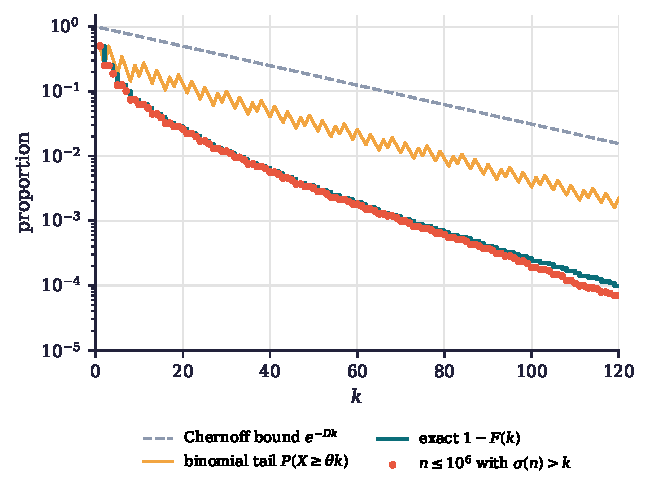
\includegraphics[width=\textwidth]{figures/ch2_stopdecay.pdf}
\caption{Decay of the proportion of residues that have not stopped. Dark solid line: the exact density $1-F(k)$ of $\{\tau>k\}$. Dots: the fraction of $n\leq10^6$ with $\sigma(n)>k$. Light solid line: the binomial tail used in Step 3 of the proof. Dashed line: the Chernoff bound $e^{-Dk}$.}
\label{fig:ch2:stopdecay}
\end{figure}

\Cref{fig:ch2:stopdecay} compares the exact proportion $1-F(k)$, computed by
dynamic programming over the number of ones in the parity word, with the
bounds used in the proof. The bound is valid but loose: at $k=100$ the exact
value is $2.39\times10^{-4}$, the binomial tail is $3.32\times10^{-3}$, and the
Chernoff bound is $3.12\times10^{-2}$. The ratio $(1-F(k))/e^{-Dk}$ falls
from $0.052$ at $k=20$ to $0.0077$ at $k=100$ and $0.0032$ at $k=200$. Step 3
throws away the requirement that the walk $j\mapsto m_j\log3-j\log2$ stay
nonnegative at every intermediate time and keeps only the endpoint.
This loses at most a factor $k$ (\cref{ex:ch2:sharp}), so the exponent $D$ cannot be improved, as Lagarias\index{Lagarias, J. C.}~\cite{lagarias1985} observes.
The endpoint probability is of order $k^{-1/2}e^{-Dk}$, and for a random walk with negative drift\index{drift} the probability of staying above a barrier for $k$ steps is, heuristically, smaller by a further factor of order $k^{-1}$, so of order $k^{-3/2}e^{-Dk}$.
The local exponent of the observed ratio to $e^{-Dk}$, $-1.19$ between $k=20$ and $k=100$ and $-1.41$ between $k=400$ and $k=800$, approaches $-3/2$ slowly; we do not need or prove this refinement.

Two further remarks place the theorem in context.

\begin{remark}[The coefficient stopping time conjecture]\label{rem:ch2:cst}
We always have $\tau\leq\sigma$ by \cref{prop:ch2:tau}, with equality
for all sufficiently large members of each class.
Terras~\cite{terras1976} conjectured that every $n\geq2$ has $\sigma(n)=\tau(n)$, verified this for $n<250\,000$, and deduced from an explicit bound that it holds for every $n$ with $\tau(n)<2592$; see Lagarias\index{Lagarias, J. C.}~\cite[Theorem~H]{lagarias1985}.
We have also checked it directly for $2\leq n\leq10^6$.
The
conjecture would rule out nontrivial cycles: if $n\geq2$ were the least
element of a cycle of length $k$ with $m$ odd elements, then $\sigma(n)=\infty$,
while $3^m<2^k$ by \cref{cor:ch2:cycle}, so $\tau(n)\leq k$. It says nothing
directly about unbounded orbits, since a starting value of such an orbit
could have $\tau=\infty$ as well. Among
$n\leq10^6$ the largest stopping time is $\sigma(626\,331)=176$; half of all
$n$ have $\sigma(n)=1$ and a quarter have $\sigma(n)=2$, in agreement with
\cref{tab:ch2:residues}.
\end{remark}

\begin{remark}[Why density one is not enough]\label{rem:ch2:notenough}
\Cref{thm:density} says that almost every $n$ falls below itself. It does not
say that almost every $n$ reaches $1$. To descend from $n$ to $1$ an orbit
must pass through a chain of smaller values each of which must itself have
finite stopping time, and the exceptional set, though of density zero, might
contain a value on every orbit. Repeating the argument from the value
$T^{(\sigma(n))}(n)$ is not legitimate, because that value is not uniformly
distributed in any residue class: it is determined by $n$, and its residues
have been used up in computing $\sigma(n)$. This is the gap between ensemble
and orbit that recurs throughout the book. Results that go further, from
Korec\index{Korec, I.}'s exponent $\log3/\log4$ to Tao\index{Tao, T.}'s almost bounded values, are described
in \cref{chap:intro}.
\end{remark}

\section*{Notes}

The parity vector\index{parity vector} and its bijection with residues are due to
Terras\index{Terras, R.}~\cite{terras1976} and Everett\index{Everett, C. J.}~\cite{everett1977}; see \cite[Theorem~B]{lagarias1985}.
Terras also introduced the coefficient stopping time\index{coefficient stopping time}\index{stopping time}, proved the facts collected in \cref{prop:ch2:tau}, gave the recursion of \cref{prop:ch2:dp} with a table of the resulting distribution (his Table~A) and the description of the values of $\tau$ with a table of them (his Table~B), proved that the limiting distribution $F(k)$ exists, as in Steps 1 and 2 of the proof of \cref{thm:density}, and, by the central limit theorem, that $F(k)\to1$, which is the density statement of \cref{thm:density} (further details of the proof are in a later note~\cite{terras1979}), and stated the coefficient stopping time conjecture.
The density
statement was proved independently by Everett~\cite{everett1977}, who worked
with $f(2n)=n$, $f(2n+1)=3n+2$, which is our accelerated map\index{accelerated map} $T$.
The exponential bound of \cref{thm:density} is Theorem~D of Lagarias\index{Lagarias, J. C.}~\cite{lagarias1985}, proved there by bounding the same binomial tail; Lagarias also observes that its exponent cannot be improved.
The survey of
Lagarias\index{Lagarias, J. C.}~\cite{lagarias1985} gives a unified account of these results, the
$2$ adic extension and the conjugacy of \cref{thm:ch2:conj}, and many
generalizations; its section on the $2$ adic viewpoint is still the best
introduction. Bernstein\index{Bernstein, D. J.}~\cite{bernstein1994} gave the noniterative formula
for $Q^{-1}$, and the rational cycles\index{rational cycles} of the extended map are studied by
Lagarias~\cite{lagarias1990}. Wirsching\index{Wirsching, G. J.}~\cite{wirsching1998} develops the
combinatorics of parity words and of the inverse tree\index{inverse tree} in depth.
The identity $T^{(j)}(2^ja-1)=3^ja-1$ of \cref{rem:ch2:pitfall} is classical; see
Hercher\index{Hercher, C.}~\cite[Lemma~8]{hercher2023}, who cites Terras~\cite{terras1976} for it.

The affine identity \eqref{eq:ch2:affine} and the cycle formula
\eqref{eq:ch2:cyclen} are classical and appear, in various notations, in most
treatments of cycles; we have followed the notation of our Lean\index{Lean} formalization,
in which the recursion \eqref{eq:ch2:crec} is the inductive step of the proof.
The sum \eqref{eq:ch2:cexplicit} is a sum of terms $3^j2^i$ indexed by the
parity word, and the question of whether its structure, rather than only its
size, can constrain cycles is one of the open problems of \cref{chap:open}.

The Chernoff\index{large deviations} argument in Step 4 is the simplest route to an explicit rate; the
true asymptotics of $1-F(k)$ are those of the probability that a random walk with negative drift\index{drift} stays positive for $k$ steps.
\Cref{chap:stochastic} recovers the same
exponential rate for the first descent of the stochastic model, though not the
finer asymptotics.

\section*{Exercises}

\begin{exercise}\label{ex:ch2:runs}
Prove the identity $T^{(i)}(2^ja-1)=3^i2^{j-i}a-1$ of \cref{rem:ch2:pitfall}.
Deduce that $T^{(j)}(2^j-1)=3^j-1$, and that for every $j$ there are infinitely
many $n$ whose orbits under $T$ begin with exactly $j$ odd steps followed by an
even step.
\end{exercise}

\begin{exercise}\label{ex:ch2:bernstein}
Use \cref{thm:ch2:conj}(iv) to find the $2$ adic integer whose parity vector\index{parity vector}
is the periodic word $110110\cdots$, and show that it is $-5$. Explain the answer in terms of the cycle
$-5\mapsto-7\mapsto-10\mapsto-5$. More generally, show that if $w$ is periodic
with period $k$ and has $m$ ones in each period, then $Q^{-1}(w)=c(w)/(2^k-3^m)$
with $c(w)$ the sum \eqref{eq:ch2:cexplicit} over one period, in agreement with
\cref{cor:ch2:cycle}.
\end{exercise}

\begin{exercise}\label{ex:ch2:class11}
For $n\equiv11\pmod{32}$ compute $v_5(n)$, $m_5(n)$ and $c_5(n)$, and show that
$T^{(5)}(n)=(27n+23)/32$. Deduce that $\sigma(n)=5$ for every such $n$, and
compute the natural densities of $\{\sigma=4\}$ and $\{\sigma=5\}$.
\end{exercise}

\begin{exercise}\label{ex:ch2:syrhaar}
Let $U=\Ztwo\setminus2\Ztwo$ be the $2$ adic units with normalized Haar measure\index{Haar measure}
$\mu_U=2\mu|_U$, and extend the Syracuse map\index{Syracuse map} to $U\setminus\{-1/3\}$. Show
that for an odd ball $b+2^k\Ztwo$ the preimage under $S$ is the disjoint union
over $j\geq1$ of the balls $3^{-1}(2^jb-1)+2^{k+j}\Ztwo$, and deduce that $S$
preserves $\mu_U$. Show that under $\mu_U$ the halving exponent of $S$ has
exactly the Geometric$(\tfrac12)$ law.
\end{exercise}

\begin{exercise}\label{ex:ch2:sharp}
Let $X$ and $\theta$ be as in the proof of \cref{thm:density}. Let $w\in\{0,1\}^k$ satisfy $3^{m_k(w)}>2^k$, and let $j$ be the last index in $\{0,\ldots,k-1\}$ at which $m_j(w)\log3-j\log2$ is smallest. Show that the word obtained from $w$ by moving its first $j$ letters to the end is alive, in the sense of \cref{sec:ch2:dp}, and deduce that $\Prob(X\geq\theta k)/k\leq1-F(k)\leq\Prob(X\geq\theta k)$. Using $\binom ki\geq2^{kH(i/k)}/(k+1)$, where $H(x)=-x\log_2x-(1-x)\log_2(1-x)$, and $D=(1-H(\theta))\log2$, show that $\frac1k\log\bigl(1-F(k)\bigr)\to-D$, so that the exponent in \cref{thm:density} cannot be improved.
\end{exercise}

\begin{exercise}\label{ex:ch2:standard}
Formulate and prove the analogue of \cref{thm:terras} for the standard map\index{standard map}
$T_0$. Show that the parity vectors of length $k$ under $T_0$ are exactly the
binary words with no two consecutive ones, that their number is the
Fibonacci number $\mathrm{Fib}_{k+2}$ (with $\mathrm{Fib}_1=\mathrm{Fib}_2=1$), and that the set of $n$ with a given word $w$ is a
single residue class modulo $2^{z+1}$, where $z$ is the number of zeros among
the first $k-1$ letters of $w$. Explain why there is no longer a bijection
with the residues modulo a fixed power of $2$.
\end{exercise}

\chapter{Stochastic Models and Martingale Duality}\label{chap:stochastic}

The previous chapter proved that a uniformly random residue modulo $2^k$
produces a parity vector\index{parity vector} of $k$ independent fair coin flips. It is a short
step from this theorem to a model: pretend that the parities along an orbit
are fair coin flips forever, and study the resulting random walk for $\log x$.
The model rests on this theorem of Terras\index{Terras, R.}~\cite{terras1976} and Everett\index{Everett, C. J.}~\cite{everett1977} and was stated as a heuristic by Crandall\index{Crandall, R. E.}~\cite{crandall1978} (\cref{sec:ch3:heuristic} tells its history).
Its predictions agree closely with computation (the fitted slope of the total stopping times to within about two percent over the ranges tested, and to within half a percent for the accelerated map below $10^4$; their variance to about ten percent), and it is the reason almost everyone who has thought about the problem believes the conjecture.

This chapter develops the model with the tools of martingale\index{martingale} theory. The
organizing fact is a duality. Under the fair coin model for the accelerated
map, the iterates $x_n$ themselves form a martingale, because
$\tfrac12\cdot\tfrac12+\tfrac12\cdot\tfrac32=1$ exactly, while their
logarithms form a supermartingale\index{supermartingale} with strictly negative drift\index{drift}
$\ds=\log(\sqrt3/2)\approx-0.1438$. The two statements are reconciled by
Jensen's inequality\index{Jensen inequality}, and the drift is exactly the Jensen gap.
The heuristic is therefore not a statement about the size of the iterates on average, which in the model does not decrease at all, but about the size of their logarithms.
Almost everything else in the chapter follows from this observation: the total stopping
time slope $1/|\ds|\approx6.952$ through Wald's identity\index{Wald identity}, the dispersion of
total stopping times\index{stopping time} through the central limit theorem\index{central limit theorem} and the moment asymptotics for first passage times, a
bound of exactly $1/K$ on the probability of an excursion by a factor $K$
through Ville\index{Ville inequality}'s maximal inequality, absorption with probability one, and the
failure of uniform integrability\index{uniform integrability} that prevents the martingale from saying
anything about where the orbit ends. We also treat the standard map\index{standard map} $T_0$,
whose model parity sequence is not independent but a renewal\index{renewal theory} sequence, and we
compute its autocorrelation\index{autocorrelation} function exactly: $\rho(h)=(-\tfrac12)^h$.

Apart from \cref{prop:ch3:exact,prop:ch3:pathwise}, which are statements about the map, every result in this chapter is a theorem about a probabilistic model, and the
model is not the Collatz map. We say so at the start because the point is easy
to lose in the middle of a computation. The final section asks what a proof of
the conjecture along these lines would have to supply, and the answer, a
certificate\index{certificate} that transfers the model's conclusions to individual orbits, is
the subject of much of the rest of the book.

\section{The parity heuristic}\label{sec:ch3:heuristic}

\subsection{From Terras to Lagarias and Weiss}

Terras\index{Terras, R.}~\cite{terras1976} and, independently, Everett\index{Everett, C. J.}~\cite{everett1977}
introduced the parity vector\index{parity vector} and proved that its first
$k$ entries are uniformly distributed when the starting value is uniformly
distributed modulo $2^k$ (\cref{thm:terras}; see \cite[Theorem~B]{lagarias1985}),
and both proved that almost all integers have a finite stopping time
(the density statement of \cref{thm:density}, whose exponential rate is due to Lagarias\index{Lagarias, J. C.}~\cite[Theorem~D]{lagarias1985}; see also~\cite{terras1979}). Both papers use the coin flip
picture to prove theorems about densities of starting values, and both are
careful to stay within the range of steps that the residue class actually
controls. The heuristic consists in ignoring that limitation.

The heuristic was stated explicitly by Crandall\index{Crandall, R. E.}~\cite{crandall1978}.
Lagarias\index{Lagarias, J. C.}, in his 1985 survey~\cite[\S2.1]{lagarias1985}, recorded it
and pointed out that it predicts the growth rate of total stopping times\index{stopping time}.
Lagarias and Weiss\index{Weiss, A.}~\cite{lagarias1992} then studied two stochastic models in
detail, a random walk model for the trajectory of a single integer and a
branching random walk model for the tree of preimages, and compared their
predictions for total stopping times and maximal excursions with extensive
computation. Kontorovich\index{Kontorovich, A. V.} and Sinai\index{Sinai, Ya. G.}~\cite{kontorovich2002} proved a structure
theorem for a broad family of maps of Collatz type, showing that the
logarithm of a trajectory from a random starting value behaves like a random
walk with drift\index{drift}; and the survey of Kontorovich and
Lagarias~\cite{kontorovich2009} places all of this, together with the $5x+1$
problem, where the drift is positive and orbits are expected to diverge, in a
common framework.

We shall use three versions of the model, one for each of the maps of
\cref{def:maps}. Throughout the chapter the multiplicative factor $3+1/x$ is
replaced by $3$; we comment on this replacement in
\cref{rem:ch3:plusone}.

\begin{definition}[Three stochastic models]\label{def:ch3:models}
\leavevmode
\begin{enumerate}[label=(\alph*),leftmargin=2em]
\item \emph{Bernoulli model for $T$.} Let $\xi_1,\xi_2,\ldots$ be independent
  with $\Prob(\xi_i=\tfrac12)=\Prob(\xi_i=\tfrac32)=\tfrac12$, and put
  $x_n=x_0\xi_1\cdots\xi_n$. The log increments are $\Delta_i=\log\xi_i$, and
  $\Filt_n=\sigma(\xi_1,\ldots,\xi_n)$.
\item \emph{Stride model for $S$.} Let $K_1,K_2,\ldots$ be independent,
  each with the Geometric$(\tfrac12)$ law, so that $\Prob(K_j=k)=2^{-k}$ for
  $k\geq1$, and put $X_j=X_{j-1}\cdot3\cdot2^{-K_j}$.
\item \emph{Renewal model for $T_0$.} Let $(B_n)_{n\geq0}$ be the Markov chain
  on $\{0,1\}$ with transition probabilities
  \begin{gather*}
    \Prob(B_{n+1}=0\mid B_n=1)=1,\\
    \Prob(B_{n+1}=0\mid B_n=0)=\Prob(B_{n+1}=1\mid B_n=0)=\tfrac12,
  \end{gather*}
  and put $x_{n+1}=3x_n$ if $B_n=1$ and $x_{n+1}=x_n/2$ if $B_n=0$. Here
  $B_n$ is the model counterpart of the parity $b_n=T_0^{(n)}(x_0)\bmod2$ of an
  orbit (\cref{prop:nocons}), and $\Filt_n=\sigma(B_0,\ldots,B_n)$.
\end{enumerate}
\end{definition}

The three models are consistent with one another in the same way the three maps
are. In model (c) an odd step is always followed by a halving, by
\cref{prop:nocons}; merging each odd step with the halving that follows it
produces a step with factor $3/2$, and the parity after that is again a fair
coin, so model (c) with the forced steps deleted is model (a). Grouping the
steps of model (a) into runs that begin with a factor $\tfrac32$ and continue
with factors $\tfrac12$ until the next $\tfrac32$ produces the factor
$3\cdot2^{-K}$ with $K$ Geometric$(\tfrac12)$, which is model (b). The three
models therefore describe one random path measured against three clocks, which
tick on average three times, twice and once per stride.

\subsection{In what sense the model is exact}

The model is not an analogy chosen for convenience. Over an initial segment of
the orbit whose length is controlled by the size of the starting residue class
it is exact, up to the replacement of $3+1/x$ by $3$.

\begin{proposition}[Ensemble exactness]\label{prop:ch3:exact}
Let $k\geq1$ and let $n$ be uniformly distributed on a complete set of residues
modulo $2^k$ consisting of positive integers. Then the parities of $T^{(j)}(n)$
for $0\leq j<k$ are independent and fair, and for $j\leq k$
\[
  \log T^{(j)}(n)-\log n=\sum_{i=1}^{j}\Delta_i+\sum_{\substack{0\le i<j\\
  T^{(i)}(n)\ \mathrm{odd}}}\log\Bigl(1+\frac{1}{3T^{(i)}(n)}\Bigr),
\]
where $\Delta_{i+1}=\log\frac32$ if $T^{(i)}(n)$ is odd and $\Delta_{i+1}=-\log2$
otherwise. Thus the first $k$ log increments of $T$ have exactly the joint law
of the increments of the Bernoulli model\index{Bernoulli model}, apart from correction terms that are
positive and at most $1/(3T^{(i)}(n))$ each.
\end{proposition}

\begin{proof}
The first statement is \cref{cor:ch2:iid}. The second is the identity
$T(x)/x=\tfrac32(1+\tfrac1{3x})$ for odd $x$ and $T(x)/x=\tfrac12$ for even
$x$, summed along the orbit.
\end{proof}

\Cref{prop:ch3:exact} is the source of the model's authority and also of its
limitation. A starting value $n$ of size about $2^k$ carries $k$ bits, and the
first $k$ steps of its orbit consume them, one bit per step. After that the
parities are a deterministic function of information that the orbit itself
has generated, and no theorem says that they continue to look like coin flips.
Since an orbit from $n$ needs about $\log n/|\ds|\approx4.8\log_2n$ steps of
$T$ to reach $1$ (\cref{prop:lyapunov}), roughly four fifths of a typical orbit lies beyond the range
where the model is a theorem.

\begin{remark}[The plus one]\label{rem:ch3:plusone}
Replacing $3+1/x$ by $3$ changes each odd step by a factor
$1+1/(3x)$, so the cumulative effect on $\log x$ along an orbit is
at most $\sum1/(3x_i)$ over its odd steps, which is negligible unless the orbit lingers at small
values. The replacement matters in two places only. Near the end of an orbit
it decides whether the path lands on the cycle $1\to2\to1$ under $T$, which the
multiplicative model cannot see. And it is the whole difference between the
$3x+1$ map and its multiplicative caricature, in which an exact return to a
previous value would require $3^m=2^k$; the cycle analysis of
\cref{chap:cycles} lives entirely in the $+1$. For questions of drift\index{drift}, dispersion and excursion, which are the
subject of this chapter, it is harmless.
\end{remark}

\section{Martingale duality}\label{sec:ch3:duality}

We begin with the accelerated map\index{accelerated map}, where the model is simplest.

\begin{proposition}[Martingale duality]\label{thm:martingale}
In the Bernoulli model\index{Bernoulli model} for the accelerated map $T$:
\begin{enumerate}[label=(\roman*),leftmargin=2em]
\item \emph{Multiplicative martingale.} $\E[\xi_i]=\tfrac12\cdot\tfrac12+
  \tfrac12\cdot\tfrac32=1$, so $(x_n)$ is a nonnegative martingale with
  $\E[x_n]=x_0$ for every $n$.
\item \emph{Log supermartingale.} $\E[\Delta_i]=\tfrac12\log\tfrac32-\tfrac12\log2
  =\log\frac{\sqrt3}{2}=\ds\approx-0.1438$, so $(\log x_n)$ is a strict
  supermartingale\index{martingale}\index{supermartingale}, and $\log x_n-n\ds$ is a martingale.
\item \emph{Wald root.} The moment generating function of the increment,
  \[
    M(\theta)=\E\bigl[e^{\theta\Delta_i}\bigr]=\tfrac12\,2^{-\theta}+
    \tfrac12\bigl(\tfrac32\bigr)^{\theta},
  \]
  is strictly convex with $M(0)=M(1)=1$. Its nonzero root
  $\theta^*$ of $M(\theta)=1$ is $\theta^*=1$, and $x_n^{\theta}$ is a
  supermartingale for $0\le\theta\le1$ and a submartingale for $\theta\geq1$
  or $\theta\le0$.
\item \emph{Jensen gap.} $\ds=\E[\log\xi_i]-\log\E[\xi_i]$, so the drift of
  $\log x_n$ is exactly the Jensen defect of the logarithm at the law of
  $\xi_i$.
\end{enumerate}
\end{proposition}

\begin{proof}
Parts (i) and (ii) are the two displayed computations together with the
independence of $\xi_{n+1}$ from $\Filt_n$: $\E[x_{n+1}\mid\Filt_n]=x_n\E[\xi_{n+1}]
=x_n$ and $\E[\log x_{n+1}\mid\Filt_n]=\log x_n+\ds$. For (iii),
$M(0)=1$ and $M(1)=\tfrac14+\tfrac34=1$. Since $M''(\theta)=\E[\Delta^2e^{\theta
\Delta}]>0$, $M$ is strictly convex, so it equals $1$ at exactly two points and
is below $1$ strictly between them and above $1$ outside. Finally
$\E[x_{n+1}^\theta\mid\Filt_n]=x_n^\theta M(\theta)$. Part (iv) restates (ii)
using $\log\E[\xi_i]=0$ from (i).
\end{proof}

Parts (i) and (ii) of \cref{thm:martingale} appear to contradict each other. By (i) the expected size of $x_n$ never
changes. By (ii) and the strong law of large numbers, $\log x_n/n\to\ds<0$
almost surely, so almost every path tends to zero exponentially fast, at the
rate $e^{n\ds}=(\sqrt3/2)^n$. Both are true. The mean is held up by rare paths
that grow enormously, and the typical path has nothing to do with the mean.
This is the familiar behaviour of a product of independent positive factors
with mean one, the same mechanism by which a fair multiplicative bet ruins
almost every gambler while preserving the expected wealth of the population.

\begin{remark}[Size of the Jensen gap]\label{rem:ch3:jensen}
The factor $\xi$ has mean $1$ and variance $\E\xi^2-1=\tfrac12(\tfrac14+\tfrac94)
-1=\tfrac14$. The second order expansion $\E\log\xi\approx\log\E\xi-
\Var(\xi)/(2(\E\xi)^2)$ gives $-\tfrac18=-0.125$, against the exact value
$\ds=-0.1438$.
The two values are symmetric about $1$, so the odd moments of $\xi-1=\pm\tfrac12$ vanish and $\E\log\xi=-\sum_{j\geq1}4^{-j}/(2j)=\tfrac12\log\tfrac34$; the second order value $-\tfrac18$ is the first term of this series, and the difference comes from the higher even moments.
Thus the descent of a Collatz orbit, in the model, is a pure fluctuation
effect. A process with the same mean factor and no fluctuation would neither
rise nor fall. This is why, in the model for $T$, any argument that works with $x_n$ directly, or with
any quantity linear in $x_n$, sees no drift\index{drift} at all; we shall meet the same phenomenon
from the side of majorization\index{majorization} in \cref{chap:lyapunov}, where the linear
majorizer of $\log$ is blind to descent for exactly this reason.
\end{remark}

For a random walk $S_n=\sum_{i\le n}\Delta_i$
with negative drift, the positive root $\theta^*$ of $M(\theta)=1$ governs the
probability of large upward excursions: $e^{\theta^*S_n}$ is a martingale, and
the maximal inequality applied to it gives the Lundberg bound
$\Prob(\sup_nS_n\geq u)\le e^{-\theta^*u}$, as we show in
\cref{sec:ch3:ville}. For the Collatz model the root is $\theta^*=1$ exactly,
which is (i) seen from the other side: $e^{S_n}=x_n/x_0$, so the Wald
martingale is the orbit itself. The same root appears for the stride model,
whose moment generating function $M_S(p)=3^p/(2^{1+p}-1)$ also satisfies
$M_S(1)=1$, as we compute in \eqref{eq:ch4:mgf}. It must: whenever a model makes
the iterates themselves a martingale, the exponential martingale with
parameter one is the identity, and the root is $1$ whatever clock is used.

\section{The standard map and its renewal structure}\label{sec:ch3:standard}

The fair coin heuristic is usually stated for $T$, and there is a good reason.
Applied naively to $T_0$ it gives the wrong sign.

\begin{remark}[A tempting but false argument]\label{rem:ch3:naive}
``Under $T_0$ the parities are fair coins, so with probability $\tfrac12$ a step
multiplies by $3$ and with probability $\tfrac12$ it divides by $2$. The
expected log increment is $\tfrac12\log3-\tfrac12\log2=\tfrac12\log\tfrac32>0$,
so orbits of $T_0$ should grow.'' The error is in the first sentence. Under
$T_0$ an odd step is always followed by an even step (\cref{prop:nocons}), so
the parities are not independent and are not fair: in the long run only one
step in three is odd. The correct computation, in
\cref{prop:ch3:standard} below, gives the drift\index{drift} $\tfrac13\log\tfrac34<0$ per
step.
\end{remark}

The renewal\index{renewal theory} model of \cref{def:ch3:models}(c) encodes the forced halving. Its
transition matrix, with states ordered $(0,1)$ and columns indexed by the
current state, is
\[
  P=\begin{pmatrix}\tfrac12&1\\[2pt]\tfrac12&0\end{pmatrix},
\]
with eigenvalues $1$ and $-\tfrac12$. The eigenvalue $-\tfrac12$ will reappear
as the base of the autocorrelation\index{autocorrelation} function in \cref{sec:ch3:autocorr}.

\begin{proposition}[Martingale structure of the standard map]\label{prop:ch3:standard}
In the renewal model for $T_0$:
\begin{enumerate}[label=(\roman*),leftmargin=2em]
\item The stationary law of the parity chain is $\Prob(B_n=1)=\tfrac13$, and
  the fraction of odd steps among the first $n$ converges to $\tfrac13$
  almost surely from any initial state.
\item $(x_n)$ is not a martingale: $\E[x_{n+1}\mid\Filt_n]=3x_n$ on
  $\{B_n=1\}$. The process $M_n=3^{B_n}x_n$ is a martingale\index{martingale}.
\item $(\log x_n)$ is not a supermartingale, since its increment is $+\log3$
  on $\{B_n=1\}$. The process $\log M_n$ is a supermartingale\index{supermartingale}, with
  conditional drift $0$ on $\{B_n=1\}$ and $\ds$ on $\{B_n=0\}$.
\item Almost surely, $\frac1n\log x_n\to\tfrac13\log3-\tfrac23\log2=
  \tfrac13\log\tfrac34=\tfrac23\ds\approx-0.0959$.
\item Let $\tau_1<\tau_2<\cdots$ be the successive times at which $B_n=1$.
  Then $X_j=x_{\tau_j}$ satisfies $X_{j+1}=3X_j2^{-K_{j+1}}$, where
  $K_{j+1}=\tau_{j+1}-\tau_j-1$ are independent Geometric$(\tfrac12)$, and
  $(X_j)$ is a martingale: $\E[3\cdot2^{-K}]=3\sum_{k\ge1}4^{-k}=1$.
\end{enumerate}
\end{proposition}

\begin{proof}
(i) The stationary vector $\pi$ of $P$ satisfies $\pi_1=\tfrac12\pi_0$ and
$\pi_0+\pi_1=1$, so $\pi_1=\tfrac13$. The chain is irreducible and aperiodic
(state $0$ has a loop), so the ergodic theorem for finite Markov chains gives
the almost sure frequency.

(ii) On $\{B_n=1\}$ we have $x_{n+1}=3x_n$ and $B_{n+1}=0$, so
$M_{n+1}=3x_n=M_n$. On $\{B_n=0\}$ we have $x_{n+1}=x_n/2$ and $B_{n+1}$ is a
fair coin, so $\E[M_{n+1}\mid\Filt_n]=\tfrac{x_n}{2}\cdot\tfrac12(1+3)=x_n=M_n$.

(iii) On $\{B_n=1\}$ the increment $\log M_{n+1}-\log M_n$ is $0$. On
$\{B_n=0\}$ it is $-\log2+B_{n+1}\log3$, with conditional mean
$-\log2+\tfrac12\log3=\ds$.

(iv) $\log x_n=\log x_0+a_n\log3-(n-a_n)\log2$, where $a_n$ is the number of
odd steps before time $n$, and $a_n/n\to\tfrac13$ by (i).

(v) Between two successive ones the chain makes a forced step to $0$ and then
stays at $0$ for a Geometric number of further steps with parameter
$\tfrac12$ on $\{0,1,\ldots\}$, so the number $K$ of zeros between ones is
Geometric$(\tfrac12)$ on $\{1,2,\ldots\}$, and successive gaps are independent
by the Markov property. The value of $x$ is multiplied by $3$ at the odd step
and by $\tfrac12$ at each of the $K$ even steps.
\end{proof}

The martingale $M_n=3^{B_n}x_n$ has a simple meaning. When $x_n$ is odd, the
next step will triple it with certainty, and $M_n$ books that tripling in
advance. With the tripling booked, the process is fair. Deleting the steps on
which $\log M_n$ does not move, which are exactly the tripling steps, leaves
the Bernoulli walk of \cref{thm:martingale}; the drift per step of $T_0$ is
$\tfrac23\ds$ because two thirds of the steps of $T_0$ are steps of $T$ in
disguise and one third are bookkeeping. The three drifts in play,
$\tfrac13\log\tfrac34$ per step of $T_0$, $\tfrac12\log\tfrac34$ per step of
$T$ and $\log\tfrac34$ per Syracuse stride, are one quantity measured against
the three clocks of \cref{sec:ch3:heuristic}.

\section{Log Lyapunov parameters and Wald's identity}\label{sec:ch3:lyapunov}

The function $V(x)=\log x$ is the natural Lyapunov candidate, and the model
supplies its first two moments.

\begin{proposition}[Log Lyapunov parameters]\label{prop:lyapunov}
In the Bernoulli model\index{Bernoulli model} for $T$, the log increment has mean $\ds=\log(\sqrt3/2)
\approx-0.143841$ and variance
\[
  \sigma^2=\tfrac12(\log2)^2+\tfrac12\bigl(\log\tfrac32\bigr)^2-(\ds)^2
  =\tfrac14(\log3)^2\approx0.301737 .
\]
The ratio $C=\sigma^2/(\ds)^2=(\log3/\log\tfrac43)^2\approx14.58$ is the
asymptotic index of dispersion of the passage time defined below
(see \cref{sec:ch3:clt}), and the expected passage time grows with slope
\[
  \gamma_0=\frac{1}{|\ds|}=\frac{2}{\log(4/3)}\approx6.952 .
\]
Precisely, if $\tau=\inf\{n\geq0:x_n\le1\}$ and $x_0>1$, then
\begin{equation}\label{eq:ch3:waldbound}
  \gamma_0\log x_0\;\le\;\E[\tau]\;<\;\gamma_0\bigl(\log x_0+\log2\bigr).
\end{equation}
\end{proposition}

\begin{proof}
A random variable taking two values with probability $\tfrac12$ each has
variance one quarter of the squared distance between them, and the two values
$\log\frac32$ and $-\log2$ differ by $\log3$. The expression for $C$ follows
from $|\ds|=\tfrac12\log\tfrac43$. For \eqref{eq:ch3:waldbound}, the process
$N_n=\log x_n-\log x_0-n\ds$ is a martingale\index{martingale} with increments bounded by $\log 3$,
so optional stopping at the bounded time $n\wedge\tau$ gives
\[
  \E[\log x_{n\wedge\tau}]=\log x_0+\ds\,\E[n\wedge\tau].
\]
Before time $\tau$ we have $\log x>0$, and $x$ falls at most by a factor $2$ in
one step, so $\log x_{n\wedge\tau}>-\log 2$. Hence
$|\ds|\,\E[n\wedge\tau]<\log x_0+\log2$, and letting $n\to\infty$ by monotone
convergence, $\E[\tau]\le\gamma_0(\log x_0+\log 2)$. In particular $\tau<\infty$
almost surely, and since $\log x_{n\wedge\tau}$ is bounded above by
$\log x_0+n\wedge\tau\cdot\log\frac32$, dominated convergence applies to the
displayed identity and gives Wald's identity\index{Wald identity}
$\E[\log x_\tau]=\log x_0+\ds\E[\tau]$. As $\log x_\tau\le0$, the lower bound
follows, and as $\log x_\tau>-\log2$ almost surely, the upper bound is strict.
\end{proof}

The proof is an instance of Wald's identity\index{Wald, A.}~\cite{wald1944}: for a random walk
with integrable increments of mean $\mu$ and a stopping time with finite mean,
$\E[S_\tau]=\mu\,\E[\tau]$. The two sided bound \eqref{eq:ch3:waldbound} pins
the slope down to $\gamma_0$ with an additive error of at most
$\gamma_0\log2\approx4.8$ steps, coming from the overshoot of the barrier. A
finer analysis by renewal\index{renewal theory} theory~\cite{feller1971,gut1988} shows that
$\E[\tau]-\gamma_0\log x_0$ converges to a constant determined by the
stationary overshoot distribution.
For the slope we need nothing more, but the constant matters when the model is compared with orbits in \cref{sec:ch3:clt}: the exact law of $\tau$, computed by dynamic programming over the paths of the walk (script \texttt{ch3\_model\_means.py}), puts the excess at about $2.1$ steps at every size from $x_0\approx10^3$ on, a mean overshoot of about $0.3$ below the barrier.

\paragraph{Comparison with the orbits.} The total stopping time of $T$ over $2\le n\le10^4$ has least squares slope $6.920$ against $\log n$ (through the origin; script \texttt{ch3\_stats.py}), which differs
from $\gamma_0=6.952$ by less than half a percent. The model also predicts the
slope for the standard map\index{standard map}: a stride costs on average $3$ steps of $T_0$ and
lowers $\log x$ by $\log\frac43$, so the slope is $3/\log\frac43\approx10.428$,
and the empirical slope over the same range is $10.359$. \Cref{fig:ch3:paths}
compares ten orbits of $T$ started near $10^{12}$ with ten paths of the
Bernoulli model from the same height. The two panels cannot be told apart by
eye. The real orbits reached $1$ after between $140$ and $262$ steps, with mean
$184.6$; the model paths took between $148$ and $284$ steps, with mean $201.6$;
the passage time of the model from $10^{12}$ has mean $194.1$, the leading term $\gamma_0\log10^{12}\approx192.1$ plus the overshoot, and standard deviation $53.2$, against the leading term $52.9$. (Several of the real orbits share their final segments, since
orbits of nearby integers merge, which is why some lengths repeat.)

\begin{figure}[t]
\centering
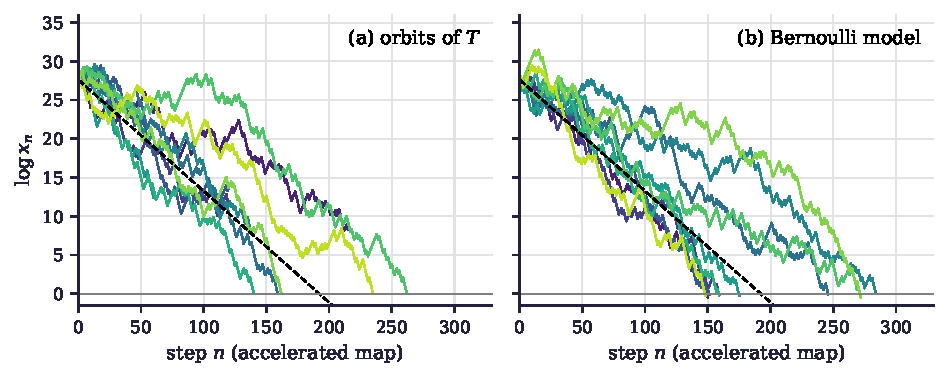
\includegraphics[width=\textwidth]{figures/ch3_paths.pdf}
\caption{Left: $\log x_n$ along ten orbits of the accelerated map started at
odd integers near $10^{12}$. Right: ten paths of the Bernoulli model from the
same height. The dashed line is the mean path $\log x_0+n\ds$.}
\label{fig:ch3:paths}
\end{figure}

\begin{remark}[The constant $14.58$ elsewhere in the book]\label{rem:ch3:c1458}
The number $C=(\log3/\log\frac43)^2$ appears again in \cref{chap:smm}, as the
condition number\index{condition number} at which the Switching MM\index{Switching MM} momentum\index{momentum} coefficient
$\beta=\log(3/2)/\log2$ is the optimal Nesterov\index{Nesterov acceleration} coefficient. This is the same
algebra and not a second piece of evidence: with $\beta=\lt-1$ one has
$(1+\beta)/(1-\beta)=\log3/\log\frac43$ exactly.
\end{remark}

\paragraph{The tail of the stopping time.} The first time $\nu$ at which a
model path falls below its starting height, the model counterpart of the
stopping time $\sigma(n)$ of the map, satisfies
$\Prob(\nu>n)\le\Prob(S_n\ge0)\le\E[e^{\theta S_n}]=M(\theta)^n$ for every
$\theta>0$, by Markov's inequality (this $\theta$ is not the $\theta$ of \cref{thm:density}). The minimum of $M$ is attained at
$\theta=\log(\log2/\log\frac32)/\log3\approx0.4881$, where
$M(\theta)\approx0.9659$. Thus $\Prob(\nu>n)\le0.9659^n$. This is the bound
$e^{-Dk}$ of \cref{thm:density}, obtained there by a Chernoff\index{large deviations} argument for the
binomial count of odd steps; the two computations are the same optimization in
different coordinates, since \cref{prop:ch3:exact} identifies the binomial
count with the number of factors $\tfrac32$ in the model.

\section{The central limit theorem for total stopping times}\label{sec:ch3:clt}

Wald's identity\index{Wald identity} gives the mean of $\tau$; the central limit theorem\index{central limit theorem} for first
passage times gives its fluctuations. For a random walk whose increments have
mean $\mu<0$ and variance $\sigma^2$, the first passage time
$\tau_u=\inf\{n:S_n\le-u\}$ satisfies, as $u\to\infty$,
\begin{equation}\label{eq:ch3:clt}
  \frac{\tau_u-u/|\mu|}{\sqrt{\sigma^2u/|\mu|^3}}\;\Longrightarrow\;N(0,1).
\end{equation}
This is a classical consequence of Anscombe's theorem and the central limit
theorem for the walk; see Gut~\cite{gut1988} for a complete treatment. A limit
in distribution does not by itself give the moments: that $\E[\tau_u]\sim u/|\mu|$
and $\Var(\tau_u)\sim\sigma^2u/|\mu|^3$ is the classical first passage
asymptotics of Heyde\index{Heyde, C. C.}~\cite{heyde1967} and
Siegmund\index{Siegmund, D.}~\cite{siegmund1969} (see
\cite[Theorem~III.9.1]{gut1988}). The
heuristic is quickly told. At time $t=u/|\mu|$ the walk sits at $-u$ plus a
fluctuation of order $\sigma\sqrt t$, and closing that gap at speed $|\mu|$
takes an extra time of order $\sigma\sqrt t/|\mu|$, whose variance is
$\sigma^2t/\mu^2=\sigma^2u/|\mu|^3$.

With $u=\log x_0$, $\mu=\ds$ and $\sigma^2=\frac14(\log3)^2$, the passage time
$\tau_u$ is the time $\tau$ of \cref{prop:lyapunov}, and the model
predicts that it is approximately normal with mean
$\gamma_0\log x_0$ and variance $\sigma^2\log x_0/|\ds|^3\approx101.4\log x_0$.
For this model the normal limit with exactly these constants was proved by
Borovkov\index{Borovkov, K. A.} and Pfeifer\index{Pfeifer, D.}~\cite[Theorem~5]{borovkov2001}.
Both constants are fixed by the drift and the variance of a single step, so the
prediction has no free parameter.
The ratio of the variance to the mean is $C=\sigma^2/(\ds)^2\approx14.58$,
which explains the name index of dispersion in \cref{prop:lyapunov}.
The counterpart of $\tau$ for the map is the total stopping time\index{stopping time}
$\sigma_\infty(n)$ of $T$, the number of steps of $T$ that take $n$ to $1$ (in
\cref{chap:intro} the same symbol counts steps of $T_0$). It is a deterministic
integer, and what can be compared with the law of $\tau$ is its spread over
many starting values $n$.

\begin{table}[t]
\centering
\caption{Total stopping time $\sigma_\infty(n)$ of the accelerated map for
$4000$ starting values $n$ drawn independently and uniformly from each range,
against the leading terms of the Bernoulli model, $\gamma_0\log n$ for the mean (a lower bound for the model mean, by \eqref{eq:ch3:waldbound}) and $101.4\log n$ for the variance, averaged over the sample.}
\label{tab:ch3:clt}
\small
\begin{tabular}{@{}lrrrrr@{}}
\toprule
Range of $n$ & Mean & $\gamma_0\log n$ & Variance & $101.4\log n$ & Ratio\\
\midrule
$[10^3,2\cdot10^3)$ & $49.66$ & $50.73$ & $685.3$ & $739.8$ & $0.926$\\
$[10^4,2\cdot10^4)$ & $65.36$ & $66.69$ & $871.2$ & $972.6$ & $0.896$\\
$[10^5,2\cdot10^5)$ & $81.18$ & $82.76$ & $1101.8$ & $1206.9$ & $0.913$\\
$[10^6,2\cdot10^6)$ & $96.90$ & $98.74$ & $1292.5$ & $1440.0$ & $0.898$\\
$[10^7,2\cdot10^7)$ & $114.33$ & $114.71$ & $1538.3$ & $1672.9$ & $0.920$\\
\bottomrule
\end{tabular}
\end{table}

\Cref{tab:ch3:clt} tests both predictions on samples of $4000$ starting values
drawn independently and uniformly, of either parity, from five ranges
(consecutive integers would not give independent samples, since their orbits
share their tails).
The means fall short of $\gamma_0\log n$ by $0.4$ to $1.8$ steps, whereas by \eqref{eq:ch3:waldbound} the model mean lies above $\gamma_0\log n$, and the overshoot of the barrier puts it $2.07$ steps higher in every range (script \texttt{ch3\_model\_means.py}).
So the real orbits are shorter than model paths from the same height, by $2.5$ to $3.9$ steps in these samples, whose means have standard errors of $0.4$ to $0.6$, and by $3.5$ steps in the exact census at $k=29$ of \cref{sec:ch3:missing}; the overshoot does not explain the shortfall but adds to it.
It is a boundary effect at the end of the orbit: a
real orbit stops on hitting $1$ exactly, with no overshoot, and small integers such as the powers
of two descend to $1$ faster than a random walk from the same height would.
(The $+1$ acts in the opposite direction, lengthening orbits by about one step on average, almost all of it in the final descent; see \cref{sec:ch3:missing}.)
The variances are about $0.9$ times the leading term $101.4\log n$ in every range; the exact variance of the model exceeds its leading term by $2$ to $4$ percent at these sizes, so the variances of the map are $0.87$ to $0.90$ times those of the model, with no clear trend at this sample size; \cref{sec:ch3:missing} locates the deficit exactly.
\Cref{fig:ch3:stopping} shows the regression of total stopping time on $\log n$ and
the pooled standardized residuals
$(\sigma_\infty(n)-\gamma_0\log n)/\sqrt{101.4\log n}$, whose sample variance is $0.909$
and whose skewness is $0.57$; first passage times of a walk with drift\index{drift} are
right skewed at finite $u$, and the skew decays like $u^{-1/2}$.

\begin{figure}[t]
\centering
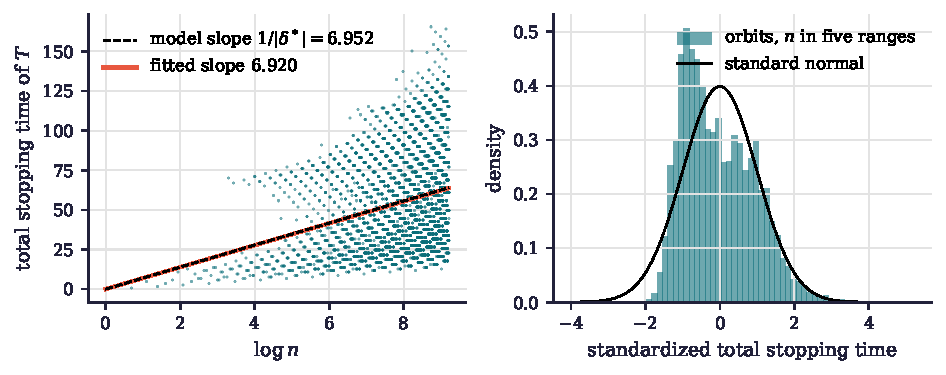
\includegraphics[width=\textwidth]{figures/ch3_stopping.pdf}
\caption{Left: total stopping time of $T$ against $\log n$ for $2\le n\le10^4$,
with the model slope $\gamma_0$ (dashed) and the fitted slope (solid).
Right: standardized total stopping times for $20000$ random $n$ from the five ranges
of \cref{tab:ch3:clt}, against the standard normal density.}
\label{fig:ch3:stopping}
\end{figure}

The conclusion is that the model gets the dispersion of total stopping times right
to about ten percent, erring slightly on the side of too much variability.
There is no excess dispersion to explain. This matters because it is easy to
construct a wrong explanation for a discrepancy that is not there; we return to
this in \cref{rem:ch3:variance}.

\section{Where the missing variance lives}\label{sec:ch3:missing}

The ten percent deficit in \cref{tab:ch3:clt} is small, but it is systematic,
and a complete census
locates its source. For every $n<2^{30}$ we computed the total stopping time\index{stopping time}
$\sigma_\infty(n)$ of $T$ and the number $a(n)$ of odd steps on the way to $1$ (script
\texttt{ch3\_o4\_decomp.py}, which takes about two minutes), and analysed each
dyadic block $[2^k,2^{k+1})$ exactly, not by sampling. The analysis rests on an
identity that holds orbit by orbit.

\begin{proposition}[Pathwise decomposition]\label{prop:ch3:pathwise}
For every $n\ge2$ whose orbit reaches $1$ (as every $n<2^{30}$ of the census does), with $u=\log n$ and $|\ds|=\log(2/\sqrt3)$,
\begin{gather*}
  |\ds|\,\sigma_\infty(n)=u+R(n)+Z(n),\\
  R=\sigma_\infty\log2-a\log3-u,\qquad Z=\tfrac12\log3\,(2a-\sigma_\infty).
\end{gather*}
Here $Z$ is the centred parity sum, a sum of $\sigma_\infty$ terms $\pm\frac12\log3$, and
$R=\sum_{\text{odd steps}}\log(1+1/(3x_i))\ge0$ is the total contribution of the
$+1$ terms. Splitting $Z=Z_{\mathrm h}+Z_{\mathrm t}$ into the sums over the first
$k$ steps and over the rest, for $n$ uniform in $[2^k,2^{k+1})$ the head
$Z_{\mathrm h}$ is exactly a sum of $k$ independent fair signs, so that
$\Var Z_{\mathrm h}=\sigma^2k$ with $\sigma^2=\frac14(\log3)^2$.
\end{proposition}

\begin{proof}
The identity is algebra: $u+R+Z=\sigma_\infty\log2-a\log3+a\log3-\frac12\sigma_\infty\log3=
\sigma_\infty(\log2-\frac12\log3)$. Taking logarithms along the orbit,
$0=\log1=u+a\log\frac32-(\sigma_\infty-a)\log2+\sum_{\text{odd}}\log(1+1/(3x_i))$, which
identifies $R$ with the sum of the $+1$ corrections. For the head, the block
$[2^k,2^{k+1})$ contains each residue class modulo $2^k$ exactly once, and by
\cref{thm:terras} the first $k$ parities are a bijective function of the class;
so they are uniformly distributed over $\{0,1\}^k$, that is, independent fair
bits.
\end{proof}

In the Bernoulli model\index{Bernoulli model} $Z$ would be a martingale\index{martingale} stopped at $\tau$, with
$\E Z^2=\sigma^2\E\tau$ by Wald's second identity\index{Wald identity}, and $R$ would be a bounded
overshoot; the model variance $\sigma^2\log n/|\ds|^3$ is the leading term of
$\Var(Z)/|\ds|^2$. \Cref{tab:ch3:missing} compares each piece with its model
value.

\begin{table}[ht]
\centering\small
\caption{Exact census of the dyadic blocks $[2^k,2^{k+1})$: mean and variance of
$\sigma_\infty$, the leading term $\sigma^2\E\log n/|\ds|^3$ of the model variance, the head ratio $\Var
Z_{\mathrm h}/(\sigma^2k)$, the tail ratio $\Var Z_{\mathrm t}/(\sigma^2\E(\sigma_\infty-k))$,
and the additive deficit $D_{\mathrm v}=\sigma^2\E(\sigma_\infty-k)-\Var Z_{\mathrm t}$.}
\label{tab:ch3:missing}
\setlength{\tabcolsep}{4pt}
\begin{tabular}{@{}rrrrcccr@{}}
\toprule
$k$ & $\E\sigma_\infty$ & $\Var\sigma_\infty$ & model & ratio & head & tail & $D_{\mathrm v}$ \\
\midrule
$10$ & $50.1$ & $709$ & $742$ & $0.956$ & $1.0000$ & $0.939$ & $0.74$ \\
$15$ & $73.6$ & $977$ & $1093$ & $0.894$ & $1.0000$ & $0.909$ & $1.61$ \\
$20$ & $97.7$ & $1308$ & $1445$ & $0.905$ & $1.0000$ & $0.902$ & $2.30$ \\
$25$ & $121.7$ & $1656$ & $1796$ & $0.922$ & $1.0000$ & $0.914$ & $2.51$ \\
$29$ & $141.0$ & $1938$ & $2077$ & $0.933$ & $1.0000$ & $0.924$ & $2.56$ \\
\bottomrule
\end{tabular}
\end{table}

Three conclusions follow. First, the head is exact, as the proposition
requires, and the plus one term $R$ contributes almost nothing to the variance: its
variance is $0.003$ in every block from $k=10$ on, and its covariance with $Z$
is about $0.05$. (Its mean, about $0.15$ in every block and so contributed almost entirely by the final descent, lengthens orbits by about one step.) The whole deficit lives in the tail parity sum, the part of the
orbit beyond the Terras\index{Terras, R.} horizon.

Second, the deficit is \emph{additive}, not multiplicative. The quantity $D_{\mathrm v}$ grows
from $0.74$ at $k=10$ and levels off near $2.6$ (in units of $\log^2$, about
$124$ squared steps of $T$), while the model variance grows linearly in $k$. So
the ratio of observed to model variance first falls, to a minimum near $0.89$
around $k=15$, and then rises again, to $0.933$ at $k=29$. If $D_{\mathrm v}$ stays bounded,
as the census suggests, the ratio tends to $1$ like $1-c/\log n$, and the model is
asymptotically exact to second order. At $n\approx10^{12}$ a saturated deficit
of $2.6$ would give a ratio of about $0.95$.

Third, the deficit sits at the end of the orbit. Splitting each orbit of a random
sample at the first time it falls below $Y=2^{14}$ (script
\texttt{ch3\_o4\_end.py}), the final segment from below $2^{14}$ down to $1$
contributes a deficit of $1.94$ to $1.98$ for $k=20$, $24$ and $28$, independent
of $k$, and is uncorrelated with what came before; the middle segment, from the
Terras horizon down to $2^{14}$, contributes $0.40$, $0.62$ and $0.64$, with its variance ratio
rising towards $1$ as $k$ grows ($0.914$, $0.930$, $0.952$). The final segment is
a finite deterministic system: every orbit enters $[1,2^{14})$ and then follows
one of finitely many fixed paths to $1$. Those paths are shorter and less
variable than a random walk descending from the same heights, because the
small integers are funnelled into a few common tails, through $20$, $10$, $5$ and the
powers of two. The model treats the last sixty or so steps as fresh coin flips,
and they are not.

So the census indicates that the deficit is a bounded boundary
effect at the bottom of the orbit, plus a smaller contribution from the passage
to the bottom, and that the Bernoulli model is asymptotically right about the
variance; a proof that the deficit stays bounded is the first part of open
problem O4 of \cref{chap:open}. The third cumulant is less well explained: the observed skewness of
$\sigma_\infty$ is $0.62$ at $k=20$ and $0.67$ at $k=29$, while the inverse Gaussian law
of a drifted Brownian first passage, with the model's drift\index{drift} and variance,
predicts $3\sigma/\sqrt{|\ds|\,\E\log n}$, which is $1.15$ and $0.96$. The real
total stopping times are less skewed than the model's passage times, and we leave the explanation
open.

\section{Excursions: the Ville and Lundberg bound}\label{sec:ch3:ville}

How high can an orbit climb before it descends? The orbit of $27$ under $T_0$ climbs to
$9232$, a factor of about $342$ (under $T$ its peak is $4616$), and such excursions are the most visible
feature of the problem. In the model the answer is controlled exactly by the
martingale\index{martingale} property, through a maximal inequality that goes back to
Ville\index{Ville inequality}\index{Ville, J.}~\cite{ville1939}.

\begin{proposition}[Ville bound]\label{prop:ch3:ville}
In the Bernoulli model\index{Bernoulli model} for $T$, for every $x_0>0$ and $K\geq1$,
\[
  \Prob\Bigl(\sup_{n\geq0}x_n\geq Kx_0\Bigr)\;\le\;\frac1K .
\]
Equivalently, in terms of the log walk, $\Prob(\sup_nS_n\geq u)\le e^{-u}$ for
every $u\geq0$. The same bound holds in the stride model for $S$, and in the
renewal\index{renewal theory} model for $T_0$ when $B_0=0$; when $B_0=1$ the bound becomes $3/K$.
\end{proposition}

\begin{proof}
Let $c=Kx_0$ and $\eta=\inf\{n:x_n\geq c\}$. The stopped process
$x_{n\wedge\eta}$ is a nonnegative martingale, so for each $n$
\[
  x_0=\E[x_{n\wedge\eta}]\geq\E[x_\eta;\eta\le n]\geq c\,\Prob(\eta\le n).
\]
Letting $n\to\infty$ gives $\Prob(\eta<\infty)\le x_0/c=1/K$. For the stride
model apply the same argument to the martingale $X_j$; the supremum over
strides is the supremum over odd values, which is the relevant one. For the
renewal model apply it to $M_n=3^{B_n}x_n\geq x_n$, whose initial value is
$3^{B_0}x_0$.
\end{proof}

The proposition is the Lundberg inequality of risk theory in the special case
$\theta^*=1$. For a general walk with negative drift\index{drift} the bound reads
$\Prob(\sup_nS_n\geq u)\le e^{-\theta^*u}$, and the Cram\'er and Lundberg
approximation sharpens it to $\Prob(\sup_nS_n\geq u)\sim C_{\mathrm L}e^{-\theta^*u}$ for a
constant $C_{\mathrm L}<1$ that depends on the overshoot over the level~\cite{asmussen2010}.
For the Collatz model this says that $K\cdot\Prob(\sup x_n\geq Kx_0)$ should
settle to a constant a little below one.

\Cref{fig:ch3:ville} tests the bound. For each $n$ with $2\le n\le10^6$ we
computed the maximum of the orbit of $n$ under $T$ and recorded the fraction of
$n$ whose maximum is at least $Kn$, for $K=2,4,\ldots,4096$. The product $K$
times this fraction lies between $0.76$ and $0.85$ for $K\le1024$, comfortably
below the bound. A simulation of $10^6$ paths of the Bernoulli model gives
values between $0.82$ and $0.85$ over the same range, an estimate of the
Cram\'er and Lundberg constant. The orbits sit a little below the model, in
line with the slightly smaller dispersion found in \cref{sec:ch3:clt}. The drop
at $K=2048$ and $K=4096$ is an edge effect: at these factors only a few hundred
of the million starting values qualify, and the integers below $10^6$ are too
small for the orbit to have room to make such excursions in the proportion the
model predicts.

\begin{figure}[t]
\centering
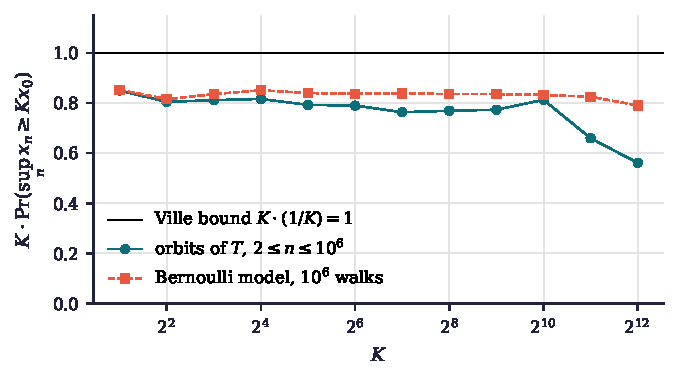
\includegraphics[width=\textwidth]{figures/ch3_ville.pdf}
\caption{The quantity $K\cdot\Prob(\sup_nx_n\geq Kx_0)$ for orbits of $T$
with $2\le n\le10^6$ (circles) and for $10^6$ paths of the Bernoulli model
(squares). For the model, Ville's inequality (\cref{prop:ch3:ville}) says that it never exceeds $1$.}
\label{fig:ch3:ville}
\end{figure}

\paragraph{The exponent $2$.} The Ville bound explains a prediction of
Lagarias\index{Lagarias, J. C.} and Weiss\index{Weiss, A.}~\cite{lagarias1992} about the maximal excursion
$t(n)=\max_kT^{(k)}(n)$. Treat the orbits of different $n$ as independent
model paths. Taking $K=n^{1+\varepsilon}$ gives
$\Prob(t(n)\geq n^{2+\varepsilon})\le n^{-1-\varepsilon}$, which is summable,
so by the Borel and Cantelli lemma only finitely many $n$ would have
$t(n)\geq n^{2+\varepsilon}$. In the other direction the Cram\'er and Lundberg
asymptotics give $\Prob(t(n)\geq n^{2-\varepsilon})\approx C_{\mathrm L}n^{-1+\varepsilon}$,
which is not summable, and independence would give infinitely many such $n$.
The heuristic conclusion is $\limsup_n\log t(n)/\log n=2$. Over
$1000<n\le10^6$ the largest value of $\log t(n)/\log n$ for the accelerated map\index{accelerated map}
is $1.9095$, attained at $n=159487$. The heuristic is of course only as good
as the independence assumption, which is false for neighbouring integers whose
orbits merge, and there is no proof that $t(n)\le n^{C}$ for any constant $C$.

\section{Parity autocorrelations}\label{sec:ch3:autocorr}

Under the accelerated map\index{accelerated map} the model parities are independent. Under the
standard map\index{standard map} they are not, and their dependence can be computed exactly.

\begin{proposition}[Parity autocorrelation function]\label{thm:autocorr}
In the renewal\index{renewal theory} model for $T_0$, started from its stationary law, the model
parity chain $(B_n)$ is stationary with
\[
  \Prob(B_n=1)=\frac{1}{1+\E[K]}=\frac13,\qquad\Var(B_n)=\frac29,
\]
and its autocorrelation\index{autocorrelation} function is
\begin{equation}\label{eq:ch3:rhoh}
  \rho(h)=\mathrm{Corr}(B_n,B_{n+h})=\Bigl(-\frac12\Bigr)^{h},\qquad h\geq0 .
\end{equation}
\end{proposition}

\begin{proof}
We give the renewal proof, which explains where the formula comes from; a
second proof is in \cref{rem:ch3:markov}. By
\cref{prop:ch3:standard}(v), the gaps between successive ones of $(B_n)$ are
independent copies of $G=1+K$, with
\[
  \Prob(G=m)=\Prob(K=m-1)=2^{-(m-1)},\qquad m\geq2 .
\]
Hence $\E[G]=1+\E[K]=3$, and by the renewal theorem the stationary probability
of a one is $1/\E[G]=\frac13$, so $\Var(B_n)=\frac13\cdot\frac23=\frac29$. The
generating function of the gap law is
\[
  F(z)=\sum_{m\geq2}2^{-(m-1)}z^m=\frac{z^2}{2-z},\qquad|z|<2 .
\]
Let $u(h)=\Prob(B_{n+h}=1\mid B_n=1)$ be the renewal sequence, with $u(0)=1$.
Decomposing according to the time of the first renewal after time $n$ gives the
renewal equation $u(h)=\sum_{m=1}^{h}\Prob(G=m)u(h-m)$ for $h\geq1$, which in
generating functions reads $U(z)=1+F(z)U(z)$, where
$U(z)=\sum_{h\geq0}u(h)z^h$. Therefore
\[
  U(z)=\frac{1}{1-F(z)}=\frac{2-z}{2-z-z^2}=\frac{2-z}{(1-z)(2+z)} .
\]
Partial fractions give
\[
  U(z)=\frac{1/3}{1-z}+\frac{4/3}{2+z}
      =\frac{1/3}{1-z}+\frac{2/3}{1+z/2},
\]
and expanding both terms as geometric series,
\begin{equation}\label{eq:ch3:renewal}
  u(h)=\frac13+\frac23\Bigl(-\frac12\Bigr)^{h},\qquad h\geq0 .
\end{equation}
The first values are $u(0)=1$, $u(1)=0$, $u(2)=\frac12$, $u(3)=\frac14$,
$u(4)=\frac38$. Finally, with $p=\frac13$,
\begin{align*}
  \rho(h)&=\frac{\Prob(B_n=1,B_{n+h}=1)-p^2}{p(1-p)}=\frac{p\,u(h)-p^2}{p(1-p)}\\
  &=\frac{u(h)-p}{1-p}=\frac32\Bigl(u(h)-\frac13\Bigr)=\Bigl(-\frac12\Bigr)^{h}. \qedhere
\end{align*}
\end{proof}

The first three values of the renewal sequence carry the arithmetic of a single stride.
$u(1)=0$ is \cref{prop:nocons}: there are never two consecutive odd steps.
$u(2)=\tfrac12$ and $u(3)=\tfrac14$ are the probabilities that the halving exponent equals $1$ and $2$, that is $\Prob(x\equiv3\pmod4)$ and $\Prob(x\equiv1\pmod8)$ for odd $x$ (\cref{prop:geom}).
From $h=4$ on the values involve the joint law of successive halving exponents, beginning with $u(4)=\Prob(K=3)+\Prob(K=1)^2=\tfrac38$; that law is exact for random residues over the range of \cref{prop:ch3:exact}, and beyond it the independence of successive exponents is an assumption of the model.

\begin{remark}[A second proof]\label{rem:ch3:markov}
Since $(B_n)$ is a Markov chain with transition matrix $P$, the conditional
law of $B_{n+h}$ given $B_n$ is given by $P^h$. Writing $P=\Pi+(-\tfrac12)E$ with
$\Pi$ the rank one projection onto the stationary vector and $E$ the
complementary spectral projection, $P^h=\Pi+(-\tfrac12)^hE$, and the
autocorrelation of any function of a reversible two state chain decays like
the $h$th power of the second eigenvalue. The renewal proof has the advantage
of exhibiting the generating function $U(z)$, which is what one needs for
the variance computation below.
\end{remark}

\begin{corollary}[Long run variance of the log path]\label{cor:longrun}
In the renewal model for $T_0$, the autocorrelation factor is
\[
  \mathcal{A}:=1+2\sum_{h\geq1}\rho(h)=1+2\cdot\frac{-1/2}{1+1/2}=\frac13 ,
\]
and the variance of the log path satisfies
\[
  \frac{\Var(\log x_n)}{n}\;\longrightarrow\;\mathcal{A}\cdot\frac29(\log6)^2
  =\frac{2}{27}(\log6)^2\approx0.2378 .
\]
\end{corollary}

\begin{proof}
The log increment at step $n$ is $B_n\log3-(1-B_n)\log2=B_n\log6-\log2$, a
linear function of $B_n$ with slope $\log6$. For a stationary sequence with
summable autocovariances we have
$\Var(\sum_{i<n}B_i)/n\to\Var(B)\,\mathcal{A}$.
The same limit holds from any initial state: the parities form a two state Markov chain whose second eigenvalue is $-\tfrac12$, so the law of $B_i$ approaches the stationary law geometrically fast, which changes $\Var(\sum_{i<n}B_i)$ by $O(1)$.
Here $\Var(B)=\frac29$ and $\sum_{h\geq1}(-\tfrac12)^h=-\tfrac13$, so
$\mathcal{A}=\frac13$ and the limit is $\frac13\cdot\frac29(\log6)^2$. As a
check, the variance asymptotic of renewal theory~\cite[Theorem~III.9.1]{gut1988} says that the
number $a_n$ of renewals before time $n$ has
$\Var(a_n)/n\to\Var(G)/\E[G]^3=2/27$, since $\Var(G)=\Var(K)=2$ and
$\E[G]=3$; and $\log x_n=\log x_0+a_n\log6-n\log2$. The two routes agree.
\end{proof}

\Cref{cor:longrun} has a consequence that runs against a natural intuition.

\begin{remark}[A tempting but false argument]\label{rem:ch3:variance}
One might argue as follows: ``the parities of $T_0$ are correlated, correlated
increments make a random walk more variable than an independent one, and so
the parity correlations should inflate the dispersion of total stopping times\index{stopping time} well
beyond what an independent model predicts.'' Each clause sounds reasonable, and
the conclusion is wrong in sign. The correlations are negative at odd lags and
alternate, $\rho(h)=(-\frac12)^h$, and their sum is $-\frac13$. The long run
variance factor is $\mathcal{A}=\frac13<1$, so the correlations \emph{reduce}
the variance of the log path by a factor of three relative to an independent
sequence with the same marginal law. Negative lag one correlation is exactly
what one expects from a forced halving after every tripling: an up step is
always cancelled in part by the next step. Two further facts close the
question. First, measured on the clock of $T$, where the model parities are
independent, the reduction disappears and what remains is the variance
$\sigma^2$ of \cref{prop:lyapunov}; the factor $\frac13$ and the deletion of
forced steps are two descriptions of the same thing. So $\mathcal{A}$ concerns
only the log path of $T_0$ counted in its own steps, and parity correlations
play no part in the dispersion law of \cref{sec:ch3:clt}, which is stated on
the clock of $T$. Second, as
\cref{tab:ch3:clt} shows, there is no excess dispersion of total stopping times to
explain: the observed variance is about $0.9$ of the model value. Any
mechanism that predicts an inflation of the variance by a large factor, from
parity correlations or from anything else, is contradicted by the data.
\end{remark}

\subsection{The empirical check}

\Cref{fig:ch3:acf} compares \eqref{eq:ch3:rhoh} with two empirical
autocorrelation\index{autocorrelation} functions for the parity sequence $b_j$ of $T_0$, both
estimated with the mean and variance pooled over all recorded steps: if $\hat p$
is the fraction of odd steps, the estimate at lag $h$ is
$(\overline{b_jb_{j+h}}-\hat p^{\,2})/(\hat p(1-\hat p))$, where the bar is the
average over all recorded pairs of steps $h$ apart. The first is a scan
over small starting values: orbits started at $27$ and then restarted at a
random odd number below $10^4$ each time they reach $1$, for a total of
$4\times10^5$ steps. These orbits are not truncated but followed all the way to
$1$. The fraction of odd steps is $0.3351$ and the first six lags are
\[
  -0.5040,\quad+0.2482,\quad-0.1530,\quad+0.0822,\quad-0.0032,\quad-0.0139,
\]
against the predicted values $(-\tfrac12)^h$, that is $-0.5$, $+0.25$, $-0.125$,
$+0.0625$, $-0.0313$ and $+0.0156$.
The first two lags agree (at lag one this is forced: no two odd steps are consecutive, so the estimate is $-\hat p/(1-\hat p)$ whatever the orbits).
From lag three on the agreement is visibly worse, and lag six even has the wrong sign.
Lag three still reflects a single stride: the halving exponent $2$, which has probability $u(3)=\tfrac14$ in the model, occurs in only $23.3$ percent of the strides of the scan. We regard
this as a genuine feature of short orbits and not as sampling noise. Small
starting values have few bits, so most of each orbit lies outside the range of
\cref{prop:ch3:exact}, and the scan includes the final descent of every orbit
through the powers of two and the cycle $4\to2\to1$, whose parity pattern is
far from stationary.

The second check uses large starting values and truncated orbits. For $4000$
random integers $n$ between $2^{200}$ and $2^{208}$, of either parity and with
$n\bmod2^{200}$ uniformly distributed, we recorded the parities of steps $50$ to
$299$ of $T_0$, far above the trivial cycle. By \cref{prop:ch3:exact} all but
about one percent of these steps lie inside the range in
which the parities of $T$ are exactly independent and fair, so apart from that
one percent and from sampling error the model is a theorem here. The fraction of odd steps is $0.3330$, and
the autocorrelations are $-0.4993$, $+0.2497$, $-0.1252$, $+0.0629$,
$-0.0320$, $+0.0155$ for $h=1,\ldots,6$, in agreement with $(-\tfrac12)^h$ to
the precision of the sample. The renewal\index{renewal theory}
formula is exact for an ensemble of starting values over the initial segment
of their orbits; along the late part of short orbits it is a prediction, and
the prediction is visibly imperfect from lag three on.

\begin{figure}[t]
\centering
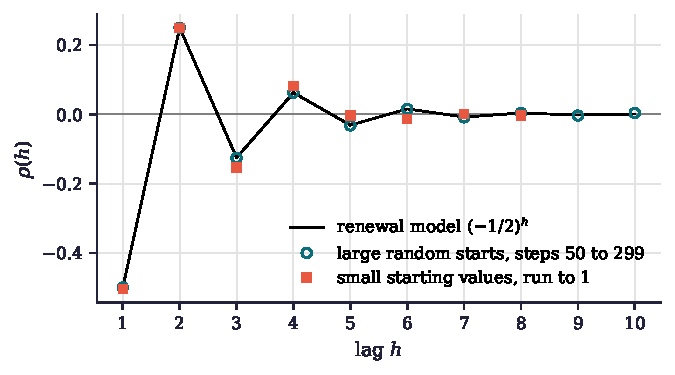
\includegraphics[width=\textwidth]{figures/ch3_acf.pdf}
\caption{Autocorrelation of the parity sequence of the standard map, estimated
with the pooled mean and variance. Solid
line: the renewal model $(-\tfrac12)^h$. Circles: $4000$ large random starting
values of either parity, steps $50$ to $299$. Squares: small odd starting values, orbits run to
$1$.}
\label{fig:ch3:acf}
\end{figure}

\section[Absorption and the failure of uniform integrability]{Absorption and the failure of\\ uniform integrability}\label{sec:ch3:absorb}

We now come to the two results that locate the obstruction precisely. The
first says that the model settles its own version of the conjecture. The
second says why the martingale\index{martingale} of \cref{thm:martingale} cannot be used to
settle it, even in the model.

\begin{proposition}[The model absorbs almost surely]\label{prop:absorb}
Let $\Delta_1,\Delta_2,\ldots$ be independent and identically distributed and
integrable with mean $\mu<0$, and put $\log x_n=\log x_0+\sum_{i\le n}\Delta_i$
with $x_0>1$. Let $\tau=\inf\{n:x_n\le1\}$. Then $\E[\tau]<\infty$; in
particular
\[
  \Prob\bigl(x_n>1\text{ for all }n\bigr)=0 .
\]
If moreover $\Delta_i\geq-L$ almost surely, then
$\E[\tau]<(\log x_0+L)/|\mu|$.
\end{proposition}

\begin{proof}
Suppose first that $\Delta_i\geq-L$. The process $N_n=\log x_n-n\mu$ is a
martingale, and optional stopping at the bounded time $n\wedge\tau$ gives
\[
  \E[\log x_{n\wedge\tau}]=\log x_0+\mu\,\E[n\wedge\tau] .
\]
Before time $\tau$ the value $\log x$ is positive, and at time $\tau$ it is at
least $\log x_{\tau-1}-L>-L$. Hence $\log x_{n\wedge\tau}>-L$, and
$|\mu|\,\E[n\wedge\tau]<\log x_0+L$. Monotone convergence as $n\to\infty$ gives
$|\mu|\,\E[\tau]\le\log x_0+L$.
So $\tau$ is integrable, Wald's identity\index{Wald identity} $\E[\log x_\tau]=\log x_0+\mu\,\E[\tau]$ holds, and since $\log x_\tau>-L$ almost surely the bound is strict.

In general, put $\Delta_i'=\max(\Delta_i,-L)$. As $L\to\infty$,
$\E[\Delta_i']$ decreases to $\mu$ by monotone convergence, so we may fix $L$
with $\mu'=\E[\Delta_i']<0$. The walk built from the $\Delta_i'$ lies above the
original walk, so its passage time $\tau'$ below $0$ satisfies
$\tau\le\tau'$, and by the first part $\E[\tau']<(\log x_0+L)/|\mu'|$. In
either case $\tau$ is integrable and therefore finite almost surely.
\end{proof}

For the Bernoulli model\index{Bernoulli model} $L=\log2$ and the bound is the upper half of
\eqref{eq:ch3:waldbound}. For the stride model the downward steps
$\log3-K\log2$ are unbounded, and the truncation in the second half of the
proof is needed.

The proposition is the strong law of large numbers in martingale dress, and the
dress is the point. Its only inputs are a negative mean and independence of the
increments from the past, which is what makes $N_n$ a martingale. For the
Collatz map the increments are deterministic functions of the current iterate,
there is no filtration with respect to which $\log x_n-n\ds$ is a martingale,
and \cref{prop:absorb} has no analogue. The Ces\`aro liminf conjecture of
\cref{chap:divergence} asks for a deterministic substitute for the part of this argument that excludes escape to infinity; it says nothing about cycles.

\begin{proposition}[Failure of uniform integrability]\label{prop:uimartingale}
In the Bernoulli model for $T$ with $x_0>1$, let $\tau=\inf\{n:x_n\le1\}$. Then
$\tau<\infty$ almost surely, the stopped process $(x_{n\wedge\tau})_{n\geq0}$ is
a nonnegative martingale converging almost surely to $x_\tau\le1$, and it is
not uniformly integrable\index{uniform integrability}. More precisely, for every $n$,
\[
  \E\bigl[x_n;\tau>n\bigr]\;\geq\;x_0-1,\qquad\text{while}\qquad
  \Prob(\tau>n)\to0 .
\]
\end{proposition}

\begin{proof}
Almost sure finiteness of $\tau$ is \cref{prop:absorb}. The stopped process of a
martingale is a martingale, so $\E[x_{n\wedge\tau}]=x_0$ for every $n$, and
\[
  x_0=\E[x_\tau;\tau\le n]+\E[x_n;\tau>n]\le\Prob(\tau\le n)+\E[x_n;\tau>n],
\]
which gives the first inequality. If the stopped process were uniformly
integrable, then $x_{n\wedge\tau}\to x_\tau$ in $L^1$, and
$x_0=\lim\E[x_{n\wedge\tau}]=\E[x_\tau]\le1$, a contradiction. Equivalently,
the expectations $\E[x_n;\tau>n]$ stay above $x_0-1>0$ on events whose
probabilities tend to zero, which is exactly the failure of uniform
integrability.
\end{proof}

The two propositions are consistent and together they locate the
obstruction. The martingale $(x_n)$ has constant mean $x_0$ while almost every
path is absorbed. The mass that keeps the mean up escapes along the rare paths
that have not yet been absorbed, and these paths carry, at every time $n$, an
expected value of at least $x_0-1$. Taking logarithms converts the martingale
into a supermartingale\index{supermartingale} with drift\index{drift}, which is why \cref{prop:absorb} works for
$\log x$ and cannot be run for $x$. The power functions $x^\theta$ with
$0<\theta<1$ sit in between: by \cref{thm:martingale}(iii) they are
supermartingales with geometric drift $M(\theta)<1$, and they are the model
counterpart of the power majorizer\index{majorization}s of \cref{chap:lyapunov}.

\begin{remark}[What a certificate would have to be]\label{rem:ch3:cert}
Suppose we tried to turn the model into a proof. In a probabilistic setting
one would look for a uniformly integrable martingale $Y_n$ that converges to the
indicator of absorption; then $Y_0=\Prob(\tau<\infty)$, and showing $Y_0=1$ is
the statement to be proved. Such a martingale always exists, namely
$Y_n=\Prob(\tau<\infty\mid\Filt_n)$, but writing it down requires knowing the
absorption probability, which is the thing to be proved; in the model it is
identically $1$ by \cref{prop:absorb}, so the certificate\index{certificate} is trivial and
uninformative. In the model the only martingales of the form $x_n^\theta$ are
those with $\theta=0$ and $\theta=1$, the roots of $M(\theta)=1$ in
\cref{thm:martingale}, and neither carries information about termination.

For the deterministic map the analogue of the conditional probability is the
function $h(x)=1$ if the orbit of $x$ reaches $1$ and $h(x)=0$ otherwise. It is
invariant, $h(T(x))=h(x)$, and the conjecture is the assertion $h\equiv1$. A
useful certificate would be a computable function $g\ge0$ that decreases along
orbits by a definite amount away from $1$, and \cref{chap:lyapunov} shows that
no such function that increases with $x$ exists, whatever fixed number of
strides is allowed for the decrease (\cref{thm:nolyapunov,cor:ch4:multistride}). What the model
offers instead is decrease in expectation, and expectation requires a measure.
The only measures for which the Collatz parities are provably independent are
the uniform measures on residue classes of \cref{prop:ch3:exact}, and they
control a single orbit for only as many steps as the residue class has bits. A
certificate along these lines would therefore have to show that the
information an orbit generates as it proceeds is, in a quantitative sense,
as good as fresh randomness. This is the content of the equidistribution\index{equidistribution}
questions of \cref{chap:divergence}, and it is where every known approach
stops.
\end{remark}

\section*{Notes}

\Cref{sec:ch3:heuristic} tells the history of the model; the survey of Kontorovich\index{Kontorovich, A. V.} and Lagarias~\cite{kontorovich2009} is the best general reference for stochastic models of the $3x+1$ and $5x+1$ problems. The presentation of
the martingale\index{martingale}
duality of \cref{thm:martingale}, the martingale $3^{B_n}x_n$ for the standard
map and the renewal computation of $\rho(h)=(-\tfrac12)^h$ and $\mathcal{A}=\frac13$
is ours, but all of these are elementary, and the closed form is the
autocorrelation of a two state Markov chain; the renewal\index{renewal theory} structure of the model parity
sequence is implicit in all treatments that use the Geometric law of the
halving exponent. The dispersion law of \cref{sec:ch3:clt} is the classical
first passage asymptotics of Heyde\index{Heyde, C. C.}~\cite{heyde1967} and
Siegmund\index{Siegmund, D.}~\cite{siegmund1969}; for this model
Borovkov\index{Borovkov, K. A.} and Pfeifer\index{Pfeifer, D.}~\cite[Theorem~5]{borovkov2001}
proved the normal limit with these constants.

For martingales, optional stopping and the convergence theorems we have used,
Williams\index{Williams, D.}~\cite{williams1991} is a concise and elegant source. Wald's identity\index{Wald identity}
is from Wald\index{Wald, A.}~\cite{wald1944}; the maximal inequality for nonnegative
supermartingales\index{supermartingale} appears in Ville\index{Ville inequality}\index{Ville, J.}'s thesis~\cite{ville1939}, which also
introduced the word martingale into probability. Renewal theory, the renewal
central limit theorem\index{central limit theorem} and the ladder variables behind the Cram\'er and Lundberg
approximation are in Feller\index{Feller, W.}~\cite{feller1971}; Gut\index{Gut, A.}~\cite{gut1988} treats
first passage times and Anscombe's theorem; Asmussen\index{Asmussen, S.} and
Albrecher\index{Albrecher, H.}~\cite{asmussen2010} is the standard reference for Lundberg
inequalities in risk theory, where the Wald root is called the adjustment
coefficient.

\begin{sloppypar}
All numerical results in this chapter were computed by the authors; the scripts
are \texttt{ch3\_stats.py}, \texttt{ch3\_stopping.py},
\texttt{ch3\_figures.py}, \texttt{ch3\_o4\_decomp.py}, \texttt{ch3\_o4\_census.py} and \texttt{ch3\_o4\_end.py} in the code appendix; the exact moments of the model passage time come from \texttt{ch3\_model\_means.py}, which uses \texttt{ch3\_o4\_model.py}.
\end{sloppypar}

\section*{Exercises}

\begin{exercise}\label{ex:ch3:fivex}
Repeat the computations of \cref{thm:martingale} for the $5x+1$ map, with
accelerated form $x\mapsto(5x+1)/2$ for odd $x$. Show that the log drift\index{drift} under
the fair coin model is $\frac12\log\frac54>0$, that the factors no longer have
mean one, and find the nonzero root of the moment generating function. What
does the sign of the root say about excursions?
\end{exercise}

\begin{exercise}\label{ex:ch3:wald}
In the stride model, let $\tau$ be the first stride at which $X_j\le1$. Use
Wald's identity\index{Wald identity} to show that $\E[\tau]=\log X_0/\log\frac43+O(1)$, and
reconcile this with the slope $\gamma_0$ of \cref{prop:lyapunov} by counting
steps of $T$ per stride.
\end{exercise}

\begin{exercise}\label{ex:ch3:renewal}
Let the halving exponent have a general law on $\{1,2,\ldots\}$ with
generating function $\phi(z)=\E[z^K]$. Show that the renewal\index{renewal theory} sequence of the
parity chain of $T_0$ has generating function $U(z)=1/(1-z\phi(z))$, and
verify \eqref{eq:ch3:renewal} for $\phi(z)=z/(2-z)$. For which laws of $K$ is
$\rho(2)>0$?
\end{exercise}

\begin{exercise}\label{ex:ch3:ville}
In the Bernoulli model\index{Bernoulli model}, let $\eta$ be the first time $x_n\geq Kx_0$ and
$\zeta$ the first time $x_n\le\varepsilon$, where $0<\varepsilon<x_0$. Apply
optional stopping to the bounded martingale\index{martingale} $x_{n\wedge\eta\wedge\zeta}$, using
the fact that a level is overshot by at most a factor $\frac32$, to show that
\[
  \frac{2}{3K}\;\le\;\Prob\Bigl(\sup_nx_n\geq Kx_0\Bigr)\;\le\;\frac1K .
\]
Thus the Ville\index{Ville inequality} bound is sharp up to a constant factor.
\end{exercise}

\begin{exercise}\label{ex:ch3:standardui}
In the renewal model for $T_0$, let $\tau$ be the first time $x_n\le1$, and suppose that $x_0>1$ and $3^{B_0}x_0>2$, that is, $x_0>2$ or $B_0=1$. Show
that the stopped martingale $M_{n\wedge\tau}$, with $M_n=3^{B_n}x_n$, is not
uniformly integrable\index{uniform integrability}, and that $\E[M_n;\tau>n]\geq3^{B_0}x_0-2$ for every $n$
while $\Prob(\tau>n)\to0$. (Hint: the step into $\tau$ is a halving, so $B_\tau$ is a fair coin independent of the past.) What happens when $B_0=0$ and $1<x_0\le2$?
\end{exercise}

\begin{exercise}\label{ex:ch3:simulate}
Write a program that estimates the Cram\'er and Lundberg constant
$C_{\mathrm L}=\lim_{K\to\infty}K\,\Prob(\sup_nx_n\geq Kx_0)$ for the Bernoulli model, and
compare your estimate with the values near $0.84$ reported in
\cref{sec:ch3:ville}.
\end{exercise}


\renewcommand{\partimagehook}{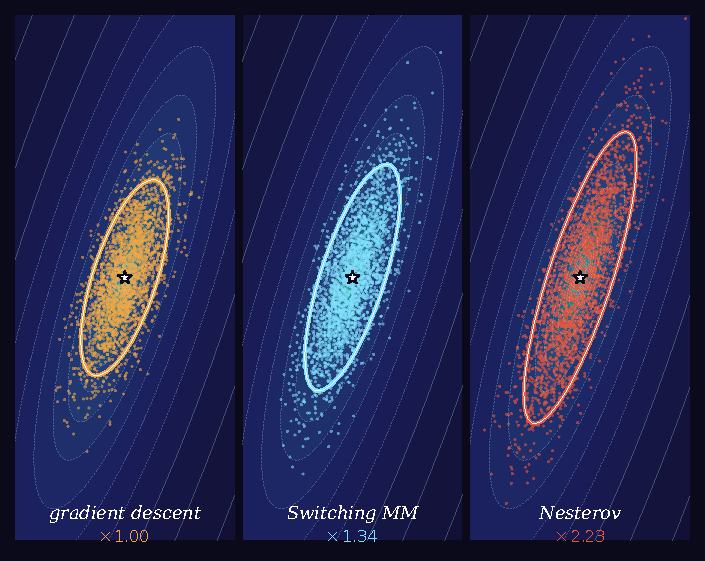
\includegraphics[width=1\textwidth]{figures/art_part2}\par\vspace{8pt}{\normalsize\upshape\itshape Stationary noise clouds of gradient descent, Switching MM and Nesterov ($\beta=\log_23-1$, step $1/L$) on a quadratic with condition number $20$ and noisy gradients; ellipses are two standard deviation contours of the exact stationary covariances, and the numbers give the stationary variance along the slow eigenvector relative to gradient descent ($1.36$ and $2.41$ in the limit of infinite condition number).\par}}
\part{The Optimization Reading}
\chapter{Lyapunov Functions and the Limits of Descent}\label{chap:lyapunov}

The heuristic that has accompanied the $3x+1$ problem since the work of
Terras\index{Terras, R.}~\cite{terras1976}, Crandall\index{Crandall, R. E.}~\cite{crandall1978} and Lagarias\index{Lagarias, J. C.} and Weiss\index{Weiss, A.}~\cite{lagarias1992} is, at
bottom, a statement about a potential function.  The quantity $\log x$ goes
down on average along a Collatz orbit, and a quantity that goes down on
average, and cannot go below zero, ought eventually to reach its floor.  In dynamical systems and optimization this is the language of Lyapunov functions\index{Lyapunov function}, and the purpose of this chapter is to take that language
seriously: to say precisely what a Lyapunov certificate\index{certificate} for the Collatz map
would be, to prove what can be proved about the natural candidates, and to
show, with complete proofs, why every candidate of the most natural kind must
fail.

The chapter has a positive half and a negative half.  The positive half is the
stride descent theorem, \cref{thm:stride}, which describes exactly when a
single Syracuse stride decreases $\log x$ and by how much, together with an
exact analysis of two stride compositions.  The negative half consists of
three obstructions.  No single stride Lyapunov function that is monotone in
the size of $x$ can certify descent (\cref{thm:nolyapunov}); no monotone certificate
built from any fixed number $J$ of strides can do so either, because ascending
strides can be chained to arbitrary length
(\cref{prop:ch4:chain,cor:ch4:multistride}); and the natural majorization\index{majorization}
minimization construction for $\log$ yields only a tangent line bound\index{MM algorithm},
which holds for any next iterate and whose surrogate drifts upward in the model
(\cref{prop:mmdescent,prop:mmfails}).  The last
obstruction has a clean explanation in terms of the martingale\index{martingale} duality of
\cref{chap:stochastic}, and it points to the family of power majorizers, which
repair the drift\index{drift} but not the pointwise failure.

Throughout, $S$ denotes the Syracuse map\index{Syracuse map} of \cref{def:maps},
$S(x)=(3x+1)/2^{k}$ with $k=\vt(3x+1)$, acting on odd positive integers, and
$T_0$ and $T$ denote the standard and accelerated map\index{accelerated map}s.

\section{Lyapunov functions for discrete dynamics}\label{sec:ch4:discrete}

Let $f:X\to X$ be a map on a set $X$ and let $A\subset X$ be a target set.
Lyapunov\index{Lyapunov, A. M.}'s idea, set out in his 1892 thesis on the stability of motion~\cite{lyapunov1992} and
carried into the discrete setting by LaSalle\index{LaSalle, J. P.} and others~\cite{lasalle1986}, is
to certify that orbits approach $A$ without computing them, by exhibiting a
scalar function that decreases along every orbit outside $A$.

\begin{definition}[Lyapunov certificate]\label{def:ch4:lyap}
A function $V:X\to\R$ is a \emph{Lyapunov function\index{Lyapunov function}} for $(f,A)$ if
$V(f(x))\le V(x)$ for every $x\notin A$.  It is a \emph{strict} Lyapunov
function if $V(f(x))<V(x)$ for every $x\notin A$, and a \emph{strong} (or
geometric) Lyapunov function if $V>0$ on $X\setminus A$ and there is a
constant $\rho<1$ with $V(f(x))\le\rho\,V(x)$ for every $x\notin A$.
\end{definition}

On a continuum, a strict Lyapunov function need not drive orbits into $A$;
the decrease can become arbitrarily small, and LaSalle's invariance principle
is the tool that identifies where such orbits accumulate~\cite{lasalle1986}.
The situation is simpler when $V$ takes values in the nonnegative integers, or decreases by at least a fixed amount, because a strictly decreasing sequence of nonnegative integers, or a sequence of reals bounded below that decreases by at least a fixed amount at each step, must stop.

\begin{proposition}[Discrete Lyapunov criterion]\label{prop:ch4:discrete}
Let $f:X\to X$ and $A\subset X$.  Suppose that either
\begin{enumerate}[label=(\roman*)]
\item $V$ takes values in $\N\cup\{0\}$ and $V(f(x))<V(x)$ for $x\notin A$; or
\item $V\ge0$ and there is $\varepsilon>0$ with $V(f(x))\le V(x)-\varepsilon$
  for $x\notin A$; or
\item $V\ge c>0$ on $X\setminus A$ and $V(f(x))\le\rho V(x)$ for $x\notin A$,
  with $\rho<1$.
\end{enumerate}
Then every orbit of $f$ enters $A$.  In case (ii) it does so within
$V(x)/\varepsilon$ steps, and in case (iii) within
$1+\log(V(x)/c)/\log(1/\rho)$ steps.
\end{proposition}

\begin{proof}
Suppose that the first $n\ge1$ points $x,f(x),\dots,f^{(n-1)}(x)$ of the orbit lie outside $A$. In case (i) $V$ takes the $n+1$ distinct values $V(x)>V(f(x))>\dots>V(f^{(n)}(x))$, all in $\{0,1,\dots,V(x)\}$, so $n\le V(x)$. In case (ii), $0\le V(f^{(n)}(x))\le V(x)-n\varepsilon$, so $n\le V(x)/\varepsilon$. In case (iii) the bound $V\ge c$ is known only outside $A$, so $c\le V(f^{(n-1)}(x))\le\rho^{n-1}V(x)$ and $n\le1+\log(V(x)/c)/\log(1/\rho)$. In each case $n$ is bounded, so the orbit enters $A$, and the number of steps it takes obeys the stated bound.
\end{proof}

The Collatz conjecture\index{Collatz conjecture} is equivalent to the existence of such a certificate\index{certificate},
and this is worth recording at the outset because it shows that existence is
not the issue.

\begin{remark}[Certificates exist if and only if the conjecture holds]
\label{rem:ch4:exists}
Let $X$ be the odd positive integers, $f=S$ and $A=\{1\}$.  If every Syracuse
orbit reaches $1$, let $\sigma_S(x)$ be the number of strides it takes.  Then
$V=\sigma_S$ satisfies case (i) of \cref{prop:ch4:discrete}, since
$\sigma_S(S(x))=\sigma_S(x)-1$, and $W=2^{\sigma_S}$ satisfies case (iii) with
$c=2$ and $\rho=\tfrac12$.  Conversely any certificate of the kind in
\cref{prop:ch4:discrete} proves that every orbit reaches $1$.  The difficulty
is therefore never whether a Lyapunov function exists but whether one can be
written down without knowing the answer.  The functions $\sigma_S$ and
$2^{\sigma_S}$ are wildly irregular in $x$; the candidates one can actually
analyse are smooth increasing functions of the size of $x$, and those are the ones this
chapter shows to be inadequate.
\end{remark}

\section[Stochastic Lyapunov functions and Foster's criterion]{Stochastic Lyapunov functions and\\ Foster's criterion}
\label{sec:ch4:foster}

The stochastic analogue of a Lyapunov function\index{Lyapunov function} replaces pointwise decrease by
decrease in conditional expectation.  The idea goes back to
Foster\index{Foster, F. G.}~\cite{foster1953}, who used it to decide positive recurrence of
countable Markov chains arising in queueing, and it is the organizing
principle of the monograph of Meyn\index{Meyn, S. P.} and Tweedie\index{Tweedie, R. L.}~\cite{meyn1993}, where it
appears in many forms under the name of drift\index{drift} conditions.

\begin{theorem}[Foster's criterion]\label{thm:ch4:foster}
Let $(X_n)$ be an irreducible Markov chain on a countable set $E$, let
$V:E\to[0,\infty)$, let $C\subset E$ be finite and $\varepsilon>0$.  Suppose
\begin{align*}
  \E\bigl[V(X_1)\mid X_0=x\bigr]&\le V(x)-\varepsilon &&(x\notin C),\\
  \E\bigl[V(X_1)\mid X_0=x\bigr]&<\infty &&(x\in C).
\end{align*}
Then the chain is positive recurrent.  Moreover, if $\tau_C$ is the hitting
time of $C$, then $\E_x[\tau_C]\le V(x)/\varepsilon$ for every $x\notin C$.
\end{theorem}

The positive recurrence statement is Foster's theorem~\cite{foster1953}; see
Meyn and Tweedie~\cite{meyn1993} for the general theory.  The hitting time
bound is elementary and we prove it, because it is exactly the stochastic
counterpart of case (ii) of \cref{prop:ch4:discrete}.

\begin{proof}[Proof of the hitting time bound]
Fix $x\notin C$ and put $M_n=V(X_{n\wedge\tau_C})+\varepsilon\,(n\wedge\tau_C)$.
On the event $\{\tau_C>n\}$ the drift condition gives
$\E[M_{n+1}\mid\Filt_n]\le V(X_n)-\varepsilon+\varepsilon(n+1)=M_n$, and on
$\{\tau_C\le n\}$ we have $M_{n+1}=M_n$.  So $(M_n)$ is a nonnegative
supermartingale\index{martingale}\index{supermartingale} and $\varepsilon\,\E_x[n\wedge\tau_C]\le\E_x[M_n]\le M_0=V(x)$.
Letting $n\to\infty$ and using monotone convergence gives
$\E_x[\tau_C]\le V(x)/\varepsilon$.
\end{proof}

The proof uses neither the countability of $E$, nor irreducibility, nor the finiteness of $C$, so it applies to the stride model of \cref{chap:stochastic}; but it does use $V\ge0$, through the nonnegativity of $(M_n)$, and this is where the obvious candidate fails. In the stride model the successive log increments $\Delta_j=\log 3-k_j\log 2$ are independent, with $k_j$ distributed as Geometric$(\tfrac12)$ (\cref{def:ch3:models}; \cref{prop:geom} is the arithmetic source of this law), so that $\E[\Delta_j]=\log 3-2\log2=\log(3/4)\approx-0.2877$. Write $x_j$ for the state after $j$ strides, and let $\tau$ be the first stride with $\log x_\tau\le0$. Taking $V=\log x$ and $C=\{\log x\le0\}$, the drift condition holds with $\varepsilon=|\log(3/4)|$, but at time $\tau$ the value of $V$ is $-O$, where $O=-\log x_\tau\ge0$ is the overshoot of the last stride below $0$, and $O>0$ with positive probability. So the argument fails, and the bound $\E_{x_0}[\tau]\le\log x_0/|\log(3/4)|$ that it would give is false: by the next proposition, $\log x_0/|\log(3/4)|$ is in fact a strict lower bound for $\E_{x_0}[\tau]$. The overshoot has to be paid for.

\begin{proposition}[Passage time of the stride model]\label{prop:ch4:passage}
In the stride model, let $x_0>1$, and let $\tau$ and $O$ be as above. Then $\log2\le\E[O]<2\log2$, and
\begin{equation}\label{eq:ch4:fosterbound}
  \frac{\log x_0+\log2}{|\log(3/4)|}\;\le\;\E_{x_0}[\tau]\;<\;\frac{\log x_0+2\log2}{|\log(3/4)|}.
\end{equation}
\end{proposition}

\begin{proof}
By \cref{prop:absorb}, $\tau$ is integrable, so Wald's identity\index{Wald identity}\index{Wald, A.} applies to the walk $\log x_j=\log x_0+\Delta_1+\dots+\Delta_j$ and gives $\E[\log x_\tau]=\log x_0+\log(3/4)\,\E_{x_0}[\tau]$, that is,
\[
  \E_{x_0}[\tau]=\frac{\log x_0+\E[O]}{|\log(3/4)|}.
\]
To bound $\E[O]$, suppose that $\log x_{j-1}=y>0$. Stride $j$ ends at or below $0$ exactly when $y+\log3-k_j\log2\le0$, that is, when $k_j\ge m$ with $m=\lceil(y+\log3)/\log2\rceil$, and then $O=(k_j-m)\log2+r$ with $r=m\log2-y-\log3\in[0,\log2)$. Since $k_j$ is independent of the first $j-1$ strides and the Geometric law has no memory, given $k_j\ge m$ the excess $k_j-m$ has the law of $k_j-1$, whose mean is $1$. So, given the first $j-1$ strides and $\tau=j$, the conditional mean of $O$ is $\log2+r$, which lies in $[\log2,2\log2)$. Averaging over $j$ and over the first $j-1$ strides, with total weight $\Prob(\tau<\infty)=1$, gives $\log2\le\E[O]<2\log2$, and \eqref{eq:ch4:fosterbound} follows.
\end{proof}

The model therefore needs about $3.476\log x_0$ strides, and the overshoot adds between $\log2/|\log(3/4)|\approx2.41$ and $4.82$ more. At $\log x_0=10$ the bounds are $37.17$ and $39.58$, against $34.76$ for the leading term alone, and an exact computation (script \texttt{ch4\_exact.py}) gives $\E[\tau]\approx38.19$ and $\E[O]\approx0.99$, in agreement with a simulation of $2\times10^5$ paths. Since a stride of the accelerated map\index{accelerated map} contains on average two steps, the leading term is the slope $\gamma_0=1/|\ds|\approx6.952$ of \cref{prop:lyapunov}, measured in strides instead of steps, and \eqref{eq:ch4:fosterbound} is the stride counterpart of \eqref{eq:ch3:waldbound}: in both, $\log x_0$ divided by the drift is a lower bound, and the overshoot accounts for the rest. In the model, then, $\log x$ becomes a Foster function once it is shifted to pay for the overshoot: the function equal to $\log x+2\log2$ off $C$ and to $0$ on $C$ is nonnegative and satisfies the drift condition with $\varepsilon=|\log(3/4)|$, and the hitting time bound gives the upper half of \eqref{eq:ch4:fosterbound} again, with $\le$ in place of $<$ (\cref{ex:ch4:passage}). The model's version of the conjecture follows, as \cref{prop:absorb} already showed by a martingale argument. The whole of this chapter is an investigation of what survives when the expectation is removed.

\section{The conjecture as a descent statement}\label{sec:ch4:descent}

The connection between the conjecture and the potential $V(x)=\log x$ is not
only heuristic.  Recall (\cref{def:ch2:stopping}) that the \emph{stopping time\index{stopping time}} $\sigma(n)$ of $n>1$ is the least $k\ge1$ with $T^{(k)}(n)<n$, or $\infty$ if there is none; it is finite exactly when some $T_0^{(j)}(n)<n$, because the iterates of $T$ are those of $T_0$ with the values $3m+1$ omitted, and such a value, being larger than the odd $m$ before it, is never the first iterate below $n$.
Terras\index{Terras, R.}~\cite{terras1976} and,
independently, Everett\index{Everett, C. J.}~\cite{everett1977} proved that
almost every $n$ has a finite stopping time (\cref{thm:density}); the
conjecture is exactly the statement that every $n$ does.

\begin{proposition}[The conjecture as eventual descent]\label{prop:ch4:eventual}
The following are equivalent.
\begin{enumerate}[label=(\roman*)]
\item Every positive integer eventually reaches $1$ under $T_0$.
\item For every integer $n>1$ there is $j\ge1$ with
  $\log T_0^{(j)}(n)<\log n$.
\end{enumerate}
\end{proposition}

\begin{proof}
If (i) holds and $n>1$, the orbit of $n$ reaches $1<n$, so (ii) holds.
Conversely, assume (ii) and suppose some integer fails to reach $1$; let $n$
be the least such.  Then $n>1$ (since $1\to4\to2\to1$), and by (ii) some
iterate $m=T_0^{(j)}(n)$ satisfies $m<n$.  By minimality $m$ reaches $1$,
hence so does $n$, a contradiction.
\end{proof}

So the conjecture asserts that $V=\log x$ is an \emph{eventual} Lyapunov
function: it need not decrease at every step, or at every stride, but from
every starting point it eventually drops below its initial value.  What one
would like is to replace ``eventually'' by a fixed horizon, or to replace
$\log x$ by a function that decreases at every step.  The rest of the chapter
shows that within the class of functions increasing in $x$ neither replacement is
possible.

\section{The stride descent theorem}\label{sec:ch4:stride}

The basic computation concerns one Syracuse stride.  For odd $x$ and
$k=\vt(3x+1)\ge1$,
\begin{equation}\label{eq:ch4:stride}
  \log S(x)-\log x=\log\Bigl(3+\frac1x\Bigr)-k\log2 .
\end{equation}
The first term lies in $(\log 3,\log(10/3)]$ for odd $x\ge3$; the second is a
positive integer multiple of $\log2$.  Since $\log2<\log3<\log4$, the sign
of the increment is decided entirely by whether $k=1$ or $k\ge2$.

\begin{theorem}[Stride descent]\label{thm:stride}
Let $x\ge3$ be odd and $k=\vt(3x+1)$.
\begin{enumerate}[label=(\roman*)]
\item $\log S(x)-\log x=\log(3+1/x)-k\log 2$.
\item If $k\ge2$, then $S(x)<x$,
  \[
    \log S(x)-\log x\;\le\;\log\Bigl(\frac34+\frac1{4x}\Bigr)\;<\;0 ,
  \]
  and $\log S(x)-\log x\le\log(7/9)$, with equality exactly at $x=9$.
\item If $k=1$, which happens exactly when $x\equiv3\pmod4$, then
  $S(x)=(3x+1)/2>x$, and
  \[
    \log\frac32\;<\;\log S(x)-\log x=\log\Bigl(\frac32+\frac1{2x}\Bigr)\;\le\;\log\frac53,
  \]
  with equality on the right exactly at $x=3$.
\end{enumerate}
\end{theorem}

\begin{proof}
Part (i) is \eqref{eq:ch4:stride}.  For (ii), $k\ge2$ gives
$S(x)\le(3x+1)/4$, which is less than $x$ because $x>1$; taking logarithms,
$\log S(x)-\log x\le\log((3x+1)/(4x))=\log(3/4+1/(4x))<0$. If $k=2$ then $3x+1\equiv4\pmod8$, that is $x\equiv1\pmod8$, so $x\ge9$ and $\log(3/4+1/(4x))\le\log(7/9)$, with equality exactly at $x=9$; if $k\ge3$ then $\log S(x)-\log x\le\log(3/8+1/(8x))\le\log(5/12)<\log(7/9)$.  For (iii), $k=1$ means
$3x+1\equiv2\pmod4$, that is $3x\equiv1\pmod4$, that is $x\equiv3\pmod4$.
Then $S(x)=(3x+1)/2>x$, and $\log(S(x)/x)=\log(3/2+1/(2x))$ is strictly
decreasing in $x$, exceeds $\log(3/2)$ for all $x$, and equals
$\log(5/3)$ at $x=3$.
\end{proof}

Two features of the theorem deserve comment.  First, the $x$ dependent bound in (ii) is
$\log(3/4)+O(1/x)$, not $\log(3/4)$: when $k=2$ the increment is
$\log(3/4+1/(4x))$, which is slightly \emph{larger} than $\log(3/4)$.  The
number $\log(3/4)$ is the mean of the increment under the
Geometric$(\tfrac12)$ law, not a pointwise bound, and it is easy to conflate
the two.  Second, the theorem splits the odd integers exactly in half.  The
residue class $x\equiv3\pmod4$ ascends, and its complement $x\equiv1\pmod4$
descends; within the descending half, $k=j$ exactly on a single residue class
modulo $2^{j+1}$, of relative density $2^{-(j-1)}$ among the descending
integers.  The left panel of \cref{fig:ch4:runs} shows the increments for all
odd $x\le20000$, which fall on the curves $\log(3+1/x)-k\log2$, one for each
value of $k$.

Case (iii) is the overshoot, or in the language of \cref{chap:momentum} the
momentum\index{momentum} injection; case (ii) is the correction.  Each occurs for half of all
odd integers, and the mean increment under the model is
$\tfrac12\log\tfrac32+\sum_{j\ge2}2^{-j}(\log3-j\log2)=\log\tfrac34$, in
agreement with the Foster drift\index{drift} of \cref{sec:ch4:foster}.

\begin{figure}[t]
\centering
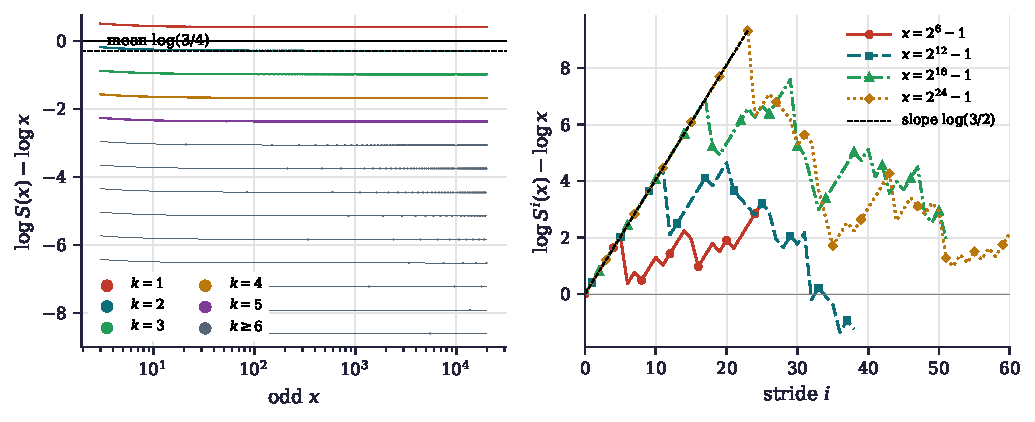
\includegraphics[width=\textwidth]{figures/ch4_stride_runs.pdf}
\caption{Left: the stride increment $\log S(x)-\log x$ for every odd
$x\le20000$, coloured by $k=\vt(3x+1)$.  Each point lies on the curve
$\log(3+1/x)-k\log2$ of its $k$ (thin lines), and only $k=1$ lies above zero; the dashed
line is the model mean $\log(3/4)$.  Right: the log trajectory
$\log S^{i}(x)-\log x$ for $x=2^{j}-1$ with $j=6,12,18,24$.  Each climbs in a
straight run of $j-1$ ascending strides, close to the black dashed line of slope
$\log(3/2)$, before the first descent (\cref{prop:ch4:chain}).}
\label{fig:ch4:runs}
\end{figure}

\section{No monotone strong Lyapunov function for a single stride}\label{sec:ch4:nolyap}

\Cref{thm:stride} already contains the first obstruction.  If half of all odd
integers ascend, then no function that increases with $x$ can decrease along
every stride.

\begin{theorem}[Impossibility of a monotone single stride strong Lyapunov function]
\label{thm:nolyapunov}
Let $W$ be a strictly increasing function from the odd positive integers to
$(0,\infty)$, and let $\rho\le1$.  Then $W(S(x))>\rho\,W(x)$ for every
$x\equiv3\pmod4$.  In particular no strictly increasing $W$ is a strict or
strong Lyapunov function\index{Lyapunov function} for $(S,\{1\})$, and the set of odd integers on which
it fails contains the residue class $3\bmod4$, which has natural density $\tfrac12$ among the odd integers; for $\rho=1$ it is exactly this class.
\end{theorem}

\begin{proof}
For $x\equiv3\pmod4$, \cref{thm:stride}(iii) gives $S(x)>x$, so
$W(S(x))>W(x)\ge\rho W(x)$.  The residue class $3\bmod4$ contains half of the
odd integers.
For $\rho=1$ the inequality $W(S(x))\le W(x)$ holds at every $x\equiv1\pmod4$ with $x\ge5$, since there $S(x)<x$ by \cref{thm:stride}(ii).
\end{proof}

The same argument covers every nondecreasing $W$ with values in $(0,\infty)$, since then $W(S(x))\ge W(x)>\rho W(x)$ on the class $x\equiv3\pmod4$ when $\rho<1$, and $W(S(x))<W(x)$ fails there when $\rho=1$; and no nonincreasing $W$ works either, since $S(5)=1<5$ gives $W(S(5))\ge W(5)$. So no monotone $W$ is a strict or strong Lyapunov function for $(S,\{1\})$.

The proof is two lines, and the theorem is correspondingly robust.  It does
not depend on the form of $W$, only on its monotonicity, and it does not
depend on any probabilistic model.  It applies to $W=\log x$, to $W=x^p$ for
every $p>0$, to $W=(\log x)^2$ on $x\ge3$, and to any composite of these with
an increasing function.  Nor is it a boundary effect: the failures are not
confined to small $x$ or to a thin set, but occupy a full residue class.

\begin{remark}[Rate of ascent]\label{rem:ch4:ascentrate}
On the ascending class the increment is
$\log(S(x)/x)=\log(3/2+1/(2x))$, which decreases to $\log(3/2)\approx0.405$
as $x\to\infty$.  So the absolute ascent per stride is bounded below by
$\log(3/2)$ uniformly, while the relative ascent
\[
  \frac{\log S(x)}{\log x}=1+\frac{\log(3/2)}{\log x}+O\Bigl(\frac{1}{x\log x}\Bigr)
\]
tends to $1$ from above.  A reparametrization $W=\phi(\log x)$ with $\phi$
increasing converts this into $W(S(x))/W(x)=\phi(\log x+\log(3/2)+o(1))/\phi(\log x)$,
which exceeds $1$ for every increasing $\phi$; no choice of $\phi$ pushes the
ratio below $1$, and the most one can arrange is that it tends to $1$, as it
does for $\phi(u)=u^2$.
\end{remark}

\begin{remark}[Monotonicity is the essential hypothesis]\label{rem:ch4:monotone}
\Cref{thm:nolyapunov} is sharp in the following sense.  If one drops
monotonicity, then by \cref{rem:ch4:exists} a strong Lyapunov function bounded
away from zero exists if and only if the conjecture is true; if it is, the function $2^{\sigma_S(x)}$ is one.
The theorem therefore draws a precise line.  Certificates that increase with the
size of $x$ are impossible; certificates\index{certificate} that see the arithmetic of $x$ are
possible in principle but are, at present, equivalent to the conjecture.  Any
viable certificate must depend on $x$ through more than its magnitude, for
instance through its residues modulo powers of $2$ and $3$, which is where
\cref{chap:parity,chap:stochastic} and \cref{chap:divergence} look for
structure.
\end{remark}

\section{Two stride compositions}\label{sec:ch4:twostride}

A natural response to \cref{thm:nolyapunov} is to look at several strides at
once.  Every ascent is followed sooner or later by a descent, and one might
hope that over two strides the descents always win.  They do not, and the
two stride case can be analysed completely.

For odd $x$ write $k_1=\vt(3x+1)$, $y=S(x)$ and $k_2=\vt(3y+1)$.  Expanding
$S(y)=(3y+1)/2^{k_2}$ gives
\begin{equation}\label{eq:ch4:twostride}
  S^{(2)}(x)=\frac{9x+3+2^{k_1}}{2^{k_1+k_2}} .
\end{equation}

\begin{lemma}[Two stride residue classes]\label{lem:ch4:tworesidue}
For integers $a,b\ge1$, the set of odd $x$ with $k_1=a$ and $k_2=b$ is a
single residue class modulo $2^{a+b+1}$.  Consequently it has natural density
$2^{-(a+b)}$ among the odd integers.
\end{lemma}

\begin{proof}
The condition $k_1=a$ says $3x+1\equiv2^a\pmod{2^{a+1}}$, and since $3$ is
invertible modulo $2^{a+1}$ this is a single class $x\equiv x_0\pmod{2^{a+1}}$.
Write $x=x_0+2^{a+1}t$.  Then $S(x)=(3x_0+1)/2^a+6t=y_0+2\cdot3t$ with $y_0$
odd.  As $t$ runs over a complete residue system modulo $2^{b}$, so does $3t$,
and hence $S(x)$ runs over all odd residues modulo $2^{b+1}$, each exactly once.
The condition $k_2=b$ selects one odd residue class of $S(x)$ modulo $2^{b+1}$,
hence one class of $t$ modulo $2^b$, hence one class of $x$ modulo $2^{a+b+1}$.
There are $2^{a+b}$ odd classes modulo $2^{a+b+1}$, which gives the density.
\end{proof}

The lemma is the two stride case of the parity vector\index{parity vector} bijection of
\cref{thm:terras}, written in the language of strides.

\begin{proposition}[Exact two stride behaviour]\label{prop:ch4:twostride}
Let $x\ge3$ be odd.
\begin{enumerate}[label=(\roman*)]
\item $S^{(2)}(x)<x$ if and only if $k_1+k_2\ge4$.
\item The odd integers with a two stride descent have natural density exactly
  $\tfrac12$ among the odd integers.
\item $\displaystyle\max_{x\ge3\text{ odd}}\bigl(\log S^{(2)}(x)-\log x\bigr)
  =\log\frac{17}{7}\approx0.8873$, attained only at $x=7$, where
  $S(7)=11$ and $S^{(2)}(7)=17$.
\end{enumerate}
\end{proposition}

\begin{proof}
Put $s=k_1+k_2\ge2$.  If $s\le3$ then $2^{k_1}\ge2$ and \eqref{eq:ch4:twostride}
gives $S^{(2)}(x)\ge(9x+5)/8>x$.  If $s\ge4$ then $2^{k_1}\le2^{s-1}$, so it
suffices to check $9x+3+2^{s-1}<2^sx$, that is $(2^s-9)x>3+2^{s-1}$.  For
$s=4$ this reads $7x>11$, true for $x\ge3$; for $s\ge5$ the left side is at
least $3(2^s-9)$ and $3\cdot2^s-27-3-2^{s-1}=\tfrac52\,2^s-30>0$.  This
proves (i).

For (ii), by (i) and \cref{lem:ch4:tworesidue} the ascending set is the union
of the classes $(k_1,k_2)\in\{(1,1),(1,2),(2,1)\}$, of total density
$2^{-2}+2^{-3}+2^{-3}=\tfrac12$.

For (iii), if $(k_1,k_2)=(1,1)$ then $S^{(2)}(x)/x=(9x+5)/(4x)$, which
decreases in $x$.  The condition $k_1=1$ means $x\equiv3\pmod4$, and then
$k_2=1$ means $(3x+1)/2\equiv3\pmod4$, that is $x\equiv7\pmod8$.  The least
such $x$ is $7$, giving the ratio $68/28=17/7$.  If $s=3$ the ratio is at most
$(9x+7)/(8x)\le34/24<17/7$, and if $s\ge4$ the ratio is below $1$.
\end{proof}

Under the Geometric$(\tfrac12)$ model the two stride increment is
$\Delta_1+\Delta_2$ with mean $2\log(3/4)\approx-0.5754$, and the probability
that $k_1+k_2\le3$ is $\tfrac14+\tfrac18+\tfrac18=\tfrac12$, so the model
reproduces part (ii) exactly.  The arithmetic agrees with it at every scale we
have examined.  Over the odd $x$ with $3\le x\le20001$ the script \texttt{ch4\_ch5\_numbers.py} (see
\cref{app:code}) finds the two stride increment negative for exactly half of
the $10000$ starting values, with mean increment $-0.574681$ against the
theoretical $2\log(3/4)=-0.575364$, and largest ascent $0.8873$ at $x=7$.
Extending the scan to all odd $x$ with $3\le x<2\times10^6$ gives a descending fraction of
$0.4999995$ and mean $-0.575359$; the residual discrepancy from $\tfrac12$ is
the edge effect of truncating the residue classes of
\cref{lem:ch4:tworesidue}.

Averaging over two strides therefore doubles the mean descent without
reducing the proportion of ascending starting points at all.  The left panel
of \cref{fig:ch4:phase} shows the same phenomenon for the two step composition
of the accelerated map\index{accelerated map}, where the split is by $x\bmod4$: the class
$x\equiv1\pmod4$ falls on the curve $\log(3/4+1/(4x))$ and the class
$x\equiv3\pmod4$ on $\log(9/4+5/(4x))$, about $0.81$ above zero.
The right panel follows whole orbits of $T$ in the phase coordinates $(\log x_n,\log x_{n+1})$: every step lands on the lower branch $\log x_{n+1}=\log x_n-\log2$ or just above the upper branch $\log x_{n+1}=\log x_n+\log(3/2)$, and the orbit of $27$, for example, takes the upper branch $41$ times and the lower one only $29$ times, yet descends, because a halving moves $\log x$ by more than an odd step does.

\begin{figure}[t]
\centering
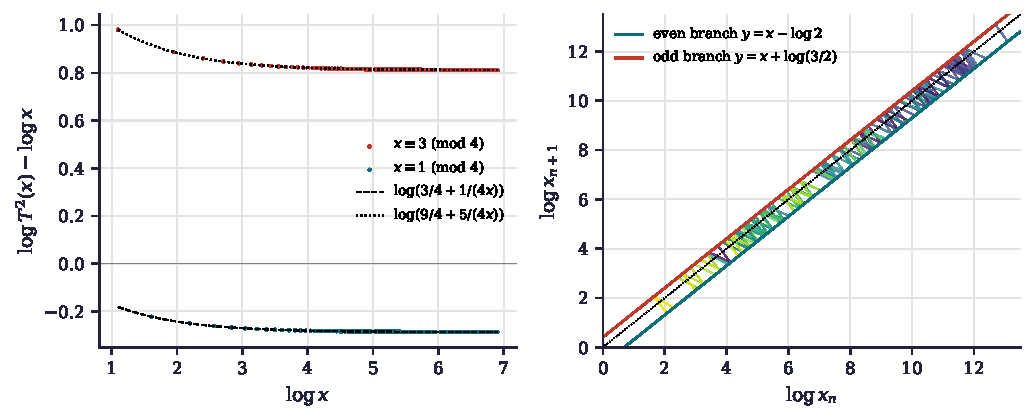
\includegraphics[width=\textwidth]{figures/ch4_phase.pdf}
\caption{Left: two step increment $\log T^{2}(x)-\log x$ of the accelerated
map for odd $x\le1000$.  The class $x\equiv1\pmod4$ descends, on the curve
$\log(3/4+1/(4x))$, which lies above its limit $\log(3/4)$; the class
$x\equiv3\pmod4$ ascends, on the curve $\log(9/4+5/(4x))$.  Right: phase
portrait in log coordinates for the accelerated orbits of $27$, $97$, $255$,
$703$ and $6171$, coloured by the fraction of the orbit elapsed.  Every step
lands on one of the two branches $\log x_{n+1}=\log x_n-\log2$ and
$\log x_{n+1}\approx\log x_n+\log(3/2)$.}
\label{fig:ch4:phase}
\end{figure}

\section{The log squared candidate}\label{sec:ch4:logsq}

A second natural response to \cref{thm:nolyapunov} is to change the potential.
Quadratic potentials are the default in optimization, and the obvious
candidate is $W(x)=(\log x)^2$.  Its behaviour illustrates, more sharply than
any other example, the difference between descent in expectation and descent
at every point.

Write $u=\log x$ and $\Delta=\log S(x)-\log x$.  Then, identically,
\begin{equation}\label{eq:ch4:logsq}
  (\log S(x))^2-(\log x)^2=(u+\Delta)^2-u^2=2u\,\Delta+\Delta^2 .
\end{equation}
Now take expectations under the stride model, in which $\Delta=\log3-k\log2$
with $k$ Geometric$(\tfrac12)$ and independent of $u$.  Then
$\E[\Delta]=\log(3/4)$ and $\Var(\Delta)=(\log2)^2\Var(k)=2(\log2)^2$, so
$\E[\Delta^2]=2(\log2)^2+(\log(3/4))^2\approx1.0437$ and
\begin{equation}\label{eq:ch4:logsqmean}
\begin{aligned}
  \E\bigl[(\log S(x))^2-(\log x)^2\bigr]
  &=2\log(3/4)\,\log x+\E[\Delta^2]\\
  &\approx-0.5754\,\log x+1.0437 .
\end{aligned}
\end{equation}
This is negative as soon as $\log x>\E[\Delta^2]/(2|\log(3/4)|)\approx1.814$,
that is for $x\ge7$, and the expected decrease grows without bound in
$\log x$.  For $J$ strides the same computation gives
$2J\log(3/4)\log x+\E[(\Delta_1+\dots+\Delta_J)^2]$, negative for
$\log x\gtrsim1.958$ when $J=2$.

One might read \eqref{eq:ch4:logsqmean} as saying that $(\log x)^2$
is a ``super Lyapunov'' function whose descent accelerates as the orbit grows.
That reading is wrong in two separate ways.

\begin{remark}[A tempting but false argument]\label{rem:ch4:logsqpitfall}
First, \eqref{eq:ch4:logsqmean} is a statement about the model, not about the
map.  For an individual $x\equiv3\pmod4$ the increment $\Delta$ is positive,
and \eqref{eq:ch4:logsq} gives $(\log S(x))^2-(\log x)^2=2u\Delta+\Delta^2>0$:
the potential increases, and by \emph{more} the larger $x$ is.  The expected
decrease and the pointwise increase both grow linearly in $\log x$; the first
averages the increase on the ascending half with the decreases on the descending half, which are larger on average.  Since
$(\log x)^2$ is increasing on $x\ge1$, \cref{thm:nolyapunov} applies to it
directly, and \cref{cor:ch4:multistride} below extends the failure to any
fixed number of strides.

Second, even in the model the growth of the absolute decrease is an artefact
of the scale of $W$.  The relative change is
\[
  \frac{\E[W(S(x))]}{W(x)}-1=\frac{2\log(3/4)}{\log x}+\frac{\E[\Delta^2]}{(\log x)^2},
\]
which tends to $0$.  Measured as a contraction factor, which is what a strong
Lyapunov function\index{Lyapunov function} requires, $(\log x)^2$ contracts \emph{less} as $x$ grows,
not more.  There is no constant $\rho<1$ with
$\E[W(S(x))]\le\rho W(x)$ for all large $x$ even in the model.
\end{remark}

The lesson generalizes.  For any potential of the form $\phi(\log x)$ with
$\phi$ smooth and increasing, a Taylor expansion gives an expected change
$\phi'(u)\log(3/4)+\tfrac12\phi''(u)\E[\Delta^2]+\cdots$, and one can choose
$\phi$ to make this negative or to make it grow.  None of these choices
touches the pointwise behaviour, which is governed by the sign of $\Delta$
alone.

\section{Multi stride certificates and chained ascents}\label{sec:ch4:multi}

The last hope for a monotone certificate\index{certificate} is to fix a number of strides $J$ and
ask for $W(S^{(J)}(x))\le\rho\,W(x)$ for all odd $x\ge3$.  For $J=2$ this
fails by \cref{prop:ch4:twostride}.  The following proposition shows that it
fails for every $J$, for an explicit and simple reason: ascending strides can
be chained to any length, and the starting points that produce long chains
are completely explicit.

\begin{proposition}[Chained ascents]\label{prop:ch4:chain}
Let $x$ be odd and write $x+1=2^{j}q$ with $q$ odd, so that $j=\vt(x+1)\ge1$.
Then for $0\le i\le j-1$,
\begin{equation}\label{eq:ch4:chain}
  S^{(i)}(x)=3^{i}\,2^{\,j-i}\,q-1 ,
\end{equation}
the first $j-1$ strides from $x$ all have $k=1$ and ascend, and the $j$th
stride has $k\ge2$ and, if $x\ge3$, descends.  In other words, the length of the initial
run of ascending strides from $x$ is exactly $\vt(x+1)-1$.
\end{proposition}

\begin{proof}
We prove \eqref{eq:ch4:chain} by induction on $i$; the case $i=0$ is the
definition of $j$ and $q$.  Suppose \eqref{eq:ch4:chain} holds for some
$i\le j-2$, and put $z=S^{(i)}(x)=3^i2^{j-i}q-1$.  Since $j-i\ge2$, $z\equiv-1
\equiv3\pmod4$, so by \cref{thm:stride}(iii) the next stride has $k=1$ and
\[
  S(z)=\frac{3z+1}{2}=\frac{3^{i+1}2^{j-i}q-2}{2}=3^{i+1}2^{\,j-i-1}q-1,
\]
which is \eqref{eq:ch4:chain} for $i+1$.  This shows that strides
$1,\dots,j-1$ have $k=1$.  For the $j$th stride, $z=S^{(j-1)}(x)=2\cdot3^{j-1}q-1$
with $3^{j-1}q$ odd, so $z\equiv1\pmod4$ and the stride has $k\ge2$, hence,
since $z\ge3$ when $x\ge3$, descends by \cref{thm:stride}(ii) (for $x=1$ the stride is $S(1)=1$).
\end{proof}

Formula \eqref{eq:ch4:chain} is the identity of \cref{rem:ch2:pitfall} written
for $S$, and it is classical: see Hercher\index{Hercher, C.}~\cite[Lemma~8]{hercher2023},
who cites Terras\index{Terras, R.}~\cite{terras1976} for it.
For example, $x=7=2^3-1$ gives $j=3$, $q=1$, and indeed $S(7)=11=3\cdot2^2-1$,
$S^{(2)}(7)=17=9\cdot2-1$, after which $S(17)=13$ descends.  The integer
$x=2^{24}-1$ climbs through $23$ consecutive ascents, multiplying by nearly
$3/2$ each time, before its first descent; the right panel of
\cref{fig:ch4:runs} shows this and three shorter chains.

\begin{corollary}[No fixed horizon monotone certificate]\label{cor:ch4:multistride}
Fix $J\ge1$, $\rho\le1$ and a strictly increasing $W$ from the odd positive
integers to $(0,\infty)$.  Then $W(S^{(J)}(x))>\rho\,W(x)$ for every odd
$x\equiv-1\pmod{2^{J+1}}$, that is for every $x=2^{J+1}q-1$ with $q\ge1$.
This set is infinite and has natural density $2^{-J}$ among the odd integers.
Moreover, along it,
\[
  \frac{S^{(J)}(x)}{x}\;\longrightarrow\;\Bigl(\frac32\Bigr)^{J}
  \qquad(q\to\infty).
\]
\end{corollary}

\begin{proof}
If $x\equiv-1\pmod{2^{J+1}}$ then $\vt(x+1)\ge J+1$, so by
\cref{prop:ch4:chain} the first $J$ strides all ascend and
$S^{(J)}(x)>x$; monotonicity of $W$ finishes the argument.  The residue class
$-1\bmod2^{J+1}$ is one of the $2^{J}$ odd classes modulo $2^{J+1}$.  For the
limit, write $x+1=2^{j}q'$ with $j\ge J+1$ and $q'$ odd; then
\eqref{eq:ch4:chain} with $i=J$ gives
$S^{(J)}(x)/x=(3^J2^{j-J}q'-1)/(2^jq'-1)$, which tends to $(3/2)^J$ as $x$
grows within the class.
\end{proof}

The corollary is the precise content of the slogan that ``chaining ascending
strides defeats every monotone multi stride certificate''.  It says more than that each
monotone fixed horizon certificate fails somewhere: it fails on a full residue class,
and on that class $\log x$ grows over the horizon by an amount
approaching $J\log(3/2)$, which is unbounded as $J$ grows.  The
horizon cannot be chosen to outrun the chains, because the chains are as long
as the $2$ adic valuation of $x+1$, and that valuation is unbounded.
As after \cref{thm:nolyapunov}, nondecreasing $W$ are covered by the same argument, and nonincreasing $W$ fail at $x=5$, since $S^{(J)}(5)=1$ for every $J\ge1$.

\begin{remark}[How the obstruction is distributed]\label{rem:ch4:distribution}
The initial run length $\vt(x+1)-1$ has, among odd $x$, natural density
$2^{-(r+1)}$ of being equal to $r$, so long chains are rare but not negligible
in any fixed proportion: a fraction $2^{-J}$ of odd integers defeats every
$J$ stride certificate that increases with $x$.  This is the same Geometric law as the halving
exponent $k$ in \cref{prop:geom}, and for the same reason; both are statements
about the $2$ adic digits of $x$.  It is also the reason the obstruction is not
merely an artefact of small numbers.  The class $x\equiv-1\pmod{2^{J+1}}$
contains integers of every size.
\end{remark}

\section{Majorization minimization for the log potential}\label{sec:ch4:mm}

We turn now from Lyapunov functions\index{Lyapunov function} to a second piece of optimization
technology, the majorization\index{majorization} minimization (MM) principle of Lange\index{Lange, K.}, Hunter\index{Hunter, D. R.} and
Yang\index{Yang, I.}~\cite{lange2000} and Hunter and Lange~\cite{hunter2004}, and ask whether
it can supply a descent certificate\index{certificate} that the direct approach cannot.  The
answer is no, but the reason is illuminating and connects back to the
martingale\index{martingale} duality of \cref{thm:martingale}.

Recall the principle.  To minimize an objective $V$, one constructs at the
current point $x_n$ a surrogate $g(\cdot\mid x_n)$ satisfying
\emph{domination}, $g(y\mid x_n)\ge V(y)$ for all $y$, and \emph{tangency},
$g(x_n\mid x_n)=V(x_n)$.  Any move that does not increase the surrogate then
does not increase the objective, since
$V(x_{n+1})\le g(x_{n+1}\mid x_n)\le g(x_n\mid x_n)=V(x_n)$.  More generally,
for any move, the change in the objective is bounded by the change in the
surrogate.

\subsection{The linear majorizer}

Take the objective to be $V(x)=\log x$, which on the positive integers is
minimized exactly at $x=1$.  Since $\log$ is concave, its tangent line at any
$x_n>0$ lies above it:
\begin{equation}\label{eq:ch4:major}
  \log y\;\le\;g(y\mid x_n):=\log x_n+\frac{y-x_n}{x_n},\qquad y>0,
\end{equation}
with equality at $y=x_n$.  Both defining properties hold, so $g$ is a
majorizer\index{majorization} in the sense of the MM literature.

\begin{remark}[A pitfall: majorizing $-\log$]\label{rem:ch4:minuslog}
It is easy to set the problem up the wrong way round.  If one takes the
objective to be $-\log x$ and asserts that its tangent line majorizes it, the
inequality is reversed: $-\log$ is convex, so its tangent lies \emph{below} it
and is a minorizer, and nothing can be concluded about descent.  The
formulation also has the wrong target, since $-\log x$ is minimized at
$x=\infty$, not at $x=1$.  With $V=\log$ as in \eqref{eq:ch4:major}, both the
direction of the inequality and the location of the minimum are correct.
\end{remark}

Domination and tangency give the following bound\index{MM algorithm}: the true objective
improves by at least as much as the surrogate.  It holds at every step, in both
parities.

\begin{proposition}[Tangent line bound for $T_0$]\label{prop:mmdescent}
For every $x\in\N$,
\[
  V(T_0(x))-V(x)\;\le\;g(T_0(x)\mid x)-g(x\mid x)
  =\begin{cases}
     -\tfrac12, & x\text{ even},\\[2pt]
     2+\tfrac1x, & x\text{ odd}.
   \end{cases}
\]
\end{proposition}

\begin{proof}
Apply \eqref{eq:ch4:major} with $x_n=x$ and $y=T_0(x)$, and use
$g(x\mid x)=V(x)$.  For even $x$ the surrogate increment is
$(x/2-x)/x=-\tfrac12$, while the true increment is $-\log2\approx-0.693$.  For
odd $x$ the surrogate increment is $(3x+1-x)/x=2+1/x$, while the true
increment is $\log(3+1/x)\le\log(10/3)\approx1.204$ for $x\ge3$.
\end{proof}

The inequality uses only domination and tangency, so it holds for any next
iterate whatever; $T_0(x)$ is not obtained by minimizing $g(\cdot\mid x)$, and
the Collatz map is not an MM iteration in the usual sense.  Worse, the bound
certifies nothing.

\begin{proposition}[The linear majorizer cannot certify descent]\label{prop:mmfails}
Under the stochastic model for the standard map\index{standard map}, in which the parities
form the renewal\index{renewal theory} chain $(B_n)$ of \cref{thm:autocorr} and a step is odd with
stationary probability $\tfrac13$, the mean surrogate increment per step of
$T_0$ is
\[
  \tfrac13\cdot2+\tfrac23\cdot\bigl(-\tfrac12\bigr)=+\tfrac13\;>\;0,
\]
up to the $O(1/x)$ term, whereas the mean true increment per step is
$\tfrac13\log3-\tfrac23\log2=\tfrac13\log(3/4)\approx-0.0959<0$.  Per Syracuse
stride, the mean surrogate increment is $+1$ and the mean true increment is
$\log(3/4)\approx-0.2877$.
\end{proposition}

\begin{proof}
The per step values follow from \cref{prop:mmdescent} and the stationary
parity frequencies.  A stride consists of one odd step followed by $k$ even
steps, so the surrogate increments summed over a stride equal
$2+1/x-k/2$, with mean $2-\E[k]/2=1$ up to $O(1/x)$; the true increment over
the stride is \eqref{eq:ch4:stride}, with mean $\log3-2\log2$ in the model.
\end{proof}

A word on levels, since three drifts are now in play.  The figure
$\tfrac13\log(3/4)$ is the drift\index{drift} per step of $T_0$; the drift per step of the
accelerated map\index{accelerated map} $T$ is $\ds=\log(\sqrt3/2)=\tfrac12\log(3/4)\approx-0.1438$;
and the drift per Syracuse stride is $\log(3/4)$.  They are the same quantity
measured against clocks that tick on average three times, twice and once per
stride.  The comparison in \cref{prop:mmfails} is between quantities measured
on the same clock, and the sign disagreement does not depend on which clock is
used.

In the model, therefore, the surrogate drifts upward while the potential
drifts downward, and iterating the majorization will never produce a descent
certificate\index{certificate}.  The reason is visible in \eqref{eq:ch4:major}: the tangent line
is an accurate upper bound only for $y$ close to $x_n$, and the odd step
multiplies by three.  At a multiplicative jump of that size the linear bound
gives $2$ where the logarithm gives $\log3\approx1.10$, an overestimate by a
factor of about $1.8$, which is more than enough to swamp the halvings.

\subsection{Why the linear surrogate sees no drift}

There is a cleaner way to say what goes wrong, which explains why no
tinkering with the linear surrogate can help.  At the level of strides, the
surrogate increment of \eqref{eq:ch4:major} is
\[
  g(S(x)\mid x)-g(x\mid x)=\frac{S(x)}{x}-1=\frac{3+1/x}{2^{k}}-1 .
\]
Under the Geometric$(\tfrac12)$ law, $\E[2^{-k}]=\sum_{j\ge1}4^{-j}=\tfrac13$,
so the mean surrogate increment per stride, computed directly at the stride
level, is
\begin{equation}\label{eq:ch4:martsurrogate}
  \E\Bigl[\frac{S(x)}{x}\Bigr]-1=\frac{3+1/x}{3}-1=\frac{1}{3x} .
\end{equation}
Up to the vanishing term $1/(3x)$, the stride ratio $S(x)/x$ has mean exactly
one: the Syracuse iterates form a multiplicative martingale\index{martingale} in the model, just
as the accelerated iterates do in \cref{thm:martingale}.  (The value $+1$ in
\cref{prop:mmfails} is larger because there the majorizer\index{majorization} is recentred at
every intermediate step, and each recentring adds a further Jensen gap\index{Jensen inequality}.)  A
linear surrogate measures the expected change of $x$ itself, which is zero to
first order, and is therefore structurally blind to the descent of $\log x$,
which is the Jensen defect
$\E[\log(S(x)/x)]-\log\E[S(x)/x]\approx\log(3/4)$.  This is the martingale
duality of \cref{chap:stochastic} seen through the MM lens: any surrogate that
is affine in $x$ inherits the drift\index{drift} of the martingale, which is nil.

\subsection{Power majorizers and the Wald root}

If the linear surrogate is too loose under multiplication, one can ask for a
surrogate that is tighter under multiplication.  A natural family is obtained
from the inequality $\log r\le(r^{p}-1)/p$, valid for $r>0$ and $p>0$ with
equality at $r=1$.  For $0<p\le1$ define
\begin{equation}\label{eq:ch4:power}
  g_p(y\mid x)=\log x+\frac{(y/x)^{p}-1}{p}.
\end{equation}
Each $g_p$ dominates $\log y$ and is tangent to it at $y=x$, so each is an MM
majorizer\index{majorization} of $V=\log$; the case $p=1$ is the linear majorizer
\eqref{eq:ch4:major}, and as $p\downarrow0$ the surrogate tends to $\log y$
itself.  Its stride increment is $((S(x)/x)^{p}-1)/p$, and its mean under the
stride model involves the moment generating function of the log increment
$\Delta=\log3-k\log2$:
\begin{equation}\label{eq:ch4:mgf}
  M(p):=\E\bigl[e^{p\Delta}\bigr]=3^{p}\sum_{j\ge1}2^{-j}2^{-pj}
  =\frac{3^{p}}{2^{1+p}-1}.
\end{equation}

\begin{proposition}[Power majorizers]\label{prop:ch4:power}
Under the stride model, the mean stride increment of the surrogate
\eqref{eq:ch4:power}, ignoring the $1/x$ correction, is $(M(p)-1)/p$, and:
\begin{enumerate}[label=(\roman*)]
\item $M(0)=M(1)=1$, and $M(p)<1$ for $0<p<1$;
\item $p\mapsto(M(p)-1)/p$ is increasing on $(0,1]$, tends to
  $\E[\Delta]=\log(3/4)$ as $p\downarrow0$, and equals $0$ at $p=1$.
\end{enumerate}
In particular every power majorizer with $0<p<1$ has strictly negative mean
surrogate increment, and the linear majorizer $p=1$ sits exactly on the
boundary.
\end{proposition}

\begin{proof}
From \eqref{eq:ch4:mgf}, $M(0)=1/(2-1)=1$ and $M(1)=3/(4-1)=1$.  A moment
generating function of a nondegenerate random variable is strictly convex, so
$M<1$ strictly between its two roots of $M=1$.  For (ii), $(M(p)-1)/p$ is the
slope of the chord of the convex function $M$ from $0$ to $p$, which is
nondecreasing in $p$ and tends to $M'(0)=\E[\Delta]$ as $p\downarrow0$; strict
convexity makes it increasing.
\end{proof}

Numerically, $M(\tfrac12)=\sqrt3/(2\sqrt2-1)\approx0.9473$, so the surrogate
$g_{1/2}$ has mean stride increment about $-0.105$, against $-0.181$ for
$p=\tfrac14$ and $-0.047$ for $p=\tfrac34$.  The family interpolates
monotonically between the true drift\index{drift} $\log(3/4)$ at $p=0$ and the martingale\index{martingale}
drift $0$ at $p=1$.  The point $p=1$ is the nonzero root of $M(p)=1$, the
\emph{Wald root} of the stride walk; it is the stride counterpart of the Wald
root $1$ of the accelerated map (\cref{thm:martingale}), and it is not a coincidence that
it falls exactly on the linear majorizer.  The equation $M(p)=1$ is the
statement that $e^{p\log x}=x^{p}$ is a martingale, and at
$p=1$ that is the martingale property of $x$ itself.  Including the exact
correction, $M_x(p)=(3+1/x)^{p}/(2^{1+p}-1)$, so $M_x(1)=1+1/(3x)$ as in
\eqref{eq:ch4:martsurrogate}, and for each $p<1$ the mean surrogate increment
is negative for all sufficiently large $x$.

Equivalently, for $0<p<1$ the function $W_p(x)=x^{p}$ is a supermartingale\index{supermartingale}
along strides in the model, $\E[W_p(S(x))]\approx M(p)\,W_p(x)$ with
$M(p)<1$: in the model it is even a geometric Foster function.

\subsection{What a multiplicatively tight majorizer would need}

\Cref{prop:ch4:power} shows that tightening the majorizer\index{majorization} under
multiplication does exactly what one would hope at the level of the model: as
soon as the surrogate curves below the tangent line, its mean increment turns
negative.  It also shows what it cannot do.  Every $g_p$ is an increasing
function of $y$, so the surrogate increment is positive whenever $S(x)>x$,
that is on the whole residue class $x\equiv3\pmod4$; and $W_p=x^{p}$ is
strictly increasing, so \cref{thm:nolyapunov} and \cref{cor:ch4:multistride}
apply to it without change.  A majorizer that certified descent pointwise
would have to satisfy three requirements at once.
\begin{enumerate}[label=(\alph*)]
\item It must dominate $\log$ and be tangent to it, so that surrogate descent
  implies true descent.
\item It must be tight enough under multiplication that its drift in the
  model is negative; by \cref{prop:ch4:power} this means curving below the
  linear majorizer, as $g_p$ does for $p<1$.
\item Its increment must be negative at every odd $x$, including those with
  $k=1$, and over every horizon, including the chains of
  \cref{prop:ch4:chain}.
\end{enumerate}
Requirements (a) and (b) are compatible and are met by the power family.
Requirement (c) is incompatible with (a) for every surrogate, because on the
ascending class $\log S(x)>\log x$, and domination and tangency then force the
surrogate increment up to at least $\log S(x)-\log x>0$, as in
\cref{prop:mmdescent}.  No majorizer of $\log$ can meet all three; a certificate
of this kind would have to majorize a potential other than $\log x$, one that
depends on the arithmetic of $x$ and not merely on its magnitude, and by
\cref{rem:ch4:monotone} constructing one is, as far as anyone
knows, as hard as the conjecture.  We do not know of one, and we regard the
search for an MM certificate\index{certificate} of this kind as a reformulation of the problem
rather than a route around it.

\section*{Notes}

Lyapunov's 1892 memoir on the stability of motion, available in English translation~\cite{lyapunov1992}, is the origin of the method;
for discrete systems, including the invariance principle, see
LaSalle~\cite{lasalle1986}.  Foster's criterion\index{Foster criterion} appeared in
Foster~\cite{foster1953}; the systematic theory of drift\index{drift} conditions, including
geometric drift and its relation to geometric ergodicity, is in Meyn and
Tweedie~\cite{meyn1993}, whose second edition (Cambridge University Press,
2009) adds a new prologue and, by Meyn, commentary and an epilogue on later developments.  The equivalence of
the conjecture with finiteness of all stopping times\index{stopping time}
(\cref{prop:ch4:eventual}) is folklore and is implicit in
Terras\index{Terras, R.}~\cite{terras1976}; see also the survey of Lagarias\index{Lagarias, J. C.}~\cite{lagarias1985}
and the collection~\cite{lagarias2010}.  The stride descent theorem is a direct
computation from the definition of $S$, and the impossibility of a monotone
certificate\index{certificate} at any fixed stride depth follows in one line from the chained
ascent formula (\cref{prop:ch4:chain}), which is the classical identity
$T^{(J)}(a2^{J}-1)=a3^{J}-1$ for the accelerated map written for $S$; see
Hercher\index{Hercher, C.}~\cite[Lemma~8]{hercher2023}, who cites Terras~\cite{terras1976} for it.
The observation that $x\equiv-1\pmod{2^{j}}$ produces long ascending runs
appears in many expositions of the Terras parity vector\index{parity vector}.  The exact two
stride analysis (\cref{prop:ch4:twostride}) and the power majorizer\index{majorization}s
(\cref{prop:ch4:power}) are presented here for the first time in this form.
For the MM principle see Lange, Hunter and Yang~\cite{lange2000}, Hunter and
Lange~\cite{hunter2004} and, for incremental versions,
Mairal\index{Mairal, J.}~\cite{mairal2015}.  The role of Wald's identity\index{Wald identity}, of the overshoot (\cref{prop:ch4:passage}) and of the root of the
moment generating function in random walks with negative drift is standard;
in the Collatz setting the corresponding computations for the accelerated map\index{accelerated map}
are in \cref{chap:stochastic}.

\section*{Exercises}

\begin{exercise}
Show that for odd $x$ and $j\ge1$, $\vt(3x+1)=j$ exactly when $x$ lies in a
single residue class modulo $2^{j+1}$, and find this class for $j=1,2,3,4$.
Deduce that $\vt(3x+1)=1$ if and only if $x\equiv3\pmod4$.
\end{exercise}

\begin{exercise}
Prove \eqref{eq:ch4:twostride}. The two stride ascending set of
\cref{prop:ch4:twostride} is a union of residue classes modulo $16$; find
them, and check that there are exactly four of them among
the eight odd classes.
\end{exercise}

\begin{exercise}
Let $x\equiv3\pmod4$ and put $j=\vt(x+1)$, so that $j\ge2$.  Use \cref{prop:ch4:chain} to show that
$\log S^{(j-1)}(x)-\log x>(j-1)\log(3/2)$.  Conclude that for every $B>0$
there is an odd $x$ and a number of strides $J$ with
$\log S^{(J)}(x)-\log x>B$, so that no bound on the cumulative ascent holds
uniformly in the horizon.
\end{exercise}

\begin{exercise}
Using the Geometric$(\tfrac12)$ law, compute $M(p)=\E[e^{p\Delta}]$ for the
stride increment and verify \eqref{eq:ch4:mgf}.  Repeat the computation for
the accelerated map\index{accelerated map} with the Bernoulli$(\tfrac12)$ model of
\cref{thm:martingale}, and show that its nonzero Wald root is also $1$.
Explain why both roots must equal $1$ whenever the iterates form a
multiplicative martingale\index{martingale}.
\end{exercise}

\begin{exercise}\label{ex:ch4:passage}
In the stride model, let $\tau$ be the first stride at which $\log x\le0$, and $O\ge0$ the overshoot below $0$ at time $\tau$, as in \cref{prop:ch4:passage}. Explain where the optional stopping argument in the proof of \cref{thm:ch4:foster} breaks down for $V=\log x$, and why the bound $\log x_0/|\log(3/4)|$ that it would give is never valid. For $s\ge0$ let $V_s=\log x+s$ when $\log x>0$ and $V_s=0$ when $\log x\le0$. Show that $V_s$ satisfies the drift condition with $\varepsilon=|\log(3/4)|$ at every $x$ with $\log x>0$ if and only if $s\ge2\log2$, and deduce from the hitting time bound that $\E_{x_0}[\tau]\le(\log x_0+2\log2)/|\log(3/4)|$, the upper half of \eqref{eq:ch4:fosterbound} with $\le$ in place of $<$.
\end{exercise}

\begin{exercise}
For the accelerated map $T$ and the linear majorizer\index{majorization} \eqref{eq:ch4:major},
show that the surrogate increment is $\tfrac12+\tfrac1{2x}$ for odd $x$ and
$-\tfrac12$ for even $x$, so that under the Bernoulli$(\tfrac12)$ model its
mean is $1/(4x)$.  Relate this to the martingale property in
\cref{thm:martingale}.
\end{exercise}

\chapter{Majorization and Momentum}\label{chap:momentum}

\Cref{chap:lyapunov} ended with a negative verdict on descent.  The potential
$\log x$ decreases on average along a Collatz orbit, but it does not decrease
along every stride, and no increasing function of $x$, however it is
reparametrized or majorized, can repair this.  Half of all odd integers ascend
in a single stride, and ascending strides can be chained to any length.  An
optimizer who met an iteration with these properties would not conclude that
it fails to converge.  She would conclude that it is not a descent method, and
she would reach for the other great family of first order methods, the
momentum\index{momentum} methods, whose iterates are allowed to overshoot and whose
convergence is certified by a potential that is not monotone in the objective.

This chapter takes that step.  We review the two classical momentum methods,
Polyak\index{Polyak, B. T.}'s heavy ball\index{heavy ball} method~\cite{polyak1964} and Nesterov\index{Nesterov, Yu.}\index{Nesterov acceleration}'s accelerated
gradient method~\cite{nesterov1983}, with their rates on strongly convex
quadratics and the optimal coefficient $(\sqrt\kappa-1)/(\sqrt\kappa+1)$, and
we recall the continuous time view of Su\index{Su, W.}, Boyd\index{Boyd, S.} and Cand\`es\index{Candes, E. J.@Cand\`es, E. J.}~\cite{su2016} and
Shi\index{Shi, B.}, Du\index{Du, S. S.}, Jordan\index{Jordan, M. I.} and Su~\cite{shi2022}, in which momentum is a damped
oscillator and the certificate\index{certificate} of convergence is an energy that includes a
kinetic term.  We then read the Collatz orbit in the same terms: the odd step
is a momentum injection that overshoots, and the run of halvings that follows
is the correction.  Matching the two pictures produces a small set of
constants, and the main business of the chapter is to say precisely which of
them mean something and which do not.

Three conclusions emerge.  The first is a set of stride constants
(\cref{def:nesterov}) whose ratio $\kappa\approx1.776$, the largest ascent of a
stride over its mean descent, is a ratio of step sizes and not a condition
number\index{condition number} (\cref{rem:nesterovlimits}).  The second is a cautionary
tale: mixing\index{mixing} constants defined at different levels of the iteration produces
spurious agreements (\cref{rem:ch5:mixing}).  The third is a single
number, $\beta=\lt-1=\log(3/2)/\log 2$, that turns up as an ascent to descent
ratio, as a definitional rewriting\index{rewriting system} of a pair of drift\index{drift} constants, as the
excess over one of the Ces\`aro threshold of \cref{chap:divergence}, and as a
ratio of Kullback\index{Kullback and Leibler divergence} and Leibler divergences.  These are one fact seen four
ways, and the number becomes the momentum coefficient of \cref{chap:smm}.
Parrondo\index{Parrondo paradox}'s paradox supplies an analogy along the way.

\section{Momentum methods}\label{sec:ch5:momentum}

Let $f:\R^d\to\R$ be $\mu$ strongly convex with $L$ Lipschitz gradient, and
write $\kappa=L/\mu\ge1$ for its condition number\index{condition number}.  The model case, and the
only one we need for rates, is the quadratic
\begin{equation}\label{eq:ch5:quad}
  f(x)=\tfrac12(x-x^\ast)^{\top}A(x-x^\ast),\qquad
  \mu I\preceq A\preceq LI .
\end{equation}
Gradient descent $x_{t+1}=x_t-\alpha\nabla f(x_t)$ acts on the component of
the error $e_t=x_t-x^\ast$ along an eigenvector with eigenvalue $\lambda$ by
multiplication by $1-\alpha\lambda$.  With $\alpha=1/L$ the worst component,
$\lambda=\mu$, contracts by $1-1/\kappa$ per step; with the best constant step
$\alpha=2/(L+\mu)$ the worst contraction is $(\kappa-1)/(\kappa+1)$.  Either
way the number of iterations needed to reduce the error by a factor
$\varepsilon$ is of order $\kappa\log(1/\varepsilon)$.  Momentum reduces this to
order $\sqrt\kappa\log(1/\varepsilon)$, and the square root is the whole point.

\subsection{Heavy ball}

Polyak~\cite{polyak1964} proposed adding to the gradient step a fraction of the
previous displacement,
\begin{equation}\label{eq:ch5:hb}
  x_{t+1}=x_t-\alpha\nabla f(x_t)+\beta(x_t-x_{t-1}),
\end{equation}
and showed that on the quadratic \eqref{eq:ch5:quad} the choice
\begin{equation}\label{eq:ch5:hbtune}
  \alpha=\frac{4}{(\sqrt L+\sqrt\mu)^2},\qquad
  \beta=\Bigl(\frac{\sqrt\kappa-1}{\sqrt\kappa+1}\Bigr)^2
\end{equation}
makes the spectral radius of the two step recursion equal to
$(\sqrt\kappa-1)/(\sqrt\kappa+1)$~\cite{polyak1987}, which matches the lower
bound of Nesterov\index{Nesterov acceleration} for first order methods on strongly convex quadratics in
high dimension~\cite{nesterov2004}.  The guarantee is a statement about
quadratics, and more generally about a neighbourhood of a nondegenerate
minimum.  It does not extend globally: Lessard\index{Lessard, L.}, Recht\index{Recht, B.} and
Packard\index{Packard, A.}~\cite{lessard2016} exhibit a strongly convex function on which heavy
ball with the tuning \eqref{eq:ch5:hbtune} fails to converge, settling
instead into a limit cycle.  Momentum that is too aggressive for the global geometry
can produce a limit cycle, a phrase the reader of \cref{chap:cycles} will
recognize.

\subsection{Nesterov acceleration}

Nesterov\index{Nesterov acceleration}~\cite{nesterov1983} moved the gradient evaluation to an extrapolated
point,
\begin{equation}\label{eq:ch5:nag}
  y_t=x_t+\beta_t(x_t-x_{t-1}),\qquad x_{t+1}=y_t-\alpha\nabla f(y_t).
\end{equation}
For merely convex $f$ and a momentum\index{momentum} sequence $\beta_t$ that tends to one like
$1-3/t$, with $\alpha=1/L$, the method achieves
$f(x_t)-f^\ast=O(L\|x_0-x^\ast\|^2/t^2)$, against $O(1/t)$ for gradient
descent, and this order cannot be improved by any first order method in the
worst case~\cite{nesterov2004}.  For strongly convex $f$ one uses a constant
coefficient.  The next proposition gives the optimal constant on quadratics
with a complete proof, since it is the formula that \cref{chap:smm} sets out
to avoid.

\begin{proposition}[Optimal constant momentum on quadratics]\label{prop:ch5:nagquad}
Let $f$ be the quadratic \eqref{eq:ch5:quad} with spectrum in $[\mu,L]$, and
run \eqref{eq:ch5:nag} with $\alpha=1/L$ and constant $\beta\in[0,1)$.  On the
eigendirection with eigenvalue $\lambda$, put $a=\lambda/L\in[1/\kappa,1]$.
Then the error obeys a linear two step recursion with characteristic
polynomial
\begin{equation}\label{eq:ch5:charpoly}
  p_a(z)=z^2-(1-a)(1+\beta)z+(1-a)\beta .
\end{equation}
Let $r(\beta)=\max_{a\in[1/\kappa,1]}\rho_a(\beta)$, where $\rho_a$ is the
largest modulus of a root of $p_a$.  Then $r$ is minimized at
\begin{equation}\label{eq:ch5:betaopt}
  \beta^{\mathrm{opt}}(\kappa)=\frac{\sqrt\kappa-1}{\sqrt\kappa+1},
  \qquad\text{with}\qquad r\bigl(\beta^{\mathrm{opt}}\bigr)=1-\frac1{\sqrt\kappa}.
\end{equation}
\end{proposition}

\begin{proof}
On the eigendirection, $y_t=(1+\beta)e_t-\beta e_{t-1}$ and
$e_{t+1}=(1-a)y_t$, which gives \eqref{eq:ch5:charpoly}.  Write $c=1-a$.  The
roots of $p_a$ are real when $\Delta=c(1+\beta)^2-4\beta\ge0$ and complex
conjugate with modulus $\sqrt{c\beta}$ otherwise.

First fix $a=1/\kappa$, so $c=1-1/\kappa$, and regard $\Delta$ as a quadratic in
$\beta$.  Its roots have product one, and a direct substitution shows that
$\beta^{\mathrm{opt}}$ is one of them: $(1+\beta^{\mathrm{opt}})^2=
4\kappa/(\sqrt\kappa+1)^2$, so $c(1+\beta^{\mathrm{opt}})^2=
4(\kappa-1)/(\sqrt\kappa+1)^2=4\beta^{\mathrm{opt}}$.  Hence $\Delta<0$ for
$\beta\in(\beta^{\mathrm{opt}},1)$, where $\rho_{1/\kappa}=\sqrt{c\beta}$ is
increasing in $\beta$; and $\Delta\ge0$ for $\beta\le\beta^{\mathrm{opt}}$, where the
larger root $z_+$ lies below $1$ (because $p_a(1)=a>0$ and the vertex
$c(1+\beta)/2$ is below $1$), and there $\partial p_a/\partial\beta=c(1-z_+)>0$
while $\partial p_a/\partial z=\sqrt{c\Delta}\ge0$, so $z_+$ is nonincreasing in
$\beta$ by implicit differentiation.
Thus $\rho_{1/\kappa}$ is minimized at $\beta^{\mathrm{opt}}$, where $p_{1/\kappa}$ has
the double root
\[
  \sqrt{c\beta^{\mathrm{opt}}}
  =\sqrt{\frac{\kappa-1}{\kappa}\cdot\frac{\sqrt\kappa-1}{\sqrt\kappa+1}}
  =\frac{\sqrt\kappa-1}{\sqrt\kappa}=1-\frac1{\sqrt\kappa}.
\]
Since $r(\beta)\ge\rho_{1/\kappa}(\beta)$, this is a lower bound for $r$.  It is
attained: at $\beta=\beta^{\mathrm{opt}}$ and $a>1/\kappa$ the discriminant is
smaller than at $a=1/\kappa$, hence negative, and the modulus
$\sqrt{(1-a)\beta^{\mathrm{opt}}}$ is smaller than $1-1/\sqrt\kappa$.
\end{proof}

We checked the proposition numerically by minimizing the worst case spectral
radius over a grid of $\beta$ for $\kappa=4$, $14.58$ and $100$ (script
\texttt{ch5\_nag\_check.py}); the minimizers agree with \eqref{eq:ch5:betaopt}
to the grid resolution and the minimal radii are $0.500$, $0.738$ and $0.900$,
as $1-1/\sqrt\kappa$ predicts.  Note the shape of the optimum.  The slowest
direction is tuned to critical damping, a double root, and every faster
direction is underdamped and oscillates.  Accelerated methods converge by
spiralling, and their objective values need not decrease monotonically; the
characteristic ripples of Nesterov's method and the restart schemes designed
to remove them are discussed by O'Donoghue\index{ODonoghue, B.@O'Donoghue, B.} and Cand\`es~\cite{odonoghue2015}.

\section{The continuous time view}\label{sec:ch5:ode}

The heavy ball\index{heavy ball} update is a discretization of a damped oscillator.  Take the
equation
\begin{equation}\label{eq:ch5:oscillator}
  \ddot X+\gamma\dot X+\nabla f(X)=0
\end{equation}
and replace the derivatives by differences with time step $h$:
$(x_{t+1}-2x_t+x_{t-1})/h^2+\gamma(x_t-x_{t-1})/h+\nabla f(x_t)=0$.
Solving for $x_{t+1}$ gives exactly \eqref{eq:ch5:hb} with
\[
  \alpha=h^2,\qquad \beta=1-\gamma h .
\]
The momentum\index{momentum} coefficient is one minus the damping per step.  Critical damping
of the slowest mode of a quadratic, $\gamma=2\sqrt\mu$, with $h=1/\sqrt L$,
gives $\beta=1-2/\sqrt\kappa$, which agrees with
$\beta^{\mathrm{opt}}=1-2/(\sqrt\kappa+1)$ to leading order in $1/\sqrt\kappa$.  So
the optimal coefficient of \cref{prop:ch5:nagquad} is, asymptotically, the
statement that the continuous system should be critically damped in its
slowest direction.

The certificate\index{certificate} of convergence for \eqref{eq:ch5:oscillator} is the energy
\begin{equation}\label{eq:ch5:energy}
\begin{aligned}
  \mathcal E(t)&=f(X(t))-f^\ast+\tfrac12\|\dot X(t)\|^2,\\
  \dot{\mathcal E}&=\dot X^{\top}\bigl(\nabla f(X)+\ddot X\bigr)=-\gamma\|\dot X\|^2\le0 .
\end{aligned}
\end{equation}
The energy decreases, but the objective $f(X(t))$ alone need not: potential
energy is converted to kinetic energy and back, and $f$ can rise while the
ball climbs the far wall of the valley.  This is the structural feature that
\cref{chap:lyapunov} lacked.  There every candidate was an increasing function of the
current position $x$, and \cref{thm:nolyapunov} showed that no such function
can decrease along every stride.  For momentum methods the Lyapunov function\index{Lyapunov function}
lives on the phase space of positions and velocities, and the systematic
construction of such functions for accelerated methods is carried out by
Wilson\index{Wilson, A. C.}, Recht and Jordan~\cite{wilson2021}.  The Collatz analogue of a velocity
would be some memory of the recent parity pattern, which is precisely the
arithmetic information that \cref{rem:ch4:monotone} says a successful
certificate must use.

For Nesterov\index{Nesterov acceleration}'s method Su, Boyd and Cand\`es~\cite{su2016} found the limiting
equation in the convex case, with $\beta_t=(t-1)/(t+2)$, step $s\to0$ and time
$t\sqrt s$:
\begin{equation}\label{eq:ch5:sbc}
  \ddot X+\frac3t\dot X+\nabla f(X)=0,\qquad
  f(X(t))-f^\ast\le\frac{2\|x_0-x^\ast\|^2}{t^2}.
\end{equation}
The damping $3/t$ vanishes as $t\to\infty$, which is why the method keeps
oscillating.  The constant $3$ is not arbitrary: for the family
$\ddot X+(r/t)\dot X+\nabla f(X)=0$ Su, Boyd and Cand\`es identify $r=3$ as a
threshold at which the qualitative behaviour changes.  In the strongly convex case with
constant momentum both heavy ball and Nesterov have the same low resolution
limit, $\ddot X+2\sqrt\mu\,\dot X+\nabla f(X)=0$, and so the limit cannot
explain why Nesterov's method is globally accelerated while heavy ball is not.
Shi, Du, Jordan and Su~\cite{shi2022} resolved this by keeping terms of order
$\sqrt s$.  Their high resolution equations are
\begin{align}
  \text{heavy ball:}\quad&\ddot X+2\sqrt\mu\,\dot X+(1+\sqrt{\mu s})\nabla f(X)=0,
  \label{eq:ch5:hrhb}\\
  \text{Nesterov:}\quad&\ddot X+2\sqrt\mu\,\dot X+\sqrt s\,\nabla^2 f(X)\dot X
  +(1+\sqrt{\mu s})\nabla f(X)=0 .
  \label{eq:ch5:hrnag}
\end{align}
The extra term $\sqrt s\,\nabla^2f(X)\dot X$ is a gradient correction: it
damps the motion more strongly where the curvature is large, and it is the
continuous trace of evaluating the gradient at the extrapolated point rather
than at the current one.  In the language we shall use for the Collatz map,
the extrapolation overshoots and the gradient correction at the overshot point
pulls back.

\section{The Collatz orbit as overshoot and correction}\label{sec:ch5:overshoot}

Under the standard map\index{standard map} $T_0$ an odd $x$ goes to $3x+1$, which is even, so every
odd step is followed by at least one halving (\cref{prop:nocons}).  On the
logarithmic scale the orbit therefore alternates between a single upward jump
of $\log(3+1/x)\approx\log 3$ and a run of $k=\vt(3x+1)\ge1$ downward jumps of
$\log 2$ each.  Grouping the two gives the Syracuse stride, whose increment
$\log(3+1/x)-k\log 2$ was analysed exactly in \cref{thm:stride}.  The picture
has the shape of the one in the previous section, with the roles labelled:
\begin{itemize}
\item the odd step is a \emph{momentum injection}: it moves the potential in
  the wrong direction by a fixed amount, independently of how far the orbit is
  from its target;
\item the halvings are the \emph{correction}: each lowers the potential by the
  same amount, and their number is decided by the arithmetic of $3x+1$, not by
  the size of the overshoot.
\end{itemize}
The second point is where the analogy is weakest and also where it is most
suggestive.  In a momentum\index{momentum} method the correction is computed from the gradient
at the overshot point, so it responds to the overshoot.  In the Collatz map the
number of halvings is $\vt(3x+1)$, which depends only on the residue of $x$ modulo a power of $2$, and in the
model, where successive halving exponents are independent draws from the
Geometric$(\tfrac12)$ law of \cref{prop:geom}, it is independent of the
past.  The correction is blind, and the conjecture asserts that blind
corrections nevertheless dominate along every orbit.

\begin{example}[The orbit of $27$ as injections and corrections]\label{ex:ch5:27}
The orbit of $27$ under $T_0$ reaches $1$ after $111$ steps, of which $41$ are
odd steps and $70$ are halvings, and it climbs as high as $9232$ on the way.
Grouped into strides it consists of $41$ Syracuse strides with halving
exponents
\[
\begin{gathered}
  1,2,1,1,1,1,2,2,1,2,1,1,2,1,1,1,2,3,1,1,2,\\
  1,2,1,1,1,1,1,3,1,1,1,4,2,2,4,3,1,1,5,4 .
\end{gathered}
\]
Of the $41$ strides, $24$ have $k=1$ and so ascend by \cref{thm:stride}: more
than half of the corrections are too small to undo their injection, and the
longest run of consecutive ascending strides has length $5$.  The orbit
descends anyway because the remaining $17$ strides carry large exponents.  The
average number of halvings per odd step is $\bar k=70/41=1.7073$, and the
orbit satisfies $70\log2=48.520>41\log3+\log 27=48.339$, the inequality that
\cref{prop:cesaro} forces on every orbit that reaches $1$.  The margin is
small: about $0.18$ on the logarithmic scale out of $48.5$.  (Script
\texttt{ch5\_numbers.py}.)
\end{example}

\section{Stride constants}\label{sec:ch5:stride}

An accelerated method converges at a rate governed by the ratio of the
largest to the smallest curvature.  The stride descent theorem has the same
two sided shape, an ascent in case (iii) and a descent in case (ii), so it is
natural to form the corresponding ratio.  The quantities must be defined at
the same level of the iteration, and the stride is the natural level, since it
is the smallest unit that contains both an injection and its correction.

\begin{definition}[Stride constants]\label{def:nesterov}
For the Syracuse map\index{Syracuse map} $S$ on odd integers $x\ge3$ put
\begin{align*}
  L&:=\sup_{x\ \mathrm{odd},\ x\ge3}\bigl(\log S(x)-\log x\bigr)=\log\tfrac53=0.5108,\\
  \mu&:=-\E\bigl[\log S(x)-\log x\bigr]=\bigl|\log\tfrac34\bigr|=0.2877,
\end{align*}
where the expectation is under the Geometric$(\tfrac12)$ law of
$k=\vt(3x+1)$ with the correction $\log(1+1/(3x))$ neglected.  The
\emph{stride ratio} is $\kappa:=L/\mu=1.776$.
\end{definition}

The supremum is attained at $x=3$, where $S(3)=5$, by \cref{thm:stride}(iii);
the mean was computed in \cref{sec:ch4:stride}.
To four decimal places, $\kappa=1.7757$, and the \emph{Nesterov\index{Nesterov acceleration} style rate} $1-\kappa^{-1/2}$ that one may form from it by analogy with \cref{prop:ch5:nagquad} is $0.2496$.
If one insisted on the formula of
\cref{prop:ch5:nagquad}, the optimal coefficient at this $\kappa$ would be
$(\sqrt\kappa-1)/(\sqrt\kappa+1)=0.143$.

\begin{remark}[What this is and is not]\label{rem:nesterovlimits}
$L$ is the largest ascent that a single stride can produce and $\mu$ is the
mean descent per stride.  Both are increments of the potential $\log x$ at
the same level of the iteration, which is what makes their ratio
dimensionless and meaningful as a comparison of step sizes.  Neither is a
curvature bound.  $L$ is not the Lipschitz constant of a gradient and $\mu$ is
not a strong convexity modulus, because there is no gradient and no convex
objective: the Collatz map does not minimize anything by evaluating
derivatives.  Consequently $\kappa$ is a ratio of increments rather than a
condition number\index{condition number}, and the rate $1-\kappa^{-1/2}$ is an analogy with no
theorem behind it.  No result in this book uses it.  We report it because it
is the natural dimensional comparison and because it fixes an order of
magnitude: the largest net ascent of a stride is less than twice the mean net descent per stride.

The number is also sensitive to conventions that have no optimization
meaning.  The supremum $L$ is attained only at $x=3$; removing that single point moves it to $\log(11/7)$, attained at $x=7$, and the ratio to $1.571$ (rate $0.202$).
Using instead the
asymptotic ascent $\log(3/2)$ of a stride with $k=1$ and large $x$ gives
$\log(3/2)/\log(4/3)=1.409$ and a rate $0.158$.  A genuine condition number
does not move when a single point is removed from the domain.
\end{remark}

\begin{remark}[A pitfall: mixing levels]\label{rem:ch5:mixing}
One might take for $L$ the ascent of the bare odd step $x\mapsto3x+1$,
whose largest value over odd $x\ge3$ is $\log(10/3)=1.204$, while keeping the
per stride mean descent $\mu=|\log(3/4)|$.  The ratio is then
$\log(10/3)/|\log(3/4)|=4.185$ and the Nesterov style rate is
$1-4.185^{-1/2}=0.511$.  This number is close to $0.52$, the modulus of the
second eigenvalue of the chain on residues modulo $27$ of
\cref{rem:ch9:oddreps} when its states are restricted to the nine odd
representatives of the units in $[1,27)$.  An
agreement between a rate derived from the potential and a rate derived from
the residue dynamics would be remarkable if it were real.

It is not real.  The mixed ratio compares an ascent defined at the level of a
single step of $T_0$ with a descent defined at the level of a stride, and it
corresponds to no consistent picture of the iteration; with the levels
matched as in \cref{def:nesterov} the rate is $0.250$ and there is nothing to
match.  The value $0.52$ is an artefact of a different kind.  Since $27$ is
odd, every residue class modulo $27$ contains integers of both parities, so
the nine states are not a set of odd residues; the chain leaves them with
positive probability, and conditioning on a set that is not invariant produces
spurious eigenvalues.  The model chain on all eighteen units, with independent
Geometric$(\tfrac12)$ halving exponents, is exactly stationary\index{mixing} after three
strides, by an identity of Tao\index{Tao, T.}~\cite[eq.~(1.21)]{tao2022}, and so every
eigenvalue other than $1$ is zero (\cref{lem:ch9:mixing}).  The same lesson applies to the matched rate itself:
its value $0.2496$ lies within $0.0005$ of $1-e^{-\mu}=1/4$, the
fractional decrease per stride of the geometric mean of $x$ in the model, and
this closeness is equally accidental, since $\kappa^{-1/2}$ and $e^{-\mu}$ are
unrelated functions of the constants.  With a handful of constants of order one and a tolerance of
a few percent, coincidences are to be expected, and none of them should be
reported as a finding.
\end{remark}

\section{Per step and per macro step constants}\label{sec:ch5:perstep}

A second pair of constants is natural if one looks at the accelerated map
$T(x)=x/2$ or $(3x+1)/2$ of \cref{def:maps} rather than at strides.  Every step
of $T$ changes $\log x$ by $-\log 2$ if $x$ is even and by
$\log(3/2+1/(2x))\in(\log(3/2),\log2]$ if $x$ is odd, with $\log 2$ attained
only at $x=1$; over odd $x\ge3$ the largest ascent is $\log(5/3)$, at $x=3$, which is the stride constant $L$, since $T(3)=S(3)=5$.
Put
\begin{equation}\label{eq:ch5:star}
  L_\ast:=\log 2=0.6931,\quad
  \mu_\ast:=\bigl|\log\tfrac34\bigr|=0.2877,\quad
  \kappa_\ast:=\frac{L_\ast}{\mu_\ast}=2.409 .
\end{equation}
Here $L_\ast$ is the size of one halving, and also the largest one step ascent of $T$, but only because $x=1$ is admitted; over the odd $x\ge3$ used in the other rows of \cref{tab:ch5:levels} the ratio would be $\kappa$ itself.
Read as an ascent, $L_\ast$ is a per step extremal
quantity, while $\mu_\ast$ is the mean descent per Syracuse macro step under
the Geometric$(\tfrac12)$ law, a per macro step expectation.
The ratio $\kappa_\ast$ therefore pairs quantities defined at different levels, as in \cref{rem:ch5:mixing}, but its excess over $\kappa$ comes entirely from the point $x=1$.
\Cref{tab:ch5:levels} collects the three ratios side by side.

\begin{table}[t]
\centering
\caption{Ratios of an ascent constant to a descent constant at different
levels of the iteration. Only the first row compares quantities defined at
the same level. The rate column is $1-\kappa^{-1/2}$ in each case and has no
theorem behind it. The ascent $\log(10/3)$ is the largest over odd $x\ge3$; at
$x=1$ the step $1\mapsto4$ ascends by $\log4$.
The ascent $\log2$ is attained only at $x=1$; over odd $x\ge3$ a step of $T$ ascends by at most $\log(5/3)$, as in the first row.}
\label{tab:ch5:levels}
\small\setlength{\tabcolsep}{4pt}
\begin{tabular}{lllcc}
\toprule
Ascent & Level & Descent & $\kappa$ & $1-\kappa^{-1/2}$\\
\midrule
$\log(5/3)$ & stride & $|\log(3/4)|$ per stride & $1.776$ & $0.250$\\
$\log 2$ & step of $T$ & $|\log(3/4)|$ per stride & $2.409$ & $0.356$\\
$\log(10/3)$ & step of $T_0$ & $|\log(3/4)|$ per stride & $4.185$ & $0.511$\\
\bottomrule
\end{tabular}
\end{table}

The pair $(L_\ast,\mu_\ast)$ has one virtue, which is also a trap.  Since
$\log(3/4)=\log3-2\log2$,
\begin{equation}\label{eq:ch5:definitional}
  1-\frac{\mu_\ast}{L_\ast}
  =1-\frac{2\log2-\log3}{\log2}
  =\frac{\log3-\log2}{\log2}
  =\frac{\log(3/2)}{\log 2}
  =:\beta .
\end{equation}
The left side has the form $1-1/\kappa_\ast$, and an optimizer will recognize
in it a familiar way of writing a momentum\index{momentum} coefficient in terms of a condition
number.  One might read \eqref{eq:ch5:definitional} as a discovery,
namely that the Collatz map selects its own momentum coefficient.  It is
nothing of the kind.  It is a definitional identity, a rearrangement of
$\log(3/4)=\log 3-2\log 2$, and it would hold for any pair of constants so
defined; \cref{rem:ch6:definitional} returns to it from the optimizer's side.
Equivalently $1/(1-\beta)=\kappa_\ast$, and when this quantity reappears in
\cref{chap:noise} as the slow mode noise amplification of every step momentum
at coefficient $\beta$, it is the same algebra again.

\begin{remark}[Another definitional coincidence]\label{rem:ch5:clt}
By \cref{prop:ch5:nagquad}, a fixed coefficient $\beta$ is optimal for exactly
one condition number\index{condition number}, $\kappa=\bigl((1+\beta)/(1-\beta)\bigr)^2$.  For
$\beta=\log(3/2)/\log2$ we have $(1+\beta)/(1-\beta)=\log3/\log(4/3)$, so this
condition number is
\[
  \Bigl(\frac{\log 3}{\log(4/3)}\Bigr)^2=14.58 .
\]
The same number appears in \cref{chap:stochastic} as the constant
$C=\sigma^2/(\ds)^2$ that sets the scale of the central limit theorem\index{central limit theorem} for
stopping times.  Again the coincidence is algebraic.  Under the Bernoulli model\index{Bernoulli model} a
step of $T$ is a fair choice between $\log(3/2)$ and $-\log 2$, so its standard
deviation is half the gap, $\sigma=\tfrac12\log 3$, and its mean is
$\ds=\tfrac12\log(3/4)$; the ratio $\sigma/|\ds|$ is
$\log3/\log(4/3)=(1+\beta)/(1-\beta)$ by the same rearrangement as
\eqref{eq:ch5:definitional}.  Two quantities built from $\log 2$ and $\log 3$
in the same way are equal; nothing more follows.
\end{remark}

\section{One number in four places}\label{sec:ch5:beta}

Set aside the condition number\index{condition number} language, which does not survive scrutiny, and
look at the number itself:
\begin{equation}\label{eq:ch5:beta}
  \beta=\frac{\log(3/2)}{\log 2}=\lt-1=0.584963\ldots
\end{equation}
It is the fractional part of $\lt$, whose continued fraction\index{continued fraction} expansion governs
the cycle problem of \cref{chap:cycles}.  It appears in four guises in this
book, and they are a single fact.

\paragraph{As an ascent to descent ratio.}  An odd step of the accelerated map $T$
raises the potential by $\log(3/2)+O(1/x)$, and a halving lowers it by
$\log 2$.  Measured in units of one halving, the overshoot of an injection is
$\beta$, asymptotically.  In the standard map\index{standard map} $T_0$ the odd step has not yet
absorbed its first halving, and its overshoot in the same units is
$\lt=1+\beta$.

\paragraph{As a Ces\`aro threshold.}  Along an orbit of odd iterates
$y_0,y_1,\dots$ with halving exponents $k_j$, the average $\bar k_N$ is the
number of halvings per odd step.  Every orbit that
reaches $1$ from $x_0>1$ has $\bar k_N>\lt$ at the stride $N$ at which it reaches $1$ (\cref{prop:cesaro}), and an unbounded orbit has
$\limsup\bar k_N\le\lt$ (\cref{cor:ch9:freq}).  So the threshold for halvings per odd step is
exactly the overshoot of one injection measured in halvings,
\[
  \bar k>1+\beta ,
\]
which is the statement that corrections outweigh injections on average,
counted in the same units.  Under the Geometric$(\tfrac12)$ law $\E k=2$, and
the margin is $2-(1+\beta)=1-\beta=\mu_\ast/L_\ast=0.415$, a margin that
describes the model, in which $k$ is evaluated at a uniformly random odd
residue; along an unbounded orbit the identity leaves no margin at all.  The
orbit of $27$ in \cref{ex:ch5:27} has $\bar k=1.707$, above $1.585$, as every
orbit that reaches $1$ must be, and well below the model mean.  \Cref{chap:divergence} reduces the divergence half of
the conjecture to a lower bound on $\liminf\bar k_N$ of exactly this form
(\cref{conj:cesaro}).

\paragraph{As a rewriting of drift constants.}  This is
\eqref{eq:ch5:definitional}, and we have said what it is worth: the per macro
step drift\index{drift} $\log(3/4)$ equals $(\beta-1)\log2$, so the drift is negative
because $\beta<1$, and $\beta<1$ is the statement $3<4$.

\paragraph{As a ratio of divergences.}  Let $U_j$ be the uniform law on a set
of $j$ points, with $U_1\subset U_2\subset U_3$ nested in the sense of
supports.  Then $\KL(U_j\,\|\,U_{j+1})=\log\bigl((j+1)/j\bigr)$, since each of
the $j$ atoms of $U_j$ contributes $\tfrac1j\log\bigl((j+1)/j\bigr)$, and
therefore
\begin{equation}\label{eq:ch5:kl}
  \frac{\KL(U_2\,\|\,U_3)}{\KL(U_1\,\|\,U_2)}=\frac{\log(3/2)}{\log 2}=\beta .
\end{equation}
\Cref{lem:ch6:kl} states this formally and discusses its Sanov reading; here
we note only how it connects to the other three guises.
An odd step of $T$ multiplies by $3/2$ and a halving divides by $2$, so the potential moves by $\log(3/2)$ and by $\log2$.
These are exactly the divergences in \eqref{eq:ch5:kl}, the information lost in compressing three equally likely states to two and two to one, and their ratio is the ratio of the two moves.
The integers $2$ and $3$ do all the work in
every guise, which is why the four agree.

\section{Parrondo's paradox}\label{sec:ch5:parrondo}

The Collatz iteration alternates two moves with opposite effects on the
potential, and which move is made is decided by the state, through its
parity.  A well known family of games has the same architecture and a
surprising conclusion.
Parrondo\index{Parrondo paradox}'s games, devised by Parrondo\index{Parrondo, J. M. R.} and published by Harmer\index{Harmer, G. P.} and Abbott\index{Abbott, D.}~\cite{harmer1999statsci,harmer1999}, show that two games, each losing when
played alone, can combine to make a winning one.

The capital dependent version runs as follows.  A player's capital changes by
$\pm1$ at each play.  In game A a coin with winning probability $\tfrac12-\epsilon$
is tossed.  In game B the coin depends on the capital: if the capital is a
multiple of $3$ the winning probability is $\tfrac1{10}-\epsilon$, and otherwise it
is $\tfrac34-\epsilon$.  Game A is plainly losing for $\epsilon>0$.  Game B is a
Markov chain on the capital modulo $3$, and its long run gain per play is
$\sum_s\pi_s(2p_s-1)$, where $\pi$ is the stationary law of the residue and
$p_s$ the winning probability in state $s$.  We computed these quantities
exactly (script \texttt{ch5\_parrondo.py}); \cref{tab:ch5:parrondo} gives
the results.

\begin{table}[t]
\centering
\caption{Long run gain per play in the capital dependent Parrondo games.
Random mixture: A or B chosen by a fair coin at each play. Periodic patterns
are repeated indefinitely. Exact stationary computations; a simulation of
$2\times10^6$ plays of AABB at $\epsilon=0.005$ gave $0.0138$.}
\label{tab:ch5:parrondo}
\begin{tabular}{lcc}
\toprule
Game & $\epsilon=0$ & $\epsilon=0.005$\\
\midrule
A alone & $0$ & $-0.0100$\\
B alone & $0$ & $-0.0087$\\
random mixture of A and B & $18/709=0.0254$ & $0.0157$\\
periodic AABB & $0.0245$ & $0.0147$\\
periodic ABB & $0.0679$ & $0.0574$\\
\bottomrule
\end{tabular}
\end{table}

The mechanism is visible in game B at $\epsilon=0$.  If the residue of the
capital modulo $3$ were uniformly distributed, the gain per play would be
$\tfrac13(2\cdot\tfrac1{10}-1)+\tfrac23(2\cdot\tfrac34-1)=\tfrac1{15}>0$.
But the residue is not uniform: the bad state $0$ has stationary probability
$\pi_0=5/13$ rather than $1/3$, and the gain is exactly
$\tfrac5{13}(-\tfrac45)+\tfrac8{13}\cdot\tfrac12=0$.  The state dependent rule
steers the chain towards the state in which it loses.  Interleaving game A
randomizes the capital, pushes the residue law back towards uniform
($\pi_0=245/709$ for the fair mixture), and lets the favourable states of B pay
off.

For the Collatz map the analogy reads as follows.  The ascent move (the odd
step) and the descent move (a halving) are the two games; the first loses for
a player whose aim is to reach $1$, the second wins, and the switching between
them is dictated by the state through its residues modulo powers of $2$.  The
heuristic that the orbit descends computes the long run drift\index{drift} under the
assumption that these residues are uniformly distributed, which is what the
Geometric$(\tfrac12)$ law expresses.  Parrondo's games show, with exact
arithmetic, how far that kind of computation can be from the truth when the
switching rule is coupled to the state: the uniform residue heuristic says
$+1/15$ for game B and the truth is $0$.  An orbit that diverged would be an
orbit whose state dependent switching steered it, in the manner of game B,
into the residues where halvings are scarce, so that $\bar k$ stayed at or
below $1+\beta$.  The statement that this cannot happen is a statement about
the distribution of residues along deterministic orbits, which is the subject
of the Ces\`aro liminf conjecture\index{Cesaro conjecture@Ces\`aro conjecture}, \cref{conj:cesaro};
the residue chains of \cref{chap:divergence} answer the
corresponding question for the model, in which the halving exponents are drawn
independently, and not for a single orbit.

The analogy has limits.  In Parrondo's games both components lose and the
combination wins; in the Collatz map one move ascends and one descends, and
there is no paradox in their combination descending.  What carries over is the
lesson: the long run drift of a state switched system\index{switched system} is a property of the
stationary law of the switching state, not of the components.  The optimizer
of \cref{chap:smm}, which alternates a noise amplifying momentum\index{momentum} step with a
plain gradient step, is governed by the same lesson in a benign form.

\section{Towards Switching MM}\label{sec:ch5:towards}

\Cref{prop:ch5:nagquad} makes the dependence of momentum\index{momentum} on curvature
explicit: the optimal constant coefficient $(\sqrt\kappa-1)/(\sqrt\kappa+1)$ is
an increasing function of the condition number\index{condition number}, near zero for well conditioned
problems and near one for badly conditioned ones.  Any fixed coefficient is
therefore optimal for exactly one $\kappa$.  \Cref{fig:ch5:nesterov} plots the
optimal coefficient against $\kappa$ together with the two fixed values that
will matter in \cref{chap:smm,chap:noise}: the Collatz value
$\beta=0.585$ and the machine learning default $0.9$.  Solving
$(\sqrt\kappa-1)/(\sqrt\kappa+1)=\beta$ gives $\kappa=((1+\beta)/(1-\beta))^2$, so
the crossings are at $\kappa=14.58$ for $\beta=0.585$ and at exactly
$\kappa=361$ for $\beta=0.9$ (script \texttt{ch4\_ch5\_numbers.py}).  The three
ratios of \cref{tab:ch5:levels} are marked for reference only; all three lie in the
region where the optimal coefficient is small, but since none of them is a
condition number (\cref{rem:nesterovlimits}), this says only that the largest
ascent is a small multiple of the mean descent.

\begin{figure}[t]
\centering
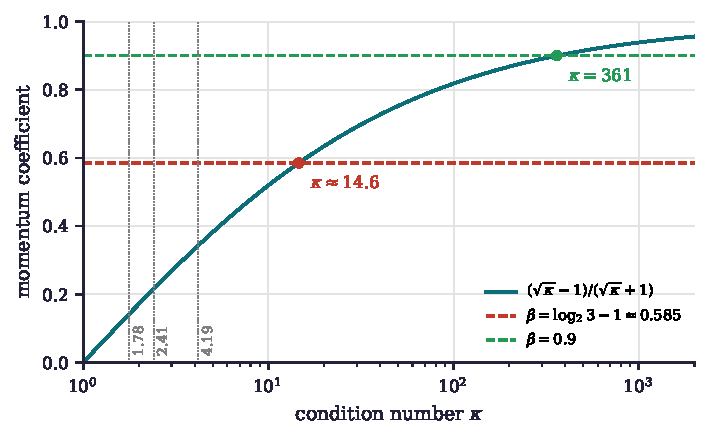
\includegraphics[width=\textwidth]{figures/ch5_nesterov_beta.pdf}
\caption{The optimal constant Nesterov coefficient
$(\sqrt\kappa-1)/(\sqrt\kappa+1)$ on $\kappa$ conditioned quadratics, with the
fixed values $\beta=\lt-1\approx0.585$ and $\beta=0.9$. The crossings, at
$\kappa=((1+\beta)/(1-\beta))^2$, are $\kappa\approx14.6$ and $\kappa=361$. Dotted
vertical lines mark the ratios $1.78$, $2.41$ and $4.19$ of
\cref{tab:ch5:levels}.}
\label{fig:ch5:nesterov}
\end{figure}

The figure states the practitioner's dilemma that opens \cref{chap:smm}: the
optimal coefficient needs $\kappa$, which is usually unknown.  The alternative
pursued there is to fix the coefficient in advance at the number
\eqref{eq:ch5:beta}, the overshoot of an injection measured in corrections.
The figure also shows the price.  The value $0.585$ is the
right amount of momentum only near $\kappa=14.6$ and is too little for harder
problems; \cref{chap:smm} shows that on quadratics the resulting method is not
accelerated at all, and \cref{chap:noise} locates its real advantage
elsewhere, in robustness to noisy gradients.  The second ingredient taken from
the arithmetic is the parity pattern: the Collatz orbit injects only on odd
steps, and Switching MM\index{Switching MM} extrapolates only on odd iterations.  In the language
of this chapter, it is a momentum method whose overshoots are always followed
by a correction, which is the one feature of the Collatz orbit that
\cref{prop:nocons} guarantees.
\Cref{chap:mmcollatz} first presses the majorization idea as far as it will go on the Collatz map itself; \cref{chap:smm,chap:noise} then develop the optimizer, exactly on quadratics and under noise; and \cref{chap:difference}, at the end of Part II, places both objects, the Collatz recursion and the momentum methods, in the common framework of nonlinear difference equations.

\section*{Notes}

The heavy ball\index{heavy ball} method is due to Polyak~\cite{polyak1964}, whose
book~\cite{polyak1987} remains the clearest treatment of momentum\index{momentum} and
Chebyshev\index{Chebyshev step sizes} methods on quadratics.  Nesterov\index{Nesterov acceleration}'s method appeared
in~\cite{nesterov1983}; the lower bounds showing its optimality among first
order methods, and the strongly convex version with constant momentum, are in
his lectures~\cite{nesterov2004}.  The failure of heavy ball to converge
globally on a strongly convex function, and a systematic method for certifying
first order algorithms by small semidefinite programs, are in Lessard, Recht
and Packard~\cite{lessard2016}.  The differential equation
\eqref{eq:ch5:sbc} is from Su, Boyd and Cand\`es~\cite{su2016}, and the high
resolution equations \eqref{eq:ch5:hrhb} and \eqref{eq:ch5:hrnag} from Shi, Du,
Jordan and Su~\cite{shi2022}; Lyapunov functions\index{Lyapunov function} for accelerated methods in
continuous and discrete time are developed systematically by Wilson, Recht and
Jordan~\cite{wilson2021}.  Restarting schemes that suppress the oscillations
of accelerated methods are studied by O'Donoghue and
Cand\`es~\cite{odonoghue2015}.

The stride constants, the per step and per macro step constants and the
identity \eqref{eq:ch5:definitional} are elementary; we present them with the
level of the iteration at which each is defined made explicit, which is the
point of \cref{rem:nesterovlimits,rem:ch5:mixing}.  \Cref{prop:ch5:nagquad} is classical; the proof given here, by
locating the double root, is the standard one.
Parrondo\index{Parrondo paradox}'s games were devised by Parrondo as a pedagogical illustration of the flashing Brownian ratchet; the capital dependent games used here were published by Harmer and Abbott~\cite{harmer1999statsci,harmer1999}, games whose rules depend on the history of play rather than on the capital were introduced by Parrondo, Harmer and Abbott~\cite{parrondo2000}, and~\cite{harmer2002} reviews both; the
observation that game B fails exactly because its residue law is not uniform
is the reason we find the analogy with Collatz parity switching useful.  For the Kullback\index{Kullback and Leibler divergence} and Leibler divergence see any text on
information theory; nothing beyond its definition is used.

\section*{Exercises}

\begin{exercise}
For the heavy ball\index{heavy ball} recursion \eqref{eq:ch5:hb} on a scalar quadratic with
curvature $\lambda$, show that the characteristic polynomial is
$z^2-(1+\beta-\alpha\lambda)z+\beta$.  With the tuning \eqref{eq:ch5:hbtune},
show that both endpoints $\lambda=\mu$ and $\lambda=L$ give double roots of
modulus $(\sqrt\kappa-1)/(\sqrt\kappa+1)$, and that every interior $\lambda$
gives complex roots of modulus $\sqrt\beta$, which is the same number.
\end{exercise}

\begin{exercise}
Verify the energy identity \eqref{eq:ch5:energy}.  For the quadratic
$f(x)=\tfrac12\lambda x^2$ and $\gamma<2\sqrt\lambda$, show that $f(X(t))$ is
not monotone even though $\mathcal E(t)$ is.  Find the analogous discrete
energy for \eqref{eq:ch5:hb} on a scalar quadratic, that is, a positive
definite quadratic form in $(x_t,x_{t-1})$ that decreases along the
iteration whenever the spectral radius is less than one.
\end{exercise}

\begin{exercise}
Compute the stride ratio and the Nesterov\index{Nesterov acceleration} style rate when $L$ is defined as
the supremum of the stride increment over odd $x\ge X$, for $X=3,7,11,\dots$,
and show that the ratio decreases to $\log(3/2)/\log(4/3)=\beta/(1-\beta)$ as
$X\to\infty$.  Explain why this dependence on $X$ is evidence that the stride
ratio is not a condition number\index{condition number}.
\end{exercise}

\begin{exercise}
Let $a,b>0$ with $a<b$ and define $\beta(a,b)=\log(1+a)/\log(1+b)$, the ascent
to descent ratio of a map that multiplies by $1+a$ on one parity class and
divides by $1+b$ on the other.  Show that
$1-\bigl(\log(1+b)-\log(1+a)\bigr)/\log(1+b)=\beta(a,b)$ identically, and
deduce that the identity \eqref{eq:ch5:definitional} holds for every map of
this type.  For which $a$ and $b$ is $\beta(a,b)$ also a ratio
$\KL(U_m\,\|\,U_{m+1})/\KL(U_n\,\|\,U_{n+1})$ of nested uniform divergences?
\end{exercise}

\begin{exercise}
For the capital dependent Parrondo\index{Parrondo paradox} game B with winning probabilities $p_0$ in
state $0$ and $p_1$ in states $1$ and $2$ (capital modulo $3$), show that the
stationary probability of state $0$ is
\[
  \pi_0=\frac{1-p_1+p_1^2}{3-p_0-2p_1+2p_0p_1+p_1^2}.
\]
Hence verify that $\pi_0=5/13$ and the gain is $0$ for $p_0=\tfrac1{10}$,
$p_1=\tfrac34$, and that the fair mixture with game A, which has $p_0=\tfrac3{10}$
and $p_1=\tfrac58$, has $\pi_0=245/709$ and gain $18/709$.
\end{exercise}

\begin{exercise}
For an odd starting value $x_0>1$ whose orbit reaches $1$ after $N$ strides,
show that the number of ascending strides ($k_j=1$) can exceed $N/2$, as it
does for $x_0=27$.  Using \cref{prop:cesaro}, find a lower bound on the
average of $k_j$ over the descending strides in terms of the fraction of
ascending strides, and evaluate it for the orbit of $27$.
\end{exercise}

\chapter{Majorization Pressed Harder}\label{chap:mmcollatz}

\Cref{chap:lyapunov} showed that the linear majorizer\index{majorization} of $\log x$ cannot certify descent.
This chapter asks what the majorization idea can do for
the Collatz map when it is pushed as far as it will go. We obtain four things.
First, the natural majorizer of a Syracuse stride is multiplicative, not
linear; summed around a cycle, its bound \emph{is} the cycle
inequality on which \cref{chap:cycles} builds, and its minorizer is the window lemma\index{window lemma} of that chapter. The
cycle half of the conjecture becomes the question of how tight this majorizer
can be made along a closed orbit, a reformulation rather than a method. Second, a potential that corrects $\log x$ by a bounded
function of residues is impossible, and the reason is a negative cycle
condition from shortest path theory: the residue graph of the map contains,
for every modulus, cycles of positive mean weight, among them the images of the cycles of $T$ on
the negative integers\index{negative cycles}. Third, any pointwise potential must assign a surplus to
integers with a run of trailing ones that grows linearly in the length of the
run. Fourth, majorizing over a whole run of ascents, a block, gives an exact
description of the dynamics, a renewal\index{renewal theory} process under the model, in which the descent of a block is decided
by a single $2$ adic valuation, and the resulting block potentials fail at a
computable fraction of odd integers that no choice of weight brings below $0.143$.
Together the failures locate the conjecture
where \cref{chap:computation} will also put it, in the integrality of $n$.

\section{The multiplicative majorizer}\label{sec:ch5c:mult}

The tangent line majorizer\index{MM algorithm} of \cref{chap:lyapunov} bounds $\log y$ by a linear function of
$y$, which is tight for $y$ near $x$ and poor at $y=3x+1$. The Syracuse map\index{Syracuse map} is
multiplicative, and the right surrogate is multiplicative too.

\begin{proposition}[Stride majorizer]\label{prop:ch5c:stride}
For odd $x\ge1$ with $k=\vt(3x+1)$,
\begin{equation}\label{eq:ch5c:stride}
\begin{gathered}
  \log S(x)=\log x+\log3-k\log2+\varepsilon(x),\\
  0<\varepsilon(x)=\log\Bigl(1+\frac1{3x}\Bigr)\le\frac1{3x},
\end{gathered}
\end{equation}
so that $g(x):=\log x+\log3-k\log2+1/(3x)$ bounds $\log S(x)$ from above,
with gap $1/(3x)-\varepsilon(x)<1/(18x^2)$, and the surrogate decrease
$\log x-g(x)=k\log2-\log3-1/(3x)$ is a lower bound for the true
decrease $\log x-\log S(x)$.
\end{proposition}

\begin{proof}
$3x+1=3x(1+1/(3x))$, and $u-u^2/2<\log(1+u)\le u$ for $u>0$.
\end{proof}

This is the surrogate bound in multiplicative form, not a descent property: the
surrogate decrease is negative whenever $k=1$, and no minimization step is
involved, so the Syracuse map is not an MM iteration in the usual sense, any
more than $T_0$ is. What the multiplicative form gains over the tangent line
bound of \cref{prop:mmdescent} is accuracy: the surrogate
decrease is exactly computable from the halving exponent, and it underestimates
the true decrease by less than $1/(18x^2)$.
The surrogate misses the true decrease only by this second order gap; what separates the map from the model decrease $k\log2-\log3$ are the terms $\varepsilon(x)\approx1/(3x)$, which the majorization\index{majorization} keeps up to that gap, and those are the entire content of the cycle half.

\begin{proposition}[The cycle inequality from the stride majorizer]\label{prop:ch5c:cyclemm}
Let $x_1,\dots,x_r$ be the odd elements of a cycle of $S$ with halving
exponents $k_1,\dots,k_r$ and $s=\sum k_i$. Summing \eqref{eq:ch5c:stride}
around the cycle gives
\[
  0=\sum_{i=1}^r\bigl(\log S(x_i)-\log x_i\bigr)
  =r\log3-s\log2+\sum_{i=1}^r\varepsilon(x_i),
\]
so $\Lambda=s\log2-r\log3=\sum_i\varepsilon(x_i)\in(0,r/(3M))$ with $M=\min_ix_i$, which is
the cycle identity that \cref{chap:cycles} proves as \cref{lem:cycleid}. The surrogate decrease around the cycle, $\Lambda-\sum
1/(3x_i)$, is negative, and the true decrease is zero: a cycle is exactly an
orbit along which the multiplicative majorizer is too pessimistic by the whole
accumulated gap.
\end{proposition}

The companion inequality is a \emph{minorization}. The affine identity of
\cref{chap:parity}, applied to the $s$ steps of $T$, $r$ of them odd, that return an element $x$ of the cycle to itself, writes $x=c_s(x)/(2^s-3^r)$, and the trivial lower
bound $c_s(x)\ge3^r-2^r$ gives the lower end of the window in the window lemma\index{window lemma} that \cref{chap:cycles} proves (\cref{lem:ch8:window}, with $m=r$ and $k=s$).
So the two halves of the window are the majorizer and
minorizer of the same quantity, the total gap $\sum\varepsilon(x_i)$, and
part (i) of \cref{cor:ch8:window} there records that an improvement of the upper end by the ratio of the two ends, a factor of about $r/3$ when $\Lambda$ is small, for every $r$ and $s$ would close the window and exclude every nontrivial cycle.

\section{Residue potentials and negative cycles}\label{sec:ch5c:residue}

For the divergence half the natural MM refinement is to correct the potential
by a function of the residue of $x$. \Cref{thm:nolyapunov} rules out monotone
potentials, but $V(x)=\log x+\varphi(x\bmod2^d)$ is not monotone, and one might
hope to choose $\varphi$ so that $V$ decreases at every step of $T$ for all
large $x$. The question has an exact answer, and it is negative for every $d$.

Fix $d$ and consider the directed graph $G_d$ on the residues modulo $2^d$ in
which $a$ has an edge to each residue $a'$ with $a'\equiv T(a)\pmod{2^{d-1}}$,
the two lifts of $T(a)$, with weight $w(a)=\log(3/2)$ if $a$ is odd and
$w(a)=-\log2$ if $a$ is even. For large $x\equiv a$ the step $x\mapsto T(x)$
changes $\log x$ by $w(a)+O(1/x)$ and moves the residue along an edge of $G_d$.

\begin{theorem}[Residue potentials]\label{thm:ch5c:residue}
\leavevmode
\begin{enumerate}[label=(\roman*),leftmargin=2em]
\item There is a function $\varphi$ on $\Z/2^d\Z$ and $X$ such that
  $V(T(x))<V(x)$ for all $x\ge X$, with $V=\log x+\varphi(x\bmod2^d)$, if and
  only if every cycle of $G_d$ has negative total weight.
\item For every $d\ge1$ the graph $G_d$ contains cycles of positive weight: the
  loop at $-1$, of weight $\log(3/2)$, and the images of the cycles of $T$ on
  the negative integers\index{negative cycles}, whose weights are $r\log3-s\log2>0$ for a cycle with
  $r$ odd steps among $s$. The maximum cycle mean of $G_d$ is exactly
  $\log(3/2)$ for every $d$.
\item Consequently no potential $\log x+\varphi(x\bmod2^d)$ with bounded
  $\varphi$ decreases at every step for all large $x$, for any $d$, and the
  same holds for potentials over any fixed number $J$ of steps.
\end{enumerate}
\end{theorem}

\begin{proof}
(i) Suppose such $\varphi$ exists and let $a_0\to a_1\to\cdots\to a_\ell=a_0$
be a cycle of $G_d$. By the theorem of Terras\index{Terras, R.} and
Everett\index{Everett, C. J.} (\cref{thm:terras}) the residue class of $x$ modulo
$2^{d+\ell}$ determines $T^i(x)\bmod2^d$ for $i\le\ell$, and the two lifts of
$x\bmod2^{d+i}$ to $2^{d+i+1}$ send $T^{i+1}(x)\bmod2^d$ to the two lifts of
$T^{i+1}(x)\bmod2^{d-1}$; so every walk of length $\ell$ in $G_d$ is realized
by a residue class modulo $2^{d+\ell}$, which contains integers $x\ge2^\ell X$, so that $T^i(x)\ge X$ for $i<\ell$. Along
the corresponding $\ell$ steps the actual increments are $w(a_i)$ plus a
positive correction at odd steps, and $\varphi$ returns to its starting value,
so $V(T^\ell(x))-V(x)\ge\sum_iw(a_i)$; strict decrease forces
$\sum_iw(a_i)<0$. Conversely, if every cycle has negative weight then, $G_d$
being finite, there is $\eta>0$ such that every cycle still has negative weight
for the shifted weights $w+\eta$. Let $\varphi(a)$ be the maximum weight, for
the shifted weights, of a walk starting at $a$ (finite because no cycle has
nonnegative shifted weight, and at least $0$ by the empty walk). Then
$\varphi(a)\ge w(a)+\eta+\varphi(a')$ for every edge $(a,a')$, so
$V(T(x))-V(x)=w(a)+\varphi(a')-\varphi(a)+O(1/x)\le-\eta+O(1/x)<0$ for $x\ge X$.

(ii) The residue $-1\bmod2^d$ is odd and $T(-1)=-1$, so $G_d$ has a loop at
$-1$ of weight $\log(3/2)$. A cycle of $T$ on negative integers with $r$ odd and
$s-r$ even steps maps to a closed walk in $G_d$ of weight
$r\log(3/2)-(s-r)\log2=r\log3-s\log2$, which is positive because $3^r>2^s$ for negative cycles: for an element $x<0$ of the
cycle the affine identity\index{cycle identity} \eqref{eq:ch2:affine} gives $(2^s-3^r)x=c_s(x)>0$. For
the maximum cycle mean, every edge weight is at most $\log(3/2)$, so no cycle
has mean above $\log(3/2)$, and the loop attains it. We also computed the
maximum cycle mean of $G_d$ by Karp's algorithm\index{Karp, R. M.} for $2\le d\le10$ and found
$\log(3/2)$ in every case (script \texttt{ch5c\_mm.py}).

(iii) is (i) and (ii), and the $J$ step version follows by applying (i) to the
graph of $J$ step walks, whose cycles are closed walks of $G_d$ and include the loop at $-1$ traversed $J$ times.
\end{proof}

\Cref{fig:ch5c:residue}(a) draws $G_5$ with three of its positive cycles, the loop at $-1$ and the images of the cycles of $T$ through $-5$ and $-17$, whose means are $0.405$, $0.039$ and $0.006$.
In all $G_5$ has $91$ simple cycles of positive weight among its $30\,176$ simple cycles (script \texttt{ch5c\_mm.py}).
By \cref{thm:terras} a closed walk in $G_d$ is determined by its parity word, and it is the trace of the periodic point of $T$ with that word; so the positive cycles are the traces of cycles of $T$ on negative rationals with odd denominator, such as $-19/11\mapsto-23/11\mapsto-29/11\mapsto-38/11$, whose trace is the cycle $7\to27\to9\to14\to7$, and the three drawn are the traces of the cycles through negative integers.
The theorem turns the obstruction that \cref{chap:computation} will describe, the point $-1$ of the exceptional set $E$ of $2$ adic integers with infinite coefficient stopping time (\cref{def:ch2:stopping}), into the language of optimization: the residue graph has a positive cycle, so no potential on residues can be a Lyapunov function\index{Lyapunov function}, exactly as a shortest path problem with a negative cycle, here for the edge lengths $-w$, has no feasible potential.
The cycles of $T$ on the negative integers are not a curiosity here; they are the simplest witnesses of why residue arithmetic cannot certify the positive integers.
A certificate\index{certificate} would have to beat the loop at $-1$ at every modulus, and the loop has mean $\log(3/2)$ whatever the modulus.

\begin{figure}[ht]
\centering
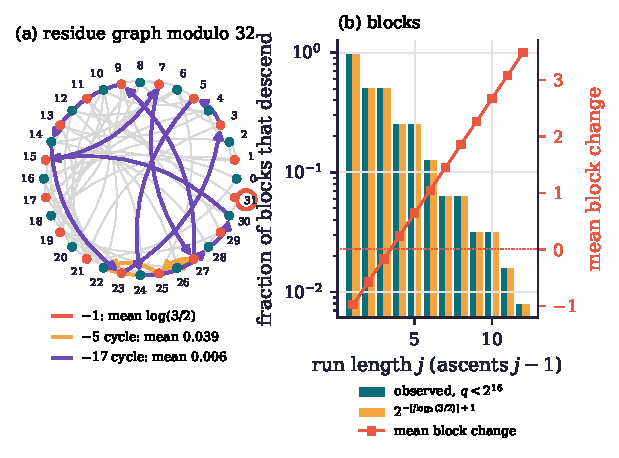
\includegraphics[width=\textwidth]{figures/ch5c_residue_blocks.pdf}
\caption{(a) The residue graph $G_5$ modulo $32$, its odd and even residues in two shades and its edges in grey, and three of its $91$ simple cycles of positive weight, the images of the cycles of $T$ on the negative integers, highlighted with their mean weights. (b) Blocks: the fraction of blocks of run length $j$ that descend, from an exact scan over $q<2^{16}$ and from the formula $2^{-\lceil j\log_2(3/2)\rceil+1}$ of \cref{prop:ch5c:block}, with the mean block change $(j-1)\log(3/2)+\log3-3\log2$ under the model.}
\label{fig:ch5c:residue}
\end{figure}

\section{What a pointwise potential must read}\label{sec:ch5c:surplus}

Residues modulo $2^d$ read $d$ bits of $x$. The chains of
\cref{prop:ch4:chain} show that the number of bits a potential must read is
unbounded, and the following proposition makes the requirement quantitative.

\begin{proposition}[Surplus along chains]\label{prop:ch5c:surplus}
Suppose $V(x)=\log x+\varphi(x)$ satisfies $V(S(x))<V(x)$ for every odd $x\ge3$.
Then for every $j\ge2$ and odd $q\ge1$,
\[
  \varphi(2^jq-1)-\varphi(2\cdot3^{j-1}q-1)\;>\;(j-1)\log\frac32 .
\]
In particular $\varphi$ is unbounded above or below, and
$\sup\varphi-\inf\varphi\ge(j-1)\log(3/2)$ for every $j$.
\end{proposition}

\begin{proof}
By \cref{prop:ch4:chain} the first $j-1$ strides from $x=2^jq-1$ are
$x_i=3^i2^{j-i}q-1$, each with $k=1$, and
$\log(x_{i+1}/x_i)=\log\bigl((3\cdot2^{j-i-1}q\cdot3^i-1)/(3^i2^{j-i}q-1)\bigr)
>\log(3/2)$, since $2(3^{i+1}2^{j-i-1}q-1)>3(3^i2^{j-i}q-1)$. Summing the
strict decreases $V(x_{i+1})<V(x_i)$ over $i=0,\dots,j-2$ gives
$\varphi(x_{j-1})-\varphi(x_0)<-\sum_i\log(x_{i+1}/x_i)<-(j-1)\log(3/2)$.
\end{proof}

So a pointwise potential must give the integer $2^jq-1$, whose binary expansion
ends in $j$ ones, a surplus of at least $(j-1)\log(3/2)$ over the integer
$2\cdot3^{j-1}q-1$ it becomes after its run of ascents. The surplus has to grow
without bound with the number of trailing ones, and trailing ones are the
simplest unbounded feature of the binary expansion. A potential that reads only
boundedly many bits cannot do this, which is \cref{thm:ch5c:residue} again; a
potential that reads the run length can, and the next section shows what
happens when it does.

\section{Block majorization}\label{sec:ch5c:block}

Let $x=2^jq-1$ with $q$ odd and $j\ge1$, so that $j-1=\vt(x+1)-1$ is the number
of ascending strides that follow. Majorize not over one stride but over the
whole \emph{block}: the $j-1$ ascents and the descent that ends them.

\begin{proposition}[Block map]\label{prop:ch5c:block}
For $x=2^jq-1$ with $q$ odd,
\begin{equation}\label{eq:ch5c:block}
  S^{(j)}(x)=\frac{3^jq-1}{2^{v}},\qquad v=\vt(3^jq-1)\ge1,
\end{equation}
and the block descends, $S^{(j)}(x)<x$, if and only if $v>j\log_2(3/2)$ (for
$x\ge3$). Under the model in which $q$ is uniform on odd residues, $v$ is
Geometric$(\tfrac12)$, the fraction of blocks of run length $j$ that descend is
$2^{-\lceil j\log_2(3/2)\rceil+1}$, and the mean change of $\log x$ over the block
is $(j-1)\log(3/2)+\log3-3\log2+O(1/x)$, which is negative for $j\le3$ and
positive for $j\ge4$.
\end{proposition}

\begin{proof}
By \cref{prop:ch4:chain}, $S^{(j-1)}(x)=2\cdot3^{j-1}q-1$, which is $\equiv1
\pmod4$; the next stride is $(3(2\cdot3^{j-1}q-1)+1)/2^k=(2\cdot3^jq-2)/2^k=
(3^jq-1)/2^{k-1}$ with $k-1=\vt(3^jq-1)$.
Comparing with $x=2^jq-1$, write $3^jq-1=2^vu$ with $u=S^{(j)}(x)$ odd; then $q(2^{j+v}-3^j)=2^v(2^jq-u)-1$, and $2^jq-u$ is odd.
If $2^{j+v}<3^j$ the left side is negative, so $u>2^jq>x$ and the block ascends.
If $2^{j+v}>3^j$ the left side is positive, so $2^jq-u$ is a positive odd integer, and $S^{(j)}(x)<x$ unless $2^jq-u=1$, that is, unless $S^{(j)}(x)=x$ and $x$ lies on a cycle consisting of a single block.
By the theorem of Steiner\index{Steiner, R. P.}~\cite{steiner1977} (see also \cite[Theorem~J]{lagarias1985}) the only such cycle is the trivial one, so for $x\ge3$ the block descends exactly when $2^{j+v}>3^j$, that is, when $v>j\log_2(3/2)$; the exact scan in \texttt{ch5c\_mm.py} agrees for every $q<2^{16}$ and $j\le12$.
For uniform odd $q$, $3^jq-1$ is uniform over
even residues, so $\Prob(v\ge i)=2^{-(i-1)}$. The threshold is the least
integer $v$ with $v>j\log_2(3/2)$, namely $\lceil j\log_2(3/2)\rceil$ when that
is not an integer, which it never is for $j\ge1$ since $\log_2(3/2)$ is
irrational; this gives the fraction. The mean change is $(j-1)\log(3/2)$ from
the ascents plus $\log3-\E[k]\log2$ with $\E[k]=\E[v]+1=3$ from the descent.
\end{proof}

The block is the natural MM unit: it is the shortest horizon over which the
surrogate can be made exact, since within a run of ascents the halving exponents
are forced to be $1$ and the only random quantity is the valuation $v$ at the
end. \Cref{fig:ch5c:residue}(b) shows the descent fractions, which the scan
reproduces exactly for $j\ge2$ (at $j=1$ it gives $1-2^{-15}$, because it includes the fixed point $x=1$), and the mean block change, which crosses zero between
$j=3$ and $j=4$. Blocks of run length four or more, that is, with three or more ascents, are, on average, net ascents.
Their rarity, $2^{-j}$ for run length $j$, is what makes the overall drift\index{drift}
negative: averaging over $j$ gives $\sum_j2^{-j}((j-1)\log(3/2)+\log3-3\log2)
=2\log(3/4)$, two strides' worth of the Syracuse drift, as it must.

\paragraph{Block potentials.} The block suggests the potential
$V_c(x)=\log x+c\,\vt(x+1)$, which pays in advance for the coming ascents.

\begin{proposition}[Run length potential]\label{prop:ch5c:runpot}
Let $V_c(x)=\log x+c\,\vt(x+1)$ with $c>\log(3/2)$. Then $V_c$ decreases at every
ascending stride from $x>1/(2(e^c-3/2))$, hence at every ascending stride when $c>\log(5/3)$ and at all but finitely many when $c\le\log(5/3)$.
The descending strides at which it fails to decrease are exactly those $x\mapsto y$, with $k$ halvings, that land on a $y$ with
$\vt(y+1)-1\ge(k\log2-\log3-\varepsilon(x))/c$. Under the model the fraction of
odd $x$ at which $V_c$ fails is
\[
  p(c)=\sum_{k\ge2}2^{-k}\,2^{-\lceil(k\log2-\log3)/c\rceil},
\]
which is $0.2087$ at $c=1$ and decreases to $0.1431$ as $c\downarrow\log(3/2)$,
and $V_c$ fails at a positive fraction of odd integers for every $c$.
\end{proposition}

\begin{proof}
At an ascending stride from $x$ with $\vt(x+1)=j\ge2$, by \eqref{eq:ch4:chain}
$\vt(S(x)+1)=j-1$ and $S(x)=(3x+1)/2$, so $V_c$ changes by $\log(3/2+1/(2x))-c$, which is negative exactly when $x>1/(2(e^c-3/2))$.
Ascending strides start at $x\ge3$, so this covers all of them when $c>\log(5/3)$; for $c\le\log(5/3)$ the stride $3\mapsto5$ fails, and for $c\le\log(11/7)$ also $7\mapsto11$ (the scan in \texttt{ch5c\_mm.py} lists the ascending failures).
At a descending stride with $k\ge2$ halvings, $\vt(x+1)=1$ and the
change is $\log3-k\log2+\varepsilon(x)+c(\vt(y+1)-1)$, which gives the stated
criterion. Under the model $k$ is Geometric$(\tfrac12)$, the descending strides being those with $k\ge2$, and $\vt(y+1)$ is an independent Geometric$(\tfrac12)$, so that $\Prob(\vt(y+1)-1\ge t)=2^{-t}$, and summing over $k$ gives $p(c)$;
the scan over odd $x<2^{20}$ gives $0.2087$ at $c=1$, matching the model to four
digits (\cref{fig:ch5c:runpot}). Positivity of $p(c)$ is clear from the $k=2$
term.
The integers fail at a positive fraction as well: if $x\equiv9\pmod{16}$ then $k=2$, $\vt(x+1)=1$ and $y=(3x+1)/4\equiv3\pmod4$, so $\vt(y+1)\ge2$ and $V_c$ changes by more than $\log(3/4)+c=c-\log(4/3)>0$, and these $x$ are one eighth of the odd integers. (For $c\le\log(3/2)$ the ascending strides, half of the odd integers, fail instead, by the first step of the proof.)
\end{proof}

\begin{figure}[ht]
\centering
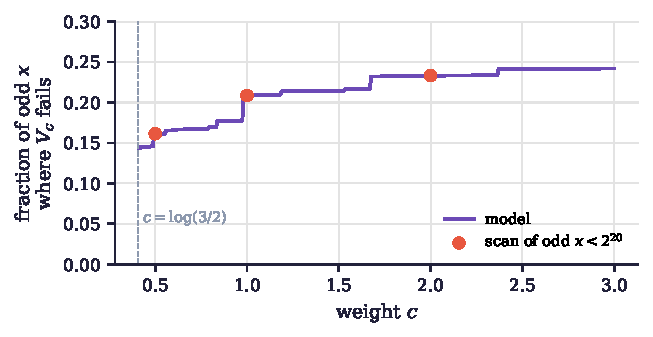
\includegraphics[width=\textwidth]{figures/ch5c_runpotential.pdf}
\caption{The fraction of odd integers at which the run length potential
$V_c=\log x+c\,\vt(x+1)$ fails to decrease over one stride, as a function of the
weight $c$: the model formula of \cref{prop:ch5c:runpot} and an exact scan of
odd $x<2^{20}$. The infimum, $0.143$, is approached as $c$ decreases to
$\log(3/2)$; below that value the ascending strides fail instead.}
\label{fig:ch5c:runpot}
\end{figure}

The run length potential does precisely what \cref{prop:ch5c:surplus} demands,
and it moves the obstruction rather than removing it. For $c>\log(5/3)$ it succeeds on every
ascent, and fails on the descents that land on an integer whose next run of
ascents is long enough to outweigh the halvings just gained. One can pay for
that run too, with a potential that reads the run after the next descent, and
then the failures move to the landing after that; the regress ends only with the
potential that reads the whole orbit to the first descent below $x$, which is
the stopping time\index{stopping time}, and whose finiteness is the conjecture. This is the
sense in which the MM approach locates the problem: each potential in this regress is
a truncation of the stopping time at some depth of the binary expansion, and
the conjecture asks, in effect, that the stopping time they truncate be finite.

\section{Majorization in expectation}\label{sec:ch5c:expectation}

There is one setting in which the majorization\index{MM algorithm} works perfectly. Under the stride model of
\cref{def:ch3:models}, take expectations in \eqref{eq:ch5c:stride}: with $k$
Geometric$(\tfrac12)$ the surrogate decrease has mean
$2\log2-\log3-1/(3x)$, which is $|\log(3/4)|$ up to $O(1/x)$, so $\log x$ is a strict supermartingale\index{martingale}\index{supermartingale} and
\cref{prop:absorb} gives absorption. Majorization in expectation is exactly the
supermartingale method, and it proves the model's version of the conjecture in
three lines. The pathwise version fails at the half of all odd integers where
$k=1$, and the preceding sections show that no repair by residues, by run
lengths, or by any bounded depth of the expansion restores it. The difference
between majorization\index{majorization} in expectation and pathwise majorization is the difference
between the model and the map, and it is the whole of the divergence half.

\section{What the approach offers}\label{sec:ch5c:verdict}

We can now state exactly what majorization\index{majorization} offers the Collatz problem.

For the cycle half it offers a reformulation: the cycle inequality is the
bound of the multiplicative majorizer summed around the cycle, the
window lemma\index{window lemma} is its minorizer, and the cycle half is the question of the
tightness of that majorizer along closed orbits. This is a clean statement and
nothing more; the arithmetic that would close the window is not supplied by
majorization.

For the divergence half it offers three impossibility results, each with a
proof: no residue potential (\cref{thm:ch5c:residue}), because the negative
cycles of $T$ are positive cycles of every residue graph; no potential $\log x+\varphi(x)$ with bounded $\varphi$
at all (\cref{prop:ch5c:surplus}); and no block potential of any weight
(\cref{prop:ch5c:runpot}). And it offers one structural fact: the block
decomposition is exact, each block's fate is
decided by the single valuation $\vt(3^jq-1)$, and under the model the blocks
form a renewal\index{renewal theory} process; the conjecture in descent
form is the statement that the sequence of blocks, started at any $n$,
reaches a block whose descent takes the orbit below $n$.

The conclusion is that majorization, pressed as hard as we are able to
press it, converts the conjecture into an equivalent termination statement with
an explicit and simple structure, and proves that the truncations of that
statement examined here, to boundedly many bits of $x$ or to a single run of
ascents, are false. What it does not do is produce the
unbounded depth argument. We believe that this is the right place to be stuck,
because, as \cref{chap:computation} will show, it is also where the automated termination provers and the $2$ adic analysis of \cref{prop:ch10b:residue}
are stuck, and three independent routes ending at the same wall is some
evidence that the wall is real.

\section*{Notes}

The negative cycle criterion for the existence of potentials is the
Bellman\index{Bellman, R.}~\cite{bellman1958} and Ford\index{Ford, L. R.}~\cite{ford1956} condition of shortest path theory, and the maximum cycle mean
is computed by Karp's algorithm\index{Karp, R. M.}~\cite{karp1978}; both are in any text on combinatorial
optimization. The observation that the negative integer cycles obstruct residue
based certificates\index{certificate} is, in the language of $2$ adic integers, the statement that $-1$, $-5$ and $-17$ lie in the exceptional set $E$ of \cref{chap:computation} (\cref{prop:ch10b:residue}); the cycles themselves are classical, see Lagarias\index{Lagarias, J. C.}~\cite{lagarias1985}.
Its formulation as a positive cycle in the residue graph, the surplus proposition and the run length potential are ours.
The block map
itself is the classical identity behind \cref{prop:ch4:chain} followed by one
descending stride; Hercher\index{Hercher, C.}~\cite[Lemma~8]{hercher2023} cites
Terras\index{Terras, R.}~\cite{terras1976} for the identity.
A cycle consisting of a single block is called a circuit, and Steiner\index{Steiner, R. P.}~\cite{steiner1977} showed that the trivial cycle is the only circuit~\cite[Theorem~J]{lagarias1985}; by the identity in the proof of \cref{prop:ch5c:block}, this is exactly the ``if'' half of the descent criterion for blocks, whose ``only if'' half is elementary.

\section*{Exercises}

\begin{exercise}
Verify by hand that the $-5$ cycle of $T$ maps to a closed walk of weight
$2\log3-3\log2$ in $G_d$ for every $d\ge2$, and locate its three residues in
$G_5$ in \cref{fig:ch5c:residue}(a).
\end{exercise}

\begin{exercise}
Show that the maximum cycle mean of $G_d$ would drop below $\log(3/2)$ if the
loop at $-1$ were deleted, compute the new maximum for $d=5$, and explain why
deleting it is not legitimate.
\end{exercise}

\begin{exercise}
Every odd $x\ge3$ is uniquely $2^jq-1$ with $q$ odd, and the block map sends it
to $S^{(j)}(x)=(3^jq-1)/2^v$. Show that under the model in which the residue of
$q$ is uniform, the pair $(j',v')$ of the next block is independent of the
current pair, with $j'$ and $v'$ independent Geometric$(\tfrac12)$, so that,
under the model, the sequence of blocks is a renewal\index{renewal theory} process. Compute the mean
number of strides per block and recover the Syracuse drift\index{drift}.
\end{exercise}

\begin{exercise}
Compute $p(c)$ of \cref{prop:ch5c:runpot} for $c=2$ and compare with the scan
value $0.2333$. Why does the failure fraction increase with $c$ for large $c$?
\end{exercise}

\begin{exercise}
Define the depth two potential $V^{(2)}_c(x)=\log x+c\,\vt(x+1)+c\,\vt(y+1)$,
where $y$ is the first element of the orbit after the next descent. Show that
it decreases at every stride except descents whose second landing has a long
run, and compute the model fraction of failures. Describe the general depth $h$
potential and its failure set.
\end{exercise}

\chapter{Switching MM}\label{chap:smm}

The previous chapters read the Collatz iteration as an optimization method:
the odd step is an injection that raises the potential $\log x$, the halvings
are the corrective descent, and \cref{chap:momentum} made precise how far the
analogy with accelerated gradient methods can be pushed before it breaks. In
this chapter and the next we run the analogy in the opposite direction. We
take two pieces of the arithmetic, a single number and a parity pattern, and
build from them an ordinary first order method for smooth optimization. The
method is called Switching MM\index{Switching MM}, abbreviated SMM. It uses the momentum\index{momentum}
coefficient
\[
  \beta \;=\; \frac{\log(3/2)}{\log 2} \;=\; \lt-1 \;\approx\; 0.585,
\]
and it applies the momentum only on odd iterations.

We want to be clear from the start about the logical status of the Collatz
material here. The arithmetic motivates the constant and the schedule; it
supplies no convergence theorem, and nothing in these two chapters bears on
the Collatz conjecture\index{Collatz conjecture}. What the arithmetic does supply is a reproducible
default that is fixed before any problem is seen. Whether that default is a
good one is a question about optimization, and we answer it with optimization
tools: an exact analysis on quadratics in this chapter, an exact noise
analysis in \cref{chap:noise}, and the experiments reported there.

This chapter rests on two results, \cref{lem:ch6:ystep} and \cref{thm:smmquad}. For every differentiable $f$, two consecutive SMM steps starting from an even index are exactly two gradient steps, of lengths $(1+\beta)\alpha$ and $\alpha$; on a quadratic the order of the two steps is immaterial, and the odd iterates lie on a cyclic gradient path as well. Switching MM is therefore a cyclic step\index{cyclic step sizes} size method in disguise, and on quadratics its behaviour can be read off from a polynomial of degree two. This reframing explains most of what the experiments of \cref{chap:noise} show, including several things that a reading of SMM as thinned momentum would not predict. \Cref{chap:difference} uses the same identity to prove that, with step $1/L$, \smmdet\ decreases $f$ on alternate iterates for every $L$ smooth $f$ and contracts the distance to the minimizer at an explicit linear rate when $f$ is also strongly convex (\cref{prop:ch5b:monotone,thm:ch5b:rate}).

\section{The practitioner's problem}\label{sec:ch6:problem}

Consider the unconstrained problem
\begin{equation}\label{eq:ch6:problem}
  \min_{x\in\R^d} f(x),
\end{equation}
where $f$ is differentiable and $L$ smooth, meaning that $\nabla f$ is
Lipschitz with constant $L$. Some of the methods we compare against also use a
strong convexity modulus $\mu>0$. Throughout we write $\alpha$ for the base step
size, usually $\alpha=1/L$.

Momentum methods add to the gradient step a multiple of the previous
displacement. Polyak\index{Polyak, B. T.}'s heavy ball\index{heavy ball} method~\cite{polyak1964} reads
\begin{equation}\label{eq:ch6:hb}
  x_{t+1} = x_t - \alpha\nabla f(x_t) + \beta(x_t-x_{t-1}),
\end{equation}
and Nesterov\index{Nesterov, Yu.}\index{Nesterov acceleration}'s accelerated gradient method~\cite{nesterov1983}, in the
constant momentum\index{momentum} form we shall use, reads
\begin{equation}\label{eq:ch6:nag}
  y_t = x_t + \beta(x_t-x_{t-1}),\qquad x_{t+1} = y_t - \alpha\nabla f(y_t).
\end{equation}
The difference is only where the gradient is evaluated. On a $\mu$ strongly
convex, $L$ smooth function with condition number\index{condition number} $\kappa=L/\mu$, the classical
tunings choose $\beta$ from $\kappa$: for Nesterov's method with $\alpha=1/L$
the textbook choice is
\begin{equation}\label{eq:ch6:betaopt}
  \beta^{\mathrm{opt}}(\kappa) = \frac{\sqrt\kappa-1}{\sqrt\kappa+1},
\end{equation}
and heavy ball uses the square of this ratio together with a modified step
$4/(\sqrt L+\sqrt\mu)^2$~\cite{polyak1987}.
On quadratics these tunings deliver the accelerated iteration count of order $\sqrt\kappa\log(1/\varepsilon)$ instead of the order $\kappa\log(1/\varepsilon)$ of gradient descent.
For Nesterov's method the same order holds on every $\mu$ strongly convex, $L$ smooth function~\cite{nesterov2004}; for heavy ball it does not, since Lessard\index{Lessard, L.}, Recht\index{Recht, B.} and Packard\index{Packard, A.}~\cite{lessard2016} give a strongly convex function on which the tuned method settles into a limit cycle (\cref{sec:ch5:momentum}).

The difficulty is that \eqref{eq:ch6:betaopt} moves with the instance. A
practitioner who solves a family of related problems, say a sequence of
regularized regressions along a path of penalty parameters, or the same model
refitted as data arrive, faces two unattractive options.
\begin{enumerate}[leftmargin=2em]
  \item \emph{Retune per instance.} Estimate $\mu$ each time and set $\beta$ by
  \eqref{eq:ch6:betaopt}. This buys near optimal speed, but estimating the
  smallest eigenvalue of a Hessian is often as expensive as the optimization
  itself, and a poor estimate can make matters worse than no momentum at all.
  \item \emph{Use the default.} Set $\beta=0.9$, the value that has become
  conventional in machine learning, for instance as the first moment
  coefficient of Adam~\cite{kingma2015}. This avoids tuning, but a high fixed
  momentum overshoots on well conditioned problems and, as
  \cref{chap:noise} shows in detail, amplifies gradient noise by a factor
  $1/(1-\beta)=10$ in the slow directions.
\end{enumerate}
The approach of this chapter is a third option: \emph{fix the momentum coefficient in advance by a rule} that uses no information about the instance, and then study what the resulting method does and does not achieve.

\section{Fixing the coefficient in advance}\label{sec:ch6:beta}

We give two derivations of the same number. Neither uses $\mu$, $\kappa$, the dimension, or any property of $f$, which is the point; both rest on the two logarithms $\log2$ and $\log(3/2)$.

\subsection{The Collatz derivation}

Recall from \cref{chap:parity} the accelerated map\index{accelerated map} $T(n)=n/2$ for even $n$ and
$T(n)=(3n+1)/2$ for odd $n$. On the logarithmic scale its increments take two
kinds of value,
\[
  \log T(n)-\log n=
  \begin{cases}
    -\log 2, & n\ \text{even},\\[2pt]
    \log\bigl(\tfrac32+\tfrac1{2n}\bigr)\in(0,\log 2), & n\ \text{odd},\ n\ge3,
  \end{cases}
\]
so every halving lowers the potential by exactly $\log 2$ while every odd step
raises it by slightly more than $\log(3/2)$. Grouping an odd step with the run
of halvings that follows it gives the Syracuse map\index{Syracuse map} $S(n)=(3n+1)/2^{k}$ with
$k=\vt(3n+1)\ge1$, and the increment of the potential across this macro step
obeys an exact identity.

\begin{lemma}[Log displacement identity]\label{lem:ch6:logdisp}
For every odd $n\ge1$, with $k=\vt(3n+1)$,
\begin{equation}\label{eq:ch6:logdisp}
  \log S(n)-\log n \;=\; \log 3 - k\log 2 + \varepsilon_n,
  \qquad \varepsilon_n=\log\Bigl(1+\frac1{3n}\Bigr),
\end{equation}
and $0<\varepsilon_n\le\log(4/3)$, with equality on the right only at $n=1$.
Moreover $\varepsilon_n<1/(3n)$, so $\varepsilon_n\to0$.
\end{lemma}

\begin{proof}
Write $3n+1=3n(1+1/(3n))$, take logarithms and subtract $k\log2$; this is
\eqref{eq:ch6:logdisp}. The function $n\mapsto\log(1+1/(3n))$ is positive and
strictly decreasing on $n\ge1$, so its maximum over odd $n$ is attained at $n=1$,
where it equals $\log(4/3)$. The bound $\log(1+u)<u$ for $u>0$ gives the last
statement.
\end{proof}

The identity separates the macro step into a fixed ascent $\log 3$, a variable
descent $k\log 2$, and a vanishing correction. In the accelerated map the ascent
is split as $\log 3=\log(3/2)+\log 2$: one halving is absorbed into the odd
step itself, and the net ascent of the odd step tends to $\log(3/2)$ as
$n\to\infty$. The asymptotic ratio of the magnitude of one ascent to the
magnitude of one descent is therefore
\begin{equation}\label{eq:ch6:betadef}
  \beta \;=\; \frac{\log(3/2)}{\log 2} \;=\; \lt-1 \;=\; 0.584963\ldots
\end{equation}
This is the number that parameterizes the two primitive moves of the parity
switching rule, and it depends on nothing else. In the language of
\cref{chap:momentum}, the odd step is the injection that overshoots and the
halving is the correction, and $\beta$ is the size of the overshoot measured in
units of the correction. Under the Geometric$(\tfrac12)$ law of \cref{prop:geom}
the mean macro step increment is $\log 3-2\log 2=\log(3/4)<0$, so the corrections
win on average; the identity $\log(3/4)=(\beta-1)\log 2$ expresses this as the
statement $\beta<1$.

\subsection{The Kullback and Leibler derivation}

The second derivation comes from elementary information theory. Let
$A_1\subset A_2\subset A_3$ be nested sets with $|A_j|=j$, and let $U_j$ be the
uniform distribution on $A_j$, viewed as a distribution on $A_3$.

\begin{lemma}[A ratio of divergences]\label{lem:ch6:kl}
$\KL(U_1\,\|\,U_2)=\log 2$ and $\KL(U_2\,\|\,U_3)=\log(3/2)$. Consequently
\begin{equation}\label{eq:ch6:betakl}
  \beta \;=\; \frac{\KL(U_2\,\|\,U_3)}{\KL(U_1\,\|\,U_2)}.
\end{equation}
\end{lemma}

\begin{proof}
Since $U_j$ is supported inside the support of $U_{j+1}$, we have
$\KL(U_j\,\|\,U_{j+1})=\sum_{a\in A_j}\tfrac1j\log\bigl(\tfrac{1/j}{1/(j+1)}\bigr)
=\log\tfrac{j+1}{j}$. Take $j=1$ and $j=2$.
\end{proof}

A divergence $\KL(P\,\|\,Q)$ is the exponential rate at which an empirical
distribution drawn from $Q$ comes to look like $P$, by Sanov\index{Sanov, I. N.}'s theorem. Read
this way, $\beta$ is the ratio of the information rates of two elementary
compressions, from three equally likely states to two and from two to one.
We invoke no specific large deviation\index{large deviations} bound and no result below depends on
this reading.
We include it because it shows the same number from another side, not as independent evidence that the constant is natural: every ratio $\log\frac{m+1}{m}\big/\log\frac{n+1}{n}$ is a ratio of divergences of nested uniform laws, and, as \cref{sec:ch5:beta} explains, the integers $2$ and $3$ do all the work in both derivations, so their agreement is forced.

\subsection{What the derivations do not show}

Two remarks guard against reading more into the derivations than is there.

\begin{remark}[A definitional identity]\label{rem:ch6:definitional}
Put $L_\ast=\log2$, the size of one halving and also the largest one step ascent of the potential under the accelerated map (attained only at $n=1$), and $\mu_\ast=|\log(3/4)|$, the mean descent per macro step under the Geometric$(\tfrac12)$ law.
Then
\[
  \beta=\frac{L_\ast-\mu_\ast}{L_\ast}=1-\frac{\mu_\ast}{L_\ast},
\]
which looks like the familiar expression of a momentum\index{momentum} coefficient in terms of
a condition number\index{condition number}. It is not a discovery: it follows at once from
$\log(3/4)=\log3-2\log2$ and the definition \eqref{eq:ch6:betadef}. The ratio
$\kappa_\ast=L_\ast/\mu_\ast=2.409$ is not a condition number: it compares a
per step extremal quantity with a per macro step expectation, and both are
increments of the potential, not curvature bounds, as \cref{rem:nesterovlimits}
explains for the closely related stride constants of \cref{def:nesterov}. No
rate follows from it. The coincidence that $1/(1-\beta)=\kappa_\ast$ will
reappear in \cref{chap:noise} as the noise amplification of every step
momentum at this $\beta$; it is the same algebra, not new evidence.
\end{remark}

\begin{remark}[Structure is not optimality]\label{rem:ch6:notoptimal}
A structural derivation makes a default reproducible and removes one tuning
decision. It does not make the default optimal for any particular problem. By
\eqref{eq:ch6:betaopt}, the value $0.585$ is the optimal Nesterov coefficient
only at $\kappa=\bigl((1+\beta)/(1-\beta)\bigr)^2=14.58$; it is too small for
more ill conditioned problems and too large for better conditioned ones.
\end{remark}

\section{The algorithm}\label{sec:ch6:alg}

The second ingredient taken from the arithmetic is the parity pattern.
Under the standard map\index{standard map} an odd step is always followed by a halving (\cref{prop:nocons}), so an injection is never followed directly by another injection, although it may be followed by several corrections.
Switching MM\index{Switching MM} imposes the simplest pattern with this property, strict alternation, which in an orbit is a run of strides with $k=1$, and it does so with the iteration counter: on odd iterations it extrapolates by $\beta(x_t-x_{t-1})$ and takes a gradient step from the extrapolated point, exactly as in \eqref{eq:ch6:nag}; on even iterations it takes a plain gradient step.
\Cref{alg:smmdet} is the formal method, which we denote \smmdet.

\begin{algorithm}[t]
\caption{\smmdet: Switching MM with deterministic parity injection}
\label{alg:smmdet}
\begin{algorithmic}[1]
\Require $\nabla f$, step size $\alpha=1/L$, initial point $x_0\in\R^d$,
horizon $T$; fixed momentum $\beta=\log(3/2)/\log 2$
\State $x_{-1}\gets x_0$
\For{$t=0,1,\dots,T-1$}
  \If{$t$ is odd}
    \State $y_t\gets x_t+\beta(x_t-x_{t-1})$ \Comment{injection: extrapolate}
    \State $x_{t+1}\gets y_t-\alpha\nabla f(y_t)$
  \Else
    \State $x_{t+1}\gets x_t-\alpha\nabla f(x_t)$ \Comment{descent: plain gradient step}
  \EndIf
\EndFor
\State \Return $x_T$
\end{algorithmic}
\end{algorithm}

We also consider an adaptive variant, \smmstate\ (\cref{alg:smmstate}), which injects momentum\index{momentum} only when the most recent reduction of a merit gap was inadequate. It needs two extra inputs, a reference value $f_{\mathrm{ref}}\le\inf f$ and a threshold $\rho_{\mathrm{thr}}\in(0,1)$. We take $\rho_{\mathrm{thr}}=0.356$, which is $1-\kappa_\ast^{-1/2}$ for the ratio $\kappa_\ast=2.409$ of \cref{rem:ch6:definitional}, the number in the rate column of \cref{tab:ch5:levels}; it is carried over from the Collatz constants untuned, and like that column it has no theorem behind it. We report \smmstate\ as an empirical probe only; the one result that covers it is the analysis of arbitrary switching on quadratics in \cref{chap:difference}, where \cref{cor:ch5b:anyswitch} proves, conditionally on \cref{conj:ch5b:transient}, that every switching rule is stable. The claim that SMM has no tuned momentum coefficient attaches to \smmdet, and all the theory below concerns \smmdet.

\begin{algorithm}[t]
\caption{\smmstate: adaptive injection variant}
\label{alg:smmstate}
\begin{algorithmic}[1]
\Require $f$, $\nabla f$, $\alpha=1/L$, $x_0$, $T$, reference value
$f_{\mathrm{ref}}\le\inf f$, threshold $\rho_{\mathrm{thr}}\in(0,1)$, small
$\epsilon>0$; $\beta=\log(3/2)/\log 2$
\State $x_{-1}\gets x_0$; \quad $g_{\mathrm{prev}}\gets\max(f(x_0)-f_{\mathrm{ref}},\epsilon)$
\For{$t=0,1,\dots,T-1$}
  \State $g_t\gets\max(f(x_t)-f_{\mathrm{ref}},\epsilon)$ \Comment{nonnegative merit gap}
  \If{$t=0$ \textit{or} $g_t/g_{\mathrm{prev}}>\rho_{\mathrm{thr}}$}
    \State $y_t\gets x_t+\beta(x_t-x_{t-1})$; \quad $x_{t+1}\gets y_t-\alpha\nabla f(y_t)$
    \Comment{progress too slow: inject}
  \Else
    \State $x_{t+1}\gets x_t-\alpha\nabla f(x_t)$ \Comment{progress adequate: descend}
  \EndIf
  \State $g_{\mathrm{prev}}\gets g_t$
\EndFor
\State \Return $x_T$
\end{algorithmic}
\end{algorithm}

\subsection{Relation to heavy ball and Nesterov}

The injection step of \smmdet\ is the Nesterov\index{Nesterov acceleration} update \eqref{eq:ch6:nag} with
fixed momentum\index{momentum} $\beta$, and the descent step is gradient descent. Equivalently,
\smmdet\ is fixed momentum Nesterov at $\beta=0.585$ with the extrapolation
switched off on every other iteration. Heavy ball \eqref{eq:ch6:hb} injects at
every iteration and evaluates the gradient before extrapolating; when we speak
of every step momentum we mean either of \eqref{eq:ch6:hb} and
\eqref{eq:ch6:nag} applied at every iteration with the same fixed $\beta$.

The restriction to injection on alternate steps is unusual. Every classical
inertial method injects at every step, and \cref{sec:ch6:cyclic} shows that in
the noiseless setting the restriction costs a constant factor in speed. The
reason for keeping it is the noise analysis of \cref{chap:noise}: alternation
caps the amplification of gradient noise uniformly in $\beta$.

\Cref{fig:ch6:traj} shows the mechanism on a tilted two dimensional quadratic
with $\kappa=8$. The injection steps of \smmdet\ push the iterate along the
valley floor, and the objective decreases faster than under gradient descent.
After $28$ steps from $x_0=(1.3,0.9)$ the objective is $8.5\times10^{-5}$ under
gradient descent and $7.4\times10^{-6}$ under \smmdet. The adaptive rule of
\smmstate\ fires on $24$ of the $28$ steps on this instance, because the
progress per step along the slow direction rarely beats the threshold
$\rho_{\mathrm{thr}}$, and it behaves almost like every step Nesterov: it ends
at $7.3\times10^{-10}$, against $2.2\times10^{-9}$ for every step Nesterov at the
same $\beta$ (script \texttt{ch6\_trajectory.py}). In the noiseless setting
more injection is better; \cref{chap:noise} explains why the conclusion
reverses under noise.

\begin{figure}[t]
  \centering
  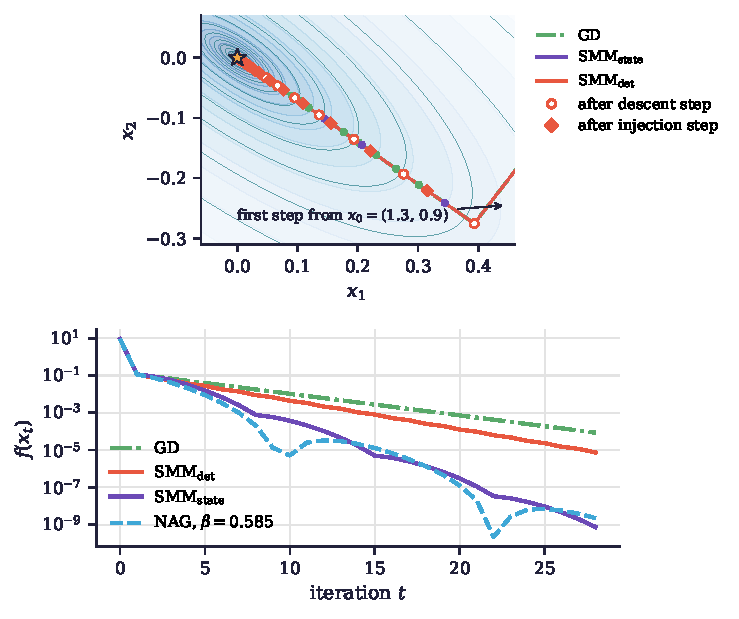
\includegraphics[width=\textwidth]{figures/ch6_trajectory.pdf}
  \caption{\smmdet\ on a tilted two dimensional quadratic with $\kappa=8$ and
  step $1/L$. Top: contours and the first iterates of gradient descent,
  \smmdet\ and \smmstate; open circles mark the points reached after descent
  steps and filled diamonds those after injection steps. Bottom: objective value
  on a log scale over $28$ iterations, with every step Nesterov at the same
  $\beta$ for comparison.}
  \label{fig:ch6:traj}
\end{figure}

\subsection{What the method needs}

\smmdet\ requires the smoothness constant $L$, for the step size, and nothing
else. Heavy ball and Nesterov\index{Nesterov acceleration} in their textbook strongly convex tunings need
both $L$ and $\mu$. The fixed momentum\index{momentum} baselines of \cref{chap:noise} need $L$
and a chosen $\beta$, and the point of the structural derivation is that SMM
does not leave that choice to the user. Memory cost is one extra vector, the
previous iterate, the same as for heavy ball\index{heavy ball} and Nesterov and less than for
adaptive methods such as Adam, which keep two moment vectors.

\section{Candidate fixed momenta}\label{sec:ch6:candidates}

The value $0.585$ is one of several natural fixed coefficients.
\Cref{tab:ch6:candidates} lists the four that the experiments of
\cref{chap:noise} compare, with the condition number\index{condition number} at which each would be the
optimal Nesterov\index{Nesterov acceleration} coefficient \eqref{eq:ch6:betaopt}, namely
$\kappa=\bigl((1+\beta)/(1-\beta)\bigr)^2$, and the slow mode noise amplification
$1/(1-\beta)$ of every step momentum\index{momentum} derived in \cref{chap:noise}.

\begin{table}[t]
\centering
\caption{Candidate fixed momentum coefficients. The column $\kappa$ gives the
condition number at which $\beta$ equals the optimal Nesterov coefficient; the
last column is the slow mode variance amplification of every step momentum
relative to gradient descent.}
\label{tab:ch6:candidates}
\small\setlength{\tabcolsep}{4pt}
\begin{tabular}{llcc}
\toprule
$\beta$ & Origin & $\kappa$ where optimal & $1/(1-\beta)$\\
\midrule
$0.500$ & round number & $9.0$ & $2.00$\\
$0.585$ & $\log_2(3/2)$, Collatz and KL ratio & $14.6$ & $2.41$\\
$0.667$ & $2/3$ & $25.0$ & $3.00$\\
$0.900$ & machine learning default~\cite{kingma2015} & $361$ & $10.0$\\
\bottomrule
\end{tabular}
\end{table}

None of these is uniformly best, and the experiments confirm it: $0.585$ does
well at small $\kappa$, $0.667$ is best on a mildly ill conditioned logistic
regression, and $0.9$ wins on strongly ill conditioned quadratics.
What distinguishes $0.585$ is not performance but provenance: it is the only entry that the arithmetic of the Collatz map fixes, rather than a round number or a convention.

\section{Related work}\label{sec:ch6:related}

\paragraph{Fixed momentum methods.} SMM belongs to the tradition of inertial
first order methods that runs from Polyak's heavy ball\index{heavy ball}~\cite{polyak1964} through
Nesterov\index{Nesterov acceleration}'s accelerated gradient~\cite{nesterov1983}; Polyak's
monograph~\cite{polyak1987} remains the clearest source for their analysis on
quadratics. The ordinary differential equation view of
Su\index{Su, W.}, Boyd\index{Boyd, S.} and Cand\`es\index{Candes, E. J.@Cand\`es, E. J.}~\cite{su2016} and the high resolution refinement of
Shi\index{Shi, B.}, Du\index{Du, S. S.}, Jordan\index{Jordan, M. I.} and Su~\cite{shi2022} explain acceleration as the interplay of
an inertial term and a gradient correction.
That picture describes every step momentum with $\beta$ tending to $1$ as the step shrinks. SMM has no inertial limit: whatever the value of $\beta<1$, its continuous time limit is a first order gradient flow, because two of its steps are two gradient steps (\cref{lem:ch6:ystep}) and it carries one gradient of memory rather than a velocity (\cref{prop:ch5b:modified}).

\paragraph{Low tuning design.} A recurring theme in modern optimization is the
search for methods whose defaults work across instances. Iterate averaging in
stochastic approximation~\cite{ruppert1988,polyak1990,polyak1992} and adaptive moment methods such as
Adam~\cite{kingma2015} are two successful examples. SMM is adjacent in spirit,
but takes its fixed coefficient from a structural source instead of from an
adaptive estimate.

\paragraph{Arithmetic structure in optimization.} Number theoretic structure
enters optimization in several established ways. Fibonacci search, which
Kiefer\index{Kiefer, J.}~\cite{kiefer1953} proved minimax optimal for unimodal functions, uses
ratios of Fibonacci numbers, and in the limit the golden ratio, to place
function evaluations. Quasi Monte Carlo methods~\cite{niederreiter1992} use
low discrepancy sequences and lattice rules built from modular arithmetic to
derandomize integration and stochastic optimization. In both cases arithmetic
decides \emph{where to evaluate}. SMM differs in where the arithmetic enters:
it decides \emph{how much inertial memory to retain}, and when.

\paragraph{Switching systems.} Alternating between two linear updates is a
switched linear system, and the stability of such systems under arbitrary or
periodic switching is the subject of Liberzon\index{Liberzon, D.}'s monograph~\cite{liberzon2003}.
Periodic switching is the benign case: stability is decided by the spectral
radius of the product of the matrices over one period, and
\cref{sec:ch6:cyclic} computes that product in closed form.

\paragraph{Majorization and minimization.} The descent half of SMM is a
majorization\index{majorization} minimization step in the sense of Lange\index{Lange, K.}, Hunter\index{Hunter, D. R.} and
Yang\index{Yang, I.}~\cite{lange2000} and Hunter and Lange~\cite{hunter2004}: for $L$ smooth
$f$ the gradient step minimizes the quadratic upper bound
$f(x_t)+\nabla f(x_t)^\top(x-x_t)+\tfrac L2\|x-x_t\|^2$. Mairal\index{Mairal, J.}~\cite{mairal2015}
develops incremental versions of this principle for large scale learning.
At the level of the optimizer the MM reading supplies the descent inequality behind \cref{prop:ch5b:monotone}: \smmdet\ is the momentum MM scheme of \cref{sec:ch5b:mm}, with the majorization point extrapolated on odd iterations.
In the Collatz
setting of \cref{chap:lyapunov} the tangent line of $\log x$ bounds the increment
of the potential at every step of $T_0$, but the map is not an MM iteration in
the usual sense, and \cref{prop:mmfails} shows that the bound cannot certify
descent. That reading of the Collatz map is the origin of the name Switching
MM\index{Switching MM}.

\paragraph{Step size schedules.} The connection that turns out to matter most
is invisible in the momentum reading of the method.
Varying the step size
periodically in gradient descent on quadratics goes back to
Richardson\index{Richardson, L. F.}~\cite{richardson1911}; Young\index{Young, D.}~\cite{young1953} showed how to choose
the steps from the roots of Chebyshev\index{Chebyshev step sizes} polynomials, and Golub\index{Golub, G. H.} and
Varga\index{Varga, R. S.}~\cite{golub1961} connected these schedules to second order iterations of
heavy ball type. Much more recently Altschuler\index{Altschuler, J. M.} and Parrilo\index{Parrilo, P. A.}~\cite{altschuler2024}
showed that carefully designed nonconstant step size schedules, the silver
stepsize schedule, accelerate gradient descent on smooth convex problems beyond
what any constant step achieves. \Cref{thm:smmquad} places SMM in this family.

\section{Switching MM is a cyclic step size method}\label{sec:ch6:cyclic}

We now analyse \smmdet\ exactly. Write $G_h(x)=x-h\nabla f(x)$ for a gradient step
of length $h$. The starting observation is an identity valid for every
differentiable $f$.

\begin{lemma}[The extrapolated point is a long gradient step]\label{lem:ch6:ystep}
Let $t$ be even. Then $x_{t+1}=G_\alpha(x_t)$, and the extrapolated point at
the following odd iteration is
\begin{equation}\label{eq:ch6:ystep}
  y_{t+1} = x_{t+1}+\beta(x_{t+1}-x_t) = x_t-(1+\beta)\alpha\nabla f(x_t)
  = G_{(1+\beta)\alpha}(x_t).
\end{equation}
Consequently $x_{t+2}=G_\alpha\bigl(G_{(1+\beta)\alpha}(x_t)\bigr)$, and in the
form that exhibits the momentum\index{momentum},
\begin{equation}\label{eq:ch6:general}
  x_{t+2} = x_{t+1}-\beta\alpha\nabla f(x_t)-\alpha\nabla f(y_{t+1}).
\end{equation}
\end{lemma}

\begin{proof}
At the even iteration $t$ the update is a plain gradient step, so
$x_{t+1}-x_t=-\alpha\nabla f(x_t)$. Substituting this displacement into the
extrapolation gives $y_{t+1}=x_{t+1}-\beta\alpha\nabla f(x_t)
=x_t-(1+\beta)\alpha\nabla f(x_t)$. The odd update is
$x_{t+2}=y_{t+1}-\alpha\nabla f(y_{t+1})$, which gives both displayed forms.
\end{proof}

So the even iterates $x_0,x_2,x_4,\dots$ of \smmdet\ are \emph{exactly} every second iterate of gradient descent with the periodic step sizes $(1+\beta)\alpha,\alpha,(1+\beta)\alpha,\alpha,\dots$, whose intermediate iterates are the extrapolated points $y_{t+1}$, for any $f$.
The momentum
buffer of \smmdet\ never holds anything except the last gradient, so the
extrapolation simply lengthens that gradient step by the factor $1+\beta$. The
odd iterates $x_{t+1}$ are an observation point off this path. On a quadratic
they lie on a second cyclic path, because gradient steps commute.

\begin{theorem}[Two step equivalence on quadratics]\label{thm:smmquad}
Let $f(x)=\tfrac12x^\top Ax-b^\top x$ with $A$ symmetric positive definite and
minimizer $x^\ast=A^{-1}b$, let $\alpha>0$ and $\beta\ge0$, and let $(x_t)$ be
generated by \cref{alg:smmdet} with step $\alpha$. For every even $t\ge0$,
\begin{equation}\label{eq:ch6:twostep}
  x_{t+2} = G_{(1+\beta)\alpha}(x_{t+1}) = G_{(1+\beta)\alpha}\bigl(G_\alpha(x_t)\bigr),
\end{equation}
that is, two \smmdet\ steps from an even index are a gradient step of length
$\alpha$ followed by a gradient step of length $(1+\beta)\alpha$, and every
iterate of \smmdet\ is an iterate of this cyclic schedule. In terms of the
error $e_t=x_t-x^\ast$,
\begin{equation}\label{eq:ch6:twosteperr}
  e_{t+2} = (I-\alpha A)\bigl(I-(1+\beta)\alpha A\bigr)e_t,\qquad t\ \text{even}.
\end{equation}
\end{theorem}

\begin{proof}
For a quadratic, $\nabla f(x)=A(x-x^\ast)$, so a gradient step of any length $h$
acts on the error linearly: $G_h(x)-x^\ast=(I-hA)(x-x^\ast)$. By
\cref{lem:ch6:ystep}, for even $t$,
\begin{gather*}
  e_{t+1}=(I-\alpha A)e_t,\qquad
  y_{t+1}-x^\ast=\bigl(I-(1+\beta)\alpha A\bigr)e_t,\\
  e_{t+2}=(I-\alpha A)(y_{t+1}-x^\ast),
\end{gather*}
and therefore $e_{t+2}=(I-\alpha A)(I-(1+\beta)\alpha A)e_t$, which is
\eqref{eq:ch6:twosteperr}. The matrices $I-\alpha A$ and $I-(1+\beta)\alpha A$
are both polynomials in $A$, hence commute, so also
\[
  e_{t+2}=\bigl(I-(1+\beta)\alpha A\bigr)(I-\alpha A)e_t
  =\bigl(I-(1+\beta)\alpha A\bigr)e_{t+1},
\]
which says $x_{t+2}=G_{(1+\beta)\alpha}(x_{t+1})$. Combined with
$x_{t+1}=G_\alpha(x_t)$ this is \eqref{eq:ch6:twostep}. By induction on even
$t$, starting from $x_0$, every iterate of \smmdet\ is an iterate of gradient
descent with steps $\alpha,(1+\beta)\alpha,\alpha,(1+\beta)\alpha,\dots$.
\end{proof}

The same fact can be seen through the state space description that
the switching systems literature would use. Restricted to an eigenvector of $A$
with eigenvalue $\lambda$, and writing $a=\alpha\lambda$, the state
$(e_t,e_{t-1})$ evolves by the descent matrix $D$ on even steps and the
Nesterov\index{Nesterov acceleration} matrix $N$ on odd steps, where
\[
  D=\begin{pmatrix}1-a&0\\1&0\end{pmatrix},\qquad
  N=\begin{pmatrix}(1-a)(1+\beta)&-(1-a)\beta\\1&0\end{pmatrix}.
\]
The product over one period is
\[
  ND=\begin{pmatrix}(1-a)(1-(1+\beta)a)&0\\1-a&0\end{pmatrix},
\]
a matrix of rank one with eigenvalues $0$ and $(1-a)(1-(1+\beta)a)$. The zero
eigenvalue records that the descent step forgets $e_{t-1}$, which is why the
period map involves only $e_t$.

\subsection{Consequences}

Write
\begin{equation}\label{eq:ch6:rho}
  \rho(a)=(1-a)\bigl(1-(1+\beta)a\bigr)=1-(2+\beta)a+(1+\beta)a^2
\end{equation}
for the two step multiplier on an eigendirection with $a=\alpha\lambda$.

\begin{corollary}[Two step contraction]\label{cor:ch6:contraction}
Under the hypotheses of \cref{thm:smmquad}, for even $t$,
\[
  \|e_{t+2}\|\le\max_{\lambda\in\operatorname{spec}(A)}|\rho(\alpha\lambda)|\;\|e_t\|,
\]
with equality for a suitable $e_t$. The per step contraction factor on an
eigendirection is $|\rho(a)|^{1/2}$.
\end{corollary}

\begin{proof}
The matrix in \eqref{eq:ch6:twosteperr} is symmetric with eigenvalues
$\rho(\alpha\lambda)$, so its operator norm is the largest of their absolute
values, attained on the corresponding eigenvector.
\end{proof}

\begin{corollary}[Stability]\label{cor:ch6:stability}
Let $0\le\beta<1$. Then $|\rho(a)|<1$ if and only if
$0<a<(2+\beta)/(1+\beta)$. In particular \smmdet\ converges linearly on every
strongly convex quadratic whenever $\alpha\le1/L$, and in fact whenever
$\alpha L<(2+\beta)/(1+\beta)$. For all $a>0$,
$\rho(a)\ge1-(2+\beta)^2/(4(1+\beta))$, a minimum attained at
$a=(2+\beta)/(2(1+\beta))$.
\end{corollary}

\begin{proof}
From \eqref{eq:ch6:rho}, $\rho(a)<1$ if and only if $a\bigl((1+\beta)a-(2+\beta)\bigr)<0$,
that is $0<a<(2+\beta)/(1+\beta)$. The condition $\rho(a)>-1$ reads
$(1+\beta)a^2-(2+\beta)a+2>0$; the discriminant of this quadratic in $a$ is
$(2+\beta)^2-8(1+\beta)=\beta^2-4\beta-4$, which is negative for $0\le\beta<1$,
so the inequality holds for every $a$. The minimum of the convex quadratic
$\rho$ is at its vertex.
\end{proof}

At $\beta=\lt-1$ the stability limit is $(2+\beta)/(1+\beta)=1+\log_3 2=1.631$
and the minimum of $\rho$ is $-0.054$, attained at $a=0.815$. The multiplier
vanishes at $a=1/(1+\beta)=0.631$ and at $a=1$: those eigendirections are
annihilated in one period.

\begin{corollary}[Slow modes]\label{cor:ch6:slow}
As $a\to0$, $\rho(a)=1-(2+\beta)a+O(a^2)$, and the per step contraction factor
is $1-\tfrac{2+\beta}{2}a+O(a^2)$. Thus in the slow directions \smmdet\ behaves
like gradient descent with the effective step
\[
  m_{\mathrm{SMM}}\,\alpha,\qquad m_{\mathrm{SMM}}=\frac{2+\beta}{2}=1.2925
  \quad\text{at }\beta=\lt-1.
\]
\end{corollary}

\begin{proof}
Expand \eqref{eq:ch6:rho} and take the square root.
\end{proof}

The effective step is just the average of the two step lengths $\alpha$ and
$(1+\beta)\alpha$, as it must be for a cyclic schedule in the slow modes. For
comparison, every step momentum\index{momentum} at fixed $\beta$, heavy ball\index{heavy ball} or Nesterov\index{Nesterov acceleration}, has
in the overdamped slow regime a real dominant root $1-a/(1-\beta)+O(a^2)$, so its
effective step multiplier is
\[
  m_{\mathrm{HB}}=m_{\mathrm{NAG}}=\frac1{1-\beta}=2.409\quad\text{at }\beta=\lt-1,
\]
and $m=10$ at $\beta=0.9$. On a $\kappa$ conditioned quadratic with $\alpha=1/L$
the slowest mode has $a=1/\kappa$, so the iteration count of \smmdet\ is of
order $\kappa/m_{\mathrm{SMM}}$: SMM is \emph{not} an accelerated method. It
improves the constant of gradient descent by about $29$ percent and is slower
than every step momentum at the same $\beta$ by the factor
$m_{\mathrm{NAG}}/m_{\mathrm{SMM}}=2.409/1.2925=1.86$ in the slow modes.
The frequency ablation of \cref{chap:noise} measures $32.85$ against $16.45$ iterations at $\kappa=10$, a ratio of $2.00$, close to this prediction.
At $\kappa=100$ it reports $293$ against $167$, a ratio of $1.75$, but that parity count is censored by the horizon $T=300$ of the experiment: $14$ of the $20$ parity runs have not reached the tolerance by $T$, and continued to convergence the parity schedule needs $318$ iterations, a ratio of $1.90$. A rerun of the same experiment with $200$ replicates (script \texttt{ch6\_ablation.py}) gives nearly the same censored means and leaves about two thirds of the parity runs short of the tolerance at $T$; run to convergence, the parity schedule needs about $315$ iterations against $166$, again a ratio of $1.90$, close to the prediction.

\subsection{Comparison with every step Nesterov}

\Cref{fig:ch6:contraction} plots the per step contraction factor against $a$
for gradient descent, every step Nesterov\index{Nesterov acceleration} at $\beta=0.585$ and $\beta=0.9$,
and \smmdet. Selected values are collected in \cref{tab:ch6:rates}. Every step
Nesterov has characteristic polynomial $z^2-(1-a)(1+\beta)z+(1-a)\beta$; its
roots are complex, with modulus $\sqrt{(1-a)\beta}$, as soon as
$(1-a)(1+\beta)^2<4\beta$, which at $\beta=0.585$ means $a>0.069$. In that
underdamped region the comparison with \smmdet\ is explicit:
$|\rho(a)|^{1/2}<\sqrt{(1-a)\beta'}$ for Nesterov with coefficient $\beta'$ if
and only if $1-(1+\beta)a<\beta'$, that is
\[
  a>\frac{1-\beta'}{1+\beta},
\]
when $(1+\beta)a\le1$; when $(1+\beta)a>1$ the condition is $(1+\beta)a-1<\beta'$, which for $\beta'=\beta$ holds for every $a<1$.
With $\beta'=\beta=0.585$ the crossover is at
$a=0.262$, and with $\beta'=0.9$ at $a=0.063$. Against gradient descent,
\smmdet\ contracts faster for every $a<2/(2+\beta)=0.774$.

\begin{figure}[t]
  \centering
  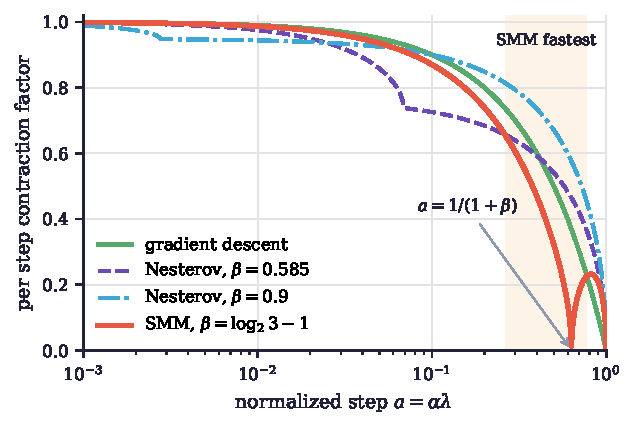
\includegraphics[width=\textwidth]{figures/ch6_contraction.pdf}
  \caption{Per step contraction factor on an eigendirection against
  $a=\alpha\lambda$ (log scale) for gradient descent, every step Nesterov at
  $\beta=0.585$ and $\beta=0.9$, and \smmdet. For \smmdet\ the factor is
  $|(1-a)(1-(1+\beta)a)|^{1/2}$; it vanishes at $a=1/(1+\beta)$ and $a=1$. SMM
  contracts fastest of the four for $0.262<a<0.774$ and is beaten by every step
  momentum in the slow modes.}
  \label{fig:ch6:contraction}
\end{figure}

\begin{table}[t]
\centering
\caption{Per step contraction factor on an eigendirection, $\beta=0.585$ unless
stated. Values computed from the characteristic roots.}
\label{tab:ch6:rates}
\begin{tabular}{ccccc}
\toprule
$a=\alpha\lambda$ & GD & NAG, $\beta=0.585$ & NAG, $\beta=0.9$ & \smmdet\\
\midrule
$0.01$ & $0.9900$ & $0.9754$ & $0.9439$ & $0.9871$\\
$0.04$ & $0.9600$ & $0.8920$ & $0.9295$ & $0.9482$\\
$0.10$ & $0.9000$ & $0.7256$ & $0.9000$ & $0.8703$\\
$0.25$ & $0.7500$ & $0.6624$ & $0.8216$ & $0.6729$\\
$0.50$ & $0.5000$ & $0.5408$ & $0.6708$ & $0.3221$\\
\bottomrule
\end{tabular}
\end{table}

The picture is consistent with the experiments.
On very well conditioned problems every $a=\alpha\lambda$ lies in $[1/\kappa,1]$, and the slowest mode $a=1/\kappa$ falls in the window $0.262<a<0.774$ where \smmdet\ contracts fastest; indeed at $\kappa=2$ it is the fastest method tested.
As $\kappa$ grows the slow
modes dominate and every step momentum\index{momentum} takes over. Nothing here depends on the
Collatz origin of $\beta$; it is the algebra of the polynomial
$\rho$.

\subsection{Chebyshev steps and silver steps}

\Cref{thm:smmquad} invites comparison with the best cyclic schedule of period
two. On a quadratic with spectrum in $[\mu,L]$, the two step polynomial
$(1-h_1\lambda)(1-h_2\lambda)$ that minimizes the maximum modulus over
$[\mu,L]$ is the scaled Chebyshev\index{Chebyshev step sizes} polynomial of degree two; its roots are
\[
  \lambda_\pm=\frac{L+\mu}2\pm\frac{L-\mu}{2\sqrt2},
\]
so $h_\pm=1/\lambda_\pm$, and the worst case two step factor is
$1/T_2\bigl((\kappa+1)/(\kappa-1)\bigr)$~\cite{young1953,golub1961}. As
$\kappa\to\infty$ the ratio of the two steps tends to
$(1+1/\sqrt2)/(1-1/\sqrt2)=(\sqrt2+1)^2=5.83$, the long step approaches
$6.83/L$, and the per step factor is $1-4/\kappa+O(\kappa^{-2})$. We computed,
for example, a per step factor of $0.709$ at $\kappa=10$ and $0.9615$ at
$\kappa=100$, against $0.870$ and $0.9871$ for \smmdet\ with $\alpha=1/L$. SMM is
thus a very conservative member of the period two family: its step ratio
$1+\beta=1.585$ is fixed and its long step is short, so that the scheme is
stable with no knowledge of $\mu$. The Chebyshev schedule needs $\mu$ to place
its roots and is fragile when the estimate is wrong; this is the cyclic step\index{cyclic step sizes}
size version of the retuning problem of \cref{sec:ch6:problem}.

Periodic Chebyshev schedules of a fixed period $p$ cannot change the order of
the iteration count: since $T_p(1+2/\kappa)=1+2p^2/\kappa+O(\kappa^{-2})$, the per
step factor is $1-2p/\kappa+O(\kappa^{-2})$. Altschuler and
Parrilo~\cite{altschuler2024} showed that suitably designed nonperiodic
schedules, built recursively and involving the silver ratio $1+\sqrt2$, do
accelerate gradient descent for smooth convex optimization. We mention this only to locate SMM: it is a fixed period two
schedule and inherits the order $\kappa$ iteration count of gradient descent,
with a better constant.

\subsection{Nonquadratic objectives}

For a general $f$, \cref{lem:ch6:ystep} still says that the even iterates follow
the cyclic schedule exactly, but with the long step \emph{first}:
$x_{t+2}=G_\alpha(G_{(1+\beta)\alpha}(x_t))$. The second statement of
\cref{thm:smmquad}, that $x_{t+2}=G_{(1+\beta)\alpha}(x_{t+1})$ so that the odd
iterates also lie on a cyclic gradient path, used commutation and is only
approximately true. The defect is of third order in the step size.

\begin{proposition}[Order of the defect]\label{prop:ch6:defect}
Suppose $\nabla^2f$ is Lipschitz with constant $M$. For even $t$, with
$h=x_{t+1}-x_t=-\alpha\nabla f(x_t)$,
\begin{multline*}
  x_{t+2}-G_{(1+\beta)\alpha}(x_{t+1})\\
  =\alpha\bigl[(1+\beta)\nabla f(x_{t+1})-\beta\nabla f(x_{t+1}-h)
   -\nabla f(x_{t+1}+\beta h)\bigr],
\end{multline*}
and
\[
  \bigl\|x_{t+2}-G_{(1+\beta)\alpha}(x_{t+1})\bigr\|
  \le\frac{M}{2}\,\beta(1+\beta)\,\alpha^3\,\|\nabla f(x_t)\|^2 .
\]
The bracket vanishes identically when $\nabla f$ is affine.
\end{proposition}

\begin{proof}
By \eqref{eq:ch6:general}, $x_{t+2}=x_{t+1}-\beta\alpha\nabla f(x_t)-\alpha\nabla
f(y_{t+1})$, and $x_t=x_{t+1}-h$, $y_{t+1}=x_{t+1}+\beta h$. Subtracting
$G_{(1+\beta)\alpha}(x_{t+1})=x_{t+1}-(1+\beta)\alpha\nabla f(x_{t+1})$ gives the
displayed identity. Write $u=x_{t+1}$ and $H=\nabla^2f(u)$. Taylor's theorem with
the Lipschitz Hessian gives $\nabla f(u-h)=\nabla f(u)-Hh+r_1$ and
$\nabla f(u+\beta h)=\nabla f(u)+\beta Hh+r_2$ with $\|r_1\|\le\tfrac M2\|h\|^2$
and $\|r_2\|\le\tfrac M2\beta^2\|h\|^2$. The bracket equals $-\beta r_1-r_2$, whose
norm is at most $\tfrac M2(\beta+\beta^2)\|h\|^2$. Multiply by $\alpha$ and use
$\|h\|=\alpha\|\nabla f(x_t)\|$.
\end{proof}

We checked the exact statement numerically on a regularized logistic regression
in five dimensions: the even iterates of \smmdet\ agree with the cyclic schedule
$(1+\beta)\alpha,\alpha$ to $10^{-16}$, while the reversed order agrees only up
to a defect that shrinks with the gradient, from $0.13$ at the first period to
$2\times10^{-8}$ by the fourth. For the purposes of this book the point is
simple: on smooth problems SMM is a period two step size schedule with steps
$(1+\beta)\alpha$ and $\alpha$, observed at two different points of each period.
For $\mu$ strongly convex and $L$ smooth $f$ the same identity gives the linear rate of \cref{thm:ch5b:rate} in \cref{chap:difference}.

\begin{remark}[What the reframing changes]\label{rem:ch6:reframing}
A natural first reading describes the parity schedule as momentum\index{momentum} that is
active half the time, a buffer that is thinned. \Cref{lem:ch6:ystep} shows that
the buffer is never more than one gradient deep, so SMM carries no long memory
at all. This is the structural reason why its noise amplification, computed in
\cref{chap:noise}, stays bounded however close $\beta$ is to one: a cyclic step\index{cyclic step sizes}
size method can only amplify noise through its step lengths, and these are
bounded by $(1+\beta)\alpha<2\alpha$.
\end{remark}

\section*{Notes}

The two derivations of $\beta$ are ours; the log displacement identity is \cref{thm:stride} of
\cref{chap:lyapunov} in Syracuse form, and the Kullback\index{Kullback and Leibler divergence} and Leibler reading is
elementary. The coefficient $\log(3/2)/\log 2=\lt-1$ is the fractional part of
$\lt$, whose continued fraction\index{continued fraction} is the subject of \cref{chap:cycles}; the
present chapter uses only its numerical value.

Polyak's book~\cite{polyak1987} treats heavy ball\index{heavy ball} and Chebyshev\index{Chebyshev step sizes} iterations on
quadratics side by side, and is the best place to see why a period two cyclic
step size method and a momentum\index{momentum} method are close relatives.
For switched linear systems see
Liberzon~\cite{liberzon2003}; for MM algorithm\index{MM algorithm}s, Lange, Hunter and
Yang~\cite{lange2000} and the tutorial~\cite{hunter2004}.

\Cref{thm:smmquad}, \cref{lem:ch6:ystep} and \cref{prop:ch6:defect} are, as far as we know, new in this book, and we regard them as the correct way to think about the method.

\section*{Exercises}

\begin{exercise}
Show that $\KL(U_j\,\|\,U_{j+1})=\log\bigl((j+1)/j\bigr)$ for nested uniform distributions, and that $\KL(U_{j+1}\,\|\,U_j)=\infty$. Show that \[ \log_3 2=\KL(U_1\,\|\,U_2)/\KL(U_1\,\|\,U_3)=1/(1+\beta), \] and that $\KL(U_1\,\|\,U_3)=\KL(U_1\,\|\,U_2)+\KL(U_2\,\|\,U_3)$ is not one of the consecutive divergences. Write the stability limit $1+\log_3 2$ of \cref{cor:ch6:stability} in terms of $\beta$ alone, and explain why its expression in divergences carries no information about stability.
\end{exercise}

\begin{exercise}
For odd $n$ with $\vt(3n+1)=1$, show that $\log S(n)-\log n$ decreases to
$\log(3/2)$ and is at most $\log(5/3)$ for $n\ge3$. Relate the excess over
$\log(3/2)$ to $\varepsilon_n$ in \cref{lem:ch6:logdisp}.
\end{exercise}

\begin{exercise}
Let $0\le\beta<1$, $\beta'\in(0,1)$ and $0<a<1$. Show that every step Nesterov\index{Nesterov acceleration} with coefficient $\beta'$ is underdamped on an eigendirection if and only if $(1-a)(1+\beta')^2<4\beta'$, and that in this regime \smmdet\ has the smaller per step contraction factor if and only if $|1-(1+\beta)a|<\beta'$, that is $(1-\beta')/(1+\beta)<a<(1+\beta')/(1+\beta)$. Verify the crossovers $0.262$ and $0.063$ quoted in the text, and show that for $\beta'\ge\beta$ the upper limit is not reached by any $a<1$.
\end{exercise}

\begin{exercise}
Replace the parity schedule by injection every third step: descend at $t\equiv0,1\pmod3$ and inject at $t\equiv2\pmod3$. Show that, as in \cref{lem:ch6:ystep}, the extrapolated point is a gradient step of length $(1+\beta)\alpha$ from the previous iterate for every differentiable $f$, so that the iterates at $t\equiv0\pmod3$ follow gradient descent with the periodic steps $\alpha,(1+\beta)\alpha,\alpha$, and that the slow mode effective step multiplier is $(3+\beta)/3$. What happens if injection occurs at two consecutive steps? Show that the second extrapolated point then involves gradients at two different points.
\end{exercise}

\begin{exercise}
Take $f(x)=x^4/4$ on $\R$. Starting from $x_0=1$ with $\alpha=1/3$ and
$\beta=\lt-1$, compute two steps of \smmdet\ and compare $x_2$ with
$G_\alpha(G_{(1+\beta)\alpha}(x_0))$ and with $G_{(1+\beta)\alpha}(G_\alpha(x_0))$.
Check the bound of \cref{prop:ch6:defect} with $M=6\sup|x|$ over the relevant
interval.
\end{exercise}

\begin{exercise}
Show that the period two schedule minimizing
$\max_{\lambda\in[\mu,L]}|(1-h_1\lambda)(1-h_2\lambda)|$ has
$h_2/h_1\to(\sqrt2+1)^2$ as $\kappa\to\infty$, and that its worst case per step
factor is $1-4/\kappa+O(\kappa^{-2})$. For which $\kappa$ is the SMM ratio
$h_2/h_1=1+\beta$ optimal?
\end{exercise}

\chapter{Noise, Variance and Experiments}\label{chap:noise}

\Cref{chap:smm} showed that in the noiseless setting the parity schedule of
Switching MM\index{Switching MM} is not an acceleration device. On a quadratic, \smmdet\ is a
period two step size schedule with steps $\alpha$ and $(1+\beta)\alpha$
(\cref{thm:smmquad}); in the slow directions it improves the constant of
gradient descent by the factor $m_{\mathrm{SMM}}=(2+\beta)/2$ and is beaten by
every step momentum\index{momentum}, whose factor is $1/(1-\beta)$. If SMM has a reason to
exist, that reason must lie elsewhere.
A natural hope is that the parity schedule acts as a \emph{variance filter}: momentum recycles gradient shocks through its memory, and a method that uses its memory only half the time ought to recycle less noise.

This chapter puts that hope to an exact test. After recalling the classical
AR(2) analysis of every step momentum under additive gradient noise, we prove
the corresponding exact result for \smmdet, \cref{thm:smmvar}. In the slow
modes SMM amplifies noise, relative to gradient descent at the same step, by
$(2+2\beta+\beta^2)/(2+\beta)$: this is $1.359$ at the Collatz value of
$\beta$ and never exceeds $5/3$, whereas every step momentum amplifies by the
unbounded factor $1/(1-\beta)$.
Compared at matched speed in the slow modes rather than at matched step, SMM has no advantage over gradient descent in those modes, although it is quieter in the fast ones; it is quieter than every step momentum largely because it moves more cautiously.
Its genuine
virtue is robustness: its noise behaviour hardly depends on $\beta$, which is
the precise content of the claim that SMM is a low tuning method.
The second half of the chapter presents experiments with SMM, rerun for this book, and reconciles them quantitatively with the theory.

\section{A model of gradient noise}\label{sec:ch7:model}

We work with the strongly convex quadratic
$f(x)=\tfrac12x^\top Ax-b^\top x$, $A$ symmetric positive definite with
eigenvalues in $[\mu,L]$, and suppose that the algorithm does not see
$\nabla f$ but a noisy version
\begin{equation}\label{eq:ch7:oracle}
  g(x)=\nabla f(x)+\xi,
\end{equation}
where a fresh $\xi$ is drawn at every call, independent of the past, with mean
zero and covariance $\sigma^2I$. This is the simplest model of a stochastic
gradient; it ignores the state dependence and anisotropy of minibatch noise,
but isolates how a method turns independent shocks into fluctuations of the
iterate. Every method we consider decouples along the eigenvectors of $A$. Fix
an eigenvalue $\lambda$, write $a=\alpha\lambda$ for the normalized step,
$e_t$ for the component of $x_t-x^\ast$ and $\xi_t$ for the component of the
noise drawn at iteration $t$; the $\xi_t$ are independent with mean zero and
variance $\sigma^2$. With $\alpha=1/L$, $a$ ranges over $[1/\kappa,1]$. Each
scalar error has a variance that converges to a limit, the \emph{stationary
variance}, and since
\begin{equation}\label{eq:ch7:gap}
  \E\bigl[f(x_t)-f(x^\ast)\bigr]=\tfrac12\sum_{\lambda}\lambda\,\E[e_t(\lambda)^2],
\end{equation}
these limits determine the noise floor\index{noise floor} that remains after the
deterministic transient has died away.

For gradient descent, $e_{t+1}=(1-a)e_t-\alpha\xi_t$, an autoregression of
order one, and the stationary variance is
\begin{equation}\label{eq:ch7:gd}
  V_{\mathrm{GD}}(a)=\frac{\alpha^2\sigma^2}{1-(1-a)^2}
  =\frac{\alpha^2\sigma^2}{a(2-a)},\qquad 0<a<2.
\end{equation}
In the slow modes $V_{\mathrm{GD}}\approx\alpha^2\sigma^2/(2a)=\alpha\sigma^2/(2\lambda)$:
the floor is proportional to the step. A longer step is faster and noisier in
exactly compensating amounts, and every comparison below must account for
this.

\section{Every step momentum as an autoregression}\label{sec:ch7:ar2}

\subsection{The stationary variance of an AR(2) process}

The classical tool is an elementary lemma on autoregressions of order two;
see Brockwell\index{Brockwell, P. J.} and Davis\index{Davis, R. A.}~\cite{brockwell1991} for the general theory.

\begin{lemma}[Stationary variance of an AR(2) process]\label{lem:ch7:ar2}
Let $e_{t+1}=a_1e_t+a_2e_{t-1}+\varepsilon_t$ with $\varepsilon_t$ independent,
mean zero, variance $s^2$, and $\varepsilon_t$ independent of
$(e_t,e_{t-1})$. Suppose both roots of $z^2-a_1z-a_2$ lie in the open unit
disc, which holds if and only if
\begin{equation}\label{eq:ch7:triangle}
  |a_2|<1,\qquad 1-a_1-a_2>0,\qquad 1+a_1-a_2>0 .
\end{equation}
Then $\Var(e_t)$ converges, from any initial condition with finite second
moments, to
\begin{equation}\label{eq:ch7:ar2var}
  \gamma_0=\frac{(1-a_2)\,s^2}{(1+a_2)\bigl((1-a_2)^2-a_1^2\bigr)} .
\end{equation}
\end{lemma}

\begin{proof}
In state form the covariance of $(e_t,e_{t-1})$ obeys an affine recursion
whose linear part has spectral radius equal to the square of that of the
companion matrix, which is less than one; so it converges geometrically to its
unique fixed point. In stationarity let $\gamma_k=\Cov(e_t,e_{t-k})$.
Multiplying the recursion by $e_t$, by $e_{t-1}$ and by $e_{t+1}$ and taking expectations
gives the Yule and Walker equations
\[
  \gamma_1=a_1\gamma_0+a_2\gamma_1,\qquad
  \gamma_2=a_1\gamma_1+a_2\gamma_0,\qquad
  \gamma_0=a_1\gamma_1+a_2\gamma_2+s^2 .
\]
The first gives $\gamma_1=a_1\gamma_0/(1-a_2)$. Substituting the second into
the third, $\gamma_0(1-a_2^2)=a_1(1+a_2)\gamma_1+s^2
=a_1^2(1+a_2)\gamma_0/(1-a_2)+s^2$. Multiplying by $1-a_2$ and collecting terms
gives $\gamma_0(1+a_2)\bigl((1-a_2)^2-a_1^2\bigr)=(1-a_2)s^2$, which is
\eqref{eq:ch7:ar2var}. The conditions \eqref{eq:ch7:triangle} are the classical
stability triangle for a real quadratic.
\end{proof}

\subsection{Heavy ball}

The noisy heavy ball\index{heavy ball} iteration
$x_{t+1}=x_t-\alpha g(x_t)+\beta(x_t-x_{t-1})$ gives, on an eigendirection,
\begin{equation}\label{eq:ch7:hbrec}
  e_{t+1}=(1+\beta-a)\,e_t-\beta\,e_{t-1}-\alpha\xi_t,
\end{equation}
an AR(2) process with $a_1=1+\beta-a$, $a_2=-\beta$ and $s^2=\alpha^2\sigma^2$.

\begin{proposition}[Heavy ball under additive noise]\label{prop:ch7:hb}
Let $0\le\beta<1$ and $0<a<2(1+\beta)$. The stationary variance of
\eqref{eq:ch7:hbrec} is
\begin{equation}\label{eq:ch7:hbvar}
  V_{\mathrm{HB}}(a)=\frac{\alpha^2\sigma^2\,(1+\beta)}{(1-\beta)\,a\,\bigl(2(1+\beta)-a\bigr)} .
\end{equation}
As $a\to0$, $V_{\mathrm{HB}}(a)\sim\alpha^2\sigma^2/\bigl(2a(1-\beta)\bigr)$, so
$V_{\mathrm{HB}}/V_{\mathrm{GD}}\to1/(1-\beta)$.
\end{proposition}

\begin{proof}
The conditions \eqref{eq:ch7:triangle} read $\beta<1$, $1-a_1-a_2=a>0$ and
$1+a_1-a_2=2(1+\beta)-a>0$, which are the hypotheses. In
\eqref{eq:ch7:ar2var}, $1-a_2=1+\beta$, $1+a_2=1-\beta$, and
\[
  (1-a_2)^2-a_1^2=(1+\beta)^2-(1+\beta-a)^2=a\bigl(2(1+\beta)-a\bigr).
\]
This is \eqref{eq:ch7:hbvar}. For small $a$ the last factor is
$2(1+\beta)+O(a)$, the factors $1+\beta$ cancel, and the limit follows on
dividing by $V_{\mathrm{GD}}\sim\alpha^2\sigma^2/(2a)$.
\end{proof}

The factor $1/(1-\beta)$ is $2.409$ at $\beta=\lt-1$, $3$ at $\beta=2/3$ and $10$
at $\beta=0.9$. Its origin is easy to see. In the slow regime the characteristic
polynomial has a fast root near $\beta$ and a slow root $1-a/(1-\beta)+O(a^2)$.
A shock $\alpha\xi_t$ enters the velocity, and by the time the fast root has
dissipated it the position has moved by
$\alpha\xi_t(1+\beta+\beta^2+\cdots)=\alpha\xi_t/(1-\beta)$. Momentum thus
multiplies the effective step by $m=1/(1-\beta)$, speeding the slow mode up by
$m$, and multiplies each shock by $m$, hence its variance by $m^2$; the net
effect on the floor is $m^2/m=m$. We return to this bookkeeping in
\cref{sec:ch7:efficiency}.

\subsection{Nesterov}

Constant momentum\index{momentum} Nesterov\index{Nesterov acceleration} evaluates the noisy gradient at the extrapolated
point: $y_t=x_t+\beta(x_t-x_{t-1})$, $x_{t+1}=y_t-\alpha g(y_t)$. On an
eigendirection,
\begin{equation}\label{eq:ch7:nagrec}
  e_{t+1}=(1-a)(1+\beta)\,e_t-(1-a)\beta\,e_{t-1}-\alpha\xi_t .
\end{equation}

\begin{proposition}[Nesterov under additive noise]\label{prop:ch7:nag}
Let $0\le\beta<1$ and $0<a\le1$. The stationary variance of
\eqref{eq:ch7:nagrec} is
\begin{equation}\label{eq:ch7:nagvar}
  V_{\mathrm{NAG}}(a)=\frac{\alpha^2\sigma^2\,(1+\beta-a\beta)}
  {a\,(1-\beta+a\beta)\,\bigl(2(1+\beta)-a(1+2\beta)\bigr)} .
\end{equation}
As $a\to0$, $V_{\mathrm{NAG}}/V_{\mathrm{GD}}\to1/(1-\beta)$, the same slow mode
amplification as heavy ball\index{heavy ball}; at $a=1$, $V_{\mathrm{NAG}}=V_{\mathrm{GD}}=\alpha^2\sigma^2$.
\end{proposition}

\begin{proof}
Here $a_1=(1-a)(1+\beta)$ and $a_2=-(1-a)\beta$, so $|a_2|<1$,
$1-a_1-a_2=1-(1-a)=a>0$ and $1+a_1-a_2=1+(1-a)(1+2\beta)>0$; the lemma applies.
Now $1-a_2=1+\beta-a\beta$, $1+a_2=1-\beta+a\beta$, and
\[
  (1-a_2)^2-a_1^2=(1-a_2-a_1)(1-a_2+a_1)=a\bigl(2(1+\beta)-a(1+2\beta)\bigr)
\]
since $1-a_2+a_1=1+\beta-a\beta+(1-a)(1+\beta)=2(1+\beta)-a(1+2\beta)$.
Substituting in \eqref{eq:ch7:ar2var} gives \eqref{eq:ch7:nagvar}, and both
limits are immediate.
\end{proof}

Heavy ball and Nesterov agree in the slow modes and differ for larger $a$: at
$a=1$ the Nesterov error is just the last shock, while heavy ball still carries
momentum.

\section{The exact variance of Switching MM}\label{sec:ch7:smmvar}

For \smmdet\ the coefficients alternate with the parity of $t$, so the error is
not a stationary AR(2) process. The way through is \cref{lem:ch6:ystep}, which
holds for any gradient oracle and therefore for the noisy one: starting from an
even index, the extrapolated point is a single long step from $x_t$ using the
\emph{same} noisy gradient,
\[
  y_{t+1}=x_{t+1}+\beta(x_{t+1}-x_t)=x_t-(1+\beta)\alpha\,g(x_t).
\]
The noise drawn at the even step is therefore used twice, once in the descent
step and once more, scaled by $\beta$, through the extrapolation. Two steps of
SMM consume two independent shocks with weights $(1+\beta)\alpha$ and $\alpha$,
exactly as noisy gradient descent with the cyclic step\index{cyclic step sizes}s $(1+\beta)\alpha$ and
$\alpha$ would.

\begin{theorem}[Stationary variance of \smmdet]\label{thm:smmvar}
Let $f$ be the quadratic of \cref{sec:ch7:model}, with the noisy oracle
\eqref{eq:ch7:oracle}, let $0\le\beta<1$, and fix an eigendirection with
$a=\alpha\lambda\in(0,1]$. Let
\[
  \rho=(1-a)\bigl(1-(1+\beta)a\bigr).
\]
\begin{enumerate}[label=(\roman*),leftmargin=2em]
\item For every even $t$ the error of \smmdet\ satisfies the exact two step
recursion
\begin{equation}\label{eq:ch7:twostep}
  e_{t+2}=\rho\,e_t+w_t,\qquad
  w_t=-(1-a)(1+\beta)\alpha\,\xi_t-\alpha\,\xi_{t+1},
\end{equation}
where the $w_t$, $t$ even, are independent, independent of $e_t$, with mean zero and
$\Var(w_t)=\alpha^2\sigma^2\bigl[(1-a)^2(1+\beta)^2+1\bigr]$.
\item As $t\to\infty$ through even values, $\Var(e_t)$ converges to
\begin{equation}\label{eq:ch7:veven}
  V_{\mathrm{even}}=\frac{\alpha^2\sigma^2\bigl[(1-a)^2(1+\beta)^2+1\bigr]}{1-\rho^2},
\end{equation}
and through odd values to
\begin{equation}\label{eq:ch7:vodd}
  V_{\mathrm{odd}}=(1-a)^2\,V_{\mathrm{even}}+\alpha^2\sigma^2 .
\end{equation}
\item The phase averaged stationary variance
$V_{\mathrm{SMM}}=\tfrac12(V_{\mathrm{even}}+V_{\mathrm{odd}})$ is the rational
function
\begin{equation}\label{eq:ch7:vavg}
  \frac{V_{\mathrm{SMM}}(a)}{\alpha^2\sigma^2}
  =\frac{Q(a,\beta)}{1-\rho^2},
\end{equation}
with
\begin{align*}
  Q(a,\beta)&=(2+2\beta+\beta^2)-(1+\beta)(2+3\beta)\,a\\
  &\quad+(1+\beta)(1+3\beta)\,a^2-\beta(1+\beta)\,a^3,\\
  1-\rho^2&=a\bigl(2+\beta-(1+\beta)a\bigr)\bigl(2-(2+\beta)a+(1+\beta)a^2\bigr).
\end{align*}
\end{enumerate}
\end{theorem}

\begin{proof}
(i) Let $t$ be even. The descent step gives
$e_{t+1}=(1-a)e_t-\alpha\xi_t$, so $e_{t+1}-e_t=-ae_t-\alpha\xi_t$ and the
extrapolated point has error
\[
  e_{t+1}+\beta(e_{t+1}-e_t)
  =\bigl(1-(1+\beta)a\bigr)e_t-(1+\beta)\alpha\xi_t .
\]
The injection step evaluates a noisy gradient at this point, with fresh noise
$\xi_{t+1}$, and multiplies the error by $1-a$:
\[
  e_{t+2}=(1-a)\bigl[\bigl(1-(1+\beta)a\bigr)e_t-(1+\beta)\alpha\xi_t\bigr]-\alpha\xi_{t+1},
\]
which is \eqref{eq:ch7:twostep}. The error $e_t$ is a function of $e_0$ and of
$\xi_0,\dots,\xi_{t-1}$, while $w_t$ is a function of $\xi_t$ and $\xi_{t+1}$;
for distinct even $t$ the pairs $(\xi_t,\xi_{t+1})$ are disjoint. This gives the
independence claims, and the variance of $w_t$ is the sum of the variances of its
two independent terms.

(ii) By (i), $\Var(e_{t+2})=\rho^2\Var(e_t)+\Var(w_t)$ for even $t$. By
\cref{cor:ch6:stability}, $|\rho|<1$ whenever $0<a<(2+\beta)/(1+\beta)$, in
particular for $a\in(0,1]$, so this affine recursion converges geometrically to
its fixed point \eqref{eq:ch7:veven}. For odd times, $e_{t+1}=(1-a)e_t-\alpha\xi_t$
with $\xi_t$ independent of $e_t$, so $\Var(e_{t+1})=(1-a)^2\Var(e_t)+\alpha^2\sigma^2$,
and \eqref{eq:ch7:vodd} follows by letting $t\to\infty$ through even values.

(iii) We have $V_{\mathrm{SMM}}=\tfrac12\bigl[(1+(1-a)^2)V_{\mathrm{even}}+\alpha^2\sigma^2\bigr]$.
The factorization of $1-\rho^2$ comes from
$1-\rho=a(2+\beta-(1+\beta)a)$ and $1+\rho=2-(2+\beta)a+(1+\beta)a^2$. Over
the common denominator $1-\rho^2$ the numerator is
$\tfrac12\bigl[(1+(1-a)^2)\bigl((1-a)^2(1+\beta)^2+1\bigr)+1-\rho^2\bigr]$, and
expanding this polynomial in $a$ gives $Q(a,\beta)$. We checked the expansion
with a computer algebra system, which confirms that \eqref{eq:ch7:vavg} agrees
identically with the definition of $V_{\mathrm{SMM}}$.
\end{proof}

The even subsequence is thus an autoregression of order one: the second state
variable of every step momentum\index{momentum} has disappeared, because the descent step
forgets $e_{t-1}$, and the noise of the even step is amplified by $1+\beta<2$
and no more.

\subsection{The slow mode limit}

\begin{corollary}[Slow mode amplification]\label{cor:ch7:slow}
As $a\to0$, both $aV_{\mathrm{even}}$ and $aV_{\mathrm{odd}}$ converge to
\[
  \alpha^2\sigma^2\,\frac{(1+\beta)^2+1}{2(2+\beta)}
  =\alpha^2\sigma^2\,\frac{1+\beta+\beta^2/2}{2+\beta}.
\]
Consequently
\begin{equation}\label{eq:ch7:V}
  \lim_{a\to0}\frac{V_{\mathrm{SMM}}(a)}{V_{\mathrm{GD}}(a)}
  =V(\beta):=\frac{2+2\beta+\beta^2}{2+\beta}=\beta+\frac{2}{2+\beta}.
\end{equation}
\end{corollary}

\begin{proof}
From \eqref{eq:ch7:veven}, $1-\rho^2=a(2+\beta)\cdot2+O(a^2)$ and the
numerator tends to $\alpha^2\sigma^2\bigl[(1+\beta)^2+1\bigr]$, which gives the
limit for $aV_{\mathrm{even}}$. By \eqref{eq:ch7:vodd},
$aV_{\mathrm{odd}}=(1-a)^2aV_{\mathrm{even}}+a\alpha^2\sigma^2$ has the same limit.
Since $(1+\beta)^2+1=2+2\beta+\beta^2$ and $aV_{\mathrm{GD}}\to\alpha^2\sigma^2/2$,
the ratio tends to $(2+2\beta+\beta^2)/(2+\beta)$. Finally
$(2+\beta)\beta+2=2+2\beta+\beta^2$.
\end{proof}

The formula has a transparent reading in terms of the cyclic step\index{cyclic step sizes} size picture.
Write the two steps of a period as $h_1\alpha$ and $h_2\alpha$ with
$h_1=1+\beta$ and $h_2=1$. In the slow modes one period contracts the error by
$1-(h_1+h_2)a$ and injects noise of variance $(h_1^2+h_2^2)\alpha^2\sigma^2$, so
the stationary variance is approximately
$(h_1^2+h_2^2)\alpha^2\sigma^2/\bigl(2(h_1+h_2)a\bigr)$. Dividing by the gradient
descent value $\alpha^2\sigma^2/(2a)$ gives
\begin{equation}\label{eq:ch7:Vh}
  V(\beta)=\frac{(h_1^2+h_2^2)/2}{(h_1+h_2)/2}
  =\frac{\text{mean square step}}{\text{mean step}} .
\end{equation}
For every step momentum\index{momentum} the same bookkeeping, with effective step $m=1/(1-\beta)$
and shocks multiplied by $m$, gave $m^2/m=m$. The difference between the two
methods is that SMM never lengthens any single step by more than the factor
$1+\beta<2$.

\begin{proposition}[Uniform bound in $\beta$]\label{prop:ch7:bound}
The function $V(\beta)=\beta+2/(2+\beta)$ is strictly increasing on $[0,1]$,
with $V(0)=1$ and $V(1)=5/3$. Hence
\[
  1\le V(\beta)<\tfrac53\qquad\text{for all }0\le\beta<1,
\]
whereas the every step amplification $1/(1-\beta)$ tends to infinity as
$\beta\to1$.
\end{proposition}

\begin{proof}
$V'(\beta)=1-2/(2+\beta)^2$, and $(2+\beta)^2\ge4>2$ for $\beta\ge0$, so
$V'>0$. The values at the endpoints are $0+1=1$ and $1+2/3=5/3$.
\end{proof}

At $\beta=\lt-1$ the slow mode amplification is $V=1.359$, against $2.409$ for
every step momentum at the same coefficient. At $\beta=0.9$ it is $1.590$,
against $10$. The slow modes are the worst case, as the next result shows: the
bound $V(\beta)$ holds on every eigendirection, not only in the limit.

\begin{proposition}[The slow mode bound is uniform in $a$]\label{prop:ch7:uniform}
For $0\le\beta<1$ and every $a\in(0,1]$,
\[
  V_{\mathrm{GD}}(a)\le V_{\mathrm{SMM}}(a)\le V(\beta)\,V_{\mathrm{GD}}(a)<\tfrac53\,V_{\mathrm{GD}}(a),
\]
with $V_{\mathrm{SMM}}(a)=V_{\mathrm{GD}}(a)$ only when $\beta=0$ or $a=1$, and $V_{\mathrm{SMM}}(a)=V(\beta)V_{\mathrm{GD}}(a)$ only when $\beta=0$.
\end{proposition}

\begin{proof}
Write $\rho=(1-a)(1-(1+\beta)a)$ as before. A direct computation from
\eqref{eq:ch7:gd} and \eqref{eq:ch7:vavg}, which we verified by computer
algebra, gives
\begin{multline*}
  \frac{V(\beta)V_{\mathrm{GD}}(a)-V_{\mathrm{SMM}}(a)}{\alpha^2\sigma^2}\\
  =\frac{\beta(1+\beta)\,\bigl(-P(a,\beta)\bigr)}
  {(2-a)(2+\beta)\bigl(2+\beta-(1+\beta)a\bigr)(1+\rho)},
\end{multline*}
where
\[
  P(a,\beta)=(2+\beta)a^3-(7+2\beta-\beta^2)a^2+(10+\beta-2\beta^2)a-(6-\beta^2).
\]
For $a\in(0,1]$ all four factors of the denominator are positive: $2-a>0$,
$2+\beta>0$, $2+\beta-(1+\beta)a\ge1>0$, and $1+\rho>0$ by
\cref{cor:ch6:stability}. It remains to show $P<0$. Since
$(2+\beta)a^3\le(2+\beta)a^2$ for $a\le1$,
\[
  P(a,\beta)\le q(a):=-(5+\beta-\beta^2)a^2+(10+\beta-2\beta^2)a-(6-\beta^2).
\]
The quadratic $q$ has negative leading coefficient, because $5+\beta-\beta^2>0$
on $[0,1]$, and discriminant
\[
  (10+\beta-2\beta^2)^2-4(5+\beta-\beta^2)(6-\beta^2)=5\beta^2-4\beta-20,
\]
which is at most $5-20<0$ on $[0,1]$.
Hence $q<0$ for every real $a$, so $P<0$, and the displayed difference is
nonnegative, and positive when $\beta>0$.
The last inequality is \cref{prop:ch7:bound}.
For the first, the same computation gives
\[
  \frac{V_{\mathrm{SMM}}(a)-V_{\mathrm{GD}}(a)}{\alpha^2\sigma^2}
  =\frac{\beta(1+\beta)(1-a)^2\bigl((1-a)^2+1\bigr)}{a(2-a)\bigl(2+\beta-(1+\beta)a\bigr)(1+\rho)},
\]
whose denominator is positive for $a\in(0,1]$, as above, and whose numerator is nonnegative and vanishes only when $\beta=0$ or $a=1$ (script \texttt{ch7\_extra.py}).
\end{proof}

\begin{remark}[A tempting but incomplete argument]\label{rem:ch7:heuristic}
A natural first argument for the parity schedule runs as follows. Since the
momentum term is active on only half of the iterations, the slow mode
amplification $1/(1-\beta)$ should be roughly halved, to $1.20$ at
$\beta=0.585$. This is close to the exact $1.359$ but not equal to it. At
$\beta=0.9$ it predicts $5$, against the exact $1.590$; as $\beta\to1$ it
predicts an unbounded amplification, against the exact bound $5/3$. The
heuristic treats the parity schedule as a thinned version of a long memory,
whereas \cref{lem:ch6:ystep} shows that SMM has no long memory at all: its
buffer never holds more than the last gradient. What the schedule controls is
not how often noise enters a buffer but how long each step is, and the correct
amplification is the ratio \eqref{eq:ch7:Vh} of mean square to mean step length.
\end{remark}

\section{What the variance buys: efficiency at matched speed}\label{sec:ch7:efficiency}

A smaller noise floor\index{noise floor} at a fixed step size is not by itself an advantage. Any
method can lower its floor by moving more slowly, and gradient descent with a
shorter step is the simplest example.
One fair comparison is between methods run at the same speed in the slow modes, which determine the iteration count.
They do not determine the floor of the objective: by \eqref{eq:ch7:gap} an eigendirection contributes $\tfrac12\lambda V_{\mathrm{GD}}=\alpha\sigma^2/\bigl(2(2-a)\bigr)$ for gradient descent, between $\alpha\sigma^2/4$ and $\alpha\sigma^2/2$, so every eigendirection contributes to the floor on the same scale.
The comparison below concerns each slow eigendirection, not the total floor.
Recall from \cref{cor:ch6:slow} and the discussion following it the effective
step multipliers
\[
  m_{\mathrm{GD}}=1,\qquad m_{\mathrm{HB}}=m_{\mathrm{NAG}}=\frac1{1-\beta},\qquad
  m_{\mathrm{SMM}}=\frac{2+\beta}{2}.
\]
Gradient descent with step $m\alpha$ has slow mode variance
$m\alpha^2\sigma^2/(2a)$, that is $m$ times the floor at step $\alpha$. So the
natural figure of merit is the amplification divided by the speed multiplier,
the \emph{noise floor at matched speed}.

\begin{proposition}[Noise floor at matched speed]\label{prop:ch7:matched}
In the slow mode limit, the noise floor at matched speed relative to gradient
descent is $1$ for heavy ball\index{heavy ball} and for Nesterov\index{Nesterov acceleration}, and for \smmdet\ it is
\[
  \frac{V(\beta)}{m_{\mathrm{SMM}}}=\frac{2(2+2\beta+\beta^2)}{(2+\beta)^2}
  =1+\frac{\beta^2}{(2+\beta)^2}\;\ge\;1 .
\]
It equals $1.051$ at $\beta=\lt-1$ and increases to $10/9$ as $\beta\to1$.
More generally, for any period two schedule with steps $h_1\alpha$ and
$h_2\alpha$ the ratio is $\tfrac12(h_1^2+h_2^2)\big/\bigl(\tfrac12(h_1+h_2)\bigr)^2\ge1$,
with equality only for equal steps.
\end{proposition}

\begin{proof}
For heavy ball and Nesterov the amplification and the speed multiplier are
both $1/(1-\beta)$ (\cref{prop:ch7:hb,prop:ch7:nag}). For SMM, divide
\eqref{eq:ch7:V} by $(2+\beta)/2$ and use $2(2+2\beta+\beta^2)=(2+\beta)^2+\beta^2$.
The function $\beta^2/(2+\beta)^2$ is increasing with value $1/9$ at $\beta=1$.
The general statement is the inequality between the mean square and the
square of the mean, which follows from \eqref{eq:ch7:Vh}.
\end{proof}

This is what the variance theory says. In the slow modes of a
quadratic, gradient descent, heavy ball and Nesterov all sit on the same
efficiency frontier, trading speed for noise one for one. SMM sits slightly \emph{behind} that frontier, by five percent at the
Collatz coefficient, because a cyclic schedule with unequal steps wastes a
little variance relative to a constant schedule of the same mean.
Gradient descent with step $(1+\beta/2)\alpha$ would be as fast as SMM in the slow modes and slightly quieter in them, but noisier in the fast modes, where its longer step costs more than the parity schedule does (\cref{sec:ch7:reconcile}).
So the lower floor of SMM at a fixed $\alpha$, compared
with every step momentum\index{momentum}, comes largely from its smaller effective step,
$1.29\alpha$ against $2.41\alpha$; it is not a free lunch.

What then is the virtue of SMM? It is the uniformity of \cref{prop:ch7:bound,prop:ch7:uniform}.
For every step momentum the cost of a badly chosen large $\beta$ is unbounded:
the floor at step $1/L$ is multiplied by $1/(1-\beta)$, which is $10$ at the
popular default and $100$ at $\beta=0.99$. For SMM the floor at step $1/L$ lies between that of gradient descent and
$5/3$ of it for \emph{every} $\beta\in[0,1)$, and on every eigendirection.
Equally, the speed multiplier lies in $[1,3/2)$. Switching from $\beta=0.585$
to $\beta=0.9$ changes the slow mode floor of every step momentum by a factor
$4.15$ and that of SMM by $17$ percent. SMM is a conservative method: it can
neither gain much nor lose much by the choice of $\beta$, and it is stable for
every $\beta<1$ at the step $1/L$ (\cref{cor:ch6:stability}). That is the
precise sense in which it is a low tuning default.

\begin{remark}[Fixed step versus fixed budget]\label{rem:ch7:budget}
In practice methods are compared at the same $\alpha=1/L$ and the same number
of iterations, which is the protocol of the experiments below. Under that
protocol a method that is both faster and noisier can lose on the final gap,
and a method that is slower and quieter can win, without either being more
efficient in the sense of \cref{prop:ch7:matched}. The experiments therefore
measure a mixture of speed and floor. The theory tells us how to unmix them.
\end{remark}

\section{Numerical illustration and simulation check}\label{sec:ch7:numerics}

\Cref{tab:ch7:ratios} gives the exact ratio of the stationary variance of each
method to that of gradient descent at the same $a$, computed from
\eqref{eq:ch7:gd}, \eqref{eq:ch7:hbvar}, \eqref{eq:ch7:nagvar} and
\eqref{eq:ch7:vavg}. The SMM ratio stays below $V(\beta)$, as
\cref{prop:ch7:uniform} asserts, and falls to $1$ at $a=1$; the Nesterov\index{Nesterov acceleration} ratio
falls from $1/(1-\beta)$ to $1$; the heavy ball\index{heavy ball} ratio decreases only moderately, from $1/(1-\beta)$ to $(1+\beta)/\bigl((1-\beta)(1+2\beta)\bigr)$ at $a=1$, which is $1.760$ at $\beta=\lt-1$, about $30$ percent below the slow mode value.

\begin{table}[tbp]
\centering
\caption{Stationary variance relative to gradient descent at the same
normalized step $a=\alpha\lambda$, from the exact formulas. The last row gives
the slow mode limits $1/(1-\beta)$ and $V(\beta)$.}
\label{tab:ch7:ratios}
\begin{tabular}{ccccccc}
\toprule
 & \multicolumn{3}{c}{$\beta=0.585$} & \multicolumn{3}{c}{$\beta=0.9$}\\
\cmidrule(lr){2-4}\cmidrule(lr){5-7}
$a$ & NAG & HB & \smmdet & NAG & HB & \smmdet\\
\midrule
$0.001$ & $2.406$ & $2.409$ & $1.358$ & $9.908$ & $9.998$ & $1.589$\\
$0.01$  & $2.372$ & $2.405$ & $1.355$ & $9.153$ & $9.976$ & $1.584$\\
$0.04$  & $2.264$ & $2.391$ & $1.343$ & $7.284$ & $9.904$ & $1.568$\\
$0.1$   & $2.074$ & $2.364$ & $1.319$ & $5.142$ & $9.757$ & $1.535$\\
$0.25$  & $1.707$ & $2.289$ & $1.256$ & $2.909$ & $9.366$ & $1.445$\\
$0.5$   & $1.314$ & $2.145$ & $1.146$ & $1.648$ & $8.636$ & $1.267$\\
$1$     & $1.000$ & $1.760$ & $1.000$ & $1.000$ & $6.786$ & $1.000$\\
\midrule
$a\to0$ & $2.409$ & $2.409$ & $1.359$ & $10.00$ & $10.00$ & $1.590$\\
\bottomrule
\end{tabular}
\end{table}

\Cref{fig:ch7:amplification} plots the two slow mode amplification curves
against $\beta$, with simulated ratios from $4000$ independent chains of the
scalar recursions at $a=0.01$; at the five values of $\beta$ shown, the
simulated and exact ratios differ by at most $0.006$ for SMM and $0.004$ for
Nesterov (script \texttt{ch7\_variance.py}). A single long chain of \smmdet\ at $a=0.02$ and $\beta=\lt-1$, run
for $2\times10^6$ steps with unit noise, gave a sample variance of $34.16$,
against the exact phase averaged value $34.11$ and the slow mode approximation
$V(\beta)/(2a)=33.97$ (script \texttt{smm\_sim.py}).

\begin{figure}[tbp]
  \centering
  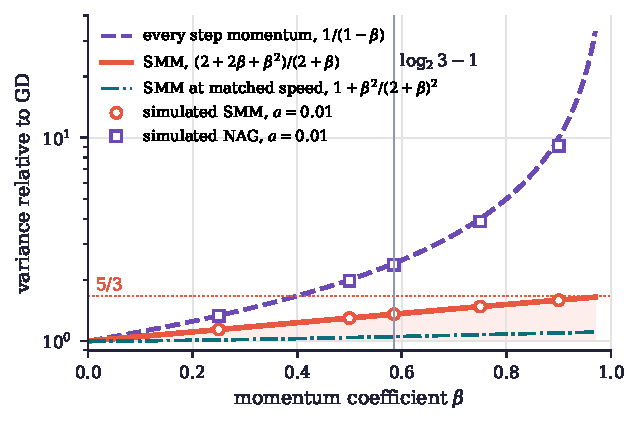
\includegraphics[width=0.85\textwidth]{figures/ch7_amplification.pdf}
  \caption{Slow mode variance amplification relative to gradient descent at the
  same step, as a function of the momentum coefficient (log scale). Dashed:
  every step momentum, $1/(1-\beta)$. Solid: \smmdet,
  $(2+2\beta+\beta^2)/(2+\beta)$, bounded by $5/3$ (dotted); the shaded band lies between $1$ and this curve.
  Dash dotted: \smmdet\ at matched speed, $1+\beta^2/(2+\beta)^2$ (\cref{prop:ch7:matched}).
  Markers: simulated
  ratios at $a=0.01$. The vertical line marks $\beta=\lt-1$.}
  \label{fig:ch7:amplification}
\end{figure}

\section{Beyond period two: the gain weight theorem}\label{sec:ch7:gainweight}

\Cref{prop:ch7:matched} compared \smmdet\ with gradient descent at matched speed
and found a small penalty, $1+\beta^2/(2+\beta)^2$. Is that penalty an accident
of the particular schedule, or would some other pattern of injections, of
period three or four, or with injection on several residues, beat gradient
descent? This is problem P6 of \cref{chap:open}. The answer is no, and the
reason is a single structural fact: in any first order method the noise enters
exactly where the gradient enters.

\paragraph{Setting.} Fix a period $p$ and a memory length $K$. On one
eigendirection of a quadratic, with $a=\alpha\lambda$ and state
$z_t=(e_t,\dots,e_{t-K+1})$, a \emph{linear periodic first order method}
evaluates at step $t$ (with residue $j=t\bmod p$) a gradient at an
extrapolated point $y_t=\gamma_j\cdot z_t$ and updates
\begin{equation}\label{eq:ch7:general}
  e_{t+1}=\delta_j\cdot z_t-h_j\bigl(a\,y_t+\alpha\,\xi_t\bigr),
\end{equation}
with fixed vectors $\gamma_j,\delta_j\in\R^K$ and step multipliers
$h_j>0$, where $\xi_t$ is the gradient noise. Consistency requires that
constants are preserved when the gradient vanishes, $\delta_j\cdot\iota=\gamma_j\cdot\iota=1$,
where $\iota=(1,\dots,1)$. Gradient descent, heavy ball\index{heavy ball}, Nesterov\index{Nesterov acceleration} at every
step, \smmdet, cyclic step\index{cyclic step sizes} sizes, and momentum\index{momentum} applied on any subset of the
residues modulo $p$ are all of this form.
Write $B(a)=B_0+aB_1+O(a^2)$ for the product of the $p$ step matrices over one period, and assume the method is \emph{stable at $a=0$}: the eigenvalue
$1$ of $B_0$, with right eigenvector $\iota$, is simple, and all other
eigenvalues of $B_0$ lie strictly inside the unit disc.

\begin{definition}[Gains]\label{def:ch7:gains}
Let $w$ be the left eigenvector of $B_0$ for the eigenvalue $1$, normalized so
that $w\cdot\iota=1$. The \emph{gain} $c_i$ of the gradient evaluated at
residue $i$ is the total long run effect, at $a=0$, of a unit injection
$-h_i$ into $e$ at that step, measured in the slow coordinate $w\cdot z$:
$c_i=h_i\,w\cdot\Pi_iu_1$, where $u_1$ is the first unit vector and $\Pi_i$ the product of the step matrices at $a=0$ from the step after $i$ to the end of the period. Put $M=\sum_{i=1}^pc_i$.
\end{definition}

The proof of part (i) of the theorem below shows that, whatever the sign of $M$, the period product has the eigenvalue $1-Ma+O(a^2)$, so $M\ge0$ is necessary for stability at small $a>0$. We assume $M>0$; this holds whenever all gains are positive, as for every method listed above with $\beta\in[0,1)$.

For gradient descent $c=1$; for every step momentum $c=1/(1-\beta)$, since a
unit impulse is carried forward with weights $1,\beta,\beta^2,\dots$; for
\smmdet\ the gains are $(1+\beta,\,1)$, because the gradient taken at a descent
step also enters the next extrapolation.

\begin{theorem}[Gain weight theorem]\label{thm:ch7:gainweight}\index{gain weight theorem}
For a linear periodic first order method \eqref{eq:ch7:general} that is stable at $a=0$ and has $M>0$, with
uncorrelated noise of variance $\sigma^2$, as $a\to0$:
\begin{enumerate}[label=(\roman*),leftmargin=2em]
\item the per step contraction of the slow mode is $1-(M/p)\,a+O(a^2)$;
\item the phase averaged stationary variance of $e_t$ is
  $\alpha^2\sigma^2\,\dfrac{\sum_ic_i^2}{2Ma}\,(1+o(1))$;
\item consequently the noise floor relative to gradient descent run at the same
  slow mode speed, step $(M/p)\alpha$, is
  \begin{equation}\label{eq:ch7:F}
    \mathcal F=\frac{p\sum_{i=1}^pc_i^2}{\bigl(\sum_{i=1}^pc_i\bigr)^2}\;\geq\;1,
  \end{equation}
  with equality if and only if all gains are equal.
\end{enumerate}
\end{theorem}

\begin{proof}
Let $s_t=w\cdot z_t$ at the start of each period. Since $w$ is a left
eigenvector of $B_0$, $s$ is unchanged by $B_0$, and over one period
\[
  s_{t+p}=s_t+a\,w\cdot B_1z_t-\alpha\sum_{i=1}^p c_i\,\xi_{t+i-1}+O(a\alpha)\,\|\xi\|,
\]
where the noise coefficients are the gains by \cref{def:ch7:gains}. The key
observation is that the deterministic term has the same coefficients. The
gradient enters \eqref{eq:ch7:general} through $h_j(a\,y_t+\alpha\xi_t)$,
so replacing $\alpha\xi_t$ by $a\,y_t$ shows that $a\,w\cdot B_1z_t=-a\sum_i
c_i\,y_{t+i-1}+O(a^2)\|z\|$. On the slow manifold $z\approx s\iota$ we have
$y\approx s$, because $\gamma_j\cdot\iota=1$, and therefore
$w\cdot B_1\iota=-M$. Simple eigenvalue perturbation now gives the
eigenvalue $1-Ma+O(a^2)$ of $B(a)$ for one period, which is (i).

Decompose $z_t=s_t\iota+f_t$ with $w\cdot f_t=0$. The fast part $f$ obeys a
recursion whose matrix is a perturbation of $B_0$ restricted to the complement
of $\iota$, which has spectral radius below $1$, so $f$ has stationary
variance $O(\alpha^2\sigma^2)$ uniformly in small $a$. The slow part satisfies
$s_{t+p}=(1-Ma)s_t+\eta_t+r_t$, where $\eta_t=-\alpha\sum_ic_i\xi_{t+i-1}$ has
variance $\alpha^2\sigma^2\sum_ic_i^2$ and is independent across periods, and
the remainder $r_t$ collects terms of order $a\,f_t$ and $a\alpha\,\xi$. Hence
$\Var(s)=\alpha^2\sigma^2\sum_ic_i^2/(1-(1-Ma)^2)\,(1+o(1))
=\alpha^2\sigma^2\sum_ic_i^2/(2Ma)\,(1+o(1))$. Since $e_t=s_t+(f_t)_1$ and
$|\Cov(s_t,(f_t)_1)|\le(\Var s\,\Var f)^{1/2}=O(\alpha^2\sigma^2a^{-1/2})$, the variance of
$e_t$ at every phase is $\Var(s)(1+o(1))$, which gives (ii).

Gradient descent with step $h\alpha$ has $c=h$, $M=h$ and variance
$\alpha^2\sigma^2h/(2a)$, and its slow mode contraction per step is $1-ha$.
Matching speeds means $h=M/p$, and the ratio of (ii) to
$\alpha^2\sigma^2(M/p)/(2a)$ is \eqref{eq:ch7:F}. The inequality is Cauchy and
Schwarz, $(\sum c_i)^2\le p\sum c_i^2$, with equality exactly when the $c_i$
are equal.
\end{proof}

\begin{corollary}[No schedule beats gradient descent in the slow mode]
\label{cor:ch7:nobeat}
Among all linear periodic first order methods that are stable at $a=0$ and have $M>0$, none has a lower slow
mode noise floor\index{noise floor} than gradient descent at matched speed. Every step heavy ball
and every step Nesterov attain equality, $\mathcal F=1$, which recovers the
equivalence of momentum SGD and SGD with a rescaled step at small step
sizes~\cite{yuan2016}. Switching MM\index{Switching MM} has $\mathcal F=2((1+\beta)^2+1)/(2+\beta)^2
=1+\beta^2/(2+\beta)^2$, recovering \cref{prop:ch7:matched}.
\end{corollary}

The theorem answers P6 negatively, and it also explains what the parity
schedule buys. Momentum in this regime is never free and never harmful at
matched speed: it simply buys speed at the price of noise in exact proportion,
provided all gradients receive the same weight. A schedule that weights
gradients unequally pays a Cauchy and Schwarz penalty. \smmdet\ weights its two
gradients in the ratio $1+\beta$ to $1$, which is why its penalty is small; a
cyclic step schedule $(1,3)$ weights them $1$ to $3$ and pays $\mathcal
F=5/4$. What parity switching achieves is not a better tradeoff but a
\emph{bounded} one: the speed multiplier $M/p=(2+\beta)/2$ never exceeds $3/2$ and the penalty $\mathcal F=1+\beta^2/(2+\beta)^2$ never exceeds $10/9$, so the floor, $\mathcal F M/p=V(\beta)$, never exceeds $5/3$ of gradient descent at the same step,
whatever $\beta$.

\Cref{tab:ch7:gainweight} checks the theorem against exact solutions of the
periodic Lyapunov equation for a range of schedules, and
\cref{fig:ch7:gainweight} shows the convergence of the exact matched speed
ratio to $\mathcal F$ as $a\to0$ (script \texttt{ch7\_gainweight.py}).

\begin{table}[tbp]
\centering\small
\caption{Gains, predicted floor factor $\mathcal F$ of \eqref{eq:ch7:F}, and
the exact matched speed ratio from the periodic Lyapunov equation at
$a=10^{-2}$ and $a=10^{-4}$. ``$p=3$, NAG at $\{2\}$'' injects Nesterov momentum
only at residue $2$ modulo $3$, and so on; $\beta_0=\lt-1$.}
\label{tab:ch7:gainweight}
\footnotesize
\setlength{\tabcolsep}{3pt}
\begin{tabular}{@{}lcccc@{}}
\toprule
Schedule & gains $c_i$ & $\mathcal F$ & $a=10^{-2}$ & $a=10^{-4}$ \\
\midrule
gradient descent & $1$ & $1$ & $1.0000$ & $1.0000$ \\
NAG every step, $\beta_0$ & $2.409$ & $1$ & $0.9773$ & $0.9998$ \\
NAG every step, $0.9$ & $10$ & $1$ & $0.8739$ & $0.9986$ \\
\smmdet, $\beta_0$ & $1.585,\ 1$ & $1.0512$ & $1.0466$ & $1.0512$ \\
\smmdet, $0.9$ & $1.9,\ 1$ & $1.0963$ & $1.0902$ & $1.0963$ \\
cyclic steps $(1,3)$ & $1,\ 3$ & $1.2500$ & $1.2570$ & $1.2501$ \\
$p=3$, NAG $\{2\}$, $\beta_0$ & $1,\ 1.585,\ 1$ & $1.0532$ & $1.0500$ & $1.0532$ \\
$p=3$, HB $\{1,2\}$, $0.9$ & $2.71,\ 1.9,\ 1$ & $1.1395$ & $1.1377$ & $1.1395$ \\
$p=4$, NAG $\{1,2,3\}$, $\beta_0$ & $2.13,\,1.93,\,1.58,\,1$ & $1.0663$ & $1.0561$ & $1.0662$ \\
$p=4$, NAG $\{2,3\}$, $0.9$ & $1,\,2.71,\,1.9,\,1$ & $1.1859$ & $1.1770$ & $1.1859$ \\
\bottomrule
\end{tabular}
\end{table}

\begin{figure}[tbp]
\centering
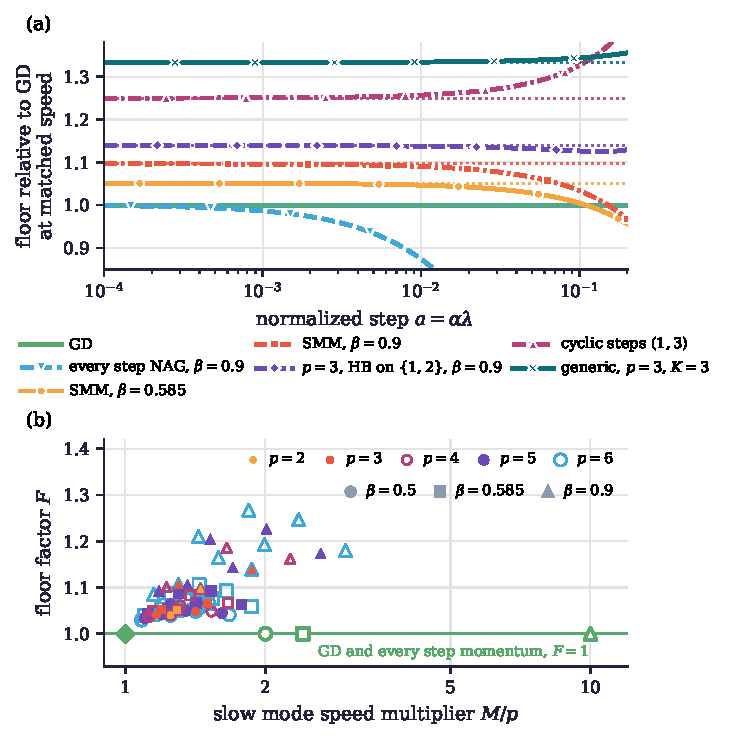
\includegraphics[width=\textwidth]{figures/ch7_gainweight.pdf}
\caption{The gain weight theorem. (a) Exact noise floor relative to gradient
descent at matched speed, from the periodic Lyapunov equation, against
$a=\alpha\lambda$, for six of the schedules of \cref{tab:ch7:gainweight} and for a period three schedule with three term memory and unrelated coefficients ($\mathcal F=1.333$); dotted lines are the limits $\mathcal F$. (b) The floor
factor $\mathcal F$ against the speed multiplier $M/p$ for all injection
subsets of periods $2$ to $6$ (larger markers for longer periods) and three values of $\beta$; only gradient
descent and every step momentum reach $\mathcal F=1$.}
\label{fig:ch7:gainweight}
\end{figure}

\section{The best period two ratio}\label{sec:ch7:pareto}

On quadratics \smmdet\ is the cyclic schedule with steps $h_1=\alpha$ and
$h_2=(1+\beta)\alpha$ (\cref{thm:smmquad}); in this section $h_1\le h_2$ denote absolute steps, not multiples of $\alpha$. Problem S3 asks which ratio
$r=h_2/h_1$ is best when both the deterministic rate and the noise floor\index{noise floor} matter.
For period two schedules both quantities depend on the ratio through a single
number,
\[
  G(r)=\frac{(1+r)^2}{4r}\ \geq1,
\]
and the tradeoff can be solved exactly.

\begin{proposition}[Rate and noise for period two steps]\label{prop:ch7:pareto}
Let the spectrum be $[\mu,L]$ with $\kappa=L/\mu$, and consider cyclic gradient
steps $h_1,h_2$ with ratio $r=h_2/h_1\ge1$.
\begin{enumerate}[label=(\roman*),leftmargin=2em]
\item The slow mode noise floor at matched speed is $N=2(h_1^2+h_2^2)/(h_1+h_2)^2
  =2-1/G(r)$.
\item For fixed $r$ with $G(r)\le G_{\mathrm{ch}}(\kappa)=2(\kappa+1)^2/(\kappa^2+6\kappa+1)$, the smallest possible worst case two step contraction over
  $[\mu,L]$ is
  \[
    R^*(r)=1-\frac{4\kappa\,G(r)}{(\kappa+1)^2},
  \]
  attained when the steps are scaled so that $h_1+h_2=4G(r)/(\mu+L)$.
  For $G(r)>G_{\mathrm{ch}}(\kappa)$ the smallest worst case contraction exceeds that of the Chebyshev ratio.
\item Consequently the Pareto frontier between rate and noise floor is
  $R=1-4\kappa/((2-N)(\kappa+1)^2)$ for $1\le N\le N_{\mathrm{ch}}(\kappa)$, where
  $N_{\mathrm{ch}}=(3\kappa^2+2\kappa+3)/(2(\kappa+1)^2)$ is the noise floor of
  the two step Chebyshev\index{Chebyshev step sizes} schedule, whose ratio tends to $(1+\sqrt2)^2=5.83$ and
  whose floor tends to $3/2$ as $\kappa\to\infty$.
\end{enumerate}
\end{proposition}

\begin{proof}
(i) is \eqref{eq:ch7:F} with $c=(h_1,h_2)$, and $2(h_1^2+h_2^2)/(h_1+h_2)^2
=2-4h_1h_2/(h_1+h_2)^2=2-1/G$. For (ii), the two step polynomial
$\Phi(\lambda)=(1-h_1\lambda)(1-h_2\lambda)$ satisfies $\Phi(0)=1$ and has minimum
$1-G$ at $\lambda_m=(h_1+h_2)/(2h_1h_2)$, so it can be written as
$\Phi(\lambda)=1-G+G(\lambda/\lambda_m-1)^2$. Its maximum over $[\mu,L]$ is at an
endpoint, and $\max\bigl((\mu/\lambda_m-1)^2,(L/\lambda_m-1)^2\bigr)$ is
minimized over $\lambda_m$ by $\lambda_m=(\mu+L)/2$, with value
$((\kappa-1)/(\kappa+1))^2$. Hence the endpoint maximum is at least
$1-G+G((\kappa-1)/(\kappa+1))^2=1-4\kappa G/(\kappa+1)^2$, with equality at
$\lambda_m=(\mu+L)/2$, i.e. $h_1+h_2=4G/(\mu+L)$.
At this scaling the interior minimum contributes $|1-G|=G-1$, and $G-1\le1-4\kappa G/(\kappa+1)^2$ exactly when $G\le G_{\mathrm{ch}}$, the two values being equal at the Chebyshev point $G=G_{\mathrm{ch}}$; since the endpoint bound holds for every scaling, this proves (ii) for such $G$.
For $G>G_{\mathrm{ch}}$ no scaling produces the two step Chebyshev polynomial~\cite{young1953,golub1961}, which is the unique minimizer of the worst case over $[\mu,L]$ among quadratic polynomials with value $1$ at $0$, so the worst case exceeds that of the Chebyshev ratio.
(iii) follows by eliminating $G=1/(2-N)$ for $G\le G_{\mathrm{ch}}$; beyond the Chebyshev point a larger ratio is worse than the Chebyshev ratio in both criteria.
\end{proof}

Every ratio between $1$ and the Chebyshev ratio $r_{\mathrm{ch}}(\kappa)$ is therefore on the frontier once its steps are scaled correctly, larger ratios being dominated by the Chebyshev ratio in both criteria, and the question becomes where on the frontier one wants to be.
The SMM ratio
$1+\beta$ gives $G=(2+\beta)^2/(4(1+\beta))=1.0540$ and $N=1.0512$: a $5.4$
percent gain in the rate exponent over optimally tuned gradient descent for a
$5.1$ percent rise in the noise floor. The Chebyshev ratio gains up to a factor
$2$ in the exponent but pays a floor up to $1.5$. The optimal scaling for the
SMM ratio is $\alpha L=4G\kappa/((2+\beta)(\kappa+1))$, which tends to
$(2+\beta)/(1+\beta)=1.631$; at the conventional $\alpha=1/L$ the method is not
on the frontier, and its per step factor at $\kappa=100$ is $0.9871$ against
$0.9791$ when optimally scaled. \Cref{fig:ch7:pareto} draws the frontier. The
SMM ratio coincides with the Chebyshev ratio only at $\kappa_0=1.94$; for
larger $\kappa$ it sits close to the gradient descent end of the frontier,
which is the noise conservative end.

\begin{figure}[tbp]
\centering
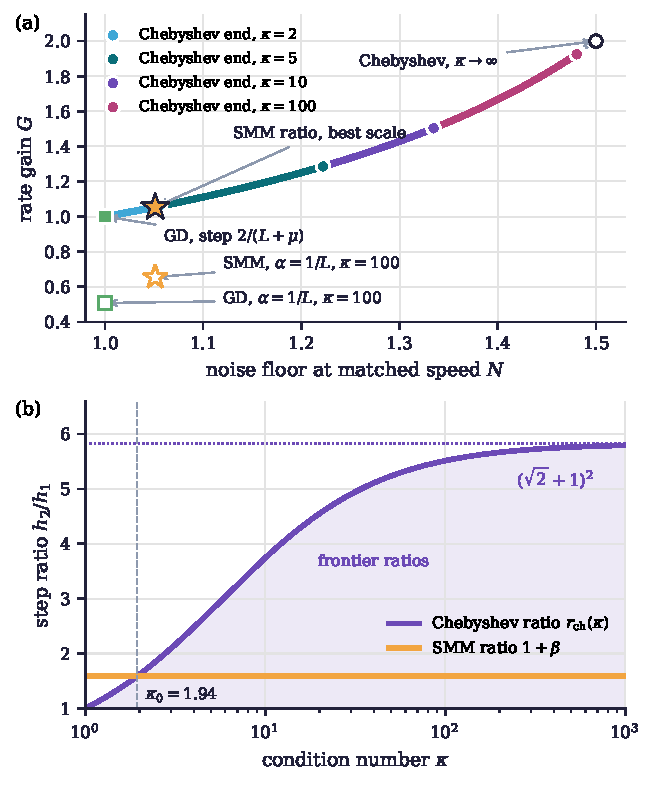
\includegraphics[width=\textwidth]{figures/ch7_pareto.pdf}
\caption{(a) The rate gain $G$ against the noise floor $N$ at matched speed for period two schedules. By \cref{prop:ch7:pareto}(i) all frontiers lie on the curve $G=1/(2-N)$ and differ only in where they end, at the Chebyshev schedule for each $\kappa$. The star is the SMM ratio at its best scale, the open markers SMM and gradient descent at $\alpha=1/L$ and $\kappa=100$, and the filled square gradient descent at step $2/(L+\mu)$. The frontier ends for $\kappa=2,5,10,100$ lie in that order along the curve: the first under the star, the others at the dots. (b) The Chebyshev ratio $r_{\mathrm{ch}}(\kappa)$, rising to $(1+\sqrt2)^2$, and the SMM ratio $1+\beta$; they cross at $\kappa_0=1.94$.}
\label{fig:ch7:pareto}
\end{figure}

\section{Multiplicative noise}\label{sec:ch7:multiplicative}

Additive noise is the simplest model. In least squares, and more generally in
stochastic gradient methods with sampled data, the noise also multiplies the
error: the sampled curvature fluctuates. Problem S2 asks whether the
conclusions survive. Consider on one eigendirection the oracle
\[
  g(y)=(\lambda+\eta_t)\,e_y+\xi_t,
\]
with $\eta_t,\xi_t$ independent of the past, mean zero, uncorrelated with each
other, $\Var(\alpha\eta_t)=\omega^2$ and $\Var\xi_t=\sigma^2$. Two scalings are
natural: the least squares scaling $\omega^2=\vartheta a^2$, in which the
relative curvature noise\index{multiplicative noise} $\vartheta=\Var(x^2)/(\E x^2)^2$ is fixed ($\vartheta=2$
for a Gaussian regressor), and the diffusive scaling $\omega^2=\epsilon a$.

\begin{proposition}[Multiplicative noise]\label{prop:ch7:mult}
For \smmdet\ the second moments obey a closed linear recursion: with
$\nu_1=(1-a)^2+\omega^2$ and $\nu_2=(1-(1+\beta)a)^2+(1+\beta)^2\omega^2$,
the stationary second moment at even times is
$\alpha^2\sigma^2(\nu_1(1+\beta)^2+1)/(1-\nu_1\nu_2)$, finite if and only
if $\nu_1\nu_2<1$. As $a\to0$:
\begin{enumerate}[label=(\roman*),leftmargin=2em]
\item under the least squares scaling the slow mode ratio to gradient descent is
  unchanged, $(2+2\beta+\beta^2)/(2+\beta)$, for every $\vartheta$;
\item under the diffusive scaling, for any linear periodic method that is stable at $a=0$ and has $M>0$, with
  gains $c_i$, $a\,\E e^2\to\alpha^2\sigma^2\sum_ic_i^2/(2M-\epsilon\sum_ic_i^2)$,
  so the method is mean square stable for small $a$ exactly when
  $\epsilon<\epsilon^*=2M/\sum_ic_i^2$.
\end{enumerate}
\end{proposition}

\begin{proof}
For \smmdet\ the two step recursion of \cref{thm:smmvar} holds with each factor
$(1-ha)$ replaced by $(1-h(a+\alpha\eta))$; squaring and taking expectations,
the cross terms vanish by independence and the factors $\nu_1,\nu_2$
appear, which gives the closed form and the stability condition. Statement (i)
follows because $\omega^2=\vartheta a^2$ changes $\nu_1,\nu_2$ only at order
$a^2$, which does not affect the leading term of $1-\nu_1\nu_2$. For (ii),
repeat the slow coordinate argument of \cref{thm:ch7:gainweight}: the
multiplicative noise contributes to $s$ a term $-\alpha\sum_ic_i\eta_{t+i}s$ per
period, of variance $\epsilon a\sum_ic_i^2\,s^2$, so the stationary second
moment satisfies $\E s^2=(1-2Ma+\epsilon a\sum c_i^2)\E s^2+\alpha^2\sigma^2\sum
c_i^2+o(a)\E s^2$, which gives the stated limit and threshold.
\end{proof}

The threshold $\epsilon^*=2M/\sum c_i^2$ is a clean measure of robustness to
curvature noise. It is $2$ for gradient descent, $2(1-\beta)$ for every step
momentum\index{momentum}, $0.830$ at $\beta=\beta_0=\lt-1$ and $0.2$ at $\beta=0.9$, and
$2(2+\beta)/((1+\beta)^2+1)$ for \smmdet, which is $1.472$ at $\beta_0$ and
$1.258$ at $\beta=0.9$ and never falls below $6/5$. So under curvature noise the
parity schedule is markedly more robust than every step momentum, by a factor
that grows without bound as $\beta\to1$.
At matched slow mode speed the comparison changes, as it did for the variance: gradient descent with step $(M/p)\alpha$ has $\epsilon^*=2p/M$, and the ratio of the two thresholds is $M^2/(p\sum_ic_i^2)=1/\mathcal F\le1$.
Away from the slow mode the picture is
more nuanced. The uniform bound $5/3$ does not survive large multiplicative
noise at large $a$: at $\beta=\beta_0$ \smmdet\ remains mean square stable at
$a=1$ only for $\vartheta<0.566$, and above that it is not mean square stable at $a=1$, where gradient descent still is for $\vartheta<1$; but every step Nesterov\index{Nesterov acceleration} loses
stability earlier at every $\vartheta$ we examined (\cref{fig:ch7:multiplicative},
script \texttt{ch7\_multiplicative.py}, with Monte Carlo checks agreeing with the
closed forms to three digits).

\begin{figure}[tbp]
\centering
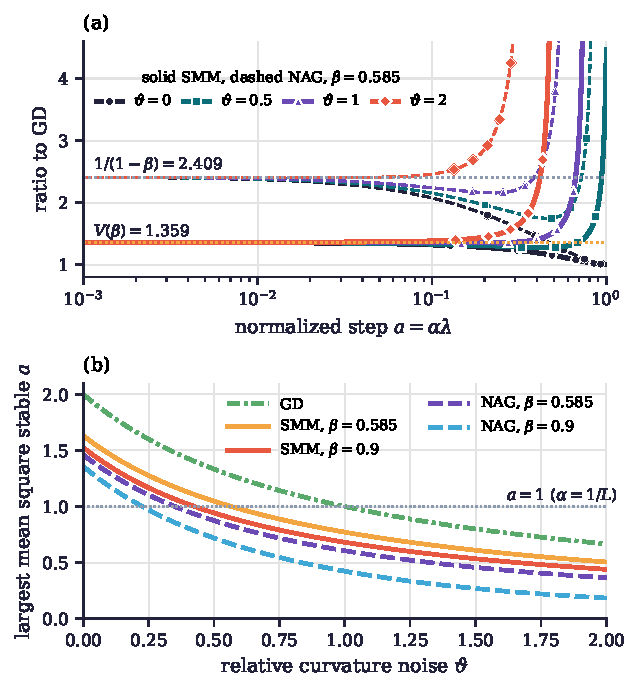
\includegraphics[width=\textwidth]{figures/ch7_multiplicative.pdf}
\caption{Multiplicative noise under the least squares scaling. (a) Stationary
second moment relative to gradient descent against $a$, for \smmdet\ (solid)
and every step Nesterov (dashed) at $\beta=0.585$ and several $\vartheta$; the
slow mode limits $V(\beta)=1.359$ and $1/(1-\beta)=2.409$ are marked. (b) The
largest mean square stable $a$ as a function of $\vartheta$; \smmdet\ is stable
on a larger range than every step Nesterov at the same $\beta$.}
\label{fig:ch7:multiplicative}
\end{figure}

\section{The experiments}\label{sec:ch7:experiments}

We now describe experiments with SMM and then reconcile them with the exact theory in \cref{sec:ch7:reconcile}. The experiments were designed before that theory was available. The numbers and figures below come from a rerun for this book: the script \texttt{ch7\_experiments.py} runs the experiments, and the scripts \texttt{ch7\_experiments\_fig.py} and \texttt{ch7\_noisefig.py} draw the figures.

\subsection{Setup and baselines}

\smmdet\ and, where indicated, \smmstate\ (\cref{alg:smmdet,alg:smmstate}) were
compared with gradient descent at step $1/L$; with heavy ball\index{heavy ball} and Nesterov\index{Nesterov acceleration} at
their textbook strongly convex tunings~\cite{polyak1987,nesterov2004}, which
need $\mu$ (heavy ball with $\alpha=4/(\sqrt L+\sqrt\mu)^2$ and
$\beta=\bigl((\sqrt L-\sqrt\mu)/(\sqrt L+\sqrt\mu)\bigr)^2$, Nesterov with
$\alpha=1/L$ and $\beta=(\sqrt L-\sqrt\mu)/(\sqrt L+\sqrt\mu)$); and with fixed
momentum\index{momentum} heavy ball and Nesterov at the four candidates
$\beta\in\{0.5,0.585,0.667,0.9\}$ of \cref{tab:ch6:candidates}. The fixed
momentum row at $\beta=0.585$ is the every step analogue of \smmdet\ and
isolates the parity schedule. Adam~\cite{kingma2015} at its defaults
($\beta_1=0.9$, $\beta_2=0.999$, $\epsilon=10^{-8}$, step $1/L$) served as a
reference from a different family. Every method received $L$.
Fixed momentum Nesterov is the update $y_t=x_t+\beta(x_t-x_{t-1})$, $x_{t+1}=y_t-\alpha\nabla f(y_t)$ at every step, and fixed heavy ball the update of \cref{sec:ch7:ar2}, both with $\alpha=1/L$; the frequency ablation adds injection at random steps, each step injecting independently with probability $\tfrac12$. \smmstate\ runs \cref{alg:smmstate} with $\rho_{\mathrm{thr}}=0.356$, reference value $f_{\mathrm{ref}}=f^\ast$, the minimum of the objective, and $\epsilon=10^{-12}$.

The test problems were random quadratics $f(x)=\tfrac12x^\top Ax$ in dimension $d=25$, with eigenvalues geometrically spaced in $[1,\kappa]$, a random orthogonal eigenbasis and $x_0$ drawn from $N(0,I)$; and $\ell_2$ regularized logistic regression on the Breast Cancer Wisconsin data~\cite{wolberg1995} ($n=569$ samples, $30$ standardized features, no intercept, penalty $0.05$), with initial weights drawn from $N(0,0.1^2I)$; there $\mu=0.05$ and $L=\lambda_{\max}(X^\top X/n)/4+0.05=3.370$ for the $n\times30$ data matrix $X$, so that $\kappa=L/\mu\approx67.4$. The count of a run is the first iteration at which the objective gap falls below the tolerance, and a run that has not reached the tolerance within the horizon $T$ counts as $T+1$. Means and standard errors are over $R$ seeded replicates: $R=20$ for the quadratic and logistic experiments, $R=30$ for the noise sweep and the minibatch test.

\subsection{Quadratic condition number sweep and frequency ablation}

\Cref{fig:ch7:ksweep} reports the mean number of iterations to reach an objective gap below $10^{-4}$ for $\kappa\in\{2,5,10,25,50,100\}$, with horizon $T=300$. At $\kappa=2$, \smmdet\ is the fastest method tested, with $4.85$ iterations on average. At $\kappa=5$ only every step Nesterov\index{Nesterov acceleration} at $\beta=0.5$ and at $\beta=0.585$ is clearly faster ($11.85$ and $12.6$ iterations against $15.95$); Nesterov at $\beta=0.667$ ties with \smmdet, and every step heavy ball\index{heavy ball} at these coefficients is slower. For $\kappa\ge10$ every step heavy ball and Nesterov at $\beta\in\{0.585,0.667\}$ beat it, by factors from about $1.1$ to $2.0$ at $\kappa=10$ and from $2.1$ to $2.9$ at $\kappa=25$. At $\kappa=50$ the coefficient $0.667$ is fastest in both forms, and only at $\kappa=100$ is fixed Nesterov at $\beta=0.9$ fastest. The nearly flat stretches of the fixed heavy ball curves reflect underdamping: when every normalized step exceeds $(1-\sqrt\beta)^2$, which holds for $\kappa<(1-\sqrt\beta)^{-2}$ (about $12$, $18$, $30$ and $380$ for the four candidates), both characteristic roots have modulus $\sqrt\beta$ whatever $a$, so the iteration count is set by $\beta$ rather than by the conditioning.

\begin{figure}[tbp]
  \centering
  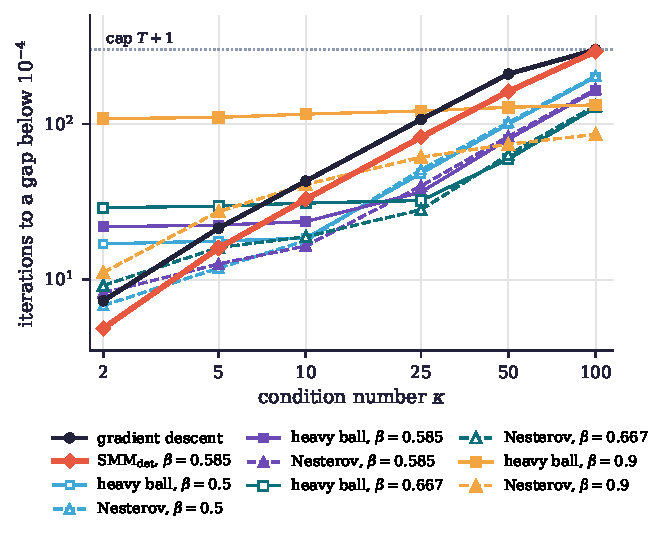
\includegraphics[width=\textwidth]{figures/ch7_ksweep.pdf}
  \caption{Fixed momentum baselines on random quadratics ($d=25$, $R=20$,
  $T=300$): mean iterations to an objective gap below $10^{-4}$ against the
  condition number. Heavy ball (squares, solid) and Nesterov (triangles,
  dashed) at the four candidate coefficients, gradient descent, and \smmdet.
  A run that has not reached the tolerance by $T$ counts as $T+1=301$ (dotted line); at $\kappa=100$ this cap censors $19$ of the $20$ gradient descent runs and $14$ of the $20$ \smmdet\ runs.}
  \label{fig:ch7:ksweep}
\end{figure}

\Cref{fig:ch7:ablation} isolates the schedule at $\beta=0.585$: injection at every step, at odd steps (\smmdet), at random steps with probability $\tfrac12$, and never. Without noise, parity does not help. Every step injection needs $16.45$ iterations at $\kappa=10$ against $32.85$ for parity, a ratio of $2.00$, and $167$ against $293$ at $\kappa=100$; there $14$ of the $20$ parity runs reach the horizon, so the parity count is censored, and continued to convergence (the script runs every instance for $3000$ steps) the parity schedule needs $318$ iterations, a ratio of $1.90$. Random injection lies between the two, closer to parity for $\kappa\ge10$. Only at $\kappa=2$, where all normalized steps are large and the period two polynomial $\rho(a)$ is small, does parity win. The ratios $2.00$ and $1.90$ are close to the slow mode prediction $m_{\mathrm{NAG}}/m_{\mathrm{SMM}}=1.86$ of \cref{cor:ch6:slow} and the discussion following it; \cref{chap:smm} makes the same check with more replicates.

\begin{figure}[tbp]
  \centering
  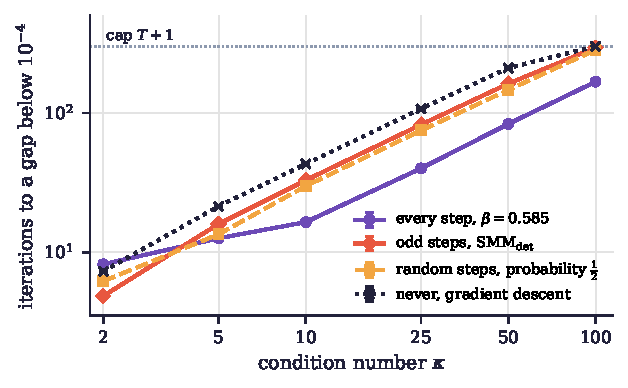
\includegraphics[width=\textwidth]{figures/ch7_ablation.pdf}
  \caption{Frequency ablation on random quadratics at fixed $\beta=0.585$
  ($d=25$, $R=20$, $T=300$): injection at every step, at odd steps (\smmdet),
  at random steps with probability $\tfrac12$, and never (gradient descent).
  Bars are standard errors. A run that has not reached the tolerance by $T$ counts as $301$ (dotted line), which censors most parity and gradient descent runs and half of the random injection runs at $\kappa=100$.}
  \label{fig:ch7:ablation}
\end{figure}

\subsection{Noise robustness}

The central experiment adds Gaussian noise of standard deviation $\sigma\in\{0,\allowbreak0.05,\allowbreak0.10,\allowbreak0.20,\allowbreak0.40\}$ to the gradients of random quadratics with $\kappa=25$, with the same noise draws for every method, and records the objective gap after $T=300$ steps (\cref{fig:ch7:noise,tab:noise}). At every positive noise level \smmdet\ has the lowest final gap among the inertial methods: at $\sigma=0.1$, $3.7\times10^{-3}$ against $5.0\times10^{-3}$ for every step Nesterov momentum\index{momentum} at the same $\beta$ and $1.1\times10^{-2}$ at $\beta=0.9$. Across the sweep every step Nesterov at $\beta=0.585$ is $29$ to $36$ percent worse than \smmdet, and $\beta=0.9$ about $2.5$ to $3$ times worse; heavy ball at the same coefficients is worse still. Gradient descent has the lowest gap of all at each positive $\sigma$, and \smmdet\ stays within $27$ percent of it.

\begin{figure}[tbp]
  \centering
  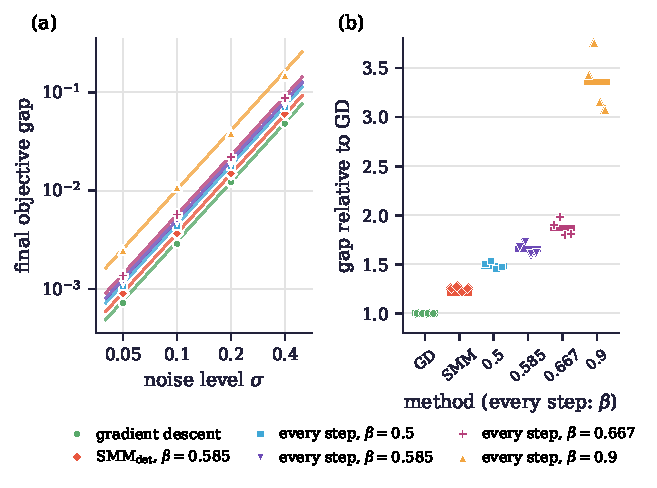
\includegraphics[width=\textwidth]{figures/ch7_noise.pdf}
  \caption{The noise robustness experiment of \cref{tab:noise}. (a) Final
  objective gap after $T=300$ steps against the noise level (points), with the
  stationary predictions of \eqref{eq:ch7:gd}, \cref{thm:smmvar} and \cref{prop:ch7:nag} summed
  over the spectrum (lines). (b) The gap relative to gradient descent for
  each method at the four positive noise levels (points), with the predicted ratios marked (bars). The every step rows use the Nesterov form.}
  \label{fig:ch7:noise}
\end{figure}

\begin{table}[tbp]
\centering
\caption{Noise robustness on random quadratics with $\kappa=25$ ($d=25$,
$T=300$, $R=30$): final objective gap, lower is better. A dagger marks the
lowest gap among inertial methods at each positive noise level; gradient
descent, which has no momentum, is lower still. ``every, $\beta$'' denotes
Nesterov momentum $\beta$ injected at every step, and ``HB, $\beta$'' heavy ball.}
\label{tab:noise}
\footnotesize
\setlength{\tabcolsep}{2.2pt}
\begin{tabular}{lccccc}
\toprule
Method & $\sigma=0$ & $0.05$ & $0.10$ & $0.20$ & $0.40$\\
\midrule
GD & $1.8\times10^{-11}$ & $7.2\times10^{-4}$ & $2.9\times10^{-3}$ & $1.2\times10^{-2}$ & $4.8\times10^{-2}$\\
every, $0.5$ & ${\approx}\,0$ & $1.1\times10^{-3}$ & $4.4\times10^{-3}$ & $1.8\times10^{-2}$ & $7.1\times10^{-2}$\\
every, $0.585$ & ${\approx}\,0$ & $1.2\times10^{-3}$ & $5.0\times10^{-3}$ & $2.0\times10^{-2}$ & $7.8\times10^{-2}$\\
\smmdet, parity & $1.1\times10^{-14}$ & $9.0\times10^{-4}\,^\dagger$ & $3.7\times10^{-3}\,^\dagger$ & $1.5\times10^{-2}\,^\dagger$ & $6.0\times10^{-2}\,^\dagger$\\
every, $0.667$ & ${\approx}\,0$ & $1.4\times10^{-3}$ & $5.7\times10^{-3}$ & $2.2\times10^{-2}$ & $8.7\times10^{-2}$\\
every, $0.9$ & ${\approx}\,0$ & $2.5\times10^{-3}$ & $1.1\times10^{-2}$ & $3.8\times10^{-2}$ & $1.5\times10^{-1}$\\
HB, $0.585$ & ${\approx}\,0$ & $1.5\times10^{-3}$ & $6.7\times10^{-3}$ & $2.6\times10^{-2}$ & $1.1\times10^{-1}$\\
HB, $0.9$ & $1.2\times10^{-12}$ & $6.3\times10^{-3}$ & $2.8\times10^{-2}$ & $1.1\times10^{-1}$ & $3.9\times10^{-1}$\\
\bottomrule
\end{tabular}
\end{table}

\subsection{Logistic regression and Adam}

On the regularized logistic regression (\cref{tab:ch7:logistic}, horizon $T=600$), fixed momentum\index{momentum} $\beta=0.667$ is fastest in both forms, with about $41$ iterations to a gap below $10^{-4}$; the Collatz coefficient at every step needs about $52$, \smmdet\ about $100$ and gradient descent $129$. Without noise, every step injection at a moderate fixed $\beta$ is the better choice. \Cref{fig:ch7:logistic} adds the tuned methods, which use $\mu$ and reach machine precision far sooner ($19.3$ and $29.0$ iterations to the tolerance for heavy ball and Nesterov), and \smmstate, whose rule fires at almost every step on this problem ($599.5$ of the $600$ steps on average), so that it follows every step Nesterov at $\beta=0.585$, with $53.0$ iterations. Adam, with $75.9$ iterations, lies between fixed Nesterov\index{Nesterov acceleration} at $\beta=0.9$ ($50.3$) and \smmdet. Adam keeps two moment vectors per coordinate where SMM, heavy ball\index{heavy ball} and Nesterov keep one extra vector; it needs neither $\mu$ nor a tuned coefficient, but on this problem every fixed momentum method except heavy ball at $\beta=0.9$ is faster.

\begin{table}[tbp]
\centering
\caption{Logistic regression on the Breast Cancer Wisconsin data (penalty $0.05$,
$\kappa\approx67.4$, $T=600$, $R=20$): iterations to a gap below $10^{-4}$ (mean
and standard error), observed speedup over gradient descent, and the slow mode
prediction of \cref{sec:ch7:reconcile}. An asterisk marks methods underdamped in
the slowest mode.}
\label{tab:ch7:logistic}
\begin{tabular}{lccc}
\toprule
Method & Iterations & Speedup & Predicted\\
\midrule
GD & $128.8\pm1.5$ & $1$ & $1$\\
HB, $\beta=0.5$ & $63.1\pm0.7$ & $2.04$ & $2.08$\\
HB, $\beta=0.585$ & $51.6\pm0.6$ & $2.50$ & $2.58$\\
HB, $\beta=0.667$ & $40.3\pm0.4$ & $3.20$ & $3.41$\\
HB, $\beta=0.9$ & $77.0\pm1.0$ & $1.67$ & $3.52^{*}$\\
NAG, $\beta=0.5$ & $64.1\pm0.7$ & $2.01$ & $2.05$\\
NAG, $\beta=0.585$ & $52.8\pm0.6$ & $2.44$ & $2.52$\\
NAG, $\beta=0.667$ & $41.9\pm0.5$ & $3.08$ & $3.28$\\
NAG, $\beta=0.9$ & $50.3\pm0.3$ & $2.56$ & $4.02^{*}$\\
\smmdet, $\beta=0.585$ & $99.7\pm1.2$ & $1.29$ & $1.30$\\
\bottomrule
\end{tabular}
\end{table}

\begin{figure}[tbp]
  \centering
  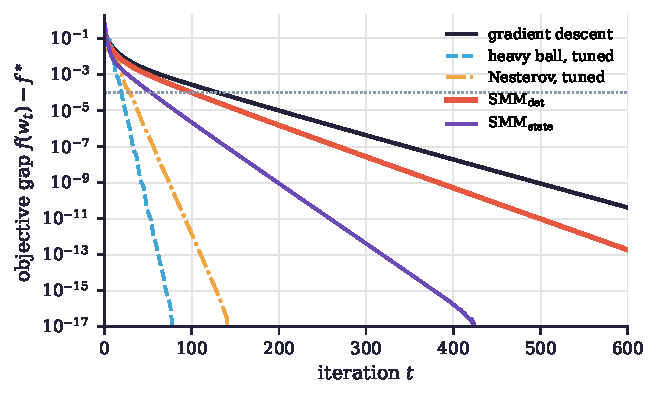
\includegraphics[width=\textwidth]{figures/ch7_logistic.pdf}
  \caption{Logistic regression (penalty $0.05$, $\kappa\approx67$, $T=600$, mean
  of $R=20$ runs): objective gap against iteration for gradient descent, tuned
  heavy ball and Nesterov, \smmdet\ and \smmstate; the dotted line is the tolerance $10^{-4}$.
  \smmstate\ injects at almost every step here and follows every step Nesterov at $\beta=0.585$.}
  \label{fig:ch7:logistic}
\end{figure}

\subsection{Minibatch stochastic gradients}

A more realistic test replaces the full logistic gradient by minibatch gradients with $|B|\in\{16,64,256\}$, the batches drawn without replacement and shared by all methods, keeping the step $1/L$ (\cref{tab:ch7:sgd,fig:ch7:sgd}). At $|B|=16$ every method that injects at every step, including tuned Nesterov\index{Nesterov acceleration}, reaches the tolerance $10^{-3}$ late or not at all: tuned Nesterov and Nesterov at $\beta=0.9$ in none of the $30$ runs, Nesterov at $\beta=0.585$ after $273$ iterations on average, with $2$ runs that never do. \smmdet\ is the only inertial method that reaches it reliably, in $135$ iterations, and gradient descent, with $118$, is faster still. As the batch grows the deterministic ranking returns: at $|B|=256$ tuned Nesterov is fastest with $21$ iterations. Among the every step Nesterov variants the default $\beta=0.9$ is never faster than the others: at $|B|=16$ it ties with tuned Nesterov, neither reaching the tolerance, and at $|B|=64$ and $256$ it is the slowest of the three.

\begin{table}[tbp]
\centering
\caption{Minibatch stochastic gradients on the logistic regression: iterations
to a gap below $10^{-3}$ (mean and standard error, $T=600$, $R=30$; a run that does not reach the tolerance within $T$ counts as $601$). A dagger
marks the best inertial method at each batch size; ``cap'' marks entries in which no run reached the tolerance.}
\label{tab:ch7:sgd}
\begin{tabular}{lccc}
\toprule
Method & $|B|=16$ & $|B|=64$ & $|B|=256$\\
\midrule
GD & $118.2\pm6.3$ & $77.7\pm1.5$ & $67.6\pm1.1$\\
NAG, tuned & $601\pm0$ (cap) & $36.5\pm2.3\,^\dagger$ & $21.2\pm0.2\,^\dagger$\\
NAG, $\beta=0.585$ & $272.7\pm30.7$ & $40.6\pm1.3$ & $29.3\pm0.5$\\
NAG, $\beta=0.9$ & $601\pm0$ (cap) & $113.5\pm14.7$ & $36.5\pm0.8$\\
\smmdet, $\beta=0.585$ & $135.2\pm11.2\,^\dagger$ & $62.7\pm1.7$ & $53.1\pm0.9$\\
\bottomrule
\end{tabular}
\end{table}

\begin{figure}[tbp]
  \centering
  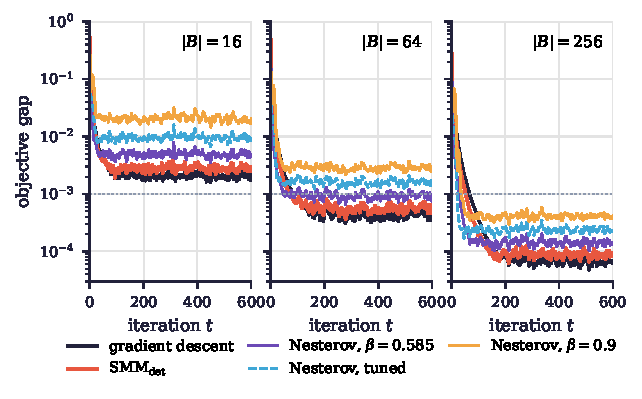
\includegraphics[width=\textwidth]{figures/ch7_sgd.pdf}
  \caption{Minibatch stochastic gradients on the logistic regression ($T=600$,
  mean of $R=30$ runs; the dotted line is the tolerance $10^{-3}$). In every panel the plateaus are ordered from gradient
  descent (lowest) through \smmdet, Nesterov at $\beta=0.585$ and tuned Nesterov
  to Nesterov at $\beta=0.9$ (highest).}
  \label{fig:ch7:sgd}
\end{figure}

In summary, read on their own, the experiments say the following: without noise, every step Nesterov momentum beats \smmdet\ at the same coefficient for $\kappa\ge5$, and every step heavy ball for $\kappa\ge10$; with noise, \smmdet\ has the lowest final gap among inertial methods and copes best with the smallest minibatch; and $0.585$ is a reasonable default among fixed momenta but not a universally optimal one, and nothing in the theory of this chapter singles it out.

\section{Reconciling the experiments with the exact theory}\label{sec:ch7:reconcile}

\paragraph{The noise floors.} The $\kappa=25$ experiment has $\alpha=1/25$ and
normalized steps $a_j=\lambda_j/25\in[0.04,1]$. After $T=300$ steps the
deterministic transient has decayed by at least $0.96^{300}<10^{-5}$, so by
\eqref{eq:ch7:gap} the final gap is essentially
$\tfrac12\sum_{j}\lambda_jV(a_j)$, with $V$ the exact stationary variance of the
method. For gradient descent this sum is $0.3055\,\sigma^2$, that is
$7.6\times10^{-4}$, $3.05\times10^{-3}$, $1.22\times10^{-2}$ and
$4.89\times10^{-2}$ at the four noise levels, against the measured
$7.2\times10^{-4}$, $2.9\times10^{-3}$, $1.22\times10^{-2}$ and $4.8\times10^{-2}$.
\Cref{tab:ch7:reconcile} does the same for the ratios to gradient descent.
The every step rows of \cref{tab:noise} use the Nesterov\index{Nesterov acceleration} form of every step momentum\index{momentum}, and its predictions match the data closely at all four coefficients; so do the much larger heavy ball\index{heavy ball} predictions for the two heavy ball rows.
The predicted ratio of every step Nesterov at $\beta=0.585$ to \smmdet\ is $1.65/1.21=1.36$, matching the observed $29$ to $36$ percent, and the predicted excess of \smmdet\ over gradient descent is $21$ percent, against the observed $22$ to $27$ percent.

\begin{table}[tbp]
\centering
\caption{Final gap relative to gradient descent in the $\kappa=25$ noise
experiment: prediction from the exact stationary variances summed over the
spectrum, and the range of measured ratios over the four positive noise levels
of \cref{tab:noise}.}
\label{tab:ch7:reconcile}
\begin{tabular}{lcc}
\toprule
Method & Predicted & Measured\\
\midrule
\smmdet, $\beta=0.585$ & $1.21$ & $1.22$ to $1.27$\\
NAG, $\beta=0.5$ & $1.49$ & $1.46$ to $1.54$\\
NAG, $\beta=0.585$ & $1.65$ & $1.61$ to $1.73$\\
NAG, $\beta=0.667$ & $1.87$ & $1.80$ to $1.98$\\
NAG, $\beta=0.9$ & $3.36$ & $3.07$ to $3.76$\\
HB, $\beta=0.585$ & $2.21$ & $2.14$ to $2.31$\\
HB, $\beta=0.9$ & $8.96$ & $8.02$ to $9.86$\\
\bottomrule
\end{tabular}
\end{table}

\paragraph{Why gradient descent wins the noise table.} That gradient descent has
the lowest final gap at every positive $\sigma$ is forced by the theory.
At a fixed step every inertial method considered has stationary variance at least that of gradient descent on every eigendirection with $a\le1$: for \smmdet\ by \cref{prop:ch7:uniform}; for Nesterov because $V_{\mathrm{NAG}}-V_{\mathrm{GD}}=2\beta(1+\beta)(1-a)^2\alpha^2\sigma^2/\bigl(a(2-a)(1-\beta+a\beta)(2(1+\beta)-a(1+2\beta))\bigr)\ge0$, an identity checked by \texttt{ch7\_extra.py}; and for heavy ball because its ratio $(1+\beta)(2-a)/\bigl((1-\beta)(2(1+\beta)-a)\bigr)$ is at least $1$ whenever $a\le1+\beta$.
The dagger in \cref{tab:noise} is therefore to be read with the
gradient descent row: \smmdet\ gives up little of the quietness of gradient
descent while being faster than it without noise, and every step momentum gives
up much more.

\paragraph{The minibatch test.} The noise of a minibatch gradient is neither
additive nor isotropic, but the plateaus of \cref{fig:ch7:sgd} are ordered exactly as the
slow mode amplifications: gradient descent ($1$), \smmdet\ ($1.36$), Nesterov at
$\beta=0.585$ ($2.41$), tuned Nesterov, whose coefficient at $\kappa=67.4$ is
$0.783$ with $1/(1-\beta)=4.60$, and Nesterov at $\beta=0.9$ ($10$). The
iteration counts mix this ordering with speed (\cref{rem:ch7:budget}). At
$|B|=16$ the mean plateaus of all methods lie near or above $10^{-3}$, so the
count is a first passage time of a fluctuating gap below a level close to the
floor; the lower the floor, the sooner the crossing, which favours gradient
descent and \smmdet. At $|B|=256$ all floors lie well below the tolerance and
speed decides.

\paragraph{The deterministic speedups.} In the slowest mode of the logistic
regression, $a=1/67.4$, the predicted speedup over gradient descent is
$\log r/\log(1-a)$, where $r$ is the per step factor of the method: the spectral
radius of its companion matrix, or $|\rho(a)|^{1/2}$ for \smmdet.
For \smmdet\ the prediction, $1.296$, agrees within $0.3$ percent with the observed ratio of the mean counts, $128.80/99.65=1.293$; for the overdamped heavy ball and Nesterov runs, $\beta\le0.667$, prediction and observation agree within seven percent, the prediction always
slightly optimistic, as expected of a count that includes the initial
transient. Only the underdamped runs at $\beta=0.9$ deviate, since their
oscillatory convergence is not governed by the asymptotic rate alone.

In short, the exact theory confirms the qualitative findings, explains their magnitudes, and adjusts one reading: in the slow modes SMM is not more efficient than gradient descent under noise, although over the whole spectrum of the $\kappa=25$ experiment its floor, $1.21$ times that of gradient descent at the same step, is below the $1.42$ of gradient descent run at the same slow mode speed; it is much quieter than every step momentum at the same $\beta$, and its noise behaviour is almost insensitive to $\beta$.

\section{Practical guidance and limitations}\label{sec:ch7:guidance}

If gradients are exact and $\mu$ is available, a tuned accelerated method is
the right tool; SMM is not accelerated. If gradients are exact and $\mu$ is
unknown, every step momentum\index{momentum} at a moderate fixed coefficient such as $0.585$ or
$0.667$ is faster than SMM by a factor near $m_{\mathrm{NAG}}/m_{\mathrm{SMM}}$.
If gradients are noisy at an unknown level, \smmdet\ is a safe default: its
floor is within $5/3$ of that of gradient descent at the same step for every
$\beta<1$ and on every eigendirection, it is stable at step $1/L$ for every
$\beta<1$, and at the Collatz coefficient it is about $29$ percent faster than
gradient descent in the slow modes; if only the floor at a given slow mode speed matters, gradient descent with a slightly longer step is slightly better in the slow eigendirections but worse over the whole spectrum ($1.42$ against $1.21$ in the $\kappa=25$ experiment).
If per coordinate preconditioning is affordable, Adam is an alternative that needs no $\mu$, although in the logistic experiment it was slower than every step momentum at a moderate coefficient. Iterate
averaging~\cite{polyak1992} or a decreasing step lowers the floor of any of
these methods; our comparisons are for a constant step.

The exact noise theory covers quadratics, with additive noise independent across iterations (\cref{thm:smmvar,thm:ch7:gainweight}) and, for \smmdet, multiplicative noise (\cref{prop:ch7:mult}).
For nonquadratic objectives the noiseless theory is \cref{prop:ch6:defect} together with two results of \cref{chap:difference}, which follows this chapter: \smmdet\ decreases $f$ on alternate iterates for every $L$ smooth $f$ (\cref{prop:ch5b:monotone}), and it converges linearly, at an explicit rate in terms of $\mu$ and $L$, for every $\mu$ strongly convex and $L$ smooth $f$ (\cref{thm:ch5b:rate}).
Under noise we have no theory beyond quadratics, and for minibatch noise only the qualitative agreement above.
The experiments are small, in dimensions $25$ and $30$.
For \smmstate\ the only theory is the stability on quadratics of every switching rule, which \cref{cor:ch5b:anyswitch} proves conditionally on \cref{conj:ch5b:transient}.
Nothing here bears on the Collatz conjecture\index{Collatz conjecture}: the arithmetic
supplied a number and a pattern, and what they do as an optimizer is ordinary
linear algebra.

\section*{Notes}

The AR(2) analysis of heavy ball\index{heavy ball} under additive noise is classical and appears
in many forms; Polyak\index{Polyak, B. T.}'s book~\cite{polyak1987} treats momentum\index{momentum} on quadratics in
detail, and the time series background is in Brockwell and
Davis~\cite{brockwell1991}. That constant momentum does not improve the
efficiency of stochastic gradient descent in the small step regime, because the
effective step and the noise both scale by $1/(1-\beta)$, was established in
generality by Yuan\index{Yuan, K.}, Ying\index{Ying, B.} and Sayed\index{Sayed, A. H.}~\cite{yuan2016}; Kidambi\index{Kidambi, R.}, Netrapalli\index{Netrapalli, P.}, Jain\index{Jain, P.}
and Kakade\index{Kakade, S. M.}~\cite{kidambi2018} showed that heavy ball and Nesterov\index{Nesterov acceleration} with
stochastic gradients need not improve on stochastic gradient descent even on
least squares. \Cref{prop:ch7:matched} is the period two analogue for SMM.

\Cref{thm:smmvar}, \cref{prop:ch7:bound}, \cref{prop:ch7:uniform} and
\cref{prop:ch7:matched} are new in this book.
The gain weight theorem (\cref{thm:ch7:gainweight}), \cref{prop:ch7:pareto} and \cref{prop:ch7:mult} are also proved here; in the equal gain case the gain weight theorem recovers, in the slow mode, the equivalence of Yuan, Ying and Sayed~\cite{yuan2016}.
The experiments of \cref{sec:ch7:experiments}, the reconciliation of \cref{sec:ch7:reconcile}, the predicted columns of \cref{tab:ch7:logistic,tab:ch7:reconcile}, and the corresponding computations were done for this book with the scripts listed in Appendix~\ref{app:code}.
Iterate averaging in stochastic approximation is due independently to Ruppert\index{Ruppert, D.}~\cite{ruppert1988} and to Polyak~\cite{polyak1990}; Polyak and Juditsky\index{Juditsky, A. B.}~\cite{polyak1992} give the standard analysis.

\section*{Exercises}

\begin{exercise}
Show that the stationary variance of the AR(2) process of \cref{lem:ch7:ar2} can
be written as $s^2(1-a_2)/\bigl((1+a_2)(1-a_1-a_2)(1+a_1-a_2)\bigr)$, and use this
form to rederive \cref{prop:ch7:hb,prop:ch7:nag} in one line each. Compute
$\gamma_1/\gamma_0$ for heavy ball\index{heavy ball} in the slow mode limit and interpret it.
\end{exercise}

\begin{exercise}
Let $p\ge1$ and consider noisy gradient descent on a scalar quadratic with the
periodic steps $h_1\alpha,\dots,h_p\alpha$, each step using a fresh noisy
gradient. Show that the stationary variance at every phase satisfies
$aV\to\alpha^2\sigma^2\sum_jh_j^2/\bigl(2\sum_jh_j\bigr)$ as $a\to0$. Deduce
that the noise floor\index{noise floor} at matched speed relative to constant steps is
$p\sum_jh_j^2/(\sum_jh_j)^2\ge1$. Apply this to injection every third step, for
which $(h_1,h_2,h_3)=(1+\beta,1,1)$ (compare the exercise on this schedule in
\cref{chap:smm}).
\end{exercise}

\begin{exercise}
Compute the exact odd phase variance $V_{\mathrm{odd}}$ of \cref{thm:smmvar} at
$a=1/(1+\beta)$ and at $a=1$, where $\rho=0$, and explain the answers directly
from \eqref{eq:ch7:twostep}. Show that $V_{\mathrm{even}}\ge V_{\mathrm{odd}}$
if and only if $a(2-a)V_{\mathrm{even}}\ge\alpha^2\sigma^2$, and decide for which
$a\in(0,1]$ this holds.
\end{exercise}

\begin{exercise}
Using \eqref{eq:ch7:gap} and the exact formulas, write a short program that
reproduces the predicted column of \cref{tab:ch7:reconcile}. Then find the
constant step $h\alpha$ for gradient descent that matches the slow mode speed of
\smmdet\ at $\beta=0.585$, and compute its predicted final gap in the same
experiment. Compare it with that of \smmdet\ and explain the result in terms of the fast eigendirections.
\end{exercise}

\begin{exercise}
For every step Nesterov\index{Nesterov acceleration} with fixed $\beta$, show that
$V_{\mathrm{NAG}}(a)/V_{\mathrm{GD}}(a)$ is decreasing in $a$ on $(0,1]$ and that it is increasing in $\beta$. Deduce that at fixed $a\in(0,1]$ its
supremum over $\beta<1$ is $(2-a)^2/\bigl(a(4-3a)\bigr)$, which is $1.8$ at
$a=1/2$ but tends to infinity as $a\to0$. Contrast this with the bound of
\cref{prop:ch7:uniform}, which is uniform in $a$ and $\beta$ together.
\end{exercise}

\chapter{Nonlinear Difference Equations and Momentum MM}\label{chap:difference}

The two halves of this book meet in a single mathematical object: the
nonlinear difference equation. The Collatz map is one, driven by the parity
of the state. Every first order optimizer is one too, and the momentum\index{momentum}
methods of \cref{chap:momentum} are second order difference equations whose
coefficients may switch with the iteration counter.
This chapter develops the common theory and proves three results, one of them conditionally on a conjecture that we support by computation.

First, the inverse Collatz tree satisfies a system of difference
inequalities, in the spirit of Krasikov\index{Krasikov, I.} and Lagarias\index{Lagarias, J. C.}, from which we derive
and certify explicit growth exponents: for every $n$ not divisible by $3$ and
not on a cycle, at least $c\,X^{0.477}$ integers below $Xn$ have orbits passing
through $n$.
Second, we compute exactly, using a rank one structure, the joint spectral radius\index{joint spectral radius} of the switched linear system that describes Switching MM\index{Switching MM} on a quadratic. It is below one at every parameter value we computed, and if a transient bound that we state as a conjecture holds it is below one for all of them, so that \emph{every} switching rule, including adaptive and state dependent ones, is exponentially stable.
Third, for any $\mu$ strongly convex and $L$ smooth function, not necessarily quadratic, two steps of \smmdet\ contract the distance to the minimizer by an explicit factor, which is the exact worst case over the class: explicit one dimensional functions attain it, and performance estimation\index{performance estimation} confirms it.
This settles open problem S1 of \cref{chap:open} for the distance; for function values the matching bound is exact only above a threshold condition number.
We end with continuous time limits, where a backward error
analysis shows that the implicit regularization\index{implicit regularization} of Switching MM carries the
same Cauchy and Schwarz penalty as its noise floor\index{noise floor}.

\section{The Collatz recursion as a switched system}\label{sec:ch5b:switched}

Write $u_n=\log x_n$ for the logarithm of the $n$th iterate of the accelerated
map $T$. Then
\begin{equation}\label{eq:ch5b:switched}
\begin{gathered}
  u_{n+1}=u_n+g_{b_n}(u_n),\\
  g_0(u)=-\log2,\qquad g_1(u)=\log\Bigl(\tfrac32+\tfrac12e^{-u}\Bigr),
\end{gathered}
\end{equation}
where the switching signal $b_n=x_n\bmod2$ selects one of two vector fields.
In the language of control theory \eqref{eq:ch5b:switched} is a \emph{switched
system} with two modes~\cite{liberzon2003}. Mode $0$ is a constant descent;
mode $1$ is an ascent of size slightly above $\log(3/2)$, larger when $u$ is
small. \Cref{fig:ch5b:switched} shows both branches as traced by real orbits.

Two features distinguish \eqref{eq:ch5b:switched} from the switched systems\index{switched system} of
engineering. The first is that the switching is \emph{state dependent} in an
arithmetic, not a geometric, way: $b_n$ is a function of $x_n=e^{u_n}$, but
of its parity, which changes on scales of size $e^{-u_n}$ in $u$. The second
is that the system is unstable under \emph{arbitrary} switching: the signal
$b_n\equiv1$ gives $u_n\ge u_0+n\log(3/2)$. Stability, if it holds, must come
from the particular signal the arithmetic produces. The following elementary
statement makes the threshold precise.

\begin{proposition}[The switching frequency decides]\label{prop:ch5b:freq}
Let $p_N$ be the proportion of odd steps among the first $N$ steps of the
orbit of $x_0$ under $T$. Then
\begin{align*}
  N\bigl(p_N\log3-\log2\bigr)&\le u_N-u_0\\
  &\le N\bigl(p_N\log3-\log2\bigr)+\sum_{n<N,\ b_n=1}\frac{1}{3x_n}.
\end{align*}
In particular an orbit along which $\liminf_Np_N>1/\lt=0.6309$ is unbounded,
and an orbit along which $\limsup_Np_N<1/\lt-1/(3Y\log3)$ cannot stay above $Y$ at every step.
\end{proposition}

\begin{proof}
Each odd step contributes $\log(3/2+1/(2x_n))=\log(3/2)+\log(1+1/(3x_n))$,
which lies between $\log(3/2)$ and $\log(3/2)+1/(3x_n)$, and each even step
contributes $-\log2$. Summing, $u_N-u_0$ lies between
$Np_N\log(3/2)-N(1-p_N)\log2=N(p_N\log3-\log2)$ and that quantity plus
$\sum1/(3x_n)$ over the odd steps. The first consequence follows from the lower
bound. For the second, if $x_n\ge Y$ for all $n$ then the correction is at most
$Np_N/(3Y)\le N/(3Y)$, and the upper bound tends to $-\infty$ under the stated
condition, contradicting $x_n\ge Y$.
\end{proof}

The proposition is the Ces\`aro identity\index{Cesaro identity@Ces\`aro identity} of \cref{chap:divergence} written for
$T$ rather than for the Syracuse map\index{Syracuse map}: the threshold $1/\lt$ for the proportion
of odd steps corresponds to the threshold $\lt$ for halvings per odd step. In
the language of switched systems, the divergence half of the conjecture asserts that the state
dependent switching signal never dwells in mode $1$ with frequency at or above
$1/\lt$ for long.
\Cref{thm:nolyapunov} and \cref{cor:ch4:multistride} say that no strictly increasing function of $x$ decreases along every stride, an odd step together with the halvings that follow it, nor along every block of $J$ strides for any fixed $J$, so no such function, used as a Lyapunov function\index{Lyapunov function}, can certify this; the certificate\index{certificate}, if there is one, must read the arithmetic of the signal (\cref{rem:ch4:monotone}).

\begin{figure}[ht]
\centering
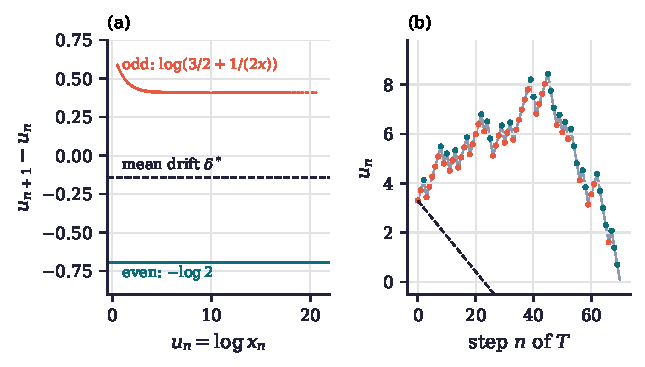
\includegraphics[width=\textwidth]{figures/ch5b_switched.pdf}
\caption{The Collatz recursion as a switched system in $u=\log x$. (a) Increments $u_{n+1}-u_n$ against $u_n$ along $60$ orbits started between $10^6$ and $10^7$; odd steps follow the curve $\log(3/2+1/(2x))$, even steps the constant $-\log2$, and the dashed line is the mean drift $\ds=\log(\sqrt3/2)$ of the Bernoulli model. (b) The orbit of $27$ under $T$, shaded by mode, with the drift line $\log27+n\ds$; every odd step rises and every even step falls.}
\label{fig:ch5b:switched}
\end{figure}

\section{Difference inequalities for the inverse tree}\label{sec:ch5b:tree}

The deepest unconditional lower bounds on how many integers reach $1$ come
from a different difference equation, one satisfied by counting functions on
the inverse tree\index{inverse tree}. Krasikov\index{Krasikov, I.}~\cite{krasikov1989} introduced the method, obtaining
the exponent $3/7$ from a system of inequalities modulo $9$; Applegate\index{Applegate, D.} and
Lagarias\index{Lagarias, J. C.}~\cite{applegate1995} reached $0.81$ by solving larger systems with
linear programming, and Krasikov and Lagarias~\cite{krasikov2003} enlarged the
systems further and reached the exponent $0.84$: for large $x$, at least
$x^{0.84}$ integers up to $x$ have orbits that reach $1$. We develop a simple
version of the method here, complete with proofs, which already gives an
exponent above $3/7$ and shows clearly where the difference inequalities\index{difference inequality} come
from. Accounts of the full method are in~\cite{krasikov2003,lagarias2010}.

\paragraph{The inverse tree.} Under $T$ every $n$ has the preimage $2n$, and
also the preimage $(2n-1)/3$ when $n\equiv2\pmod3$. Starting from a root $n$,
the \emph{doubling chain} $n,2n,4n,\dots$ lies in its inverse tree, and an
element $p=2^jn$ of the chain with $j\ge1$ has the odd preimage
\[
  c_j(n)=\frac{2^{j+1}n-1}{3}\qquad\text{when }2^jn\equiv2\pmod 3.
\]
If moreover $2^jn\equiv2$ or $8\pmod9$, then $c_j(n)\not\equiv0\pmod3$ and
$c_j(n)$ has odd preimages of its own; we call such $j$ \emph{fertile}. For
$n\not\equiv0\pmod3$ let
\[
  \pi_n(X)=\#\{m\le Xn:\ \text{the orbit of }m\text{ under }T\text{ passes through }n\}.
\]

\begin{lemma}[Difference inequality]\label{lem:ch5b:diffineq}
Let $n\not\equiv0\pmod3$ be an integer that does not lie on a cycle of $T$.
Then for every $X\ge1$,
\begin{equation}\label{eq:ch5b:diffineq}
  \pi_n(X)\;\ge\;\sum_{j\ \mathrm{fertile},\ 2^{j+1}\le3X}
  \pi_{c_j(n)}\Bigl(\frac{3X}{2^{j+1}}\Bigr).
\end{equation}
\end{lemma}

\begin{proof}
If $m$ is counted in $\pi_{c_j}(3X/2^{j+1})$ then its orbit passes through $c_j$,
hence through $T(c_j)=2^jn$ and then through $n$, and
$m\le(3X/2^{j+1})c_j=Xn-X/2^{j+1}<Xn$. So each term counts integers that are
also counted by $\pi_n(X)$. The sets for different fertile $j$ are disjoint:
the orbit of $m$ reaches $n$ for the first time along a unique path, which
passes through exactly one element of the doubling chain immediately after an
odd step, namely $2^jn=T(c_j)$; since $n$ is not on a cycle, the orbit cannot
reach $n$, leave it, and return through another branch.
\end{proof}

The inequality \eqref{eq:ch5b:diffineq} is a difference inequality, linear in the counting functions,
in the scale variable $\log X$: it bounds a counting function at scale $X$ by
the same family of functions at the smaller scales $3X/2^{j+1}$, with an index
$c_j(n)$ that moves through residue classes. The residue class of $c_j(n)$
modulo $3^k$ is determined by $n\bmod3^{k+1}$ and $j\bmod2\cdot3^k$, the period
of $2$ modulo $3^{k+1}$. This suggests a power law ansatz with a constant
depending on the class.

\begin{theorem}[Certified growth exponents]\label{thm:ch5b:exponent}
Fix $k\ge1$ and let $\mathcal R_k$ be the residues modulo $3^k$ prime to $3$.
For $g>0$ and a positive vector $(w_r)_{r\in\mathcal R_k}$ define
\[
  (\Phi_g w)_r=\min_{\ell}\ \sum_{j\ \mathrm{fertile\ for}\ \ell}
  \Bigl(\frac3{2^{j+1}}\Bigr)^g w_{[c_j(\ell)]},
\]
where the minimum is over the three lifts $\ell$ of $r$ to residues modulo
$3^{k+1}$, fertility and the class $[c_j(\ell)]\in\mathcal R_k$ depend only on
$\ell$ and $j$, and the sum is over all $j\ge1$. If $\Phi_g w\ge(1+\eta)w$
componentwise for some $\eta>0$, then there is $C>0$ such that
\[
  \pi_n(X)\;\ge\;C\,w_{[n]}\,X^g\qquad\text{for all }X\ge1
\]
and all $n\not\equiv0\pmod3$ not lying on a cycle of $T$.
\end{theorem}

\begin{proof}
The sum defining $\Phi_g$ converges, since its terms decay like $2^{-jg}$; by
the periodicity of the classes in $j$ it equals the sum over one period times
$1/(1-2^{-Pg})$ with $P=2\cdot3^k$. The terms with $2^{j+1}>3X$, which are
missing from \eqref{eq:ch5b:diffineq}, have total weight at most
$w_{\max}\sum_{2^{j+1}>3X}(3/2^{j+1})^g\le w_{\max}X^{-g}/(1-2^{-g})$,
which is below $\eta\,w_{\min}$ once $X\ge X_0$ for a suitable $X_0$. Choose
$C=1/(w_{\max}X_0^g)$, so that the claim holds for $X\le X_0$ because
$\pi_n(X)\ge1$ (the root itself is counted). For $X>X_0$ argue by strong induction
on the scale: every argument $3X/2^{j+1}$ in \eqref{eq:ch5b:diffineq} is at most
$3X/4<X$, and the children $c_j(n)$ are again prime to $3$ and not on a cycle
(an element of a cycle has its image on the cycle, and $T(c_j)=2^jn$ leads to
$n$). Hence
\begin{align*}
  \pi_n(X)&\ge C X^g\sum_{\substack{j\ \mathrm{fertile}\\2^{j+1}\le3X}}
  \Bigl(\frac3{2^{j+1}}\Bigr)^g w_{[c_j(n)]}\\
  &\ge CX^g\bigl((1+\eta)w_{[n]}-\eta w_{\min}\bigr)\ge CX^g w_{[n]},
\end{align*}
using that the full sum is at least $(\Phi_g w)_{[n]}$, because the lift of
$[n]$ determined by $n\bmod3^{k+1}$ is one of the three in the minimum.
\end{proof}

The theorem reduces a lower bound for an infinite family of counting
functions to a finite eigenvalue problem: find the largest $g$ for which the
monotone, homogeneous operator $\Phi_g$, nonlinear only through the minimum over lifts, has a positive supersolution. We solved
it by power iteration and bisection in $g$, and certified each exponent by
exhibiting a vector $w$ with $\min_r(\Phi_g w)_r/w_r>1$ (script
\texttt{ch5b\_tree.py}), and checked each certificate in exact integer arithmetic, with every power of $2$ and $3$ rounded down (script \texttt{ch5b\_tree\_exact.py}). The results are
\[
\begin{array}{c|cccccc}
k & 2 & 3 & 4 & 5 & 6 & 7\\\hline
\text{classes} & 6 & 18 & 54 & 162 & 486 & 1458\\
\gamma_k & 0.416 & 0.435 & 0.449 & 0.460 & 0.470 & 0.477
\end{array}
\]
with certified margins $1+\eta$ between $1.0002$ and $1.0027$.
The certificate for $k=7$ still has margin $1.0001$ at $g=0.47705$, so for the root $n=4$, which reaches $1$ and is not on a cycle, the theorem gives $\pi_4(X)\ge c\,X^{0.47705}$ for some $c>0$, which exceeds $(4X)^{0.477}$ for all large $X$. This gives the following.

\begin{corollary}[A counting bound]\label{cor:ch5b:count}
For all large $x$, at least $x^{0.477}$ integers $m\le x$ have orbits that
reach $1$.
\end{corollary}

The exponents increase with the modulus but slowly, and they are bounded by
what single doubling chains can produce. A mean field heuristic predicts the
limit. On average one third of the $j$ are fertile, and if the class constants
were all equal the supersolution condition would read
$\tfrac13\sum_{j\ge1}(3/2^{j+1})^g=1$, that is $3^{g-1}=2^g(2^g-1)$, whose root
is $g=0.4927$.
The exact counts of the doubling chain construction approach it: for roots $n=4,5,7$ the number of integers it generates below $Xn$ grows with exponent $0.500$, $0.502$ and $0.498$ over the last decade of $X$ up to $2^{20}$, and with exponent $0.492$, $0.494$ and $0.492$ over the last decade up to $2^{36}$ (script \texttt{ch5b\_chains.py}), while the true counting functions $\pi_n(X)$ grow with exponent $1.000$ (\cref{fig:ch5b:tree}).
The gap between $1/2$ and $0.84$ comes from a branch that the doubling chain system leaves out. Every element $p\equiv2\pmod3$ of the inverse tree has the odd preimage $(2p-1)/3<p$, the term $j=0$; seen from $p$, its count enters at the larger scale $3X/2$, so the induction on scale in the proof of \cref{thm:ch5b:exponent} cannot use it. With this branch the mean field equation becomes $\tfrac13\sum_{j\ge0}(3/2^{j+1})^g=1$, that is $3^{g-1}=2^g-1$, whose smaller root is exactly $g=1$. Krasikov's inequalities keep these terms, which Krasikov and Lagarias call advanced; Applegate and Lagarias truncated them to reach $0.81$, and Krasikov and Lagarias reached $0.84$ by proving that the linear programming bounds remain valid with the advanced terms present~\cite{krasikov2003}. The elements divisible by $3$ play no role: such an element has no odd preimage, so its inverse tree is a single doubling chain. The gap between $0.84$ and $1$ is open.
The exponent $1$ would already follow from a positive
proportion of integers reaching $1$, which is far short of the conjecture.

\begin{figure}[ht]
\centering
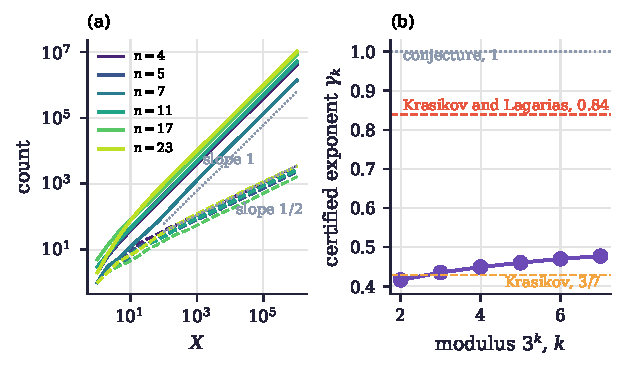
\includegraphics[width=\textwidth]{figures/ch5b_tree.pdf}
\caption{(a) Exact counting functions $\pi_n(X)$ (solid) and the counts produced
by the doubling chain construction (dashed) for several roots $n$, up to
$X=2^{20}$; the true counts grow linearly, the construction roughly like $X^{1/2}$. (b)
Certified exponents $\gamma_k$ from \cref{thm:ch5b:exponent} for moduli $3^k$,
against Krasikov's $3/7$, the exponent $0.84$ of Krasikov and Lagarias, and the
conjectured value $1$.}
\label{fig:ch5b:tree}
\end{figure}

\section{Momentum MM as a difference equation}\label{sec:ch5b:mm}

We now turn to the optimizers. For an $L$ smooth function $f$ the descent lemma
says that
\begin{equation}\label{eq:ch5b:major}
  f(y)\le Q_L(y\mid x):=f(x)+\langle\nabla f(x),y-x\rangle+\tfrac L2\|y-x\|^2
\end{equation}
for all $x,y$, with equality at $y=x$. So $Q_L(\cdot\mid x)$ majorizes $f$ in the
sense of \cref{chap:lyapunov}, and its minimizer is the gradient step
$G_{1/L}(x)=x-\nabla f(x)/L$. Gradient descent is the MM algorithm\index{MM algorithm} for this
majorizer\index{majorization}, and the MM descent property gives
$f(G_{1/L}(x))\le f(x)-\|\nabla f(x)\|^2/(2L)$.

Momentum methods of Nesterov's type majorize at a different point. Given an \emph{anchor}
$y_t=x_t+\beta_t(x_t-x_{t-1})$, they set $x_{t+1}=\arg\min_yQ_L(y\mid y_t)
=G_{1/L}(y_t)$. With $\beta_t\equiv\beta$ this is Nesterov's method; with
$\beta_t=\beta$ for odd $t$ and $\beta_t=0$ for even $t$ it is \smmdet. We call
the general scheme \emph{momentum\index{momentum} MM}: an MM iteration whose majorization point
is extrapolated on a schedule. Written out, it is the second order nonlinear
difference equation
\begin{equation}\label{eq:ch5b:momentummm}
  x_{t+1}=F_t(x_t,x_{t-1}):=y_t-\tfrac1L\nabla f(y_t),\qquad
  y_t=x_t+\beta_t(x_t-x_{t-1}),
\end{equation}
which is periodic in $t$ for Switching MM\index{Switching MM} and autonomous for Nesterov\index{Nesterov acceleration}.

Momentum MM gives up the monotonicity of MM: Nesterov's method, like heavy ball\index{heavy ball},
is not a descent method, and its function values oscillate. Switching MM
keeps it on alternate iterates, for every smooth function, convex or not.

\begin{proposition}[Monotonicity on alternate iterates]\label{prop:ch5b:monotone}
Let $f$ be $L$ smooth and bounded below by $f_{\inf}$, and run \smmdet\ with
step $1/L$ and $\beta\in[0,1)$. For even $t$,
\[
  f(x_{t+2})\le f(x_t)-\frac{1-\beta^2}{2L}\|\nabla f(x_t)\|^2
  -\frac1{2L}\|\nabla f(y_{t+1})\|^2 .
\]
Consequently $\min_{t<2K,\ t\ \mathrm{even}}\|\nabla f(x_t)\|^2\le
2L(f(x_0)-f_{\inf})/((1-\beta^2)K)$.
\end{proposition}

\begin{proof}
By \cref{lem:ch6:ystep}, $y_{t+1}=G_{(1+\beta)/L}(x_t)$ and
$x_{t+2}=G_{1/L}(y_{t+1})$. For a gradient step of length $h$ the descent lemma
gives $f(G_h(x))\le f(x)-h(1-Lh/2)\|\nabla f(x)\|^2$. With $h=(1+\beta)/L$ the
coefficient is $(1+\beta)(1-\beta)/(2L)$, and with $h=1/L$ it is $1/(2L)$. Adding
the two inequalities gives the first claim, and summing over $K$ periods gives
the second.
\end{proof}

The extrapolation is safe because it is a gradient step of length
$(1+\beta)/L<2/L$, inside the range where the descent lemma still guarantees
decrease. Momentum at every step has no such interpretation: its anchor
carries the whole history of past gradients.

\section{Stability theory}\label{sec:ch5b:stability}

\subsection{Lyapunov functions for difference equations}

A function $V\ge0$ is a Lyapunov function\index{Lyapunov function} for the difference equation
$z_{t+1}=F_t(z_t)$ with rate $\rho<1$ if $V(z_{t+1})\le\rho V(z_t)$ for all $t$
and $z_t$; then $V(z_t)\le\rho^tV(z_0)$. For gradient descent on a $\mu$ strongly
convex, $L$ smooth function, $V=f-f^*$ works with $\rho=1-1/\kappa$. For
Nesterov\index{Nesterov acceleration}'s method with constant momentum\index{momentum} $\beta=(\sqrt\kappa-1)/(\sqrt\kappa+1)$
and step $1/L$, Nesterov\index{Nesterov, Yu.}'s estimate sequence construction gives the Lyapunov
function $f(x_t)-f^*+\frac\mu2\|v_t-x^*\|^2$, with $v_t$ an auxiliary sequence that
is an affine combination of $x_t$ and $x_{t-1}$, and the rate
$1-1/\sqrt\kappa$: for every $t$,
\[
  f(x_t)-f^*\le\Bigl(1-\frac1{\sqrt\kappa}\Bigr)^t\Bigl(f(x_0)-f^*
  +\frac\mu2\|x_0-x^*\|^2\Bigr),
\]
see~\cite{nesterov2004}, and~\cite{wilson2021} for the Lyapunov reading.
The point to retain is that the Lyapunov function of an accelerated method must involve two consecutive iterates, because the state of the method is the pair $(x_t,x_{t-1})$: started at $x_t=x^*$ with $x_{t-1}\ne x^*$ the method in general leaves the minimizer, so no function of $x_t$ alone that vanishes only at $x^*$ can decrease at every step.

\subsection{Switching and the joint spectral radius}

On one eigendirection of a quadratic, with $a=\alpha\lambda$ and state
$z_t=(e_t,e_{t-1})$, the two steps of \smmdet\ are the matrices
\[
  D=\begin{pmatrix}1-a&0\\1&0\end{pmatrix},\qquad
  N=\begin{pmatrix}(1-a)(1+\beta)&-(1-a)\beta\\1&0\end{pmatrix},
\]
for a descent and an injection respectively. \smmdet\ applies them in the
periodic order $D,N,D,N,\dots$, every step Nesterov\index{Nesterov acceleration} applies $N$ always, and the
adaptive rule \smmstate\ of \cref{chap:smm} applies them in an order that depends on the state.
What can be said for an \emph{arbitrary} order? The relevant quantity is the
joint spectral radius\index{joint spectral radius} of Rota\index{Rota, G. C.} and Strang\index{Strang, G.}~\cite{rota1960},
\[
  \hat\rho(\{D,N\})=\lim_{k\to\infty}\max_{M_i\in\{D,N\}}
  \|M_k\cdots M_1\|^{1/k},
\]
which is the best possible exponential rate valid for every switching sequence;
see~\cite{jungers2009} for the theory. It is in general hard to compute. Here it
is not, because $D$ has rank one.

\begin{proposition}[Exact joint spectral radius]\label{prop:ch5b:jsr}
Write $D=vu^\top$ with $u=(1,0)^\top$ and $v=(1-a,1)^\top$, and put
$\tau_j=u^\top N^jv$, the first coordinate after $j$ injections started from
the state left by one descent step. Then
\[
  \hat\rho(\{D,N\})=\max\Bigl(\rho(N),\ \sup_{j\ge0}|\tau_j|^{1/(j+1)}\Bigr).
\]
\end{proposition}

\begin{proof}
By the theorem of Berger\index{Berger, M. A.} and Wang\index{Wang, Y.} (see~\cite{jungers2009}) the joint spectral
radius equals $\limsup_k\max\rho(M_k\cdots M_1)^{1/k}$ over products, and by
cyclic invariance of the spectrum it suffices to consider products that are
either $N^k$ or begin with $D$. A product beginning with $D$ is, up to cyclic
permutation, $DN^{j_1}DN^{j_2}\cdots DN^{j_m}$ with $\sum(j_i+1)=k$. Since
$D=vu^\top$, this product equals $v\,\bigl(\prod_{i}u^\top N^{j_i}v\bigr)$ times
$u^\top$ in the appropriate order, a rank one matrix with the single nonzero
eigenvalue $\prod_i\tau_{j_i}$. Hence $\rho^{1/k}=\prod_i|\tau_{j_i}|^{1/k}\le
\max_i|\tau_{j_i}|^{1/(j_i+1)}$, with equality when all $j_i$ are equal. Taking
the supremum over products gives the formula.
\end{proof}

The formula needs only the scalar sequence $\tau_j$, which tends to zero
geometrically at rate $\rho(N)<1$, so the maximum in the formula is attained, at a finite $j$ or by $\rho(N)$,
and can be computed to any accuracy (script \texttt{ch5b\_jsr.py}). The result
is striking (\cref{fig:ch5b:jsr}). For every $a$ we computed the joint spectral
radius is below $1$, and it exceeds the larger of the two pure rates, $\max(\rho(D),
\rho(N))$, by at most $0.0056$ at $\beta=\lt-1$ and $0.0011$ at $\beta=0.9$, over
a grid of $400$ values of $a$ from $10^{-4}$ to $0.999$. For small $a$ it equals
$1-a$, the rate of gradient descent, attained by the product $D$ alone.

Since $\tau_j\to0$, the joint spectral radius is below $1$ exactly when
$|\tau_j|<1$ for every $j$.
Over a grid of $200$ values of $\beta\in[0,0.999]$ and $300$ values of $a\in[10^{-5},0.9999]$ we found $\sup_j|\tau_j|=\tau_0=1-a$ in every case, with a quadratic Lyapunov function of $N$ bounding the terms beyond those computed (script \texttt{ch5b\_transient.py}): the transient of the injection steps never exceeds the first descent.
We record this as a conjecture.

\begin{conjecture}[Transient bound]\label{conj:ch5b:transient}
For all $a\in(0,1]$, $\beta\in[0,1)$ and $j\ge0$, $|\tau_j|\le1-a$.
\end{conjecture}

Note that while $e$ stays positive the bound is immediate: with
$d_t=e_{t-1}-e_t$ one has $e_{t+1}=(1-a)(e_t-\beta d_t)$ and
$d_{t+1}=ae_t+(1-a)\beta d_t$, with $e_0=1-a$ and $d_0=a$. As long as $e$ stays
nonnegative, $d$ stays nonnegative and $e_{t+1}\le(1-a)e_t$, so $e$ decreases
and $|e_t|\le1-a$. The difficulty is the oscillating regime after $e$ changes
sign.

\begin{corollary}[Every switching rule is stable]\label{cor:ch5b:anyswitch}
Fix $a\in(0,1)$ and suppose $|\tau_j|<1$ for all $j$, as
\cref{conj:ch5b:transient} asserts and as computation confirms on the grid
above. Then on a quadratic with spectrum in $(0,L]$ and step $1/L$, every
switching sequence between descent and injection steps, whether periodic,
random, or chosen adaptively from the state as in \smmstate, converges to the
minimizer on the eigendirection with $a=\alpha\lambda$, with exponential rate at
most $\hat\rho(\{D(a),N(a)\})<1$.
\end{corollary}

This is partial progress on open problem S4 of \cref{chap:open}. At every grid point above, and for all $a$ and $\beta$ if \cref{conj:ch5b:transient} holds, adaptive switching cannot destabilize the method. On the grid of $400$ values of $a$ it also cannot make the contraction factor more than $0.0056$ larger than that of the worse of gradient descent and every step Nesterov at $\beta=\lt-1$, which is about one percent per step and $1.8$ percent in the number of iterations, and at $\beta=0.9$ the cost is $0.12$ percent per step and $1.1$ percent in iterations. Stability alone does not close the noiseless gap to every step momentum that S4 asks about.
The Collatz switched system\index{switched system} \eqref{eq:ch5b:switched} is the opposite case: there
the joint behaviour under arbitrary switching is unstable, and all the
difficulty lies in the switching signal.

\begin{figure}[ht]
\centering
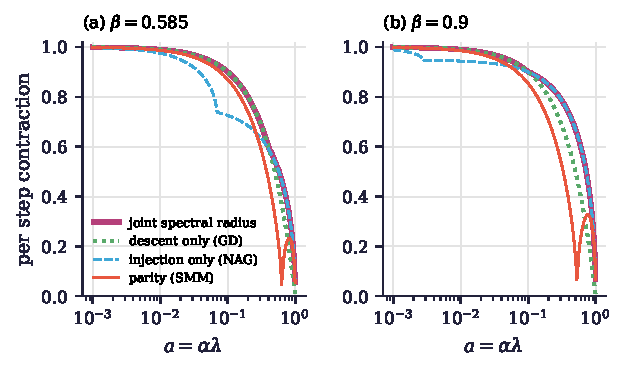
\includegraphics[width=\textwidth]{figures/ch5b_jsr.pdf}
\caption{The joint spectral radius of the descent and injection matrices,
computed exactly by \cref{prop:ch5b:jsr}, against $a=\alpha\lambda$, together
with the per step rates of pure descent (gradient descent), pure injection
(every step Nesterov) and the parity schedule of \smmdet. The joint spectral
radius hugs the upper envelope of the two pure rates.}
\label{fig:ch5b:jsr}
\end{figure}

\section{A linear rate beyond quadratics}\label{sec:ch5b:rate}

\Cref{thm:smmquad} described \smmdet\ exactly on quadratics. For a general
smooth strongly convex function the same identity, \cref{lem:ch6:ystep}, holds
with no change, and it reduces the convergence question to the classical
contraction of a single gradient step.

\begin{theorem}[Linear rate of \smmdet]\label{thm:ch5b:rate}
Let $f$ be $\mu$ strongly convex and $L$ smooth with minimizer $x^*$, put
$\kappa=L/\mu$, and run \smmdet\ with step $\alpha=1/L$ and $\beta\in[0,1)$. For
every even $t$,
\begin{gather*}
  \|x_{t+2}-x^*\|\le q\,\|x_t-x^*\|,\\
  q=q(\beta,\kappa)=\Bigl(1-\frac1\kappa\Bigr)\max\Bigl(1-\frac{1+\beta}\kappa,\
  \beta\Bigr),
\end{gather*}
and $f(x_{t+2})-f^*\le q^2\,(f(x_t)-f^*)$.
\end{theorem}

\begin{proof}
By \cref{lem:ch6:ystep}, $x_{t+2}=G_{1/L}(G_{(1+\beta)/L}(x_t))$. For a step
$h\in(0,2/L)$ and $f$ twice differentiable,
$G_h(x)-x^*=x-x^*-h(\nabla f(x)-\nabla f(x^*))=(I-h\bar H)(x-x^*)$ with
$\bar H=\int_0^1\nabla^2f(x^*+s(x-x^*))\,ds$, whose eigenvalues lie in
$[\mu,L]$. Hence $\|G_h(x)-x^*\|\le\max(|1-h\mu|,|1-hL|)\|x-x^*\|$; for $f$ that
is only once differentiable the same bound follows by smoothing, or directly
from the cocoercivity of $\nabla f$. With $h=(1+\beta)/L$ the factor is
$\max(1-(1+\beta)/\kappa,\beta)$, and with $h=1/L$ it is $1-1/\kappa$. Composing
gives the distance bound.
For function values, Taylor\index{Taylor, A. B.}, Hendrickx\index{Hendrickx, J. M.} and Glineur\index{Glineur, F.}~\cite[Theorem~3.3]{taylor2018} show that a gradient step of length $h\in(0,2/L)$ satisfies $f(G_h(x))-f^*\le\max((1-h\mu)^2,(1-hL)^2)(f(x)-f^*)$; composing the two steps gives the second bound.
\end{proof}

How good is this? The contraction of each gradient step is tight for the class,
so one might worry only about the composition. We computed the exact worst case
of two steps of \smmdet\ over all $\mu$ strongly convex, $L$ smooth functions in
every dimension by \emph{performance estimation\index{performance estimation}}~\cite{drori2014,taylor2017}: the
worst case is the value of a small semidefinite program built from the
interpolation conditions of the class (script \texttt{ch5b\_pep.py}). For
$\beta\in\{0.3,\lt-1,0.9\}$ and $\kappa\in\{2,3,5,10,20,50,100\}$ the worst case
of $\|x_{t+2}-x^*\|^2/\|x_t-x^*\|^2$ agreed with $q^2$ to six digits in all $21$
cases.
So the distance bound of \cref{thm:ch5b:rate} is the exact worst case, not merely a bound, and explicit functions attain it for every $\kappa$. When $\kappa\ge(1+\beta)/(1-\beta)$, which is $\kappa\ge3.82$ at $\beta=\lt-1$, both factors are attained at the eigenvalue $\mu$ and the worst case is the quadratic $\frac\mu2\|x\|^2$. For smaller $\kappa$ the two factors are attained at different curvatures, and the worst function is not quadratic: the one dimensional function equal to $\frac L2x^2$ for $x\ge0$ and to $\frac\mu2x^2$ for $x<0$ attains $q$, since from $x_t=1$ the long step lands at $-\beta$ and the short step at $-\beta(1-1/\kappa)$.
The function value bound $q^2$ is exact only for $\kappa\ge(1+\beta)/(1-\beta)$, where the same quadratic attains it. Below that threshold performance estimation for function values gives a smaller worst case, for example $0.049$ against $q^2=0.086$ at $\beta=\lt-1$ and $\kappa=2$.

\begin{corollary}[Speed relative to gradient descent]\label{cor:ch5b:speed}
For $\kappa\ge(1+\beta)/(1-\beta)$ the per step rate of \smmdet\ is
$q^{1/2}=((1-1/\kappa)(1-(1+\beta)/\kappa))^{1/2}$, so that
$-\kappa\log q^{1/2}\to(2+\beta)/2$ as $\kappa\to\infty$, against $1$ for gradient
descent with the same step. This is the effective step multiplier of
\cref{cor:ch6:slow}, now valid on the whole class.
\end{corollary}

\Cref{fig:ch5b:rate} plots the normalized rate $-\kappa\log q/2$ against $\kappa$.
It lies below gradient descent exactly when $\kappa<1/(1-\beta)$, which is $\kappa<2.41$ at $\beta=\lt-1$: there the long step $(1+\beta)/L$ overshoots the large curvatures and the factor $\beta$ dominates. On the range of the figure it is largest at $\kappa=(1+\beta)/(1-\beta)$, where the two factors of $q$ balance ($1.60$ at $\beta=\lt-1$), and beyond that point it decreases to $(2+\beta)/2$, which is $1.29$ at $\beta=\lt-1$, as $\kappa\to\infty$.
Open problem S1 asked for exactly this:
a linear rate on the whole class with the constant predicted by the quadratic
analysis. The answer is that the quadratic constant is exact for $\kappa\ge(1+\beta)/(1-\beta)$, and in particular as $\kappa\to\infty$.

\begin{figure}[ht]
\centering
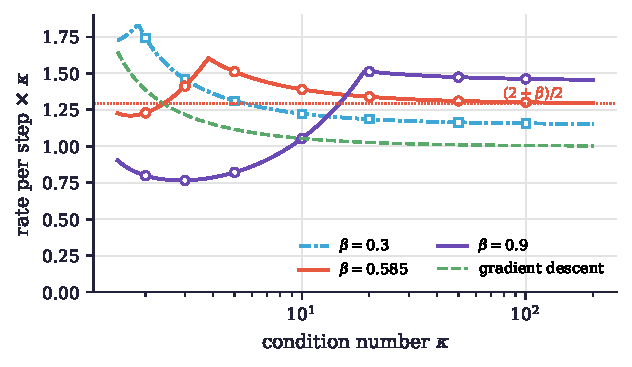
\includegraphics[width=\textwidth]{figures/ch5b_rate.pdf}
\caption{Worst case per step rate of \smmdet\ for the distance to the minimizer on the class of $\mu$ strongly
convex, $L$ smooth functions, multiplied by $\kappa$, from
\cref{thm:ch5b:rate} (lines) and from performance estimation (open markers), for
three values of $\beta$; gradient descent with step $1/L$ is dashed. At large
$\kappa$ the normalized rate of \smmdet\ tends to $(2+\beta)/2$.}
\label{fig:ch5b:rate}
\end{figure}

\section{Continuous time limits}\label{sec:ch5b:ode}

The continuous time view of \cref{chap:momentum} describes accelerated methods by
second order differential equations, obtained by letting the step size tend to
zero while the momentum\index{momentum} tends to one at a matched rate: for heavy ball\index{heavy ball} with
step $s$ and $\beta=1-c\sqrt s$, the limit is the damped oscillator
$\ddot x+c\dot x+\nabla f(x)=0$ on the time scale $t=k\sqrt s$, and Nesterov\index{Nesterov acceleration}'s
method with $\beta_k=(k-1)/(k+2)$ gives the equation of Su\index{Su, W.}, Boyd\index{Boyd, S.} and
Cand\`es\index{Candes, E. J.@Cand\`es, E. J.}~\cite{su2016}. With $\beta$ \emph{fixed} and $\alpha\to0$ the picture is
different, and it is the relevant one for a fixed default such as
$\beta=\lt-1$.

\begin{proposition}[Modified equation for period two steps]\label{prop:ch5b:modified}
Let $f$ be three times differentiable and consider the composition of gradient
steps of lengths $h_1$ and $h_2$, in either order. To second order in
$h=h_1+h_2$ it agrees with the time $h$ flow of the modified equation\index{modified equation}
\begin{equation}\label{eq:ch5b:modified}
\begin{aligned}
  \dot x&=-\nabla f(x)-\frac{h_1^2+h_2^2}{2(h_1+h_2)}\,\nabla^2f(x)\nabla f(x)\\
  &=-\nabla\Bigl(f+\frac{\bar h}{4}\|\nabla f\|^2\Bigr),\qquad
  \bar h=\frac{h_1^2+h_2^2}{h_1+h_2}.
\end{aligned}
\end{equation}
\end{proposition}

\begin{proof}
Write $g=\nabla f$ and $H=\nabla^2f$. Expanding,
$G_{h_2}(G_{h_1}(x))=x-h_1g-h_2g(x-h_1g)+O(h^3)=x-hg+h_1h_2Hg+O(h^3)$, and the
term $h_1h_2Hg$ is symmetric in the two steps. The time $h$ flow of
$\dot x=-g-cHg$ is $x-hg-hcHg+\frac{h^2}2Hg+O(h^3)$, because the second
derivative of the flow is $Hg$ to leading order. Matching the coefficients of
$Hg$ gives $-hc+h^2/2=h_1h_2$, so $c=(h^2/2-h_1h_2)/h=(h_1^2+h_2^2)/(2h)$. Finally
$Hg=\nabla(\frac12\|g\|^2)$.
\end{proof}

For a single gradient step of length $h$ the same computation gives the
modified function $f+\frac h4\|\nabla f\|^2$, the implicit gradient
regularization of Barrett\index{Barrett, D. G. T.} and Dherin\index{Dherin, B.}~\cite{barrett2021}; backward error analysis
of this kind is classical in geometric numerical
integration~\cite{hairer2006}. For \smmdet, $h_1=(1+\beta)\alpha$ and
$h_2=\alpha$, so the iteration follows the gradient flow of
\[
  f+\frac{\alpha V(\beta)}{4}\|\nabla f\|^2,\qquad
  V(\beta)=\frac{(1+\beta)^2+1}{2+\beta},
\]
on the time scale $(2+\beta)\alpha/2$ per iteration; $V(\beta)$ is the slow mode noise amplification of \cref{cor:ch7:slow}. Two conclusions follow.

First, Switching MM\index{Switching MM} has no inertial limit. Whatever the value of $\beta<1$, its
continuous time limit is a first order gradient flow, sped up by the factor
$(2+\beta)/2$ and implicitly regularized. This is the continuous counterpart of
\cref{rem:ch6:reframing}: the method carries one gradient of memory, not a
velocity, and no rescaling turns it into a damped oscillator.

Second, the implicit regularization\index{implicit regularization} strength has a familiar ratio. Gradient
descent run at the same speed, with step $(2+\beta)\alpha/2$, has regularization
coefficient $(2+\beta)\alpha/8$, while \smmdet\ has $V(\beta)\alpha/4$. Their
ratio is
\[
  \frac{2V(\beta)}{2+\beta}=\frac{2\bigl((1+\beta)^2+1\bigr)}{(2+\beta)^2}
  =1+\frac{\beta^2}{(2+\beta)^2},
\]
exactly the noise floor\index{noise floor} penalty of \cref{prop:ch7:matched} and of the gain weight\index{gain weight theorem}
theorem, \cref{thm:ch7:gainweight}. This is not a coincidence. Both quantities are the ratio of the mean
square step to the square of the mean step, $\frac12(h_1^2+h_2^2)/
(\frac12(h_1+h_2))^2$, which Cauchy and Schwarz bounds below by $1$. Unequal steps
cost the same factor whether one measures the stationary noise or the implicit
bias.

\section*{Notes}

The stability of switched systems\index{switched system} under arbitrary and constrained switching
is surveyed by Liberzon\index{Liberzon, D.}~\cite{liberzon2003}; the joint spectral radius\index{joint spectral radius} is due to
Rota and Strang~\cite{rota1960}, and Jungers\index{Jungers, R.}~\cite{jungers2009} covers both
its computation and the theorem of Berger and Wang. The difference inequality\index{difference inequality} method
for the inverse Collatz tree is due to Krasikov\index{Krasikov, I.}~\cite{krasikov1989}, with
improvements by Applegate and Lagarias\index{Lagarias, J. C.}~\cite{applegate1995} and the sharpest
results by Krasikov and Lagarias~\cite{krasikov2003}; the survey volume~\cite{lagarias2010}
gives the history. The doubling chain system, \cref{thm:ch5b:exponent} and its
certified exponents are our simplified version and are far from the state of
the art. The view of gradient descent as an MM algorithm\index{MM algorithm} through the descent
lemma is standard~\cite{lange2000,hunter2004}; the name momentum\index{momentum} MM, the
monotonicity and joint spectral radius propositions, and the rate theorem are
ours, with the
function value step bound taken from Taylor, Hendrickx and
Glineur~\cite{taylor2018}.
For finite sets of rank one matrices, Ahmadi\index{Ahmadi, A. A.} and Parrilo\index{Parrilo, P. A.}~\cite{ahmadi2012} reduce the joint spectral radius in the same way to products around cycles, a maximum cycle mean problem; \cref{prop:ch5b:jsr}, with one matrix of rank one, is a variant of their device.
Performance estimation was introduced by Drori\index{Drori, Y.} and
Teboulle\index{Teboulle, M.}~\cite{drori2014} and made exact for smooth strongly convex functions by
Taylor, Hendrickx and Glineur~\cite{taylor2017}. Modified equations and backward
error analysis are treated in~\cite{hairer2006}, and their use for implicit
regularization in~\cite{barrett2021}.

\section*{Exercises}

\begin{exercise}
Show that under arbitrary switching the system \eqref{eq:ch5b:switched} can realize every sequence of modes, that while $u_n\ge0$ every increment lies in $\{-\log2\}\cup(\log\frac32,\log2]$, and that a run of mode $1$ increments is strictly decreasing. Show also that for the actual Collatz signal no two consecutive steps of the standard map\index{standard map} $T_0$ are odd.
What does this say about the
frequencies achievable under $T_0$?
\end{exercise}

\begin{exercise}
Compute by hand the operator $\Phi_g$ of \cref{thm:ch5b:exponent} for $k=1$,
with classes $1,2\bmod3$ and lifts modulo $9$, and find the largest $g$ for
which it has a positive supersolution. Compare with the values in the table.
\end{exercise}

\begin{exercise}
Verify the mean field equation $3^{g-1}=2^g(2^g-1)$ and show that it has a
unique root in $(0,1)$. Explain why the doubling chain construction cannot give
an exponent above this root for typical roots.
\end{exercise}

\begin{exercise}
Show that \cref{prop:ch5b:monotone} fails for every step heavy ball\index{heavy ball}: construct
an $L$ smooth convex quadratic in one dimension and a starting point for which
$f(x_{t+2})>f(x_t)$ for some even $t$ with $\beta=0.585$ and step $1/L$.
\end{exercise}

\begin{exercise}
Compute $\tau_0,\tau_1,\tau_2$ of \cref{prop:ch5b:jsr} in closed form and
show that $|\tau_1|^{1/2}$ is the per step rate of the periodic schedule. For
which $a$ does the supremum in the proposition occur at $j=0$?
\end{exercise}

\begin{exercise}
Using \cref{thm:ch5b:rate}, find the value of $\beta$ that minimizes $q(\beta,\kappa)$
for a given $\kappa$, and show that it tends to $1$ as $\kappa\to\infty$. Compare
the resulting rate with gradient descent and with Nesterov\index{Nesterov acceleration}'s optimal
$1-1/\sqrt\kappa$.
\end{exercise}

\chapter{Three Point Inequalities and Similar Triangles}\label{chap:threepoint}

Every convergence proof for an MM algorithm or an accelerated gradient method
rests, at bottom, on one inequality. It compares the new iterate with an
arbitrary reference point through three distances, and in its Euclidean form
it is nothing more than the law of cosines for the triangle formed by the old
iterate, the new iterate and the reference point. Nesterov's accelerated
method can be organized around it as a sequence of similar triangles, and the
energy that decreases along the iterates is assembled from it. This chapter
works the inequality as hard as it will go. We prove it, use it to derive the
classical rates, and then turn it on the two objects of this book.

On Switching MM it gives something new. A three point argument proves that
on smooth convex functions, which need not be strongly convex, two steps of
Switching MM are worth $2+\beta$ steps of gradient descent rather than two,
provided the long step $1+\beta$ is at most the golden ratio. Performance
estimation then indicates that the resulting rate, after the usual tightening,
is exact: we conjecture that the worst case of Switching MM is $LR^2/((4+2\beta)N+2)$, a factor
$1+\beta/2$ below gradient descent, for every $\beta$ up to a threshold
$\beta_2=0.686$ that we compute in closed form. Every step momentum at the Collatz value of
$\beta$ is worse than gradient descent in the worst case for $4\le N\le15$ and only slightly better for $16\le N\le20$, so on this
measure the parity schedule wins. Acceleration in the sense of a $1/N^2$
rate requires the similar triangles, and we show that it survives arbitrary
switching with plain gradient steps.

On the Collatz map the answer is half yes. The three point identity holds
exactly, with the book's own majorizer of the logarithm: each step of the
Syracuse map splits into a linear term, which is a martingale in the model,
and a Bregman divergence, which dissipates at least a fixed amount at every
step. What is missing is the other half of the three point inequality, the
optimality of the step, and we explain exactly why it cannot be supplied.

\section{The three point identity and the three point inequality}\label{sec:ch7b:threepoint}

Let $h$ be a differentiable convex function on a convex set, and write
\[
  D_h(a,b)=h(a)-h(b)-\langle\nabla h(b),a-b\rangle\ \ge0
\]
for its Bregman divergence. For $h=\half\|\cdot\|^2$ this is
$\half\|a-b\|^2$; for the negative entropy $h(x)=\sum_ix_i\log x_i$ on the
simplex it is the Kullback and Leibler divergence; for $h=-\log$ on the
positive reals it is the Itakura and Saito divergence
$D(a,b)=a/b-1-\log(a/b)$, which will reappear in \cref{sec:ch7b:collatz}.

\begin{lemma}[Three point identity]\label{lem:ch7b:identity}
For all $u,z,z^+$ in the domain of $h$,
\[
  D_h(u,z)-D_h(u,z^+)-D_h(z^+,z)=\langle\nabla h(z^+)-\nabla h(z),\,u-z^+\rangle.
\]
For $h=\half\|\cdot\|^2$ it reads
$2\langle z-z^+,\,u-z^+\rangle=\|u-z^+\|^2+\|z-z^+\|^2-\|u-z\|^2$, which is
the law of cosines for the triangle with vertices $u$, $z$ and $z^+$.
\end{lemma}

\begin{proof}
Expand the three divergences from the definition. The values $h(u)$, $h(z)$
and $h(z^+)$ cancel in pairs, and the inner products collect to the right
hand side.
\end{proof}

\begin{lemma}[Three point inequality]\label{lem:ch7b:inequality}
Let $\psi$ be convex, let $C$ be a closed convex set, and let
\[
  z^+=\arg\min_{x\in C}\bigl\{\psi(x)+D_h(x,z)\bigr\}.
\]
Then for every $u\in C$,
\[
  \psi(z^+)+D_h(z^+,z)\;\le\;\psi(u)+D_h(u,z)-D_h(u,z^+).
\]
\end{lemma}

\begin{proof}
Since $z^+$ minimizes a convex function over a convex set, there is a
subgradient $\xi\in\partial\psi(z^+)$ with the variational inequality
$\langle\xi+\nabla h(z^+)-\nabla h(z),\,u-z^+\rangle\ge0$ for every $u\in C$.
By convexity $\psi(u)\ge\psi(z^+)+\langle\xi,u-z^+\rangle$. Adding the two
and using \cref{lem:ch7b:identity} for the term in $\nabla h$ gives the claim.
\end{proof}

The proof has two ingredients and it is worth keeping them apart. The first
is the identity, which is pure geometry and holds for any three points. The
second is the variational inequality, which holds because $z^+$ is the
minimizer of a convex function over a convex set. The identity is
bookkeeping; the variational inequality is where the information enters.
\Cref{fig:ch7b:geometry}(a) shows the Euclidean case: the step from $z$ to
$z^+$ is a move against a gradient, and the inequality says that the angle at
$z^+$ in the triangle $(u,z,z^+)$ is not acute in the direction that would let
$z^+$ drift away from $u$.

\begin{figure}[t]
\centering
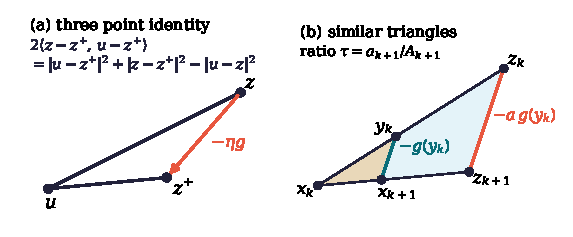
\includegraphics[width=\textwidth]{figures/ch5d_geometry.pdf}
\caption{(a) The three point identity is the law of cosines for the triangle
formed by a reference point $u$, an iterate $z$ and the next iterate $z^+$. (b)
The method of similar triangles: the gradient point $y_k$ and the new iterate
$x_{k+1}$ are the images of $z_k$ and $z_{k+1}$ under the homothety with centre
$x_k$ and ratio $\tau=a_{k+1}/A_{k+1}$, so the two shaded triangles are
similar.}
\label{fig:ch7b:geometry}
\end{figure}

\section{MM convergence from the inequality}\label{sec:ch7b:mm}

Let $f$ be convex and $L$ smooth relative to $h$, in the sense of Bauschke,
Bolte and Teboulle~\cite{bauschke2017} and Lu, Freund and
Nesterov~\cite{lu2018}:
\[
  f(x)\le f(z)+\langle\nabla f(z),x-z\rangle+L\,D_h(x,z)\qquad\text{for all }x,z.
\]
The right hand side, as a function of $x$, is a majorizer\index{majorization} of $f$ that touches
it at $z$, and minimizing it is an MM step\index{MM algorithm}. For $h=\half\|\cdot\|^2$ the
condition is ordinary $L$ smoothness and the MM step is the gradient step
$z^+=z-\nabla f(z)/L$; for the entropy on the simplex it is the exponentiated
gradient update.

\begin{theorem}[MM rate from the three point inequality]\label{thm:ch7b:mm}
Let
\[
  z_{k+1}=\arg\min_{x\in C}\{f(z_k)+\langle\nabla f(z_k),x-z_k\rangle+LD_h(x,z_k)\}.
\]
Then for every $u\in C$ and every $k\ge1$,
\[
  f(z_k)-f(u)\;\le\;\frac{L\,D_h(u,z_0)}{k}.
\]
\end{theorem}

\begin{proof}
Apply \cref{lem:ch7b:inequality} with $\psi(x)=\langle\nabla f(z_k),x\rangle/L$:
\begin{multline*}
  \langle\nabla f(z_k),z_{k+1}\rangle+L\,D_h(z_{k+1},z_k)\\
  \le\langle\nabla f(z_k),u\rangle+L\,D_h(u,z_k)-L\,D_h(u,z_{k+1}).
\end{multline*}
Relative smoothness bounds $f(z_{k+1})$ by $f(z_k)$ plus the left hand side
minus $\langle\nabla f(z_k),z_k\rangle$, and convexity bounds
$f(z_k)+\langle\nabla f(z_k),u-z_k\rangle$ by $f(u)$. Together,
$f(z_{k+1})-f(u)\le L\,D_h(u,z_k)-L\,D_h(u,z_{k+1})$. Summing over the first
$k$ steps telescopes the right hand side, and since the MM step never
increases $f$, the left hand side is at least $k(f(z_k)-f(u))$.
\end{proof}

For gradient descent this is the familiar bound $LR^2/(2k)$ with
$R=\|z_0-x_*\|$. It is not tight: the exact worst case, found by Drori and
Teboulle~\cite{drori2014} by performance estimation\index{performance estimation}, is $LR^2/(4k+2)$. The factor
two is what a cleverer combination of the same inequalities gains, and we will
meet it again.

\section{Similar triangles and acceleration}\label{sec:ch7b:triangles}

Acceleration keeps the three point inequality and changes what it is
applied to. Nesterov's method in the form of the \emph{method of similar
triangles} of Gasnikov and Nesterov~\cite{gasnikov2018} runs three sequences.
Start from $x_0=z_0$ and $A_0=0$. At step $k$ choose $a_{k+1}>0$ with
$L\,a_{k+1}^2=A_{k+1}$, where $A_{k+1}=A_k+a_{k+1}$, and set
\begin{gather*}
  y_k=\frac{A_kx_k+a_{k+1}z_k}{A_{k+1}},\qquad
  z_{k+1}=z_k-a_{k+1}\nabla f(y_k),\\
  x_{k+1}=\frac{A_kx_k+a_{k+1}z_{k+1}}{A_{k+1}}=y_k-\frac1L\nabla f(y_k).
\end{gather*}
The point $y_k$ divides the segment from $x_k$ to $z_k$ in the ratio
$\tau=a_{k+1}/A_{k+1}$, and $x_{k+1}$ divides the segment from $x_k$ to $z_{k+1}$
in the same ratio, so the triangle $(x_k,y_k,x_{k+1})$ is the image of
$(x_k,z_k,z_{k+1})$ under a homothety with centre $x_k$
(\cref{fig:ch7b:geometry}(b)). The $z$ sequence takes long steps with growing
weights $a_{k+1}$; the $x$ sequence takes ordinary gradient steps from the
points $y_k$; the similar triangles tie them together. The form
$x_{k+1}=y_k-\nabla f(y_k)/L$ follows from
$x_{k+1}-y_k=\tau(z_{k+1}-z_k)=-\tau a_{k+1}\nabla f(y_k)$ and
$\tau a_{k+1}=a_{k+1}^2/A_{k+1}=1/L$.

\begin{theorem}[The energy of similar triangles]\label{thm:ch7b:triangles}
Let $f$ be convex and $L$ smooth with a minimizer $x_*$, and put
\[
  E_k=A_k\bigl(f(x_k)-f_*\bigr)+\half\|z_k-x_*\|^2.
\]
Then $E_{k+1}\le E_k$ for every $k$, and $A_k\ge k^2/(4L)$, so that
\[
  f(x_k)-f_*\;\le\;\frac{2L\|x_0-x_*\|^2}{k^2}.
\]
\end{theorem}

\begin{proof}
Write $g=\nabla f(y_k)$, $A=A_k$, $A'=A_{k+1}$, $a=a_{k+1}$. The $z$ step is the
minimizer of $a\langle g,x\rangle+\half\|x-z_k\|^2$, so \cref{lem:ch7b:inequality}
with $u=x_*$ gives
\begin{equation}\label{eq:ch7b:zstep}
  a\langle g,z_{k+1}-x_*\rangle\le\half\|x_*-z_k\|^2-\half\|x_*-z_{k+1}\|^2-\half\|z_{k+1}-z_k\|^2.
\end{equation}
The descent lemma at $y_k$, with $x_{k+1}-y_k=(a/A')(z_{k+1}-z_k)$ and
$La^2=A'$, gives
\[
  A'f(x_{k+1})\le A'f(y_k)+a\langle g,z_{k+1}-z_k\rangle+\half\|z_{k+1}-z_k\|^2.
\]
Split $a\langle g,z_{k+1}-z_k\rangle=a\langle g,z_{k+1}-x_*\rangle+a\langle g,x_*-z_k\rangle$
and use \eqref{eq:ch7b:zstep} on the first part; the terms in
$\|z_{k+1}-z_k\|^2$ cancel. Because $A'y_k=Ax_k+az_k$,
\begin{align*}
  A'f(y_k)+a\langle g,x_*-z_k\rangle
  &=A\bigl(f(y_k)+\langle g,x_k-y_k\rangle\bigr)\\
  &\qquad+a\bigl(f(y_k)+\langle g,x_*-y_k\rangle\bigr)\\
  &\le Af(x_k)+af_*
\end{align*}
by convexity. Collecting,
\[
  A'f(x_{k+1})\le Af(x_k)+af_*+\half\|z_k-x_*\|^2-\half\|z_{k+1}-x_*\|^2,
\]
and subtracting $A'f_*$ from both sides gives $E_{k+1}\le E_k$. For the growth,
$A'-A=a=\sqrt{A'/L}$, so $\sqrt{A'}-\sqrt A=\sqrt{A'}/(\sqrt L(\sqrt{A'}+\sqrt A))\ge1/(2\sqrt L)$,
and $A_k\ge k^2/(4L)$. Finally $A_k(f(x_k)-f_*)\le E_k\le E_0=\half\|x_0-x_*\|^2$.
\end{proof}

The one place where the triangles are used is the identity $A'y_k=Ax_k+az_k$,
which makes the cross terms cancel exactly. That is the sense in which the
triangle closes. And the one place where acceleration comes from is the
growth of the weights: in \cref{thm:ch7b:mm} the weight of $f(z_k)-f(u)$
increases by one per step, here it increases by $a_{k+1}\approx k/(2L)$, which
is why the rate improves from $1/k$ to $1/k^2$. In momentum form the method
is Nesterov's, with the momentum coefficient $\gamma_k=\tau_{k+1}(1-\tau_k)/\tau_k$ tending to one like
$1-3/k$; the version with a prox step is the algorithm of Beck and
Teboulle~\cite{beck2009}, and Tseng~\cite{tseng2008} gives a unified treatment
of the variants.

\section{Switching MM through the three point lens}\label{sec:ch7b:smm}

Switching MM uses a fixed momentum $\beta$, so its energy weights cannot grow
and no $1/N^2$ rate is possible: on the Huber function of \cref{prop:ch16:lower} the gap after an even number $N$ of steps is $LR^2/((4+2\beta)N+2)$. The right question is what the parity
schedule does to the constant. By \cref{lem:ch6:ystep}, on any differentiable
function a pair of iterations of \smmdet\ from an even iterate $x_{2j}$ is a
long gradient step followed by a unit one,
\[
  y=x_{2j}-\frac{1+\beta}{L}\nabla f(x_{2j}),\qquad x_{2j+2}=y-\frac1L\nabla f(y),
\]
at the cost of two gradient evaluations. Write $s=1+\beta$ and
$\varphi=(1+\sqrt5)/2$ for the golden ratio.

\begin{theorem}[A convex rate for Switching MM]\label{thm:ch7b:smmrate}
Let $f$ be convex and $L$ smooth with a minimizer $x_*$, let
$0\le\beta\le\varphi-1$, and let $R=\|x_0-x_*\|$. Then for every $j$,
\begin{equation}\label{eq:ch7b:pair}
  (2+\beta)\bigl(f(x_{2j+2})-f_*\bigr)\le\frac L2\Bigl(\|x_{2j}-x_*\|^2-\|x_{2j+2}-x_*\|^2\Bigr),
\end{equation}
and consequently, for every even $N$,
\[
  f(x_N)-f_*\;\le\;\frac{LR^2}{(2+\beta)\,N}.
\]
\end{theorem}

\begin{proof}
Write $x_0$, $y$, $x_2$ for one pair and $g_0=\nabla f(x_0)$. The unit step
from $y$ satisfies the three point bound of \cref{thm:ch7b:mm},
\begin{equation}\label{eq:ch7b:unit}
  f(x_2)-f_*\le\frac L2\bigl(\|y-x_*\|^2-\|x_2-x_*\|^2\bigr).
\end{equation}
For the long step, expand the square and use the cocoercivity inequality
$\langle g_0,x_0-x_*\rangle\ge f(x_0)-f_*+\|g_0\|^2/(2L)$:
\[
  \|y-x_*\|^2\le\|x_0-x_*\|^2-\frac{2s}L\bigl(f(x_0)-f_*\bigr)+\frac{s(s-1)}{L^2}\|g_0\|^2.
\]
The descent lemma along the two steps gives
$f(x_0)\ge f(x_2)+s(2-s)\|g_0\|^2/(2L)$. Substituting,
\[
  \|y-x_*\|^2\le\|x_0-x_*\|^2-\frac{2s}L\bigl(f(x_2)-f_*\bigr)+\frac{s(s^2-s-1)}{L^2}\|g_0\|^2.
\]
The last coefficient is nonpositive exactly when $s\le\varphi$, that is
$\beta\le\varphi-1$. Dropping it and inserting the result in \eqref{eq:ch7b:unit}
gives $(1+s)(f(x_2)-f_*)\le\frac L2(\|x_0-x_*\|^2-\|x_2-x_*\|^2)$, which is
\eqref{eq:ch7b:pair} since $1+s=2+\beta$. Summing over $N/2$ pairs telescopes
the right hand side to at most $LR^2/2$, and since both steps decrease $f$, the
left hand side is at least $(N/2)(2+\beta)(f(x_N)-f_*)$.
\end{proof}

The same argument applied to gradient descent gives $LR^2/(2N)$, so the
theorem says that the pair of steps of Switching MM does the work of $2+\beta$
gradient steps. The long step is worth $1+\beta$ unit steps, not merely one,
as long as its overshoot, measured by the term $s(s^2-s-1)\|g_0\|^2$, is paid
for by the decrease of $f$. That is the role of the golden ratio. At the
Collatz value the long step is $s=\lt=1.585$, just inside $\varphi=1.618$. We
know of no reason for the proximity and regard it as a coincidence of the kind
the preface warns against.

\paragraph{The exact worst case.} \Cref{thm:ch7b:smmrate} is loose by the same
factor two as the elementary bound for gradient descent. Performance
estimation\index{performance estimation} computes the exact worst case. For a method that evaluates
gradients at points $p_k=x_0-\sum_{j<k}H_{kj}\nabla f(p_j)$, the largest value of
$f(p_N)-f_*$ over all convex $L$ smooth functions with $\|x_0-x_*\|\le R$ is the
value of a semidefinite program, by the interpolation theorem of Taylor,
Hendrickx and Glineur~\cite{taylor2017}. We solved it for gradient descent,
\smmdet, every step Nesterov with constant $\beta=0.585$ and $0.9$, the method
of similar triangles, and the switched variant of \cref{sec:ch7b:switching}
(scripts \texttt{ch5d\_pep.py} and, for $N=40$, \texttt{ch5d\_cross.py}). \Cref{tab:ch7b:pep} and
\cref{fig:ch7b:pep}(a) give the results. Gradient descent reproduces the
Drori and Teboulle value $1/(4N+2)$ to solver precision, which validates the
computation, and Switching MM matches a formula of the same shape.

\begin{table}[t]
\centering\small
\setlength{\tabcolsep}{3.5pt}
\caption{Exact worst case of $(f(x_N)-f_*)/(LR^2)$ on smooth convex functions,
by performance estimation. Switching MM agrees with $1/((4+2\beta)N+2)$ in
every digit shown. Nesterov's method was not computed at $N=40$.}
\label{tab:ch7b:pep}
\begin{tabular}{@{}rllllll@{}}
\toprule
$N$ & gradient & Switching & Nesterov & Nesterov & switched & similar \\
 & descent & MM & $\beta=0.585$ & $\beta=0.9$ & triangles & triangles \\
\midrule
$2$ & $0.1000$ & $0.0810$ & $0.0810$ & $0.1350$ & $0.1000$ & $0.1000$ \\
$4$ & $0.0556$ & $0.0441$ & $0.0634$ & $0.2434$ & $0.0644$ & $0.0468$ \\
$8$ & $0.0294$ & $0.0231$ & $0.0337$ & $0.2341$ & $0.0335$ & $0.0176$ \\
$12$ & $0.0200$ & $0.0156$ & $0.0209$ & $0.1956$ & $0.0207$ & $0.0091$ \\
$16$ & $0.0152$ & $0.0118$ & $0.0149$ & $0.1616$ & $0.0141$ & $0.0056$ \\
$20$ & $0.0122$ & $0.0095$ & $0.0116$ & $0.1345$ & $0.0102$ & $0.0038$ \\
$40$ & $0.0062$ & $0.0048$ & -- & -- & $0.0034$ & $0.0011$ \\
\bottomrule
\end{tabular}
\end{table}

\begin{conjecture}[The exact convex rate of Switching MM]\label{conj:ch7b:tight}
Let $\beta_2=(\sqrt{33}-3)/4=0.68614\ldots$ be the positive root of $2\beta^3+5\beta^2-3=0$. For
$0\le\beta\le\beta_2$ and every even $N$, the worst case of \smmdet\ over
convex $L$ smooth functions with $\|x_0-x_*\|\le R$ is
\[
  \sup\bigl(f(x_N)-f_*\bigr)=\frac{LR^2}{(4+2\beta)N+2}.
\]
\end{conjecture}

The evidence is the following. For seven values of $\beta$ in $[0,0.64]$,
including the Collatz value, the performance estimation value agrees with the
formula to a relative error below $10^{-7}$ at $N=2,4,8,12,16,20,24,30$, and at
the Collatz value it also agrees at every even $N\le20$ and at
$N=28,32,36,40$ (scripts \texttt{ch5d\_golden.py} and \texttt{ch5d\_cross.py}). At $\beta=0$ the conjecture is the theorem of Drori
and Teboulle. Above $\beta_2$ the formula fails at $N=2$, where the worst case
becomes, numerically, $\beta^2LR^2/6$ (\cref{prop:ch16:lower} proves it is at least this); the two expressions cross where $\beta^2(10+4\beta)=6$,
which is the cubic above. The interpretation is an overshoot followed by one
plain step: the long step can carry the iterate past the minimizer by a
fraction $\beta$ of the distance, and $1/6$ is the one step worst case of
gradient descent. The failure at larger $N$ sets in later: the formula holds numerically
at $N=4$ up to $\beta=0.838$ and at $N=6$ up to $0.891$
(\cref{fig:ch7b:pep}(b)), so $N=2$ appears to be the binding case and the formula should hold
for all even $N$ exactly when $\beta\le\beta_2$. For $\beta$ between $\beta_2$ and
one it appears to hold once $N$ is large enough (\cref{conj:ch16:full}). \Cref{sec:ch16:p11} completes the picture: it gives the
second branch, conjecturally, in closed form for every $\beta<1$, explicit worst functions for
both branches, and a proof of the conjecture for $N=4$, and for $N=2$ when $\beta\le0.6446$.

\begin{figure}[t]
\centering
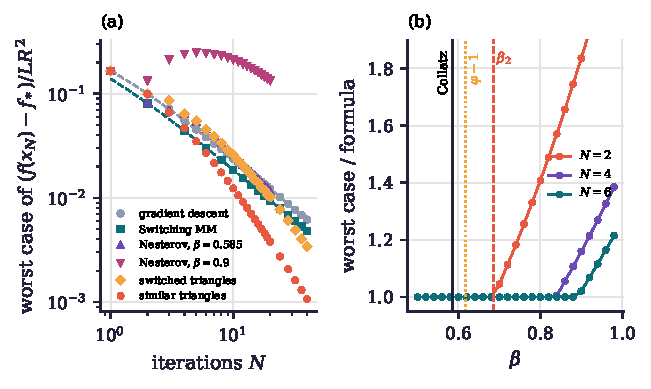
\includegraphics[width=\textwidth]{figures/ch5d_pep.pdf}
\caption{(a) Exact worst cases on smooth convex functions. Dashed lines:
$1/(4N+2)$ for gradient descent and $1/((4+2\beta)N+2)$ for Switching MM. Every
step Nesterov at $\beta=0.9$ has a large transient; similar triangles decay like
$1/N^2$, and the switched version overtakes Switching MM near $N=24$. (b) Worst
case of Switching MM divided by the conjectured formula, against $\beta$, for
$N=2,4,6$. Numerically the formula is exact up to $\beta_2$; the golden threshold of
\cref{thm:ch7b:smmrate} and the Collatz value are marked.}
\label{fig:ch7b:pep}
\end{figure}

Three things follow from the table. First, the ratio of the worst cases of
gradient descent and Switching MM tends to $1+\beta/2=1.29$, the same factor as
in \cref{thm:ch7b:smmrate}: the elementary three point proof captures the
right constant ratio, and only the common factor two is lost. Second, every
step Nesterov at the same $\beta=0.585$ is worse than gradient descent in the
worst case for $4\le N\le15$ and only slightly better for $16\le N\le20$, while Switching MM
is better at every even $N\ge2$, so on this measure the parity schedule is the better
way to spend a fixed momentum. This
is the reverse of the ordering in the average case experiments on random
quadratics of \cref{sec:ch7:experiments}, where every step injection was
faster; worst case and typical case answer different questions. Third, the
machine learning default $\beta=0.9$ has a worst case that rises to $0.251$ at
$N=5$ and is still eleven times that of gradient descent at $N=20$. Its transient
is the convex counterpart of the noise amplification $1/(1-\beta)=10$ of
\cref{chap:noise}.

In the language of long step gradient methods, Switching MM is a periodic step
size schedule $(1+\beta,1)$. Grimmer~\cite{grimmer2023} and Altschuler and
Parrilo~\cite{altschuler2024} showed that periodic and recursive long step
schedules beat gradient descent's constant and even its rate. The schedule of
Switching MM is the simplest member of that family, and
\cref{conj:ch7b:tight} would give its exact constant.

\section{Acceleration survives switching}\label{sec:ch7b:switching}

The energy of \cref{thm:ch7b:triangles} is robust in a way that matches the
switching results of \cref{chap:difference}.

\begin{proposition}[Every switching rule keeps the energy]\label{prop:ch7b:switch}
Consider any sequence of iterations each of which is either a similar
triangles step, as in \cref{sec:ch7b:triangles}, or a plain gradient step
$x^+=x-(s/L)\nabla f(x)$ with $0<s<2$, which leaves $z$ and $A$ unchanged. The
order of the two kinds of step may be arbitrary and may depend on the
iterates. Then the energy $E=A(f(x)-f_*)+\half\|z-x_*\|^2$ never increases,
and after $J$ similar triangles steps
\[
  f(x)-f_*\;\le\;\frac{2L\|x_0-x_*\|^2}{J^2}.
\]
In particular the switched method that alternates the two kinds of step,
starting with a similar triangles step, satisfies $f(x_N)-f_*\le8L\|x_0-x_*\|^2/N^2$.
\end{proposition}

\begin{proof}
A similar triangles step does not increase $E$ by \cref{thm:ch7b:triangles}.
A plain step with $s<2$ decreases $f$ by the descent lemma and leaves $A\ge0$
and $z$ unchanged, so it does not increase $E$ either. The bound follows from
$A\ge J^2/(4L)$ as before, and for the alternating method $J\ge N/2$.
\end{proof}

This is the convex analogue of \cref{cor:ch5b:anyswitch}, which says that on
quadratics, conditionally on \cref{conj:ch5b:transient}, every switching rule between the two steps of Switching MM is
stable. Here every switching rule between an accelerated step and a plain
one keeps the accelerated rate, measured in accelerated steps. The plain
steps are not wasted in practice, since they decrease $f$, but the energy
gives them no credit. Performance estimation shows that the worst case of the
alternating method approaches the energy bound $\|x_0-x_*\|^2/(2A)$, with $A$ its weight after the $J$ similar triangles steps, from below, reaching $0.72$ of it at
$N=20$ and $0.84$ at $N=40$, that it is no better than Switching MM up to
$N\approx22$, and that it overtakes Switching MM from $N=24$ on, as a $1/N^2$
rate must (\cref{tab:ch7b:pep}). If one wants a parity schedule with acceleration, this
is the way to build it: the momentum must be the shrinking ratio of the similar
triangles, not a fixed $\beta$.

\section{Does something similar happen for the Collatz map?}\label{sec:ch7b:collatz}

We now ask whether the Collatz map has a three point inequality. It has half
of one.

\subsection{The three point identity is exact}

Recall the linear majorizer of the logarithm from \cref{chap:lyapunov},
$\log y'\le\log y+(y'-y)/y$ (\cref{prop:mmdescent}). Its gap is a Bregman
divergence: for $h=-\log$,
\[
  \log y'=\log y+\frac{y'-y}y-D\Bigl(\frac{y'}y\Bigr),\qquad D(t)=t-1-\log t\ \ge0,
\]
and $D(t)=D_h(t,1)$ is the Itakura and Saito divergence~\cite{banerjee2005}.
Apply this along a Syracuse orbit $y_{i+1}=S(y_i)$ and write
$M_i=y_{i+1}/y_i=(3+1/y_i)/2^{k_i}$ with $k_i=\vt(3y_i+1)$.

\begin{proposition}[Bregman decomposition of an orbit]\label{prop:ch7b:bregman}
For every odd $y_0$ and every $N$,
\[
  \log y_N-\log y_0=\sum_{i<N}(M_i-1)\;-\;\sum_{i<N}D(M_i).
\]
Under the stride model of \cref{chap:stochastic}, in which
$M=3/2^k$ with $k$ Geometric$(\half)$, the first sum is a martingale,
$\E M=1$, and the expected dissipation per step equals the drift exactly,
$\E D(M)=-\E\log M=\log(4/3)$.
\end{proposition}

\begin{proof}
The identity is the displayed gap formula summed over the orbit. In the
model $\E M=3\sum_k4^{-k}=1$ and $\E\log M=\log3-2\log2$, so
$\E D(M)=\E M-1-\E\log M=\log(4/3)$.
\end{proof}

This is exactly the structure of the energy proofs above: an increment equal to
a linear term minus a nonnegative divergence. The drift of $\log y$ that the
book has used since \cref{chap:stochastic}, $\log(3/4)$ per Syracuse step, is
in this language minus the expected Bregman dissipation, and the linear term is the additive companion of
the multiplicative martingale of \cref{thm:martingale}, a martingale for the same reason, $\E M=1$. The decomposition holds on real
orbits as well as in the model. Over $400$ orbits from random odd starting
values of $3000$ bits, $2\,898\,459$ Syracuse steps in all, the mean dissipation
per step is $0.28718$ against $\log(4/3)=0.28768$, the mean of $M_i-1$ is
$0.00034$ against $0$, and the variance of $M_i$ is $0.28543$ against the model
value $2/7=0.28571$ (script \texttt{ch5d\_collatz\_bregman.py}).
\Cref{fig:ch7b:collatz}(a) shows the three terms along one orbit: the
martingale part wanders near zero, and the descent of $\log y$ is all
dissipation.

\begin{figure}[t]
\centering
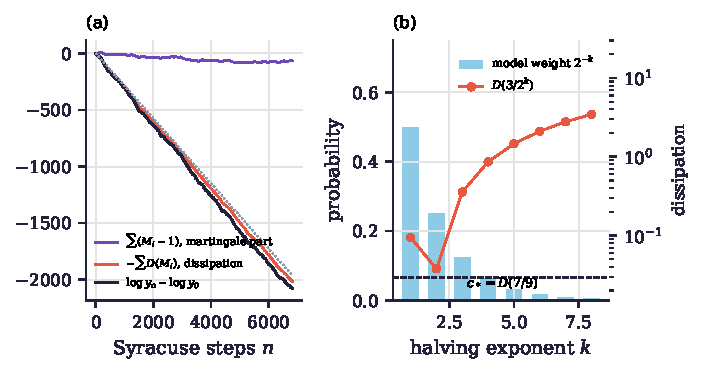
\includegraphics[width=\textwidth]{figures/ch5d_collatz.pdf}
\caption{(a) The Bregman decomposition along the Syracuse orbit of a random
$3000$ bit odd integer: the martingale part $\sum(M_i-1)$, the dissipation
$-\sum D(M_i)$, and their sum $\log y_n-\log y_0$, with the model slope
$-\log(4/3)$ dotted. (b) The dissipation $D(3/2^k)$ of each halving exponent
(log scale, right) and its model weight $2^{-k}$ (left); the dashed line is the
uniform lower bound $c_*$ of \cref{prop:ch7b:dissipation}.}
\label{fig:ch7b:collatz}
\end{figure}

\subsection{Uniform dissipation}

The dissipation is not only positive on average. In the model every multiplier
$3/2^k$ has $D(3/2^k)\ge D(\tfrac34)$, and the real map, with its correction
$1/y$, dissipates a fixed amount at every single step as well.

\begin{proposition}[Uniform dissipation]\label{prop:ch7b:dissipation}
For every odd $y\ge3$,
\[
  D\Bigl(\frac{S(y)}y\Bigr)\;\ge\;c_*=D\bigl(\tfrac79\bigr)=\log\tfrac97-\tfrac29=0.029092\ldots,
\]
with equality only at $y=9$, and $\liminf_{y\to\infty}D(S(y)/y)=D(\tfrac34)=\log\tfrac43-\tfrac14=0.037682\ldots$.
\end{proposition}

\begin{proof}
The function $D$ is convex with its minimum $0$ at $t=1$, decreasing on
$(0,1)$ and increasing on $(1,\infty)$. Write $M=(3+1/y)/2^k$. If $k=1$ then
$M>3/2$ and $D(M)>D(3/2)=\half-\log\tfrac32=0.0945$. If $k\ge3$ then
$M\le(3+\tfrac13)/8=\tfrac5{12}$ and $D(M)\ge D(\tfrac5{12})=0.292$. If $k=2$
then $3y+1\equiv4\pmod8$, so $y\equiv1\pmod8$ and $y\ge9$; then
$\tfrac34<M\le(3+\tfrac19)/4=\tfrac79$, and since $D$ decreases on $(0,1)$,
$D(M)\ge D(\tfrac79)$ with equality only at $y=9$. As $y\to\infty$ along
$y\equiv1\pmod8$ with $k=2$, $M\downarrow\tfrac34$, and the other cases stay
above $D(3/2)>D(3/4)$.
\end{proof}

\begin{corollary}[The martingale part must outrun the dissipation]\label{cor:ch7b:outrun}
If the Syracuse orbit of $y_0$ is unbounded, then
\[
  \limsup_{N\to\infty}\frac1N\sum_{i<N}M_i\;\ge\;1+D(\tfrac34)=1.0377.
\]
If the orbit lies on a nontrivial cycle of $r$ odd elements, then the mean of
the $r$ ratios $M_i$ around the cycle is at least $1+c_*$.
\end{corollary}

\begin{proof}
An unbounded orbit tends to infinity (\cref{lem:ch9:infinity}), so
$D(M_i)\ge D(\tfrac34)-\varepsilon$ for all large $i$, and $\log y_N>\log y_0$
for infinitely many $N$. For those $N$, \cref{prop:ch7b:bregman} gives
$\sum_{i<N}(M_i-1)>\sum_{i<N}D(M_i)$. Dividing by $N$ and letting $\varepsilon\to0$
gives the first claim. On a cycle $\log y_r=\log y_0$, so
$\sum(M_i-1)=\sum D(M_i)\ge rc_*$.
\end{proof}

We should say plainly that these are not new constraints. On a long cycle the
exponents $k_i$ are integers with mean $s/r$ close to $\lt$, and since $2^{-k}$
is convex the mean of $3/2^{k_i}$ is then at least about
$3(3-\lt)/4=1.061$, which is stronger than $1+c_*$; the same convexity argument
applies to divergent orbits through \cref{cor:ch9:freq}. The Bregman
decomposition reorganizes what integrality and the Ces\`aro identity already
give. Its value is that it identifies which term carries the difficulty.

\subsection{What is missing}

The three point inequality of \cref{lem:ch7b:inequality} has two ingredients,
the identity and the variational inequality of a convex minimization. The
Collatz map has the first, exactly, in \cref{prop:ch7b:bregman}, together with
a uniform dissipation that the convex setting supplies only through the term
$D_h(z^+,z)$. It does not have the second. In an MM method the linear term
$\langle\nabla f(z),z^+-u\rangle$ is controlled because $z^+$ was chosen to
minimize the surrogate over a convex set, and the variational inequality
bounds it by the distance terms. In the Collatz map the linear term is
$\sum(M_i-1)$, and nothing controls it: the successor of $y$ is dictated by the
parity of $y$, not chosen to minimize anything. Even if one views the step as a
minimization over a finite set of candidate successors, as in
\cref{chap:mmcollatz}, a finite set carries no variational inequality, and the
three point inequality has nothing to stand on.

In this language the divergence half of the conjecture is a three point
inequality along orbits: for every $y_0$ there is a constant $C(y_0)$ with
\[
  \sum_{i<N}(M_i-1)\;\le\;\sum_{i<N}D(M_i)+C(y_0)\qquad\text{for all }N.
\]
This is equivalent to the boundedness of the orbit, so it is no easier. But it
locates the difficulty precisely. The dissipation is uniform and positive, and
the martingale part is the only term without a sign. In the model it has mean
zero and variance $2/7$ per step, so it grows like $\sqrt N$ while the
dissipation grows like $N$, and the inequality holds with room to spare. Along
one deterministic orbit, controlling the martingale part is the same problem
as controlling the Ces\`aro averages of \cref{chap:divergence}, and it is the
problem no method yet solves.

\section{Summary}\label{sec:ch7b:summary}

\Cref{tab:ch7b:summary} sets the four settings of this chapter side by side.

\begin{table}[ht]
\centering\small
\setlength{\tabcolsep}{3pt}
\caption{The three point structure in four settings.}
\label{tab:ch7b:summary}
\begin{tabular}{@{}>{\raggedright\arraybackslash}p{0.20\textwidth}>{\raggedright\arraybackslash}p{0.17\textwidth}>{\raggedright\arraybackslash}p{0.17\textwidth}>{\raggedright\arraybackslash}p{0.19\textwidth}>{\raggedright\arraybackslash}p{0.19\textwidth}@{}}
\toprule
 & MM step & similar triangles & Switching MM & Collatz map \\
\midrule
three point identity & yes & yes & yes & yes, exactly \\
dissipation & $D_h(z^+,z)$ & $\half\|z^+-z\|^2$, cancelled & cocoercivity & uniform, $c_*=0.029$ \\
optimality of the step & yes & yes & yes, if $1+\beta\le\varphi$ & no \\
growth of the weights & $1$ per step & $\approx k/(2L)$ & $2+\beta$ per pair & none \\
rate & $1/N$ & $1/N^2$ & $1/N$, constant $1+\beta/2$ better & open \\
\bottomrule
\end{tabular}
\end{table}

The three point inequality is the engine of every convergence proof in
convex optimization, and the similar triangles are what make it accelerate.
Pressed on Switching MM it yields a new convex rate with the exact constant
ratio $1+\beta/2$ to gradient descent, a golden ratio condition, and a
conjectured exact worst case that generalizes the theorem of Drori and
Teboulle. Pressed on the Collatz map it yields an exact identity, a uniform
dissipation and a clean statement of what is missing: the optimality of the
step, which a map that does not choose its successor cannot have.

\section*{Notes}

The three point identity for Bregman divergences is due to Chen and
Teboulle~\cite{chen1993}. The method of similar triangles is from Gasnikov and
Nesterov~\cite{gasnikov2018}; Nesterov's method itself is from~\cite{nesterov1983},
the estimate sequence form from~\cite{nesterov2004}, the accelerated proximal
method from Beck and Teboulle~\cite{beck2009}, and a unified analysis of the
variants from Tseng~\cite{tseng2008}. Relative smoothness is due to Bauschke,
Bolte and Teboulle~\cite{bauschke2017} and to Lu, Freund and Nesterov~\cite{lu2018}.
The tight worst case $1/(4N+2)$ of gradient descent is due to Drori and
Teboulle~\cite{drori2014}, and the interpolation conditions behind the
performance estimation programs to Taylor, Hendrickx and Glineur~\cite{taylor2017}.
Long step schedules are studied by Grimmer~\cite{grimmer2023} and by Altschuler
and Parrilo~\cite{altschuler2024}. The Itakura and Saito divergence as a
Bregman divergence is discussed by Banerjee, Merugu, Dhillon and
Ghosh~\cite{banerjee2005}.

\Cref{lem:ch7b:identity}, \cref{lem:ch7b:inequality}, \cref{thm:ch7b:mm} and
\cref{thm:ch7b:triangles} are classical; the proofs are given in the form used
here. \Cref{thm:ch7b:smmrate}, \cref{conj:ch7b:tight} with the threshold
$\beta_2$, \cref{prop:ch7b:switch}, the performance estimation results of
\cref{tab:ch7b:pep}, \cref{prop:ch7b:bregman} in the form stated,
\cref{prop:ch7b:dissipation} and \cref{cor:ch7b:outrun} are new in this book.
\begin{sloppypar}
The scripts are \texttt{ch5d\_pep.py}, \texttt{ch5d\_golden.py},
\texttt{ch5d\_threshold.py}, \texttt{ch5d\_cross.py},
\texttt{ch5d\_collatz\_bregman.py} and \texttt{ch5d\_figures.py}.
\end{sloppypar}

\section*{Exercises}

\begin{exercise}
Prove \cref{lem:ch7b:identity} for a general Bregman divergence, and check that
for $h=-\log$ on the positive reals it gives the identity
$D(a,c)=D(a,b)+D(b,c)+(a-b)(1/c-1/b)$ for the Itakura and Saito divergence
$D(a,b)=a/b-1-\log(a/b)$.
\end{exercise}

\begin{exercise}
Let $h(x)=\sum_ix_i\log x_i$ on the probability simplex. Show that the MM step
of \cref{thm:ch7b:mm} is the exponentiated gradient update
$z^+_i\propto z_i\exp(-\nabla_if(z)/L)$, and state the rate the theorem gives
when $f$ is $L$ smooth relative to the entropy.
\end{exercise}

\begin{exercise}
In the method of similar triangles show that $\tau_k=a_{k+1}/A_{k+1}$ satisfies
$\tau_k\sim2/k$, and that in momentum form $x_{k+1}=y_k-\nabla f(y_k)/L$,
$y_{k+1}=x_{k+1}+\gamma_k(x_{k+1}-x_k)$ the coefficient is
$\gamma_k=\tau_{k+1}(1-\tau_k)/\tau_k$. Compare with Nesterov's $(k-1)/(k+2)$.
\end{exercise}

\begin{exercise}
Show that $s(s^2-s-1)\le0$ for $0<s\le\varphi$ and compute the margin at
$s=\lt$. Then repeat the proof of \cref{thm:ch7b:smmrate} for gradient descent
with a constant step $s/L$, $0<s\le\varphi$, and show that
$f(x_N)-f_*\le LR^2/(2sN)$. Deduce that \eqref{eq:ch7b:pair} is the sum of two one step inequalities, and explain why
\eqref{eq:ch7b:unit}, which treats a step as an MM step, needs $s\le1$.
\end{exercise}

\begin{exercise}
List the odd $y<200$ for which $D(S(y)/y)<D(\tfrac34)$, and explain from the
proof of \cref{prop:ch7b:dissipation} why every one of them is congruent to $1$
modulo $8$.
\end{exercise}


\renewcommand{\partimagehook}{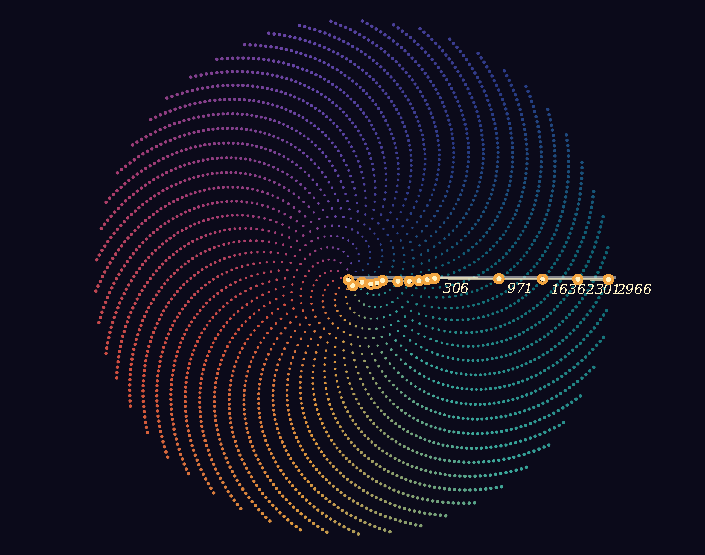
\includegraphics[width=0.92\textwidth]{figures/art_part3}\par\vspace{8pt}{\normalsize\upshape\itshape The sunflower of $r\log_23$ modulo $1$ for $r\le3000$: angle is the fractional part, radius $\sqrt r$; the gold rings are the rungs of the one sided ladder that control every cycle bound.\par}}
\part{Cycles and Divergence}
\chapter{Cycles and Continued Fractions}\label{chap:cycles}

The Collatz conjecture\index{Collatz conjecture} asserts two things at once: no orbit of a positive
integer escapes to infinity, and no orbit settles into a cycle other than
$1\mapsto4\mapsto2\mapsto1$. \Cref{chap:intro} called these the divergence
half and the cycle half. The two halves are very different in character. The
divergence half is a statement about the long run behaviour of a single
orbit, and all the probabilistic machinery of the earlier chapters bears on it
only through ensembles. The cycle half is much more rigid. A cycle is a finite
object, it satisfies an exact multiplicative identity, and that identity turns
the question into one about how well the number $\lt$ can be approximated by
rationals.

This chapter develops that reduction completely. We begin with the cycles that
do exist, on the negative integers\index{negative cycles} and on the rationals with odd denominator,
because they show that the cycle identity\index{cycle identity} is not vacuous. We then prove the
identity and its consequence, an upper bound on the least element of a cycle
in terms of the one sided distance from $r\lt$ up to the next integer, where
$r$ is the number of odd elements. To exploit it we need continued fractions\index{continued fraction},
and we give a primer that is complete in itself, including the classical
theorem identifying the best one sided approximations\index{one sided approximation} with the intermediate
fractions of one parity~\cite[Theorem~4.5(ii)]{hancl2019}. The heart of the chapter is a short \emph{mediant
lemma}, a self contained proof of a classical fact, which shows that the first value of $r$ not excluded
by a given verification range\index{verification range} must be a best one sided approximation. This
makes the search for the sharp cycle bound short and rigorous: with the
verification range $2^{68}$, and equally with the current range $2^{71}$, every nontrivial cycle has at least
$72\,057\,431\,991$ odd elements. We compare this with the cruder bounds one
obtains without the lemma, place it in the literature (where sharper
numerical bounds exist and where we claim no priority), and then prove that
no Diophantine\index{Diophantine approximation} argument of this kind can finish the job, a point that Halbeisen\index{Halbeisen, L.} and Hungerb\"uhler\index{Hungerbuhler, N.@Hungerb\"uhler, N.}~\cite[\S5]{halbeisen1997} made earlier in another form (\cref{rem:attribution}): for every
verification range infinitely many $r$ survive. What is missing is arithmetic
information about the parity word, and a window lemma\index{window lemma} makes precise how much
would suffice. We also give an exact integer certificate\index{certificate} for the sharp bound.

Two further sections connect the chapter to recent work. The first treats a
sibling problem of Erd\H{o}s, settled in 2026 by an automated prover, in which
good rational approximations to $\lt$ play the opposite role. The second describes a
small library of machine checked statements in the Lean\index{Lean} proof assistant and
the path from it to a fully verified cycle bound.

Throughout, $\theta=\lt=1.584963\ldots$, $\log$ is the natural logarithm, and we use the three maps of
\cref{def:maps}: the standard map\index{standard map} $T_0$, the accelerated map\index{accelerated map} $T$ and the
Syracuse map\index{Syracuse map} $S$.

\section{The cycles that exist}\label{sec:ch8:exist}

\subsection{The trivial cycle}

The orbit of $1$ is periodic under all three maps: $1\mapsto4\mapsto2\mapsto1$
under $T_0$, $1\mapsto2\mapsto1$ under $T$, and $S(1)=1$. It has one odd
element and two halvings, so in the notation used below $r=1$ and $s=2$, with
period $r+s=3$ under $T_0$, period $s=2$ under $T$ and period $r=1$ under $S$.
The conjecture is that every positive integer eventually enters this cycle;
the cycle half asks only that there be no other.

\subsection{Cycles on the negative integers}

The maps $T_0$, $T$ and $S$ make sense on all of $\Z$, and on the negative
integers there are several cycles. Under $n\mapsto-n$ the standard map\index{standard map} on the
negative integers\index{negative cycles} becomes the map $n\mapsto n/2$ for even $n$ and
$n\mapsto3n-1$ for odd $n$ on the positive integers, the so called $3x-1$
problem, so these cycles are cycles of that problem in disguise. We ran $T_0$
from every starting value $n=-1,-2,\dots,-10^{6}$ and recorded the cycle that
each orbit enters (script \texttt{ch08\_negative.py}). Exactly three cycles
occur, and every one of the $10^6$ starting values falls into one of them.

\begin{table}[ht]
\centering
\caption{The cycles of $T_0$ entered by orbits of $n=-1,\dots,-10^{6}$. Here
$r$ is the number of odd elements and $s$ the number of halvings, so the
period under $T_0$ is $r+s$. The last column counts the starting values that
reach the cycle.}
\label{tab:ch8:negative}
\begin{tabular}{@{}lrrrr@{}}
\toprule
odd elements & $r$ & $s$ & $r+s$ & orbits \\
\midrule
$-1$ & $1$ & $1$ & $2$ & $327\,679$ \\
$-5,-7$ & $2$ & $3$ & $5$ & $323\,351$ \\
$-17,-25,-37,-55,-41,-61,-91$ & $7$ & $11$ & $18$ & $348\,970$ \\
\bottomrule
\end{tabular}
\end{table}

The second cycle is $-5\mapsto-14\mapsto-7\mapsto-20\mapsto-10\mapsto-5$ and
the third, of period $18$ under $T_0$, starts
$-17\mapsto-50\mapsto-25\mapsto-74\mapsto\cdots$. In each case the product of
the factors $3+1/x$ over the odd elements $x$ is an exact power of two: $2$
for the first cycle, $(3-\tfrac15)(3-\tfrac17)=8$ for the second, and $2^{11}$
for the third (we checked the last in exact rational arithmetic). This is the
cycle identity\index{cycle identity} of \cref{lem:cycleid} below. Because the elements are negative
the factors are less than $3$, so $2^s<3^r$, that is, $s<r\theta$: indeed
$3<2\theta=3.17$ and $11<7\theta=11.09$. For positive cycles the inequality
goes the other way, and that change of sign is the whole difficulty. The
negative cycles exist because $2^s$ may undershoot $3^r$ by a little; a
positive cycle would need $2^s$ to overshoot $3^r$ by very little, and the
rest of this chapter quantifies how little.

\subsection{Rational cycles}

Solving the affine identity \eqref{eq:ch2:affine} for a point that returns to itself, as in the proof of \cref{cor:ch2:cycle}, gives, for any parity word $w$ of length $k$ with $m$
ones, the number
\[
  n(w)=\frac{c(w)}{2^k-3^m},
\]
where $c(w)$ is the sum \eqref{eq:ch2:cexplicit}. The identity
\eqref{eq:ch2:affine} holds in the ring of rationals with odd denominator,
in which parity is the parity of the numerator, and reading it backwards shows
that $n(w)$ is a periodic point of $T$ with parity word $w$, repeated. For
example $w=(1,0,0)$ has $c=1$ and $n=1/(8-3)=1/5$, and indeed
$\tfrac15\mapsto\tfrac45\mapsto\tfrac25\mapsto\tfrac15$. Every word thus gives
a rational cycle\index{rational cycles}, and the integer cycles are exactly the words for which
$2^k-3^m$ divides $c(w)$. Lagarias\index{Lagarias, J. C.}~\cite{lagarias1990} studied the set of
these rational cycles systematically, organizing them by denominator; for a
denominator $d$ coprime to $6$ they correspond to the integer cycles, with elements prime to $d$, of the map that sends $x$ to $(3x+d)/2$ for odd $x$ and to $x/2$ for even $x$, and he showed, among other things, that cycles exist for many denominators. We shall not need this theory. Its lesson for us is that
there is no shortage of periodic parity words; what is rare is the
divisibility that makes $n(w)$ an integer, and for positive integers the
inequality $3^m<2^k$ of \cref{cor:ch2:cycle} combined with the size of the
elements is the only handle we have.

\section{The cycle identity}\label{sec:ch8:identity}

It is most convenient to describe a cycle by its odd elements. Suppose $S$ has
a cycle of positive odd integers $x_1,\dots,x_r$, with $x_{i+1}=S(x_i)$
(indices modulo $r$), and let $k_i=\vt(3x_i+1)\geq1$ be the halving exponents,
so that
\begin{equation}\label{eq:ch8:stride}
  x_{i+1}=\frac{3x_i+1}{2^{k_i}} .
\end{equation}
Put $s=\sum_i k_i$, the total number of halvings in one turn of the cycle.

\begin{lemma}[Cycle identity]\label{lem:cycleid}
For a cycle of $S$ as above,
\begin{equation}\label{eq:ch8:prod}
  \prod_{i=1}^{r}\Bigl(3+\frac{1}{x_i}\Bigr)=2^{s},
\end{equation}
and therefore, writing $M=\min_i x_i$ for the least element,
\begin{equation}\label{eq:ch8:Lambda}
  \Lambda:=s\log2-r\log3=\sum_{i=1}^{r}\log\Bigl(1+\frac{1}{3x_i}\Bigr)
  \in\Bigl(0,\ \frac{r}{3M}\Bigr).
\end{equation}
Equivalently,
\begin{equation}\label{eq:ch8:theta}
  0<s-r\theta<\frac{r}{3M\log2},
\end{equation}
and in particular $s/r>\theta$.
\end{lemma}

\begin{proof}
Multiply the $r$ relations \eqref{eq:ch8:stride} around the cycle. The
product of the left sides is $\prod_ix_i$ and the product of the right sides
is $\prod_i(3x_i+1)/2^{s}$, so $2^s=\prod_i(3x_i+1)/x_i$, which is
\eqref{eq:ch8:prod}. Taking logarithms and writing
$\log(3+1/x_i)=\log3+\log(1+1/(3x_i))$ gives the middle expression in
\eqref{eq:ch8:Lambda}. Each summand is positive, so $\Lambda>0$, and since
$\log(1+u)<u$ for $u>0$ and $1/(3x_i)\leq1/(3M)$, we get
$\Lambda<r/(3M)$.
Dividing by $\log2$ gives \eqref{eq:ch8:theta}.
\end{proof}

The same identity can be read off from the affine form of
\cref{prop:ch2:affine}. If $n$ is an element of a cycle of $T$ of length $k$
with $m$ odd steps, then \eqref{eq:ch2:product} with $T^{(k)}(n)=n$ says that
$2^k/3^m$ is the product of $1+1/(3y)$ over the odd elements $y$ of the cycle.
That is \eqref{eq:ch8:prod} with $m=r$ and $k=s$.

\begin{remark}[A pitfall: bookkeeping under the accelerated map]\label{rem:ch8:bookkeeping}
The three maps count the same cycle differently, and it is easy to mix the
counts. Under the Syracuse map\index{Syracuse map} $S$ the cycle has period $r$. Under the
accelerated map\index{accelerated map} $T$ each odd step already contains one halving, so the cycle
has $s$ steps in all, of which $r$ are odd and $s-r$ are even. Under the
standard map\index{standard map} $T_0$ every halving is a separate step and so is every tripling,
so the period is $r+s$. For the trivial cycle these are $1$, $2$ and $3$.
The linear form can be written either as $s\log2-r\log3$ or as
$s'\log2-r\log(3/2)$ with $s'=s-r$ the number of even steps of $T$, and the
two are equal. The danger lies in the derived quantities. If one works with
$s'$ and then reports $s'$, or $s$, as ``the period'' of the cycle, the
answer is wrong for $T_0$, whose period is $r+s=2r+s'$. And the feasibility
condition must be stated for the right pair: it is $s/r>\theta$, equivalently
$s'/r>\theta-1=\log_2(3/2)$, together with the constraint $s'\geq0$ that
comes from $k_i\geq1$. Lower bounds on cycle length in the literature are
quoted in all three conventions, and comparisons between them are meaningless
unless the convention is fixed. In this chapter $r$ is the number of odd
elements and $s$ the number of halvings, so that a cycle has $r$ steps of
$S$, $s$ steps of $T$ (of which $r$ are odd) and $r+s$ steps of $T_0$.
\end{remark}

For fixed $r$ the strongest conclusion comes from the smallest admissible
$\Lambda$. Since $s$ must be an integer with $s>r\theta$, we have
$s\geq\lceil r\theta\rceil$ and so
\begin{equation}\label{eq:ch8:Lambdar}
  \Lambda\geq\Lambda_r:=\delta(r)\log2,\qquad
  \delta(r):=\lceil r\theta\rceil-r\theta\in(0,1).
\end{equation}
(The value $\delta(r)$ is never $0$ because $\theta$ is irrational: $2^s=3^r$
is impossible for $r\geq1$.) Combining with \eqref{eq:ch8:Lambda} gives the
basic inequality of the chapter:
\begin{equation}\label{eq:ch8:maxM}
  M<\frac{r}{3\Lambda_r}=\frac{r}{3\,\delta(r)\log2}=:F(r).
\end{equation}
The function $F$ depends only on $\theta$ and $r$. A cycle with $r$ odd
elements must have its least element below $F(r)$. On the other hand, if
every positive integer up to some bound reaches $1$, then every element of a
nontrivial cycle exceeds that bound. These two facts squeeze the cycle.

\begin{definition}[Verification range and exclusion]\label{def:ch8:excl}
We say that $X$ is a \emph{verified range\index{verification range}} if every element of every
nontrivial cycle of positive integers is at least $X$; this holds, for
example, if every positive integer $n<X$ is known to reach $1$. Given $X$, put
$\varepsilon=\varepsilon(X)=1/(3X\log2)$ and say that $r\geq1$ is
\emph{excluded} if $\delta(r)\geq r\varepsilon$, equivalently $F(r)\leq X$.
\end{definition}

\begin{corollary}\label{cor:ch8:excl}
If $X$ is a verified range, then a nontrivial cycle with $r$ odd elements
satisfies $\delta(r)<r\varepsilon$, so $r$ is not excluded.
\end{corollary}

\begin{proof}
By \eqref{eq:ch8:theta}, $\delta(r)\leq s-r\theta<r/(3M\log2)\leq
r/(3X\log2)=r\varepsilon$.
\end{proof}

By Ba\v{r}ina\index{Barina, D.@Ba\v{r}ina, D.}~\cite{barina2021}, every positive integer below $2^{68}$
reaches $1$, so $X=2^{68}=2.95148\times10^{20}$ is a verified range. Ba\v{r}ina~\cite{barina2025} has since extended the verification to $2^{71}$; we keep $X=2^{68}$ in the examples, and \cref{sec:ch8:bound} shows that the larger range gives the same sharp bound. The
question is now purely arithmetic: which $r$ satisfy $\delta(r)<r\varepsilon$?
The inequality says that $r\theta$ lies just \emph{below} an integer, closer
than $r\varepsilon$. To find all such $r$ we need the theory of rational
approximation, and specifically its one sided form.

\section{A primer on continued fractions}\label{sec:ch8:cf}

This section collects what we need about continued fractions\index{continued fraction}, with proofs.
The material is classical; good references are the books of
Khinchin\index{Khinchin, A. Ya.}~\cite{khinchin1964}, Hardy\index{Hardy, G. H.} and Wright\index{Wright, E. M.}~\cite{hardywright2008} and
Rockett\index{Rockett, A. M.} and Sz\"usz\index{Szusz, P.@Sz\"usz, P.}~\cite{rockett1992}, the last of which treats one sided
approximation in detail.

\subsection{Convergents and their recurrences}

Let $\theta>0$ be irrational. Define $\theta_0=\theta$ and, recursively,
$a_k=\lfloor\theta_k\rfloor$ and $\theta_{k+1}=1/(\theta_k-a_k)>1$. Then
$a_0\geq0$, $a_k\geq1$ for $k\geq1$, and for every $k$
\[
  \theta=a_0+\cfrac{1}{a_1+\cfrac{1}{\ddots+\cfrac{1}{a_k+\cfrac{1}{\theta_{k+1}}}}}
  =:[a_0;a_1,\dots,a_k,\theta_{k+1}].
\]
The numbers $a_k$ are the \emph{partial quotients} and $\theta_k$ the
\emph{complete quotients}. Define integers $p_k,q_k$ by
\begin{equation}\label{eq:ch8:recur}
  \begin{gathered}
  p_k=a_kp_{k-1}+p_{k-2},\qquad q_k=a_kq_{k-1}+q_{k-2},\\
  p_{-2}=0,\quad p_{-1}=1,\quad q_{-2}=1,\quad q_{-1}=0 .
  \end{gathered}
\end{equation}
Thus $p_0=a_0$, $q_0=1$, $q_1=a_1$, and $1=q_0\leq q_1<q_2<q_3<\cdots$. The
fractions $p_k/q_k$ are the \emph{convergents\index{convergent}}.

\begin{lemma}[Basic identities]\label{lem:ch8:basic}
For every $k\geq0$:
\begin{enumerate}[label=(\roman*),leftmargin=2em]
\item $\begin{pmatrix}a_0&1\\1&0\end{pmatrix}\cdots
  \begin{pmatrix}a_k&1\\1&0\end{pmatrix}
  =\begin{pmatrix}p_k&p_{k-1}\\q_k&q_{k-1}\end{pmatrix}$;
\item $p_kq_{k-1}-p_{k-1}q_k=(-1)^{k-1}$, and this also holds for $k=-1$;
\item $\theta=\dfrac{\theta_{k+1}p_k+p_{k-1}}{\theta_{k+1}q_k+q_{k-1}}$;
\item $q_k\theta-p_k=\dfrac{(-1)^k}{\theta_{k+1}q_k+q_{k-1}}$. In particular
  $p_k/q_k<\theta$ for even $k$ and $p_k/q_k>\theta$ for odd $k$, and the
  error $\varepsilon_k:=|q_k\theta-p_k|$ satisfies
  \[
    \frac{1}{q_{k+1}+q_k}<\varepsilon_k<\frac{1}{q_{k+1}};
  \]
\item $\varepsilon_{k+1}=\varepsilon_{k-1}-a_{k+1}\varepsilon_k$, where
  $\varepsilon_{-1}=|q_{-1}\theta-p_{-1}|=1$.
\end{enumerate}
\end{lemma}

\begin{proof}
(i) is induction on $k$ using \eqref{eq:ch8:recur}, since multiplying the
matrix
$\bigl(\begin{smallmatrix}p_{k-1}&p_{k-2}\\q_{k-1}&q_{k-2}\end{smallmatrix}\bigr)$
on the right by
$\bigl(\begin{smallmatrix}a_k&1\\1&0\end{smallmatrix}\bigr)$ gives
$\bigl(\begin{smallmatrix}p_k&p_{k-1}\\q_k&q_{k-1}\end{smallmatrix}\bigr)$.
(ii) Take determinants in (i): each factor has determinant $-1$; for $k=-1$,
$p_{-1}q_{-2}-p_{-2}q_{-1}=1$.
(iii) The matrix
$\bigl(\begin{smallmatrix}a&1\\1&0\end{smallmatrix}\bigr)$ acts on $t$ as the
M\"obius map $t\mapsto a+1/t$, and composition of M\"obius maps corresponds to
matrix multiplication, so by (i) the map
$t\mapsto[a_0;a_1,\dots,a_k,t]$ is
$t\mapsto(tp_k+p_{k-1})/(tq_k+q_{k-1})$; put $t=\theta_{k+1}$.
(iv) From (iii),
$q_k\theta-p_k=(q_kp_{k-1}-p_kq_{k-1})/(\theta_{k+1}q_k+q_{k-1})$, and the
numerator is $(-1)^k$ by (ii). Since $a_{k+1}<\theta_{k+1}<a_{k+1}+1$, the
denominator lies strictly between $a_{k+1}q_k+q_{k-1}=q_{k+1}$ and
$q_{k+1}+q_k$.
(v) Multiply the recurrence \eqref{eq:ch8:recur} at index $k+1$ by $\theta$
and subtract: $q_{k+1}\theta-p_{k+1}=a_{k+1}(q_k\theta-p_k)+
(q_{k-1}\theta-p_{k-1})$. By (iv), and for $k=0$ by $q_{-1}\theta-p_{-1}=-1$,
the outer two terms have the same sign and the middle one the opposite sign,
which gives the stated relation between absolute values.
\end{proof}

\subsection{Best approximation}

Write $\|t\|$ for the distance from $t$ to the nearest integer. The next
theorem, due in essence to Lagrange\index{Lagrange, J. L.}, is the best approximation property: no
denominator smaller than $q_{k+1}$ approximates $\theta$ better than $q_k$.

\begin{theorem}[Best approximation]\label{thm:ch8:best}
Let $k\geq0$, $1\leq r<q_{k+1}$ and $s\in\Z$. Then
$|r\theta-s|\geq\varepsilon_k$. In particular $\|r\theta\|\geq\varepsilon_k
\geq\|q_k\theta\|$.
\end{theorem}

\begin{proof}
By \cref{lem:ch8:basic}(ii) the matrix
$\bigl(\begin{smallmatrix}p_k&p_{k+1}\\q_k&q_{k+1}\end{smallmatrix}\bigr)$
has determinant $\pm1$, so there are integers $x,y$ with $s=xp_k+yp_{k+1}$ and
$r=xq_k+yq_{k+1}$. Then
$r\theta-s=x(q_k\theta-p_k)+y(q_{k+1}\theta-p_{k+1})$. If $y=0$ then
$r=xq_k$ with $x\geq1$, and $|r\theta-s|=x\varepsilon_k\geq\varepsilon_k$. If
$x=0$ then $r=yq_{k+1}$, which is impossible for $1\leq r<q_{k+1}$. If $x$
and $y$ are both positive then $r\geq q_k+q_{k+1}>q_{k+1}$, and if both are
negative then $r<0$; both are impossible. So $x$ and $y$ are nonzero with
opposite signs. Since $q_k\theta-p_k$ and $q_{k+1}\theta-p_{k+1}$ also have
opposite signs, by \cref{lem:ch8:basic}(iv), the two terms
$x(q_k\theta-p_k)$ and $y(q_{k+1}\theta-p_{k+1})$ have the same sign, and
$|r\theta-s|\geq|x|\varepsilon_k\geq\varepsilon_k$.
\end{proof}

\subsection{Intermediate fractions}

Between two convergents\index{convergent} on the same side of $\theta$ one may interpolate. For
$k\geq0$ and $0\leq j\leq a_{k+1}$ define
\begin{equation}\label{eq:ch8:rung}
  u_{k,j}=q_{k-1}+jq_k,\qquad P_{k,j}=p_{k-1}+jp_k .
\end{equation}
For $j=0$ this is the convergent $p_{k-1}/q_{k-1}$, for $j=a_{k+1}$ it is
$p_{k+1}/q_{k+1}$, and the fractions $P_{k,j}/u_{k,j}$ with $0<j<a_{k+1}$
are the \emph{intermediate fractions\index{semiconvergent}}, or \emph{semiconvergents}. We call the
denominators $u_{k,j}$ the \emph{rungs} of the \emph{semiconvergent ladder}:
the ladder from $q_{k-1}$ to $q_{k+1}$ climbs in steps of $q_k$,
\[
  q_{k-1},\ q_{k-1}+q_k,\ q_{k-1}+2q_k,\ \dots,\ q_{k-1}+a_{k+1}q_k=q_{k+1}.
\]
By \cref{lem:ch8:basic}(iv) and (v),
\begin{equation}\label{eq:ch8:rungerr}
  P_{k,j}-u_{k,j}\theta=(-1)^{k}\bigl(\varepsilon_{k-1}-j\varepsilon_k\bigr),
  \qquad \varepsilon_{k-1}-j\varepsilon_k\geq\varepsilon_{k+1}>0,
\end{equation}
so every rung of the ladder from $q_{k-1}$ lies on the same side of $\theta$
as $p_{k-1}/q_{k-1}$, and the error decreases linearly in $j$. For even $k$
the ladder approximates $\theta$ from above, for odd $k$ from below.

\subsection{One sided best approximation}

For the cycle problem the relevant quantity is the one sided distance
$\delta(r)=\lceil r\theta\rceil-r\theta$ of \eqref{eq:ch8:Lambdar}, the
distance from $r\theta$ up to the next integer. It is small when $s/r$, with
$s=\lceil r\theta\rceil$, approximates $\theta$ well \emph{from above}.

\begin{definition}[One sided records]\label{def:ch8:records}
We call $r\geq1$ a \emph{$\delta$ record}, or a best one sided approximation\index{one sided approximation}
from above, if $\delta(r)<\delta(r')$ for every $1\leq r'<r$.
\end{definition}

\begin{theorem}[One sided best approximations]\label{thm:ch8:onesided}
The $\delta$ records are exactly the rungs $u_{k,j}=q_{k-1}+jq_k$ with $k\geq0$
even and $1\leq j\leq a_{k+1}$. For such a rung,
$\lceil u_{k,j}\theta\rceil=P_{k,j}$ and
$\delta(u_{k,j})=\varepsilon_{k-1}-j\varepsilon_k$.
\end{theorem}

This classical fact is the one sided analogue of \cref{thm:ch8:best}; Han\v{c}l\index{Hancl, J.@Han\v{c}l, J.} and Turek\index{Turek, O.}~\cite[Theorem~4.5(ii)]{hancl2019} give a statement with proof, and
Rockett and Sz\"usz~\cite{rockett1992} treat the theory of one sided
approximation. The same proof with the roles of the parities exchanged shows
that the best approximations from below are $r=1$ and the rungs with $k\geq1$ odd. We give
the short proof, since the whole sharp bound rests on it.

\begin{proof}
Fix an even $k\geq0$ and $0\leq j<a_{k+1}$, and write $u=u_{k,j}$,
$P=P_{k,j}$, $e=P-u\theta$ and $d=\varepsilon_k=q_k\theta-p_k>0$ (positive
because $k$ is even). By \eqref{eq:ch8:rungerr}, $e=\varepsilon_{k-1}-jd>0$.
We claim that
\begin{equation}\label{eq:ch8:claim}
  1\leq r<u+q_k,\ r\neq u\quad\Longrightarrow\quad\delta(r)>e .
\end{equation}
The matrix
$\bigl(\begin{smallmatrix}P&p_k\\u&q_k\end{smallmatrix}\bigr)$ has
determinant $p_{k-1}q_k-p_kq_{k-1}=(-1)^k=1$, so for $s=\lceil r\theta\rceil$
there are integers $x,y$ with $s=xP+yp_k$ and $r=xu+yq_k$, and then
\[
  \delta(r)=s-r\theta=xe-yd\in(0,1).
\]
If $x\leq0$ then positivity of $xe-yd$ forces $y<0$, and then $r=xu+yq_k<0$,
which is impossible. So $x\geq1$. If also $y\geq1$ then $r\geq u+q_k$,
excluded by hypothesis. Hence $y\leq0$ and $\delta(r)=xe+|y|d\geq e$, with
equality only when $x=1$ and $y=0$, that is $r=u$. This proves
\eqref{eq:ch8:claim}.

Now suppose $u\geq1$ (this excludes only $k=0$, $j=0$, where $u=q_{-1}=0$).
Then $e<1$: for $k=0$, $e=1-j\varepsilon_0<1$ since $j\geq1$, and for $k\geq2$,
$e\leq\varepsilon_{k-1}<1/q_k\leq1$. As $e\in(0,1)$ and $P-u\theta=e$, we have
$\lceil u\theta\rceil=P$ and $\delta(u)=e$. By \eqref{eq:ch8:claim}, every
$r<u$ has $\delta(r)>\delta(u)$, so $u$ is a $\delta$ record, and every $r$
with $u<r<u+q_k$ has $\delta(r)>\delta(u)$ with $u<r$, so $r$ is not a
$\delta$ record. The rung $u+q_k=u_{k,j+1}$ is covered by the case $j+1$ if
$j+1<a_{k+1}$, and if $j+1=a_{k+1}$ it equals $q_{k+1}=u_{k+2,0}$, the first
rung of the next ladder, which is covered with $k+2$ in place of $k$ and
$j=0$. The half open intervals $[u_{k,j},u_{k,j}+q_k)$, over even $k$ and
$0\leq j<a_{k+1}$, therefore tile $[0,\infty)$, their left endpoints other
than $0$ are $\delta$ records, and no other integer is. The left endpoints
other than $0$ are precisely the $u_{k,j}$ with $k$ even and $1\leq j\leq
a_{k+1}$ (the endpoint $u_{k+2,0}=u_{k,a_{k+1}}$ being counted once).
\end{proof}

\subsection{The continued fraction of $\lt$}

We computed the partial quotients of $\theta=\lt$ at $300$ significant digits
and confirmed the first $60$ of them at $150$ digits (script
\texttt{ch08\_compute.py}):
\[
  \lt=[1;1,1,2,2,3,1,5,2,23,2,2,1,1,55,1,4,3,1,1,15,1,\dots].
\]
The convergents\index{convergent} are listed in \cref{tab:ch8:conv}. The two large partial
quotients $a_9=23$ and $a_{14}=55$ produce unusually good approximations, at
$q_8=665$ and $q_{13}=190\,537$ respectively; note that the good approximation
at $q_8$ is from below and that at $q_{13}$ from above, a distinction that
will matter.

\begin{table}[ht]
\centering
\caption{Convergents $p_k/q_k$ of $\theta=\lt$. The side column records
whether $p_k/q_k$ lies below or above $\theta$; the last column is
$\varepsilon_k=|q_k\theta-p_k|$.}
\label{tab:ch8:conv}
\small
\begin{tabular}{@{}rrrrlr@{}}
\toprule
$k$ & $a_k$ & $p_k$ & $q_k$ & side & $\varepsilon_k$ \\
\midrule
 0 & 1 & 1 & 1 & below & $0.585$ \\
 1 & 1 & 2 & 1 & above & $0.415$ \\
 2 & 1 & 3 & 2 & below & $0.170$ \\
 3 & 2 & 8 & 5 & above & $7.52\times10^{-2}$ \\
 4 & 2 & 19 & 12 & below & $1.96\times10^{-2}$ \\
 5 & 3 & 65 & 41 & above & $1.65\times10^{-2}$ \\
 6 & 1 & 84 & 53 & below & $3.01\times10^{-3}$ \\
 7 & 5 & 485 & 306 & above & $1.47\times10^{-3}$ \\
 8 & 2 & 1054 & 665 & below & $6.30\times10^{-5}$ \\
 9 & 23 & 24727 & 15601 & above & $2.62\times10^{-5}$ \\
10 & 2 & 50508 & 31867 & below & $1.05\times10^{-5}$ \\
11 & 2 & 125743 & 79335 & above & $5.29\times10^{-6}$ \\
12 & 1 & 176251 & 111202 & below & $5.19\times10^{-6}$ \\
13 & 1 & 301994 & 190537 & above & $9.31\times10^{-8}$ \\
14 & 55 & 16785921 & 10590737 & below & $7.55\times10^{-8}$ \\
15 & 1 & 17087915 & 10781274 & above & $1.76\times10^{-8}$ \\
16 & 4 & 85137581 & 53715833 & below & $5.01\times10^{-9}$ \\
17 & 3 & 272500658 & 171928773 & above & $2.58\times10^{-9}$ \\
18 & 1 & 357638239 & 225644606 & below & $2.43\times10^{-9}$ \\
19 & 1 & 630138897 & 397573379 & above & $1.53\times10^{-10}$ \\
20 & 15 & 9809721694 & 6189245291 & below & $1.38\times10^{-10}$ \\
21 & 1 & 10439860591 & 6586818670 & above & $1.46\times10^{-11}$ \\
22 & 9 & 103768467013 & 65470613321 & below & $6.65\times10^{-12}$ \\
23 & 2 & 217976794617 & 137528045312 & above & $1.30\times10^{-12}$ \\
\bottomrule
\end{tabular}
\end{table}

By \cref{thm:ch8:onesided} the $\delta$ records of $\lt$ begin
\[
  1;\ 3,5;\ 17,29,41;\ 94,147,200,253,306;\ 971,1636,\dots,15601;\ \dots,
\]
the groups being the ladders with $k=0,2,4,6,8$: from $q_{-1}=0$ in steps of
$q_0=1$ (one rung, since $a_1=1$), from $q_1=1$ in steps of $q_2=2$, from
$q_3=5$ in steps of $q_4=12$, from $q_5=41$ in steps of $q_6=53$, and from
$q_7=306$ in $23$ steps of $q_8=665$ up to $q_9=15\,601$. We generated all
rungs below $2\times10^{13}$ from the continued fraction\index{continued fraction} at $80$ digits and
found $53$ of them; independently, a direct scan of $\delta(r)$ for every
$r\leq2\times10^{5}$ produced exactly the same list of records below
$2\times10^5$ (script \texttt{ladder.py}), and an exact integer scan to
$3\times10^{6}$ (script \texttt{ch08\_records.py}) agreed as well.

\section{The elementary bound}\label{sec:ch8:elementary}

\subsection{The block bound}

The first and simplest use of continued fractions\index{continued fraction} ignores the side from which
$r\theta$ is approximated.

\begin{lemma}[Block bound]\label{lem:block}
For every $r\geq1$, $\Lambda_r\geq\|r\theta\|\log2$. Consequently, if
$q_k\leq r<q_{k+1}$, then
\begin{equation}\label{eq:ch8:block}
  F(r)=\frac{r}{3\Lambda_r}<\frac{q_{k+1}}{3\,\|q_k\theta\|\log2}=:B_k .
\end{equation}
\end{lemma}

\begin{proof}
Write $\{t\}$ for the fractional part. Then
$\|r\theta\|=\min(\{r\theta\},1-\{r\theta\})\leq1-\{r\theta\}=\delta(r)$,
which is the first claim. For $r<q_{k+1}$, \cref{thm:ch8:best} gives
$\|r\theta\|\geq\|q_k\theta\|$, hence $\Lambda_r\geq\|q_k\theta\|\log2$, and
$r<q_{k+1}$ bounds the numerator.
\end{proof}

The block bound is in substance Crandall\index{Crandall, R. E.}'s criterion~\cite{crandall1978}; see~\cite[Theorem~I]{lagarias1985} and~\cite[Lemma~1]{simons2005}.

\begin{table}[ht]
\centering
\caption{The block bound $B_k$ of \eqref{eq:ch8:block}. A nontrivial cycle
with $q_k\leq r<q_{k+1}$ odd elements would have least element below $B_k$.
For $k\leq7$ the values are $1.16$, $2.32$, $14.2$, $76.8$, $1009$, $1541$,
$4.88\times10^4$ and $2.17\times10^5$. The first row exceeding
$2^{68}=2.95\times10^{20}$ is $k=21$.}
\label{tab:cycles}
\begin{tabular}{@{}rrrl@{}}
\toprule
$k$ & $q_k$ & $q_{k+1}$ & $B_k$ \\
\midrule
 8 & $665$ & $15\,601$ & $1.19\times10^{8}$ \\
 9 & $15\,601$ & $31\,867$ & $5.84\times10^{8}$ \\
10 & $31\,867$ & $79\,335$ & $3.64\times10^{9}$ \\
11 & $79\,335$ & $111\,202$ & $1.01\times10^{10}$ \\
12 & $111\,202$ & $190\,537$ & $1.76\times10^{10}$ \\
13 & $190\,537$ & $10\,590\,737$ & $5.47\times10^{13}$ \\
14 & $10\,590\,737$ & $10\,781\,274$ & $6.87\times10^{13}$ \\
15 & $10\,781\,274$ & $53\,715\,833$ & $1.47\times10^{15}$ \\
16 & $53\,715\,833$ & $171\,928\,773$ & $1.65\times10^{16}$ \\
17 & $171\,928\,773$ & $225\,644\,606$ & $4.20\times10^{16}$ \\
18 & $225\,644\,606$ & $397\,573\,379$ & $7.87\times10^{16}$ \\
19 & $397\,573\,379$ & $6\,189\,245\,291$ & $1.95\times10^{19}$ \\
20 & $6\,189\,245\,291$ & $6\,586\,818\,670$ & $2.29\times10^{19}$ \\
21 & $6\,586\,818\,670$ & $65\,470\,613\,321$ & $2.16\times10^{21}$ \\
22 & $65\,470\,613\,321$ & $137\,528\,045\,312$ & $9.94\times10^{21}$ \\
\bottomrule
\end{tabular}
\end{table}

\Cref{tab:cycles} was computed with the script \texttt{ch08\_bounds.py}, at $150$ digits. Since every
$B_k$ with $k\leq20$ is below $2^{68}$, every $r<q_{21}=6\,586\,818\,670$ is
excluded. This is already a respectable bound, obtained from nothing more than
\cref{thm:ch8:best}. It gives away a good deal, however, in two ways. It
covers a whole block $[q_k,q_{k+1})$ by its worst case, combining the largest
numerator $q_{k+1}$ with the smallest distance $\|q_k\theta\|$; and it uses
the two sided distance $\|r\theta\|$ where the problem only cares about the
one sided $\delta(r)$.

\subsection{Why convergents alone are not enough}

\begin{remark}[A tempting but false argument]\label{rem:ch8:false}
One would like to evaluate $F(r)$ exactly, rather than bound it by blocks,
and only at a few values of $r$. A natural argument runs: ``$\Lambda_r$ is
smallest when $r\theta$ is closest to an integer, and by the best
approximation property this happens at the convergent\index{convergent} denominators; so $F$
can set a new record only at a convergent denominator, and it suffices to
evaluate $F$ at the $q_k$.'' The conclusion is false. The flaw is that
$\delta(r)$ is a one sided quantity, while \cref{thm:ch8:best} concerns the
two sided distance. The two differ exactly when $r\theta$ lies just
\emph{above} an integer, which is what happens at every convergent from below.
Since the convergents alternate sides, half of them are useless for the cycle
problem. The most striking case is $p_8/q_8=1054/665$, which lies below
$\theta$: here $\|665\theta\|=6.3\times10^{-5}$, an excellent two sided
approximation, but $\delta(665)=0.99994$, about as large as a one sided
distance can be, and $F(665)=320$, far below the running maximum. Conversely,
the records of $F$ include $r=3,17,29,94,147,200,253,\dots$, none of which is a
convergent denominator. A direct search over $r\leq4\times10^5$ finds $37$
records of $F$, among them the intermediate fractions\index{semiconvergent} $3$, $17$, $29$, $94$,
$147$, $200$, $253$, $971$, $1636$, $2301$, $2966$ and $3631$. Evaluating $F$
only at convergents therefore misses values of $r$ where it is larger, and any
bound so obtained is unjustified.
Halbeisen\index{Halbeisen, L.} and Hungerb\"uhler\index{Hungerbuhler, N.@Hungerb\"uhler, N.}~\cite[\S4.4]{halbeisen1997} make the same observation for Eliahou's criterion: the convergents from the wrong side are harmless, and the lengths at which the bound is weakest lie between convergents.
\end{remark}

The cure is visible in the list of records. The values $94$, $147$, $200$, $253$
advance by $53=q_6$ from $41=q_5$ and stop at $306=q_7$; the values
$971,1636,2301,\dots$ advance by $665=q_8$ from $306$ and stop at
$15\,601=q_9$. These are the rungs of the semiconvergent ladders with even
$k$, the best approximations from above of \cref{thm:ch8:onesided}.
\Cref{fig:ch8:onesided} shows the one sided distance for $r\leq700$: its
record minima step down along the ladder from $41$ to $306$, while the
convergents from below, $12$, $53$ and $665$, have one sided distance close to
$1$ even though their two sided distance is small.
\Cref{fig:ch8:records} shows $F(r)$ on logarithmic axes: the cloud of all
$r\leq10^5$, the rungs of the one sided ladder, and the convergents from
above and below.

\begin{figure}[ht]
\centering
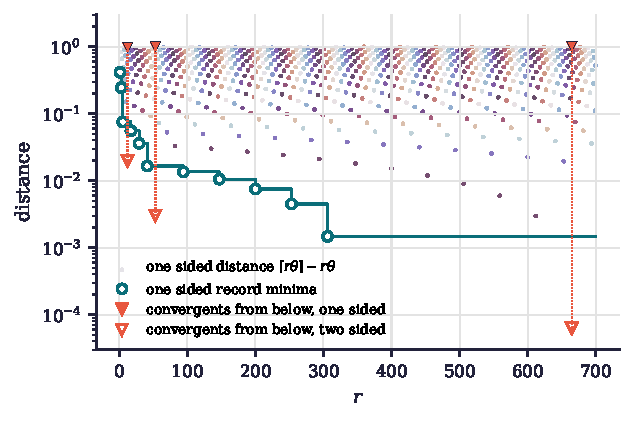
\includegraphics[width=\textwidth]{figures/ch8_onesided.pdf}
\caption{The one sided distance $\delta(r)=\lceil r\theta\rceil-r\theta$ for
$r\leq700$. Circles mark the record minima, which are the rungs
$1,3,5,17,29,41,94,147,200,253,306$. Triangles mark the convergents from below,
$q_4=12$, $q_6=53$ and $q_8=665$: filled at their one sided distance, which is
close to $1$, and open at their two sided distance $\|q\theta\|$, which is
small.}
\label{fig:ch8:onesided}
\end{figure}

\begin{figure}[ht]
\centering
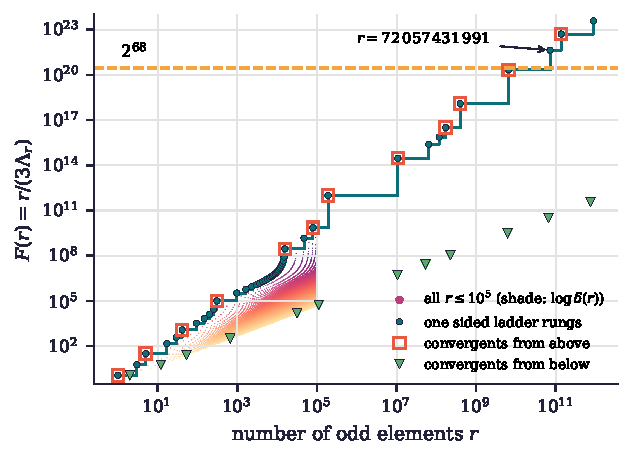
\includegraphics[width=\textwidth]{figures/ch8_records.pdf}
\caption{The bound $F(r)=r/(3\Lambda_r)$ on the least element of a cycle with $r$ odd elements. Shaded by $\log\delta(r)$: all $r\leq10^5$. Staircase: the rungs of the one sided ladder up to $10^{12}$, joined as a running maximum. Squares and triangles: convergent denominators from above and below. The dashed line is the verified range $2^{68}$; the first rung above it is $r=72\,057\,431\,991$.}
\label{fig:ch8:records}
\end{figure}

\section{The mediant lemma}\label{sec:ch8:mediant}

We now show that the rungs are not merely where the records happen to lie in
a finite search, but where they must lie. The argument is a single
observation about the additivity of $\delta$.

\begin{lemma}[Mediant lemma]\label{lem:ch8:mediant}
Let $1\leq r'<r$ with $\delta(r')<\delta(r)$, and put $d=r-r'$. Then
\begin{equation}\label{eq:ch8:additive}
  \delta(r)=\delta(r')+\delta(d).
\end{equation}
Consequently $\delta(r)/r$ is the mediant of $\delta(r')/r'$ and
$\delta(d)/d$, and
\begin{equation}\label{eq:ch8:mediantineq}
  \frac{\delta(r)}{r}\geq\min\Bigl(\frac{\delta(r')}{r'},\
  \frac{\delta(d)}{d}\Bigr).
\end{equation}
\end{lemma}

\begin{proof}
For every $x\geq1$, $\delta(x)=\lceil x\theta\rceil-x\theta$ is congruent to
$-x\theta$ modulo $1$ and lies in $(0,1)$; since $x\theta\notin\Z$, it is
the unique number in $[0,1)$ with that property. The number
$\delta(r)-\delta(r')$ is congruent to $-(r-r')\theta=-d\theta$ modulo $1$, and
by hypothesis it lies in $(0,1)$, because both terms lie in $(0,1)$ and the
first is larger. By uniqueness it equals $\delta(d)$. For the inequality,
$\delta(r)/r=(\delta(r')+\delta(d))/(r'+d)$ is a weighted average of
$\delta(r')/r'$ and $\delta(d)/d$, with weights $r'/r$ and $d/r$, and is
therefore at least the smaller of the two.
\end{proof}

The content of \eqref{eq:ch8:additive} is that there is no wrap around: the
congruence $\delta(r)\equiv\delta(r')+\delta(d)$ modulo $1$ always holds, and
the hypothesis $\delta(r')<\delta(r)$ upgrades it to an equality. We now draw
two consequences.

\begin{corollary}\label{cor:ch8:firstfeasible}
Let $\varepsilon>0$ and suppose some $r\geq1$ satisfies
$\delta(r)<r\varepsilon$. Then the smallest such $r$ is a $\delta$ record.
\end{corollary}

\begin{proof}
Let $r_*$ be the smallest $r$ with $\delta(r)<r\varepsilon$, and suppose it is
not a $\delta$ record. Then there is $r'<r_*$ with $\delta(r')\leq\delta(r_*)$.
Equality is impossible, since it would make $(r_*-r')\theta$ an integer; so
$\delta(r')<\delta(r_*)$. Put $d=r_*-r'$, so $1\leq d<r_*$. By minimality of
$r_*$, both $\delta(r')\geq r'\varepsilon$ and $\delta(d)\geq d\varepsilon$.
By \eqref{eq:ch8:mediantineq}, $\delta(r_*)/r_*\geq\varepsilon$, a
contradiction.
\end{proof}

\begin{corollary}\label{cor:ch8:recordsrecords}
If $r$ is a strict record of $r\mapsto r/\delta(r)$, meaning
$r/\delta(r)>r'/\delta(r')$ for every $1\leq r'<r$, then $r$ is a $\delta$
record.
\end{corollary}

\begin{proof}
If not, there is $r'<r$ with $\delta(r')<\delta(r)$ (equality being impossible
as before). With $d=r-r'<r$, \eqref{eq:ch8:mediantineq} gives
$r/\delta(r)\leq\max(r'/\delta(r'),d/\delta(d))$, contradicting strictness.
\end{proof}

Since $F(r)=r/(3\delta(r)\log2)$ is a constant multiple of $r/\delta(r)$,
\cref{cor:ch8:recordsrecords} combined with \cref{thm:ch8:onesided} locates
the records of $F$ exactly.

\begin{proposition}[Where the records are]\label{prop:records}
Every $r$ at which $r\mapsto F(r)=r/(3\Lambda_r)$ attains a strict record is a
rung of the semiconvergent\index{convergent}\index{semiconvergent} ladder approximating $\theta$ from above, that is,
$r=q_{k-1}+jq_k$ with $k\geq0$ even and $1\leq j\leq a_{k+1}$. Moreover, for
every verified range\index{verification range} $X$, the smallest $r$ that is not excluded in the sense
of \cref{def:ch8:excl} is such a rung.
\end{proposition}

\begin{proof}
The first statement is \cref{cor:ch8:recordsrecords} combined with
\cref{thm:ch8:onesided}. The second is \cref{cor:ch8:firstfeasible} with
$\varepsilon=1/(3X\log2)$, followed by \cref{thm:ch8:onesided}. (Such an $r$
exists: by \cref{lem:ch8:basic}(iv), at the convergents from above
$\delta(q_k)=p_k-q_k\theta<1/q_{k+1}$, which is eventually below
$q_k\varepsilon$.)
\end{proof}

The converse holds as well, so the strict records of $F$ are exactly the rungs, as the classical theorem~\cite[Theorem~4.5(ii)]{hancl2019} also says. Along the rungs $r$ increases while $\delta$ decreases, by \cref{thm:ch8:onesided}, so $F$ increases; and for any $r'$ the first point at which $F$ attains its maximum over $[1,r']$ is a strict record, hence a rung $u'\leq r'$, so every rung $u>r'$ has $F(u)>F(u')\geq F(r')$.
For $\lt$ every rung
up to $72\,057\,431\,991$ is accordingly a record of $F$ (the values in
\cref{tab:ch8:ladder} increase), and the exact scan to $3\times10^6$ found
the records of $F$ and the $\delta$ records to coincide there. The cycle bound
below does not need the converse.

\begin{remark}[Ties, and a warning about arithmetic]\label{rem:ch8:ties}
Multiples of a rung produce exact ties. If $t\,\delta(q)<1$ for an integer $t\geq2$ then
$\delta(tq)=t\,\delta(q)$, since $tq\theta=t\lceil q\theta\rceil-t\delta(q)$,
so $F(tq)=F(q)$ and the multiple ties with its generator rather than beating
it; by \cref{cor:ch8:recordsrecords} it cannot be a strict record.
Halbeisen\index{Halbeisen, L.} and Hungerb\"uhler\index{Hungerbuhler, N.@Hungerb\"uhler, N.}~\cite[\S4.4]{halbeisen1997} observe these ties for Eliahou's criterion, at multiples of a convergent denominator. In floating
point arithmetic such ties break at random. With $\Lambda_r$ evaluated in
double precision as $s\log2-r\log3$, $s=\lfloor r\theta\rfloor+1$, a scan of
$r\leq10^6$ reports $918=3\cdot306$, $46\,803=3\cdot15\,601$ and
$952\,685=5\cdot190\,537$ as new records (script \texttt{ch08\_ties.py});
evaluated instead as $(\lceil r\theta\rceil-r\theta)\log2$, the same scan
happens to report no spurious records, the ties breaking the other way or not
at all.
At $150$ digits the differences $\delta(tq)-t\delta(q)$ for $46\,803$, $571\,611=3\cdot190\,537$ and $952\,685$ come out as $-2.5\times10^{-147}$, $0$ and $0$, but the spurious records do not disappear: a tie is an exact equality between irrational numbers, so rounding decides it at every precision, and the same scan at $150$ digits reports $15=3\cdot5$ and $571\,611$ as new records in the first form, and $46\,803$ and $571\,611$ in the second.
The cure is exact arithmetic: $F(r)>F(r')$ if and only if $r\lceil r'\theta\rceil>r'\lceil r\theta\rceil$, a comparison of integers once the ceilings are known, and a scan of $r\leq10^6$ in this form finds exactly the rungs as its strict records.
This is one more reason to prefer an argument that locates the records over
a search that merely finds them.
\end{remark}

\section{The cycle length bound}\label{sec:ch8:bound}

\Cref{prop:records} turns the search for the sharp bound into a short
computation over the rungs. For $\lt$ there are only $44$ rungs up to
$72\,057\,431\,991$, and \cref{tab:ch8:ladder} lists the last eleven of them
with the value of $F$ at each.

\begin{table}[ht]
\centering
\caption{The upper ladder rungs from $q_9$ to the first rung exceeding
$2^{68}$, with $s=\lceil r\theta\rceil$ and $F(r)=r/(3\Lambda_r)$, computed
at $150$ digits. The decomposition column writes each rung as a convergent denominator or as
$q_{k-1}+jq_k$.}
\label{tab:ch8:ladder}
\small
\begin{tabular}{@{}rrrl@{}}
\toprule
$r$ & $s$ & $F(r)$ & rung \\
\midrule
$15\,601$ & $24\,727$ & $2.86\times10^{8}$ & $q_9$ \\
$47\,468$ & $75\,235$ & $1.45\times10^{9}$ & $q_9+q_{10}$ \\
$79\,335$ & $125\,743$ & $7.22\times10^{9}$ & $q_{11}$ \\
$190\,537$ & $301\,994$ & $9.85\times10^{11}$ & $q_{13}=q_{11}+q_{12}$ \\
$10\,781\,274$ & $17\,087\,915$ & $2.94\times10^{14}$ & $q_{15}=q_{13}+q_{14}$ \\
$64\,497\,107$ & $102\,225\,496$ & $2.46\times10^{15}$ & $q_{15}+q_{16}$ \\
$118\,212\,940$ & $187\,363\,077$ & $7.49\times10^{15}$ & $q_{15}+2q_{16}$ \\
$171\,928\,773$ & $272\,500\,658$ & $3.20\times10^{16}$ & $q_{17}$ \\
$397\,573\,379$ & $630\,138\,897$ & $1.25\times10^{18}$ & $q_{19}=q_{17}+q_{18}$ \\
$6\,586\,818\,670$ & $10\,439\,860\,591$ & $2.17\times10^{20}$ & $q_{21}=q_{19}+q_{20}$ \\
$72\,057\,431\,991$ & $114\,208\,327\,604$ & $4.36\times10^{21}$ & $q_{21}+q_{22}$ \\
\bottomrule
\end{tabular}
\end{table}

\begin{theorem}[Cycle length bound]\label{thm:cycles}
Let $X$ be a verified range\index{verification range} in the sense of \cref{def:ch8:excl}.
\begin{enumerate}[label=(\roman*),leftmargin=2em]
\item \emph{Block form.} If $B_j\leq X$ for $j=0,1,\dots,K$, then every
  nontrivial cycle has $r\geq q_{K+1}$ odd elements.
\item \emph{Sharp form.} Every nontrivial cycle has $r\geq r_*(X)$ odd
  elements, where $r_*(X)$ is the smallest rung $u$ of the upper ladder with
  $F(u)>X$.
\end{enumerate}
With $X=2^{68}$, verified by Ba\v{r}ina\index{Barina, D.@Ba\v{r}ina, D.}~\cite{barina2021}, part (i) gives
\[
  r\geq q_{21}=6\,586\,818\,670,
\]
and part (ii) gives
\[
  r\geq72\,057\,431\,991,\qquad s\geq114\,208\,327\,604 .
\]
Thus a nontrivial cycle has at least $7.2\times10^{10}$ steps of $S$, at least
$1.14\times10^{11}$ steps of $T$, and at least $1.86\times10^{11}$ steps of
$T_0$.
\end{theorem}

\begin{proof}
By \cref{cor:ch8:excl} the number $r$ of odd elements of a nontrivial cycle is
not excluded, so $F(r)>X$.

(i) If $1\leq r<q_{K+1}$, then $q_j\leq r<q_{j+1}$ for some $0\leq j\leq K$
(recall $q_0=1$), and \cref{lem:block} gives $F(r)<B_j\leq X$, so $r$ is
excluded. With $X=2^{68}$, \cref{tab:cycles} and the values for $k\leq7$ in
its caption show $B_j\leq B_{20}=2.29\times10^{19}<2^{68}$ for all $j\leq20$,
so $K=20$ is admissible and $r\geq q_{21}$.

(ii) By \cref{prop:records}, the smallest nonexcluded $r$ is an upper ladder
rung $u$, and by definition of exclusion it is the smallest rung with
$F(u)>X$. So every $r<r_*(X)$ is excluded. With $X=2^{68}$, the $44$ rungs up
to $72\,057\,431\,991$ were evaluated at $150$ digits (script
\texttt{ch08\_bounds.py}); all before the last have $F(u)\leq
2.1689\times10^{20}<2^{68}=2.9515\times10^{20}$, the maximum being attained at
$u=q_{21}$, while $F(72\,057\,431\,991)=4.3585\times10^{21}>2^{68}$. Hence
$r_*(2^{68})=72\,057\,431\,991$. For the number of halvings, $s>r\theta\geq
r_*\theta$ and $s$ is an integer, so $s\geq\lceil r_*\theta\rceil=
114\,208\,327\,604$. The step counts follow from
\cref{rem:ch8:bookkeeping}: $r$ steps of $S$, $s$ of $T$ and $r+s\geq
186\,265\,759\,595$ of $T_0$.
\end{proof}

The first part uses only the property of best
approximation, and the second part uses the one sided theorem and the mediant lemma\index{mediant lemma}, and the numerical
evaluation involves margins that are enormous compared with the precision
used: the closest call is the ratio $2^{68}/F(q_{21})=1.36$, and the values of
$\delta$ involved are of order $10^{-11}$, computed with errors below
$10^{-130}$. The factor of about eleven between the two parts measures what
the block bound gives away by covering a whole interval with a single worst
case.

With the verification range $2^{71}$ of Ba\v{r}ina\index{Barina, D.@Ba\v{r}ina, D.}~\cite{barina2025}, part (i) improves to $r\geq q_{22}=65\,470\,613\,321$, since $B_{21}=2.16\times10^{21}<2^{71}=2.36\times10^{21}$, while part (ii) is unchanged, since $F(72\,057\,431\,991)=4.36\times10^{21}>2^{71}$.

\subsection{Exact versus crude}

There is an intermediate argument, which uses the $\delta$ records but not
the mediant lemma\index{mediant lemma}, and it can be much weaker. Let
$q_1'<q_2'<\cdots$ be the $\delta$ records. If a cycle has $r$ odd elements
and $q_j'$ is the largest record not exceeding $r$, then
$\delta(r)\geq\delta(q_j')$ by the definition of a record, and
$\delta(r)<r\varepsilon$ by \cref{cor:ch8:excl}, so $r>\delta(q_j')/\varepsilon$
and $r\geq q_j'$. Minimizing over the unknown $j$,
\begin{equation}\label{eq:ch8:crude}
  r\geq\min_j\max\Bigl(q_j',\ \frac{\delta(q_j')}{\varepsilon}\Bigr).
\end{equation}
The same bound appears in our unpublished note on AlphaProof
Nexus~\cite{polsonsokolov2026nexus}. It is valid, but loose. The reason is that
it uses the single value $\delta(q_j')$ as a lower bound for $\delta$ on the
whole block $[q_j',q_{j+1}')$, so it cannot exclude any $r$ in that block
beyond $\delta(q_j')/\varepsilon$, even though $\delta(r)$ there is in fact
much larger. The mediant lemma shows that nothing inside a block needs to be
checked at all: only the rungs matter, and at each rung one compares the exact
$\delta$ with $r\varepsilon$. \Cref{tab:ch8:crude} compares the two for
several verification ranges\index{verification range} (script \texttt{ch08\_crude.py}, at $80$ digits).

\begin{table}[ht]
\centering
\caption{Lower bounds on the number $r$ of odd elements of a nontrivial cycle,
for several verification ranges $X$: the exact first nonexcluded $r$ of
\cref{thm:cycles}(ii), with the corresponding $s=\lceil r\theta\rceil$, and
the crude bound \eqref{eq:ch8:crude}. The ranges up to $2^{71}$ are
verified~\cite{barina2021,barina2025}; the row $2^{72}$ shows what the method would give.}
\label{tab:ch8:crude}
\small
\begin{tabular}{@{}lrrr@{}}
\toprule
$X$ & exact $r_*(X)$ & $s$ & crude bound \\
\midrule
$2^{40}$ & $10\,781\,274$ & $17\,087\,915$ & $212\,781$ \\
$2^{60}$ & $397\,573\,379$ & $630\,138\,897$ & $397\,573\,379$ \\
$2^{68}$ & $72\,057\,431\,991$ & $114\,208\,327\,604$ & $8\,963\,457\,697$ \\
$2^{71}$ & $72\,057\,431\,991$ & $114\,208\,327\,604$ & $71\,707\,661\,575$ \\
$2^{72}$ & $137\,528\,045\,312$ & $217\,976\,794\,617$ & $78\,073\,328\,038$ \\
\bottomrule
\end{tabular}
\end{table}

At $2^{40}$ the crude bound is fifty times weaker: it is determined by the
record $q_{13}=190\,537$, with $\delta(q_{13})/\varepsilon=212\,780.2$, whereas
the next rung that is actually feasible is $q_{15}=10\,781\,274$. At $2^{68}$
the crude bound is determined by $q_{21}$, with
$\delta(q_{21})/\varepsilon=8\,963\,457\,696.8$, and it is eight times weaker
than the exact value. At $2^{60}$ the two coincide: the record $q_{19}=397\,573\,379$ is
itself feasible, and the preceding record $q_{17}$ has
$\delta(q_{17})/\varepsilon\approx6.2\times10^{9}$, which already exceeds
$q_{19}$, so the minimum in \eqref{eq:ch8:crude} is attained at $q_{19}$
with value $q_{19}$.

The table also shows how slowly the exact bound responds to verification.
Moving from $2^{68}$ to $2^{71}$, the step taken by Ba\v{r}ina\index{Barina, D.@Ba\v{r}ina, D.}~\cite{barina2025}, gives the exact bound no improvement whatever, because the
rung $r=72\,057\,431\,991$ has $F(r)=4.3585\times10^{21}=2^{71.884}$: any
verified range below about $2^{71.9}$ leaves that rung feasible. For the sharp form of \cref{thm:cycles}, a
verification past that point, for instance to $2^{72}$, would move the bound
to the next rung, $r\geq137\,528\,045\,312=q_{23}$, and further progress would
require passing $F(q_{23})=5.10\times10^{22}$. The bound $r\geq137\,528\,045\,312$ itself already holds unconditionally: it is the current record, which follows from Hercher's sharper accounting of the cycle together with the verification to $2^{71}$ (\cref{rem:attribution}).
The return on computation is
stepwise, in a way dictated entirely by the
continued fraction\index{continued fraction}; over many steps the bound grows roughly like the
square root of the verified range, from $1.08\times10^{7}$ at $2^{40}$ to
$7.2\times10^{10}$ at $2^{68}$.


\subsection{Verification thresholds}\label{sec:ch8:thresholds}

Since $r_*(X)$ is a step function of the verification range\index{verification range}, it is natural to
ask exactly where the steps are. The first rung $u$ not excluded at $X$ changes
precisely when $\log_2X$ crosses $\log_2F(u)$ for the current rung $u$, so the
thresholds are the values $\log_2F(u)$ along the sequence of successive
$r_*$. \Cref{tab:ch8:thresholds} lists them for $60\le\log_2X\le90$ and
\cref{fig:ch8:thresholds} draws the staircase (script
\texttt{ch08\_profile.py}, at $700$ digits).

\begin{table}[ht]
\centering\small
\caption{The sharp bound $r_*(X)$ as a function of the verification range.
Each row gives the rung $r_*$, the corresponding $s=\lceil r_*\theta\rceil$
and the interval of $\log_2X$ on which it is the bound.}
\label{tab:ch8:thresholds}
\begin{tabular}{@{}rrc@{}}
\toprule
$r_*$ & $s$ & range of $\log_2X$ \\
\midrule
$397\,573\,379$ & $630\,138\,897$ & $[54.830,\ 60.119)$ \\
$6\,586\,818\,670$ & $10\,439\,860\,591$ & $[60.119,\ 67.556)$ \\
$72\,057\,431\,991$ & $114\,208\,327\,604$ & $[67.556,\ 71.884)$ \\
$137\,528\,045\,312$ & $217\,976\,794\,617$ & $[71.884,\ 75.433)$ \\
$890\,638\,885\,193$ & $1\,411\,629\,234\,715$ & $[75.433,\ 78.333)$ \\
$1\,643\,749\,725\,074$ & $2\,605\,281\,674\,813$ & $[78.333,\ 79.456)$ \\
$2\,396\,860\,564\,955$ & $3\,798\,934\,114\,911$ & $[79.456,\ 80.287)$ \\
$5\,409\,303\,924\,479$ & $8\,573\,543\,875\,303$ & $[82.796,\ 84.500)$ \\
$11\,571\,718\,688\,839$ & $18\,340\,740\,190\,704$ & $[84.500,\ 87.951)$ \\
$64\,021\,008\,208\,555$ & $101\,470\,897\,268\,921$ & $[87.951,\ 90.590)$ \\
\bottomrule
\end{tabular}
\end{table}

Three features stand out. The range $2^{68}$ of \cref{thm:cycles} sits just above a
threshold, at $67.556$, which is why it yields the rung $72\,057\,431\,991$
rather than $6\,586\,818\,670$. The current range $2^{71}$~\cite{barina2025} lies in the same step, and so does the range $1536\cdot2^{60}=2^{70.585}$ at which Hercher\index{Hercher, C.}~\cite[Corollary~29]{hercher2023} obtains $r\geq1.375\times10^{11}$, now the record;
so the difference between our bound and that
record comes entirely from his sharper accounting of the
cycle, not from a larger range. And the steps between $2^{78}$ and $2^{83}$
are close together, because the partial quotient $a_{25}=7$ produces a ladder of seven nearby rungs $q_{23}+jq_{24}=137\,528\,045\,312+j\cdot753\,110\,839\,881$, $1\leq j\leq7$, of which the table shows the
first three and the last; the intermediate rungs occupy $[80.287,\ 82.796)$.

\begin{figure}[ht]
\centering
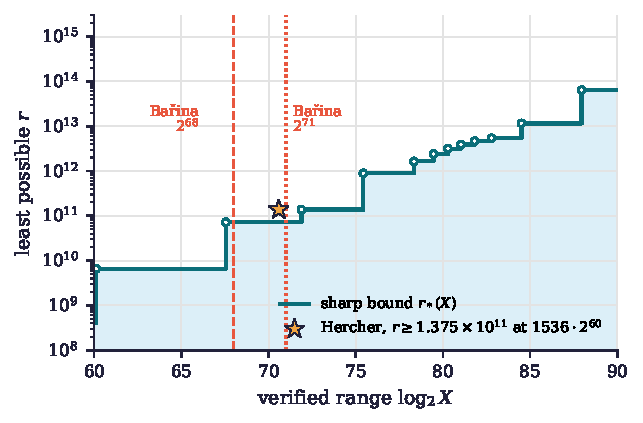
\includegraphics[width=\textwidth]{figures/ch8_thresholds.pdf}
\caption{The sharp bound $r_*(X)$ against the verification range $\log_2X$.
Every step is a rung of the one sided ladder of $\lt$. The dashed line marks
the range $2^{68}$ of Ba\v{r}ina~\cite{barina2021} and the dotted line his current range $2^{71}$~\cite{barina2025}, which lies in the same step. The star is the bound $r\geq1.375\times10^{11}$ that Hercher's sharper accounting of the cycle gives at
$1536\cdot2^{60}$; conditional when it was published, it is the current record since the verification to $2^{71}$.}
\label{fig:ch8:thresholds}
\end{figure}

\subsection{The literature}

\begin{remark}[Attribution]\label{rem:attribution}
The method of this section is not new, and we claim no priority for any
numerical bound. It goes back to Crandall\index{Crandall, R. E.}~\cite{crandall1978}, whose criterion is in substance the block bound of \cref{lem:block}, and to Eliahou~\cite{eliahou1993}. Steiner\index{Steiner, R. P.}~\cite{steiner1977} showed in 1977 that there is no
nontrivial cycle consisting of a single ascending run followed by a single
descending run (a $1$ cycle), using the continued fraction\index{continued fraction} of $\lt$ together
with Baker\index{Baker, A.}'s theory\index{Baker method} of linear forms in logarithms. Eliahou\index{Eliahou, S.}~\cite{eliahou1993}
combined the continued fraction of $\theta$ with verification to $2^{40}$ and
showed in 1993 that a nontrivial cycle has at least $17\,087\,915$ elements
under $T$; our method reproduces this figure exactly, as the value of $s$ at
$r_*(2^{40})=10\,781\,274$ in \cref{tab:ch8:crude}, which we regard as a
check on the implementation. The figure $q_{21}=6\,586\,818\,670$ of \cref{thm:cycles}(i) is also in the literature: Lagarias\index{Lagarias, J. C.}'s overview~\cite[\S6.1, item~(W2)]{lagarias2010overview} reports it from Eliahou's criterion with the smaller verification range $20\cdot2^{58}\approx5.76\times10^{18}$ of item~(W1). The bound $r\geq72\,057\,431\,991$ of \cref{thm:cycles}(ii) coincides with the record $r>7.2\times10^{10}$ that Hercher\index{Hercher, C.}~\cite{hercher2023} credits to Hercher and Puchert\index{Puchert, S.}~\cite{hercher2018,puchert2018}; with the verification range $87\cdot2^{60}$, Hercher~\cite{hercher2018} had shown that a nontrivial cycle has at least $p_{21}+q_{21}=17\,026\,679\,261$ elements under $T_0$.
Simons\index{Simons, J.} and de Weger\index{de Weger, B.}~\cite{simons2005} extended
Steiner's approach to $m$ cycles, cycles with $m$ ascending runs, ruling them
out for $m\leq68$ by combining continued fractions and lattice reduction with an explicit lower bound for $s\log2-r\log3$ derived from Rhin\index{Rhin, G.}'s Pad\'e approximation measure~\cite{rhin1987}, and
Hercher\index{Hercher, C.}~\cite[Theorem~23]{hercher2023} carried this to $m\leq91$. Hercher~\cite[Corollary~29]{hercher2023} also showed, by a sharper accounting of the
cycle structure than the crude inequality $\log(1+1/(3x_i))\leq1/(3M)$ used
in \cref{lem:cycleid}, that verification\index{verification range} up to $3\cdot2^{69}=1536\cdot2^{60}$ would give $r\geq1.375\times10^{11}$; with the crude inequality one needs $3781\cdot2^{60}$, the value $4.36\times10^{21}$ of $F$ at $r=72\,057\,431\,991$~\cite[Remark~28]{hercher2023}. Ba\v{r}ina\index{Barina, D.@Ba\v{r}ina, D.}~\cite{barina2025} has since verified the conjecture up to $2^{71}>3\cdot2^{69}$, so this bound now holds unconditionally and is the current record: every nontrivial cycle has $r\geq137\,528\,045\,312=q_{23}$ odd elements, and at least $p_{23}+q_{23}=355\,504\,839\,929$ elements under $T_0$, as Ba\v{r}ina notes~\cite[\S6]{barina2025}.
The record structure itself is classical: the first
nonexcluded $r$ is the least denominator of a fraction $s/r$ in the interval
$(\theta,\theta+\varepsilon)$, and the least denominator fraction in an interval
is read off the continued fraction expansion, a lemma Hercher states and uses
(his Lemma 22) and which underlies Eliahou's computation; in the form of \cref{thm:ch8:onesided} and \cref{prop:records} it is the description of the best one sided approximations stated and proved in~\cite[Theorem~4.5(ii)]{hancl2019}. The mediant lemma\index{mediant lemma}
(\cref{lem:ch8:mediant}) reduces the question to the $\delta$ records in two lines, and \cref{thm:ch8:onesided} identifies those with the rungs;
together they keep the certificate\index{certificate} of \cref{sec:ch8:certificate} short. Halbeisen\index{Halbeisen, L.} and Hungerb\"uhler\index{Hungerbuhler, N.@Hungerb\"uhler, N.}~\cite{halbeisen1997} go further in another direction: they replace the crude inequality by the optimal criterion, which is attained by the balanced parity word, and they observe both the harmlessness of the convergents from the wrong side (\cref{rem:ch8:false}) and the exact ties at multiples (\cref{rem:ch8:ties}). What we add
is that certificate and the analysis of \cref{sec:ch8:limits}, which shows exactly what Diophantine\index{Diophantine approximation}
information cannot do (a point that Halbeisen and Hungerb\"uhler~\cite[\S5]{halbeisen1997} make in another form: rational cycles satisfy the same inequalities, and their least elements grow with the length) and what arithmetic information would suffice.
\end{remark}

\begin{remark}[Comparison with Baker's method]\label{rem:ch8:baker}
Baker's theory gives lower bounds for linear forms in logarithms of algebraic
numbers, and for two logarithms the explicit estimates of Laurent\index{Laurent, M.}, Mignotte\index{Mignotte, M.}
and Nesterenko\index{Nesterenko, Yu.}~\cite[Corollary~2]{laurent1995} give, for the form
$\Lambda=s\log2-r\log3$, a bound of the shape $\log\Lambda\geq-C(\log r)^2$
with an explicit absolute constant $C$; precisely, $\log\Lambda\geq-24.34\,\log3\,\bigl(\max\{\log b'+0.14,\,21\}\bigr)^2$ with $b'=r+s/\log3\approx2.44\,r$.
For $r\leq4.6\times10^8$ the maximum is $21$ and the bound is $-24.34\cdot\log3\cdot441\approx-11\,792$, so it gives only $\Lambda\geq e^{-11800}$ there, and $\Lambda\geq e^{-11900}$ for $r\leq5\times10^8$: a bound on
$M$ that is astronomically larger than anything verification can reach,
whereas the actual values of $\Lambda_r$ near $r=10^5$, from
\cref{tab:ch8:conv}, are of order $10^{-6}$. The reason is structural. Baker's
theorem bounds $\Lambda$ uniformly in $r$, with no knowledge of which $r$ are
dangerous; here we enumerate the dangerous $r$, so the exact value of
$\Lambda_r$ is available. Transcendence methods become indispensable only
when a bound valid for all $r$ simultaneously is wanted, as for the $m$ cycle
results of Steiner, Simons and de Weger, and Hercher, where $r$ is unbounded.
\end{remark}

\section{What Diophantine approximation cannot do}\label{sec:ch8:limits}

One might believe that the cycle half of the conjecture is, at bottom,
a question about how well $\lt$ can be approximated by rationals, and that a
sufficiently strong effective irrationality measure\index{irrationality measure} for $\lt$ would settle it.
This section shows that the belief is false, quantifies what such a measure
would give, and identifies the missing ingredient.

\begin{remark}[What an irrationality measure gives]\label{rem:irrmeasure}
Suppose $\nu$ is an effective irrationality measure for $\lt$ with constant
$c$, meaning that $|\lt-s/r|\geq c\,r^{-\nu}$ for all integers $s$ and
$r\geq1$. Then $\delta(r)=s-r\theta=r(s/r-\theta)\geq c\,r^{1-\nu}$ with
$s=\lceil r\theta\rceil$, and \eqref{eq:ch8:maxM} becomes
\begin{equation}\label{eq:ch8:irrbound}
  M<F(r)\leq\frac{r^{\nu}}{3c\log2}.
\end{equation}
Since $\nu\geq2$ for every irrational number (\cref{lem:ch8:basic}(iv)), the
right side grows at least like $r^2$. Combined with $M>X$, the bound excludes
precisely the $r$ with $r^{\nu}<3cX\log2$, a finite range, and nothing beyond
it. In particular no irrationality measure, however good, bounds $M$ uniformly in $r$.
\end{remark}

The finite range is not a weakness of irrationality measures in particular.
It is forced by the structure of the problem.

\begin{proposition}[Diophantine insufficiency]\label{prop:ch8:insufficient}
For every $X\geq1$ there are infinitely many $r\geq1$ with
\[
  0<\delta(r)<\frac{r}{3X\log2},
\]
that is, infinitely many $r$ that are not excluded at verification range\index{verification range} $X$.
\end{proposition}

\begin{proof}
By \cref{thm:ch8:onesided} the one sided records $u_1<u_2<\cdots$ form an
infinite sequence along which $\delta(u_i)$ decreases strictly. Moreover
$\delta(u_i)\to0$: the convergents\index{convergent} $p_k/q_k$ with $k$ odd lie above $\theta$,
so $\lceil q_k\theta\rceil=p_k$ and $\delta(q_k)=p_k-q_k\theta<1/q_{k+1}$ by
\cref{lem:ch8:basic}(iv), and these $q_k$ are among the records. Put
$\varepsilon=1/(3X\log2)$. Once $\delta(u_i)<\varepsilon$, which holds for all
large $i$, we have $\delta(u_i)<\varepsilon\le u_i\varepsilon$, so $u_i$ is
not excluded.
\end{proof}

In words: the inequality \eqref{eq:ch8:maxM}, a verified range and any information about the number $\lt$ alone cannot together exclude all nontrivial cycles.

How large is the gap in practice? The best conceivable constant for $\nu=2$
consistent with the rungs computed so far is $c_2=\min_u u\,\delta(u)
=0.01773$, attained at $u=190\,537$ (the rung before the partial quotient
$55$), and the corresponding exclusion is $r<(3c_2X\log2)^{1/2}$.
\Cref{tab:ch8:insufficient} compares this with the exact $r_*(X)$. Even this
idealized measure, far better than any effective measure known (the explicit bound of Rhin~\cite{rhin1987}, in the form used by Simons and de Weger~\cite[Lemma~12]{simons2005}, corresponds to $\nu\approx14.3$), is beaten by
the ladder computation by factors from about two to more than fifty, because the ladder
uses the exact value of $\delta$ at each dangerous $r$ while the measure uses
a worst case. With exponents $\nu\geq3$ the best conceivable constant is
$c_\nu=\log_2(4/3)=0.4150$, attained at $r=1$, and at $X=2^{68}$ it excludes
only $r<6.3\times10^6$ for $\nu=3$ and $r<1.3\times10^5$ for $\nu=4$.

\begin{table}[ht]
\centering\small
\caption{Exclusion by an idealized measure with $\nu=2$ and $c_2=0.01773$
versus the exact ladder bound.}
\label{tab:ch8:insufficient}
\begin{tabular}{@{}lrrr@{}}
\toprule
$X$ & measure excludes $r<$ & exact $r_*(X)$ & ratio \\
\midrule
$2^{40}$ & $2.01\times10^{5}$ & $1.08\times10^{7}$ & $53.5$ \\
$2^{60}$ & $2.06\times10^{8}$ & $3.98\times10^{8}$ & $1.93$ \\
$2^{68}$ & $3.30\times10^{9}$ & $7.21\times10^{10}$ & $21.8$ \\
$2^{72}$ & $1.32\times10^{10}$ & $1.38\times10^{11}$ & $10.4$ \\
$2^{80}$ & $2.11\times10^{11}$ & $2.40\times10^{12}$ & $11.4$ \\
\bottomrule
\end{tabular}
\end{table}

\Cref{fig:ch8:irrprofile} shows the empirical irrationality profile of $\lt$:
for each convergent the exponent $\nu_k=-\log|\theta-p_k/q_k|/\log q_k$,
together with the next partial quotient. The exponents settle near $2$ (their
mean over $50\le k\le198$ is $2.010$), with excursions exactly where a large
partial quotient follows; the largest partial quotients among the first $199$
are $55$ (twice), $49$, $37$ and $33$. This is what one sees for a typical real
number, and it says nothing provable about $\lt$. In particular the profile
gives no evidence either way on whether the partial quotients of $\lt$ are
bounded; and by \cref{prop:ch8:insufficient}, even bounded partial quotients
would not finish the cycle half.

\begin{figure}[ht]
\centering
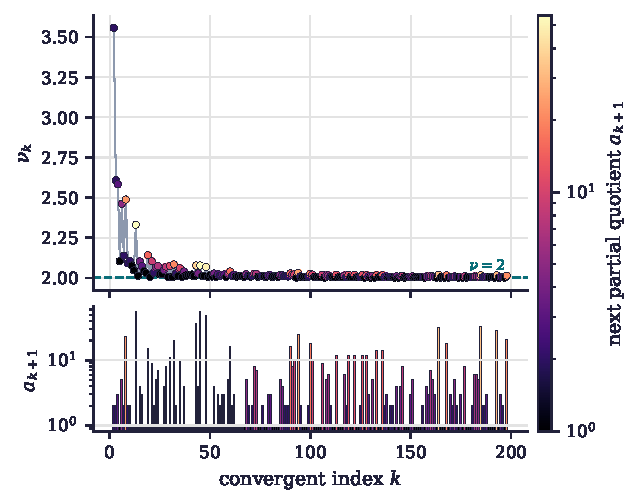
\includegraphics[width=\textwidth]{figures/ch8_irrprofile.pdf}
\caption{Empirical irrationality profile of $\lt$. Top: the exponent $\nu_k$
of the $k$th convergent, coloured by the next partial quotient. Bottom: the
partial quotients $a_{k+1}$ on a logarithmic scale. Large partial quotients
produce the visible excursions above $\nu=2$.}
\label{fig:ch8:irrprofile}
\end{figure}

\subsection{The window lemma}

What, then, is missing? The inequality \eqref{eq:ch8:maxM} is an
\emph{upper} bound on the least element of a cycle. The affine identity of
\cref{chap:parity} gives a matching \emph{lower} bound, and the two together
confine the least element to a window whose width is the real measure of our
ignorance.
In the rest of this section we write $m=r$ for the number of odd steps and $k=s$ for the number of steps of $T$, as in \cref{chap:parity}, so that $k$ is no longer a continued fraction index.

\begin{lemma}[Window lemma]\label{lem:ch8:window}
Let $x_1,\dots,x_r$ be the odd elements of a cycle of the accelerated map\index{accelerated map} $T$
with $r=m$ odd steps and $k=s$ steps in all, and put
$\Lambda=k\log2-m\log3>0$. Then every element $x$ of the cycle (odd or even)
satisfies
\begin{equation}\label{eq:ch8:window}
  \frac{3^m-2^m}{2^k-3^m}\;\le\;x,
  \qquad\text{and}\qquad
  M=\min_i x_i\;<\;\frac{m}{3\Lambda}\;\le\;F(m),
\end{equation}
where $(3^m-2^m)/(2^k-3^m)=(1-(2/3)^m)/(e^{\Lambda}-1)$, and $m/(3\Lambda)=F(m)$ exactly when $k=\lceil m\theta\rceil$. In particular the least
element lies in the window
$\bigl[(1-(2/3)^m)/(e^{\Lambda}-1),\ m/(3\Lambda)\bigr)$, whose endpoints have
ratio $\frac m3\cdot\frac{e^\Lambda-1}{\Lambda}(1-(2/3)^m)^{-1}$, which is
$\frac m3(1+o(1))$ as $\Lambda\to0$ and $m\to\infty$.
\end{lemma}

\begin{proof}
Let $x$ be any element of the cycle. Applying \eqref{eq:ch2:affine} to the
$k$ steps that return $x$ to itself gives $2^kx=3^mx+c_k(x)$, so
$x=c_k(x)/(2^k-3^m)$, the denominator being positive because $\Lambda>0$. By
the recursion \eqref{eq:ch2:crec}, an odd step at time $i$ contributes $2^i$,
multiplied by $3$ once for each later odd step, so
$c_k(x)=\sum_{j=0}^{m-1}3^{m-1-j}2^{i_j}$, where $0\le i_0<i_1<\cdots<i_{m-1}\le
k-1$ are the times of the odd steps. Since $i_j\ge j$, every term is at least
the corresponding term with $i_j=j$, hence
$c_k(x)\ge\sum_{j=0}^{m-1}3^{m-1-j}2^{j}=3^m-2^m$. This gives the lower bound,
and dividing numerator and denominator by $3^m$ gives the second form.
For the upper bound, the proof of \cref{lem:cycleid} with $r=m$ gives $\Lambda<\sum_i1/(3x_i)\le m/(3M)$, since $\log(1+u)<u$; and $\Lambda\ge\Lambda_m=\delta(m)\log2$ by \eqref{eq:ch8:Lambdar}, with equality exactly when $k=\lceil m\theta\rceil$, so $m/(3\Lambda)\le F(m)$.
The ratio of the endpoints is the quotient of the two
expressions, and $(e^\Lambda-1)/\Lambda\to1$, $(2/3)^m\to0$.
\end{proof}

For the trivial cycle, $m=1$ and $k=2$, the window is $[1,\ 1.159)$ and the
cycle sits at its left end. For the hypothetical cycles at the ladder rungs the
window is enormous: at the rung $r_*=72\,057\,431\,991$, with $k$ the
corresponding $s$, the lower end is $1.8\times10^{11}\approx2^{37.4}$ and the
upper end $4.4\times10^{21}=2^{71.9}$, a factor $r/3$ apart as the lemma
predicts (\cref{fig:ch8:window}). The verified range\index{verification range} $2^{68}$ removes the lower
part of the window, and what is left is exactly the gap that the sharp bound
of \cref{thm:cycles} measures.

\begin{corollary}[What arithmetic would suffice]\label{cor:ch8:window}
Suppose that for some function $f$ every nontrivial cycle with $m$ odd steps and $k$ steps in all satisfied the sharpened upper bound $M<m/(3\Lambda f(m))$, where $\Lambda=k\log2-m\log3$ is the value at that cycle.
\begin{enumerate}[label=(\roman*),leftmargin=2em]
\item If $f(m)\ge\frac m3\cdot\frac{e^{\Lambda}-1}{\Lambda}\bigl(1-(2/3)^m\bigr)^{-1}$ for every pair $(m,k)$ with $m\theta<k<2m$, then there are no nontrivial cycles.
\item If $f(m)\ge\frac m3(1+\eta)$ for some $\eta>0$ and all $m\ge m_0$, where $(1+\eta)(1-(2/3)^{m_0})>1$, let $\Lambda_0>0$ solve $(e^{\Lambda_0}-1)/\Lambda_0=(1+\eta)(1-(2/3)^{m_0})$. Then every nontrivial cycle with $m\ge m_0$ odd steps has least element $M<C=1/((1+\eta)\Lambda_0)$, which is about $1/(2\eta)$ when $\eta$ is small and $m_0$ large; so a verified range\index{verification range} $X\ge\max\bigl(C,\max_{m<m_0}F(m)\bigr)$ excludes all nontrivial cycles, with no further use of Diophantine\index{Diophantine approximation} approximation.
\end{enumerate}
\end{corollary}

\begin{proof}
A nontrivial cycle contains no element $1$, so every $x_i\ge3$ and \eqref{eq:ch8:prod} gives $2^k=\prod_i(3+1/x_i)<4^m$; with $\Lambda>0$ this is $m\theta<k<2m$.
(i) The hypothesis puts the upper end $m/(3\Lambda f(m))$ of the sharpened window at or below the lower end $(1-(2/3)^m)/(e^{\Lambda}-1)$ of \eqref{eq:ch8:window}, which is impossible.
(ii) The function $(e^{\Lambda}-1)/\Lambda$ increases from $1$ to $\infty$ on $(0,\infty)$.
For a cycle with $m\ge m_0$ and $\Lambda<\Lambda_0$ it is therefore below $(1+\eta)(1-(2/3)^{m_0})\le\frac{3f(m)}{m}(1-(2/3)^m)$, and the window is empty as in (i).
For a cycle with $m\ge m_0$ and $\Lambda\ge\Lambda_0$ the hypothesis gives $M<m/(3\Lambda_0f(m))\le1/((1+\eta)\Lambda_0)=C$.
For $m<m_0$, \cref{lem:ch8:window} gives $M<F(m)$.
So a nontrivial cycle would have $M<X$, whereas every element of a nontrivial cycle is at least $X$.
\end{proof}

The corollary converts the vague hope that ``the arithmetic of the parity word should help'' into a precise target: an improvement of the upper bound by a factor slightly more than $m/3$. A factor $\frac m3(1+\eta)$ for all large $m$ would confine the least element of every nontrivial cycle with many odd steps below about $1/(2\eta)$, and a finite verification would then exclude all nontrivial cycles.
Raising the lower end by such a factor, or splitting the factor between the two ends, empties the window only when $\Lambda$ is small; the cycles with $\Lambda$ bounded below would still need an upper bound on $M$ that does not grow with $m$.
By contrast, \cref{prop:ch8:insufficient}
shows that no improvement of the Diophantine side alone can work.

\begin{figure}[ht]
\centering
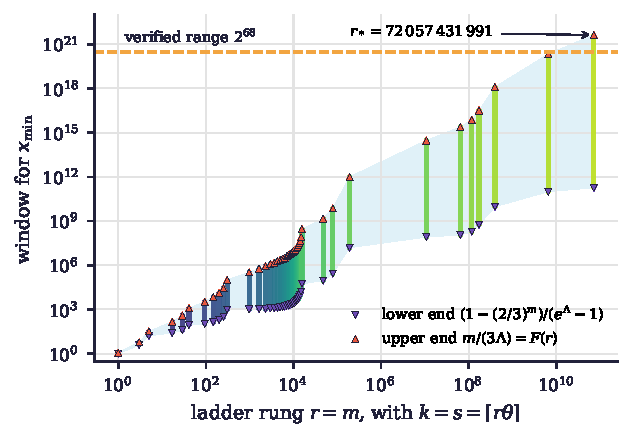
\includegraphics[width=\textwidth]{figures/ch8_window.pdf}
\caption{The window of \cref{lem:ch8:window} for the hypothetical cycles at
every rung of the one sided ladder up to $r_*(2^{68})$. Downward triangles are
the lower ends $(1-(2/3)^m)/(e^\Lambda-1)$, upward triangles the upper ends
$F(m)=m/(3\Lambda)$; the vertical segments are the windows. Only the rung
$r_*=72\,057\,431\,991$ reaches above the verified range $2^{68}$.}
\label{fig:ch8:window}
\end{figure}

\subsection{An exploration of parity words}

To see where actual cycles of rational numbers sit inside the window, we
enumerated all parity words with $m\le20$ ones and
$\lceil m\theta\rceil\le k\le2m$ letters (sampling $10^6$ words when there are
more than $3\times10^6$), computed $x=c_k(w)/(2^k-3^m)$ for each, and recorded
how close $c_k(w)$ comes to a multiple of $D=2^k-3^m$ (script
\texttt{ch08\_window.py}). Every word defines a cycle of $T$ on the rationals
with odd denominator, the rational cycles\index{rational cycles} of Lagarias\index{Lagarias, J. C.}~\cite{lagarias1990}, and
an integer cycle corresponds to $D\mid c_k(w)$. Three observations emerged.

First, the only integer hits for $m\le20$ are the words of the trivial cycle
$\{1,2\}$ repeated, at $k=2m$; this is of course consistent with
\cref{thm:cycles}.
The closest approaches of $c_k(w)/D$ to an integer are of the size predicted by a model in which the residues $c_k(w)\bmod D$ of the words examined are independent and uniform on the nonzero classes: over the $92$ shapes $(m,k)$ with at least $50$ words, the closest approach divided by its expected value under the model has mean $1.1$ and median $0.66$, where the model gives $1$ and about $\log2=0.69$, and the median drifts only from $0.87$ for $m\le12$ to $0.63$ for $m\ge13$ while the expected value itself falls from $8\times10^{-2}$ to $2\times10^{-7}$ (\cref{fig:ch8:words}, right).
We found no sign of a structural obstruction at
this scale, in either direction.

Second, the least element of a rational cycle can sit nearly anywhere in the window:
over all rotation classes with $m\le11$ the ratio of the least element to the
lower end of the window attains $1$ (the lower bound of
\cref{lem:ch8:window} is sharp, attained by the word with all odd steps
first), and the least element never exceeds $0.87$ of the upper end $m/(3\Lambda)$ of its window: the largest ratio, $3\log(4/3)=0.863$, is that of the trivial cycle repeated, and for $k<2m$ the ratio stays below $0.79$, while the harmonic mean of the odd elements, which is what the proof of \cref{lem:ch8:window} actually bounds, reaches $0.995$ of the upper end
(\cref{fig:ch8:words}, left).

Third, for the balanced words\index{balanced words}, the Christoffel words with $m$ ones spread as
evenly as possible among $k$ letters, which are the natural candidates for a
cycle with $k/m$ close to $\theta$, the least and greatest odd elements sit at nearly fixed fractions of the upper end when $k=\lceil m\theta\rceil$: for the $1154$ primitive balanced words ($\gcd(m,k)=1$) with $100\le m\le2000$, $x_{\min}/F(m)$ lies in $[0.719,\,0.724]$ and the greatest odd element in $[1.435,\,1.444]\,F(m)$, close to $1/(2\log2)=0.7213$ and $1/\log2=1.4427$.
(When $\gcd(m,k)>1$ the balanced word is a shorter one repeated and gives the same rational cycle; thus $m=400$ and $800$ repeat $m=200$.)
A heuristic explains the constants. For a balanced word the
odd elements of the cycle are nearly a geometric progression in $\log_2$, filling
an interval $[x_{\min},2x_{\min}]$ with $\log_2x$ nearly uniformly
distributed; then the mean of $1/x_i$ is about
$x_{\min}^{-1}\int_0^12^{-u}\,du=1/(2x_{\min}\log2)$, and
$\Lambda\approx\sum_i1/(3x_i)$ gives $F(m)=m/(3\Lambda)\approx2\log2\,x_{\min}$.
We record this as an observation, not a theorem: it says that for balanced
words the least element sits a fixed fraction below the top of the window, so
balanced words are as far as possible from the factor $m/3$ that
\cref{cor:ch8:window} asks for. Any arithmetic proof that there are no cycles
must therefore treat balanced words by divisibility, not by size.

\begin{figure}[ht]
\centering
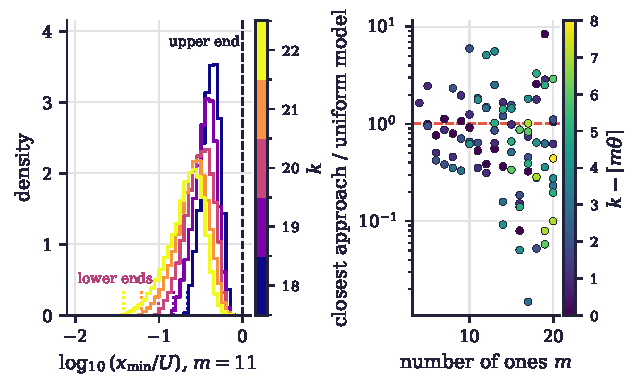
\includegraphics[width=\textwidth]{figures/ch8_words.pdf}
\caption{Left: distribution of $\log_{10}(x_{\min}/U)$, where $U=m/(3\Lambda)$ is the upper end of the window for the given $k$, over rotation classes
of rational cycles with $m=11$, for each $k$ from $\lceil m\theta\rceil=18$ to $2m=22$ (colour); the lower ends
of the windows are marked (dotted). Right: the closest approach of $c_k(w)/D$ to an
integer, relative to its expected value when the residues of the words examined are independent and uniform on the nonzero classes modulo $D$, for the shapes with at least $50$ words, against the number of ones $m$,
coloured by $k-\lceil m\theta\rceil$.}
\label{fig:ch8:words}
\end{figure}

\section{An exact certificate}\label{sec:ch8:certificate}

The bound of \cref{thm:cycles}(ii) was computed in floating point, at $150$ digits.
For a result of this kind it is worth having a certificate\index{certificate} that uses no
floating point at all: a list of integer inequalities that anyone can check,
and that a proof assistant could check. The mediant lemma\index{mediant lemma} and \cref{thm:ch8:onesided} make such a
certificate short, and we have built one (script \texttt{ch08\_certificate.py},
which runs in eleven seconds).

\paragraph{Step 1: an enclosure of $\lt$.} Take the convergents
\[
  \frac ab=\frac{1\,193\,652\,440\,098}{753\,110\,839\,881},\qquad
  \frac{a'}{b'}=\frac{217\,976\,794\,617}{137\,528\,045\,312},
\]
which lie on opposite sides of
$\theta$. The inequalities $2^a<3^b$ and $3^{b'}<2^{a'}$ certify
$a/b<\theta<a'/b'$, an interval of width exactly $1/(bb')=9.65\times10^{-24}$.
The powers are far too large to form, so each comparison is made by enclosing
$3^b$ between $L\cdot2^e$ and $U\cdot2^e$ with $320$ bit integer mantissas,
computed by repeated squaring with downward and upward truncation; every
truncation is itself an integer inequality, and $39$ squarings suffice.

\paragraph{Step 2: an enclosure of $\log2$.} The partial sums of
$\sum_{n\ge1}1/(n2^n)=\log2$ are lower bounds, and adding the tail bound
$1/((N+1)2^N)$ gives upper bounds; we use an enclosure of width
$9\times10^{-30}$. The exclusions in fact survive the crude replacement of
$\log2$ by $69/100$, and the final feasibility check survives $7/10$, which
follow from the sum to $n=7$: $1163/1680>69/100$ and
$1163/1680+1/1024<7/10$.

\paragraph{Step 3: the partial quotients.} The common prefix of the continued
fraction expansions of the two rational endpoints, less its last term, is
certified to be the beginning of the expansion of $\theta$:
\[ [1;1,1,2,2,3,1,5,2,23,2,2,1,1,55,1,4,3,1,1,15,1,9]. \]

\paragraph{Step 4: the rungs.} From these partial quotients the ladder rungs
are generated exactly, $44$ of them up to $72\,057\,431\,991$. For each rung
$u<r_*$ the exclusion $\delta(u)\ge u\varepsilon$ is checked as an inequality
between rationals built from the enclosures, never using more than $248$ bit
integers; the smallest certified margin is $\delta(u)/(u\varepsilon)>1.355$ (true value $1.361$), at
$u=6\,586\,818\,670$.
At $r_*$ itself the opposite inequality is certified from the upper end of the enclosure, $\delta(r_*)<7.97\times10^{-12}$, so that $\delta(r_*)/(r_*\varepsilon)<0.068$ (true value $0.0677$), and the bound is attained by the method.

\paragraph{Step 5: the records.} The enclosures of $\delta$ are certified to
decrease strictly along the rungs, as \cref{thm:ch8:onesided} predicts, a consistency check on the partial quotients; by that theorem the rungs are the records, and with the mediant lemma this certifies that no other $r$
needs checking. As an independent check, an exact integer scan of all
$r\le2\times10^6$ finds exactly the $37$ records predicted by the ladder.

\begin{table}[ht]
\centering\small
\caption{Selected rungs of the certificate at $X=2^{68}$: the rung $u$, its
numerator $s=\lceil u\theta\rceil$, a certified bound for $\delta(u)$ (a lower bound for $u<r_*$, an upper bound at $u=r_*$),
and the margin $\delta(u)/(u\varepsilon)$, which must exceed $1$ for
exclusion.}
\label{tab:ch8:certificate}
\begin{tabular}{@{}rrcr@{}}
\toprule
$u$ & $s$ & $\delta(u)$ & margin \\
\midrule
$15\,601$ & $24\,727$ & $>2.62\times10^{-5}$ & $>1.0\times10^{12}$ \\
$190\,537$ & $301\,994$ & $>9.30\times10^{-8}$ & $>2.99\times10^{8}$ \\
$10\,781\,274$ & $17\,087\,915$ & $>1.76\times10^{-8}$ & $>1.0\times10^{6}$ \\
$171\,928\,773$ & $272\,500\,658$ & $>2.58\times10^{-9}$ & $>9214$ \\
$397\,573\,379$ & $630\,138\,897$ & $>1.52\times10^{-10}$ & $>235.7$ \\
$6\,586\,818\,670$ & $10\,439\,860\,591$ & $>1.45\times10^{-11}$ & $>1.355$ \\
$72\,057\,431\,991$ & $114\,208\,327\,604$ & $<7.97\times10^{-12}$ & $<0.068$ \\
\bottomrule
\end{tabular}
\end{table}

The certificate is the bridge to a machine checked proof
(\cref{sec:ch8:lean}): every step is an inequality between integers of at
most a few hundred bits, plus two exponentiations handled by a verified
squaring routine.

\section{A sibling problem: Erd\H{o}s 125}\label{sec:ch8:erdos}

Good rational approximations\index{Diophantine approximation} to $\theta$, the raw material of the previous sections, appear in a different role
in a problem from the Erd\H{o}s collection that was settled in 2026.

\subsection{The problem}

Let $A$ be the set of nonnegative integers whose base $3$ digits all lie in
$\{0,1\}$, and $B$ the set of nonnegative integers whose base $4$ digits all
lie in $\{0,1\}$. Then $|A\cap[0,3^n-1]|=2^n$ and $|B\cap[0,4^n-1]|=2^n$, so
$|A\cap[0,N]|$ is of order $N^{\log2/\log3}=N^{0.631}$ and $|B\cap[0,N]|$ of
order $N^{1/2}$. The number of pairs $(a,b)$ with $a+b\leq N$ is therefore of
order $N^{1.131}$, which exceeds $N$ by a power, and positive density of the
sumset $A+B$ is the naive guess. Burr\index{Burr, S. A.}, Erd\H{o}s\index{Erdos, P.@Erd\H{o}s, P.}, Graham\index{Graham, R. L.} and
Li\index{Li, W. W.}~\cite{burr1996} asked whether $A+B$ has positive density; in the form recorded as problem $125$ of the Erd\H{o}s problem collection, the question is whether it has positive lower density.
Melfi\index{Melfi, G.}~\cite{melfi2001} proved that
$|(A+B)\cap[1,x]|\gg x^{0.965}$, and Hasler\index{Hasler, M. F.} and Melfi~\cite{haslermelfi2024} improved the exponent to
$0.97777$ and showed that the lower density is at most
$1015/1458=0.696$.

In 2026 the question was settled negatively by AlphaProof Nexus\index{AlphaProof Nexus}, an agent
that searches for proofs in the Lean\index{Lean} proof assistant, developed at Google
DeepMind by Tsoukalas\index{Tsoukalas, G.}, Kovsharov\index{Kovsharov, A.}, Shirobokov\index{Shirobokov, S.}, Surina\index{Surina, A.} and
collaborators~\cite{tsoukalas2026}: the lower density of $A+B$ is zero. The
same work reports that the agent solved $9$ of $353$ open Erd\H{o}s
problems (formalized in Lean) and $44$ of $492$ conjectures from the OEIS. The proof proceeds by
thinning along windows in which a power of $3$ is close to a power of $4$,
that is, along good rational approximations to the ratio
$\log4/\log3=2/\theta$; an
early very good one is $3^{53}\approx4^{42}$, with ratio $1.0021$. DeepMind's
work does not address the Collatz problem; the link we draw is through this
Diophantine\index{Diophantine approximation} mechanism.

\subsection{An exact computation}

We computed the counting function $|(A+B)\cap[0,N]|$ exactly for every
$N\leq4^{13}=67\,108\,864$, by marking each sum $a+b\leq N$ in a bit array, as
reported in our note~\cite{polsonsokolov2026nexus}. For this chapter we reran
the computation independently (script \texttt{ch08\_erdos125.py}; the run to
$4^{13}$ takes about sixteen seconds) and reproduced every entry of
\cref{tab:ch8:erdos} to the four digits shown, as well as the location and
value of the minimum.

\begin{table}[ht]
\centering
\caption{Density $|(A+B)\cap[0,N]|/(N+1)$ at powers of $4$ and of $3$. The
exact minimum over $10^4\leq N\leq4^{13}$ is $0.763392$, at
$N=3^{15}-1=14\,348\,906$.}
\label{tab:ch8:erdos}
\begin{tabular}{@{}lllll@{}}
\toprule
$N$ & density & \qquad & $N$ & density \\
\midrule
$4^{7}$ & $0.8593$ && $3^{10}$ & $0.7785$ \\
$4^{8}$ & $0.7913$ && $3^{11}$ & $0.8372$ \\
$4^{9}$ & $0.8372$ && $3^{12}$ & $0.8583$ \\
$4^{10}$ & $0.8688$ && $3^{13}$ & $0.8742$ \\
$4^{11}$ & $0.8068$ && $3^{14}$ & $0.8147$ \\
$4^{12}$ & $0.7836$ && $3^{15}$ & $0.7634$ \\
$4^{13}$ & $0.8382$ && $3^{16}$ & $0.8312$ \\
\bottomrule
\end{tabular}
\end{table}

\begin{figure}[ht]
\centering
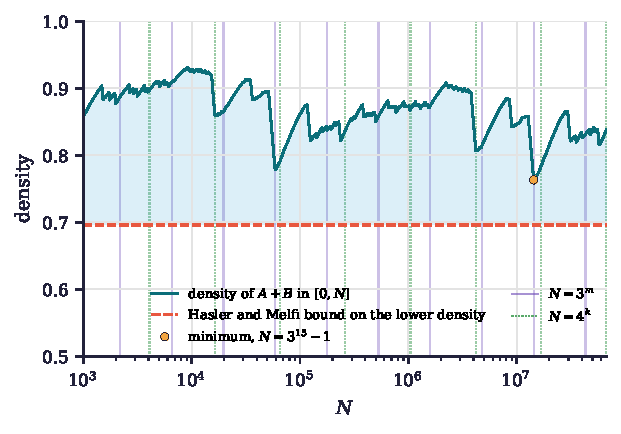
\includegraphics[width=\textwidth]{figures/ch8_erdos125.pdf}
\caption{Density of $A+B$ in $[0,N]$ for $10^3\leq N\leq4^{13}$, with
vertical lines at the powers of $3$ (solid) and of $4$ (dotted) and the Hasler and Melfi upper bound
$1015/1458$ on the lower density.}
\label{fig:ch8:erdos}
\end{figure}

Three things are visible in \cref{fig:ch8:erdos}. The density stays well above
the Hasler and Melfi bound throughout the range, so finite computation gives
no hint that the lower density is zero: the decay that the proof exploits
operates at the scale of the good approximations to $2/\theta$, and the first
very good one, $3^{53}\approx4^{42}$, is far beyond any computation. The
minima sit just below powers of $3$, where a new block of $A$ is about to
begin and the previous blocks have been exhausted. And the deepest dips occur
when a power of $3$ lies a little below a power of $4$: $3^{10}/4^{8}=0.90$
and $3^{15}/4^{12}=0.855$ are such cases, and they give the two lowest values
in the table. This is the thinning mechanism of the proof seen at small scale:
when $3^m$ and $4^k$ are close, the two digit structures align, and the gaps
of $A$ and of $B$ overlap rather than fill each other.

\subsection{The analogy}

Both problems turn on good rational approximations to a ratio of logarithms, but they use them in opposite ways.
For Erd\H{o}s $125$ the coincidences are $3^m\approx4^k=2^{2k}$, that is, approximations $2k/m$ to $\theta$ from either side; they produce windows in which $A+B$ thins, and the proof uses infinitely many such windows to drive the lower density to zero.
Only their existence matters, and it follows from soft arguments, such as the pigeonhole principle or \cref{lem:ch8:basic}; the example $3^{53}\approx4^{42}$ is the convergent $84/53$, which lies below $\theta$ and is useless for cycles (\cref{rem:ch8:false}).
For Collatz cycles the good approximations $3^r\approx2^s$ with $s/r$ just above $\theta$ are exactly what a cycle needs; their records bound the length of a cycle (\cref{thm:cycles}), but by \cref{prop:ch8:insufficient} they are good enough infinitely often, whatever the verification range, so no information about the approximations of $\theta$ alone, not even bounded partial quotients, can exclude every cycle.
In one problem the existence of good approximations is the engine of the proof; in the other it is an obstruction that Diophantine\index{Diophantine approximation} approximation cannot remove, and what is missing is arithmetic information about the parity word (\cref{cor:ch8:window}).
That asymmetry is a fair summary of why the cycle half is hard.

\section{Machine checked statements}\label{sec:ch8:lean}

A bound such as \cref{thm:cycles} is assembled from a short chain of
elementary steps and a finite computation, which makes it an attractive
target for formal verification. In our note~\cite{polsonsokolov2026nexus} we
wrote two small files in Lean\index{Lean}~4~\cite{moura2021}, using only the core library
(Lean 4.15, without Mathlib). The restriction is severe: there are no real
numbers, no rationals and no limits, so every statement must be phrased in
natural number arithmetic, and every proof uses only induction, case
analysis, linear arithmetic and the kernel. It is also useful, since it
forces exactly the logarithm free formulations a verified cycle bound will
need. Both files compile; the first produces no warnings, the second one
warning for each open statement. They are in the folder \texttt{lean} of the book's repository (\cref{app:code}).

\lstdefinestyle{ch8lean}{language={},basicstyle=\ttfamily\scriptsize,literate={→}{{$\to$}}1 {∃}{{$\exists$}}1 {∀}{{$\forall$}}1 {∧}{{$\land$}}1 {∨}{{$\lor$}}1 {¬}{{$\neg$}}1 {≤}{{$\le$}}1 {≥}{{$\ge$}}1}

\subsection{What is proved}

The definitions are the accelerated map\index{accelerated map}, its iterates and the number of odd
steps.

\begin{lstlisting}[style=ch8lean]
def T (x : Nat) : Nat :=
  if x % 2 = 0 then x / 2 else (3 * x + 1) / 2
def Tn : Nat → Nat → Nat
  | 0, x => x
  | k + 1, x => T (Tn k x)
def odd : Nat → Nat → Nat
  | 0, _ => 0
  | k + 1, x => odd k x + (if Tn k x % 2 = 1 then 1 else 0)
\end{lstlisting}

\noindent The four theorems are the following.

\begin{lstlisting}[style=ch8lean]
theorem B1 (k x : Nat) : ∃ c : Nat,
    2 ^ k * Tn k x = 3 ^ (odd k x) * x + c ∧
    (odd k x > 0 → c > 0)
theorem B2 {k x : Nat} (hx : x > 0) (hk : k > 0)
    (hcyc : Tn k x = x) (ho : odd k x > 0) :
    3 ^ (odd k x) < 2 ^ k
theorem B3 : ∀ x, 1 ≤ x → x ≤ 10000 →
    ∃ j, j ≤ 400 ∧ Tn j x = 1
theorem B4 : Tn 1 1 = 2 ∧ Tn 2 1 = 1 ∧
    ∀ k, Tn k 1 = 1 ∨ Tn k 1 = 2
\end{lstlisting}

B1 is the affine identity of \cref{prop:ch2:affine}, proved by induction on
$k$ through a stronger lemma that names the remainder by the explicit
recursion $c_{k+1}=3c_k+2^k$ after an odd step and $c_{k+1}=c_k$ after an even
one; an inductive hypothesis asserting only the existence of some remainder is
awkward to propagate. B2 is the cycle inequality $3^m<2^k$ of
\cref{cor:ch2:cycle}, the lower half of \eqref{eq:ch8:theta}. B3 checks that
every starting value from $1$ to $10^4$ reaches $1$ within $400$ steps of $T$
(the true maximum is $165$ steps, at $x=6171$, by our own count). It starts at
$x=1$ because $0$ is a fixed point of $T$, so the statement over all
$x\leq10^4$ would be false. It is proved by a Boolean evaluator together with
a kernel checked soundness lemma, and the evaluation is run natively rather
than in the kernel, so the proof depends on the axiom
\texttt{Lean.ofReduceBool}, which amounts to trusting the compiled evaluator.
B4 describes the trivial cycle. The axiom report printed by Lean\index{Lean} is: B1 uses
\texttt{propext} and \texttt{Quot.sound}; B2 also uses
\texttt{Classical.choice}; B3 uses \texttt{propext}, \texttt{Quot.sound} and \texttt{Lean.ofReduceBool}; B4 uses no
axioms. The proofs were written by an AI coding agent working against the
compiler, and we then recompiled both files independently and read every
statement against its informal meaning, which is where the two details just
mentioned were caught.

\subsection{What is stated}

The open statements are the conjecture, its descent form, and the cycle
problem.

\begin{lstlisting}[style=ch8lean]
theorem O1_collatz : ∀ x, x ≥ 1 → ∃ k, Tn k x = 1
theorem O3_descent : ∀ x, x ≥ 2 → ∃ k, k > 0 ∧ Tn k x < x
theorem O4_no_cycles : ¬ ∃ x k, x > 2 ∧ k > 0 ∧ Tn k x = x
\end{lstlisting}

\noindent The names O1, O3 and O4 are those of the Lean files and are unrelated to the numbering of the problems in \cref{chap:open}.
O3 implies O1 by strong induction, and O1 implies O3 because an orbit that
reaches $1$ passes below its starting value. O4 excludes every cycle of
positive integers other than $\{1,2\}$; the hypothesis $x>2$ rules out the
elements of the trivial cycle, and $x=0$ is excluded with them.

\subsection{From statements to a verified cycle bound}

What separates these files from a verified form of \cref{thm:cycles} is the
upper half of \eqref{eq:ch8:theta} and the continued fraction\index{continued fraction} computation.
Both are within reach of the core library once they are stated without
logarithms. For the first, if every element of a cycle of $T$ with $k$ steps
and $m$ odd steps is at least $X$, then by \eqref{eq:ch8:prod}
\[
  2^k=\prod_{i=1}^{m}\Bigl(3+\frac1{x_i}\Bigr)\leq\Bigl(3+\frac1X\Bigr)^m,
  \quad\text{that is}\quad 2^k(3X)^m\leq3^m(3X+1)^m,
\]
an inequality between natural numbers which, combined with B2, is the whole
content of \cref{lem:cycleid} and \cref{cor:ch8:excl}.

For the second, the exclusion of all $m<r_*(X)$ can be replaced by the short
certificate\index{certificate} of \cref{sec:ch8:certificate}. The proof of \cref{thm:cycles}(ii) uses three ingredients: the
identities of \cref{lem:ch8:basic}(ii) for the listed pairs $(p_i,q_i)$ of convergents, which
are integer arithmetic; the signs of $q_i\theta-p_i$, which are comparisons
between $3^{q_i}$ and $2^{p_i}$; and, at each rung $u$, the inequality
$\delta(u)\geq u\varepsilon$. Checking a comparison such as
$3^{q}$ against $2^{p}$ for $q$ near $10^{11}$ by direct exponentiation is
out of the question, but interval arithmetic on rational approximations of
$\lt$, proved once, reduces each check to arithmetic on integers of modest
size, as in Steps 1 to 4 of \cref{sec:ch8:certificate}; since the quantities $\delta(u)$ involved are of order $10^{-11}$ and
the margins are at least a factor $1.36$, a rational enclosure of $\lt$ to a
few dozen digits suffices.
The mediant lemma\index{mediant lemma} and \cref{thm:ch8:onesided} keep the certificate short: instead of checking $\delta(m)\geq m\varepsilon$ for each of the some $7\times10^{10}$ values $m<r_*$, \cref{cor:ch8:firstfeasible} and the lattice argument of
\cref{thm:ch8:onesided} reduce the task to the $44$ rungs up to
$r_*(2^{68})$, and there are only $53$ rungs below $2\times10^{13}$ in all.
This is a well posed task for an automated prover of the AlphaProof Nexus\index{AlphaProof Nexus}
type, and it would make the cycle bound the first part of the programme of
this book to be fully machine checked. The remaining trusted input would be
the verification range\index{verification range} itself, which rests on a large computation of a
different kind.

\section{A refined open problem}\label{sec:ch8:refined}

The cycle length bounds above use the cycle structure only through the crude inequality $\log(1+1/(3x_i))\leq1/(3M)$, and the window lemma adds only the lower bound $c_k\geq3^m-2^m$.
For any cycle with $m$ odd steps, $k$ steps in all and smallest element $x_{\min}$, \cref{lem:ch8:window} gives
\[
  x_{\min}<\frac{m}{3\Lambda}\le\frac{m}{3\log2\;\delta(m)},\qquad\Lambda=k\log2-m\log3 .
\]
The remaining information in a cycle lies in its parity vector\index{parity vector}. A cycle of $T$
is described by a word of length $k$ with $m$ ones, and by
\cref{cor:ch2:cycle} each element is $x=c_k(x)/(2^k-3^m)$, where the affine
constant $c_k(x)$ of \eqref{eq:ch2:cexplicit} is a sum of terms $3^{j}2^{i}$
indexed by the positions of the ones in the word. The thinning argument of the
Erd\H{o}s $125$ proof controls how two digit expansions interact over a window
in which $3^m\approx4^k$, and it is natural to ask whether a similar block
decomposition of the parity word can be brought to bear here.

\begin{problem*}[Arithmetic sharpening of the cycle identity]
Find a function $f$, derived from the arithmetic of the parity vector rather
than from the size of the elements, such that every nontrivial cycle with $m$
odd steps and $k$ steps in all satisfies
\[
  x_{\min}<\frac{m}{3\Lambda\,f(m)},\qquad\Lambda=k\log2-m\log3 .
\]
By \cref{cor:ch8:window}, any $f$ with $f(m)\geq\frac m3(1+\eta)$ for large $m$ would confine the least element of every nontrivial cycle with many odd steps below about $1/(2\eta)$, and so reduce the cycle half to a finite verification; one may also try to raise the lower end $(1-(2/3)^m)/(e^{\Lambda}-1)$ of the window by a factor slightly more than $m/3$, which would empty the window whenever $\Lambda$ is small.
More concretely: does a block decomposition of the parity word, in
the style of the thinning argument for Erd\H{o}s $125$, force $c_k(x)$ to be
large compared with $3^m-2^m$, or constrain it modulo $2^k-3^m$, in a way that
the size of $x$ alone does not?
\end{problem*}

The target is demanding. For balanced words\index{balanced words} the least element already sits at
about $0.72$ of the upper end of the window, so no size argument can gain the
factor $m/3$ there, and the exploration of parity words found residues
$c_k(w)\bmod(2^k-3^m)$ behaving like uniform random variables. A proof along
these lines must therefore exploit divisibility, and would amount to showing
that $2^k-3^m$ never divides $c_k(w)$ except for the trivial word. Any partial
result with $f$ bounded below by a constant $b>1$ would lower every threshold of \cref{tab:ch8:thresholds} by at least the factor $b$, which is worth at least as much as a verification range larger by the factor $b$, at every range at once; a result with $f(m)\to\infty$ would eventually gain more than any fixed increase of the verification range. We collect the problem, with the others raised in the book, in
\cref{chap:open}.

\section*{Notes}

The cycle identity\index{cycle identity} and the bound $M<r/(3\Lambda_r)$ go back at least to the
1970s; the use of continued fractions\index{continued fraction} of $\lt$ for cycle bounds is due to
Crandall\index{Crandall, R. E.}~\cite{crandall1978}, whose criterion is in substance the block bound of \cref{lem:block}, to
Steiner\index{Steiner, R. P.}~\cite{steiner1977} and, with larger verification ranges\index{verification range}, to
Eliahou\index{Eliahou, S.}~\cite{eliahou1993}. The surveys of Lagarias\index{Lagarias, J. C.}~\cite{lagarias1985} and
the collection~\cite{lagarias2010} describe the history, including the
negative cycles\index{negative cycles} and the $3x-1$ problem, and Lagarias~\cite{lagarias1990}
treats the rational cycles\index{rational cycles}. Simons and de Weger~\cite{simons2005} and
Hercher\index{Hercher, C.}~\cite{hercher2023} are the current state of the art for $m$ cycles
and for the length bound, Hercher's record~\cite[Corollary~29]{hercher2023} being unconditional since the verification to $2^{71}$. The verification ranges $2^{68}$ and $2^{71}$ are due to
Ba\v{r}ina\index{Barina, D.@Ba\v{r}ina, D.}~\cite{barina2021,barina2025}; see also the account of earlier verification
efforts in~\cite{lagarias2010}. For continued fractions,
Khinchin~\cite{khinchin1964} remains the most economical introduction, Hardy
and Wright~\cite{hardywright2008} give the best approximation theorems, and
Rockett and Sz\"usz~\cite{rockett1992} treat one sided approximation\index{one sided approximation} and the
role of the intermediate fractions\index{semiconvergent}. Linear forms in two logarithms are treated
by Laurent, Mignotte and Nesterenko~\cite{laurent1995}, and the general theory
by Baker~\cite{baker1975}. The record structure of \cref{prop:records} is classical, equivalent to finding
the least denominator fraction in an interval just above $\lt$ (Lemma 22 of
Hercher~\cite{hercher2023}), and is the description of the best one sided approximations that Han\v{c}l\index{Hancl, J.@Han\v{c}l, J.} and Turek\index{Turek, O.}~\cite[Theorem~4.5(ii)]{hancl2019} state and prove; the mediant lemma\index{mediant lemma} and \cref{thm:ch8:onesided} give a short self contained proof of the
part we need. Halbeisen\index{Halbeisen, L.} and Hungerb\"uhler\index{Hungerbuhler, N.@Hungerb\"uhler, N.}~\cite{halbeisen1997} give the optimal criterion, attained by the balanced parity word, and observe for Eliahou's criterion that the dangerous lengths lie between convergents, that convergents from the wrong side are harmless and that multiples tie exactly~\cite[\S4.4]{halbeisen1997}. The comparison of exact and crude bounds, the integer
certificate\index{certificate}, the threshold table, the insufficiency proposition and the window
corollary are ours, although the structural point of the insufficiency proposition is made in another form in~\cite[\S5]{halbeisen1997}; the lower bound
$c_k\geq3^m-2^m$ underlying the window is elementary and is implicit in the
classical analyses of cycles by B\"ohm\index{Bohm, C.@B\"ohm, C.} and Sontacchi\index{Sontacchi, G.}~\cite{bohm1978} and by Steiner. The Erd\H{o}s $125$ problem is from Burr, Erd\H{o}s, Graham
and Li~\cite{burr1996}, and its resolution is in Tsoukalas and
collaborators~\cite{tsoukalas2026}; the exact density computation and the Lean\index{Lean}
files are from our unpublished note~\cite{polsonsokolov2026nexus}. For Lean~4 see de Moura\index{de Moura, L.}
and Ullrich\index{Ullrich, S.}~\cite{moura2021}.

\section*{Exercises}

\begin{exercise}
Verify the cycle identity\index{cycle identity} \eqref{eq:ch8:prod} for the three negative cycles\index{negative cycles} of
\cref{tab:ch8:negative}, and show that for a cycle of negative integers the
inequality is reversed: $2^s<3^r$. Show that the conjugation $n\mapsto-n$
carries $T_0$ on the negative integers to the map $n\mapsto n/2$ ($n$ even),
$n\mapsto3n-1$ ($n$ odd) on the positive integers, and list the corresponding
cycles of this map.
\end{exercise}

\begin{exercise}
Using \eqref{eq:ch2:affine}, find the rational periodic points of $T$ whose
parity words are $(1,0)$, $(1,1,0)$, $(1,0,0)$ and $(1,1,0,0)$, and check
which of them are integers. Show that for every word $w$ with $2^k\neq3^m$ the
number $c(w)/(2^k-3^m)$ is a rational number with odd denominator whose orbit
under $T$ is periodic with parity word $w$.
\end{exercise}

\begin{exercise}
Prove that the best approximations from below, the $r$ with
$\{r\theta\}<\{r'\theta\}$ for every $1\leq r'<r$, are exactly $r=1$ and the rungs
$q_{k-1}+jq_k$ with $k\geq1$ odd and $1\leq j\leq a_{k+1}$, by adapting the proof
of \cref{thm:ch8:onesided}. List them for $\lt$ below $700$.
\end{exercise}

\begin{exercise}
Show that if $q$ is a rung and $t\geq2$ is an integer with $t\,\delta(q)<1$,
then $\delta(tq)=t\,\delta(q)$ and $F(tq)=F(q)$. Deduce directly, without the
mediant lemma\index{mediant lemma}, that $tq$ is never a strict record of $F$. Which multiples of
$q_9=15\,601$ satisfy the hypothesis?
\end{exercise}

\begin{exercise}
Show that for even $i\geq0$ one has $\delta(q_i)=1-\varepsilon_i$, so that $F(q_i)=q_i/(3(1-\varepsilon_i)\log2)$, only slightly more than $q_i/(3\log2)$, and explain the triangles of \cref{fig:ch8:records}. Then, for a cycle of $T$ with $k$ steps and $m$ odd steps all of whose elements are at least $X$, prove the logarithm free inequality $2^k(3X)^m\leq3^m(3X+1)^m$, and deduce from it and $\log(1+u)<u$ for $u>0$ that $\delta(m)<m/(3X\log2)$.
\end{exercise}

\begin{exercise}
For the Erd\H{o}s $125$ sets, prove that $|A\cap[0,3^n-1]|=|B\cap[0,4^n-1]|=2^n$
and that the number of pairs $(a,b)\in A\times B$ with $a+b\leq N$ is of order
$N^{\log2/\log3+1/2}$. Using \texttt{ch08\_erdos125.py} or your own code,
compute the density of $A+B$ in $[0,N]$ for $N=3^m-1$ and $N=4^k$ up to
$4^{10}$, and relate the depth of each dip to the ratio $3^m/4^k$ for the
nearest powers.
\end{exercise}

\begin{exercise}
Show that the lower bound of \cref{lem:ch8:window} is attained exactly by the
rotation of a parity word whose $m$ ones come first, and compute the window for
$m=2$, $k=4$. Is there an integer in it? Which rational cycle\index{rational cycles} sits at its lower
end?
\end{exercise}

\begin{exercise}
Let $\nu=2$ and suppose $|\lt-s/r|\geq c/r^2$ for all $r$. Show that the
verification range\index{verification range} $X$ then excludes exactly the $r<(3cX\log2)^{1/2}$ that the
inequality \eqref{eq:ch8:irrbound} can handle, and that \cref{prop:ch8:insufficient}
still produces infinitely many nonexcluded $r$. Conclude that bounded partial
quotients for $\lt$ would not by themselves exclude all cycles.
\end{exercise}


\chapter{The Divergence Half}\label{chap:divergence}

An orbit of the Collatz map that never reaches $1$ either enters a cycle or
grows without bound.
The previous chapter dealt with cycles: a cycle is an exact multiplicative coincidence, continued fractions\index{continued fraction} of $\lt$ control how long it would have to be, and Diophantine\index{Diophantine approximation} information alone cannot exclude it (\cref{prop:ch8:insufficient}).
This chapter deals with the other possibility. A divergent orbit is not a
coincidence at all. It is an orbit along which the halvings are, on average,
too few, and the question of whether one exists is a question about averages
along a single deterministic sequence.

The stochastic model of \cref{chap:stochastic} answers that question for an
idealized random orbit, and the answer is no: a random walk with drift\index{drift}
$\log(3/4)$ per stride does not escape. The difficulty, which has been met in
every chapter so far, is that the model describes ensembles of starting values
and the conjecture concerns each starting value separately. In this chapter
we make the gap as precise as we can. We prove a Ces\`aro identity that turns the
divergence half into a statement about the running mean of the halving
exponents (\cref{prop:cesaro}); we show that the obvious empirical test of
that statement carries no information at all; we formulate the statement that
would be needed (\cref{conj:cesaro}) and relate its threshold $\lt$ to the
momentum\index{momentum} coefficient of \cref{chap:smm}; we study the residues of Syracuse
orbits modulo powers of $3$, where the model chain, in which the halving
exponents are independent draws, can be computed
exactly (\cref{lem:ch9:mixing}); and we describe Tao\index{Tao, T.}'s theorem, which is the
deepest result in this direction, and the reason it stops short of every
integer. The chapter ends with three routes to the divergence half and the
points at which they fail.

Throughout, $x_0$ is an odd positive integer, $y_j=S^{(j)}(x_0)$ are the
successive odd iterates under the Syracuse map\index{Syracuse map}, and
\[
  k_j=\vt(3y_{j-1}+1),\qquad\bar k_N=\frac1N\sum_{j=1}^Nk_j ,
\]
so that $y_j=(3y_{j-1}+1)/2^{k_j}$.

\section{Divergent orbits and what is known}\label{sec:ch9:known}

Call the orbit of $x_0$ \emph{divergent} if $\sup_jy_j=\infty$. No divergent
orbit is known, and very little is known about what one would look like. We
collect the elementary facts.

\begin{lemma}[Divergent orbits tend to infinity]\label{lem:ch9:infinity}
If the orbit of $x_0$ is divergent, then $y_j\to\infty$, the values $y_j$ are
pairwise distinct, and no $y_j$ is an integer known to reach $1$; in
particular $y_j>2^{71}$ for all $j$.
\end{lemma}

\begin{proof}
If $y_i=y_j$ for some $i<j$, the orbit is periodic from $i$ on and hence
bounded, so the values are distinct. A sequence of distinct positive integers
takes each value at most once, so for every $B$ only finitely many $y_j$ are at
most $B$, and $y_j\to\infty$. If some $y_j$ reached $1$ the orbit would be
bounded. Every integer below $2^{71}$ reaches $1$ by the computation of
Ba\v{r}ina\index{Barina, D.@Ba\v{r}ina, D.}~\cite{barina2025}, so no $y_j$ lies below $2^{71}$, and $y_j\neq2^{71}$ since $y_j$ is odd.
\end{proof}

Beyond this, the known results about divergence are of two kinds. Density
theorems say that the set of starting values with badly behaved orbits is
small: Terras\index{Terras, R.}~\cite{terras1976,terras1979} and, independently,
Everett\index{Everett, C. J.}~\cite{everett1977} (\cref{thm:density}) show that almost every integer, in natural
density, falls below its starting value; Korec\index{Korec, I.}~\cite{korec1994} shows that
almost every orbit falls below $n^{\gamma}$ for each $\gamma>\log3/\log4$; and
Tao\index{Tao, T.}~\cite[Theorem~1.3]{tao2022} shows that, for every function $f$ tending to
infinity, almost every orbit, in logarithmic density, falls below $f(n)$. None of these statements implies that
the set of starting values with divergent orbits has density zero, let alone
that it is empty, because an orbit that falls below its starting value may rise
again, and its later values are not uniformly distributed in any residue
class. Counting theorems, of which the strongest is due to Krasikov\index{Krasikov, I.} and
Lagarias\index{Lagarias, J. C.}~\cite{krasikov2003}, give lower bounds for the number of integers that
provably reach $1$; we return to them in \cref{sec:ch9:krasikov}.

The second kind of result is structural: a divergent orbit, if one exists,
must be atypical in a precise statistical sense. The rest of this section and
the next make that precise.

\begin{remark}[The $2$ adic picture]\label{rem:ch9:adic}
By \cref{thm:ch2:conj}, the accelerated map\index{accelerated map} on the $2$ adic integers is
conjugate to the shift on parity sequences, and Haar measure\index{Haar measure} corresponds to
fair coin flips (\cref{prop:ch2:haar}). By the strong law of large numbers,
Haar almost every $2$ adic integer has a $T$ orbit in which the frequency of
odd steps is $\tfrac12$. We shall see in \cref{cor:ch9:freq} that a divergent
orbit must have a frequency of odd steps of at least $1/\lt\approx0.631$ in the
limit. The set of $2$ adic integers with this property has Haar measure zero.
This is no contradiction, since the positive integers are themselves a set of
Haar measure zero, but it is a measure of how atypical a divergent orbit must
be. Counting parity words gives a quantitative version: among the $2^n$ words
of length $n$, the number with at least $qn$ ones, $q=1/\lt$, is
$2^{nH(q)+o(n)}$, where $H(q)=-q\log_2q-(1-q)\log_2(1-q)\approx0.9500$. The
fraction of residue classes modulo $2^n$ whose first $n$ steps of $T$ contain
at least $n/\lt$ odd steps therefore decays like $2^{-0.05n}$, the rate $e^{-D}\approx
0.9659$ per step of \cref{thm:density} and \cref{sec:ch3:lyapunov}.
\end{remark}

\section{The Ces\`aro identity}\label{sec:ch9:cesaro}

The following identity is the telescoped form of the stride formula
\eqref{eq:ch2:stride}. It is elementary, and its value lies entirely in what it
does and does not say.

\begin{proposition}[Ces\`aro identity]\label{prop:cesaro}
For every odd $x_0$ and every $N\geq1$,
\begin{equation}\label{eq:ch9:cesaro}
  \log y_N-\log x_0=\sum_{j=1}^{N}\log\Bigl(3+\frac{1}{y_{j-1}}\Bigr)
  -N\bar k_N\log2 .
\end{equation}
Equivalently,
\begin{equation}\label{eq:ch9:kbar}
  \bar k_N=\lt+\frac{1}{N}\Bigl(\log_2x_0-\log_2y_N+\sum_{j=1}^{N}
  \log_2\Bigl(1+\frac{1}{3y_{j-1}}\Bigr)\Bigr).
\end{equation}
Consequently, if the orbit of $x_0>1$ reaches $1$ at stride $N$, then
\begin{equation}\label{eq:ch9:forced}
  \bar k_N\;>\;\lt+\frac{\log_2x_0}{N}\;>\;\lt .
\end{equation}
\end{proposition}

\begin{proof}
Taking logarithms in $2^{k_j}y_j=3y_{j-1}+1$ gives
$\log y_j-\log y_{j-1}=\log(3+1/y_{j-1})-k_j\log2$, and summing over
$j=1,\ldots,N$ gives \eqref{eq:ch9:cesaro}. Writing
$\log(3+1/y)=\log3+\log(1+1/(3y))$, dividing by $N\log2$ and rearranging
gives \eqref{eq:ch9:kbar}. If $y_N=1$ then $\log_2y_N=0$ and every correction
term $\log_2(1+1/(3y_{j-1}))$ is positive, which gives \eqref{eq:ch9:forced}.
\end{proof}

The identity converts the conjecture into a statement about the running mean
of the halving exponents. Its consequence for divergent orbits is the
following.

\begin{corollary}[The running mean along a divergent orbit]\label{cor:ch9:freq}
If the orbit of $x_0$ is divergent, then
\[
  \limsup_{N\to\infty}\bar k_N\;\le\;\lt .
\]
Equivalently, the fraction of odd steps among the first $n$ steps of the
accelerated map\index{accelerated map} satisfies $\liminf_n(\text{fraction})\geq1/\lt\approx0.6309$,
and among the first $n$ steps of the standard map\index{standard map}
$\liminf_n(\text{fraction})\geq1/(1+\lt)\approx0.3869$.
\end{corollary}

\begin{proof}
By \cref{lem:ch9:infinity}, $y_j\to\infty$, so the correction terms
$\log_2(1+1/(3y_{j-1}))$ tend to zero and so does their Ces\`aro mean; and
$\log_2y_N>0$ for all large $N$. Inserting both facts in \eqref{eq:ch9:kbar}
gives $\bar k_N\le\lt+o(1)$. The first $N$ strides contain $N$ odd steps and
$N\bar k_N$ steps of $T$, or $N(1+\bar k_N)$ steps of $T_0$. If step $n$ of
$T$ falls in stride $N+1$, then at least $N$ of the first $n$ steps are odd and
$n\le(N+1)\bar k_{N+1}\le(N+1)(\lt+o(1))$, so the fraction of odd steps is at
least $N/((N+1)(\lt+o(1)))$, which tends to $1/\lt$. The same count with
$1+\bar k_{N+1}$ in place of $\bar k_{N+1}$ gives the statement for $T_0$.
\end{proof}

The typical values are $\bar k_N\to2$, an odd fraction of $\tfrac12$ for $T$
and $\tfrac13$ for $T_0$ (\cref{prop:ch3:standard}). A divergent orbit must
sustain more than $63$ percent odd steps under $T$, against a typical $50$.

\subsection{A pitfall: the identity is not a test}

Since a divergent orbit must have $\limsup\bar k_N\le\lt$, it is natural to
compute $\bar k_N$ along many orbits and observe that it stays above $\lt$.
The computation is easy and the result is striking.

\begin{remark}[A tempting but uninformative computation]\label{rem:ch9:circular}
For all $2500$ odd starting values $3\le x_0\le5001$ we computed $\bar k_N$ at
the stride $N$ at which the orbit reaches $1$. The minimum is $1.7073$, the
mean is $2.2473$, and every value lies above the threshold $\lt=1.5850$; the
identity \eqref{eq:ch9:cesaro} holds along every orbit with a maximum rounding
residual of about $3\times10^{-14}$. One might present this as evidence
for the divergence half. It is not evidence of any kind. The orbits in the scan
were selected by the property that they reach $1$, and by
\eqref{eq:ch9:forced} every such orbit satisfies $\bar k_N>\lt$ identically.
No outcome of the computation could have been different. The minimum $1.7073$
is $70/41$, attained at $x_0=27$ (\cref{ex:ch2:27}), and it measures the spread
of $\bar k$ over terminating orbits; it says nothing about orbits that do not
terminate.
\end{remark}

The same lesson appears in a sharper form for long orbits. For three odd
starting values chosen at random near $2^{1000}$, $2^{2000}$ and $2^{4000}$, the
orbits reached $1$ after $N=2773$, $4566$ and $9507$ strides, with final means
$\bar k_N=1.94555$, $2.02300$ and $2.00568$. By \eqref{eq:ch9:kbar} with
$y_N=1$, these are
\[
  \bar k_N=\lt+\frac{\log_2x_0}{N}+\frac1N\sum_{j}\log_2\Bigl(1+\frac1{3y_{j-1}}\Bigr),
\]
and the last term is below $10^{-4}$ in all three cases; the values of
$\lt+(\log_2x_0)/N$ are $1.94547$, $2.02293$ and $2.00565$. So the final mean
of the halving exponents carries no information beyond the number of strides,
which is itself a reformulation of the total stopping time\index{stopping time}. What does carry
information is the behaviour of $\bar k_N$ along the way, at strides $N$ when
the orbit is still far from $1$, and that is what \cref{fig:ch9:kbar} shows.

\begin{figure}[t]
\centering
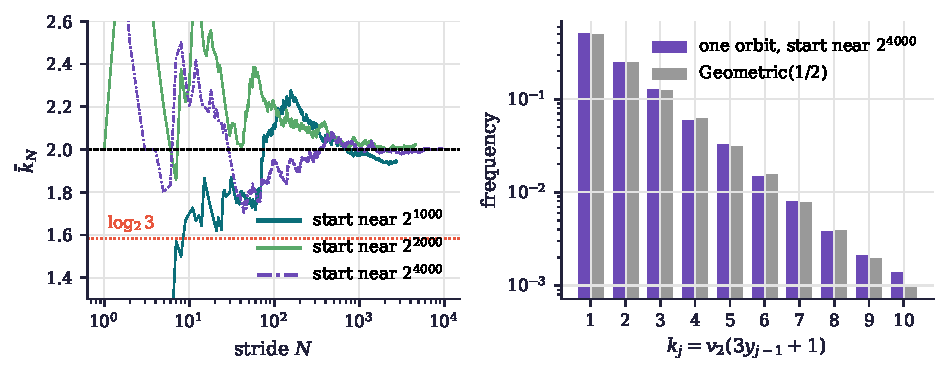
\includegraphics[width=\textwidth]{figures/ch9_kbar.pdf}
\caption{Left: the running mean $\bar k_N$ along three orbits started at random
odd integers near $2^{1000}$, $2^{2000}$ and $2^{4000}$, with the Geometric mean
$2$ (dashed) and the threshold $\lt$ (dotted). Right: the frequencies of the
halving exponents along the orbit from near $2^{4000}$ against the
Geometric$(\tfrac12)$ law, on a logarithmic scale.}
\label{fig:ch9:kbar}
\end{figure}

\section{The Ces\`aro liminf conjecture}\label{sec:ch9:conj}

The divergence half of the conjecture can now be stated in the form the
identity suggests.

\begin{conjecture}[Ces\`aro liminf]\label{conj:cesaro}
For every odd $x_0$,
\[
  \liminf_{N\to\infty}\frac1N\sum_{j=1}^Nk_j\;>\;\lt .
\]
\end{conjecture}

\begin{sloppypar}
Along an orbit that reaches $1$ the exponents are eventually all equal to $2$, since $S(1)=1$ with $k=2$, and along an orbit that enters a cycle with $r$ odd elements and $s$ halvings in one turn their mean tends to $s/r>\lt$ (\cref{lem:cycleid}); so \cref{conj:cesaro} holds for every bounded orbit.
By \cref{cor:ch9:freq}, every divergent orbit has $\liminf\bar k_N\le\limsup\bar k_N\le\lt$, so \cref{conj:cesaro} holds if and only if there is no divergent orbit.
It is therefore exactly equivalent to the divergence half of
the Collatz conjecture\index{Collatz conjecture}, and its interest lies not in being weaker but in
pointing at a mechanism. Under the Geometric law of \cref{prop:geom} the
exponent at a uniformly random odd residue has mean $2$, and if the exponents along an orbit obeyed the strong
law of large numbers we would have $\bar k_N\to2>\lt$, with a margin of
$2-\lt\approx0.415$. The margin belongs to the model: along a divergent orbit there is none, by \cref{cor:ch9:freq}.
A proof of \cref{conj:cesaro} would need much less than a Geometric law for the exponents along unbounded orbits, or full equidistribution\index{equidistribution} of their residues (\cref{sec:ch9:equi}): one needs only that along no orbit $\limsup_N\bar k_N\le\lt$, that is, that the mean of the exponents cannot fall short of $2$ by $2-\lt\approx0.415$ or more in the limit.
\end{sloppypar}

The threshold has a second reading. Write
\[
  \lt=1+\beta,\qquad\beta=\frac{\log(3/2)}{\log2}\approx0.585 ,
\]
where $\beta$ is the Switching MM\index{Switching MM} momentum\index{momentum} coefficient of \cref{chap:smm}. Every
stride contains one forced halving, since $k_j\geq1$, and the conjecture
asks that the \emph{extra} halvings $k_j-1$ exceed $\beta$ on average. In the
optimization reading of the book, the tripling and the forced halving together
form the overshoot $\log(3/2)$, and $\beta$ is that overshoot measured in units
of one halving; the extra halvings are the corrective descent. The Geometric
law gives $\E[k-1]=1$, so the correction exceeds the overshoot by a factor
$1/\beta\approx1.71$. The divergence half asks that this inequality, which
holds in expectation, hold along every orbit in the long run.

\section{Equidistribution of the halving exponent along orbits}\label{sec:ch9:equi}

The right panel of \cref{fig:ch9:kbar} shows the empirical law of $k_j$ along
the single orbit from near $2^{4000}$. Over its $9507$ strides the frequencies
of $k=1,2,3,4,5$ are $0.5026$, $0.2462$, $0.1271$, $0.0596$, $0.0330$, against
$0.5$, $0.25$, $0.125$, $0.0625$, $0.03125$; the sample mean is $2.0057$ and the
sample variance $2.0913$, against $2$ and $2$. The running means in the left
panel settle near $2$ and stay well clear of $\lt$ once the orbit is past its
first few dozen strides.

Part of this agreement is a theorem and part of it is not. Extending
\cref{prop:ch3:exact} to strides: if $x_0$ is uniformly distributed over the odd
residues modulo $2^K$, the parity vector\index{parity vector} of length $K$ is uniform over the words that begin with $1$, so the
halving exponents $k_1,k_2,\ldots$ are independent Geometric$(\tfrac12)$ for
as long as their sum stays below $K$. A starting value near $2^{4000}$ thus
controls roughly the first $2000$ strides, about a fifth of its orbit. After
that the exponents are determined by bits that the orbit has manufactured
itself, through the multiplications by $3$ and the additions of $1$, and no
theorem says they remain Geometric.
The figure says that they do, and so do the other long orbits computed in this book, such as the giant orbit of the gallery (Plate~\ref{fig:gal:giant}); this is the phenomenon that has never been proved.
Note also that the theorem concerns an ensemble of starting values,
whereas the figure shows one orbit. Even over the first $2000$ strides,
\cref{prop:ch3:exact} says only that most residue classes produce Geometric
statistics, not that the particular orbit drawn does.
The same is true of the quantitative form due to Tao\index{Tao, T.}, which shows that the first halving exponents of a starting value drawn at random from a long range are close in total variation to independent Geometric$(\tfrac12)$ draws~\cite[Proposition~1.9]{tao2022}.

What one would like is a statement of the form: for every odd $x_0$ whose orbit is divergent, and every $m$, the residues $y_j\bmod2^m$ are asymptotically equidistributed\index{equidistribution} over the odd classes in the Ces\`aro sense. Since $y_{j-1}\bmod2^m$ determines $\min(k_j,m)$, \cref{prop:geom} would then give $\liminf_N\bar k_N\ge2-2^{1-m}$ for every $m$, so $\liminf_N\bar k_N\ge2$ along such an orbit, against $\limsup_N\bar k_N\le\lt$ from \cref{cor:ch9:freq}; the statement is therefore equivalent to the divergence half, as \cref{conj:cesaro} is. It cannot be asked of every orbit: an orbit that reaches $1$ stays there, so its residues are eventually constant and are not equidistributed for any $m\geq2$. For orbits that reach $1$ the natural statement concerns random starting values, as problem O2 of \cref{chap:open} does for the residues modulo $3^a$.

\section{The $3$ adic side: the model chain modulo $3^a$}\label{sec:ch9:spectral}

The $2$ adic residues of the iterates determine the halving exponents; the
$3$ adic residues are where the multiplication by $3$ leaves its mark, and it
is on the $3$ adic side that Tao\index{Tao, T.} found the leverage for his theorem. Here the
picture is clean enough to compute exactly.

Since $3y+1\equiv1\pmod3$ and $2$ is invertible modulo $3$, every Syracuse
iterate $S(y)$ is prime to $3$. Fix $a\geq1$ and $M=3^a$, and let $U_a$ be the
set of $2\cdot3^{a-1}$ units modulo $M$. For $r\in U_a$ define the matrix
\begin{equation}\label{eq:ch9:P}
  P_a(s,r)=\sum_{k\geq1}2^{-k}\,\mathbb{I}\bigl[(3r+1)2^{-k}\equiv s\pmod M\bigr],
  \qquad r,s\in U_a ,
\end{equation}
in which $\mathbb{I}$ is the indicator function, $2^{-k}$ inside it denotes the inverse of $2^k$ modulo $M$, and the weight $2^{-k}$ in front of it is the real number. Column $r$ of $P_a$
is the law of $S(y)\bmod M$ when $y\equiv r\pmod M$ and the halving exponent is
an independent Geometric$(\tfrac12)$ variable.

\begin{lemma}[The one step matrix is exact]\label{lem:ch9:exact}
For each $r\in U_a$ and $s\in U_a$,
\[
  \lim_{X\to\infty}\frac{\#\{y\le X:\ y\text{ odd},\ y\equiv r,\ S(y)\equiv s\pmod M\}}
  {\#\{y\le X:\ y\text{ odd},\ y\equiv r\pmod M\}}=P_a(s,r).
\]
More generally, for each fixed $J$, as $X\to\infty$ the joint law of
$(y\bmod M,k_1,\ldots,k_J)$ for $y$ uniform over the odd integers up to $X$
converges to the product of the uniform law and $J$ independent
Geometric$(\tfrac12)$ laws.
\end{lemma}

\begin{proof}
Fix exponents $k_1,\ldots,k_J$ with sum $s_J$. By \cref{thm:terras} (in its
Syracuse form, of which \cref{prop:geom} is the one stride case), the odd $y$ with these exponents form a
single residue class modulo $2^{s_J+1}$. By the Chinese remainder theorem its
intersection with a class modulo $3^a$ is a single class modulo
$2^{s_J+1}3^a$, whose density among the odd integers is
$2^{-s_J}\cdot3^{-a}$. This is the product law. Given $k_1=k$ and
$y\equiv r$, the residue of $S(y)=(3y+1)2^{-k}$ modulo $M$ is
$(3r+1)2^{-k}$, which gives the first statement.
\end{proof}

So the one step transition frequencies are not a model: they are exact
limits. A model enters only when the matrix is iterated, since iterating
assumes that the exponent at each stride is independent of the current residue and of the past along the
orbit. We call the Markov chain on $U_a$ with transition matrix $P_a$, in which the halving exponents are independent Geometric$(\tfrac12)$ draws at every stride, the \emph{model chain}.
By the second half of \cref{lem:ch9:exact} its assumption is again
exact for an ensemble of starting values over any fixed number of strides,
and the residues $y_j\bmod M$ for a uniformly random large $y_0$ then form,
in the limit, a Markov chain with transition matrix $P_a$. For a single orbit
nothing of the kind is known: along an orbit the exponents are determined by the iterates, and the Syracuse map does not induce a Markov chain on residues modulo $M$.

\begin{lemma}[Exact mixing in $a$ strides]\label{lem:ch9:mixing}
For $0\le j\le a$, column $r$ of $P_a^{\,j}$ depends on $r$ only through
$r\bmod3^{a-j}$. In particular $P_a^{\,a}=\pi_ae^{\top}$, where $e$ is the vector of ones: all columns of $P_a^{\,a}$ equal
the stationary law $\pi_a$ of $P_a$, so the model chain is exactly stationary after $a$ strides from every starting residue.
Consequently the eigenvalue $1$ of $P_a$ is simple and every other eigenvalue is zero: the characteristic polynomial of $P_a$ is $\lambda^{|U_a|-1}(\lambda-1)$.
\end{lemma}

\begin{proof}
Let $K_1,K_2,\ldots$ be independent Geometric$(\tfrac12)$ and define the random
map $\phi_i(r)=(3r+1)2^{-K_i}\bmod M$. By induction,
\[
  \phi_j\circ\cdots\circ\phi_1(r)\equiv3^j2^{-(K_1+\cdots+K_j)}r+c_j\pmod M,
\]
where $c_j$ depends on $K_1,\ldots,K_j$ only. The first term depends on $r$ only
through $r\bmod3^{a-j}$, and vanishes modulo $M$ for $j=a$. Column $r$ of
$P_a^{\,j}$ is the law of this composition, which proves the first two claims.
The matrix $P_a^{\,a}=\pi_ae^{\top}$ has rank one and trace $e^{\top}\pi_a=1$, so its eigenvalues, counted with multiplicity, are $1$ once and $0$ otherwise.
They are the $a$th powers of the eigenvalues of $P_a$, and $1$ is an eigenvalue of $P_a$ because $e^{\top}P_a=e^{\top}$; hence $1$ is simple and every other eigenvalue of $P_a$ is zero.
\end{proof}

The identity in the proof is Tao\index{Tao, T.}'s~\cite[eq.~(1.21)]{tao2022}: the residue of the $m$th Syracuse iterate modulo $3^a$ depends only on the halving exponents once $m\geq a$. His recursion~\cite[Lemma~1.12]{tao2022} is one step of the model chain, and he notes that the law of his Syracuse random variable is the unique stationary measure of the $3$ adic chain $x\mapsto(3x+1)/2^k$ with $\Prob(k)=2^{-k}$~\cite[Remark~1.13]{tao2022}. What \cref{lem:ch9:mixing} adds is a restatement in the form of a finite Markov chain, $P_a^{\,a}=\pi_ae^{\top}$, from which the spectrum follows. The order matters: the converse inference fails, since a zero spectrum off the eigenvalue $1$ only makes $P_a-\pi_ae^{\top}$ nilpotent, which by itself would allow the chain as many as $|U_a|-1$ strides to become stationary. Nor does the proof use the law of the halving exponents beyond their independence of the current residue; that independence is the model's assumption, and it fails along an actual orbit, where the exponents are determined by the iterates.

The stationary law $\pi_a$ is the law of the \emph{Syracuse random variable}
\[ \sum_{m=1}^{a}3^{m-1}2^{-(K_1+\cdots+K_m)}\bmod3^a \] of Tao~\cite[eq.~(1.22)]{tao2022}, written in the index reversed form of~\cite[Remark~1.13]{tao2022}; the
reversal of the order of the $K_i$ relative to the proof does not change the
law. For $a=1$ it is $(\tfrac13,\tfrac23)$ on the residues $1,2$, since
$S(y)\equiv2^{-k}\equiv2^k\pmod3$ and $k$ is odd with probability $\tfrac23$.
For $a=2$, on the residues $1,2,4,5,7,8$ modulo $9$, it is
\[
  \pi_2=\tfrac1{63}\,(8,\;16,\;11,\;4,\;2,\;22).
\]
These laws are far from uniform, and the distance from uniform does not
shrink with $a$: the total variation distance from $\pi_a$ to the uniform law
on $U_a$ is $0.278$, $0.346$, $0.371$, $0.389$, $0.399$, $0.407$ for
$a=2,\ldots,7$.
For $a=3$ the most likely unit, $26$, is $29$ times as likely as the least likely, $25$; only $5$ of the $18$ units have probability within a factor $\tfrac32$ of $\tfrac1{18}$, and the median probability is $0.038$, against the mean $\tfrac1{18}\approx0.056$. Tao states that his Syracuse random variables are not uniformly distributed (\cite[Remark~1.15]{tao2022} and the paragraph before his Proposition~1.14); what he proves is approximate uniformity at fine $3$ adic scales (\cref{sec:ch9:tao}).

\begin{figure}[t]
\centering
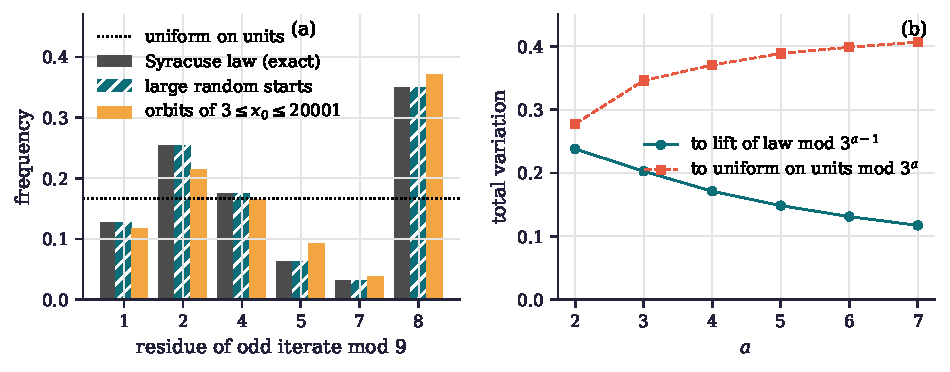
\includegraphics[width=\textwidth]{figures/ch9_syrlaw.pdf}
\caption{Left: frequencies of the residues modulo $9$ of odd Syracuse iterates, against the exact Syracuse law $\pi_2$ and the uniform law on units (dotted). In each group of three bars, the left bar is $\pi_2$, the middle bar $3000$ random starting values near $2^{511}$, strides $3$ to $102$, and the right bar all odd iterates of the orbits of $3\le x_0\le20001$, pooled over orbits that share their tails. Right: total variation distance from $\pi_a$ to the lift of $\pi_{a-1}$ (circles) and to the uniform law on units modulo $3^a$ (squares).}
\label{fig:ch9:syrlaw}
\end{figure}

\Cref{fig:ch9:syrlaw} compares $\pi_2$ with residue frequencies along actual
orbits. For $3000$ random starting values near $2^{511}$, using strides $3$ to
$102$, the empirical law is within total variation $0.0009$ of $\pi_2$; this is
a regime in which \cref{lem:ch9:exact} applies, and the agreement is a theorem
up to sampling error. For the orbits of the small odd starting values
$3\le x_0\le20001$, run to $1$, the distance is $0.058$; but these orbits share
their tails, so their pooled counts are not samples from the model law: their
roughly $317\,000$ odd iterates take only about $12\,000$ distinct values, and
$94$ percent of the orbits end with the same final stride, from $5$ through $16$ to $1$.

\begin{remark}[A pitfall: the wrong null hypothesis]\label{rem:ch9:null}
It is natural to test the $3$ adic equidistribution\index{equidistribution} of Collatz orbits by
comparing residue frequencies modulo $9$ with the uniform law on the six units,
or worse on all nine residues, with a chi squared test.
Such a test rejects decisively for every long orbit in this chapter, and the rejection means nothing.
Residues divisible by $3$ never occur after the first stride, and the correct
null hypothesis on the units is the Syracuse law $\pi_2$, which puts weight
$22/63\approx0.35$ on the residue $8$ and $2/63\approx0.03$ on the residue $7$.
Equidistribution in the sense that matters for Tao's theorem is
equidistribution with respect to the Syracuse law, not with respect to Haar
measure on the units.
\end{remark}

\subsection{A pitfall: odd representatives modulo $27$}

Since every Syracuse iterate is odd, one might build the chain modulo $27$ on the nine odd representatives
\[
  1,\ 5,\ 7,\ 11,\ 13,\ 17,\ 19,\ 23,\ 25
\]
of the units in $[1,27)$, recording a transition $r\to s$ whenever an odd $y\equiv r$ has
$S(y)\equiv s\pmod{27}$ with both $r$ and $s$ in this set. The resulting matrix appears to have a respectable spectral gap, and it is worth seeing why the gap means nothing.

\begin{remark}[A spurious spectral gap]\label{rem:ch9:oddreps}
Let $\hat P$ be the empirical transition matrix of the nine state chain just described, estimated from all odd $y\le10^6$ not divisible by $3$, with each column normalized to sum to one. Its eigenvalue of second largest modulus has modulus $0.5198$, and the limiting matrix, obtained by restricting $P_3$ of \eqref{eq:ch9:P} to the nine states and renormalizing its columns, has a complex conjugate pair of eigenvalues of modulus $0.5202$; taken at face value, this is a spectral gap\index{spectral gap} of about $0.48$. It is not the mixing rate of the model chain, nor of anything else attached to the dynamics. Since $27$ is odd, every residue class modulo $27$ contains integers of both parities, so whether the representative of $y$ in $[0,27)$ is odd says nothing about $y$, and the set of odd $y$ with odd representatives is not invariant under $S$: $55\equiv1\pmod{27}$, while $S(55)=83\equiv2\pmod{27}$. The restricted matrix conditions, at every stride, on a set that the dynamics leaves, and its eigenvalues are artefacts of the conditioning. The model chain is $P_3$ on all eighteen units, which by \cref{lem:ch9:mixing} is exactly stationary\index{mixing} after three strides, so that its eigenvalues other than $1$ are all zero.
\end{remark}

The empirical and limiting values agree, as they must, since by \cref{lem:ch9:exact} the empirical matrix converges to the restricted limiting matrix; the agreement shows only that the restricted matrix has been computed correctly. \Cref{tab:ch9:moduli} compares the restricted matrices with the model chains for the moduli $9$, $27$, $81$ and $243$.

\begin{table}[t]
\centering
\caption{Transition matrices on residues modulo $3^a$. Left block: the matrix restricted
to odd representatives, second eigenvalue modulus from the empirical matrix
(odd $y\le10^6$) and from the limiting matrix. Right block: the model chain on
all units; rank of $P_a^{\,j}$ for $j=a-1,a$, and the largest total variation
distance between a column of the empirical matrix and the corresponding column
of $P_a$.}
\label{tab:ch9:moduli}
\begin{tabular}{@{}rrccrcc@{}}
\toprule
& \multicolumn{3}{c}{Odd representatives} & \multicolumn{3}{c}{All units}\\
\cmidrule(lr){2-4}\cmidrule(l){5-7}
$3^a$ & States & Empirical & Limit & States & Ranks & Column TV\\
\midrule
$9$ & $3$ & $0.0000$ & $0.0000$ & $6$ & $2,\ 1$ & $<10^{-4}$\\
$27$ & $9$ & $0.5198$ & $0.5202$ & $18$ & $2,\ 1$ & $0.0002$\\
$81$ & $27$ & $0.7593$ & $0.7596$ & $54$ & $2,\ 1$ & $0.0006$\\
$243$ & $81$ & $0.7462$ & $0.7461$ & $162$ & $2,\ 1$ & $0.0014$\\
\bottomrule
\end{tabular}
\end{table}

The table was computed as follows. For each modulus we formed the counts of
pairs $(y\bmod3^a,S(y)\bmod3^a)$ over odd $y\le10^6$ not divisible by $3$,
normalized each column to sum to one, and computed eigenvalues with a standard
dense solver; the limiting matrices are given by \eqref{eq:ch9:P} with the sum
over $k$ folded modulo the order $2\cdot3^{a-1}$ of $2$ modulo $3^a$; ranks were
computed with tolerance $10^{-9}$. The restricted matrices have second
eigenvalues that do not decrease with the modulus and bear no relation to the
mixing of the model chain, which is exactly stationary after $a$ strides, as
\cref{lem:ch9:mixing} predicts, while the empirical one step matrices are close
to the limiting ones, as \cref{lem:ch9:exact} predicts. The column distances
grow with the modulus only because the number of samples per column falls,
from $55555$ at modulus $9$ to $2057$ at modulus $243$; the empirical second
eigenvalues of the full matrices on all units, which are pure sampling noise around zero,
grow for the same reason.

\begin{remark}[Total variation]\label{rem:ch9:tv}
For the model chain, $d_{\mathrm{TV}}(P_a^{\,j}\delta_r,\pi_a)=0$ for every
$j\geq a$ and every starting residue $r$, by \cref{lem:ch9:mixing}. This is not a statement about an orbit. It says
that if the stride exponents along an orbit behaved like independent
Geometric variables, independent of the current residue, residues modulo $3^a$ would forget their initial value
after $a$ strides; whether the exponents do so behave is the question. Along a single orbit the residues $y_j\bmod3^a$ are a deterministic sequence, and no property of a Markov chain says whether a particular deterministic sequence equidistribute\index{equidistribution}s.
\end{remark}

\section{Tao's theorem}\label{sec:ch9:tao}

The strongest result on the divergence side is the theorem of
Tao\index{Tao, T.}~\cite[Theorem~1.3]{tao2022}, stated in \cref{thm:ch1:tao}: for any $f$ with
$f(n)\to\infty$, the orbit of $n$ attains a value below $f(n)$ for all $n$ in a
set of logarithmic density one. We describe the structure of the proof,
because it shows both how far the ideas of this chapter can be pushed and
where they stop.

\begin{sloppypar}
\paragraph{Reduction to the Syracuse map.} Tao works with the Syracuse map on
odd integers and proves the corresponding statement for
$\mathrm{Syr}_{\min}(N)=\min_jS^{(j)}(N)$; the statement for the standard map\index{standard map}
follows. The sense of ``almost all'' is logarithmic density, in which a set $A$
is weighted by $\sum_{n\in A,n\le x}1/n$.
Tao adopts it for technical reasons~\cite{tao2022}: the proof moves an orbit from one scale to a lower one by a multiplicative factor that, after $m$ steps, is known only up to a further factor $\exp(O(m^{1/2}))$~\cite[eq.~(1.17)]{tao2022}, and the measure $dn/n$ is approximately invariant under multiplicative rescaling, whereas counting measure is not.
He regards natural density as plausibly attainable by his methods with a stronger fine scale mixing estimate~\cite[Remarks~1.4 and~1.16]{tao2022}.
\end{sloppypar}

\paragraph{Syracuse random variables.} The first $m$ Syracuse steps from $N$
can be written in affine form, as in \cref{prop:ch2:affine},
\[
  S^{(m)}(N)=3^m2^{-(k_1+\cdots+k_m)}N+\sum_{i=1}^{m}3^{m-i}2^{-(k_i+\cdots+k_m)} .
\]
Reducing modulo $3^m$ kills the first term, so $S^{(m)}(N)\bmod3^m$ is a
function of the exponents only~\cite[eq.~(1.21)]{tao2022}. When $N$ is random, the exponents are close to
independent Geometric$(\tfrac12)$ variables, by \cref{lem:ch9:exact} for a fixed number of strides and quantitatively, in total variation, by~\cite[Proposition~1.9]{tao2022}, and
$S^{(m)}(N)\bmod3^m$ is close in law to the Syracuse random variable~\cite[eq.~(1.22)]{tao2022}, whose law
is $\pi_m$. This is exactly the mixing\index{mixing} of \cref{lem:ch9:mixing}, seen from the
side of the iterate.

\paragraph{Fine scale mixing.} The heart of the argument is an estimate saying
that the law $\pi_n$, though far from uniform at every scale, becomes uniform
at fine scales relative to coarse ones. Precisely, Tao proves~\cite[Proposition~1.14]{tao2022} that for
$1\le m\le n$ the sum
$\sum_{Y\bmod3^n}\bigl|\pi_n(Y)-3^{m-n}\pi_m(Y\bmod3^m)\bigr|$ is bounded by
$O_A(m^{-A})$ for every $A>0$: given the residue modulo $3^m$, the finer digits
are nearly uniform. The proof goes through the Fourier coefficients of $\pi_n$
at frequencies prime to $3$, which Tao shows decay faster than any power of
$n$, using a careful analysis of the random walk formed by the partial sums of
the exponents. The right panel of \cref{fig:ch9:syrlaw} shows the case $m=n-1$
for small $n$: the total variation distance between $\pi_a$ and the uniform
lift of $\pi_{a-1}$ is $0.238$, $0.203$, $0.171$, $0.149$, $0.131$, $0.117$ for
$a=2,\ldots,7$, decreasing steadily, while the distance from $\pi_a$ to the
uniform law on units increases.

\paragraph{Iteration across scales.} With fine scale mixing in hand, Tao shows
that if $N$ is drawn logarithmically from a range of the form $[y,y^{\alpha}]$,
for a suitable fixed $\alpha>1$, then the first time the orbit enters a lower
range lands at a value whose law, after reduction modulo a power of $3$, is
close to a Syracuse law, nearly independently of where in the original range
$N$ started. That near independence is what allows the step to be repeated:
the output of one descent is distributed well enough to serve as the input to
the next. Iterating from scale $N$ down to any scale tending to infinity gives
the theorem.

\paragraph{Why it does not reach every integer.} Every step of this argument
is an averaging over starting values. The mixing estimates say that the
residues of $S^{(m)}(N)$ are well distributed for most $N$, with an exceptional
set of small logarithmic density at each scale, and the exceptional sets
accumulate. The theorem says nothing about any particular $N$, and cannot,
because a single orbit is a single point of the probability space. There are
also two specific obstacles. The conclusion is that orbits become small, below
$f(n)$, not that they reach $1$; to close that gap one would want $f$ bounded,
and with $f$ bounded the exceptional set is not controlled; Tao expects that sharpening to be almost as hard as the conjecture itself~\cite[Remark~1.4]{tao2022}.
And the density is logarithmic, not natural; as noted above, this restriction may well be technical~\cite[Remark~1.16]{tao2022}.
But even with natural density the conclusion would concern almost every integer rather than every one, and neither this limitation nor the first is one that a sharper estimate would remove.
They reflect the same gap between ensemble and orbit
that the Ces\`aro identity isolates: a density statement, however strong, is a
statement about a measure, and the conjecture is a statement about every point.

If the positive density theorems of \cref{chap:backward} are right, this needs one qualification. A version of Tao's theorem with the constant bound $2^{71}$ in place of $f(n)\to\infty$ would give convergence to $1$ on a set of logarithmic density one, and that would imply convergence everywhere (\cref{prop:ch9b:bounded}), because the predecessors of any orbit that missed $1$ would form a set of positive density. The gap between ensemble and orbit is then exactly the gap between a slowly growing $f$ and a constant.

\section{The Krasikov and Lagarias counting bound}\label{sec:ch9:krasikov}

A different line of attack counts integers from below. Let $\pi_1(x)$ be the
number of $n\le x$ whose orbit reaches $1$ (not to be confused with the stationary law $\pi_1$ of \cref{sec:ch9:spectral}). Krasikov\index{Krasikov, I.} and
Lagarias\index{Lagarias, J. C.}~\cite{krasikov2003} proved that $\pi_1(x)\geq x^{0.84}$ for all
sufficiently large $x$. Their method works on the tree of preimages of $1$:
every $m$ has the preimage $2m$, and also $(m-1)/3$ when $m\equiv4\pmod6$, and
the growth of this tree can be bounded below by a system of difference
inequalities indexed by residue classes modulo a power of $3$, which is then
solved numerically. The method gives an exponent strictly less than one, so the
bound does not give the integers that reach $1$ a positive density; that was proved in 2026 by a different method, which weighs the inverse tree by the stride model (\cref{chap:backward}). \Cref{chap:difference} develops a
simplified version of the method in full, with certified exponents up to
$0.477$.

The counting bound is complementary to the density theorem\index{density theorem}s. It concerns
integers that genuinely reach $1$, not merely integers whose orbits become
small, but it reaches only a thin set of them. In the stochastic model the tree of
preimages is a branching random walk~\cite{lagarias1992} whose growth is
consistent with the conjecture, which asserts $\pi_1(x)=\lfloor x\rfloor$; the
gap between the exponent $0.84$ and the exponent $1$ is the gap between what
can be proved about the tree and what is believed. Neither kind of theorem excludes a divergent orbit, which would
be a single infinite path in the forward direction that never enters the tree.

\section{Single orbits in practice}\label{sec:ch9:single}

Open problem O2 asks whether, for a random starting value, the residues $y_j\bmod3^a$ along its orbit, followed until it reaches $1$ or, for $x_0\le X$, for at most a fixed multiple of $\log X$ strides (\cref{chap:open} gives the rule), equidistribute\index{equidistribution} according to the stationary law $\pi_a$ of the model chain.
It cannot be posed for every orbit: the orbit of $(4^m-1)/3$ reaches $1$ after one stride.
We cannot prove anything of the kind, but we can look, using the correct
null hypothesis of \cref{rem:ch9:null}. We followed $24$ orbits from random odd
starting values near $2^{1000}$, $2^{3000}$ and $2^{10000}$, which take between about
$2000$ and $25000$ Syracuse strides to reach $1$, and recorded the running
empirical distribution of $y_j\bmod3^5$ over the $162$ classes prime to $3$
(script \texttt{ch9\_orbits.py}, with $\pi_5$ computed from the exact transition
matrix). As a yardstick we drew independent samples of the same sizes from
$\pi_5$.

The result is in \cref{fig:ch9:orbits}. The total
variation distance between the running distribution and $\pi_5$ decays along
every orbit at exactly the rate of independent sampling, like $j^{-1/2}$: about
$0.09$ after $2400$ strides, $0.05$ after $7000$ and $0.03$ after $24000$, against
$0.091$, $0.053$ and $0.029$ for independent draws.
The orbits scatter about this benchmark somewhat more than independent draws would, and about as much as the model chain does: its successive residues are dependent, its running distance has the same mean as for independent draws but a standard deviation a quarter to a third larger, and the final distances of the $24$ orbits are spread evenly over its law, from its $2$nd to its $99$th percentile (script \texttt{ch9\_orbits\_check.py}).
The residues modulo $9$ show no drift\index{drift} or persistent bias over the length of an orbit from $2^{10000}$.
Along single orbits, then, the running distribution of the residues approaches the stationary law at the rate of independent sampling, which is what O2 asks for; the mean curve cannot tell independent residues from the dependent residues of the model chain.
This is evidence, not proof, and it concerns orbits that do reach $1$; the hypothetical divergent orbit, which by \cref{cor:ch9:freq} would need $\limsup_N\bar k_N\le\lt$, would have to depart persistently from the model in its halving exponents, which drive these residues.

\begin{figure}[ht]
\centering
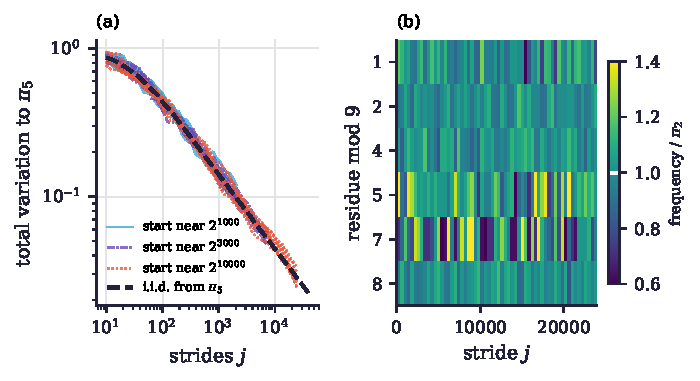
\includegraphics[width=\textwidth]{figures/ch9_orbits.pdf}
\caption{Equidistribution along single orbits. (a) Total variation distance
between the empirical distribution of $y_j\bmod3^5$ along an orbit and the
stationary law $\pi_5$, for $24$ orbits started near $2^{1000}$, $2^{3000}$ and
$2^{10000}$, against the mean distance for independent samples from $\pi_5$
(dashed). (b) Residue frequencies modulo $9$ along one orbit from near
$2^{10000}$, in windows of $400$ strides, relative to $\pi_2$.}
\label{fig:ch9:orbits}
\end{figure}

\section{Three routes and where they fail}\label{sec:ch9:routes}

We end by comparing three routes to the divergence half, each natural, each
developed somewhere in this book, and each failing.

\paragraph{Equidistribution.} If the iterates $y_j$ were equidistributed modulo $2^m$, for every $m$, along every divergent orbit, then $\liminf_N\bar k_N\ge2$ along it by \cref{prop:geom}, which \cref{cor:ch9:freq} forbids; there would be no divergent orbit, and \cref{conj:cesaro} would follow with room to spare.
No such statement can be asked of every orbit, since an orbit that reaches $1$ is eventually constant.
What is known concerns random starting values. Their first halving exponents are close in total variation to independent Geometric$(\tfrac12)$ draws~\cite[Proposition~1.9]{tao2022}, and the deep input of Tao\index{Tao, T.}'s theorem is a fine scale mixing estimate modulo powers of $3$~\cite[Proposition~1.14]{tao2022}.
The theorem establishes a form of equidistribution\index{equidistribution}, but on the $3$ adic side,
in logarithmic density over starting values, and with an exceptional set.
\Cref{lem:ch9:mixing} gives the finite analogue,
exact mixing\index{mixing} of the model chain. Every one of these statements is about an
ensemble or about a Markov chain built from one; the passage from an ensemble
to a single orbit is the step that is missing.

\paragraph{A Lyapunov certificate.} One would like a function $W$ and a constant
$\rho<1$ with $W(S(x))\le\rho W(x)$ for every odd $x\geq3$, which would give
geometric descent with no probabilistic content. \Cref{thm:nolyapunov} rules
this out for every $W$ increasing in $x$, since $S(x)>x$ on the whole class
$x\equiv3\pmod4$, and \cref{cor:ch4:multistride} rules out such $W$ at every fixed number
of strides, since ascents can be chained. A certificate\index{certificate} would have to depend on
the arithmetic of $x$. Certificates of that kind exist if the conjecture holds, for then $W(x)=2^{N(x)}$, where $N(x)$ is the number of strides from $x$ to $1$, satisfies $W(S(x))=\tfrac12W(x)$; but such a certificate, like the total stopping time\index{stopping time} it is built from, presupposes the conjecture. The functions that
do decrease, $\log x$ and $x^p$ for $0<p<1$, decrease in expectation
over a residue class, which is again an ensemble.

\paragraph{Uniform integrability.} Optional stopping for the
martingale\index{martingale} formed by the iterates of the model does not get started: stopped when it first drops to $1$ or below, the martingale is not uniformly integrable\index{uniform integrability} (\cref{prop:uimartingale}), and for the deterministic map the corresponding invariant function, the indicator of reaching $1$, exists trivially, while showing that it equals $1$ everywhere is the conjecture itself (\cref{rem:ch3:cert}). Above all, every martingale here lives on a
probability space of random parities. For a deterministic orbit there is no
filtration with respect to which $\log y_N-N\log\frac34$ is a martingale.

Two of the three failures have the same form: equidistribution and uniform integrability each replace a
statement about a specific trajectory by a statement about a measure, and in
each case the replacement is the step that cannot be justified. A pointwise certificate involves no measure and fails differently: no increasing $W$ works at any fixed number of strides, and the certificates that would work presuppose the answer. The heuristic
is not weak.
Its predictions match the data closely in the tests of this book and of the literature, the total stopping time slope to within about two percent and the variance of the stopping times to about ten percent (\cref{chap:stochastic}).
What is missing is a mechanism that transfers statistics from an ensemble to an
individual orbit, in the presence of a deterministic map that, as far as anyone
knows, has no special structure that would supply one. The Ces\`aro identity
makes the target precise: an orbit that reaches $1$ automatically has
$\bar k_N>\lt$, and an orbit that diverges automatically has
$\limsup\bar k_N\le\lt$. The divergence half of the Collatz conjecture\index{Collatz conjecture} is the
assertion that the second never happens, and the margin of $0.415$ between
the Geometric mean $2$ of the model and the threshold $\lt$ is, so far, a margin that no
argument has been able to transfer to a single orbit.

\section*{Notes}

The observation that a divergent orbit must contain a fraction of odd steps of
at least $1/\lt$ is elementary and has been made many times; it is the
divergence counterpart of the cycle inequality $3^m<2^k$ of \cref{chap:cycles}.
The Ces\`aro identity is the stride formula \eqref{eq:ch2:stride} summed along an orbit, and the pitfall of \cref{rem:ch9:circular} is an immediate consequence of it. The statement that almost every orbit falls below its starting value
is due to Terras\index{Terras, R.}~\cite{terras1976,terras1979} and Everett\index{Everett, C. J.}~\cite{everett1977}; the
exponent $\log3/\log4$ is due to Korec\index{Korec, I.}~\cite{korec1994}. The survey of
Lagarias\index{Lagarias, J. C.}~\cite{lagarias1985} and the volume~\cite{lagarias2010} contain much
more on the $2$ adic picture of \cref{rem:ch9:adic}.

Tao\index{Tao, T.}'s theorem appeared in~\cite{tao2022}; the paper is long but very clearly
written, and its introduction contains an excellent account of the
difficulties described in \cref{sec:ch9:tao}. The
Syracuse random variables and the fine scale mixing\index{mixing} estimate are defined and
proved there, and so are the identities behind the model chain of \cref{sec:ch9:spectral}: the loss of memory~\cite[eq.~(1.21)]{tao2022}, the one step recursion~\cite[Lemma~1.12]{tao2022} and the stationary law~\cite[Remark~1.13]{tao2022}. \Cref{lem:ch9:mixing} restates them in the form of a finite Markov chain. The counting bound
$\pi_1(x)\geq x^{0.84}$ is from Krasikov\index{Krasikov, I.} and Lagarias~\cite{krasikov2003}. The branching random
walk model for the tree of preimages is in Lagarias and Weiss\index{Weiss, A.}~\cite{lagarias1992}.

\begin{sloppypar}
All numerical results in this chapter were computed by the authors with the scripts \texttt{ch9\_spectral.py}, \texttt{ch9\_table.py}, \texttt{ch9\_figures.py}, \texttt{ch9\_numbers.py}, \texttt{ch9\_orbits.py} and \texttt{ch9\_orbits\_check.py} of the code appendix, and the scan of \cref{rem:ch9:circular} with \texttt{ch9\_cesaro\_scan.py}.
\end{sloppypar}

\section*{Exercises}

\begin{exercise}\label{ex:ch9:standard}
State and prove the analogue of \cref{prop:cesaro} for the standard map\index{standard map} $T_0$,
in terms of the number of odd steps among the first $n$ steps. Deduce the
second frequency statement of \cref{cor:ch9:freq} directly.
\end{exercise}

\begin{exercise}\label{ex:ch9:fivex}
For the $5x+1$ map with Syracuse form $y\mapsto(5y+1)/2^{\vt(5y+1)}$, derive
the Ces\`aro identity and show that an orbit that reaches $1$ must have
$\bar k_N>\log_25$. Under the Geometric law the mean exponent is still $2$.
What does this suggest about typical orbits of the $5x+1$ map?
\end{exercise}

\begin{exercise}\label{ex:ch9:mod9}
Compute the matrix $P_2$ of \eqref{eq:ch9:P} on the six units modulo $9$, check
that $P_2^{\,2}$ has identical columns, and verify that they equal
$\tfrac1{63}(8,16,11,4,2,22)$.
\end{exercise}

\begin{exercise}\label{ex:ch9:restricted}
Let $R$ be the operation that deletes from a column stochastic matrix on the
eighteen units modulo $27$ the rows and columns of the nine units with even
representatives in $[0,27)$, and renormalizes the remaining columns. Show that
the limiting nine state matrix of \cref{rem:ch9:oddreps} is $R(P_3)$, that
$R(P_3^{\,3})$ has rank one, and that $R(P_3)^3$ does not. Conclude that the
eigenvalues of the restricted matrix need not reflect the exact mixing\index{mixing} of
\cref{lem:ch9:mixing}.
\end{exercise}

\begin{exercise}\label{ex:ch9:entropy}
Let $q\in(\tfrac12,1)$. Show that the number of binary words of length $n$ with
at least $qn$ ones is $2^{nH(q)+o(n)}$. Using \cref{thm:terras}, deduce that the
proportion of residue classes modulo $2^n$ whose first $n$ accelerated steps
contain at least $n/\lt$ odd steps tends to zero exponentially, and compute
the rate.
\end{exercise}

\begin{exercise}\label{ex:ch9:tao}
Let $K_1,K_2,\ldots$ be independent Geometric$(\tfrac12)$. Compute the law of
$\sum_{m=1}^{3}3^{m-1}2^{-(K_1+\cdots+K_m)}\bmod27$ numerically, and compare it
with the stationary law of $P_3$. Then compute the fine scale discrepancy
$\sum_Y|\pi_3(Y)-\tfrac13\pi_2(Y\bmod9)|$.
\end{exercise}

\chapter{Positive Density from the Backward Tree}\label{chap:backward}

The density theorems of \cref{chap:divergence} fall short in two different ways. The bound of Krasikov and Lagarias (\cref{sec:ch9:krasikov}) counts integers that provably reach $1$, but only about $x^{0.84}$ of those up to $x$, a proportion that tends to zero. Tao's theorem (\cref{sec:ch9:tao}) covers almost every integer, but in logarithmic density and only down to a bound $f(n)$ that must tend to infinity, so it gives no proportion of integers that reach $1$. In September and October 2026 four preprints closed the first of these gaps. Mazur\index{Mazur, L.} proved that for every $t$ not divisible by $3$ the integers whose orbit passes through $t$ have positive lower density, and that a positive proportion of integers reach $1$ within $10.46\log n$ steps of $T_0$~\cite{mazur2026pred,mazur2026time}. Shaik\index{Shaik, I. A.} lowered the constant to any $c>3/\log(4/3)\approx10.428$~\cite{shaik2026}. Lau\index{Lau, K.} gave a quantitative refinement, with a much smaller tower of constants, explicit dependence on the target and step bounds for every target $t$ not divisible by $3$, in a preprint whose mathematics and Lean formalization were produced by the AxiomProver\index{AxiomProver} system~\cite{lau2026}.

This chapter describes what these results say, how the proof is built and what they change for the conjecture, and it tests their numerical side. The proof runs the dynamics backwards: it counts the predecessors of a target in the inverse tree\index{inverse tree}, weighs each by a power of $3$ over a power of $2$, and needs only that residues modulo powers of $3$ mix. The rest of this book runs forwards, along orbits, and the two are dual views of the same random walk, the stride model of \cref{def:ch3:models}. The results are recent and have not been refereed. We have compared the statements quoted here with the texts of the preprints and with Lau's Lean statements, and our own computations agree with every number we report from them, but we have not checked the proofs. Where a consequence is ours rather than the preprints', we say so. \Cref{sec:ch9b:duality} makes precise in what sense the forward model is $2$ adic and the backward model is $3$ adic.

\section{The theorems}\label{sec:ch9b:theorems}

We write $\sigma_0(n)$ for the number of steps of $T_0$ that take $n$ to $1$, the total stopping time of \cref{chap:intro}, and $A(n)$ for the number of odd values among $n,T_0(n),\ldots,T_0^{(\sigma_0(n)-1)}(n)$. For odd $n$, $A(n)$ is the number of steps of the Syracuse map $S$ that take $n$ to $1$. Lau calls the steps of $T_0$ ordinary steps and those of $S$ accelerated steps; the accelerated map $T$ of this book counts neither. Logarithms are natural, and
\[
  D_A=2^{2^{2^{87640}}} .
\]

\begin{theorem}[{Lau~\cite[Theorem~1.3]{lau2026}}]\label{thm:ch9b:lau}
Let $t\ge1$ with $3\nmid t$, and let $X\ge2^{t^3D_A}$. At least $t^{-4}D_A^{-1}X$ odd integers $n<X$ reach $t$ within $10.46\log(n/t)$ steps of $T_0$ and reach the odd part of $t$ within $3.4881\log(n/t)$ steps of $S$.
\end{theorem}

For $t=1$ this is Lau's Corollary~1.2: for every $X\ge2^{D_A}$, at least $X/D_A$ odd integers $n<X$ have $\sigma_0(n)\le10.46\log n$ and $A(n)\le3.4881\log n$. So the integers that reach $1$, and do so in logarithmic time, have positive lower density\index{positive density}. The constants are towers of exponentials and the proportion they guarantee is unimaginably small; \cref{sec:ch9b:steps} shows that the true proportion meeting these step bounds is about one half at every size we can test.

Mazur proved positive density in two manuscripts dated 6 September 2026. The first~\cite[Theorem~1.1]{mazur2026pred} shows that for every $a$ with $3\nmid a$ the set of integers whose orbit under $T_0$ reaches $a$ has positive lower natural density, with a constant depending on $a$, without assuming that $a$ reaches $1$ or that it lies off a cycle. The second~\cite[Theorem~1.1]{mazur2026time} shows that at least $cX$ positive integers $n<X$ have $\sigma_0(n)\le\frac{523}{50}\log n$ once $X\ge X_0$, where $\frac{523}{50}=10.46$ and $c$ and $X_0$ are explicit, given by finite arithmetic expressions~\cite[eq.~(8.6)]{mazur2026time}; Lau's Appendix~B estimates them as $c=D_M^{-1}$ and $X_0=D_M$, with $D_M$ a tower of seven $2$s topped by $173$. Earlier, in July 2026, Mazur had proved the almost bounded theorem of Tao in natural density: for every $f$ tending to infinity, almost every $n$ in natural density has an iterate $T_0^{(k)}(n)<f(n)$ with $k\le C\log n$, for an explicit $C<436$~\cite{mazur2026natural}, as described in~\cite{mazur2026time}. Shaik~\cite{shaik2026}, building on Mazur's construction, obtains positive lower density for convergence within $c\log x$ steps of $T_0$, for the integers below $x$, for every $c>3/\log(4/3)$, with one density bound for all such $c$, and the same range of times for every target not divisible by $3$. Lau's contribution is a quantitative refinement: constants of the size of a tower of height four in place of seven, explicit dependence on the target, step bounds for a general target, which Mazur's first manuscript leaves outside its scope, and a Lean certificate. The condition $3\nmid t$ cannot be dropped: if $3\mid t$, the only predecessor of $t$ under $T_0$ is $2t$, again a multiple of $3$, so the integers whose orbit reaches $t$ are the $2^kt$, a set of density zero (\cref{ex:ch9b:three}).

Lau's preprint and Mazur's two manuscripts were written with substantial help from AI systems, and each says so. Lau's states that AxiomProver autonomously produced the mathematics of the paper and formalized it in Lean, and that the human author is accountable for the statements and conclusions of the introduction and wrote the outline of the argument in its Section~2. Mazur's state that the ProofAtlas.ai harness and OpenAI models contributed substantially to exploration, proof development, formalization and exposition, and that Mazur directed the research and is responsible for the claims; the first adds that it underwent automated reviews, not human peer review, and each comes with a Lean~4 formalization. Lau's Lean files are in a public repository, AxiomMath/CollatzPositiveDensity, written for Lean~4 with the Lean mathematical library. Its challenge file, written by humans, states Corollary~1.2, \cref{thm:ch9b:lau} and Remark~1.4 of the paper with the same constants, step bounds and counts, and we have read those statements; the repository reports that its proofs were checked against them with the Lean comparator, allowing only the standard axioms of propositional extensionality, quotient soundness and choice, and its automatic build succeeds. We have not run the check ourselves. These results join the machine checked work on the sibling problem of Erd\H{o}s~$125$ and our own Lean statements in \cref{sec:ch8:lean}.

The most important consequence for this book is a conditional statement with a three line proof. Mazur states it with upper density~\cite[Corollary~1.2]{mazur2026pred} and Lau with natural density~\cite[Corollary~1.6]{lau2026}; the proof is the same.

\begin{corollary}[{Density one suffices}]\label{cor:ch9b:densityone}
If the set of $n$ whose orbit reaches $1$ has upper natural density one, then every orbit reaches $1$.
\end{corollary}

\begin{proof}
Suppose the orbit of $t$ never reaches $1$. Some point of that orbit is prime to $3$: if $3\mid t$, halve until the value is odd and apply $T_0$ once more, which gives a value $\equiv1\pmod3$. Replace $t$ by that point. Then $t\notin\{1,2,4\}$, and by Mazur's theorem, or by \cref{thm:ch9b:lau}, the integers whose orbit reaches $t$ have positive lower density. None of them reaches $1$: an orbit that met $1$ before $t$ would stay in the cycle $1,4,2$ and never meet $t$, and an orbit that meets $t$ follows the orbit of $t$ from then on. So the integers that do not reach $1$ have positive lower density, and those that do have upper density less than one.
\end{proof}

The following consequences are ours; they are not stated in the preprints, but they follow at once.

\begin{proposition}[A bounded form of Tao's theorem would suffice]\label{prop:ch9b:bounded}
Assume the positive density theorem (\cref{thm:ch9b:lau}, or Mazur~\cite[Theorem~1.1]{mazur2026pred}) and that every integer up to $2^{71}$ reaches $1$~\cite{barina2025}. (a) If the set of $n$ whose orbit reaches $1$ has logarithmic density one, then every orbit reaches $1$. (b) If $\mathrm{Col}_{\min}(n)\le2^{71}$ for all $n$ in a set of logarithmic density one, then every orbit reaches $1$.
\end{proposition}

\begin{proof}
For every set of integers the lower natural density is at most the lower logarithmic density, which is at most the upper logarithmic density, which is at most the upper natural density (\cref{ex:ch9b:densities}). So for (a), logarithmic density one, the density of Tao's theorem, implies upper natural density one, and \cref{cor:ch9b:densityone} applies. For (b), every $n$ in the set reaches an integer at most $2^{71}$, and so reaches $1$. The set of $n$ whose orbit reaches $1$ therefore contains a set of logarithmic density one, so it has logarithmic density one, and (a) applies.
\end{proof}

\Cref{thm:ch1:tao} proves the hypothesis of (b) with $2^{71}$ replaced by any function $f(n)$ that tends to infinity; Mazur's theorem of July 2026 proves it in natural density, again with $f(n)\to\infty$. Tao expected the step from an unbounded $f$ to a bounded one to be almost as hard as the conjecture itself~\cite[Remark~1.4]{tao2022}. If the positive density theorems are right, it is exactly as hard, and the whole problem sits in the gap between a slowly growing $f$ and a constant.

This qualifies a point made twice earlier in the book, that no density statement, however strong, reaches every integer (\cref{sec:ch1:density,sec:ch9:tao}). A density statement about orbits becoming small still does not. A density statement about orbits reaching $1$ now does, through \cref{cor:ch9b:densityone}, because the predecessors of any orbit that missed $1$ would form a set of positive density.

\section{Words, weights and offsets}\label{sec:ch9b:words}

Run the Syracuse map backwards. The odd predecessors of an odd $x$ under $S$ are the integers $(2^ax-1)/3$ with $a\ge1$ and $2^ax\equiv1\pmod3$: an odd $x$ prime to $3$ has infinitely many, and a multiple of $3$ has none. \Cref{sec:ch9:krasikov} describes the same tree for $T_0$.

\begin{definition}[Backward words]\label{def:ch9b:words}
A \emph{word} is a finite sequence $w=(a_1,\ldots,a_d)$ of positive integers, of \emph{length} $|w|=d$ and \emph{degree} $\deg w=a_1+\cdots+a_d$. For odd $n$ put $x_0=n$ and $x_i=(2^{a_i}x_{i-1}-1)/3$ for $1\le i\le d$. The word is \emph{valid at $n$} if every $x_i$ is an integer, and then $\src(w,n)=x_d$ is its \emph{source}. Its \emph{weight} and \emph{offset} are
\[
  \wt(w)=3^d2^{-\deg w},\qquad \off(w)=\sum_{i=1}^{d}3^{i-1}2^{-(a_1+\cdots+a_i)} .
\]
\end{definition}

\begin{proposition}[The offset identity]\label{prop:ch9b:offset}
Let $n$ be odd and $w=(a_1,\ldots,a_d)$ a word. Then $w$ is valid at $n$ if and only if $n\equiv\off(w)\pmod{3^d}$, with $2$ inverted modulo $3^d$. If it is, the $x_i$ are positive odd integers with $\vt(3x_i+1)=a_i$ and $S(x_i)=x_{i-1}$, so that the source reaches $n$ in $d$ steps of $S$ and $d+\deg w$ steps of $T_0$, and
\begin{equation}\label{eq:ch9b:offset}
  n=\wt(w)\,\src(w,n)+\off(w) .
\end{equation}
Weights and offsets compose like the affine maps of \cref{prop:ch2:affine}: $\wt(vw)=\wt(v)\wt(w)$ and $\off(vw)=\off(v)+\wt(v)\off(w)$.
\end{proposition}

\begin{proof}
The composition rules follow from the definitions by splitting the sum for $\off(vw)$ after the letters of $v$. Solving the definition of $x_i$ for $x_{i-1}$ gives $x_{i-1}=(3x_i+1)2^{-a_i}$, and iterating this for the prefix $u=(a_1,\ldots,a_i)$ gives $n=\wt(u)x_i+\off(u)$, whether or not $x_i$ is an integer. Multiplying by $2^{\deg u}$,
\[
  3^ix_i=2^{\deg u}n-N_u,\qquad N_u=2^{\deg u}\off(u)=\sum_{j=1}^{i}3^{j-1}2^{a_{j+1}+\cdots+a_i},
\]
and $N_u$ is an integer, so $x_i$ is an integer if and only if $n\equiv\off(u)\pmod{3^i}$. Since $\off(w)-\off(u)=\wt(u)\off(a_{i+1},\ldots,a_d)$ is divisible by $3^i$ in the $3$ adic integers, the condition for $i=d$ implies it for every $i\le d$. If $x_i$ is an integer, then $2^{a_i}x_{i-1}-1$ is odd, so $x_i$ is odd; $x_i>0$ when $x_{i-1}\ge1$; and $3x_i+1=2^{a_i}x_{i-1}$ with $x_{i-1}$ odd, so $\vt(3x_i+1)=a_i$ and $S(x_i)=x_{i-1}$. The case $i=d$ is \eqref{eq:ch9b:offset}.
\end{proof}

\begin{example}[The word of $11$]\label{ex:ch9b:eleven}
The Syracuse orbit $11\to17\to13\to5\to1$ has letters $a=\vt(3n+1)$ equal to $1,2,3,4$ along the way. Read backward from the target $1$ the word is $w=(4,3,2,1)$: $x_1=(16-1)/3=5$, $x_2=(40-1)/3=13$, $x_3=(52-1)/3=17$, $x_4=(34-1)/3=11$. The word has length $4$ and degree $10$, and $11$ reaches $1$ in $4$ steps of $S$ and $14$ steps of $T_0$. Its weight and offset are $\wt(w)=81/1024$ and $\off(w)=133/1024$, and \eqref{eq:ch9b:offset} reads $1=\frac{81}{1024}\cdot11+\frac{133}{1024}$.
\end{example}

\Cref{eq:ch9b:offset} turns counting predecessors into weighing words. Since $\off(w)>0$, a word valid at $t$ has $\wt(w)<t/\src(w,t)$. Counting sources, rather than words, needs a target that is not on a cycle of $S$.

\begin{lemma}[{Distinct words, distinct sources: Lau~\cite[Lemma~3.3]{lau2026}}]\label{lem:ch9b:distinct}
Let $t$ be an odd positive integer with $S^{(r)}(t)\ne t$ for every $r\ge1$. Then distinct words valid at $t$ have distinct sources.
\end{lemma}

\begin{proof}
Let $w$ be valid at $t$ with source $s$. Read the inverse trajectory forward from $s$: the next value on the forward orbit of $x'$ is $(3x'+1)/2^{a}$, and this is an odd integer only for $a=\vt(3x'+1)$. So $s$ and the length $|w|$ determine $w$, and $S^{(|w|)}(s)=t$. If two lengths $r<r'$ both had $S^{(r)}(s)=S^{(r')}(s)=t$, then $S^{(r'-r)}(t)=t$, which was excluded. So $s$ determines $|w|$, hence $w$.
\end{proof}

So for a target $t$ off the cycles of $S$ and any family of words valid at $t$ whose sources lie in a window $[X,32X)$,
\begin{equation}\label{eq:ch9b:reduction}
  \#\{\text{sources in }[X,32X)\}\;\ge\;\frac{X}{t}\,\beta_X(t),
\end{equation}
where $\beta_X(t)$ is the total weight of the family. A lower bound on $\beta_X(t)$ that does not depend on $X$ is a positive lower density for the predecessors of $t$, and the whole proof is such a lower bound. A target on a cycle is handled through a suitable predecessor off the cycle~\cite{mazur2026pred}.

It is worth seeing what $\beta_X(t)$ is before the proof bounds it from below, and the target $t=1$ is the natural test. It lies on a cycle of $S$, since $S(1)=1$ with the letter $2$, so \cref{lem:ch9b:distinct} does not cover it as it stands: the words $(2)$, $(2,2)$ and so on are all valid at $1$ with the source $1$, and every odd source $s>1$ is the source of the words $(2,\ldots,2,w_s)$ as well as of $w_s$, the word of its Syracuse orbit down to its first visit to $1$. We count each source once, by $w_s$, and write $\beta_X(1)$ for the total weight of these words over the sources in $[X,32X)$; the sources are distinct by construction, so \eqref{eq:ch9b:reduction} holds for this family. Every integer up to $2^{71}$ reaches $1$~\cite{barina2025}, so every odd $n<2^{24}$ is a source, and for $X\le2^{19}$ the window $[X,32X)$ lies below $2^{24}$ and $\beta_X(1)$ is computed from the Syracuse orbit of every odd integer in it. \Cref{tab:ch9b:tree} gives the result, and \cref{fig:ch9b:tree} shows the first levels of the tree.

\begin{figure}[t]
\centering
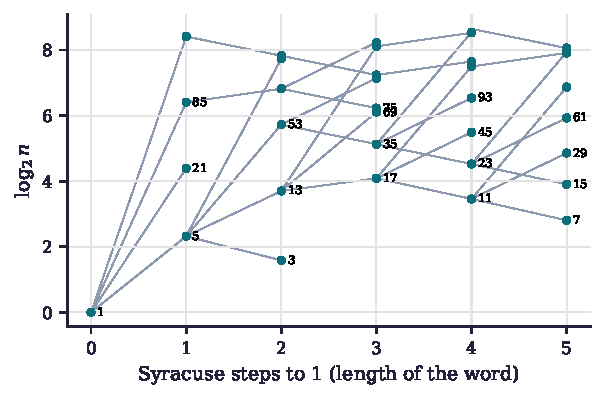
\includegraphics[width=\textwidth]{figures/ch9b_tree.pdf}
\caption{The bottom of the backward tree from $1$: the odd integers below $400$ within five steps of $S$ of $1$, by the length of their word and $\log_2n$. Each edge is one step of $S$; the self loop at $1$, where $S(1)=1$ with the letter $2$, is not drawn.}
\label{fig:ch9b:tree}
\end{figure}

\begin{table}[t]
\centering\footnotesize
\setlength{\tabcolsep}{4pt}
\caption{The backward tree from $1$ below $2^{24}$, exactly. Every odd $n<2^{24}$ reaches $1$, so every odd integer of a window is a source, and each source $s$ is counted once, by the word $w_s$ of its Syracuse orbit down to its first visit to $1$. The second column counts the odd integers in $[X,32X)$, all of them sources; the third counts the sources that a search of the tree truncated at $2^{24}$ finds, and the others have orbits that rise above $2^{24}$ before reaching $1$, so they are lost to the truncation, not to the conjecture. The last column is $31/(2\beta_X(1))$.}
\label{tab:ch9b:tree}
\begin{tabular}{@{}rcccc@{}}
\toprule
$X$ & odd in $[X,32X)$ & found & $\beta_X(1)$ & count$/(X\beta_X)$ \\
\midrule
$2^{4}$ & $248$ & $248$ & $1.5000$ & $10.33$ \\
$2^{6}$ & $992$ & $992$ & $1.4964$ & $10.36$ \\
$2^{8}$ & $3968$ & $3968$ & $1.4918$ & $10.39$ \\
$2^{10}$ & $15\,872$ & $15\,869$ & $1.4889$ & $10.41$ \\
$2^{12}$ & $63\,488$ & $63\,335$ & $1.4892$ & $10.41$ \\
$2^{14}$ & $253\,952$ & $250\,757$ & $1.4897$ & $10.41$ \\
$2^{16}$ & $1\,015\,808$ & $962\,404$ & $1.4892$ & $10.41$ \\
$2^{18}$ & $4\,063\,232$ & $3\,189\,369$ & $1.4891$ & $10.41$ \\
$2^{19}$ & $8\,126\,464$ & $4\,720\,635$ & $1.4891$ & $10.41$ \\
\bottomrule
\end{tabular}
\end{table}

Three things are visible in \cref{tab:ch9b:tree}. First, the total weight is nearly the same in every window, but not exactly: $\beta_X(1)$ falls from $1.5000$ at $X=2^4$ to $1.4889$ at $2^{10}$, and then stays between $1.4889$ and $1.4897$ up to $2^{19}$. The harmonic sum does not explain the value: over the odd $s$ in a window of ratio $32$, $\sum1/s=\frac12\log32+O(X^{-2})\approx1.733$, not $1.49$. For the target $1$, \eqref{eq:ch9b:offset} gives $\wt(w_s)\,s=1-\off(w_s)<1$ for every source, and by \cref{prop:ch9b:steps} this is $3^{A(s)}s/2^{H(s)}=2^{-\varepsilon(s)}$, so that
\[
  \beta_X(1)=\sum_{s}\frac{2^{-\varepsilon(s)}}{s},
\]
the sum over the odd $s$ in $[X,32X)$. The mean of $2^{-\varepsilon(s)}$ over the window, weighted by $1/s$, is $\beta_X(1)/\bigl(\frac12\log32\bigr)$, between $0.859$ and $0.866$ in every row. It is set mostly by the last few odd values of the orbit before $1$, where $1/(3m_i)$ is not small, and its stability from window to window is the empirical fact that the table shows. Second, the reduction \eqref{eq:ch9b:reduction} loses the factor in the last column, $31/(2\beta_X(1))\approx10.41$. It splits as $31/\log32\approx8.94$, from replacing $1/s$ by $1/X$ across a window of ratio $32$, times $\frac12\log32/\beta_X(1)\approx1.16$, the gap between $\wt(w_s)$ and $1/s$ averaged over the window: most of the loss is the window, not the offset. Third, the proof of \cref{thm:ch9b:lau} does not bound this quantity but the weight of its own family of words, which pass through a seed (\cref{sec:ch9b:generations}): for $X$ past the threshold of the theorem, $\beta_X(t)\ge2^{-160071}t^{-1.34}$ (Lau's Proposition~7.2), against the $1.49$ of the table. The longest word below $2^{24}$ has $263$ letters, at $n=15\,733\,191$.

\section{The forward model is \texorpdfstring{$2$}{2} adic, the backward model is \texorpdfstring{$3$}{3} adic}\label{sec:ch9b:duality}

We make precise the remark with which the chapter opened, that the forward and the backward walk are dual, because it is the bridge between this chapter and the rest of the book.

Fix a word $w=(a_1,\ldots,a_d)$ with $\deg w=D$. Which odd integers $n$ have $w$ as the first $d$ letters of their forward Syracuse orbit, that is, $\vt(3S^{(i-1)}(n)+1)=a_i$ for $1\le i\le d$? They form one residue class modulo $2^{D+1}$. This is \cref{thm:terras} read through \cref{prop:geom}: the word $w$ is the parity vector $1\,0^{a_1-1}\cdots1\,0^{a_d-1}\,1$ of $T$, of length $D+1$. Among the odd integers the class has density $2^{-D}=\prod_i2^{-a_i}$, so that under Haar measure on the odd $2$ adic integers the forward letters are independent and geometric with mean two (\cref{sec:ch2:adic}).

Now ask the backward question. By \cref{prop:ch9b:offset}, the odd targets $n$ at which $w$ is valid form the single class $n\equiv\off(w)\pmod{3^d}$, of density $3^{-d}$ among the odd integers. So $\wt(w)=3^d2^{-D}$ is the ratio of the two densities, forward over backward, and by \eqref{eq:ch9b:offset} going backward along $w$ divides $n$ by this ratio, up to the offset. In the stride model of \cref{def:ch3:models} a stride changes $\log x$ by $\log3-K\log2$, and $\log\wt(w)=\sum_i(\log3-a_i\log2)$ is a sum of the same increments, so the forward walk of $\log x$ and the backward walk of $\log\wt$ are one random walk run in two directions.

So where is the difficulty? In each direction one of the two sets is exact and the other has to be averaged. Forward, one fixes the word and the set of $n$ is a residue class; that is why Terras could show that almost every $n$ eventually drops below itself. The trouble is iteration. Under Haar measure the residues of $T^{(k)}(x)$ stay uniform at every step (\cref{prop:ch2:haar}), but for integers the parities of the orbit of $n$ are exact only for about $\log_2n$ steps of $T$, roughly a fifth of a typical orbit (\cref{prop:ch3:exact}), and after that the forward walk is a model. Backward, one fixes the target and asks for the total weight of valid words, the residue density $\rho_d(n)$ of \cref{sec:ch9b:density}. Its average over all residues is exactly one, and over the units it is $\frac32$ (\cref{ex:ch9b:units}), but at a particular $n$ it can be large or small (\cref{sec:ch9b:offsets}). Tao's theorem is itself a forward theorem, about the iterates $S^{(m)}(N)\bmod3^m$ (\cref{sec:ch9:tao}), and it reaches the $3$ adic side because reversing the order of the exponents in the affine formula for those iterates turns it into an offset (\cref{sec:ch9b:density}). On that side the offsets mix modulo powers of $3$, and the rate of mixing is bounded by Fourier analysis on $\Z/3^d\Z$ (\cref{sec:ch9b:mixing}).

The open problem O1 (Problem~\ref{prob:ch11:o1}), equidistribution, and the parity autocorrelations of \cref{sec:ch3:autocorr} are the forward names for this obstruction. \Cref{sec:ch9b:offsets} measures its backward form directly.

\section{The residue density}\label{sec:ch9b:density}

Let $W=(a_1,a_2,\ldots)$ have independent letters with $\Prob(a_i=k)=2^{-k}$ for $k\ge1$, the law of the halving exponents $K_j$ in the stride model of \cref{def:ch3:models}. Then $\E a_i=2$, and $\log\wt(W_{\le d})=d\log3-\deg(W_{\le d})\log2$ is a random walk with drift $\log3-2\log2=\log\frac34$ per letter: the drift of the stride model, read backwards. A fixed word $w$ of length $d$ is the prefix $W_{\le d}$ with probability $2^{-\deg w}$, so
\[
  \wt(w)=3^d\,\Prob(W_{\le d}=w) .
\]
Let $\pi_d$ be the law of $\off(W_{\le d})$ modulo $3^d$. Reversing the order of the exponents in the affine formula for $S^{(m)}(N)\bmod3^m$ of \cref{sec:ch9:tao} turns it into an offset, and the letters are independent and identically distributed, so $\pi_d$ is the law of Tao's Syracuse random variable\index{Syracuse random variable}, the law $\pi_d$ of \cref{lem:ch9:mixing}. Write $\rho_d=3^d\pi_d$ for its density with respect to the uniform law on $\Z/3^d\Z$.

\begin{proposition}[Total weight is a residue density]\label{prop:ch9b:density}
For odd $n$ and $d\ge1$,
\[
  \sum_{|w|=d}\wt(w)\,\mathbf 1[w\text{ valid at }n]=\rho_d(n\bmod3^d) .
\]
\end{proposition}

\begin{proof}
By \cref{prop:ch9b:offset} the sum is $3^d\,\Prob\bigl(\off(W_{\le d})\equiv n\pmod{3^d}\bigr)=3^d\pi_d(n\bmod3^d)$.
\end{proof}

So the total weight of the backward words of length $d$ from $n$ is the density of $\pi_d$ at $n$, and the arithmetic of the problem lives in $\pi_d$. Since $\off(w)\equiv2^{-a_1}\pmod3$, the law $\pi_d$ lives on the units modulo $3^d$, where $\rho_d$ averages $\frac32$, and it charges every unit (\cref{ex:ch9b:units}). The density is far from constant at coarse scales, as \cref{sec:ch9b:offsets} shows, and what the proof needs is Tao's statement that it is nearly constant at fine scales relative to coarse ones.

\begin{example}[The densities $\rho_1$ and $\rho_2$]\label{ex:ch9b:rhotwo}
At level one, $\off(W_{\le1})\equiv2^{-a_1}\pmod3$ is $1$ when $a_1$ is even and $2$ when $a_1$ is odd, so $\rho_1=(0,1,2)$ on the residues $0,1,2$: a target congruent to $2$ modulo $3$ carries twice the weight of one congruent to $1$, which is the familiar fact that $n\equiv5\pmod6$ has predecessors under $S$ for odd $a$ and $n\equiv1\pmod6$ for even $a$. At level two the order of $2$ modulo $9$ is six, and summing the geometric series over the residues of $a_1$ modulo six and of $a_2$ modulo two gives
\[
  \rho_2=\Bigl(\tfrac87,\ \tfrac{16}7,\ \tfrac{11}7,\ \tfrac47,\ \tfrac27,\ \tfrac{22}7\Bigr)\quad\text{on the units }1,2,4,5,7,8\ \text{of }\Z/9\Z .
\]
The average over the six units is $\tfrac32$, as it must be, and the spread is already a factor of eleven. Targets congruent to $8$ modulo $9$ carry a large total weight of words of length $2$ and targets congruent to $7$ carry little.
\end{example}

\section{Fine scale mixing with explicit constants}\label{sec:ch9b:mixing}

Tao proves that the Fourier coefficients of $\pi_n$ at frequencies prime to $3$ decay faster than any power of $n$~\cite[Proposition~1.17]{tao2022}, and deduces the fine scale mixing\index{mixing} of \cref{sec:ch9:tao}. Lau proves explicit forms of both estimates, the first in Sections~9 to~14 of~\cite{lau2026} and the second in its Section~4. We state them without proof; $\widehat\pi_n(\xi)=\sum_y\pi_n(y)e^{-2\pi i\xi y/3^n}$ and $D_*$ is an explicit constant.

\begin{proposition}[{Fourier bound and fine scale mixing, Lau~\cite[Theorem~14.6 and Proposition~4.1]{lau2026}}]\label{prop:ch9b:mixing}
For every $n\ge1$ and every $\xi$ prime to $3$,
\[
  |\widehat\pi_n(\xi)|\le(160D_*)^{A_*}n^{-A_*},\qquad A_*=\tfrac{10241}{4096}.
\]
Consequently, for $2^{80000}\le m\le d$,
\begin{equation}\label{eq:ch9b:mixing}
  3^{-d}\sum_{y\bmod3^d}\bigl|\rho_d(y)-\rho_m(y\bmod3^m)\bigr|\le Cm^{-3/2},
\end{equation}
with $\log_2C\approx87532.002$.
\end{proposition}

The proof of the Fourier bound pairs consecutive letters and locates the \emph{black points}, where the character sum shows no cancellation; under the map $(j,l)\mapsto3^{2(j-1)}2^{1-l}\xi$ they form disjoint triangles, and a renewal process on the sums $a_{2i-1}+a_{2i}$ of paired letters, split after each pair whose sum is $4$ or $5$, controls how long a path can stay among them. Cutting a random word at the first time its degree passes $n\lt$, less a logarithmic correction, and convolving the head with the transported law of the tail converts the Fourier bound into fine scale mixing. In the notation of \cref{sec:ch9:tao} the left side of \eqref{eq:ch9b:mixing} is $\sum_Y|\pi_d(Y)-3^{m-d}\pi_m(Y\bmod3^m)|$, the quantity of Tao's Proposition~1.14, here with the exponent $\frac32$ and an explicit constant. The exponent is $A_*-\alpha/2$, where $\alpha=\frac{4097}{2048}$ is the growth exponent of a bound $8m^\alpha$ for a bounded part of $\rho_m$; a bounded part is needed because $\rho_m$ itself is unbounded (\cref{sec:ch9b:offsets}).

The towers in \cref{thm:ch9b:lau} come from the size of these constants. The generations of the next section must start where the summed propagation errors are smaller than the mass they carry, and with $\log_2C\approx87532$ that is generation $j_0=6103914$. The residue level there is $d_0=2^{87639}$, a seed for a general target can need about $4\cdot3^{d_0}$ binary digits more than the target, and $\log_2D_A=4^{d_0}$.

\section{Generations and the census}\label{sec:ch9b:generations}

Words are grown in blocks. In the plane of length and degree a word traces a lattice path, and its weight $3^d2^{-\deg w}$ is constant along lines of slope $\lt$. Block $j$ is cut at the first crossing of the line of slope $\lt$ through $(\delta_j,2\delta_j)$, with scales $\delta_j\approx200\cdot1.01^j$ and overshoot caps $R_j=16+\lfloor j/32\rfloor$. A family of first crossings is prefix free, so its weights behave like the probabilities of a stopping time and optional stopping applies to them.

For a scale $\delta$ and a cap $R$, the first crossing family $\mathrm{FC}(\delta,R)$ is built as follows. A random word has degree about twice its length, so its path typically crosses the line of slope $\lt$ through $(\delta,2\delta)$ near $(\delta,2\delta)$. Cut each word at its first crossing, and keep those whose length lies within $\lfloor3\delta/5\rfloor$ of $\delta$ and whose overshoot above the line is at most $R$. The family is finite, and its mass $\sum_{w\in\mathrm{FC}(\delta,R)}2^{-\deg w}$ is the probability that the stopped walk lands in the allowed set, which Chernoff bounds show is close to one (Lau's Section~15); the construction is Mazur's, with Lau's constants. \Cref{fig:ch9b:crossing} shows twelve random words and their first crossings at $\delta=40$; two of them cross only after length $64$, outside the window, and the family discards them.

\begin{figure}[t]
\centering
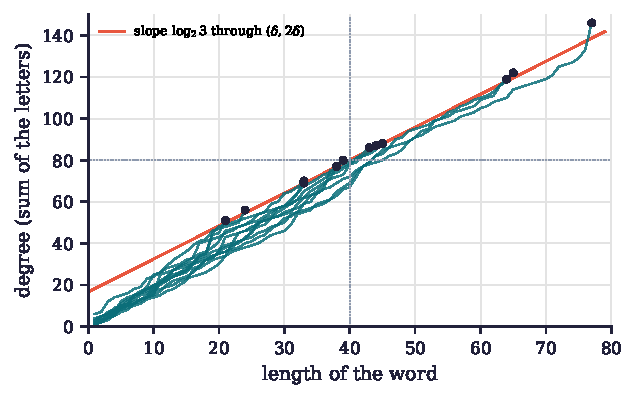
\includegraphics[width=\textwidth]{figures/ch9b_crossing.pdf}
\caption{First crossings at scale $\delta=40$ for twelve random words (of fourteen drawn, two do not cross within $80$ letters). Each path is the degree of a random word against its length; the dot marks the first crossing, after length $2\delta/5=16$, of the line of slope $\lt$ through $(\delta,2\delta)$, on which the weight $3^d2^{-\deg w}$ equals $(3/4)^\delta$, and the word is cut there.}
\label{fig:ch9b:crossing}
\end{figure}

A word in $\mathrm{FC}(\delta,R)$ of length $|w|$ and degree $\deg w=|w|\lt+(2-\lt)\delta+o$, where $0\le o\le R$ is its overshoot, has
\[
  \wt(w)=3^{|w|}2^{-\deg w}=(3/4)^{\delta}\,2^{-o},
\]
independent of its length. So by \eqref{eq:ch9b:offset} each block multiplies the source by about $(4/3)^{\delta}2^{o}$, whatever the length of the block, and the weights of all words built from the same sequence of blocks lie within a factor $2^{R_1+\cdots+R_j}$ of one another.

The \emph{weighted density}
\[
  Z_j(t)=\sum_{w\in L_j}\wt(w)\,\rho_{\lfloor\delta_j/4\rfloor}(s_w),
\]
where $L_j$ is the family of words of generation $j$ valid at $t$ and $s_w$ the source of $w$, weighs each word by the residue density of its source, that is, by the total weight of the words that can continue it (\cref{prop:ch9b:density}). Before the restriction to words valid at $t$, the words of generation $j$ form the family $\bar L_j$ of concatenations of $j$ first crossing blocks, where for $j\ge5$ the first five blocks must pass Lau's five block selector, a set of bounds on their rounded offsets that keeps the offset of every selected word between $85/256$ and $637/256$; its mass is $\mathrm{mass}(\bar L_j)=\sum_{w\in\bar L_j}2^{-\deg w}$. Fine scale mixing (\cref{prop:ch9b:mixing}) gives the propagation bound, which is summable.

\begin{proposition}[{Propagation, Lau~\cite[Proposition~6.1]{lau2026}, making explicit Mazur~\cite[Proposition~3.1]{mazur2026time}}]\label{prop:ch9b:propagation}
For every $j\ge6\times10^6$,
\[
  |Z_{j+1}(t)-Z_j(t)|\le Fj^{5/2}\,1.01^{-j},\qquad F=\tfrac92(C+1),\quad\log_2F<87534.2,
\]
with $C$ the constant of \eqref{eq:ch9b:mixing}.
\end{proposition}

From $j_0=6103914$ on, the remaining errors are small: they sum to less than $\frac54\cdot2^{-24}$, so that $Z_j(t)>2^{-25}$ for every $j\ge j_0$ wherever $Z_{j_0}(t)>2^{-23}$. At $j_0$ the function $Z_{j_0}$ is periodic modulo $3^{2^{87639}}$ and averages $\frac32\,\mathrm{mass}(\bar L_{j_0})>2^{-23}$ over the units, so some residue class $y_0$ has $Z_{j_0}>2^{-23}$. A seed $t_1=(2^at-1)/3$ in the class $y_0$ starts the construction from a general target, a terminal block places the sources in $[X,32X)$, and a census inequality, using the bound $8m^\alpha$ for the bounded part of the density, turns a terminal weighted density of at least $2^{-26}$ into $\beta_X(t)\ge2^{-160071}t^{-1.34}$; this is about where the exponent $160071$ comes from, since $2^{-26}/(8m^\alpha)\approx2^{-160068}$ at $m=2^{80000}$. Two small facts make the seed available: part (1) below is Lau's lemma on candidate residues, and part (2), with the use of two candidates, is from his Section~7.

\begin{lemma}[{Candidate seeds, after Lau~\cite{lau2026}}]\label{lem:ch9b:seed}
Let $3\nmid t$ and let $a_\circ\in\{38,39\}$ have $2^{a_\circ}t\equiv1\pmod3$. (1) For every $q\ge1$ and $i_0\ge0$, the integers $(4^{i}\,2^{a_\circ}t-1)/3$ for $i_0\le i<i_0+3^{q}$ meet every residue class modulo $3^{q}$ exactly once. (2) If two odd integers $y\ne y'$ satisfy $S(y)=S(y')$, at most one of them lies on a cycle of $S$.
\end{lemma}

\begin{proof}
For (1), the numbers are integers since $4^i2^{a_\circ}t\equiv2^{a_\circ}t\equiv1\pmod3$. The difference of the integers at $i<i'$ is $4^{i}2^{a_\circ}t\,(4^{e}-1)/3$ with $e=i'-i$, and $\nu_3(4^{e}-1)=1+\nu_3(e)$, which one checks by induction on $\nu_3(e)$. If $3\nmid e$, then $4^e-1=3(1+4+\cdots+4^{e-1})$ and the second factor is $\equiv e\not\equiv0\pmod3$, since $4\equiv1\pmod3$. If $3\mid e$, put $x=4^{e/3}\equiv1\pmod3$; then $4^e-1=(x-1)(x^2+x+1)$ and $x^2+x+1\equiv3\pmod9$, so $\nu_3(4^e-1)=\nu_3(4^{e/3}-1)+1$. Since $3\nmid t$ and $e<3^q$, the difference has $3$ adic order $\nu_3(e)<q$, and the $3^{q}$ integers are pairwise incongruent. For (2), if $S^{(j)}(y)=y$ and $S^{(j')}(y')=y'$ then with $r=jj'$ both are fixed by $S^{(r)}$, and $y=S^{(r-1)}(S(y))=S^{(r-1)}(S(y'))=y'$.
\end{proof}

Lau takes two candidates $t_1=(2^at-1)/3$ with $a=a_\circ+2i$ in the class $y_0$ modulo $3^{d_0}$, one with $i<3^{d_0}$ and one with $3^{d_0}\le i<2\cdot3^{d_0}$; by (1) each range contains exactly one. Both map to the odd part of $t$ in one step of $S$, so by (2) at least one is off every cycle, and \cref{lem:ch9b:distinct} applies to it. This is the only place cycles enter the argument, and they enter only to be avoided.

Read through \cref{chap:stochastic}, the propagation bound says that $Z_j$ is conserved from one generation to the next up to summable errors, as the expectation of a martingale is conserved under optional stopping. This is where the backward argument meets the martingale methods of this book.

\section{The two step constants are one constant}\label{sec:ch9b:constants}

\begin{proposition}[Steps of $T_0$ and steps of $S$]\label{prop:ch9b:steps}
Let the orbit of $n$ under $T_0$ reach $1$, let $m_1,\ldots,m_{A(n)}$ be its odd values before $1$, and let $H(n)=\sigma_0(n)-A(n)$ be its number of halvings. Then $2^{H(n)}=n\,3^{A(n)}\prod_i\bigl(1+\frac1{3m_i}\bigr)$, so that
\begin{equation}\label{eq:ch9b:steps}
  \sigma_0(n)=(1+\lt)A(n)+\log_2n+\varepsilon(n),\qquad \varepsilon(n)=\sum_{i=1}^{A(n)}\log_2\Bigl(1+\frac1{3m_i}\Bigr)\ge0 .
\end{equation}
\end{proposition}

\begin{proof}
An odd step multiplies the current value $m$ by $3(1+\frac1{3m})$ and a halving divides it by $2$, and the product of all these factors takes $n$ to $1$. Take logarithms to base $2$ and add $A(n)$.
\end{proof}

A bound $A(n)\le c\log n$ therefore gives $\sigma_0(n)\le\bigl((1+\lt)c+1/\log2\bigr)\log n+\varepsilon(n)$, and
\[
  (1+\lt)\cdot3.4881+\frac1{\log2}=10.4593<10.46 .
\]
This is how the two constants of \cref{thm:ch9b:lau} are tied: the bound for steps of $T_0$ follows from the bound for steps of $S$ in this way, with $\varepsilon$ absorbed by replacing $\log3$ with $\log(3+\frac1{4096})$, which is Mazur's condition $c_{\mathrm{acc}}\bigl(\log2+\log(3+\frac1{4096})\bigr)+1\le\frac{523}{50}\log2$ for a constant $c_{\mathrm{acc}}$ of accelerated steps. At the level of the model the same identity reads
\[
  \frac{1+\lt}{\log(4/3)}+\frac1{\log2}=\frac3{\log(4/3)},
\]
which is equivalent to $\log\frac43=(2-\lt)\log2$. So $3/\log(4/3)\approx10.428$ and $1/\log(4/3)\approx3.476$ are the drift constants of the stride model, $\log\frac34$ per stride and $\frac13\log\frac34$ per step of $T_0$, read backwards: a stride is on average $1+\E K=3$ steps of $T_0$. For the accelerated map, whose steps each contain one halving, the same count gives the slope $2/\log(4/3)=\gamma_0\approx6.952$ of \cref{chap:stochastic}.

\section{Step counts below \texorpdfstring{$3\cdot10^6$}{3 million}}\label{sec:ch9b:steps}

\Cref{tab:ch9b:steps} and \cref{fig:ch9b:steps} give $\sigma_0(n)$ and $A(n)$ for every $n$ with $10^4\le n<3\cdot10^6$, even and odd. Two points stand out. The share of $n$ meeting both of Lau's bounds is about $0.54$, against the proven $D_A^{-1}$: the tower is an artefact of the proof, not of the phenomenon. And the two bounds hold for exactly the same $n$ in every range. By \eqref{eq:ch9b:steps} the conditions $\sigma_0(n)\le10.46\log n$ and $A(n)\le3.4881\log n$ differ only when $A(n)$ lies between $3.4881\log n$ and $3.48837\log n-0.387\,\varepsilon(n)$, an interval of length $|0.0003\log n-0.387\,\varepsilon(n)|$, and no $n$ in the table has $A(n)$ there.

\begin{table}[t]
\centering\footnotesize
\caption{Steps of $T_0$ and of $S$ for $10^4\le n<3\cdot10^6$: the mean and standard deviation of $\sigma_0(n)/\log n$, the renewal prediction $16.42/\sqrt{\log n}$ for the standard deviation at the midpoint of the range, the mean of $A(n)/\log n$, and the share of $n$ meeting both of Lau's bounds $\sigma_0(n)\le\lfloor10.46\log n\rfloor$ and $A(n)\le\lfloor3.4881\log n\rfloor$. In every range the two bounds hold for exactly the same $n$.}
\label{tab:ch9b:steps}
\begin{tabular}{@{}lccccc@{}}
\toprule
range of $n$ & mean $\sigma_0/\log n$ & sd & predicted sd & mean $A/\log n$ & share \\
\midrule
$[10^4,10^5)$ & $10.219$ & $4.73$ & $4.97$ & $3.387$ & $0.552$ \\
$[10^5,10^6)$ & $10.258$ & $4.31$ & $4.52$ & $3.404$ & $0.541$ \\
$[10^6,3\cdot10^6)$ & $10.264$ & $4.11$ & $4.31$ & $3.407$ & $0.539$ \\
\bottomrule
\end{tabular}
\end{table}

\begin{figure}[t]
\centering
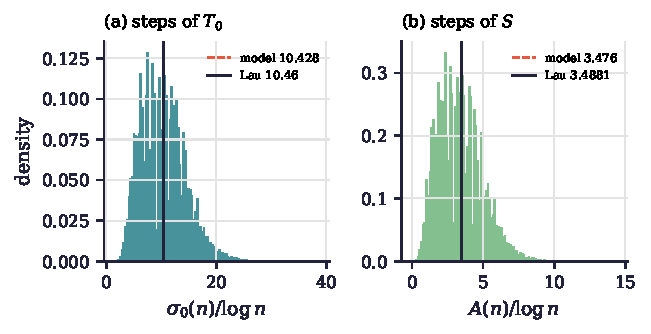
\includegraphics[width=\textwidth]{figures/ch9b_steps.pdf}
\caption{Steps to reach $1$ for $10^6\le n<3\cdot10^6$. (a) Histogram of $\sigma_0(n)/\log n$, with the model constant $3/\log(4/3)\approx10.428$ (dashed) and Lau's $10.46$ (solid). (b) Histogram of $A(n)/\log n$, with $1/\log(4/3)\approx3.476$ and Lau's $3.4881$. The comb comes from dividing integers by $\log n$ over a narrow range of $n$.}
\label{fig:ch9b:steps}
\end{figure}

The spread is the renewal\index{renewal} central limit theorem of \cref{sec:ch3:clt}. In the stride model a stride changes $\log x$ by $\log3-K\log2$, up to the plus one of \cref{rem:ch3:plusone}, with mean $\log\frac34$ and variance $2(\log2)^2$, since $K$ has variance $2$. The number of strides $A(n)$ is the first passage time below $0$ from $\log n$, and \eqref{eq:ch3:clt} gives
\[
  \frac{A(n)}{\log n}\approx\frac1{\log(4/3)}+\frac{\sqrt2\log2}{(\log\frac43)^{3/2}}\,\frac{Z}{\sqrt{\log n}},\qquad \frac{\sqrt2\log2}{(\log\frac43)^{3/2}}=6.353,
\]
with $Z$ standard normal. By \eqref{eq:ch9b:steps}, $\sigma_0$ inherits the factor $1+\lt$, so the standard deviation of $\sigma_0(n)/\log n$ is about $16.42/\sqrt{\log n}$. For the accelerated map the same identity reads $\sigma_\infty(n)=\lt A(n)+\log_2n+\varepsilon(n)$, and it turns the variance of the stride model into $(\lt)^2\cdot6.353^2\log n\approx101.4\log n$, the variance that \cref{sec:ch3:clt} computes from the coin model of $T$: the two models agree, as they must. The prediction in \cref{tab:ch9b:steps} is about five percent high throughout, consistent with the orbits being slightly less dispersed than the independent model at these sizes.

The consequence for Lau's constant is stark. The margin above the limiting mean is $10.46-3/\log(4/3)=0.0318$, so the share of $n$ meeting the bound $10.46\log n$ is roughly $\Phi\bigl(0.0318\sqrt{\log n}/16.42\bigr)$, which differs from one half by less than one percent for every $n$ below $10^{12}$, where a census is possible. The excess over one half in \cref{tab:ch9b:steps} comes from finite size: at these sizes the mean of $\sigma_0(n)/\log n$ is about $10.26$, below its limit, and the law is skewed to the right. Ninety percent coverage needs $\log n\approx4.4\times10^5$, an $n$ of about $190\,000$ digits, and ninety nine percent about $626\,000$ digits. Shaik's threshold is therefore the natural endpoint: for $c<3/\log(4/3)$ the same calculation sends the share to zero, which is the heuristic content of Problem~\ref{prob:ch11:b3}.

\section{The offset law in exact arithmetic}\label{sec:ch9b:offsets}

The mixing input can be tested directly. The offset of a word satisfies $\off(a\,v)=2^{-a}\bigl(1+3\off(v)\bigr)$, and $3\off(v)$ modulo $3^d$ depends only on $\off(v)$ modulo $3^{d-1}$, so $\pi_d$ is obtained from $\pi_{d-1}$ exactly:
\[
  \pi_d(z)=\sum_{a\ge1}2^{-a}\sum_{y:\ 2^{-a}(1+3y)\equiv z}\pi_{d-1}(y) .
\]
We evaluate this with the letters truncated at $a\le60$ and renormalized, which moves $\pi_d$ by at most $d\,2^{-60}$ in total variation, for $d\le18$, where $3^{18}\approx3.9\times10^8$, with a full Fourier transform at every level. \Cref{tab:ch9b:offsets} and \cref{fig:ch9b:fourier} report the largest Fourier coefficient at frequencies prime to $3$, the frequency attaining it, and the mean distances of $\rho_d$ from the lifts of $\rho_{d-1}$ and $\rho_{\lceil d/2\rceil}$. Four things stand out.

\begin{table}[t]
\centering\footnotesize
\setlength{\tabcolsep}{4pt}
\caption{The exact $3$ adic offset law. For each level $d$: the largest Fourier coefficient of $\pi_d$ at frequencies prime to $3$, the frequency in $[1,3^d/2]$ attaining it, that coefficient times $d^2$, the mean distance $3^{-d}\sum_y|\rho_d(y)-\rho_m(y\bmod3^m)|$ for $m=d-1$ and for $m=\lceil d/2\rceil$, and the largest value of $\rho_d$.}
\label{tab:ch9b:offsets}
\begin{tabular}{@{}rcccccc@{}}
\toprule
$d$ & $\max_{3\nmid\xi}|\widehat\pi_d(\xi)|$ & worst $\xi$ & $d^2\max|\widehat\pi_d|$ & $m=d-1$ & $m=\lceil d/2\rceil$ & $\max\rho_d$ \\
\midrule
$4$ & $0.1770$ & $2^{4}$ & $2.83$ & $0.343$ & $0.535$ & $7.27$ \\
$8$ & $0.0609$ & $2^{9}$ & $3.90$ & $0.213$ & $0.459$ & $37.3$ \\
$10$ & $0.0383$ & $2^{12}$ & $3.83$ & $0.178$ & $0.436$ & $84.2$ \\
$12$ & $0.0265$ & $2^{14}$ & $3.81$ & $0.151$ & $0.414$ & $189.6$ \\
$14$ & $0.0191$ & $2^{17}$ & $3.75$ & $0.130$ & $0.393$ & $426.8$ \\
$16$ & $0.0144$ & $2^{20}$ & $3.69$ & $0.112$ & $0.373$ & $960.3$ \\
$17$ & $0.0125$ & $2^{21}$ & $3.62$ & $0.104$ & $0.345$ & $1440.6$ \\
$18$ & $0.0112$ & $2^{23}$ & $3.62$ & $0.097$ & $0.354$ & $2160.9$ \\
\bottomrule
\end{tabular}
\end{table}

\begin{figure}[t]
\centering
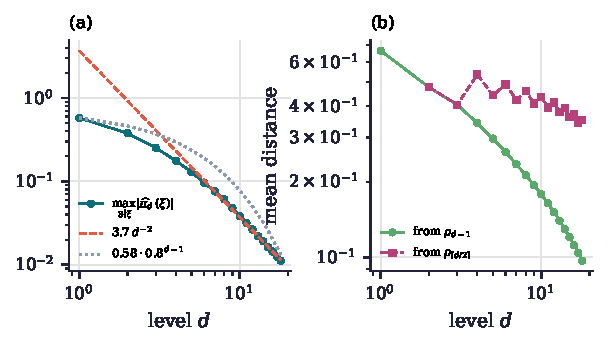
\includegraphics[width=\textwidth]{figures/ch9b_fourier.pdf}
\caption{The exact offset law, levels $1$ to $18$. (a) The largest Fourier coefficient of $\pi_d$ at frequencies prime to $3$, against $3.7\,d^{-2}$ (dashed) and the geometric curve $0.58\cdot0.8^{d-1}$ (dotted). (b) The mean distance of $\rho_d$ from the lift of $\rho_{d-1}$ and from the lift of $\rho_{\lceil d/2\rceil}$.}
\label{fig:ch9b:fourier}
\end{figure}

\begin{enumerate}
\item The decay is not geometric over this range. The ratio of consecutive maxima climbs from $0.65$, between levels $1$ and $2$, to $0.89$, between levels $17$ and $18$, while $d^2\max_\xi|\widehat\pi_d(\xi)|$ is nearly flat, drifting from $3.9$ at $d=8$ to $3.6$ at $d=18$ (it stays between $3.62$ and $3.90$ for $7\le d\le18$). Locally the decay looks like a power of $d$ near $2$, slowly steepening. This is consistent with Tao's theorem, which gives decay faster than any power asymptotically, but it says that the preasymptotic regime is long.
\item The worst frequency is a power of $2$. Since $2$ generates the units modulo $3^d$, every frequency prime to $3$ is a power of $2$ modulo $3^d$; the point is that the maximizing frequency, taken in $[1,3^d/2]$, is a power of $2$ as an integer, at every level $d\le18$, with every frequency prime to $3$ scanned: $2^k$ with $d\le k\le1.28\,d$ for $2\le d\le18$ ($k/d=1.278$ at $d=18$, where $k=23$). \Cref{tab:ch9b:profile} shows the profile of $|\widehat\pi_d(2^k)|$ over $k$ for $d=14$ to $18$: a smooth bump in $k$, about six values of $k$ wide at half its height, whose peak moves right by one or two per level. Multiplication by $2$ is the symmetry generated by the letters, and a plausible reason is that a frequency $2^k$ sees the first letter through the small integer $2^{k-a_1}$, where the cancellation is weakest. Any sharp bound will have to treat this orbit of frequencies separately, much as Lau's black triangles do.
\item The residue density is far from bounded: $\max\rho_d$ grows by a factor $\frac32$ per level (between $1.50004$ and $1.50014$ at levels $15$ to $18$), like the weight $(3/2)^d$ of the word of $d$ ones (\cref{ex:ch9b:ones}). This is why the census uses a bounded part of the density in place of $\rho_m$ itself.
\item Mixing across levels is slow. The distance from the lift of $\rho_{d-1}$ falls only like $d^{-0.84}$ over $4\le d\le18$ ($d^{-0.97}$ over $8\le d\le18$), and the distance from the lift of $\rho_{\lceil d/2\rceil}$ is still $0.35$ at $d=18$. A bound of the form $Cm^{-3/2}$ with $m=\lceil d/2\rceil$, as in \eqref{eq:ch9b:mixing}, holds at these levels only with $C\ge9.5$, and the constant needed rises steadily ($8.45$ at $d=16$, $9.31$ at $d=17$, $9.55$ at $d=18$). Lau's bound starts at $m\ge2^{80000}$, and these levels say nothing about whether a constant as large as his is needed there.
\end{enumerate}

\begin{table}[t]
\centering\footnotesize
\setlength{\tabcolsep}{3pt}
\caption{The profile of the worst frequency: $|\widehat\pi_d(2^k)|$ for $d=14$ to $18$ and $k=16$ to $27$, blank where $2^k>3^d$. The largest entry of each row is underlined; it equals the maximum over all frequencies prime to $3$ at that level.}
\label{tab:ch9b:profile}
\begin{tabular}{@{}rcccccccccccc@{}}
\toprule
$d$ & \multicolumn{12}{c}{$k$} \\
\cmidrule(l){2-13}
 & $16$ & $17$ & $18$ & $19$ & $20$ & $21$ & $22$ & $23$ & $24$ & $25$ & $26$ & $27$ \\
\midrule
$14$ & $0.0178$ & $\underline{0.0191}$ & $0.0177$ & $0.0136$ & $0.0083$ & $0.0043$ & $0.0020$ &  &  &  &  &  \\
$15$ & $0.0111$ & $0.0143$ & $\underline{0.0163}$ & $0.0162$ & $0.0137$ & $0.0095$ & $0.0054$ & $0.0023$ &  &  &  &  \\
$16$ & $0.0059$ & $0.0085$ & $0.0113$ & $0.0136$ & $\underline{0.0144}$ & $0.0132$ & $0.0103$ & $0.0065$ & $0.0032$ & $0.0014$ &  &  \\
$17$ & $0.0029$ & $0.0044$ & $0.0064$ & $0.0089$ & $0.0111$ & $\underline{0.0125}$ & $0.0124$ & $0.0106$ & $0.0075$ & $0.0043$ & $0.0020$ &  \\
$18$ & $0.0014$ & $0.0021$ & $0.0032$ & $0.0048$ & $0.0068$ & $0.0090$ & $0.0106$ & $\underline{0.0112}$ & $0.0104$ & $0.0082$ & $0.0054$ & $0.0028$ \\
\bottomrule
\end{tabular}
\end{table}

The question is therefore not one of spectral gaps, since the model chain modulo $3^a$ reaches its stationary law $\pi_a$ exactly in $a$ strides (\cref{lem:ch9:mixing}), but one about the fine structure of $\pi_d$ itself: the true exponent of its worst Fourier coefficient, in the preasymptotic range and asymptotically (Problem~\ref{prob:ch11:b2}).

\section{The backward view and the rest of the book}\label{sec:ch9b:book}

\Cref{tab:ch9b:book} lines up the backward proof against the themes and open problems of this book.

\begin{table}[t]
\centering\footnotesize
\caption{Where the backward proof of Mazur and Lau touches this book.}
\label{tab:ch9b:book}
\begin{tabular}{@{}>{\raggedright}p{0.24\textwidth}>{\raggedright}p{0.38\textwidth}>{\raggedright\arraybackslash}p{0.30\textwidth}@{}}
\toprule
In this book & In the backward proof & Relation \\
\midrule
Drift $\log\frac34$ and the stride model (\cref{chap:stochastic}) & Geometric letters of mean $2$; $\log\wt$ is a random walk with drift $\log\frac34$; Lau's Lemma~11.9 is a submartingale stopped at a first passage & The same model, run backwards: weights of predecessors rather than sizes of iterates \\
Large deviations (\cref{chap:parity,chap:stochastic}) & Cram\'er and Chernoff tails for the degree, Hoeffding bounds, explicit moment generating functions & A shared toolkit; the bounds in the proof are explicit \\
Continued fractions of $\lt$ (\cref{chap:cycles}) & Lines of slope $\lt$; $\lceil n\lt\rceil$, the bit length of $3^n$; the convergent $19/12$ through $3^{12}>2^{19}$; the brackets $79/50<\lt<317/200$ & The book explains why such rationals appear; the proof uses them \\
O1 and the divergence half (Problem~\ref{prob:ch11:o1}) & Nothing about divergent orbits; but convergence on a set of density one would exclude them (\cref{cor:ch9b:densityone}) & None in method; a density statement now reaches O1 \\
O2, trajectory mixing (Problem~\ref{prob:ch11:o2}) & Tao's fine scale mixing for one iterate, with an explicit polynomial rate & The closest contact: O2 asks for the same transfer along a whole orbit \\
O3, O3$'$, certificates & Not used & None \\
O4, the third cumulant (Problem~\ref{prob:ch11:o4}) & Not used & The renewal computation of \cref{sec:ch9b:steps} is its second order analogue \\
O5, uniform integrability (Problem~\ref{prob:ch11:o5}) & Summable propagation errors for $Z_j$; bounded stopping times & An analogous role for a different object \\
Cycles (\cref{sec:ch11:cycles}) & Avoided by choosing seeds; no cycle bounds & None in method; once density one is known, cycles are irrelevant \\
Parity autocorrelations (\cref{sec:ch3:autocorr}) & Independent letters in the model, paid for by mixing & The proof measures how far true residues are from independent ones \\
Optimization (Part~II) & Not used & None \\
Machine checked statements (\cref{sec:ch8:lean}) & Lean formalizations of the main theorems & An explicit theorem about the Collatz map, checked by machine \\
\bottomrule
\end{tabular}
\end{table}

The overlap is in the probability model and in the arithmetic of $\lt$, not in the argument. The book works forwards: it treats $\log T^{(k)}(n)$ as a supermartingale with drift $\ds$, majorizes it, accelerates it, and asks for equidistribution and integrability to close the gap. Mazur and Lau work backwards: they count predecessors, weigh them by $3^d2^{-\deg w}$, and need only that the offsets mix modulo powers of $3$. These are dual views of one random walk, and until now this book had only the forward one.

The backward results sharpen three open problems, listed in \cref{chap:open} as B1 to B3: a bounded form of Tao's theorem (Problem~\ref{prob:ch11:b1}), which by \cref{prop:ch9b:bounded} would settle the conjecture; the true decay rate of the Fourier coefficients of $\pi_d$ (Problem~\ref{prob:ch11:b2}), of which \cref{sec:ch9b:offsets} is a first measurement; and the sharpness of Shaik's constant $3/\log(4/3)$ (Problem~\ref{prob:ch11:b3}).

What the results do not do should be said plainly. They prove nothing about the orbit of any particular integer. They say nothing about cycles beyond avoiding them. The proportion they guarantee, $D_A^{-1}$, is unimaginably small, while the share of integers meeting the step bounds is about one half at every size we can compute and, by the renewal calculation, tends to one. And they are recent and unrefereed: Lau's mathematics was produced by AxiomProver, and Mazur's first manuscript underwent automated reviews, not human peer review~\cite{mazur2026pred}. The Lean formalizations are the strongest reason to trust the statements. Mazur cautions that formal verification does not replace a check that the formal statements match the informal ones~\cite{mazur2026time}; for Lau's theorem we have made that check on the statements, as \cref{sec:ch9b:theorems} records, but we have not run the proofs.

\section*{Notes}

This chapter grew out of a reading note on Lau's preprint written for this book in October 2026. The examples, the backward tree table and figure, the section on the $2$ adic and $3$ adic models, the seed lemma and several of the exercises come from the first author's draft of this chapter. Lau's preprint is hexagon:2610.00249v1 on the Hexagon preprint server, with its source; Mazur's manuscripts are on proofatlas.ai, with their Lean sources; Shaik's preprint is on Zenodo, with its source. The statements of \cref{thm:ch9b:lau}, \cref{cor:ch9b:densityone} and the history in \cref{sec:ch9b:theorems} were compared with those texts, and Lau's Lean statements were read in the challenge file of his repository at its commit of 15 October 2026. Mazur's manuscript of July 2026 on natural density is cited from the description in~\cite{mazur2026time}. Lau cites Tao by the numbering of the corrected arXiv version of July 2026; in the version of February 2022, Propositions~1.14 and~1.17 have the same numbers.

\begin{sloppypar}The computations of \cref{sec:ch9b:words,sec:ch9b:steps,sec:ch9b:offsets} are by the scripts \texttt{ch9b\_tree.py}, \texttt{ch9b\_steps.py}, \texttt{ch9b\_offset\_law.py} and \texttt{ch9b\_figures.py} (\cref{app:code}). The offset law to level $18$, with a full transform at every level, took about ten minutes and under $30$ gigabytes on a cluster node; at level $19$ ($3^{19}\approx1.2\times10^9$) the law fits in memory but the library's transform failed, so levels $19$ and $20$ remain to be computed. The mean distances from the lift of $\rho_{d-1}$ in \cref{tab:ch9b:offsets} are twice the total variation distances of \cref{sec:ch9:tao}, and at levels $2$ to $7$ they reproduce the values $0.238$, $0.203$, $0.171$, $0.149$, $0.131$, $0.117$ given there.\end{sloppypar}

\section*{Exercises}

\begin{exercise}\label{ex:ch9b:ones}
Prove the composition rules of \cref{prop:ch9b:offset}, and use them to show that the word of $d$ ones has offset $(3/2)^d-1$, and that every word of length $d$ has $0<\off(w)\le(3/2)^d-1$, with equality only for the word of $d$ ones. Deduce that the word of $d$ ones is valid exactly at the odd $n\equiv-1\pmod{3^d}$, where it contributes $(3/2)^d$ to $\rho_d$.
\end{exercise}

\begin{exercise}\label{ex:ch9b:targetone}
Show that each odd $s>1$ is the source of exactly one word $w_s$ valid at $1$ whose orbit $s,S(s),\ldots,1$ meets $1$ only at its last term, that the other words valid at $1$ with source $s$ are the $(2,\ldots,2,w_s)$ with one or more initial letters $2$, which carry three times the weight of $w_s$ in all, and that $1-\off(w_s)=2^{-\varepsilon(s)}$ with $\varepsilon$ as in \cref{prop:ch9b:steps}. Deduce that $\beta_X(1)=\sum_s2^{-\varepsilon(s)}/s<\sum_s1/s$, the sums over the odd $s$ in $[X,32X)$.
\end{exercise}

\begin{exercise}\label{ex:ch9b:units}
Show that $2$ generates the units modulo $3^d$, and deduce that every unit modulo $3^d$ is the offset of a word of length $d$, so that $\rho_d>0$ exactly on the units. Interpret both halves of this statement in the inverse tree.
\end{exercise}

\begin{exercise}\label{ex:ch9b:rhothree}
Compute $\rho_3$ on the eighteen units of $\Z/27\Z$ and check that it averages to $\tfrac32$ and that the lift of $\rho_2$ differs from it by about $0.41$ on average, as in \cref{fig:ch9b:fourier}(b).
\end{exercise}

\begin{exercise}\label{ex:ch9b:conditional}
Prove that the forward letters of a random odd $2$ adic integer are independent geometric variables (\cref{thm:terras}, \cref{prop:geom}), and that the backward letters of a random word, conditioned on validity at a fixed target $n$, are not independent, although they stay independent if the target is uniform modulo $3^d$. Which conditional law do they have at a fixed target?
\end{exercise}

\begin{exercise}\label{ex:ch9b:densities}
Show that for every $A\subseteq\N$ the lower natural density is at most the lower logarithmic density, which is at most the upper logarithmic density, which is at most the upper natural density. (Write $\sum_{n\le x,\,n\in A}1/n$ by partial summation in terms of $A(y)=\#\{n\le y:n\in A\}$.) Deduce the form of \cref{cor:ch9b:densityone} in \cref{prop:ch9b:bounded}.
\end{exercise}

\begin{exercise}\label{ex:ch9b:three}
Show that if $3\mid t$, the integers whose orbit under $T_0$ reaches $t$ are exactly the $2^kt$ with $k\ge0$.
\end{exercise}

\begin{exercise}
Prove the identity $\frac{1+\lt}{\log(4/3)}+\frac1{\log2}=\frac3{\log(4/3)}$, interpret each side as an expected number of steps per unit of $\log n$, and check that $(1+\lt)\cdot3.4881+1/\log2<10.46$. Which constant for steps of $S$ corresponds in the same way to Shaik's threshold $3/\log(4/3)$?
\end{exercise}

\begin{exercise}
In the stride model, compute the mean and the variance of $\log3-K\log2$, and derive the constant $\sqrt2\log2/(\log\frac43)^{3/2}\approx6.353$ of \cref{sec:ch9b:steps} from \eqref{eq:ch3:clt}. Show that the identity $\sigma_\infty(n)=\lt A(n)+\log_2n+\varepsilon(n)$ for the steps of $T$ turns it into the variance $101.4\log x_0$ of \cref{sec:ch3:clt}.
\end{exercise}

\begin{exercise}\label{ex:ch9b:coverage}
Using the renewal variance $2(\log2)^2/(\log\frac43)^3$ of \cref{sec:ch9b:steps} and ignoring the finite size bias of the mean, estimate the size of $n$ at which the bound $\sigma_0(n)\le c\log n$ holds for ninety five percent of integers, for $c=10.46$, $10.5$ and $11$.
\end{exercise}

\chapter{The Path to Collatz}\label{chap:path}

Over the preceding chapters we have accumulated a good deal of machinery: parity
vectors and the $2$ adic conjugacy, martingales\index{martingale} and their failure of uniform
integrability, Lyapunov functions\index{Lyapunov function} and the impossibility theorems for monotone ones, an
optimizer, a cycle bound and a Ces\`aro conjecture\index{Cesaro conjecture@Ces\`aro conjecture}. This chapter steps back and
asks what all of it says about a proof. We set out what a proof of the
conjecture would have to contain, where each piece of the book sits relative to
that, and which statements would close each half.

\section{The conjecture splits in two}\label{sec:ch10:split}

Fix an odd $n\in\N$ and follow its forward orbit under the Syracuse map\index{Syracuse map}. Exactly one of
three things happens. The orbit reaches $1$; or it is unbounded; or it is
eventually periodic on a cycle not containing $1$. The conjecture asserts that
the second and third possibilities never occur, and these are genuinely
separate problems.

The \emph{divergence half} asks whether $\log y_N$ can drift\index{drift} upward forever.
By the Ces\`aro identity\index{Cesaro identity@Ces\`aro identity} (\cref{prop:cesaro}),
\[
  \log y_N-\log y_0=\sum_{j=1}^N\log\Bigl(3+\frac1{y_{j-1}}\Bigr)-N\bar k_N\log2,
\]
so along an unbounded orbit the running mean $\bar k_N$ of the halving
exponents satisfies $\limsup_N\bar k_N\le\log_23\approx1.585$ (\cref{cor:ch9:freq}). Under the
Geometric$(\tfrac12)$ law of \cref{prop:geom} the mean exponent is $2$, which
leaves a heuristic margin of $0.415$; along an unbounded orbit there is no
margin at all, so it describes the model only. The difficulty is that the law describes the
exponent when the argument is drawn uniformly from residue classes, whereas
what is needed is a statement about the exponent when the argument is the
previous iterate of the same map. This is a law of large numbers for a
deterministic sequence.

The \emph{cycle half} asks whether the orbit can close up. A cycle with $r$
odd elements $x_1,\dots,x_r$ and $s$ halvings imposes the exact multiplicative
constraint $\prod_i(3+1/x_i)=2^s$ of \cref{lem:cycleid}: a product of $r$
numbers each slightly above $3$ is exactly a power of $2$. Taking logarithms,
$s\log2-r\log3$ must be positive and smaller than $r/(3M)$, where $M$ is the
least element. No probability is involved; the tools are Diophantine\index{Diophantine approximation},
although Diophantine information alone bounds the length of a cycle without
excluding one (\cref{sec:ch10:cycles}).

The two halves differ in kind, not only in technique. The first is a law of
large numbers we cannot prove. The second is a sequence of finite verifications that we can
carry further and further but never complete by computation alone.

A remark on notation joins the two halves to Part II. The threshold
$\log_23$ that governs divergence equals $1+\beta$, where
$\beta=\log(3/2)/\log2$ is the momentum\index{momentum} coefficient of Switching MM\index{Switching MM}
(\cref{chap:smm}). In the language of the accelerated map\index{accelerated map}, in which one halving
is absorbed into every odd step, the divergence half asks whether the extra
halvings per odd step average more than $\beta$, and the cycle half asks
whether $s/r$ can come within $1/(3M\log 2)$ of $1+\beta$ from above.
By construction the same number sets the inertia of the optimizer; it is also the drift threshold of the orbit and the Diophantine target of the cycle problem.

\section{Closing the divergence half}\label{sec:ch10:divergence}

\Cref{conj:cesaro} is the precise statement required.
It is equivalent to the divergence half, and both directions are immediate (\cref{sec:ch9:conj}): every bounded orbit satisfies it, while by the Ces\`aro identity\index{Cesaro identity@Ces\`aro identity} every unbounded orbit has $\limsup_N\bar k_N\le\log_23$ (\cref{cor:ch9:freq}), so the conjecture holds exactly when no orbit is unbounded.
Its value lies in the mechanism it names.
Three routes suggest themselves, and we show where each fails.

\paragraph{Equidistribution.} Suppose that along an unbounded orbit the iterates were equidistributed over the odd residues modulo $2^m$, for every fixed $m$.
Then $\liminf_N\bar k_N\ge2$ along it, which \cref{cor:ch9:freq} forbids; so if this held along every unbounded orbit there would be no unbounded orbit, and the conjecture would follow.
The hypothesis cannot be asked of every orbit, since an orbit that reaches $1$ is eventually constant.
What is known concerns random starting values rather than a fixed
orbit (\cref{chap:divergence}), which is also how problem O2 of \cref{chap:open} is posed, and the passage from one to the other is the whole
difficulty. For a starting value drawn uniformly modulo $2^m$ the parity vector\index{parity vector} of its first $m$ steps is uniformly distributed over the $2^m$ words (\cref{thm:terras}; Terras\index{Terras, R.} and Everett\index{Everett, C. J.}~\cite{terras1976,everett1977},
see~\cite[Theorem~B]{lagarias1985}); for a random odd starting value its first halving exponents are close in
total variation to independent Geometric$(\tfrac12)$ draws~\cite[Proposition~1.9]{tao2022},
and the deep input in Tao\index{Tao, T.}'s theorem is a fine scale mixing estimate modulo
powers of $3$~\cite[Proposition~1.14]{tao2022}. The finite analogue in
\cref{chap:divergence} makes the point sharply. The model chain on residues
modulo $3^a$, in which the halving exponents are independent draws, mixes\index{mixing} \emph{exactly} in
$a$ strides (\cref{lem:ch9:mixing}), to a law that is far from uniform; but this,
like the rest, is a statement about an ensemble of starting values, averaged by the residue classes, and
none of it constrains the residues visited by one trajectory.

\paragraph{A Lyapunov certificate.} One would like a function $W$ bounded away
from zero and a
constant $\rho<1$ with $W(S(x))\le\rho\,W(x)$ for every odd $x\ge3$, which would
give geometric descent with no probabilistic content. Such a certificate exists
if and only if the conjecture holds (\cref{rem:ch4:exists,rem:ch4:monotone}), so the
question is whether one can be written down without knowing the answer, and
the natural candidates increase with $x$. \Cref{thm:nolyapunov}
shows that no increasing $W$ works: whenever $x\equiv3\pmod4$ the stride ascends, and
half of all odd integers have that form. Composing strides does not help.
\Cref{cor:ch4:multistride} shows that for every fixed horizon $J$ there are
infinitely many $x$ (those congruent to $-1$ modulo $2^{J+1}$) whose first $J$
strides all ascend, so no increasing certificate\index{certificate} over a fixed number of strides exists
either, and a nonincreasing one fails at $x=5$, since $S^{(J)}(5)=1$ for every $J\ge1$.
A certificate must therefore be nonmonotone, or let the horizon depend
on $x$, as the stopping time\index{stopping time} does.

\paragraph{Uniform integrability.} If the martingale $\{x_n\}$ of the
accelerated model, stopped when it first drops to $1$ or below, were uniformly integrable\index{uniform integrability}, optional stopping would give
$\E[x_\tau]=x_0$, which is false since $x_\tau\le1<x_0$. \Cref{prop:uimartingale}
turns this into a proof that uniform integrability fails. In the model the
conditional probability of termination is a uniformly integrable martingale,
but it is the constant $1$ (\cref{prop:absorb}), so there is nothing to
certify. For the deterministic map its counterpart is the indicator of
reaching $1$, which exists trivially; showing that it equals $1$ everywhere is
the conjecture itself (\cref{rem:ch3:cert}).

The first and third routes replace a statement about
a specific trajectory with a statement about an ensemble, and each time the
replacement is the step that cannot be justified; the second avoids the
ensemble, but descent at a fixed horizon fails pointwise for every monotone
$W$. We regard this as the real content of the divergence half. It is not that the heuristic is weak: the model
predicts the total stopping time\index{stopping time} slope to within about two percent and, as
\cref{chap:stochastic} shows, its dispersion to within about ten percent. It is that no mechanism
is known for transferring ensemble statistics to individual orbits in this
setting.

\section{Closing the cycle half}\label{sec:ch10:cycles}

Here the mechanism is better understood, but it can only bound the length of a
cycle, never exclude one. \Cref{lem:cycleid} converts the existence of a cycle
with $r$ odd elements and least element $M$ into the inequality
$M\le r/(3\Lambda_r)$, where $\Lambda_r=(\lceil r\log_23\rceil-r\log_23)\log2$
is $\log2$ times the one sided distance from $r\log_23$ up to the next integer. Two facts then
combine. Exhaustive computation gives a lower bound on $M$, since every integer
below the verified range\index{verification range} reaches $1$ ($2^{68}$ in \cref{thm:cycles}, now
$2^{71}$ by Ba\v{r}ina\index{Barina, D.@Ba\v{r}ina, D.}~\cite{barina2025}). Continued fraction theory gives
an upper bound on $r/(3\Lambda_r)$, since $\Lambda_r$ can be small only when $r$
is a good one sided approximation\index{one sided approximation} denominator of $\log_23$.

The mediant lemma\index{mediant lemma} of \cref{chap:cycles} is what makes the second fact exact.
The one sided distance $\delta(r)=\lceil r\lt\rceil-r\lt$ is additive
modulo $1$, so if a smaller $r'$ has $\delta(r')<\delta(r)$ then $\delta(r)$
splits as $\delta(r')+\delta(r-r')$ and $\delta(r)/r$ is a mediant of two
smaller ratios.
It follows that the first $r$ not excluded by the verified range, and every record of $r/\delta(r)$, is a record of $\delta$, and \cref{thm:ch8:onesided} identifies these records with the rungs of the semiconvergent\index{convergent}\index{semiconvergent} ladder, which is the classical description of the best one sided approximations
(Han\v{c}l\index{Hancl, J.@Han\v{c}l, J.} and Turek\index{Turek, O.}~\cite[Theorem~4.5(ii)]{hancl2019}). There are only $53$ rungs below $2\times10^{13}$, the bound is
evaluated at each, and \cref{thm:cycles} follows without any unverified
proposition: every nontrivial cycle has $r\ge72\,057\,431\,991$ odd elements.

The gap is that this excludes finitely many $r$ at a time. A large enough improvement in
the verification range moves the exclusion forward to a later rung, and the
excluded range grows roughly like the square root of the verified range:
$2^{40}$ gives $r\ge1.08\times10^{7}$ and $2^{68}$ gives $r\ge7.2\times10^{10}$. The table in \cref{chap:cycles} shows the steps: verification
to $2^{71}$~\cite{barina2025} gains nothing over $2^{68}$ for this inequality, because the next obstruction sits
at $2^{71.88}$; verification to $2^{72}$ would move the bound to
$137\,528\,045\,312$, the current record, which Hercher\index{Hercher, C.}'s sharper accounting
of the cycle already obtains from $3\cdot2^{69}<2^{71}$~\cite[Corollary~29]{hercher2023};
and then nothing further happens until beyond $2^{75}$.
Can a bound on $\Lambda_r$ valid for all $r$ at once, an effective
irrationality measure\index{irrationality measure} for $\log_23$, close the gap? It cannot.
\Cref{rem:irrmeasure} shows that a measure $\nu$ with constant $c$ yields only
$M\le r^{\nu}/(3c\log2)$, which grows at least like $r^2$, and
\cref{prop:ch8:insufficient} shows more: for every verification range there
are infinitely many $r$ that the Diophantine\index{Diophantine approximation} inequality cannot exclude, whatever
is known about $\log_23$. Even an idealized measure with $\nu=2$ and the best
constant consistent with the computed partial quotients is beaten by the exact
ladder computation by a factor of twenty at $2^{68}$.

So the cycle half is \emph{not} a question about one real number. What is missing is
arithmetic information about the parity word. The window lemma\index{window lemma} of
\cref{chap:cycles} makes this precise. The affine identity of
\cref{chap:parity} writes every element of a cycle as $c_k(x)/(2^k-3^m)$, with
$c_k(x)$ a sum of terms $3^j2^i$ indexed by the parity word, and the trivial
bound $c_k\ge3^m-2^m$ gives a lower bound for the least element which, together
with the upper bound $M<r/(3\Lambda)$, confines $M$ to a window whose ends are
a factor of about $r/3$ apart.
An arithmetic improvement of the upper end by a factor slightly more than $r/3$, together with a verification up to a fixed bound, would exclude every nontrivial cycle (\cref{cor:ch8:window}); raising the lower end alone empties the window only for cycles with small $\Lambda$.
The exploration of parity words in
\cref{chap:cycles} suggests why this is hard: for balanced words\index{balanced words} the least element
sits, in our computations, at a nearly fixed fraction, about $0.72$, of the top of the window, and the
residues of $c_k$ modulo $2^k-3^m$ look uniformly random. A proof must exploit
divisibility. The Erd\H{o}s $125$ analogy suggests where to look: there the good
approximations $3^m\approx4^k$ thin the sumset and drive its lower density to
zero; for cycles, approximations of the same constant, $2^k$ slightly above $3^m$, are what a cycle needs, and the
question is whether the digit structure of the word prevents
$2^k-3^m$ from ever dividing $c_k$.

\section{Where the optimization framework fits}\label{sec:ch10:fits}

The framework does not prove either half. What it supplies is the vocabulary in
which the halves separate cleanly, and it collects in one place the constants a
proposed mechanism must reproduce: the drift\index{drift} $\ds=\log(\sqrt3/2)$, the step variance
$\sigma^2\approx0.302$, the total stopping time\index{stopping time} slope $1/|\ds|\approx6.95$, the stride
constants $\log(5/3)$ and $|\log(3/4)|$ of \cref{def:nesterov}, the parity autocorrelations\index{autocorrelation} $(-\tfrac12)^h$ and the long run variance factor $\tfrac13$ of the model for the standard map $T_0$ (\cref{thm:autocorr,cor:longrun}). These matter for a
practical reason. When one proposes a mechanism for the conjecture, the first
test is whether it reproduces the known constants. A mechanism that predicts a
drift other than $\log(\sqrt3/2)$ per step, or a total stopping time slope other than about
$6.95$, for the accelerated map\index{accelerated map}, can be discarded without further work.

\begin{sloppypar}
It also records negative results. \Cref{thm:nolyapunov} and
\cref{cor:ch4:multistride} rule out monotone certificates\index{certificate} over a bounded horizon,
\cref{prop:mmfails} rules out the natural majorization\index{majorization} scheme, and
\cref{prop:uimartingale} rules out the naive martingale\index{martingale} argument. The pitfall remarks scattered through the book
rule out a further collection of arguments that look like progress. The
Collatz iteration is not a descent method, and no monotone reparametrization
makes it one.
\end{sloppypar}

And the framework gave something back. The arithmetic of the map, read as an
optimizer, produced Switching MM\index{Switching MM}, a method whose structure (cyclic step\index{cyclic step sizes}s of
sizes $\alpha$ and $(1+\beta)\alpha$ on quadratics, \cref{thm:smmquad}) and
whose noise behaviour (amplification bounded by $5/3$ for every $\beta<1$,
\cref{thm:smmvar,prop:ch7:bound,prop:ch7:uniform}) can be analysed exactly. The constant $\beta$ does not prove
anything about Collatz orbits; it is simply a well motivated, tuning free
default, and \cref{chap:noise} is careful about how much that is worth.

\section{Verification as a partner}\label{sec:ch10:verification}

A last theme runs through Part III. The cycle bound is assembled from three
steps: the affine identity, the cycle inequality $3^m<2^k$ with its upper
companion, and a finite computation with continued fractions\index{continued fraction}. The first step
and the lower half $3^m<2^k$ of the second are now machine checked in Lean\index{Lean}
(\cref{chap:cycles}); the upper half is an inequality between natural numbers
within reach of the same tools; and the mediant lemma\index{mediant lemma} and \cref{thm:ch8:onesided} reduce the third to a
short certificate\index{certificate}: a list of ladder rungs $u$ and numerators $\lceil u\lt\rceil$ together with
rational bounds on $\log_23$ that verify each inequality by interval
arithmetic. Formalizing the upper half, the mediant lemma, \cref{thm:ch8:onesided} and a verified squaring routine, and replaying that certificate in Lean, would make the cycle bound machine checked, conditional only on the verification below $2^{68}$ (project P1 of \cref{chap:open}). The
divergence half offers no such target, and the contrast is itself informative:
every finite part of the cycle half is within reach of verification, while the
divergence half, which requires a law of large numbers for one orbit, is not.

The next chapter takes up the computational side of this accounting: which
parts of the programme computation can finish, which it provably cannot, and
what the optimization reading says about where to look.

\section*{Notes}

The split into a divergence half and a cycle half is classical; see the surveys
of Lagarias\index{Lagarias, J. C.}~\cite{lagarias1985,lagarias2010overview}. The observation that the probabilistic attacks
on the divergence half replace an orbit by an ensemble is implicit in the
parity heuristic of Crandall\index{Crandall, R. E.}~\cite{crandall1978} and the stochastic models of Lagarias and Weiss\index{Weiss, A.}~\cite{lagarias1992} and explicit in the
discussion surrounding Tao\index{Tao, T.}'s theorem~\cite{tao2022}. The reduction of the cycle
half to Diophantine\index{Diophantine approximation} approximation of $\log_23$ goes back to the work of
Crandall~\cite{crandall1978}, Steiner\index{Steiner, R. P.}~\cite{steiner1977} and Eliahou\index{Eliahou, S.}~\cite{eliahou1993}. That it
cannot suffice is a point Halbeisen\index{Halbeisen, L.} and Hungerb\"uhler\index{Hungerbuhler, N.@Hungerb\"uhler, N.}~\cite[\S5]{halbeisen1997}
made in another form, since rational cycles satisfy the same inequalities; the
proof of \cref{prop:ch8:insufficient}, and the window corollary, are ours.

\section*{Exercises}

\begin{exercise}
Show that the three possibilities for a Syracuse orbit (reaching $1$, being
unbounded, being eventually periodic on a cycle not containing $1$) are
mutually exclusive and exhaustive.
\end{exercise}

\begin{exercise}
Show that along a cycle with $r$ odd elements and $s$ halvings the averages
$\bar k_N$ converge to $s/r$, and that $0<s/r-\log_23<1/(3M\log2)$. Conclude that
the Ces\`aro condition is satisfied by every cycle, so that no argument based on
Ces\`aro averages alone can exclude cycles.
\end{exercise}

\begin{exercise}
Suppose an effective irrationality measure\index{irrationality measure} $\nu=3$ with constant $c=10^{-3}$
were known for $\log_23$. Combine \cref{rem:irrmeasure} with the verified range\index{verification range}
$X=2^{68}$ to show that it excludes exactly the cycle lengths
$r<(3cX\log2)^{1/3}$, about $8.5\times10^{5}$, far fewer than
\cref{thm:cycles}. Explain why no choice of $(\nu,c)$ can exclude all $r$.
\end{exercise}

\begin{exercise}
Show that if $\liminf_N y_N<\infty$ along a Syracuse orbit then the orbit is
eventually periodic. Deduce that an orbit is unbounded if and only if
$y_N\to\infty$, so that the divergence half concerns orbits that escape to
infinity, not merely orbits that are unbounded along a subsequence.
\end{exercise}

\begin{exercise}
List the constants of \cref{sec:ch10:fits} and, for each, state one proposed
mechanism for the conjecture that it would falsify if the mechanism predicted a
different value.
\end{exercise}

\chapter{A Computational Path}\label{chap:computation}

\Cref{chap:path} asked what a proof of the conjecture would have to contain.
This chapter asks a narrower and more practical question: what can computation
contribute, and does the optimization reading of Part II tell us where to
point it? The answer has three parts. For the cycle half there is a concrete
computational programme, each step of which proves something definite, and we
lay it out with costs. For the divergence half computation can rule out whole
classes of certificates\index{certificate}, and we prove a structural obstruction that explains
why no finite amount of residue arithmetic can finish the job. And the MM view
does give guidance, though mostly by telling us what a certificate must look
like and what it cannot be. The next chapter takes up the suggestion that simulation,
in the form of nested, split or vertical likelihood sampling of an energy on
the integers, might settle the matter in polynomial time.

\section{What a computation can prove}\label{sec:ch10b:what}

Three kinds of computation appear in this book, and they prove different kinds
of statement.

\paragraph{Verification.} Checking that every $n\le X$ reaches $1$ is a finite
statement. By itself it says nothing about larger integers, but combined with
the cycle inequality it excludes every cycle shorter than the sharp bound
$r_*(X)$ of \cref{chap:cycles}, and it gives a lower bound $X$ for the least
element of any divergent orbit.

\paragraph{Certificates.} A finite object that a short program, or a proof
assistant, can check and that implies an infinite statement. The integer
certificate\index{certificate} of \cref{sec:ch8:certificate} is one: $44$ rungs and inequalities between integers of a few hundred bits imply, together with the verification of the conjecture below $2^{68}$, that every nontrivial cycle has at least
$72\,057\,431\,991$ odd elements. The certified exponents of
\cref{thm:ch5b:exponent} are another, implying a counting bound at every scale.

\paragraph{Evidence.} Statistics of orbits, such as the residue statistics of orbits from random starting values in \cref{sec:ch9:single} or the census of \cref{sec:ch3:missing}, which prove
nothing about the conjecture but constrain any proposed mechanism and point to
the statements worth proving.

A computational path to the conjecture would have to end in the second kind. The
question is whether a finite certificate of either half can exist.

\section{The cycle half: a programme}\label{sec:ch10b:cycles}

For the cycle half the answer is mixed. By \cref{prop:ch8:insufficient},
no certificate\index{certificate} built from verification and Diophantine\index{Diophantine approximation} approximation alone can
exclude all cycles. But every finite range of cycle lengths can be certified,
and the window lemma\index{window lemma} identifies the arithmetic statement that would close the
rest. The programme has five steps, summarized in \cref{tab:ch10b:programme}.

\begin{table}[ht]
\centering\small
\caption{A computational programme for the cycle half. Each step proves a
definite statement; only the last would finish the half.}
\label{tab:ch10b:programme}
\setlength{\tabcolsep}{3pt}
\begin{tabular}{@{}p{0.27\textwidth}p{0.42\textwidth}p{0.21\textwidth}@{}}
\toprule
Step & What it proves & Status \\
\midrule
Verification past $2^{71.88}$ & every cycle has $r\ge137\,528\,045\,312$, by the cycle inequality alone & bound already known~\cite{hercher2023}; verification needs about twice the range $2^{71}$ \\
Lean proof of the bound (project P1) & $r\ge72\,057\,431\,991$, machine checked given the verification below $2^{68}$ & certificate designed, $44$ rungs \\
Modular sieve on $c_k(w)$ & exclusion of whole shapes $(m,k)$ & excludes shapes only for $m\le8$ in our runs \\
Window sharpening & a factor $f(m)$ on every row of \cref{tab:ch8:thresholds} & open \\
Divisibility theorem & no word with $2^k-3^m\mid c_k(w)$ other than those of the trivial cycle & the cycle half \\
\bottomrule
\end{tabular}
\end{table}

The first two steps are engineering. Ba\v{r}ina\index{Barina, D.@Ba\v{r}ina, D.}'s verification to $2^{71}$~\cite{barina2025}
gains nothing for the cycle inequality, since \cref{tab:ch8:thresholds} puts the
next threshold at $2^{71.884}$, although with Hercher\index{Hercher, C.}'s sharper accounting of the
cycle it already gives $r\ge137\,528\,045\,312$~\cite[Corollary~29]{hercher2023},
the current record. Verification to $2^{72}$, about twice that range, would
give the same bound from the cycle inequality alone; the next
threshold after $2^{71.884}$ is at $2^{75.433}$. The Lean\index{Lean} proof of the bound is a project of
modest size, described as P1 in \cref{chap:open}.

The third step tests whether arithmetic can do more than size. A cycle with $m$
odd steps among $k$ requires $d=2^k-3^m$ to divide $c_k(w)$ for its parity word
$w$, so for every prime $p$ dividing $d$ it requires $c_k(w)\equiv0\pmod p$. The
residues of $c_k(w)$ modulo $p$ over all words with $m$ ones can be computed by
dynamic programming over positions, with the recursion $c_{t+1}=3c_t+2^t$ at an
odd step and $c_{t+1}=c_t$ at an even one, in time proportional to $pkm$. If $0$
is unreachable, no cycle of that shape exists. We ran this sieve for every $m$ from $2$ to $40$, for the four smallest $k>m\lt$, and every prime factor $p<3000$ of $d$ (script \texttt{ch10b\_divsieve.py}). It excluded $16$ shapes, all with $m\le8$; eight of them, such as $(m,k)=(2,5)$, have $k>2m$ and are excluded already by $2^k<4^m$ (proof of \cref{cor:ch8:window}), and the other eight, such as $(m,k)=(8,13)$ through $p=233$, are genuine exclusions. For larger $m$ every residue was
reachable for every prime tested. This is what the residue uniformity of
\cref{chap:cycles} predicts: once the number of words greatly exceeds $p$, the
residues of $c_k$ fill $\Z/p\Z$. The sieve is a valid exclusion tool, and with
large prime factors of $d$ it could exclude more, but the state space grows with
$p$, and it offers no route to all $m$.

The last two steps are mathematics. By \cref{cor:ch8:window} an arithmetic improvement of the upper end of the window by a factor slightly more than $m/3$, together with a finite verification, would exclude all cycles, and the exploration of \cref{chap:cycles} suggests that for
balanced words\index{balanced words} no size argument can provide it. What remains is a divisibility
statement about the numbers $c_k(w)$, a sum of terms $3^j2^i$ indexed by a
binary word. Computation can test conjectures of that kind on all words up to a
given length, and it can find the right statement to prove; it cannot prove it.

\section{The divergence half: what residues cannot do}\label{sec:ch10b:divergence}

For the divergence half the natural computational strategy is a residue
certificate\index{certificate}: partition the positive integers into residue classes modulo
$2^k$, and for each class exhibit a number of steps after which every member
has decreased. Terras\index{Terras, R.}' theorem makes this possible for most classes: a class
whose parity vector\index{parity vector} satisfies $3^{m_j}<2^j$ for some $j\le k$ has an affine
form $T^{(j)}(n)=(3^{m_j}n+c_j)/2^j$ that is below $n$ for all large $n$ in the
class. The classes that are not certified at level $k$ are those with
coefficient stopping time\index{coefficient stopping time}\index{stopping time} above $k$, and \cref{prop:ch2:dp} counts them
exactly. \Cref{fig:ch10b:sieve} shows the count up to $k=400$ (script
\texttt{ch10b\_sieve.py}): $64$ classes at $k=10$, $6.4\times10^9$ at $k=40$,
$3.0\times10^{26}$ at $k=100$ and $3.0\times10^{111}$ at $k=400$. The proportion
of uncovered classes tends to zero, which is the density theorem\index{density theorem} of Terras and Everett\index{Everett, C. J.} (\cref{thm:density}), but their
number grows like $2^{hk}$ with
\[
  h=H\bigl(1/\lt\bigr)=0.9500,
\]
the binary entropy of the threshold frequency of odd steps.
A class survives exactly when every prefix of its parity word has a proportion of ones above $1/\lt$ (\cref{prop:ch2:dp}), and the number of such words is $2^{(h+o(1))k}$; the upper bound $2^{hk}$ is Lagarias\index{Lagarias, J. C.}'s exponential form of the density theorem, $1-F(k)\le2^{-(1-h)k}$~\cite[Theorem~D]{lagarias1985}.
A residue sieve\index{residue sieve} never closes.

\begin{figure}[ht]
\centering
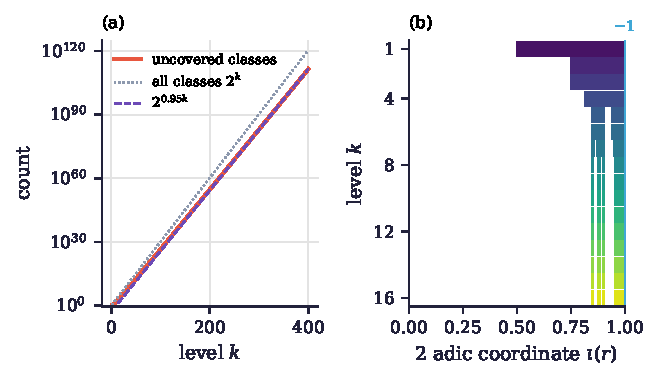
\includegraphics[width=\textwidth]{figures/ch10b_sieve.pdf}
\caption{The residue sieve. (a) The number of classes modulo $2^k$ not certified
to descend within $k$ steps, computed exactly up to $k=400$, against all $2^k$
classes and the growth rate $2^{0.95k}$. (b) The uncovered classes at levels
$1$ to $16$ drawn in the $2$ adic coordinate $\iota(r)=\sum r_i2^{-i-1}$; they
shrink to a closed set of measure zero that contains $-1$, the point at the
right edge, whose orbit never descends.}
\label{fig:ch10b:sieve}
\end{figure}

\Cref{thm:ch5c:residue} gives the same conclusion from the side of
optimization: the residue graph has cycles of positive mean weight, so no potential $\log x+\varphi(x\bmod2^k)$ with bounded $\varphi$ decreases at every step for all large $x$.
The structural reason is $2$ adic. Let $E\subset\Z_2$ be the set of $2$ adic
integers whose parity sequence under $T$ satisfies $3^{m_j}>2^j$ for every $j$,
the points with infinite coefficient stopping time.

\begin{proposition}[What residue certificates can and cannot do]
\label{prop:ch10b:residue}
\leavevmode
\begin{enumerate}[label=(\roman*),leftmargin=2em]
\item $E$ is a closed subset of $\Z_2$ of Haar measure zero, it is the
  intersection over $k$ of the unions of uncovered classes at level $k$, and it
  contains $-1$, $-5$ and $-17$, one point of each of the three known cycles of $T$ on the negative
  integers.
\item Every uncovered class at every level contains infinitely many positive
  integers. Hence no residue certificate of finite level covers all integers
  $n\ge2$.
\item If a positive integer $n\ge2$ lies in $E$, its orbit never falls below
  $n$. Hence the descent form of the conjecture implies $E\cap\{2,3,\ldots\}=
  \emptyset$, and conversely this together with the coefficient stopping time
  conjecture of \cref{chap:parity} implies the descent form.
\end{enumerate}
\end{proposition}

\begin{proof}
(i) The uncovered set at level $k$, $E_k$, is a finite union of balls
$r+2^k\Z_2$, hence closed, and $E=\bigcap_kE_k$ because the parity vector of a
$2$ adic integer of length $k$ depends only on its class modulo $2^k$. Its
measure is $\lim_k(1-F(k))=0$ by \cref{thm:density}. The point $-1$ is fixed by
$T$ and odd, so $m_j=j$ and $3^j>2^j$ for all $j$. For a point of a negative cycle with $r$ odd steps in a period of $s$ steps,
$3^r>2^s$ by the reversed cycle identity\index{cycle identity} of \cref{chap:cycles}, so the ratio
$3^{m_j}/2^j$ is multiplied by $3^r/2^s>1$ over each period; hence it exceeds $1$
for every $j$ as soon as it does for $j\le s$, and a direct check over one period
confirms this for $-5$ (period $3$) and $-17$ (period $11$), though not for the
other points of those cycles. (ii) A class $r+2^k\Z$ contains
$r+2^kt$ for every $t\ge1$. (iii) If $n\in E$ then
$T^{(j)}(n)=(3^{m_j}n+c_j)/2^j>n$ for every $j$, since $c_j\ge0$. The converse uses
the conjecture of Terras that the coefficient stopping time equals the stopping
time for every $n\ge2$.
\end{proof}

The proposition isolates exactly what computation on residues can deliver: the descent form of the conjecture implies that no integer $n\ge2$ lies in the measure zero closed set $E$, and the converse holds if the coefficient stopping time conjecture of Terras\index{Terras, R.} holds (\cref{rem:ch2:cst}).
Positive integers are the
$2$ adic integers whose digits are eventually all $0$, while the known points of
$E$, such as $-1=\ldots1111$, have digits eventually all $1$ or eventually
periodic. The remaining statement is an integrality property, a statement about
how $E$ meets the eventually zero sequences, and no finite residue computation
can establish it, because every finite level leaves balls of $E_k$ that contain
both integers and points of $E$.

\section{Automated termination provers}\label{sec:ch10b:automated}

The most ambitious computational attack to date takes the certificate\index{certificate} idea to its
logical end. Yolcu\index{Yolcu, E.}, Aaronson\index{Aaronson, S.} and Heule\index{Heule, M. J. H.}~\cite{yolcu2023} encode the Collatz map as a
string rewriting\index{rewriting system} system acting on mixed binary and ternary representations,
prove that termination of the system is equivalent to the conjecture, and search
for termination proofs by matrix interpretations, a standard technique in which
each rewriting rule must decrease a weight computed by multiplying small
matrices. Their prover found automatic proofs of nontrivial weakenings of the
conjecture, but not of the conjecture itself.

In the language of this book a matrix interpretation is a Lyapunov function\index{Lyapunov function} of
a special kind: the weight of a word is a linear function of a product of
matrices indexed by its letters, so it is a potential that reads the digits of
$n$ through a finite automaton. \Cref{prop:ch10b:residue} explains why such
potentials face the same obstruction as residue certificates\index{residue sieve} when they read
only boundedly many digits, and why the mixed representation matters: a
ternary digit records information about $n$ that its binary residues do not, so
an automaton reading both can in principle see the integrality that separates
the positive integers from $E$. That is the most promising feature of the
approach, and the reason it is a natural place for the large scale computation
of a coming decade.

\section{Does the MM view offer guidance?}\label{sec:ch10b:guidance}

It does, in several specific ways.

\paragraph{The potential.} The martingale duality of \cref{chap:stochastic}
constrains the potential: in the Bernoulli model for $T$, $x_n$ itself has no drift\index{drift}, $\log x_n$ has drift
$\log(\sqrt3/2)$, and $x_n^\theta$ decreases in expectation exactly when $0<\theta<1$ (\cref{thm:martingale}).
Any certificate\index{certificate} whose leading term grows at least linearly in $n$, such as one built on $n$ or on $n^\theta$ with $\theta\ge1$, fights the martingale\index{martingale}, which is why linear majorizer\index{majorization}s fail (\cref{prop:mmfails}); the powers $n^\theta$ with $0<\theta<1$ decrease in expectation but, like $\log n$, only on average over residue classes.
Matrix interpretations
measure size multiplicatively, through products, which is the right
geometry.

\paragraph{The horizon.} \Cref{thm:nolyapunov,cor:ch4:multistride} and the comments after them show that no monotone certificate with a fixed horizon exists: for every $J$ there are integers whose first $J$ strides all ascend, which defeats every nondecreasing potential, and $S^{(J)}(5)=1$ for every $J\ge1$, which defeats every nonincreasing one. An MM certificate built on a monotone potential such as $\log x$ must
therefore majorize over a \emph{variable} horizon, the number of steps to the
first descent, which is the stopping time\index{stopping time}. The greedy scheme ``iterate until
the potential has decreased, then majorize afresh'' is exactly the stopping time
decomposition of \cref{chap:parity}, and the conjecture in descent form is the
statement that this greedy MM is well defined at every $n\ge2$. The MM language
thus turns the conjecture into a termination statement for a specific
algorithm, which is precisely the form a termination prover needs.

\paragraph{The switching.} For Switching MM the joint spectral radius of the two modes, computed exactly by \cref{prop:ch5b:jsr}, is below one at every parameter value computed, and at all values if \cref{conj:ch5b:transient} holds; every switching sequence is then safe (\cref{cor:ch5b:anyswitch}).
For the Collatz switched system\index{switched system}
\eqref{eq:ch5b:switched} the opposite holds: some switching sequences diverge, the all odd one for instance, and
by the theorem of Terras\index{Terras, R.} and Everett\index{Everett, C. J.} (\cref{thm:terras}) every parity word of every length is realized by a residue
class containing arbitrarily large integers. So there is no constraint on the
switching signal at any finite horizon, and the constrained switching methods
of control theory, which certify stability by restricting the admissible
switching sequences to the language of a finite automaton, have nothing to work
with. Whatever constrains the Collatz signal couples the parity sequence to the
size and the digits of the state. This is the switched systems form of
\cref{prop:ch10b:residue}.

\paragraph{The potential, pressed.} \Cref{chap:mmcollatz} pushes the
majorization idea to its limit and proves three impossibility results for potentials that decrease at every step: no potential $\log x+\varphi(x\bmod2^k)$ with bounded $\varphi$ decreases at every step for all large $x$, for any $k$, because the cycles of
$T$ on the negative integers\index{negative cycles} are positive cycles of every residue graph
(\cref{thm:ch5c:residue}); any pointwise potential that decreases at every stride must give integers with $j$
trailing ones a surplus growing like $j\log(3/2)$ (\cref{prop:ch5c:surplus});
and the block potentials that supply this surplus fail, in the model, at a fraction of odd
integers that no weight brings below $0.143$ (\cref{prop:ch5c:runpot}). The
same chapter shows that the cycle inequality is the bound of the multiplicative
majorizer\index{MM algorithm} summed around the cycle, so for the cycle half majorization is a
reformulation and not a method.

\paragraph{The memory.} Accelerated methods need Lyapunov functions of two
consecutive iterates (\cref{sec:ch5b:stability}), and one might hope that a
potential with memory, depending on the recent history of the orbit, could
certify Collatz descent.
A memory of bounded length, however, adds only boundedly many parities, since $x_{n-1}$ is determined by $x_n$ and the parity of $x_{n-1}$, and a potential $\log x_n+\varphi$ with $\varphi$ bounded, whatever part of that history and of the residues of $x_n$ it reads, still increases along the long runs of odd steps from integers $2$ adically close to $-1$, as in \cref{thm:ch5c:residue}.
Memory helps only if it records unbounded
arithmetic information, the digits that decide integrality.

\paragraph{Polyak.} A reader of \cref{chap:momentum,chap:difference} may ask
whether Polyak\index{Polyak, B. T.}'s results, which underlie the momentum method, have anything
to offer here. Four of them are relevant and none of them transfers. The heavy
ball method\index{heavy ball}~\cite{polyak1964} is what Switching MM specializes, and its analysis is exactly
the switched system of \cref{chap:difference}; it tells us how the Collatz
schedule behaves as an optimizer, not how the integers behave. The gradient
dominance, or Polyak and \L{}ojasiewicz\index{Lojasiewicz, S.@\L{}ojasiewicz, S.}, inequality\index{Polyak and Lojasiewicz@Polyak and \L{}ojasiewicz inequality}
$\|\nabla f\|^2\ge2\mu(f-f^\ast)$~\cite{polyak1987} is the condition that makes linear rates
possible without convexity, and it is a pointwise condition: it would require
$\log x$ to decrease at every step by a fixed fraction of its distance to the
minimum, which the ascents of \cref{thm:nolyapunov} rule out. The Collatz
drift is additive and holds only in expectation, which is Foster\index{Foster, F. G.}'s condition
for Markov chains, not Polyak's for descent methods. Polyak and Ruppert\index{Ruppert, D.}
averaging~\cite{ruppert1988,polyak1990,polyak1992}, the device by which a noisy iteration achieves the optimal rate by
averaging its iterates, corresponds under the logarithm to the Ces\`aro
criterion of \cref{chap:divergence}: it is the right object to look at and it
is the statement that remains unproved. Finally the Polyak step size
$\alpha_k=(f(x_k)-f^\ast)/\|\nabla f(x_k)\|^2$~\cite{polyak1987} needs the optimal value, which
for Collatz is $f^\ast=\log1=0$ and is known; but the Collatz step sizes are
not ours to choose, the parity sequence chooses them, and a method that
adapts its step to the distance from the optimum has nothing to adapt.
Polyak's results are therefore useful for the optimizer in Part II and
irrelevant to the conjecture in Part III, which is the same division the rest
of the book makes.

So the optimization reading does not shorten the path, but it marks it. It says
which potentials can work, that the horizon of a monotone certificate must be variable, that parity
information of bounded length can never suffice, and that the missing ingredient is an
integrality argument, a way of using the fact that $n$ has a terminating binary
expansion. These are also features of the most serious computational
programme now in existence.

\section*{Notes}

The $2$ adic formulation of the stopping time\index{stopping time} problem is due to Terras\index{Terras, R.} and to
Lagarias\index{Lagarias, J. C.}~\cite{lagarias1985}, and Bernstein\index{Bernstein, D. J.}~\cite{bernstein1994} gives a
noniterative form. The rewriting\index{rewriting system} approach and the matrix interpretation prover
are from Yolcu\index{Yolcu, E.}, Aaronson\index{Aaronson, S.} and Heule\index{Heule, M. J. H.}~\cite{yolcu2023}.
The residue sieve\index{residue sieve} counts to $k=400$ and the divisibility sieve experiment are ours.
The exponent $h=H(1/\lt)$ gives the decay rate $1-h$ of Lagarias\index{Lagarias, J. C.}'s exponential form of the density theorem of Terras\index{Terras, R.} and Everett\index{Everett, C. J.}, $1-F(k)\le2^{-(1-h)k}$~\cite[Theorem~D]{lagarias1985}.
\Cref{prop:ch10b:residue} in the form stated is ours, although each ingredient of the proposition is classical.

\section*{Exercises}

\begin{exercise}
Using the recursion of \cref{prop:ch2:dp}, show that the number of uncovered
classes modulo $2^k$ is equal to the number of binary words of length $k$ all of
whose prefixes have a proportion of ones above $1/\lt$, and deduce that it grows
like $2^{(h+o(1))k}$ with $h=H(1/\lt)$ (the binomial tail gives the upper bound).
\end{exercise}

\begin{exercise}
Run the divisibility sieve of \cref{sec:ch10b:cycles} for $(m,k)=(8,13)$ by
hand or by machine, find the residues of $c_{13}(w)$ modulo $233$ that occur, and
confirm that $0$ is not among them. How many words are there, and how does that
compare with $233$?
\end{exercise}

\begin{exercise}
Show that the rational number $1/5$ is periodic under the accelerated map\index{accelerated map} on
$\Z_2$ with odd denominators allowed, and decide whether it lies in $E$.
\end{exercise}

\begin{exercise}
Explain why a potential $V(n)=\log n+\varphi(n\bmod2^k)$ with $\varphi$ bounded
cannot certify descent over a fixed horizon $J$ for all $n\ge2$, by exhibiting
integers in the class $-1\bmod2^{J+1}$ for which $V$ increases over $J$ steps
once $n$ is large.
\end{exercise}

\chapter{Samplers and the Horizon}\label{chap:samplers}

\Cref{chap:computation} asked what computation can prove. This chapter asks what
simulation can find. The idea, suggested by the Bayesian computation
literature, is to treat the problem as one of rare event simulation. Define an energy on
the integers, say the total stopping time, declare the integers with high energy to
be the interesting ones, and use a sampler that climbs the energy landscape to
find them or to measure how many there are. Nested sampling\index{nested sampling}, the vertical
likelihood\index{vertical likelihood} sampler and split sampling\index{split sampling} are three such methods, all built to
estimate a normalizing constant by moving through a sequence of level sets
rather than by sampling the base measure directly, and, given exact draws from each level set, all three
reach regions of exponentially small prior mass in a number of steps that is
polynomial in the depth. The question this chapter answers is whether such a
method can say anything about the conjecture in polynomial time. It can do one
thing exactly, which we prove, and beyond a horizon a local sampler leaves the tree of merged orbits it starts in only about as often as rejection sampling finds a new one, which we explain heuristically in the Bernoulli model and observe in practice.

\section{One identity, three samplers}

Let $\pi$ be a probability measure on a space $\mathcal X$ and let
$L:\mathcal X\to[0,\infty]$ be an energy. Write
\[
  Z(m)=\pi\{L>m\},\qquad m\ge0,
\]
for the prior volume of the level set\index{level set} above $m$. The quantity every method
estimates is the expected energy, or more generally $\E_\pi[g(L)]$ for a
monotone $g$, through the layer cake identity
\begin{equation}\label{eq:ch10b:cake}
  \E_\pi[L]=\int_0^\infty Z(m)\,dm .
\end{equation}
The common device is a level variable. Fix a weight, a measure $\omega$ on $[0,\infty)$ with cumulative weight $W(l)=\omega([0,l))$ finite for every $l$, and consider the joint law
\begin{equation}\label{eq:ch10b:aug}
  \pi_\omega(dx,dm)\ \propto\ [\,L(x)>m\,]\,\pi(dx)\,\omega(dm) ,
\end{equation}
which is a probability law when its total mass $\int Z\,d\omega=\E_\pi[W(L)]$ is finite.
Its two marginals are read off at once: integrating out $m$ gives $x$ the law
proportional to $W(L(x))\pi(dx)$, and integrating out $x$ gives $m$ the law
proportional to $Z(m)\,\omega(dm)$. Polson\index{Polson, N. G.} and Scott\index{Scott, J. G.}~\cite{polsonscott2015} call a
Markov chain that alternates the two conditionals, $m$ given $x$ and $x$ given
$m$, a weighted slice sampler\index{slice sampling}, and show that vertical likelihood and nested sampling are choices of the weight; Birge\index{Birge, J. R.}, Chang\index{Chang, C.} and Polson~\cite{birge2013} show the same for split sampling.

\begin{enumerate}[label=(\roman*),leftmargin=2em]
\item \emph{Vertical likelihood.} Take the cumulative weight $W=1/Z$, that is a unit atom at $m=0$ together with the density $(1/Z)'$. The level marginal is then proportional to $-Z'(m)/Z(m)$ away from $0$, which is flat in the coordinate $\log(1/Z(m))$: the chain spends equal time in each factor $e$ of prior volume, and the $x$ marginal is $\pi$ reweighted by $W(L(x))=1/Z(L(x))$, which grows like $e^{DL}$ when $Z(m)\approx e^{-Dm}$. With this weight the augmented law has infinite mass when $L$ is continuous, since $Z(L)$ is then uniform on $(0,1)$, and Polson and Scott floor the weight, $W(m)=1/\max(\eta,Z(m))$, to keep the law proper~\cite[eq.~(19)]{polsonscott2015}. Since $Z$ is unknown one uses a running estimate $\hat Z$ in its place, and recovers $Z(m)$ from the chain by importance weighting each sample $x$ with $1/W(L(x))$.
  The conditional of $m$ given $x$
  is explicit: draw $T$ uniform on $(0,1/\max(\eta,Z(L(x))))$ and set $m=0$ if
  $T\le1$ and $m=Z^{-1}(1/T)$ otherwise~\cite[Lemma 3]{polsonscott2015}.
\item \emph{Nested sampling.} Skilling\index{Skilling, J.}~\cite{skilling2006} discretizes the
  same weight $W=1/Z$. A population of $N$ live points is drawn from
  $\pi$; at each iteration the point of lowest energy $L_i$ is removed and
  replaced by a draw from $\pi$ conditioned on $\{L>L_i\}$, obtained by running
  a $\pi$ invariant Markov kernel inside the level set. The prior volume above
  $L_i$ shrinks by a factor with mean $N/(N+1)\approx e^{-1/N}$, whose logarithm has mean exactly $-1/N$, per iteration,
  which is the flat level marginal in logarithmic coordinates, and
  \eqref{eq:ch10b:cake} is estimated by the quadrature
  $\sum_i(X_{i-1}-X_i)\,g(L_i)$ with $X_i=e^{-i/N}$.
\item \emph{Split sampling.} Birge, Chang and Polson~\cite{birge2013} fix the
  levels adaptively at quantiles instead: at stage $t$ the sampler runs inside
  $\{L>m_{t-1}\}$, sets $m_t$ to the $(1-\rho)$ quantile of the energies it
  sees, and records the conditional fraction $p_t\approx\rho$ above $m_t$. The
  product $\prod_{s\le t}p_s$ estimates $Z(m_t)$; this is the product estimator, which they show is split sampling with the discrete weights $\omega_t=1/Z(m_t)$ (their Theorem~1).
  If the stage estimates are independent with relative variances $v_t$, the relative variance of the product is $\prod_t(1+v_t)-1$; with $N$ independent samples per stage $v_t\approx(1-\rho)/(\rho N)$, and the product is about $t(1-\rho)/(\rho N)$, linear in the number of stages $t=\log(1/Z)/\log(1/\rho)$, when $N$ is large compared with $t$.
  The Rao
  Blackwellized estimate
  $\hat Z(m)=\sum_{x:L(x)>m}\Omega(L(x))^{-1}\big/\sum_x\Omega(L(x))^{-1}$,
  with $\Omega=W$ the cumulative weight actually used, recovers the whole curve $Z$ from
  one run; with $\Omega=1/Z$ the sampling distribution of the method matches that of nested sampling, which
  is their Theorem~2.
\end{enumerate}

In every case the work per sample is polynomial in the depth, provided one
ingredient: a kernel that moves freely inside each level set $\{L>m\}$. The
cost of a method is the cost of that kernel, and the obstruction we will meet
is that for the natural Collatz energy no local kernel moves freely at depth.

\section{The Collatz prior and two energies}

The only natural prior on the integers is the one the $2$ adic formulation
provides, the Haar measure $\mu$ on $\Ztwo$ of \cref{chap:parity}, under which
the residue modulo $2^k$ is uniform for every $k$ and the parity digits of the
orbit are independent fair coins (\cref{thm:terras}). Two energies suggest
themselves. The first is the coefficient stopping time $\tau$ of \cref{def:ch2:stopping}, the
first $k$ at which $3^{m_k}<2^k$, which is a function of the parity word of
length $k$ and so of the residue class modulo $2^k$. The second is the total
stopping time\index{stopping time} $\sigma_\infty$, the first $k$ with $T^{(k)}(n)=1$, counted in steps of $T$ (in \cref{chap:intro} the same symbol counts steps of $T_0$), which is the
quantity the conjecture is about. The two are separated by a horizon.

\begin{proposition}[Two energies]\label{prop:ch10b:horizons}
\leavevmode
\begin{enumerate}[label=(\roman*),leftmargin=2em]
\item For every $m$ the level set $\{\tau>m\}\subset\Ztwo$ is a union of
  residue classes modulo $2^m$, hence open and closed, and its Haar measure is
  $Z_\tau(m)=1-F(m)=2^{-m}\sum_jN_m(j)$, computable exactly in $O(m^2)$
  arithmetic operations by \cref{prop:ch2:dp}. The sets decrease in $m$ and
  their intersection $\{\tau=\infty\}$ has measure zero.
\item For every $m$ the set $\{x\in\Ztwo:\sigma_\infty(x)\le m\}$ is finite, and it contains at most one positive integer in each residue class modulo $2^m$.
  Consequently $\{\sigma_\infty>m\}$ has Haar measure one for every $m$, and so does the intersection $\{\sigma_\infty=\infty\}$ of these sets: the energy $\sigma_\infty$ is almost surely infinite under $\mu$, and any simulation with this energy must use a uniform prior on a finite range, which we take to be $[2,2^B)$, with $Z_\sigma(m)=\#\{2\le n<2^B:\sigma_\infty(n)>m\}/(2^B-2)$.
\end{enumerate}
\end{proposition}

\begin{proof}
(i) is the content of \cref{sec:ch2:terras} and \cref{prop:ch2:dp}: $\tau(n)>m$
is decided by the first $m$ parities, which are a bijective function of
$n\bmod2^m$, and the density theorem of \cref{chap:parity} says
$1-F(m)\to0$.
For (ii), every $y\in\Ztwo$ has exactly the two preimages $2y$ and $(2y-1)/3$ under $T$, so $\{\sigma_\infty\le m\}$, which lies in $\bigcup_{k\le m}T^{-k}(1)$, has at most $2^{m+1}-1$ points.
Now fix a parity word $w$ of length $m$ with $j$ ones. By the Terras formula $T^{(m)}(n)=(3^jn+c_w)/2^m$ for every $n$ in the class of $w$, and $\sigma_\infty(n)\le m$ forces $T^{(m)}(n)\in\{1,2\}$, because the orbit alternates between $1$ and $2$ once it reaches $1$; so $n=(2^m-c_w)/3^j$ or $n=(2^{m+1}-c_w)/3^j$.
These differ by $2^m/3^j$, so both are integers only when $j=0$; then $w$ is the zero word, $c_w=0$, and of $2^m$ and $2^{m+1}$ only the first has $\sigma_\infty\le m$.
Hence each class contains at most one positive integer with $\sigma_\infty\le m$, the complement of a finite set has full Haar measure, and so does a countable intersection of such complements.
\end{proof}

The horizon is the following. The event $\{\tau>m\}$ reads only the first $m$ parities, which are a bijective function of the residue modulo $2^m$, so its level sets have the clopen
structure a sampler needs: a residue class is a cylinder, and moving inside a
union of cylinders is easy. An integer below $2^B$, on the other hand, carries no residue information beyond its first $B$ parities, which determine it by Terras' bijection, so beyond its bit length its orbit has no unread bits, and on the box the level sets of $\sigma_\infty$ are sets of particular integers with no $2$ adic description at all.

\section{Perfect split sampling for the coefficient stopping time}

On the near side of the horizon simulation is not merely polynomial but exact.

\begin{theorem}[Perfect split sampling]\label{thm:ch10b:perfect}
Fix a depth $K\ge1$, let the levels be the integers $0\le k\le K$, let $Z_k=1-F(k)$ be the exact volumes
of \cref{prop:ch10b:horizons}(i), write $\tau_K=\min(\tau,K+1)$, and let the discrete weights be
\begin{gather*}
  \omega_0=1,\qquad \omega_k=\frac1{Z_k}-\frac1{Z_{k-1}}\quad(1\le k\le K),\\
  \text{so that}\qquad W(l)=\sum_{k<l}\omega_k=\frac1{Z_{l-1}}\quad(1\le l\le K+1) .
\end{gather*}
Then the augmented law
$\pi_\omega(x,k)\propto[\tau_K(x)>k]\,\mu(dx)\,\omega_k$ has the finite mass $1+\sum_{k=1}^K\lambda_k$, where $\lambda_k=Z_k\omega_k=1-Z_k/Z_{k-1}$ is the hazard, and its Gibbs sampler can be run exactly, with
no Markov chain inside the level sets:
\begin{enumerate}[label=(\roman*),leftmargin=2em]
\item given $x$, the level $k$ is drawn from $\omega$ restricted to
  $\{0,\dots,\tau_K(x)-1\}$, a finite discrete law;
\item given $k$, a point with law $\mu$ restricted to $\{\tau>k\}$ is drawn exactly, as far as $\tau_K$ can see it, which is to say its residue modulo $2^K$. An alive word of length $k$ is drawn uniformly by
  backward sampling of the dynamic programme of \cref{prop:ch2:dp}: starting
  from the terminal count $N_k(j)$ chosen with probability
  $N_k(j)/\sum_{j'}N_k(j')$, the parities are generated from the last to the
  first with the probability $N_{i-1}(j)/N_i(j)$ of a zero and
  $N_{i-1}(j-1)/N_i(j)$ of a one. The word is followed by $K-k$ independent fair parities, and the word of length $K$ is converted to a residue modulo $2^K$ by the Terras bijection. The cost is $O(K)$ per draw after an $O(K^2)$ table, since step (i) reads $\tau_K(x)$ from the word itself.
\end{enumerate}
The level marginal of the chain is proportional to $1$ at $k=0$ and to $\lambda_k$ for $1\le k\le K$, and the
$x$ marginal is proportional to $\mu$ weighted by $1/Z_{\tau_K(x)-1}$, so that the event $\{\tau>K\}$ has stationary probability $1/(1+\sum_{k\le K}\lambda_k)$. Every $k\le K$ with
$R_k>0$, in the notation of \cref{prop:ch2:dp}(ii), is visited with the positive frequency $\lambda_k/(1+\sum_{k'\le K}\lambda_{k'})$. Without the truncation the augmented law has infinite mass, since $\prod_{k\le K}(1-\lambda_k)=Z_K\to0$ forces $\sum_k\lambda_k=\infty$, and every level is then visited with long run frequency zero.
\end{theorem}

\begin{proof}
The weights are nonnegative because $Z$ is nonincreasing, and $W$ telescopes as
stated. The conditional of $k$ given $x$ is $\omega$ restricted to $k<\tau_K(x)$
by \eqref{eq:ch10b:aug}; the conditional of $x$ given $k\le K$ is $\mu$ restricted
to $\{\tau_K>k\}=\{\tau>k\}$. Under $\mu$ the parities are independent fair coins (\cref{thm:terras}), so under this conditional law the first $k$ parities form a uniform alive word of length $k$, the later parities are independent fair coins, and $\tau_K$ depends only on the first $K$ of them, that is on the residue modulo $2^K$. The counts $N_i(j)$ of \cref{prop:ch2:dp} count the alive
words of length $i$ with $j$ ones, and a word is alive if and only if every
prefix is alive, so the stated backward probabilities are the exact
conditionals of a uniformly chosen alive word, by induction on $i$. The
marginals follow from \eqref{eq:ch10b:aug}: the event $\{\tau>K\}$ has $\mu$ measure $Z_K$ and weight $W(K+1)=1/Z_K$.
The level process is itself a Markov chain, since the point drawn at level $k$ is fresh, and it is reversible with respect to $\nu(k)=Z_k\omega_k$, because its transition probabilities satisfy $\nu(k)P(k,l)=\omega_k\omega_l\sum_{t>\max(k,l)}\mu\{\tau_K=t\}W(t)^{-1}$, which is symmetric in $k$ and $l$ (with $\tau$ in place of $\tau_K$ when there is no truncation). It is irreducible on the levels with $\nu(k)>0$, which are $0$ and the $k$ with $Z_k<Z_{k-1}$, that is with $R_k>0$, because $0$ is reached from every level in one step and every such level from $0$; and it is aperiodic, because it can stay at $0$. With the truncation $\nu$ has finite mass, and the ergodic theorem gives the stated frequencies. Without it $\nu$ has infinite mass; a positive recurrent chain would have a stationary probability law, which for an irreducible recurrent chain is the unique invariant measure up to a constant factor, and $\nu$ is not proportional to a probability law, so the chain is transient or null recurrent and every level has long run frequency zero.
\end{proof}

\begin{algorithm}[t]
\caption{Perfect split sampling for the coefficient stopping time}
\label{alg:perfectsplit}
\begin{algorithmic}[1]
\Require depth $K$, number of sweeps $S$
\State compute $N_i(j)$ for $i\le K$ by \cref{prop:ch2:dp}; set $Z_i=2^{-i}\sum_jN_i(j)$
\State set $\omega_0\gets1$ and $\omega_i\gets1/Z_i-1/Z_{i-1}$ for $1\le i\le K$
\State draw $x$, a uniform residue modulo $2^K$, and set $k\gets0$
\For{$s=1,\dots,S$}
  \State draw $k$ from $\{0,\dots,\min(\tau(x),K+1)-1\}$ with probability $\propto\omega_k$
    \Comment{level given point}
  \State draw $j$ with probability $N_k(j)/\sum_{j'}N_k(j')$
    \Comment{number of odd steps}
  \For{$i=k,k-1,\dots,1$}
    \State with probability $N_{i-1}(j)/N_i(j)$ set $w_i\gets0$, else $w_i\gets1$ and $j\gets j-1$
  \EndFor
  \State $x\gets$ the residue modulo $2^K$ whose parity word is $w_1\cdots w_k$ followed by $K-k$ fair parities (Terras)
    \Comment{point given level}
  \State record $(x,k)$
\EndFor
\end{algorithmic}
\end{algorithm}

The theorem is a complete answer to the simulation question on the near side
of the horizon. \Cref{alg:perfectsplit} states the chain in full. We ran it at depth $K=400$ for twenty thousand sweeps, and \cref{fig:ch10b:montecarlo}(b) shows the first three thousand.
The level moves up at $46\%$ of the sweeps and down at $46\%$, with mean $167$ (the stationary mean is $157$); its maximum $400$ is the depth $K$ of the run, not a property of the walk.
A rejection sampler would need $1/Z_{400}\approx8.6\times10^8$ draws from $\mu$ to see one residue with $\tau>400$. The chain returns such a residue in $5.6\%$ of its sweeps, about one in eighteen (the stationary probability is $1/(1+\sum_{k\le400}\lambda_k)=0.049$), each sweep costing $O(K)$, and each such residue is an exact uniform draw from the residues modulo $2^{400}$ with $\tau>400$; the level itself reaches the top level $400$ in about one sweep in four hundred. That is
polynomial time sampling of a set of exponentially small measure, and the
samples are exact, not approximate. It is also, we stress, information already
contained in \cref{prop:ch2:dp}, whose backward sampling at the single level $400$ gives independent exact draws at the same cost: the Monte Carlo is a way of exploring the
nest, not of measuring it.

Panel (a) of the figure gives the volumes themselves. On the stopping levels
$k=\lfloor j\lt\rfloor+1$, the $k$ with $R_k>0$ by \cref{prop:ch2:dp}(ii), the hazard $\lambda_k=1-Z_k/Z_{k-1}$ is positive
and elsewhere it is zero, so $Z_\tau$ is a staircase; over $100\le k\le400$ it
follows the fit $Z_\tau(k)\approx Ck^{-1.355}e^{-Dk}$ with
\[
  D=\log2-H\bigl(1/\lt\bigr)=0.03469,
\]
the Chernoff rate for the proportion of ones in a fair word to exceed
$1/\lt$, where $H$ is the entropy in nats; in terms of the residue sieve exponent
$h=0.95$ of \cref{sec:ch10b:divergence}, $D=(1-h)\log2$, since $2^{(h-1)k}=e^{-Dk}$.
The polynomial correction is the ballot factor, of order $k^{-3/2}$ asymptotically by the heuristic of \cref{sec:ch2:density}; the fitted exponent is smaller at these depths, and in the exact recursion it rises to $1.48$ over $1000\le k\le6000$ and $1.50$ over $6000\le k\le20\,000$.
On the stopping levels with $100<k\le400$ the hazard averages $0.063$ ($0.055$ over $100<k\le6000$), against the value $1-e^{-D\lt}=0.053$
that a pure exponential with one stopping level every $\lt$ steps would give; the excess
is the polynomial factor, which makes the staircase steeper than exponential
at finite depth. One consequence is a
precise statement about which expectations exist: the partition function\index{partition function}
$\E_\mu[e^{\beta\tau}]=\sum_k(Z_{k-1}-Z_k)e^{\beta k}$ converges if and only if
$\beta\le D$.
It diverges for $\beta>D$, because it is at least $e^{\beta k}Z_k$ for every $k$ and $Z_k=e^{-Dk+o(k)}$, the exponent of \cref{thm:density} being sharp (\cref{sec:ch2:density}).
At $\beta=D$ it converges: write $X_k=m_k\log3-k\log2$, a random walk under $\mu$ with steps $\log(3/2)$ and $-\log2$, so that $\tau$ is the first $k$ with $X_k<0$; the step $\xi$ has $\E e^{\theta\xi}$ minimal at $\theta_*=0.488$, where it equals $e^{-D}$, so $e^{\theta_*X_k+Dk}$ is a martingale, and since $-\log2\le X_\tau<0$ optional stopping gives $\E_\mu[e^{D\tau}]\le2^{\theta_*}=1.40$ (the exact recursion to depth $20\,000$ gives about $1.25$).
So a Boltzmann weighting of the coefficient stopping time has a finite
temperature barrier at $\beta=D$, and no annealing\index{annealing} scheme can be run past it.
The expected coefficient stopping time itself is $\E_\mu[\tau]=\sum_kZ_k=3.4927$, the
layer cake sum of the staircase.

\section{Beyond the horizon: the total stopping time}

On the far side the picture changes, and not in the way one first expects. The
naive prediction is that a local move in $n$, a change of one bit, produces an
integer whose orbit is unrelated to the orbit of $n$ beyond the bit length, so
that inside a deep level set every proposal is rejected with probability about
$1-Z_\sigma(m)$ and the sampler is a rejection sampler. That prediction is
wrong, and the reason it is wrong is the first structural fact about
$\sigma_\infty$ that simulation reveals: orbits of nearby integers merge.

\begin{lemma}[Merging]\label{lem:ch10b:merge}
For every $k\ge0$, $T^{(3)}(8k+4)=T^{(3)}(8k+5)=3k+2$. More generally, if
$n\equiv n'\pmod{2^i}$ then the first $i$ parities of $n$ and $n'$ agree and
\[
  T^{(i)}(n')-T^{(i)}(n)=3^{j}\,\frac{n'-n}{2^i},
\]
where $j$ is the number of odd steps among the first $i$ (\cref{lem:ch2:perturb}). In particular
flipping bit $i$ of $n$ moves the orbit at step $i$ by exactly $\pm3^j$; and if at some step the two orbits occupy a pair $\{8k+4,8k+5\}$ with $k\ge1$, they coincide three steps later, so that $\sigma_\infty(n')=\sigma_\infty(n)$.
\end{lemma}

\begin{proof}
$8k+4\mapsto4k+2\mapsto2k+1\mapsto3k+2$ and $8k+5\mapsto12k+8\mapsto6k+4\mapsto3k+2$.
For $k\ge1$ none of these values is $1$ or $2$, so if the two orbits are at $8k+4$ and $8k+5$ after $s$ steps, neither has reached $1$, and both total stopping times equal $s+3+\sigma_\infty(3k+2)$; for $k=0$ the clause fails, since $\sigma_\infty(4)=2$ and $\sigma_\infty(5)=4$.
The general formula is \cref{lem:ch2:perturb}, or the Terras affine form $T^{(i)}(n)=(3^jn+c_w)/2^i$
applied to two integers in the same class of $w$.
\end{proof}

Merging is the mechanism that makes the Collatz graph a tree with many
confluences rather than a bundle of separate paths, and it is why $12$ and $13$ both reach $5$, and $28$ and $29$ both reach $11$, after three steps. For a sampler it has
a precise consequence.

\begin{proposition}[Coalescence]\label{prop:ch10b:acceptance}
Let $n$ and $n'$ be positive integers whose orbits meet at a point $x\ge3$, reached from $n$ after $s$ steps and from $n'$ after $s'$ steps. Then $\sigma_\infty(n')=\sigma_\infty(n)-s+s'$. In particular, if $s=s'$, as for the merging pairs of \cref{lem:ch10b:merge}, then $n'$ lies in every level set $\{\sigma_\infty>m\}$ that contains $n$.
\end{proposition}

\begin{proof}
An orbit that reaches $1$ stays in $\{1,2\}$ from then on, so neither orbit reaches $1$ before it reaches $x$. Hence $\sigma_\infty(n)=s+\sigma_\infty(x)$ and $\sigma_\infty(n')=s'+\sigma_\infty(x)$.
\end{proof}

The condition $s=s'$ matters. The integers $27$ and $31$ differ in one bit and their orbits meet, since $27\mapsto41\mapsto62\mapsto31$, but with $s=3$ and $s'=0$, so $\sigma_\infty(31)=\sigma_\infty(27)-3=67$, and $31$ is not in the level set $\{\sigma_\infty>69\}$ that contains $27$.
Fix a threshold $R$ and call two integers of $\{\sigma_\infty>m\}$ equivalent if their orbits pass through a common point of remaining stopping time at least $m-R$; the classes of this relation are the \emph{coalescence classes} of the level set, and we take $R=100$ below.

\begin{remark}[Coalescence or independence, a heuristic]\label{rem:ch10c:coalescence}
Let $n<2^B$ lie in $\{\sigma_\infty>m\}$ and let $n'$ differ from $n$ in one bit. If the orbits of $n$ and $n'$ meet at a point of remaining stopping time at least $m-R$, \cref{prop:ch10b:acceptance} gives $\sigma_\infty(n')$, and $n'$ joins the class of $n$ when $s=s'$. If they do not, the first $B$ parities of $n'$ determine it, and the Bernoulli model of \cref{chap:stochastic} treats the later parities of its orbit as fair coins independent of the orbit of $n$. The model probability that $n'$ lies in the level set is then about $Z_{\mathrm{mod}}(m-B)$, where $Z_{\mathrm{mod}}$ is the tail of the total stopping time in the model, and $Z_{\mathrm{mod}}(m-B)\sim e^{DB}Z_{\mathrm{mod}}(m)$ as $m\to\infty$, because in the model the total stopping time is a first passage time of the same random walk as $\tau$ and has the same rate $D$.
So a kernel of single bit flips restricted to $\{\sigma_\infty>m\}$ should leave the coalescence class of its starting point only at proposals of probability of order $e^{DB}Z_\sigma(m)$, with the census value $Z_\sigma$ standing in for the model tail.
This is a heuristic and not a theorem: the independence after step $B$ is an assumption of the model, and nothing here controls when the orbits of two integers meet.
\end{remark}

Both halves of the dichotomy are visible in the data. Panel (a) of
\cref{fig:ch10b:acceptance} shows, for each level $m$, the fraction of single
bit flips of integers in the level set on $[2,2^{26})$ that stay in it. Flips of the thirteen high bits behave as the naive prediction
suggests: their acceptance falls with $Z_\sigma(m)$ and is zero from $m=380$ on,
because a change high in the binary expansion displaces the orbit by $3^j$
with $j$ large, and such a displacement rarely lands on a merging pair.
Flips of the thirteen low bits accept at a rate that falls only slowly, from $18\%$ at $m=200$ to about $5\%$ between $m=360$ and $m=420$, while $Z_\sigma$ falls by more than four orders of magnitude: those are the coalescences.
At $m=400$ the overall acceptance is $2.6\%$ against the acceptance rate $3.8\times10^{-6}$ of rejection sampling, a factor of nearly seven thousand, and every one of the accepted moves stays in the coalescence class of its starting point (with the threshold $R=B=26$ in place of $R=100$, $170$ of the $172$ do).

\begin{figure}[t]
\centering
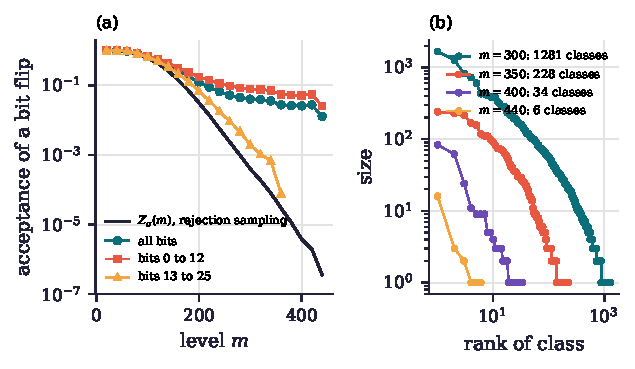
\includegraphics[width=\textwidth]{figures/ch10c_acceptance.pdf}
\caption{Coalescence or independence. (a) Acceptance rate of a single bit flip
inside the level set $\{\sigma_\infty>m\}\cap[2,2^{26})$, for all bits, for the
low bits and for the high bits, against the acceptance rate $Z_\sigma(m)$ of rejection sampling. Low
bit flips coalesce and keep accepting; high bit flips rarely coalesce and
stop. (b) Sizes of the coalescence classes of the level sets at
$m=300,350,400,440$, ranked. The $257$ integers above $400$ form $34$ classes,
$83$ of them in the largest; the $24$ above $440$ form six.}
\label{fig:ch10b:acceptance}
\end{figure}

At the deepest levels the confinement is exact in the data.
\Cref{tab:ch10b:clusters} decomposes each level set into coalescence classes,
two integers being in the same class if their orbits meet at a point whose
remaining stopping time is at least $m-100$ (the meeting point may lie above the
box, and usually does). The $26\,708$ integers above $300$
fall into $1\,281$ classes, the largest with $1\,659$ members; the $257$ above
$400$ fall into $34$, with $83$ in the largest; the $24$ above $440$ fall into
six. And of the $172$ accepted single bit flips among the integers above $400$ (the $86$ pairs that differ in one bit, each counted in both directions), all $172$ stay in the same class.
Not one crosses between classes, as the heuristic suggests, since a
crossing would be an independent orbit of length above $400$ found by a single
proposal.
At $m=300$ and $m=350$ some accepted flips do cross, $1\,112$ of $27\,896$ and $22$ of $2\,848$, that is $1.6\times10^{-3}$ and $2.5\times10^{-4}$ of all proposals, against the values $9.8\times10^{-4}$ and $1.3\times10^{-4}$ of $e^{DB}Z_\sigma(m)$ in the heuristic.

\begin{table}[t]
\centering\small
\caption{Coalescence classes of the level sets $\{\sigma_\infty>m\}$ on
$[2,2^{26})$, two integers being equivalent if their orbits merge no later than the point where the remaining stopping time equals $m-100$. The last two columns count the accepted single bit flips, that is the ordered pairs of integers in the level set that differ in one bit, and how many of them stay in the same class.}
\label{tab:ch10b:clusters}
\begin{tabular}{@{}rrrrrr@{}}
\toprule
$m$ & integers & classes & largest & accepted flips & same class \\
\midrule
$300$ & $26\,708$ & $1\,281$ & $1\,659$ & $27\,896$ & $26\,784$ \\
$350$ & $3\,432$ & $228$ & $240$ & $2\,848$ & $2\,826$ \\
$400$ & $257$ & $34$ & $83$ & $172$ & $172$ \\
$440$ & $24$ & $6$ & $16$ & $8$ & $8$ \\
\bottomrule
\end{tabular}
\end{table}

This is the right description of the far side of the horizon. A deep level set
is not a sparse set of unrelated integers; it is a small number of trees, each
the set of all tributaries of one slow orbit, and a local sampler stays in the tree it starts in, leaving it only rarely, at a rate per proposal of the order of the acceptance rate of rejection sampling. Inside the tree it is confined further, to the few members within a few bit flips of its current point: the $86$ pairs that differ in one bit join the $257$ integers above $400$ into at least $171$ separate pieces, and each stalled stage of split sampling reported below visited between one and twenty three distinct integers. The number of trees is what shrinks with
the depth, not the acceptance rate: $34$ at $400$, six at $440$. A level set
sampler therefore does not degrade into rejection sampling. It does something
more specific. It stays in the tree it starts in, and in fact among a handful of its members, and it
cannot climb above the maximum of $\sigma_\infty$ on that tree, because every
integer it can reach shares the tail of the same orbit. Its depth is bounded
by the deepest tree its initial population happens to contain, and new trees
are found only by independent draws from the prior or by the rare crossing proposals, at about the acceptance rate of rejection sampling.

How the trees multiply with the size of the box is shown in
\cref{tab:ch10b:trees}, which repeats the decomposition on $[2,2^B)$ for
$B=22,24,26$. At a fixed level and over $22\le B\le26$ the number of trees grows with $B$ at a rate
between $2^{B}$ and $2^{1.4B}$, faster at deeper levels, while the mean tree
size grows roughly like $2^{0.4B}$ and, at fixed $B$, falls steadily with the depth,
from $208$ at $m=200$ to $7.6$ at $m=400$ for $B=26$.
These are local exponents: at a fixed level the number of trees is bounded in $B$, since each tree has its own root, an integer with $\sigma_\infty=m-100$, and all such integers are at most $2^{m-100}$, because a step of $T$ at most halves.
A tree is the set of
predecessors below $2^B$ of one point $x$ at remaining depth $m-100$ that lie
more than a hundred steps above $x$, so its size is a count on the inverse tree
of \cref{chap:difference} and the number of trees is the number of such points
$x$ that are reached from the box by an orbit segment of more than a hundred steps. At the deeper levels the root $x$ usually lies above the box: at $m=400$ the roots of the two largest trees are
$146\,053\,012$ and $1\,330\,038\,578$, well beyond $2^{26}$, because a slow
orbit of a box integer climbs out of the box long before its remaining stopping
time falls to $300$. The trees are also mostly tributary: of the $83$ members
of the largest tree at $m=400$ only $14$ lie on the orbit of its deepest member,
the rest being integers whose orbits join that orbit later.

The deepest member of a tree is sometimes a delay record of \cref{chap:intro} (for $2$ of the $34$ trees at $m=400$), but
the correspondence is loose. At $m=400$ three of the $34$ trees contain a
record, including the two largest, whose deepest members are $55\,285\,737$
($\sigma_\infty=446$) and the record $36\,791\,535$ ($466$); the overall
record $63\,728\,127$, with $\sigma_\infty=592$, is a tree of one member at
$m=440$, because its orbit leaves the box at once and nothing below $2^{26}$
joins it in time. The records are the deepest trunks; the large trees are the
trunks that stay low enough, for long enough, to collect tributaries. A naive
model of tree size, in which each backward path of $d$ steps with $j$ odd
steps from $x$ exists with the integrality probability $3^{-j}$, predicts
fewer than four members for every root at $m\ge350$ and is wrong by three orders of magnitude or more: the median ratio of observed to predicted size is about $1.6\times10^3$ at $m=350$ and $10^4$ at $m=400$, where the largest tree has $83$ members against a prediction of $0.012$. Conditioned on being reached from the box by a slow orbit, a
root is reached by many, and the conditioning is the likely explanation. We do not
have a model that predicts either the number of trees or their sizes, and we
record the question as project P9 of \cref{chap:open}.

\begin{table}[t]
\centering\small
\caption{Trees of slow integers on $[2,2^B)$: the number of integers with
$\sigma_\infty>m$, the number of coalescence classes, and their mean and
largest size, for three box sizes.}
\label{tab:ch10b:trees}
\setlength{\tabcolsep}{4pt}\begin{tabular}{@{}rrrrrr@{}}
\toprule
$B$ & $m$ & integers & trees & mean size & largest \\
\midrule
$22$ & $200$ & $36\,482$ & $647$ & $56.4$ & $2\,224$ \\
$22$ & $250$ & $2\,558$ & $204$ & $12.5$ & $198$ \\
$22$ & $300$ & $201$ & $29$ & $6.9$ & $65$ \\
$24$ & $200$ & $291\,361$ & $2\,539$ & $114.8$ & $15\,153$ \\
$24$ & $250$ & $28\,429$ & $1\,047$ & $27.2$ & $1\,320$ \\
$24$ & $300$ & $2\,610$ & $184$ & $14.2$ & $381$ \\
$24$ & $350$ & $259$ & $33$ & $7.8$ & $42$ \\
$26$ & $200$ & $2\,125\,551$ & $10\,235$ & $207.7$ & $110\,856$ \\
$26$ & $250$ & $253\,975$ & $5\,682$ & $44.7$ & $8\,424$ \\
$26$ & $300$ & $26\,708$ & $1\,281$ & $20.8$ & $1\,659$ \\
$26$ & $350$ & $3\,432$ & $228$ & $15.1$ & $240$ \\
$26$ & $400$ & $257$ & $34$ & $7.6$ & $83$ \\
\bottomrule
\end{tabular}
\end{table}

\section{The three samplers against the census}

We tested the three samplers on the prior uniform on $[2,2^{26})$, with energy
the total stopping time of $T$ and the exact $Z_\sigma$ from the census of
\cref{chap:stochastic} (the maximum is $\sigma_\infty=592$, at
$n=63\,728\,127$). Each sampler had a budget of at most $2\times10^5$ energy evaluations per run, and the level set samplers used a kernel step that flips one to three random bits. Naive sampling used exactly $2\times10^5$ independent draws; nested sampling ran $200$ live points for $1600$ iterations with $120$ kernel steps per replacement ($192\,200$ evaluations); split sampling took $1200$ samples per stage, ten kernel steps apart, with $\rho=e^{-1}$, and stopped at the first stage that found no sample above its quantile (between $105\,300$ and $176\,510$ evaluations); and the vertical likelihood sampler ran $12\,000$ sweeps of $16$ kernel steps ($192\,000$ evaluations) with a floor $\eta=10^{-7}$ and the running estimate of $Z$ refreshed every $2000$ sweeps.
\Cref{tab:ch10b:mc} reports the medians of six independent runs.

\begin{table}[t]
\centering\small
\caption{Estimates of $Z_\sigma(m)=\Prob\{\sigma_\infty>m\}$ on $[2,2^{26})$,
medians of six runs at a budget of at most $2\times10^5$ energy evaluations each. The
exact values are from the census. From $m=400$ on, nested and split sampling report the prior mass of their last level, the vertical likelihood estimate is zero in four of the six runs at $m=400$, and so in the median, and in all six at $m=450$ and $500$, and naive sampling sees at most two integers above $400$ in a run and none above $450$.}
\label{tab:ch10b:mc}
\setlength{\tabcolsep}{4pt}\begin{tabular}{@{}rlllll@{}}
\toprule
$m$ & exact & naive & nested & split & vertical \\
\midrule
$100$ & $6.13\times10^{-1}$ & $6.13\times10^{-1}$ & $6.47\times10^{-1}$ & $4.57\times10^{-1}$ & $5.21\times10^{-1}$ \\
$200$ & $3.17\times10^{-2}$ & $3.18\times10^{-2}$ & $3.37\times10^{-2}$ & $3.25\times10^{-2}$ & $1.25\times10^{-2}$ \\
$300$ & $3.98\times10^{-4}$ & $3.75\times10^{-4}$ & $4.56\times10^{-4}$ & $1.94\times10^{-4}$ & $3.85\times10^{-5}$ \\
$400$ & $3.83\times10^{-6}$ & $5.0\times10^{-6}$ & $3.35\times10^{-4}$ & $2.54\times10^{-5}$ & $0$ \\
$450$ & $1.04\times10^{-7}$ & $0$ & $3.35\times10^{-4}$ & $2.54\times10^{-5}$ & $0$ \\
$500$ & $1.49\times10^{-8}$ & $0$ & $3.35\times10^{-4}$ & $2.54\times10^{-5}$ & $0$ \\
\bottomrule
\end{tabular}
\end{table}

\begin{figure}[t]
\centering
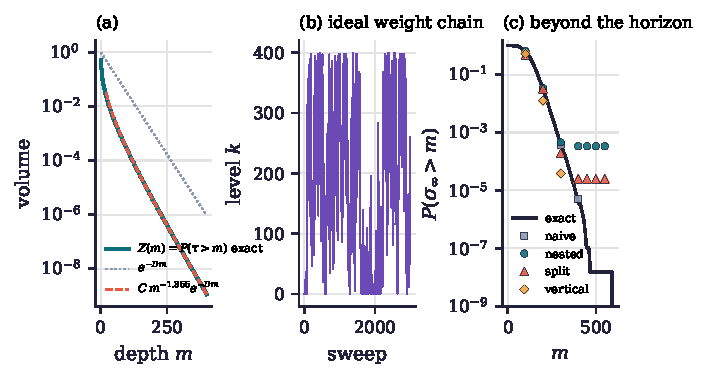
\includegraphics[width=\textwidth]{figures/ch10c_montecarlo.pdf}
\caption{Simulation on both sides of the horizon. (a) The exact staircase
$Z_\tau(m)=\Prob\{\tau>m\}$ under Haar measure, against $e^{-Dm}$ and the fit
$Cm^{-1.355}e^{-Dm}$ over $100\le m\le400$. (b) The level of the perfect split sampler of
\cref{thm:ch10b:perfect} at depth $K=400$, over the first $3000$ of twenty thousand sweeps: a free random walk on
the stopping levels up to the depth $400$ of the run, where the prior mass is
$1.2\times10^{-9}$. (c) The same methods applied to the total stopping time on
$[2,2^{26})$: exact $Z_\sigma$ against the medians of naive, nested, split and
vertical likelihood estimates. Naive and nested sampling track the truth to depth $300$, split sampling within a factor of about two there, and the vertical likelihood sampler only to depth $200$, within a factor of $2.5$; beyond depth $300$ the level set estimates stop changing or vanish.}
\label{fig:ch10b:montecarlo}
\end{figure}

Up to $m=200$ all four estimates agree with the truth to within a factor of about two and a half.
At $m=300$, where $Z_\sigma$ is $4\times10^{-4}$ and the budget contains some eighty naive hits, naive and nested sampling are within $15\%$ of the truth and split sampling is low by a factor of about two, while the vertical likelihood estimate is already low by a factor of ten; the level set methods bring nothing here, because the levels are still cheap.
Beyond $m=300$ the level set samplers stop, for two different reasons.
Split sampling stopped in every run at a level between $303$ and $338$, in a stage whose chain never left one coalescence class: it visited between one and twenty three distinct integers, all with the same total stopping time, so that no sample lay above the quantile. That is the confinement of the tree picture, and the estimate beyond that level is the product of the stage fractions found so far.
Nested sampling stopped for want of budget: its $1600$ iterations shrink the prior volume to $e^{-1600/200}=3.35\times10^{-4}$, which its six runs reached at thresholds between $297$ and $322$, and its estimate of $Z_\sigma(m)$ for every $m$ above the last threshold is that final volume.
At the end its live points occupied between $12$ and $36$ of the $573$ to $1\,331$ coalescence classes at the final threshold, and in every run some occupied class had a member above $400$, the deepest lying between $419$ and $466$; reaching $m=400$, where $Z_\sigma=e^{-12.5}$, would have needed about $2500$ iterations, more than the budget allows, so the table does not show whether nested sampling would be trapped in its trees.
The vertical likelihood chain visited energies up to between $381$ and $446$ in the six runs, but four runs never went above $400$, so its median estimate there is zero.
Naive sampling by contrast sees about one integer above $400$ per run, since $2\times10^5\times3.8\times10^{-6}\approx0.8$ (the six runs see $2$, $1$, $1$, $0$, $2$ and $0$), and is the best of the four there, because an independent draw is not confined to a tree.
The compression factors that make nested and split sampling
polynomial in the depth presuppose that the constrained kernel delivers an
independent point of the level set; in the stage where split sampling stopped it delivered another tributary of the same orbit, or the same integer again.

The expected value that \eqref{eq:ch10b:cake} delivers in this setting is the
mean total stopping time on the box, $\E[\sigma_\infty]=116.9$ at $B=26$, and
the Boltzmann evidence $\E[e^{\beta\sigma_\infty}]$, which nested sampling
(a separate run with $400$ live points, $6000$ iterations and $20$ single bit flips per replacement, script \texttt{ch10b\_nested.py}) estimates at $\beta=0.02$ as $16.2$ against the exact $15.4$: good enough, and
irrelevant, because both are averages over the integers that do reach $1$.

\section{What simulation can and cannot decide}

We can now state the verdict with some precision.

\begin{enumerate}[label=(\roman*),leftmargin=2em]
\item The conjecture is a universal statement: no positive integer lies in every set of the nest $\{\sigma_\infty>m\}$. A sampler explores the nest at finite depth.
  Under Haar measure this nest carries no signal at any depth: every $\{\sigma_\infty>m\}$ has measure one by \cref{prop:ch10b:horizons}(ii), and so does the limit $\{\sigma_\infty=\infty\}$, which contains $0$ and every negative integer; the positive integers in the limit form a countable set, hence a Haar null set, and the conjecture says that there are none.
  The residue nest $\{\tau>m\}$, which a sampler can navigate, decreases to the set $E=\{\tau=\infty\}$, which has Haar measure zero by \cref{prop:ch10b:horizons}(i), contains $-1$, $-5$ and $-17$, and contains no integer $n\ge2$ if the conjecture is true (\cref{prop:ch10b:residue}(iii)). Either way the target is a null set.
  No Monte Carlo method
  samples a null set, and a method that is polynomial in the depth is
  polynomial in a parameter that must go to infinity.
\item What simulation does in polynomial time is sample and measure the
  exceptional classes at depth $m$: the residues with $\tau>m$, exactly and
  with no Markov chain, by \cref{thm:ch10b:perfect}. These are the classes the
  residue sieve of \cref{sec:ch10b:divergence} enumerates, and the sampler is
  the randomized version of the sieve. Any computation that needs typical
  members of the exceptional classes, for instance to test a candidate
  potential or to seed a search for a certificate, has an exact tool.
\item Beyond the horizon, which is the bit length of the integers being
  sampled, a deep level set is a small number of trees of merged orbits
  (\cref{prop:ch10b:acceptance}, \cref{rem:ch10c:coalescence}, \cref{tab:ch10b:clusters}). A local sampler
  stays among a few members of one tree and leaves the tree only rarely, at about the acceptance rate of rejection sampling, so its depth is essentially the depth of the trees
  its initial population contains, and new trees are found by independent draws or by rare crossings, at about that rate.
  Estimating the number of slow integers below $2^B$ at levels where $Z_\sigma(m)$ is far below the reciprocal of the sampling budget therefore costs what it costs the
  census, and the census is exact.
\item The energy whose level sets a sampler can sample exactly at every depth is a function of a
  finite parity word; the energy the conjecture concerns is not. The gap
  between the two is the integrality gap of \cref{prop:ch10b:residue} once
  more: a sampler moves through residue classes, and the conjecture is about
  integers.
\end{enumerate}

So the answer to the question that opened this chapter is no. Simulation does
not decide the conjecture in polynomial time, or in any time, and the
obstruction is not one of efficiency but of what the level sets are. What
simulation offers, and this is worth having, is three things: the perfect
sampler of \cref{thm:ch10b:perfect} and the hazard description of the staircase,
which make the exceptional set at every finite depth a computable and
samplable object; the tree decomposition of the deep level sets, which says
that, in the boxes we computed, the slow integers are a small number of long orbits
together with their tributaries; and a heuristic account, borne out by the census, of why the one method
that moves freely between trees, independent sampling, is the one that costs
$1/Z_\sigma(m)$.

\section*{Notes}

Nested sampling\index{nested sampling} is Skilling's~\cite{skilling2006};
the vertical likelihood\index{vertical likelihood} view of it, and the weighted slice sampler that
places several level set methods in one scheme, are from Polson and Scott~\cite{polsonscott2015};
split sampling\index{split sampling}, with its Rao Blackwellized volume curve and its correspondences with the product estimator and with nested sampling, is from Birge, Chang and Polson~\cite{birge2013}; the slice sampler
itself is Neal's\index{Neal, R. M.}~\cite{neal2003}.
The weight $W=1/Z$ makes the level histogram flat in $\log(1/Z)$, while the flat energy histogram that the Wang\index{Wang, F.} and Landau\index{Landau, D. P.}\index{Wang and Landau algorithm} algorithm~\cite{wanglandau2001} aims at comes from weighting by the inverse density of states~\cite[Section~2]{polsonscott2015}.
The perfect sampler of \cref{thm:ch10b:perfect} is ours as a sampler, but its backward step is the classical recursive method of uniform generation from counts of Nijenhuis\index{Nijenhuis, A.} and Wilf\index{Wilf, H. S.}~\cite{nijenhuis1978}; the proposition on the two energies, the
coalescence heuristic and the tree decomposition of the deep level sets are
ours; the merging of consecutive integers under the map is classical (Garner\index{Garner, L. E.}~\cite{garner1985} used it to show that infinitely many pairs of consecutive integers have the same total stopping time) and is
the source of the confluences in every picture of the Collatz graph.

\section*{Exercises}

\begin{exercise}
Implement the backward sampler of \cref{thm:ch10b:perfect} and draw ten
residues modulo $2^{200}$ with $\tau>200$. Verify directly that each has more
than $200/\lt$ ones among its first $200$ parities, and estimate from a
thousand draws the mean number of ones at depth $200$. Compare with the
conditional law $j\mapsto N_{200}(j)/\sum_{j'}N_{200}(j')$.
\end{exercise}

\begin{exercise}
In the Bernoulli model of \cref{chap:stochastic}, show that the tail of the total stopping time has the same
exponential rate $D=\log2-H(1/\lt)$ as $\Prob\{\tau>m\}$, and explain why, in the model with starting points uniform on $[2,2^B)$, the box changes the prefactor but not the rate for $m\gg B$. (For the census itself $Z_\sigma(m)=0$ for $m\ge592$, the largest total stopping time in the box for $B=26$.)
\end{exercise}

\chapter{Progress on the Open Problems}\label{chap:progress}

\Cref{chap:open} lists the questions this book leaves open. This chapter
reports what happened when we worked on six of them. Two move substantially.
The third cumulant of the stopping time (O4), the last unexplained statistic in
\cref{chap:stochastic}, turns out to behave exactly like the variance: its
deficit against the Bernoulli model behaves, up to $2^{49}$, as an additive constant located mostly in the
final descent of the orbit, and a two parameter fit from the census predicts
the skewness of stopping times out of sample, at starting values $2^{19}$ times
larger, to within two standard errors. And the exact convex rate of Switching
MM (P11) now has a complete conjectured closed form, with two branches and
exact thresholds, rigorous lower bounds from explicit functions, and a proof
of the upper bound for two and four steps, for $\beta$ up to $0.6446$ and $0.7043$, by an explicit certificate. Four
more problems advance by computation: the noise theory of \cref{chap:noise}
is tested on a real stochastic problem and extended to correlated noise (S2,
P5), the exact density for Erd\H{o}s $125$ is pushed $256$ times further (P7),
and single orbits are followed from $2^{300000}$ (P3). For each problem we say
what is proved, what is computed, and what remains.

\section{The third cumulant of stopping times}\label{sec:ch16:o4}

Problem O4 asked for an explanation of the skewness of the total stopping time
$\sigma_\infty$ of the accelerated map (the notation of \cref{sec:ch3:missing}). For $n$ uniform in the dyadic block
$[2^k,2^{k+1})$ the census of \cref{sec:ch3:missing} gives skewness $0.665$ at
$k=29$, while the Bernoulli model predicts $0.96$. The variance had already
been examined in \cref{chap:stochastic}: in the census its deficit is an additive term,
concentrated at the bottom of the orbit, that appears to stay bounded. We show that the third cumulant
behaves in exactly the same way, and that this explains the skewness
completely.

\subsection{The deficit behaves as an additive constant}

Under the model, with drift $\mu=\log(\sqrt3/2)$ and step variance
$\sigma^2=(\half\log3)^2$, the cumulants of a first passage time grow linearly
in the starting height: $\kappa_2(\tau)\approx A_2\,\E\log n$ and
$\kappa_3(\tau)\approx A_3\,\E\log n$ with
\[
  A_2=\frac{\sigma^2}{|\mu|^3}=101.39,\qquad A_3=\frac{3\sigma^4}{|\mu|^5}=4435.7,
\]
where the absence of a correction to $A_3$ comes from the symmetry of the
centred steps $\pm\half\log3$. We fitted $\kappa_j(\sigma_\infty)=a_j\,\E\log n-D_j$ to the
exact census cumulants of the blocks $20\le k\le29$ (script
\texttt{ch16\_o4\_cumulants.py}).

\begin{proposition}[Additive cumulant deficits, computed]\label{prop:ch16:deficit}
Over the census blocks $20\le k\le29$ the second and third cumulants of the
total stopping time satisfy
\[
  \kappa_2(\sigma_\infty)=a_2\,\E\log n-D_2,\qquad \kappa_3(\sigma_\infty)=a_3\,\E\log n-D_3,
\]
with fitted slopes $a_2=101.06$ and $a_3=4430.2$, within $0.32$ and $0.13$
percent of the model values $A_2$ and $A_3$, and constant deficits
$D_2=133.3$ and $D_3=34\,060$, in units of squared and cubed steps. The largest
residuals over the ten blocks are $1.1$ and $89$.
\end{proposition}

The intercepts are deficits against the fitted lines. They are not the deficit $D_{\mathrm v}$ of \cref{tab:ch3:missing}, which is measured against $\sigma^2\E(\sigma_\infty-k)$ and is $2.56$ in units of $\log^2$, about $124$ squared steps, at $k=29$; in those units $D_2$ is $2.76$. Against the simulated walk the deficits are larger, about $165$ and $35\,000$ (see below).

The skewness implied by the fit, $(a_3u-D_3)/(a_2u-D_2)^{3/2}$ with $u=\E\log n$,
reproduces the census skewness to within $0.002$ at every block from $k=20$ on
(\cref{fig:ch16:o4}(b)). It also explains the puzzle in O4. The model's
skewness $A_3u/(A_2u)^{3/2}$ decreases like $u^{-1/2}$; the observed skewness is
depressed by $D_3$ in the numerator, which matters much more at moderate $u$ than
at large $u$, and is lifted slightly by $D_2$ in the denominator. The net effect
is a skewness that first rises, peaks near $k=30$, and then decreases toward
the model curve, which it approaches only very slowly.

\subsection{Where the deficit lives}

To locate the deficit we split every orbit at the first time it falls below
$Y=2^{14}$, writing $\sigma_\infty=\sigma_{\mathrm{top}}+\sigma_{\mathrm{bot}}$ with
$\sigma_{\mathrm{bot}}=\sigma_\infty(y)$ the exact remaining time from the entry point
$y<Y$, and split simulated model walks started at the same $\log n$ in the same
way. With a million starting values in each of the blocks $k=20,24,28$:

\begin{itemize}[leftmargin=1.5em]
\item The real final descent has the same law at every scale: mean $64.4$,
  variance $845$, third cumulant $11\,780$, to within $0.3$ percent across the
  three blocks. The model's final descent has mean $67.4$, variance $983$ and
  third cumulant $42\,990$.
\item The bottom accounts for $138$ of the variance deficit (against the simulated walk; measured against Wald's identity, as in \cref{sec:ch3:missing}, the same segment carries $1.94$ to $1.98$ in units of $\log^2$, about $95$ squared steps) and $31\,200$ of the
  third cumulant deficit, against totals near $165$ and $35\,000$ relative to the
  simulated walk, so it carries about 85 percent of the first and about ninety percent of
  the second. The top segment and the cross terms carry the rest.
\end{itemize}

The mechanism is the one found for the variance in \cref{chap:stochastic}.
Below $2^{14}$ every orbit follows one of finitely many fixed paths to $1$,
funnelled through a few common tails, and those paths are shorter and far less
variable than a random walk from the same height, which may wander for a long
time before hitting $1$. A random walk's descent time is strongly right skewed;
the funnelled descent is not. The model is exact in the head of the orbit by
Terras' theorem and close to exact in the middle, and most of the discrepancy
in the second and third cumulants is a fixed property of a finite deterministic
system.

\subsection{An out of sample prediction}

The fit makes predictions far outside the census. We sampled two million
starting values uniformly in each block $k=32,36,40,44,48$, computed their
exact total stopping times, and compared with the fit from $k\le29$ (script
\texttt{ch16\_o4\_predict.py}). \Cref{tab:ch16:o4} gives the result.

\begin{table}[t]
\centering\footnotesize
\setlength{\tabcolsep}{3pt}
\caption{Out of sample test of \cref{prop:ch16:deficit}. Observed cumulants of
the total stopping time for two million $n$ per block, against the prediction
from the census blocks $20\le k\le29$ and against the uncorrected model.
Standard errors of the skewness by bootstrap.}
\label{tab:ch16:o4}
\begin{tabular}{@{}rrrrrlll@{}}
\toprule
$k$ & $\kappa_2$ & predicted & $\kappa_3$ & predicted & skewness & predicted & model \\
\midrule
$32$ & $2151.8$ & $2147.4$ & $66\,384$ & $65\,916$ & $0.6651\pm0.0030$ & $0.6624$ & $0.915$ \\
$36$ & $2429.5$ & $2427.6$ & $78\,628$ & $78\,197$ & $0.6566\pm0.0026$ & $0.6538$ & $0.863$ \\
$40$ & $2705.7$ & $2707.8$ & $90\,144$ & $90\,482$ & $0.6405\pm0.0019$ & $0.6421$ & $0.820$ \\
$44$ & $2994.0$ & $2988.0$ & $102\,502$ & $102\,764$ & $0.6257\pm0.0023$ & $0.6292$ & $0.782$ \\
$48$ & $3273.4$ & $3268.2$ & $114\,645$ & $115\,047$ & $0.6121\pm0.0024$ & $0.6158$ & $0.749$ \\
\bottomrule
\end{tabular}
\end{table}

\begin{figure}[t]
\centering
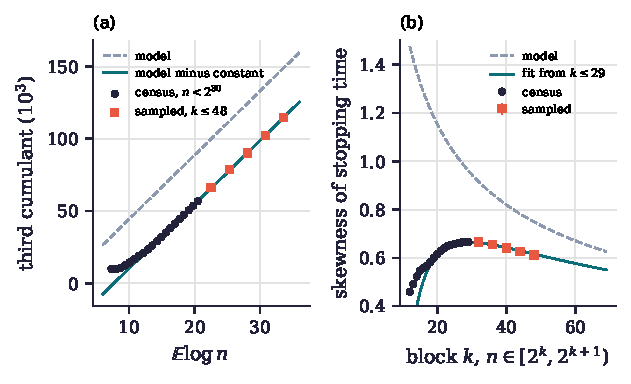
\includegraphics[width=\textwidth]{figures/ch16_o4.pdf}
\caption{The third cumulant of stopping times. (a) The third cumulant against
$\E\log n$: the census (dots), sampled blocks up to $k=48$ (squares), the
model line $A_3\,\E\log n$ (dashed) and the fit $a_3\,\E\log n-D_3$ (solid).
(b) Skewness: census, sampled blocks with two standard errors, the
prediction of the fit from $k\le29$, and the uncorrected model.}
\label{fig:ch16:o4}
\end{figure}

The variances agree to within $0.2$ percent, the third cumulants to within
$0.8$ percent, and the skewness to within two standard errors at every block,
while the uncorrected model is off by between $0.14$ and $0.25$. The skewness
peaks near $k=30$ and falls, as predicted: $0.640$ at $n\approx2^{40}$, a value
the model reaches only near $2^{66}$. Extrapolating, the skewness should be
$0.577$ at $2^{60}$ and $0.478$ at $2^{100}$, against model values $0.671$ and
$0.521$.

\paragraph{Status of O4.} The third cumulant is explained in the same sense as
the variance: the Bernoulli model is right about the slopes of the first three
cumulants to within a fraction of a percent, and the deficits behave as constants
contributed mostly by the finite system at the bottom of the orbit. The prediction
has been confirmed out of sample. What remains is a proof that the deficits
are bounded, which would require controlling the passage of the orbit from
the Terras horizon to the bottom, and that is the divergence half in
miniature. This also completes project P4 to the extent memory allows: the
sampled cumulants to $n\approx2^{49}$ show no departure from the fitted
constants.

\section{The exact convex rate of Switching MM}\label{sec:ch16:p11}

\Cref{conj:ch7b:tight} gave the worst case of $\smmdet$ on smooth convex
functions as $LR^2/((4+2\beta)N+2)$ for even $N$ and $\beta\le\beta_2$. We now
have a conjectured closed form for every $\beta<1$, and a proof for $N=2$ and $4$ on ranges of $\beta$ that contain the Collatz value.

\subsection{Two branches}

Write $D_N=(4+2\beta)N+2$ and $D'_N=4N-2+2(N-2)\beta$. The second quantity is
the same expression for the schedule that remains after the first long step:
$N-1$ steps, of which $N/2$ are unit steps and $N/2-1$ are long.

\begin{conjecture}[The exact convex rate of Switching MM, both branches]\label{conj:ch16:full}
For every even $N\ge2$ and every $0\le\beta<1$, the worst case of $\smmdet$ over
convex $L$ smooth functions with $\|x_0-x_*\|\le R$ is
\[
  \sup\bigl(f(x_N)-f_*\bigr)=LR^2\max\Bigl\{\frac1{D_N},\ \frac{\beta^2}{D'_N}\Bigr\}.
\]
The two branches cross at
\[
  \beta_N=\frac{\sqrt{9N^2-2N+1}-N-1}{2N},
\]
the positive root of $N\beta^2+(N+1)\beta-(2N-1)=0$, so that the main branch is
exact for all even $N$ exactly when $\beta\le\beta_2=(\sqrt{33}-3)/4=0.68614$.
\end{conjecture}

The crossing equation $\beta^2D_N=D'_N$ is the cubic
$2N\beta^3+(4N+2)\beta^2-2(N-2)\beta-(4N-2)=0$, which factors as
$(\beta+1)\bigl(2N\beta^2+(2N+2)\beta-(4N-2)\bigr)=0$; for $N=2$ it is the cubic
$2\beta^3+5\beta^2-3=(\beta+1)(2\beta^2+3\beta-3)$ of \cref{chap:threepoint}. The
thresholds are $\beta_2=0.6861$, $\beta_4=0.8381$, $\beta_6=0.8910$,
$\beta_8=0.9178$, $\beta_{10}=0.9341$, and $\beta_N\to1$. They agree with the
bisection values of \cref{chap:threepoint} to every digit computed, and
performance estimation agrees with the two branch formula to a relative error
below $2\times10^{-7}$ at $N=2,4,6,8,10$ and six values of $\beta$ on both sides
of each threshold, up to $\beta=0.99$ (script \texttt{ch16\_fullconj.py},
\cref{fig:ch16:smm}(a)).

\subsection{The lower bounds are attained by explicit functions}

\begin{proposition}[Two worst functions]\label{prop:ch16:lower}
For every even $N$ and $0\le\beta<1$ the supremum in \cref{conj:ch16:full} satisfies
\[
  \sup\bigl(f(x_N)-f_*\bigr)\ \ge\ LR^2\max\Bigl\{\frac1{D_N},\ \frac{\beta^2}{D'_N}\Bigr\}.
\]
\end{proposition}

\begin{proof}
Work in one dimension with $x_*=0$, $x_0=R$, and write $s_j\in\{1+\beta,1\}$ for the
step multipliers, so that a step from a point where the derivative is $c$
moves by $s_jc/L$.

For the first branch take the Huber function $f(x)=c|x|-c^2/(2L)$ for
$|x|\ge c/L$ and $f(x)=Lx^2/2$ otherwise, which is convex and $L$ smooth. As long
as the iterates stay in $x\ge c/L$ the derivative is $c$, so
$x_N=R-(W/2)c/L$ with $W=2\sum_js_j=(2+\beta)N$, and
$f(x_N)-f_*=cx_N-c^2/(2L)=cR-(W+1)c^2/(2L)$. The choice $c=LR/(W+1)$ gives
$LR^2/(2W+2)=LR^2/D_N$, and then $x_N=R(W+2)/(2(W+1))\ge c/L$, so every iterate
did stay in the linear region.

For the second branch take $f(x)=Lx^2/2$ for $x\ge-c/L$ and $f(x)=c|x|-c^2/(2L)$
for $x<-c/L$, again convex and $L$ smooth. The first step, of multiplier
$1+\beta$, starts in the quadratic region and lands at $x_1=R-(1+\beta)R=-\beta R$.
If $\beta R\ge c/L$ the remaining $N-1$ steps run in the linear region, and the
same computation with $R$ replaced by $\beta R$ and $W$ by
$W'=2\sum_{j\ge1}s_j=2N-2+(N-2)\beta$ gives $L\beta^2R^2/(2W'+2)=L\beta^2R^2/D'_N$, with
$c=L\beta R/(W'+1)\le L\beta R$ as required.
\end{proof}

The second function makes the meaning of the overshoot branch plain. A long
step on the quadratic part carries the iterate past the minimizer by a
fraction $\beta$ of the distance, and from there the remaining steps face the
method's own worst case, from distance $\beta R$. For small $\beta$ the overshoot is
harmless; beyond $\beta_N$ it is the worst thing that can happen.

\subsection{An explicit certificate}

The upper bound is the hard direction. Performance estimation solved with only
the inequalities between consecutive iterates and between each iterate and the
minimizer, the structure of the proof of Drori and Teboulle for gradient
descent, gives the same value as the full program (script
\texttt{ch16\_pep\_sparse.py}), so a certificate of that shape exists. Its
multipliers can be read off and have a closed form.

\begin{theorem}[An exact rate for two and four steps]\label{thm:ch16:cert}
Let $s_k=1+\beta$ for even $k$ and $s_k=1$ for odd $k$, let $x_{k+1}=x_k-(s_k/L)\nabla f(x_k)$ for $0\le k<N$ (for odd $k$ the point $x_k$ is the intermediate point $y$ of \cref{chap:threepoint}, and $x_N$ is the $N$th iterate of \smmdet), $W_k=2(s_0+\dots+s_k)$, and
\begin{gather*}
  \lambda_k=\frac{W_k}{D_N-W_k+2\beta\,[k\text{ even}]},\\
  \mu_0=\lambda_0,\qquad\mu_k=\lambda_k-\lambda_{k-1}\ (0<k<N),\qquad\mu_N=1-\lambda_{N-1}.
\end{gather*}
Multiply the interpolation inequality between iterates $k$ and $k+1$ by
$\lambda_k$ and the one between the minimizer and iterate $k$ by $\mu_k$, and sum.
The result is $f(x_N)-f_*\le LR^2/D_N-q$, where $q$ is a quadratic form in
$x_0-x_*$ and the gradients, and $q\ge0$ holds identically when
\begin{gather*}
  N=2\ \text{and}\ 0\le\beta\le b_2=0.64461,\qquad\text{or}\\
  N=4\ \text{and}\ 0\le\beta\le b_4=0.70438,
\end{gather*}
where $b_2$ and $b_4$ are the positive roots of $2\beta^4+11\beta^3+17\beta^2+\beta-11$
and $4\beta^4+21\beta^3+31\beta^2-\beta-23$. In these ranges, which contain the
Collatz value, \cref{conj:ch16:full} holds.
\end{theorem}

\begin{proof}
The multipliers are positive and increasing in $k$, since $W_k$ increases and the
denominator decreases, by $2$ from an odd $k-1$ to an even $k$ and by $2+2\beta$ from an
even $k-1$ to an odd $k$, and $\lambda_{N-1}=(2+\beta)N/((2+\beta)N+2)<1$, so all $\lambda_k$ and $\mu_k$ are nonnegative and $\sum_k\mu_k=1$. With these
weights the function values telescope to $f(x_N)-f_*$. The remaining quadratic
form has a matrix $S(\beta)$ of size $N+2$ in the basis $x_0-x_*,\nabla f(x_0),\dots,\nabla f(x_N)$,
computed symbolically in $\beta$ (script \texttt{ch16\_certificate.py}). It is
singular (its determinant vanishes identically), so it is positive semidefinite
if its leading principal minors of orders $1$ to $N+1$ are positive, since then its leading block of order $N+1$ is positive definite and the Schur complement of that block, a positive multiple of the determinant, is zero. For
$N=2$ these are, up to positive factors, $1$, $-(2\beta^2+3\beta-3)$ and
$-(2\beta^4+11\beta^3+17\beta^2+\beta-11)$, all positive on $[0,b_2)$, and $S(b_2)$ is positive semidefinite by continuity. For $N=4$ they
are, up to positive factors, $1$, $-(4\beta^2+5\beta-7)$, $-p(\beta)$,
$p(\beta)\,r(\beta)$ and $p(\beta)\,t(\beta)$, where $p=4\beta^4+21\beta^3+31\beta^2-\beta-23$,
$r=9\beta^4+42\beta^3+31\beta^2-84\beta-99$ and
$t=36\beta^6+312\beta^5+964\beta^4+1016\beta^3-722\beta^2-2280\beta-1287$; on $[0,b_4)$ the
polynomials $p$, $r$ and $t$ are all negative, so every minor is positive, and $S(b_4)$ is positive semidefinite by continuity.
Combined with \cref{prop:ch16:lower}, the bound is attained.
\end{proof}

Two features of the minors are worth recording. The second leading minor is
positive exactly below the true threshold: its factor $2\beta^2+3\beta-3$ for
$N=2$ and $4\beta^2+5\beta-7$ for $N=4$ is the crossing quadratic
$N\beta^2+(N+1)\beta-(2N-1)$. So the threshold of the conjecture is visible in the
certificate. The higher minors fail earlier, at $b_N<\beta_N$, which means that
these particular multipliers are optimal only in the lower part of the range
and a different certificate is needed near the threshold. Numerically the same
closed form multipliers give a positive semidefinite $S(\beta)$ for every even
$N\le20$ when $\beta$ is below a value that increases with $N$, from $0.6446$ at
$N=2$ to $0.7559$ at $N=20$, so the theorem very probably extends to all even
$N$ for $\beta\le b_2$, which includes $\beta=\lt-1$.

\paragraph{Status of P11.} The conjecture is now complete in closed form for
every $\beta<1$, both branches have rigorous lower bounds, and the upper bound is
proved for $N=2$ and $4$ on ranges containing the Collatz value. A proof for all
even $N$ along the lines of Drori and Teboulle, with the multipliers of
\cref{thm:ch16:cert}, needs the positivity of $S(\beta)$ in general, and a second
family of multipliers is needed between $b_N$ and $\beta_N$.

\section{Noise floors beyond quadratics}\label{sec:ch16:s2}

Problem S2 asks whether the noise bound $5/3$ of \cref{prop:ch7:bound} survives
beyond the quadratic model with isotropic noise, and project P5 asks for a test
on a real stochastic problem. We give a small extension and a test.

\begin{proposition}[Correlated noise]\label{prop:ch16:correlated}
On the quadratic of \cref{sec:ch7:model}, let the noise of the oracle have an
arbitrary covariance $Q$ instead of $\sigma^2I$, still independent from call to
call. Then for every step $\alpha\le1/L$ and every $0\le\beta<1$ the stationary excess loss
of $\smmdet$ is at most $5/3$ times that of gradient descent with the same step.
\end{proposition}

\begin{proof}
In the eigenbasis of $A$ all the methods act separately on each coordinate, so
the stationary covariance $C$ of the error satisfies
$\E[f-f_*]=\half\sum_i\lambda_iC_{ii}$, and $C_{ii}$ depends on the noise only through
the variance $Q_{ii}$ of its $i$th coordinate, linearly. By \cref{thm:smmvar}
applied to each coordinate, $C_{ii}^{\mathrm{SMM}}=r(a_i)\,C_{ii}^{\mathrm{GD}}$ with
$r\le5/3$ by \cref{prop:ch7:bound} and \cref{prop:ch7:uniform}. The ratio of
excess losses is therefore a weighted average of the $r(a_i)$, with nonnegative
weights $\lambda_iC_{ii}^{\mathrm{GD}}$.
\end{proof}

The correlations between coordinates, which make minibatch noise far from
isotropic, therefore do not matter on a quadratic. To see what the
nonlinearity does, we took the $\ell_2$ regularized multinomial logistic
regression on the digits data of scikit learn: $1797$ images, $64$ pixels and a
bias, ten classes, $650$ parameters, $\lambda=0.01$, so that $L=0.929$, $\mu=0.010$
and $\kappa=93$ at the minimizer (script \texttt{ch16\_s2\_softmax.py}). The linear
theory predicts the noise floor of each method from the Hessian $H$ at the
minimizer and the covariance $S$ of per sample gradients there, by solving the
discrete Lyapunov equation of the linearized dynamics with noise covariance
$S/b$ for minibatches of size $b$; for Switching MM the two step map is used.
The simulation runs each method on the true loss, from the minimizer, with step
$1/L$, for $20\,000$ iterations after a burn in, over six seeds.

\begin{table}[t]
\centering\small
\setlength{\tabcolsep}{4pt}
\caption{Noise floors $\E[f-f_*]$ on the digits problem, relative to gradient
descent, from the linear theory and from simulation, for minibatches of $16$
and $64$. Gradient descent itself: predicted $0.0660$ and $0.0165$, simulated
$0.0809$ and $0.0173$.}
\label{tab:ch16:s2}
\begin{tabular}{@{}lrrrr@{}}
\toprule
 & \multicolumn{2}{c}{$b=16$} & \multicolumn{2}{c}{$b=64$} \\
\cmidrule(lr){2-3}\cmidrule(l){4-5}
method & theory & simulation & theory & simulation \\
\midrule
Switching MM, $\beta=0.585$ & $1.094$ & $1.166$ & $1.094$ & $1.076$ \\
Nesterov, $\beta=0.585$ & $1.281$ & $2.049$ & $1.281$ & $1.428$ \\
Nesterov, $\beta=0.9$ & $2.198$ & $6.306$ & $2.198$ & $2.875$ \\
heavy ball, $\beta=0.9$ & $7.959$ & $21.77$ & $7.959$ & $10.60$ \\
\bottomrule
\end{tabular}
\end{table}

\Cref{tab:ch16:s2} and \cref{fig:ch16:smm}(b) give the result. At the
moderate noise level $b=64$ the linear theory predicts the absolute floor of
gradient descent to within five percent and that of Switching MM to within
three. At the heavy noise level $b=16$ the iterates wander far enough from the
minimizer for the curvature to change, every floor rises above the linear
prediction, and the rise is much larger for the momentum methods: every step
Nesterov at $\beta=0.9$ is six times worse than gradient descent instead of the
predicted two, and heavy ball twenty two times worse instead of eight.
Switching MM stays within $17$ percent of gradient descent at both noise
levels. The bound $5/3$ holds with room to spare on this nonquadratic problem,
and the nonlinearity widens the advantage of parity switching over every step
momentum rather than narrowing it.

\begin{figure}[t]
\centering
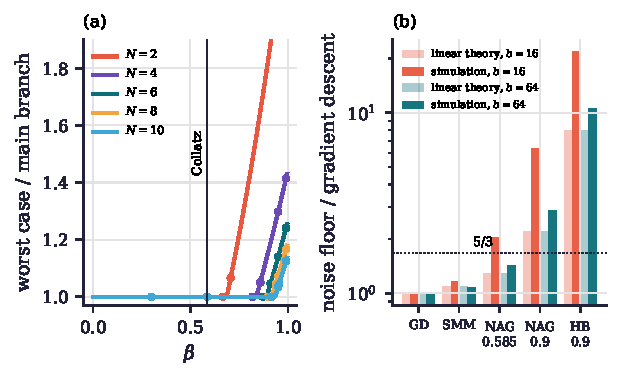
\includegraphics[width=\textwidth]{figures/ch16_smm.pdf}
\caption{(a) The worst case of Switching MM on smooth convex functions divided
by the main branch $LR^2/D_N$, from \cref{conj:ch16:full} (lines) and from
performance estimation (dots), for $N=2,\dots,10$. The overshoot branch takes over
at $\beta_N$. (b) Noise floors on the digits problem relative to gradient
descent: linear theory (pale) and simulation (solid) for minibatches of $16$
and $64$, with the bound $5/3$ dotted.}
\label{fig:ch16:smm}
\end{figure}

\paragraph{Status of S2 and P5.} Correlated noise is settled on quadratics.
The nonquadratic case remains open as a theorem, but on a real problem with
genuine minibatch noise the bound holds and the linear theory is accurate at
moderate noise. A test on deep networks, where the Hessian is not positive
definite, is the natural next step.

\section{Erd\H{o}s 125 to \texorpdfstring{$4^{17}$}{4 to the 17}}\label{sec:ch16:p7}

\Cref{sec:ch8:erdos} computed the density of $A+B$ exactly up to $4^{13}$, where
$A$ and $B$ are the integers whose base $3$ and base $4$ digits lie in $\{0,1\}$.
With a bit array and compiled loops (script \texttt{ch16\_erdos125.py}) the same
exact computation reaches $4^{17}=17\,179\,869\,184$, a range $256$ times
larger, in eleven minutes. It reproduces every value of
\cref{tab:ch8:erdos}. The new densities are $0.8760$, $0.7855$, $0.7936$ and
$0.8453$ at $4^{14}$ to $4^{17}$, and the minimum over $[10^4,4^{17}]$ is still
$0.763392$ at $3^{15}-1$.

The minima sit just below powers of $3$, and the computation shows what
controls their depth. Write $f_m$ for the fractional part of $m\log_43$, so
that $3^m=4^{\lfloor m\log_43\rfloor}\cdot4^{f_m}$. \Cref{tab:ch16:erdos} lists the
density at $3^m-1$ for $10\le m\le21$ against $f_m$.

\begin{table}[t]
\centering\small
\caption{Density of $A+B$ in $[0,3^m-1]$ against the fractional part $f_m$ of
$m\log_43$, sorted by $f_m$. Pairs of rows with close $f_m$ come from different
scales and have close densities.}
\label{tab:ch16:erdos}
\begin{tabular}{@{}rll@{\qquad}rll@{}}
\toprule
$m$ & $f_m$ & density & $m$ & $f_m$ & density \\
\midrule
$19$ & $0.057$ & $0.7924$ & $21$ & $0.642$ & $0.8312$ \\
$14$ & $0.095$ & $0.8147$ & $16$ & $0.680$ & $0.8312$ \\
$18$ & $0.265$ & $0.8813$ & $11$ & $0.717$ & $0.8372$ \\
$13$ & $0.302$ & $0.8742$ & $20$ & $0.850$ & $0.7679$ \\
$17$ & $0.472$ & $0.8590$ & $15$ & $0.887$ & $0.7634$ \\
$12$ & $0.510$ & $0.8583$ & $10$ & $0.925$ & $0.7785$ \\
\bottomrule
\end{tabular}
\end{table}

To within about $0.015$, the density at $3^m-1$ is a function of $f_m$ alone,
across a range of scales from $3^{10}$ to $3^{21}$
(\cref{fig:ch16:erdos}(a)). It is largest near $f_m\approx0.3$ and smallest near
$f_m\approx0.88$, where a power of $3$ lies a little below a power of $4$, at a
ratio $4^{f_m-1}\approx0.85$, and the gaps of $A$ and $B$ align, as described in
\cref{sec:ch8:erdos}. There is no visible drift with scale at fixed $f_m$: the pairs
$(15,20)$, $(12,17)$, $(13,18)$ and $(11,16,21)$ agree to within $0.007$. The
theorem of AlphaProof Nexus that the lower density is zero must therefore act
through approximations far better than any in range, such as
$3^{53}\approx4^{42}$ with $f_{53}=0.0015$, consistent with the windows its proof
uses.

\paragraph{Status of P7.} The computation is extended to $4^{17}$; the depth of
the minima is controlled by $f_m$ with no drift at fixed $f_m$ up to $3^{21}$. A
heuristic for the limiting profile as a function of $f_m$, and for the scale at
which it must begin to fall, would make the picture quantitative.

\section{Single orbits from \texorpdfstring{$2^{300000}$}{2 to the 300000}}\label{sec:ch16:p3}

Project P3 asks whether single orbits from much larger starting values show
any departure from independent sampling. We followed four Syracuse orbits
from random odd integers near $2^{100000}$, of about $241\,000$ steps each, and
one from near $2^{300000}$, of $723\,876$ steps, thirty times the scale of
\cref{sec:ch9:single} (script \texttt{ch16\_p3\_orbits.py}). Along each orbit we
tested four things, each against a null calibrated to the orbit's length.

\begin{itemize}[leftmargin=1.5em]
\item Residues modulo $3^a$ for $a=5,\dots,8$: the total variation distance of the
  empirical law from the stationary law $\pi_a$ of the induced chain is between
  $0.89$ and $1.06$ times the mean distance for independent samples from $\pi_a$
  of the same length (\cref{fig:ch16:erdos}(b)).
\item Consecutive residues modulo $3^4$: a $\chi^2$ statistic of the transition
  counts against the induced chain, restricted to cells with expected count at
  least $5$, lies within $1.7$ standard deviations of its distribution under
  the chain itself, simulated for the same length, on all five orbits.
\item Halving exponents: the means are $1.9992$, $1.9989$, $2.0034$, $2.0005$ and
  $1.9994$, against $2$, with $z$ scores between $-0.4$ and $1.2$; the
  autocorrelations at lags $1$ to $5$ are all below $0.0031$ in absolute value,
  against a standard error of $0.0020$, and $0.0012$ for the longest orbit.
\item Low binary digits modulo $2^{12}$: $\chi^2$ tests against the uniform law on
  odd classes give $p$ values $0.88$, $0.77$, $0.03$, $0.99$ and $0.05$, as
  expected of five independent tests.
\end{itemize}

\paragraph{Status of P3.} At thirty times the earlier scale, with moduli up to
$3^8$ and with joint and serial statistics, no statistic of a single orbit
departs from independent sampling. The evidence for trajectory mixing (O2)
is correspondingly stronger; the proof is as far away as before.

\begin{figure}[t]
\centering
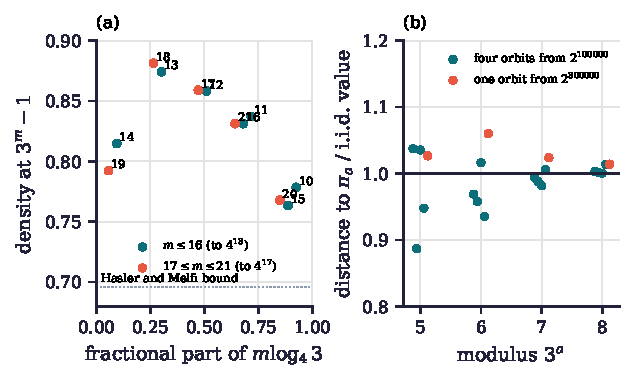
\includegraphics[width=\textwidth]{figures/ch16_erdos.pdf}
\caption{(a) Erd\H{o}s $125$: the density of $A+B$ at $3^m-1$ against the
fractional part of $m\log_43$, for $10\le m\le21$, labelled by $m$; the depth of
the minima depends on $f_m$ and not on the scale. (b) Single orbits: total
variation distance of the residues modulo $3^a$ from $\pi_a$, divided by its
mean under independent sampling, for four orbits from $2^{100000}$ and one from
$2^{300000}$.}
\label{fig:ch16:erdos}
\end{figure}

\section{Where the problems stand}\label{sec:ch16:status}

\Cref{tab:ch16:status} records the status of every problem of
\cref{chap:open} after this chapter and the rest of the book.

\begin{table}[t]
\centering\small
\setlength{\tabcolsep}{3pt}
\caption{Status of the open problems and projects.}
\label{tab:ch16:status}
\begin{tabular}{@{}l>{\raggedright\arraybackslash}p{0.80\textwidth}@{}}
\toprule
O1, O2 & open; P3 strengthens the evidence for O2 \\
O3, O3$'$ & open; \cref{chap:mmcollatz} rules out bounded depth \\
O4 & third cumulant explained and predicted out of sample (\cref{sec:ch16:o4}); boundedness of the deficits open \\
O5 & settled by \cref{prop:uimartingale}; no separate open problem \\
C1, C2, C3 & open \\
B1, B2, B3 & open \\
S1 & settled for the distance by \cref{thm:ch5b:rate}; the function gap for $\kappa<(1+\beta)/(1-\beta)$ open \\
S2 & open; on quadratics extended to any noise covariance (\cref{prop:ch16:correlated}); supported on a real problem \\
S3 & settled on quadratics by \cref{prop:ch7:pareto}; the choice of scale without $\mu$ open \\
S4 & open \\
P1, P2 & open \\
P3 & done to $2^{300000}$, no departure found \\
P4 & done to $n\approx2^{49}$ by sampling, consistent with constant deficits \\
P5 & done on one real problem; deep networks open \\
P6 & settled in the slow mode by \cref{thm:ch7:gainweight} \\
P7 & extended to $4^{17}$; minima controlled by $f_m$ \\
P8, P9, P10 & open \\
P11 & complete conjecture, both lower bounds, proof for $N=2$, $\beta\le0.6446$, and $N=4$, $\beta\le0.7043$ (\cref{sec:ch16:p11}) \\
\bottomrule
\end{tabular}
\end{table}

\section*{Notes}

The cumulants of first passage times of random walks, and the absence of a
third cumulant correction for symmetric steps, follow from Wald's identities
and are in Feller~\cite{feller1971} and Gut~\cite{gut1988}. The structure of the
certificate in \cref{thm:ch16:cert} follows Drori and Teboulle~\cite{drori2014};
the interpolation conditions are those of Taylor, Hendrickx and
Glineur~\cite{taylor2017}, and the Huber function is the classical worst case
for gradient descent. The digits data are distributed with scikit learn. The
Erd\H{o}s $125$ problem and its solution are discussed in \cref{sec:ch8:erdos},
with references there. All results in this chapter are new; the scripts are
listed in \cref{app:code}.

\section*{Exercises}

\begin{exercise}
For a random walk with increments $\pm\half\log3$ and drift $\mu<0$, use Wald's
identities to show that the third cumulant of the first passage time below
$-u$ grows like $3\sigma^4u/|\mu|^5$, and explain why a skewed step distribution
would add a term proportional to $\kappa_3$ of the step.
\end{exercise}

\begin{exercise}
Verify the factorization
$2N\beta^3+(4N+2)\beta^2-2(N-2)\beta-(4N-2)=(\beta+1)(2N\beta^2+(2N+2)\beta-(4N-2))$ and
show that $\beta_N\to1$ like $1-2/(3N)$.
\end{exercise}

\begin{exercise}
For the gradient method with an arbitrary step schedule $s_0,\dots,s_{N-1}$ in $(0,2)$, repeat the first half of the proof of
\cref{prop:ch16:lower} and show that the Huber function gives the lower bound $LR^2/(2W+2)$ with
$W=2\sum_js_j$. Check that for constant steps $s_j=1$ this is the bound
$LR^2/(4N+2)$ of Drori and Teboulle.
\end{exercise}

\begin{exercise}
Show that in the eigenbasis of $A$ the stationary covariance of gradient
descent with step $\alpha$ on the quadratic of \cref{prop:ch16:correlated} has
entries
\[
  C_{ij}=\frac{\alpha^2Q_{ij}}{1-(1-a_i)(1-a_j)},\qquad a_i=\alpha\lambda_i,
\]
and that only its diagonal enters the excess loss.
\end{exercise}

\chapter{Contributions and a Computational Road Map}\label{chap:synthesis}

This book does not prove the Collatz conjecture. It does change what is known
about the problem, in three ways that are easy to lose among the details of
seventeen chapters: it adds a set of results, exact and quantitative, about the
map and about the optimizer the map suggests; it proves that a long list of
natural strategies cannot work, which narrows the space in which a proof can
live; and it corrects several claims, including some of our own. This chapter
collects all three in one place, with pointers to where each is proved and an
honest statement of what is new. It then uses them to lay out a computational
path to a solution: a staged programme in which every stage proves something
definite, the points where mathematics rather than computation must supply
the next step are marked, and the one route that could settle the whole
conjecture by finite computation is identified.

\section{The problem as the book leaves it}\label{sec:ch10d:state}

The conjecture is the conjunction of two statements that need different tools
(\cref{chap:path}).

The divergence half says that no orbit is unbounded. By the Ces\`aro identity\index{Cesaro identity@Ces\`aro identity}
(\cref{prop:cesaro}) it is equivalent to a law of large numbers along every
single orbit: the running mean $\bar k_N$ of the halving exponents
$\vt(3y_i+1)$ has lower limit strictly greater than $\lt\approx1.585$
(\cref{conj:cesaro}). The Bernoulli model predicts that the mean is $2$, and
Tao's theorem (\cref{thm:ch1:tao}) proves a version of this for almost every
starting value in logarithmic density, but nothing is known about any
particular orbit.

The cycle half says that the only cycle is $1\to2\to1$. By the periodic point formula
(\cref{cor:ch2:cycle} and the rational cycles of \cref{chap:cycles}) a cycle with $m$ odd steps among $k$ steps exists if and only
if some binary word $w$ of length $k$ with $m$ ones has $2^k-3^m$ dividing the
number $c_k(w)$ with a positive quotient. This is a divisibility question
about sums of terms $3^j2^i$, and it has nothing to do with averages.

The state of the art on each half, as of this writing, is the following.
Every starting value up to $2^{71}$ reaches $1$~\cite{barina2025}. Every
nontrivial cycle has at least $137\,528\,045\,312$ odd elements, by Hercher's
sharper accounting at that range; the exact certificate of \cref{thm:cycles} gives $72\,057\,431\,991$. No cycle has $m\le91$
ascending runs (Hercher, extending Simons and de Weger). At least $x^{0.84}$
integers up to $x$ reach $1$ (Krasikov and Lagarias), and by unrefereed preprints of 2026 by Mazur and by Lau, whose proofs the book does not check, a positive proportion do (\cref{chap:backward}). Almost every orbit attains
almost bounded values (Tao). The two halves are therefore both open, and in
both the obstruction is the same: every known method sees either an ensemble of
starting values or a bounded number of binary digits of one starting value, and the
conjecture is about every digit of every positive integer.

\section{What the book contributes}\label{sec:ch10d:contrib}

\Cref{tab:ch10d:contrib} lists the main results. The status column uses five
labels. \emph{New} means the result first appears in this book or in the
authors' earlier paper on Collatz dynamics. \emph{New proof} means the fact is
classical and the book gives a short, self contained proof in the form it needs.
\emph{Computed} means new exact numbers produced by the scripts of
\cref{app:code}. \emph{Corrected} means the book replaces an earlier claim,
ours or another's, by a correct one. \emph{Conditional} means the result assumes a statement the book does not prove, named in the cell. The Notes of each chapter give the
attributions in full; where a result builds on a named predecessor the table
says so.

\needspace{14\baselineskip}
{\small
\setlength{\tabcolsep}{3pt}
\begin{longtable}{@{}p{0.47\textwidth}>{\raggedright\arraybackslash}p{0.25\textwidth}>{\raggedright\arraybackslash}p{0.22\textwidth}@{}}
\caption{The main results of the book, with where they are proved and their
status.}\label{tab:ch10d:contrib}\\
\toprule
Result & Where & Status \\
\midrule
\endfirsthead
\toprule
Result & Where & Status \\
\midrule
\endhead
\bottomrule
\endfoot
\multicolumn{3}{@{}l}{\itshape Exact structure of the map}\\*
\addlinespace[2pt]
The halving exponent $\vt(3n+1)$ is exactly Geometric$(\half)$ on residue classes, and the Syracuse drift is exact & \cref{prop:geom}, \cref{cor:ch2:drift} & exact form of a classical heuristic \\
Martingale duality: $x_n$ a martingale, $\log x_n$ a strict supermartingale, the gap Jensen's & \cref{thm:martingale} & parts classical (Crandall; Lagarias and Weiss) \\
Parity autocorrelation $\rho(h)=(-\tfrac12)^h$ and the long run variance factor & \cref{thm:autocorr}, \cref{cor:longrun} & new \\
Exact stopping counts by a two term recursion & \cref{prop:ch2:dp} & Terras's recursion \\
Pathwise decomposition; the ten percent variance deficit of the stopping time sits at the bottom of the orbit (census to $2^{30}$) & \cref{prop:ch3:pathwise}, \cref{sec:ch3:missing} & computed; boundedness open (\cref{prob:ch11:o4}) \\
The third cumulant deficit behaves as an additive constant in the final descent; skewness predicted out of sample to $2^{49}$ & \cref{prop:ch16:deficit}, \cref{tab:ch16:o4} & computed; boundedness open (\cref{prob:ch11:o4}) \\
Uniform integrability fails, so optional stopping cannot be used & \cref{prop:uimartingale} & new proof \\
\addlinespace[4pt]
\multicolumn{3}{@{}l}{\itshape Cycles and continued fractions}\\*
\addlinespace[2pt]
Mediant lemma for the one sided distances $\lceil r\lt\rceil-r\lt$ & \cref{lem:ch8:mediant} & new proof (Hercher's Lemma 22) \\
Every nontrivial cycle has $r\ge72\,057\,431\,991$ odd elements, with an exact integer certificate of $44$ rungs & \cref{thm:cycles}, \cref{sec:ch8:certificate} & method Eliahou's, bound Hercher and Puchert's; certificate new \\
Verification thresholds: where extending the verified range moves the bound & \cref{tab:ch8:thresholds} & computed \\
Diophantine insufficiency: no irrationality measure plus verification excludes all cycles & \cref{prop:ch8:insufficient} & new form of a point of Halbeisen and Hungerb\"uhler; corrects our paper \\
Window lemma: an arithmetic margin of order $m/3$ would exclude all cycles & \cref{lem:ch8:window}, \cref{cor:ch8:window} & new \\
Machine checked statements in Lean & \cref{sec:ch8:lean} & new \\
Erd\H{o}s $125$ density exact to $4^{17}$; depth of minima a function of the fractional part of $m\log_43$ & \cref{sec:ch16:p7} & computed \\
\addlinespace[4pt]
\multicolumn{3}{@{}l}{\itshape Divergence, counting and residues}\\*
\addlinespace[2pt]
Ces\`aro identity: divergence is equivalent to a running mean at most $\lt$ & \cref{prop:cesaro} & new formulation \\
Model chain modulo $3^a$ exactly stationary after $a$ strides; the apparent spectral gap modulo $27$ is spurious & \cref{lem:ch9:mixing}, \cref{rem:ch9:oddreps} & restates an identity of Tao; computed \\
Certified exponents for the inverse tree, $x^{0.477}$ integers reach $1$ & \cref{thm:ch5b:exponent}, \cref{cor:ch5b:count} & new proof of a weaker classical bound \\
Residue certificates of every depth fail on a closed null set containing $-1$, $-5$, $-17$ & \cref{prop:ch10b:residue} & new statement \\
Residue sieve grows like $2^{0.95k}$, the exponent $H(1/\lt)$ & \cref{sec:ch10b:divergence} & computed \\
Bregman decomposition of orbits; uniform dissipation $c_*=D(7/9)$ per Syracuse step & \cref{prop:ch7b:bregman}, \cref{prop:ch7b:dissipation} & new \\
Given the positive density theorems and the verification to $2^{71}$, logarithmic density one of the orbits reaching $1$, and so a bounded form of Tao's theorem, implies the conjecture & \cref{prop:ch9b:bounded} & new; conditional on the unrefereed preprints of Mazur and Lau \\
Step counts of the positive density theorems below $3\cdot10^6$; the exact $3$ adic offset law to level $18$; the backward tree from $1$ below $2^{24}$ & \cref{sec:ch9b:steps}, \cref{sec:ch9b:offsets}, \cref{tab:ch9b:tree} & computed \\
\addlinespace[4pt]
\multicolumn{3}{@{}l}{\itshape Majorization pressed to its limit}\\*
\addlinespace[2pt]
The cycle inequality is the descent inequality of the multiplicative majorizer & \cref{prop:ch5c:cyclemm} & reformulation of the classical cycle identity \\
No potential $\log x+\varphi(x\bmod2^k)$ certifies descent, for any $k$ & \cref{thm:ch5c:residue} & new \\
Surplus along chains; the block map and its descent frequency & \cref{prop:ch5c:surplus}, \cref{prop:ch5c:block} & surplus new; block map from Terras and Steiner \\
Run length potentials $\log x+c\,\vt(x+1)$ fail, in the model, on more than $14.3$ percent of odd integers for every $c>\log(3/2)$ & \cref{prop:ch5c:runpot} & new \\
\addlinespace[4pt]
\multicolumn{3}{@{}l}{\itshape Simulation}\\*
\addlinespace[2pt]
Two horizons: level sets of $\tau$ are clopen, those of $\sigma_\infty$ have no $2$ adic description & \cref{prop:ch10b:horizons} & new \\
Perfect split sampling of the exceptional classes at any depth, $O(k)$ per draw & \cref{thm:ch10b:perfect} & new \\
Coalescence or independence for local moves in deep level sets & \cref{prop:ch10b:acceptance} & new \\
Slow integers below $2^B$ form a small number of trees of merged orbits & \cref{tab:ch10b:clusters}, \cref{tab:ch10b:trees} & computed \\
\addlinespace[4pt]
\multicolumn{3}{@{}l}{\itshape The optimizer}\\*
\addlinespace[2pt]
Two steps of Switching MM are gradient steps of sizes $\alpha$ and $(1+\beta)\alpha$ on quadratics & \cref{thm:smmquad} & new \\
Exact stationary variance; noise amplification below $5/3$ for every $\beta<1$ and every step & \cref{thm:smmvar}, \cref{prop:ch7:uniform} & new; corrects the halving heuristic \\
Gain weight theorem: no periodic schedule beats gradient descent's noise floor at matched speed & \cref{thm:ch7:gainweight}, \cref{cor:ch7:nobeat} & new \\
Exact joint spectral radius; every switching rule is stable if the transient bound conjecture holds & \cref{prop:ch5b:jsr}, \cref{cor:ch5b:anyswitch} & new; the second part conditional on \cref{conj:ch5b:transient} \\
Linear rate on smooth strongly convex functions, exact in the worst case & \cref{thm:ch5b:rate} & new \\
Rate and noise frontier for period two steps; multiplicative noise thresholds & \cref{prop:ch7:pareto}, \cref{prop:ch7:mult} & new \\
Convex rate of Switching MM by three point inequalities, a factor $1+\beta/2$ better than gradient descent when $1+\beta\le\varphi$ & \cref{thm:ch7b:smmrate} & new \\
Exact convex worst case of Switching MM: two branch formula, thresholds $\beta_N$, explicit worst functions, proof for $N=2$, $\beta\le0.6446$, and $N=4$, $\beta\le0.7043$ & \cref{conj:ch16:full}, \cref{thm:ch16:cert} & new; partly conjectured \\
Noise bound $5/3$ for any noise covariance on quadratics; tested on a real problem & \cref{prop:ch16:correlated}, \cref{sec:ch16:s2} & new \\
Acceleration by similar triangles survives every switching rule & \cref{prop:ch7b:switch} & new \\
\end{longtable}}

Three of these deserve a sentence each, because they change how one should
think about the problem rather than adding a fact to it.

The cycle certificate and the insufficiency proposition belong together. The
first shows that the classical route, verification combined with the
continued fraction of $\lt$, can be made exact and short: forty four rungs of a
ladder and one integer inequality per rung. The second shows that the same
route can never finish, since infinitely many cycle lengths survive every
verification range under every irrationality measure. The window lemma then
says exactly what extra arithmetic would finish it. Together they turn a vague
belief, that cycles are a Diophantine problem, into a precise statement of what
Diophantine approximation can and cannot contribute.

The residue theorem of \cref{chap:mmcollatz} and the residue certificate
proposition of \cref{chap:computation} say the same thing from two sides. A
potential, or a certificate, that reads $n$ through a bounded number of binary digits
applies equally to the $2$ adic integers, and on the $2$ adic integers the map
has the fixed point $-1$, the cycle $-5\to-7\to-10\to-5$ and a cycle of
eleven elements through $-17$. No such
argument can therefore succeed. This is the integrality principle of the next
section.

The perfect sampler and the tree decomposition give the computational side of
the problem a precise shape. Up to the bit length of the integers involved,
every exceptional class can be sampled exactly in polynomial time; beyond it, the
slow integers below $2^{26}$ form a small number of long orbits with their tributaries, and no
local move leaves one except rarely.

\section{The ledger of obstructions}\label{sec:ch10d:obstructions}

The book proves that a long list of strategies cannot work.
\Cref{tab:ch10d:obstructions} collects them. Each row names the approach, the
result that rules it out, and what survives the obstruction, which is often the
most useful information in the row.

\begin{table}[!htbp]
\centering\small
\setlength{\tabcolsep}{3pt}
\caption{Strategies the book rules out. The last column records what the
obstruction leaves open.}
\label{tab:ch10d:obstructions}
\begin{tabular}{@{}>{\raggedright\arraybackslash}p{0.33\textwidth}>{\raggedright\arraybackslash}p{0.24\textwidth}>{\raggedright\arraybackslash}p{0.37\textwidth}@{}}
\toprule
Approach & Ruled out by & What survives \\
\midrule
Monotone strong Lyapunov function over one stride & \cref{thm:nolyapunov} & descent on average only \\
Monotone certificate over any fixed horizon & \cref{cor:ch4:multistride} & a variable horizon, the stopping time \\
Linear and power majorizers & \cref{prop:mmfails}, \cref{prop:ch4:power} & the logarithmic potential \\
Potential $\log x+\varphi(x\bmod2^k)$ & \cref{thm:ch5c:residue} & potentials that read integrality \\
Block and run length potentials & \cref{prop:ch5c:runpot} & none at bounded depth \\
Residue certificates of any depth & \cref{prop:ch10b:residue} & a null set containing $-1,-5,-17$ \\
Optional stopping for the martingale & \cref{prop:uimartingale} & conditioning, which is circular \\
Ensemble mixing transferred to one orbit & \cref{sec:ch10:divergence} & Tao's logarithmic density; density one of reaching $1$, given the preprints (\cref{cor:ch9b:densityone}) \\
Numerical checks of the Ces\`aro criterion & \cref{rem:ch9:circular} & nothing; the check is automatic \\
Constrained switching certificates & \cref{sec:ch10b:guidance} & none; every word is realized \\
Verification plus Diophantine approximation & \cref{prop:ch8:insufficient} & an arithmetic margin of order $m/3$ \\
Modular sieve on $c_k(w)$ with small primes & \cref{sec:ch10b:cycles} & large prime factors of $2^k-3^m$ \\
Level set samplers on $\sigma_\infty$ beyond the bit length & \cref{prop:ch10b:acceptance} & exact sampling of $\tau$ \\
\bottomrule
\end{tabular}
\end{table}

The rows fall into two families, and seeing them as families is the main
lesson of the ledger.

The first family consists of arguments that use only a bounded number of binary
digits of the starting value: one stride, $J$ strides, a residue modulo $2^k$,
a block of trailing ones, a sieve to depth $k$, a bit flip move. Each of these
arguments applies without change to the $2$ adic integers, where the
conjecture is false.

\begin{remark}[The integrality principle]\label{rem:ch10d:integrality}
Let $\mathcal A$ be an argument whose every step is valid for the accelerated
map on $\Ztwo$, the ring of $2$ adic integers. Then $\mathcal A$ cannot prove
that every orbit of a positive integer reaches $1$, because its conclusion
would also hold for the orbit of $-1$, which is fixed. A proof of the
conjecture must therefore use, at some step, a property that distinguishes the
positive integers inside $\Ztwo$. The simplest such property is that a positive
integer has a terminating binary expansion with a leading digit $1$, while
$-1=\dots1111$ does not terminate. Every obstruction of the first family is an
instance of this remark, and \cref{prop:ch10b:residue} is its precise form
for residue arguments.
\end{remark}

The second family consists of arguments that average over starting values:
the martingale, mixing on residues, the spectral gap, the central limit
theorem for stopping times, the samplers. These see the integers only through
ensembles, and the conjecture is a statement about each orbit separately. The
Bernoulli model is excellent, predicting the stopping time slope to half a
percent and its variance to about ten percent, a deficit that the census of \cref{chap:stochastic} locates at the bottom of the orbit; but
no mechanism is known that transfers such statistics to a single trajectory.
The one transfer the book records goes through density: given the unrefereed positive density preprints, a set of starting values of upper density one whose orbits reach $1$ would force every orbit to reach $1$ (\cref{cor:ch9b:densityone}), and Tao's theorem misses this only because its bound must tend to infinity (\cref{prob:ch11:b1}).

A proof, then, must use the integrality of $n$, and, unless it goes through density one as in \cref{prop:ch9b:bounded}, it must do so orbit by orbit.
The computational path below is designed around exactly those two
requirements.

\subsection*{Corrections and pitfalls}

The book corrects four claims. The irrationality measure bound of our original
paper had the exponent $\nu-2$ where $\nu$ is right, so it was too strong by a factor $r^2$; the correct statement is
$M<r^\nu/(3c\log2)$, and the conclusion drawn from it is reversed, since it
shows that no measure suffices (\cref{rem:irrmeasure}, \cref{prop:ch8:insufficient}).
The record structure of the cycle bound, which we first presented as a
discovery, is classical (\cref{chap:cycles}, Notes). The noise heuristic of the
Switching MM study, that parity switching halves the amplification of
momentum, predicts the wrong limit; the exact variance is bounded by $5/3$ and
the heuristic is explained in \cref{rem:ch7:heuristic}. And the description
of the identity $\beta=1-\mu_\ast/L_\ast$ as a structural fact is withdrawn; it
is a definitional rewriting (\cref{rem:ch6:definitional}).

The book also records the arguments that look like progress and are not,
because a reader who meets them elsewhere should recognize them: the
bookkeeping of odd runs under the accelerated map (\cref{rem:ch2:pitfall},
\cref{rem:ch8:bookkeeping}), the logarithm squared and minus logarithm
majorizers (\cref{rem:ch4:logsqpitfall}, \cref{rem:ch4:minuslog}), mixing
levels in momentum arguments (\cref{rem:ch5:mixing}), the wrong null hypothesis
for residue tests (\cref{rem:ch9:null}), and the Ces\`aro check that every
terminating orbit passes automatically (\cref{rem:ch9:circular}).

\section{A computational path to a solution}\label{sec:ch10d:path}

A computation proves a universal statement only by producing a finite object,
a certificate, together with a small trusted program that checks it and a
theorem that the check implies the statement. The verified range $2^{71}$ is a
certificate for a finite statement; the $44$ rung ladder of
\cref{sec:ch8:certificate} is a certificate for the cycle bound. A computational
solution of the conjecture would be a certificate of the same kind for the
whole statement. The ledger of the previous section says what such a
certificate must look like: it must read the integrality of $n$, and it must
handle every orbit separately, with a horizon that varies with $n$. The path
below is organized around those constraints. It has a shared kernel and two
lanes (\cref{fig:ch10d:roadmap}), and it is arranged so that every stage
proves something definite whether or not the later stages succeed.

\begin{figure}[!htbp]
\centering
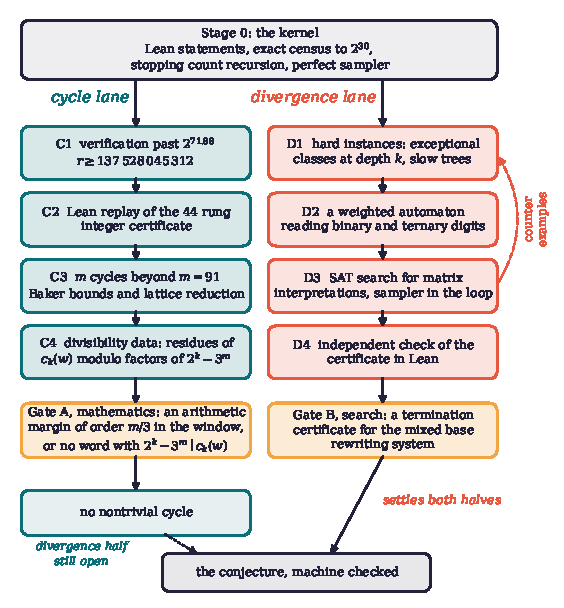
\includegraphics[width=\textwidth]{figures/ch10d_roadmap.pdf}
\caption{A computational road map. The kernel supplies exact tools shared by
both lanes. The cycle lane produces definite partial results at every stage
but needs a mathematical step at Gate A. The divergence lane is a search for a
single certificate; if Gate B is passed, the certificate settles both halves
at once. The dashed loop is the counterexample guided refinement of
\cref{sec:ch10d:lanes}.}
\label{fig:ch10d:roadmap}
\end{figure}

\subsection{Stage 0: the kernel}

The kernel is what the book already provides and what every later stage uses.
It has four parts. The Lean statements of \cref{sec:ch8:lean} fix the trusted
checker and the precise form of the conjecture, of descent and of the absence of nontrivial cycles. The exact census to $2^{30}$
(\cref{sec:ch3:missing}) supplies ground truth for every statistic of
stopping times. The stopping count recursion of \cref{prop:ch2:dp} gives the
exact volume $1-F(k)$ of the exceptional set at every depth in $O(k^2)$
operations. And the perfect sampler of \cref{thm:ch10b:perfect} draws a uniform
exceptional residue at depth $k$ in $O(k)$ operations. The last two together
mean that the hard part of the input space, the classes that have not yet
descended, is a computable and samplable object at every finite depth.

\subsection{The two lanes}\label{sec:ch10d:lanes}

\paragraph{The cycle lane.} Its stages are those of \cref{tab:ch10b:programme},
now ordered by what they buy.

C1 extends verification past $2^{71.884}$. By \cref{tab:ch8:thresholds} the
exact certificate of \cref{thm:cycles} then reaches $r\ge137\,528\,045\,312$ odd elements, the
record that Hercher's sharper accounting already gives at the verified range $2^{71}$; the next threshold is at $2^{75.433}$.
It costs less than twice the effort of the range $2^{71}$ and is pure
engineering. Every extension of the verified range also weakens what \cref{prob:ch11:b1} asks, since the constant $2^{71}$ of \cref{prop:ch9b:bounded} is the verified range.

C2 replays the $44$ rung certificate in Lean, turning
\cref{thm:cycles} into a machine checked theorem (project P1 of \cref{chap:open}).

C3 extends the exclusion of $m$ cycles beyond $m=91$. Each value of $m$ is a
finite computation, a lower bound for a linear form in logarithms followed by
lattice reduction, and each excluded $m$ is a theorem. The cost grows with $m$
and the method has no end point, so C3 produces results but cannot finish.

C4 gathers the data for Gate A. For each admissible shape $(m,k)$ near the rungs
of the ladder, factor $D=2^k-3^m$, and for each prime factor $p$ compute the
set of residues of $c_k(w)$ modulo $p$ over all words with $m$ ones, by the
recursion of \cref{sec:ch10b:cycles} in time proportional to $pkm$. With primes
below $3000$ this excludes only shapes with $m\le8$; the point of C4 is
different. It records, shape by shape, how close the words come to the
divisibility, and so produces the evidence on which a conjecture about the
numbers $c_k(w)$ can be formulated.

Gate A is mathematics. By \cref{cor:ch8:window} an arithmetic improvement of
the upper end of the window by a factor of order $m/3$ excludes all cycles; the
exploration of \cref{chap:cycles} shows that no argument from size alone can
provide it for balanced words. What is needed is a divisibility theorem: no
word $w$ with $m$ ones among $k$ letters has $2^k-3^m\mid c_k(w)$, apart from
the trivial cycle. Computation can find the right statement and test it on all
words up to a moderate length; it cannot supply the proof.

\paragraph{The divergence lane.} This lane is a search for a single
certificate, and if it succeeds it settles the whole conjecture, cycles
included. The reason is the theorem of Yolcu, Aaronson and Heule
(\cref{sec:ch10b:automated}): the Collatz map can be encoded as a string
rewriting system on a mixed binary and ternary representation whose
termination is \emph{equivalent} to the conjecture. A termination proof
excludes divergent orbits and nontrivial cycles alike. Their search found
proofs of nontrivial weakenings but not of the conjecture itself. The book
supplies four pieces of guidance that sharpen the search.

D1 builds the instances that a candidate certificate must survive. The perfect
sampler gives exact uniform draws from the exceptional classes at depth $k$, for
$k$ in the hundreds; the census gives every integer below $2^{30}$ with its
stopping time; and the tree decomposition of \cref{chap:samplers} gives the
slow integers below $2^{26}$ organized into trees of merged orbits, thirty four
of them above level $400$, each represented by the orbit at its root. These are the hardest instances in each sense: the
deepest residues, the slowest integers, and the representatives of
independent slow orbits.

D2 fixes the class of potentials. The ledger dictates three features. The
leading term must be logarithmic, since $x_n$ itself is a martingale and has no
drift (\cref{thm:martingale}). The horizon must vary with $n$, since no fixed
horizon monotone certificate exists (\cref{cor:ch4:multistride}); in a rewriting system
this is automatic, since each rule is local and the number of rewrites is
unbounded. And the potential must read integrality, by
\cref{rem:ch10d:integrality}; in the rewriting encoding this can in principle be supplied by
end markers~\cite{yolcu2023}, which make the leading digit of $n$ visible, and by the ternary
digits, which record the arithmetic of $3n+1$ that binary residues lose. A
matrix interpretation, which assigns to each letter a small matrix and to each
word the product, is a potential that reads the digits of $n$ through a finite
automaton, here one reading both expansions
(\cref{sec:ch10b:automated}). Its dimension $d$ and the size of its entries are
the two parameters of the search.

D3 is the search. For given $d$ and entry bound the existence of a matrix
interpretation under which every rule strictly decreases is a finite
constraint problem, which a SAT or SMT solver decides. The book suggests a
counterexample guided loop around the solver: propose a candidate
interpretation from a cheap relaxation, test it on the hard instances of D1,
add the instances it fails on as constraints, and call the full solver only on
candidates that pass. The loop is the dashed arrow in
\cref{fig:ch10d:roadmap}. Its value is that the hard instances are exact and
cheap to generate in quantity, so the expensive solver is reserved for
candidates that already respect the structure of the problem. The final
certificate does not depend on the instances: a matrix interpretation is
checked rule by rule, and the check is universal.

D4 checks any certificate found, independently of the solver that found it,
in Lean, so that the final theorem rests on the small kernel of Stage 0 and not
on the correctness of a large search program.

Gate B is the existence of a certificate. Nothing guarantees it. Conway's
theorem (\cref{sec:ch1:conway}) shows that no algorithm decides the
termination of every map of Collatz type, so no search procedure can be
promised to succeed on this one; and a certificate, if one exists, may require
a dimension or entry size beyond any feasible search. What the guidance of
D1 and D2 does is to restrict the search to the only class the obstructions
leave open and to make each failed candidate informative.

\subsection{What each stage proves}

\Cref{tab:ch10d:milestones} lists the stages with what each one proves on its
own. The order of work it suggests is as follows. The kernel exists. C1 and C2
are engineering of known cost and should run first and in parallel. D1 is
cheap and already largely built. D2 and D3 are the core of the programme and
the natural place for sustained computation; a pilot on the weakened systems
that Yolcu, Aaronson and Heule did prove terminating is the right benchmark
for the counterexample guided loop, since there the answer is known
(project P10 of \cref{chap:open}). C3 and C4 run alongside, C3 for partial
results and C4 to feed the mathematical step at Gate A.

\begin{table}[!htbp]
\centering\small
\setlength{\tabcolsep}{3pt}
\caption{Stages of the computational path, what each proves on its own, and
its status. Only the gates and B1 would finish a half: Gate B and, given the positive density preprints, B1 would finish both.}
\label{tab:ch10d:milestones}
\begin{tabular}{@{}l>{\raggedright\arraybackslash}p{0.50\textwidth}>{\raggedright\arraybackslash}p{0.32\textwidth}@{}}
\toprule
Stage & What it proves & Status \\
\midrule
0 & exact tools: census, recursion, sampler, Lean statements & in this book \\
C1 & the record $r\ge137\,528\,045\,312$ by the exact certificate & less than twice the work of $2^{71}$ \\
C2 & the bound of \cref{thm:cycles}, machine checked & designed, $44$ rungs \\
C3 & no $m$ cycle for each further $m$ & finite per $m$, no end point \\
C4 & exclusion of shapes; data for a divisibility conjecture & works for $m\le8$ with small primes \\
Gate A & no nontrivial cycle & needs a theorem \\
B1 & the whole conjecture, given the positive density preprints (\cref{prop:ch9b:bounded}) & needs a theorem (\cref{prob:ch11:b1}) \\
D1 & exact hard instances at every depth & built \\
D2 & the admissible class of potentials & specified here \\
D3 & a termination certificate, if one exists in the class & search; pilot first \\
D4 & the conjecture, machine checked & follows D3 \\
Gate B & the whole conjecture & unknown \\
\bottomrule
\end{tabular}
\end{table}

\subsection{What simulation contributes}

The question of \cref{chap:samplers}, whether an energy and a sampler could
find the answer in polynomial time, has a definite place on the path. A
sampler cannot decide the conjecture: the set it would have to reach is the
limit of a nest of measure zero and, if the conjecture is true, contains no
integer. But simulation is polynomial in the depth for exactly the objects the
divergence lane needs. The perfect sampler produces uniform exceptional
residues at depth $k$ at cost $O(k)$, against $1/(1-F(k))$ draws for rejection, of order $e^{Dk}$ up to a power of $k$, with
$D=0.0347$; at depth $400$ that is one draw in place of $8.6\times10^8$. The tree
decomposition says that the slow integers below $2^{26}$ are represented by
a small number of root orbits. Simulation is therefore the instance generator
of the search, and the reason the counterexample guided loop of D3 can be fed
with exact hard cases in quantity.

\section{Summary}\label{sec:ch10d:summary}

The book leaves the conjecture where it found it, open, but with its boundary
drawn more sharply. On the cycle half it gives an exact certificate for the
best bound the classical method can produce, proves that the method can never
finish, and identifies the arithmetic statement that would. On the divergence
half it proves that every argument reading a bounded number of binary digits
must fail, since such an argument cannot see that $n$ is a positive integer, and it records the one transfer
from averages over starting values to single orbits that the book knows, through density one (\cref{cor:ch9b:densityone}), which rests on unrefereed preprints.
The computational path that remains is narrow and definite. It runs through a
search for a termination certificate that reads integrality, in a class of
potentials the obstructions specify, checked independently in a small trusted
kernel. It may not succeed. If it does, the certificate will have the shape the
optimization reading of this book predicts: a logarithmic potential, a
variable horizon, and memory of unbounded arithmetic information.

\section*{Notes}

The equivalence of termination of the mixed base rewriting system with the
conjecture, and the matrix interpretation search, are due to Yolcu, Aaronson and
Heule~\cite{yolcu2023}. The exclusion of $m$ cycles for small $m$ is due to
Simons and de Weger~\cite{simons2005}, extended to $m\le91$ by
Hercher~\cite{hercher2023}, who also holds the record for the cycle length
bound. The counting exponent $0.84$ is due to Krasikov and
Lagarias~\cite{krasikov2003}, and the theorem on almost bounded values to
Tao~\cite{tao2022}. Conway's undecidability theorem is from~\cite{conway1972}.
The integrality principle of \cref{rem:ch10d:integrality} is folklore in the
$2$ adic literature on the problem~\cite{lagarias1985}; the form given here,
as the common source of the obstructions of \cref{tab:ch10d:obstructions},
the ledger itself, and the organization of the computational path with its
counterexample guided search are ours.

\section*{Exercises}

\begin{exercise}
Verify that $-1$, $-5$ and $-17$ lie on cycles of the accelerated map
$T(x)=x/2$ for even $x$ and $T(x)=(3x+1)/2$ for odd $x$, and find the cycles.
Explain why each obstruction of the first family in
\cref{tab:ch10d:obstructions} is consistent with these cycles.
\end{exercise}

\begin{exercise}
Choose three rows of \cref{tab:ch10d:obstructions}. For each, write down the
strongest statement the approach does prove, and check it against the result
cited in the table.
\end{exercise}

\begin{exercise}
Using \cref{tab:ch8:thresholds}, compute how many doublings of the verification
range beyond $2^{68}$ are needed to raise the cycle bound by a factor of $10$,
and explain why the answer is governed by the continued fraction of $\lt$ rather
than by the cost of verification.
\end{exercise}

\begin{exercise}
A matrix interpretation of dimension $1$ assigns to each letter a positive
number and to each word the product of the numbers of its letters. Show that
the weight of a word depends only on how many times each letter occurs, not on
their order. Deduce that such a weight cannot distinguish the binary
expansions of $4j+1$ and $4j+3$ when they have the same digits in a different
order, and use \cref{thm:nolyapunov} to explain why this is a serious defect
for a potential meant to certify descent.
\end{exercise}

\chapter{Open Problems and Computational Projects}\label{chap:open}

Each chapter of this book ends at a precise question. This chapter collects
them. We separate three kinds: problems about the Collatz map itself, problems
about Switching MM\index{Switching MM}, and computational projects that are well posed, finite and
likely to repay effort. Where a problem is stated in an earlier chapter we
restate it in its sharpest form and say what is already known. Several problems
have been sharpened by results proved in this book, and we flag where a
natural formulation turns out to be the wrong one.

\section{The divergence half}\label{sec:ch11:divergence}

\begin{problem*}[O1. Ces\`aro equidistribution]\designation{O1}\label{prob:ch11:o1}
Prove \cref{conj:cesaro}: along every Syracuse orbit, $\liminf_N\bar k_N>\log_23$. Bounded orbits satisfy this automatically (\cref{sec:ch9:conj}), so the content is in the unbounded ones. Informally, prove that along no orbit can the running mean of the exponents $\vt(3y_j+1)$ have upper limit at most $\log_23=1+\beta$, which by \cref{cor:ch9:freq} is what an unbounded orbit would need.
\end{problem*}

This is the divergence half of the conjecture itself, restated
(\cref{sec:ch9:conj}). \Cref{prop:cesaro} supplies only the converse implication, which is an
identity, and \cref{rem:ch9:circular} explains why numerical checks of
$\bar k_N>\log_23$ on terminating orbits carry no information. A weaker target
that would still be new is a statement of the form: along every orbit, the
proportion of strides with $k_j=1$ has upper density strictly less than one.
Even this is open, and \cref{cor:ch4:multistride} shows that arbitrarily long
runs of $k_j=1$ do occur.

\begin{problem*}[O2. Trajectory mixing]\designation{O2}\label{prob:ch11:o2}
Fix $a$ and a constant $C>1/|\log(3/4)|$, which is about $3.48$, and let $x_0$ be drawn uniformly from the odd integers up to $X$.
Show that the empirical distribution of $y_j\bmod3^a$ over the strides before the orbit reaches $1$, stopped after $\lfloor C\log X\rfloor$ strides if the orbit has not reached $1$ by then, converges in probability, as $X\to\infty$, to the stationary law $\pi_a$ of \cref{lem:ch9:mixing}.
In the model the cap is reached with probability tending to zero; its only role is to make the empirical distribution defined for every starting value.
\end{problem*}

The problem is posed for random starting values because no version can hold
for every orbit: the orbit of $(4^m-1)/3$ reaches $1$ after one stride and
stays there. As
\cref{lem:ch9:mixing} shows, the model chain on residues modulo $3^a$, in which
the halving exponents are independent Geometric$(\tfrac12)$ draws, mixes\index{mixing}
\emph{exactly} in $a$ strides, with every nontrivial eigenvalue zero, so there
is no spectral\index{spectral gap} question left
for the model. The entire content is the transfer to the map, whose halving
exponents are produced by the orbit itself. Tao\index{Tao, T.} proves a fine scale form of
the transfer for the law of a single iterate of a random starting
value~\cite[Propositions~1.9 and~1.14]{tao2022}; the problem asks for the
empirical distribution along the whole orbit.

The evidence is strong. Along orbits of up to about $25000$ strides from random starting values near $2^{10000}$, the residues modulo $3^5$ approach $\pi_5$ at the rate of independent sampling, and they scatter about that benchmark about as much as the model chain does (\cref{sec:ch9:single}).

\begin{problem*}[O3. Certificates with growing horizon]\designation{O3}\label{prob:ch11:o3}
\Cref{thm:nolyapunov} and \cref{cor:ch4:multistride} rule out certificates\index{certificate} $W(S^{(J)}(x))\le\rho\,W(x)$ with $W$ increasing, for any fixed $J$, and a decreasing $W$ fails at $x=5$ for every horizon, since $S^{(J)}(5)=1$; without monotonicity a
certificate bounded away from zero exists exactly when the conjecture holds
(\cref{rem:ch4:exists,rem:ch4:monotone}). Find an increasing certificate whose
horizon $J(x)$ grows with $x$, say $J(x)=O(\log x)$, with
$W(S^{(J(x))}(x))<W(x)$ for every odd $x\ge3$.
\end{problem*}

For increasing $W$ the condition reads $S^{(J(x))}(x)<x$, so such a certificate is equivalent to the conjecture together with a bound on
stopping times\index{stopping time}: the problem is the conjecture in a stronger form, not a separate question. Its value
is that it separates what is known on average from what is not. The density
one version is already known: by the density theorem\index{density theorem} (\cref{thm:density}),
for every $C>0$ the odd $x$ with $S^{(J)}(x)<x$ for some $J\le C\log x$ have
density one. The corresponding statement for the total stopping time, that
almost every $x$ reaches $1$ within $C\log x$ strides, is open for every $C$;
it would show that almost every integer reaches $1$, and in the model it holds
exactly when $C>1/|\log(3/4)|\approx3.48$.

\begin{problem*}[O3$'$. Potentials of unbounded depth]\designation{O3$'$}\label{prob:ch11:o3p}
\Cref{chap:mmcollatz} shows that every potential $\log x+\varphi(x)$ with
$\varphi$ depending on boundedly many binary digits of $x$ fails, and that the
run length potentials $\log x+c\,\vt(x+1)$ fail at a fraction at least $0.143$
of odd integers. Determine the infimum, over potentials of depth $h$ (reading the runs of the first $h$ blocks), of the fraction of odd integers at which the potential fails to decrease, whether it tends to zero as $h\to\infty$, and if so how fast.
The failure set of such a potential is, up to a set of density zero, a union of residue classes modulo powers of $2$, so its density is the total measure of those classes, which by \cref{thm:terras} is the probability of failure in the Bernoulli model: the problem is a question about the model, and its answer cannot reveal arithmetic structure beyond it.
\end{problem*}

\begin{problem*}[O4. The third cumulant of total stopping times]\designation{O4}\label{prob:ch11:o4}
The census of \cref{sec:ch3:missing} locates the variance deficit: the deficit of about
ten percent is an additive, apparently bounded term of about $2.6$ in $\log^2$
units, concentrated in the deterministic final descent of the orbit, which
indicates that the model is asymptotically right about the variance. The skewness is not explained:
it is $0.67$ at $n\approx2^{29}$ against $0.96$ for the inverse Gaussian law of
the model. Prove that the variance deficit is bounded, and explain the third
cumulant.
As stated, the first part contains the conjecture, since the deficit of a dyadic block $[2^k,2^{k+1})$ is finite only if every integer in it reaches $1$; the question is to prove that the deficit is bounded assuming the conjecture, or unconditionally for the integers of each block whose orbits reach $1$ within a fixed multiple of $k$ steps.
\end{problem*}

\begin{problem*}[O5. Uniform integrability]\designation{O5}\label{prob:ch11:o5}
Settled by \cref{prop:uimartingale}: the iterate martingale\index{martingale} of the accelerated model,
stopped when it first drops to $1$ or below, is not uniformly integrable\index{uniform integrability}, and \cref{chap:path} explains why its deterministic counterpart, the indicator of reaching $1$, leaves nothing to certify short of the conjecture itself. There is no separate open problem here.
\end{problem*}

\section{The cycle half}\label{sec:ch11:cycles}

\begin{problem*}[C1. Arithmetic sharpening of the cycle identity]\designation{C1}\label{prob:ch11:c1}
Find a function $f$, derived from the arithmetic of the parity vector\index{parity vector} rather than the size of the elements, such that every nontrivial cycle with $m$ odd steps, $k$ steps in all and least element $x_{\min}$ satisfies $x_{\min}<m/(3\Lambda f(m))$, where $\Lambda=k\log2-m\log3$ is the value at that cycle; \cref{lem:ch8:window} gives this with $f=1$. By \cref{cor:ch8:window}, $f(m)\ge\frac m3(1+\eta)$ for some fixed $\eta>0$ and all large $m$ would confine the least element of every nontrivial cycle with many odd steps below a constant of about $1/(2\eta)$ for small $\eta$, and so reduce the cycle half to a finite verification; any $f$ bounded below by a constant $b>1$ would lower every threshold of \cref{tab:ch8:thresholds} by at least the factor $b$.
\end{problem*}

An effective irrationality measure\index{irrationality measure} for
$\log_23$ cannot do this on its own (\cref{prop:ch8:insufficient}):
a measure with exponent $\nu$ and constant $c$ excludes only $r<(3cX\log2)^{1/\nu}$. On a cycle
$x(2^k-3^m)=c_k(x)$, where $c_k(x)$ is a sum of terms $3^j2^i$ indexed by the
parity word, and the window lemma\index{window lemma} shows that the least element is confined to
an interval with ends a factor of more than $m/3$ apart.
In the computations of \cref{chap:cycles} the primitive balanced words with $100\le m\le2000$ sit near the top of the window, at about $0.72$ of its upper end (an observation, not a theorem), so arguments that use only the size of the elements, and therefore apply equally to rational cycles, are unlikely to gain the factor there; the problem
is really whether $2^k-3^m$ can divide $c_k(w)$ for a nontrivial word, perhaps
attacked by a block decomposition in the style of the thinning argument that
settled Erd\H{o}s $125$.

\begin{problem*}[C2. Effective measures and the finite range]\designation{C2}\label{prob:ch11:c2}
Find explicit $\nu$ and $c$ with $|\log_23-s/r|\ge c\,r^{-\nu}$ for all integers $s$ and $r\ge1$, with $\nu$ as close to $2$ as possible; the explicit bound of Rhin\index{Rhin, G.}~\cite{rhin1987}, in the form quoted in \cref{sec:ch8:limits}, corresponds to $\nu\approx14.3$. By \cref{rem:irrmeasure} such a pair excludes the cycle lengths $r<(3cX\log2)^{1/\nu}$ without any enumeration, but this range can never exceed the exact ladder value $r_*(X)$, and \cref{tab:ch8:insufficient} shows that even the idealized pair $\nu=2$, $c=0.01773$ falls short of it by factors from about $2$ to more than $50$. The interest of the problem is therefore Diophantine, not the cycle bound.
\end{problem*}

\begin{problem*}[C3. Sharper accountings at the next rungs]\designation{C3}\label{prob:ch11:c3}
Hercher\index{Hercher, C.}'s record $r\ge1.375\times10^{11}$~\cite[Corollary~29]{hercher2023},
unconditional since Ba\v{r}ina\index{Barina, D.@Ba\v{r}ina, D.}'s verification to $2^{71}$~\cite{barina2025}, uses a sharper accounting of the
cycle structure than the inequality $\log(1+1/(3x_i))\le1/(3M)$.
It keeps the form of the cycle inequality: his bound~\cite[Theorem~27]{hercher2023} is $0<s/r-\lt<1/(4X\log2)$, in place of $1/(3X\log2)$, so the least length it does not exclude is again a rung, by the mediant lemma\index{mediant lemma} of \cref{chap:cycles} (Hercher finds it with his lemma on the least denominator of a fraction in an interval~\cite[Lemma~22]{hercher2023}), and every threshold of \cref{tab:ch8:thresholds} falls by the factor $\frac34$; his computer assisted Corollary~29 lowers the threshold for the rung $72\,057\,431\,991$ further, to $3\cdot2^{69}$.
Extend that computation to the later rungs: for each rung from $137\,528\,045\,312$ on, find the least verification range at which his accounting excludes it.
\end{problem*}

\section{Switching MM}\label{sec:ch11:smm}

\begin{problem*}[S1. Rates beyond quadratics]\designation{S1}\label{prob:ch11:s1}
Settled for the distance by \cref{thm:ch5b:rate}. For $\mu$ strongly convex and $L$ smooth $f$, with $\kappa=L/\mu$, the even iterates of $\smmdet$ contract the distance to the minimizer by $q=(1-1/\kappa)\max(1-(1+\beta)/\kappa,\beta)$ per period, which is the exact worst case over the class: explicit one dimensional functions attain it for every $\kappa$, and performance estimation\index{performance estimation} confirms it. The function gap contracts by $q^2$, which is exact for $\kappa\ge(1+\beta)/(1-\beta)$, where the quadratic $\frac\mu2\|x\|^2$ attains it. The remaining question is the function gap for $\kappa<(1+\beta)/(1-\beta)$, where performance estimation gives a smaller worst case, for example $0.049$ against $q^2=0.086$ at $\beta=\lt-1$ and $\kappa=2$: find it in closed form and describe the worst function.
\end{problem*}

\begin{problem*}[S2. Stochastic analysis]\designation{S2}\label{prob:ch11:s2}
Extend \cref{thm:smmvar} from quadratics to $\mu$ strongly convex, $L$ smooth objectives under
a bounded variance oracle: show that the stationary mean square error of
$\smmdet$ is at most $\tfrac53$ times that of gradient descent with the same
step, up to terms vanishing with the step size, for every $\beta<1$.
\end{problem*}

Partial progress. On quadratics the result holds for any uncorrelated noise,
and \cref{prop:ch7:mult} extends it to multiplicative (curvature) noise: under
the least squares scaling the slow mode ratio is unchanged, and under the
diffusive scaling a linear periodic method satisfying the hypotheses of \cref{thm:ch7:gainweight}, with gradient gains $c_i$ (\cref{def:ch7:gains}), has the mean square stability threshold $\epsilon^*=2\sum_ic_i/\sum_ic_i^2$, which is $1.472$ for $\smmdet$ against
$0.830$ for every step momentum\index{momentum} at $\beta=\lt-1$. What remains open is the
nonquadratic case and large multiplicative noise\index{multiplicative noise} at large step, where the
bound $5/3$ fails.

\begin{problem*}[S3. The best period two ratio]\designation{S3}\label{prob:ch11:s3}
Settled for quadratics by \cref{prop:ch7:pareto}. Every period two ratio $r$ between $1$ and the Chebyshev ratio $r_{\mathrm{ch}}(\kappa)$,
correctly scaled, lies on the rate and noise frontier
$R=1-4\kappa/((2-N)(\kappa+1)^2)$, with noise floor\index{noise floor} $N=2-1/G(r)$ and
$G(r)=(1+r)^2/(4r)$, and larger ratios are dominated by the Chebyshev ratio in both criteria; the Chebyshev\index{Chebyshev step sizes} ratio is the fast end, gradient descent the
quiet end, and the SMM ratio $1+\beta$ sits near the quiet end with a $5.4$
percent gain in the rate exponent for a $5.1$ percent rise in noise. The open part is the
choice of scale without knowledge of $\mu$: the optimal scale is
$\alpha L\to(2+\beta)/(1+\beta)$, not $1$.
\end{problem*}

\begin{problem*}[S4. Adaptive switching]\designation{S4}\label{prob:ch11:s4}
$\smmstate$ suppresses injection when progress is adequate. Find a principled
switching rule, using only $L$ and observed function values, that retains the
uniform noise bound of \cref{prop:ch7:bound} while closing the noiseless gap
to every step momentum identified in \cref{chap:noise}.
\end{problem*}

Partial progress. On quadratics, at every parameter value computed, no switching rule is unstable or much slower than the worse of gradient descent and every step Nesterov\index{Nesterov acceleration}: the joint spectral radius of the descent and injection matrices, computed exactly by \cref{prop:ch5b:jsr}, is below one, and at $\beta=\lt-1$ and $\beta=0.9$ it exceeds the larger pure rate by at most $0.006$.
A proof of the transient bound \cref{conj:ch5b:transient} would make the stability unconditional, at all parameter values. The noise side of the problem, a rule whose stationary variance is
provably bounded by $\frac53$ of gradient descent, remains open.

\section{Computational projects}\label{sec:ch11:projects}

The following projects are finite, well specified, and suited to a
collaborator with computing resources. Each comes with a clear success
criterion.

\paragraph{P1. A machine checked cycle bound.} Formalize the bound of
\cref{thm:cycles} in Lean\index{Lean}. The affine identity and the inequality $3^m<2^k$ are
already proved in Lean~4 using only its core library (\cref{sec:ch8:lean}), and
\cref{sec:ch8:certificate} gives an exact integer certificate\index{certificate}: an enclosure of
$\log_23$ by two convergents\index{convergent} certified with $320$ bit mantissas, an enclosure
of $\log2$, the $44$ ladder rungs up to $72\,057\,431\,991$, and an exclusion
inequality at each rung using integers of at most $248$ bits. What remains is
to formalize the upper half of the cycle inequality in the logarithm free form
$2^k(3X)^m\le3^m(3X+1)^m$, the mediant lemma\index{mediant lemma}, \cref{thm:ch8:onesided} and a verified squaring routine,
and to replay the certificate. Success means a Lean file, with no
\texttt{sorry}, whose main theorem states that every nontrivial cycle of the accelerated map on the positive integers has at least $72\,057\,431\,991$ odd steps, conditional only on a stated hypothesis encoding the verified range\index{verification range}: every positive integer below $2^{68}$ reaches $1$.

\paragraph{P2. Thresholds and the window.} The verification thresholds at which
the sharp bound moves are now computed for $60\le\log_2X\le90$
(\cref{tab:ch8:thresholds}); the next step past the current range $2^{71}$~\cite{barina2025} is at $2^{71.884}$. The
open computational question is the window of \cref{lem:ch8:window}: for the
hypothetical cycles at the rungs, compute the largest lower bound for the least
element that can be proved from the structure of $c_k(w)$ for words with the
prescribed $(m,k)$ that satisfy a further restriction, for instance compatibility with the first steps of an orbit starting above $2^{71}$.
Without a restriction nothing beyond the trivial bound $3^m-2^m$ for $c_k(w)$ is possible, since the word $1^m0^{k-m}$ attains it.

\paragraph{P3. Orbits from very large starting values.} The study of
\cref{sec:ch9:single} followed orbits from near $2^{10000}$ with residues
modulo $3^5$. Extend it to starting values near $2^{10^5}$ and beyond, to moduli
$3^a$ with $a\le8$, to joint statistics of consecutive residues, and to the
dyadic digits of the iterates, and look for any systematic departure from
the model chain of \cref{lem:ch9:mixing}.

\paragraph{P4. Total stopping time cumulants at scale.} Extend the exact census of
\cref{sec:ch3:missing} beyond $2^{30}$ (memory permitting) and the sampled
version to $10^{15}$, test whether the additive variance deficit saturates,
and fit the third cumulant.

\paragraph{P5. Switching MM at scale.} Run $\smmdet$ against every step
Nesterov\index{Nesterov acceleration} and heavy ball\index{heavy ball} at $\beta\in\{0.585,0.9\}$, and against Adam, on
minibatch training of standard models where the gradient noise is genuine,
with the base step size of gradient descent and the three momentum methods fixed at the common value $\alpha=1/L$, at which all four are stable and every eigendirection of the Hessian has $a=\alpha\lambda\le1$.
Report final loss and its variance over seeds, and compare the measured noise floors with the prediction of \cref{thm:smmvar} evaluated on the spectrum of the Hessian at the solution, whose ratio to gradient descent lies between $1$ and $(2+2\beta+\beta^2)/(2+\beta)$ on every eigendirection (\cref{prop:ch7:uniform}). Larger common steps are possible only below $2(1+\beta)/((1+2\beta)L)$, the stability limit of every step Nesterov, where the denominator of \eqref{eq:ch7:nagvar} vanishes and which lies below the limit $(2+\beta)/((1+\beta)L)$ of $\smmdet$ (\cref{cor:ch6:stability}); above $a=1$ \cref{prop:ch7:uniform} does not apply; \eqref{eq:ch7:vavg} still holds there, since the proof of \cref{thm:smmvar} uses only $|\rho|<1$, and at $\beta=0.585$ it gives a ratio above $(2+2\beta+\beta^2)/(2+\beta)$ once $a>1.41$, reaching $1.55$ at the Nesterov limit.

\paragraph{P6. Periodic schedules in general.} Settled in the slow mode by the
gain weight\index{gain weight theorem} theorem (\cref{thm:ch7:gainweight}): no stable linear periodic
first order method beats gradient descent at matched speed, and the penalty is
the Cauchy and Schwarz ratio $p\sum c_i^2/(\sum c_i)^2$ of the gradient gains.
What remains computational is the regime away from the slow mode: for a given
spectrum and noise level, find the period $p$ schedule minimizing the summed
stationary variance at a prescribed worst case rate, and compare it with the
period two frontier of \cref{prop:ch7:pareto}.

\paragraph{P7. Erd\H{o}s $125$ beyond $4^{13}$.} Extend the exact density
computation of \cref{chap:cycles} to $4^{15}$ or beyond with a bit array of a
few gigabytes, and test whether the successive minima just below powers of $3$
track the quality of the approximations $3^m\approx4^k$ quantitatively.

\paragraph{P8. Perfect samplers beyond the coefficient stopping time.} The sampler of
\cref{thm:ch10b:perfect} is exact because the level sets of the coefficient stopping time $\tau$ are unions
of residue classes. Find other energies with this property whose level sets admit a dynamic programme of size polynomial in the depth,
for instance the number of descents in the first $k$ steps or the coefficient stopping time
of $T^{(j)}$ for fixed $j$, give the dynamic programme for each, and use the
samplers to measure the frequency with which the block potentials of
\cref{prop:ch5c:runpot} fail at depth $k$, as a function of $k$.

\paragraph{P9. Trees of slow integers.} \Cref{tab:ch10b:clusters} shows that
the $257$ integers below $2^{26}$ with total stopping time above $400$, counted in steps of $T$ as in \cref{chap:samplers}, are $34$
trees of merged orbits, and the $24$ above $440$ are six. \Cref{tab:ch10b:trees} counts the trees
of $\{\sigma_\infty>m\}\cap[2,2^B)$ for $B=22$, $24$ and $26$: over this range their number grows with $B$
roughly like $2^{cB}$ with $c$ between $1$ and $1.4$, and their mean size like
$2^{0.4B}$.
These exponents are local: at fixed $m$ each tree has its own root, an integer with $\sigma_\infty=m-100$, and there are only finitely many such integers, all at most $2^{m-100}$ since a step of $T$ at most halves, so the number of trees is bounded in $B$.
Explain the exponents observed for $22\le B\le26$, or find how the number and the size of the trees grow when $m$ and $B$ increase together, for instance with $m/B$ fixed.
The number of trees is the
number of points at remaining depth $m-100$ reached from the box by an orbit segment of more than a hundred steps, a statistic of the merging mechanism of \cref{lem:ch10b:merge} that has not, to our knowledge, been studied; the mean size is a count on the inverse tree of \cref{chap:difference}, and whether the certified exponents of that chapter bear on it, when, at the deeper levels, the roots usually lie above the box, is part of the problem. Relate the
roots of the trees to the delay records of \cref{chap:intro}.

\section*{Notes}

Problems O1, O3, C2 and the cycle formulation are restatements of questions
going back to Terras\index{Terras, R.}~\cite{terras1976}, Steiner\index{Steiner, R. P.}~\cite{steiner1977} and
Eliahou\index{Eliahou, S.}~\cite{eliahou1993}, sharpened by the results of this book. Problem C1
and the Erd\H{o}s $125$ analogy come from our note on the AlphaProof Nexus\index{AlphaProof Nexus}
system~\cite{polsonsokolov2026nexus,tsoukalas2026}. Problems S1 to S4 and P5,
P6 grew out of the analysis of \cref{chap:smm,chap:noise}, and P8 and P9 out
of \cref{chap:samplers}.

\chapter*{A Gallery of Orbits}\addcontentsline{toc}{chapter}{\protect\numberline{}A Gallery of Orbits}\markboth{A Gallery of Orbits}{A Gallery of Orbits}

\begingroup
\edef\galsavedfigure{\the\value{figure}}
\setcounter{figure}{0}
\renewcommand{\thefigure}{\arabic{figure}}
\captionsetup[figure]{name=Plate}

The pictures in this gallery are computed, not drawn.
Every point, cell and curve comes from exact integer arithmetic on the maps of \cref{chap:intro} and \cref{chap:parity} (in one plate, on the sumset of \cref{chap:cycles}), and every number quoted in a caption was produced by the script that made the picture (the files \texttt{art\_*.py} in the \texttt{scripts} directory).
We have allowed ourselves colour and a dark ground, but nothing decorative has been added: every colour encodes a computed quantity.
Throughout, $T_0$ is the standard map ($3n+1$ for odd $n$, $n/2$ for even $n$), $\sigma_\infty(n)$ is the number of steps of $T_0$ that take $n$ to $1$, its total stopping time (as in \cref{chap:intro}; \cref{chap:stochastic,chap:samplers,chap:open} count steps of $T$ instead), and $M(n)$ is the largest value on the orbit.

\begin{figure}[htb]
\centering
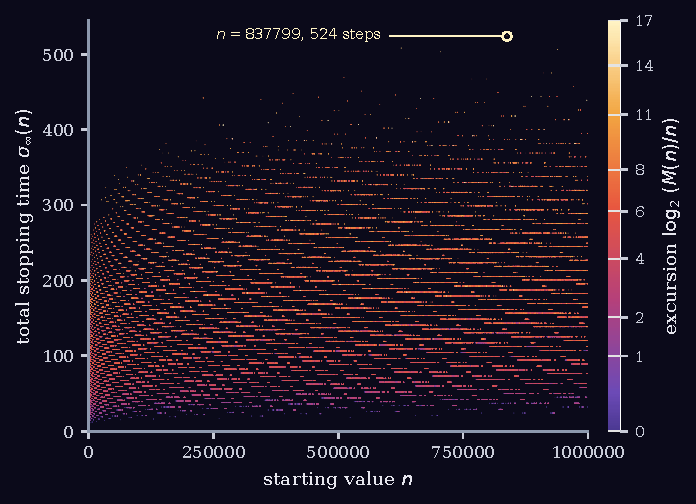
\includegraphics[width=\textwidth,height=0.78\textheight,keepaspectratio]{figures/art_g_stopping}
\caption{The total stopping time landscape. Each of the integers $2\le n\le10^6$ is
one point at height $\sigma_\infty(n)$, coloured by the excursion
$\log_2(M(n)/n)$; the longest orbit belongs to $n=837799$, with $524$ steps, and
the largest excursion to $n=159487$, which climbs to $M(n)=17\,202\,377\,752$,
a factor of about $2^{16.7}$. The horizontal streaks are runs of consecutive
integers whose orbits merge after a few steps, and the slow upward drift of the
cloud is the logarithmic growth of total stopping times discussed in
\cref{chap:intro} and \cref{chap:stochastic}.}
\label{fig:gal:stopping}
\end{figure}

\begin{figure}[p]
\centering
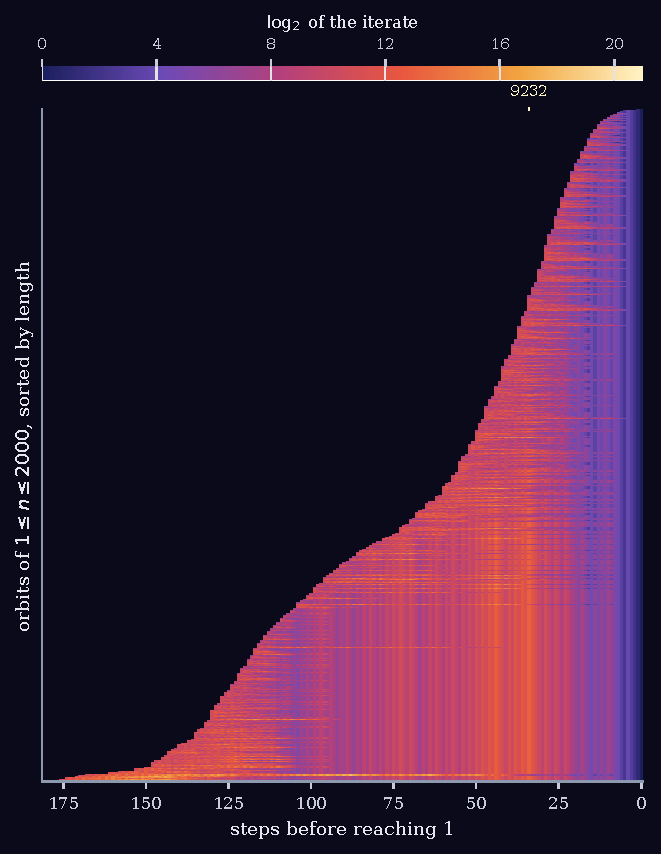
\includegraphics[width=\textwidth,height=0.78\textheight,keepaspectratio]{figures/art_g_heatmap}
\caption{The orbits of $1\le n\le2000$, one per row, written from right to left
so that every orbit ends at $1$ in the last column; colour is $\log_2$ of the
iterate, and the rows are sorted by orbit length, so the left edge is the
sorted list of total stopping times, rising to $181$ steps for $n=1161$. The bright
vertical band $34$ steps from the end is the value $9232$, through which $772$
of the $2000$ orbits pass: shared tails line up as columns, which is the
inverse tree of the next plate seen edge on.}
\label{fig:gal:heatmap}
\end{figure}

\begin{figure}[p]
\centering
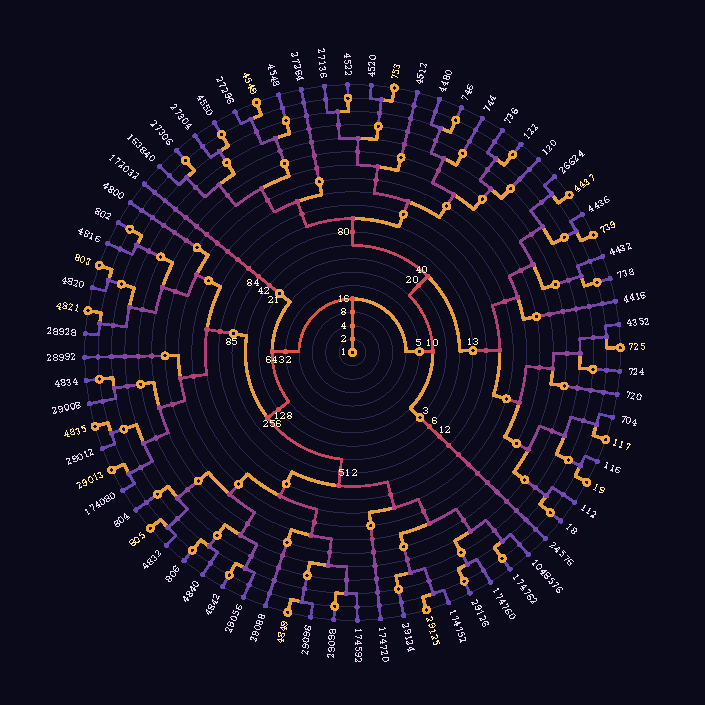
\includegraphics[width=\textwidth,height=0.78\textheight,keepaspectratio]{figures/art_g_tree}
\caption{The inverse tree of $1$ to depth $20$. The children of $m$ are $2m$ and, when $m\equiv4\pmod6$ and $m>4$, the odd number $(m-1)/3$; radius is depth, so the ring at radius $d$ holds exactly the $n$ with $\sigma_\infty(n)=d$. The tree has $342$ nodes; its $72$ leaves, the numbers with total stopping time $20$, run from $18$ to $2^{20}=1048576$, and the open circles mark the odd children, the only places where the tree branches; the branching random walk model of this tree, due to Lagarias and Weiss~\cite{lagarias1992}, is mentioned in \cref{chap:stochastic}.}
\label{fig:gal:tree}\index{Lagarias, J. C.}\index{Weiss, A.}
\end{figure}

\begin{figure}[p]
\centering
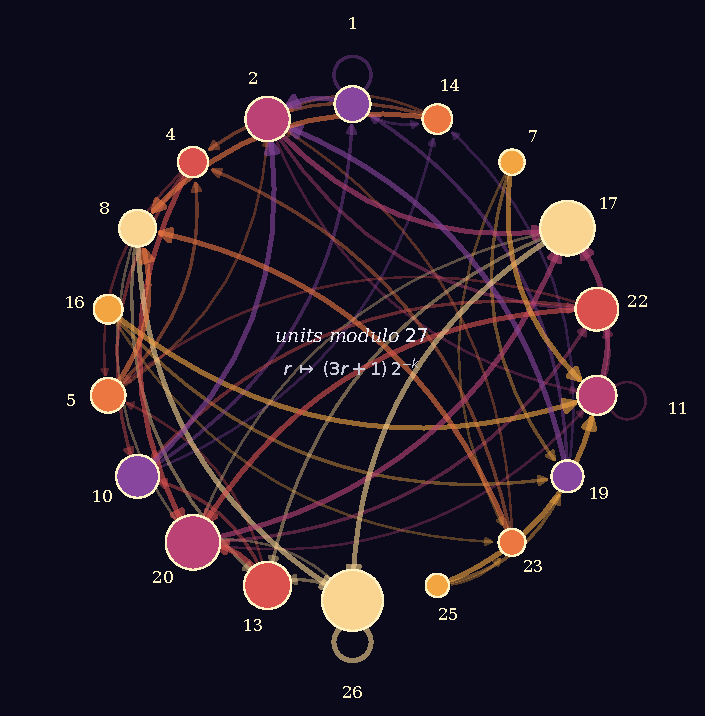
\includegraphics[width=0.94\textwidth,height=0.78\textheight,keepaspectratio]{figures/art_g_mod27}
\caption{The model chain on the $18$ units modulo $27$, in which the halving exponents are independent Geometric$(\tfrac12)$ draws: $r$ moves to $(3r+1)2^{-k}$ with probability $2^{-k}$, which for one stride from a uniformly random odd $y\equiv r$ holds exactly in the limit (\cref{chap:divergence}); with the units placed in the order $2^0,2^1,\ldots,2^{17}$, division by $2$ is one step clockwise, so the out edges of $r$ fan clockwise from $3r+1$. Edges with $k\le3$ are shown, and the three units $r$, $r+9$, $r+18$ share a shade because their common residue modulo $9$ alone determines the out edges; node area is the exact stationary law, largest at $26$ ($46570/262143\approx0.18$, with a loop of probability about $\tfrac12$) and smallest at $25$ ($1598/262143\approx0.006$), and it projects onto the law $\tfrac1{63}(8,16,11,4,2,22)$ modulo $9$.}
\label{fig:gal:mod27}
\end{figure}

\begin{figure}[p]
\centering
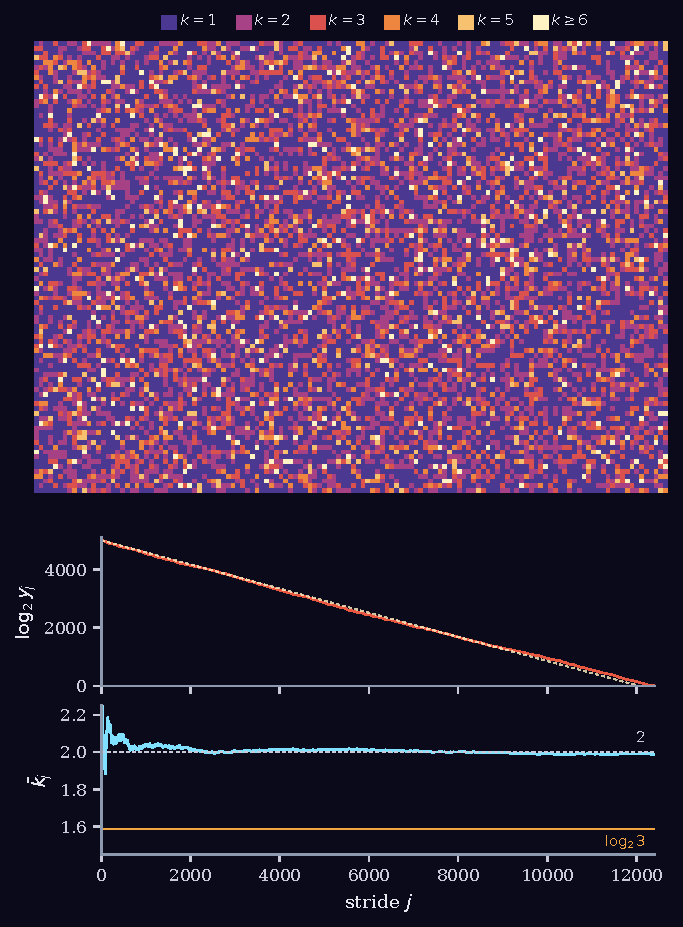
\includegraphics[width=0.9\textwidth,height=0.78\textheight,keepaspectratio]{figures/art_g_giant}
\caption{A giant orbit. Starting from $x_0=3^{3155}\approx2^{5000.56}$, the
Syracuse map takes $12408$ strides ($37075$ steps of $T_0$) to reach $1$. The
mosaic shows the exponents $k_j=\vt(3y_{j-1}+1)$ in reading order, $132$ to a
row, with frequencies $0.504$, $0.249$ and $0.128$ for $k=1,2,3$, close to the
Geometric law of \cref{chap:parity}; the descent of $\log_2y_j$
follows the drift line of slope $\log_23-2$ per stride (dashed), and the running mean
$\bar k_j$ settles near $2$, ending at $1.98799$; it lies at or below the
threshold $\log_23$ of \cref{chap:divergence} only for $j\le10$.}
\label{fig:gal:giant}
\end{figure}

\begin{figure}[p]
\centering
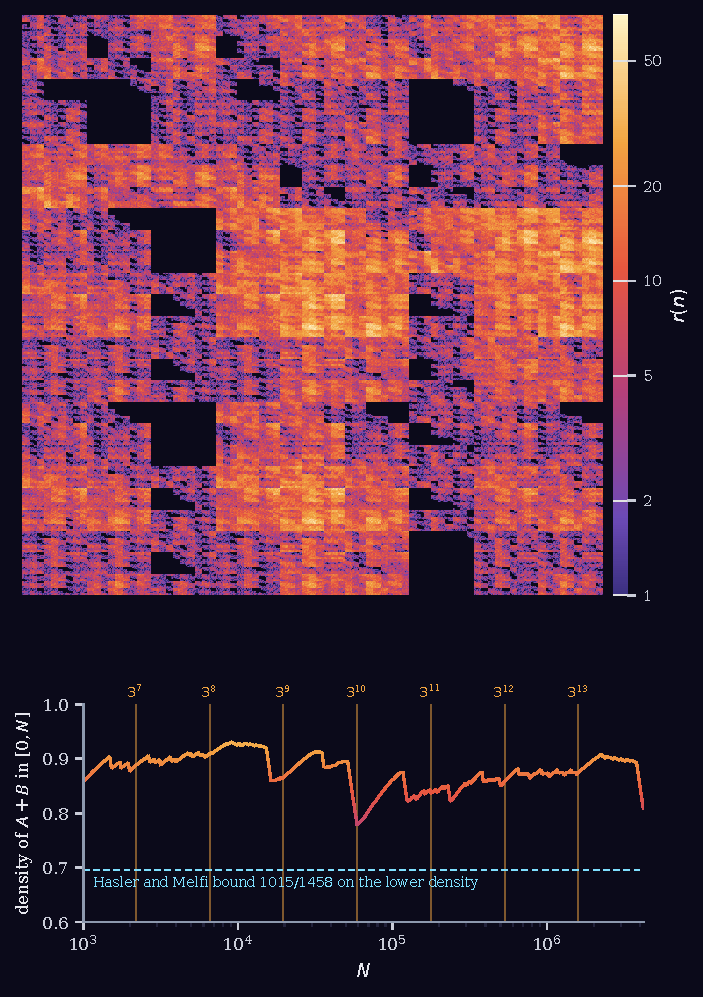
\includegraphics[width=0.9\textwidth,height=0.77\textheight,keepaspectratio]{figures/art_g_erdos}
\caption{The Erd\H{o}s $125$ sumset of \cref{chap:cycles}, with $A$ the numbers
whose base $3$ digits are $0$ or $1$ and $B$ the same in base $4$. Top: the
number $r(n)$ of representations $n=a+b$ for $n<3^{12}$, placed on a
$729\times729$ square with column and row read from the even and odd position
base $3$ digits of $n$; dark holes are gaps of $A+B$, which covers $85.83$
percent of this range, and $r(n)$ reaches $70$. Bottom: the density of $A+B$ in
$[0,N]$ for $10^3\le N\le4^{11}$, whose lowest value, $0.7785$, occurs at
$N=3^{10}-1$, well above $1015/1458\approx0.696$, the upper bound of Hasler and Melfi~\cite{haslermelfi2024} on the lower density.}
\label{fig:gal:erdos}\index{Hasler, M. F.}\index{Melfi, G.}
\end{figure}

\begin{figure}[p]
\centering
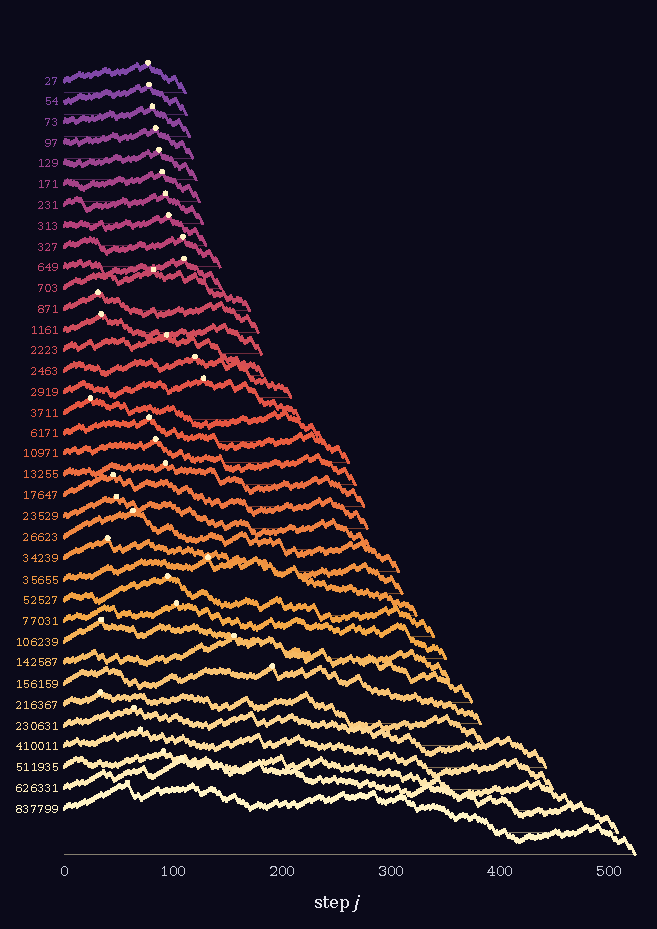
\includegraphics[width=0.92\textwidth,height=0.78\textheight,keepaspectratio]{figures/art_g_ridges}
\caption{Ridgelines of the total stopping time records. Up to $10^6$ there are $44$
integers whose total stopping time exceeds that of every smaller integer; for the
$36$ of them from $27$ ($111$ steps) to $837799$ ($524$ steps) each ridge traces
$\log_2T_0^{(j)}(n)$ until the orbit reaches $1$, with a pale dot at its
maximum. The highest summit belongs to $626331$, which climbs to
$7\,222\,283\,188$; the saw teeth are the alternation of rises by about
$\log_23$ and falls by $1$ whose net balance is the
descent problem of \cref{chap:lyapunov}.}
\label{fig:gal:ridges}
\end{figure}

\clearpage
\setcounter{figure}{\galsavedfigure}
\endgroup


\renewcommand{\partimagehook}{}
\appendix
\crefalias{chapter}{appendix}
\chapter{Numerical Constants}\label{app:constants}

\Cref{tab:appA:constants} collects the main constants used in the book, to
six significant figures unless stated otherwise. All were recomputed for this
book with the scripts of \cref{app:code}.

\begin{table}[ht]
\centering\small\setlength{\tabcolsep}{4pt}
\caption{Numerical constants.}
\label{tab:appA:constants}
\begin{tabular}{@{}lrl@{}}
\toprule
Constant & Value & Meaning \\
\midrule
$\log 2$ & $0.693147$ & one halving \\
$\log(3/2)$ & $0.405465$ & asymptotic odd step of $T$ \\
$\log(3/4)$ & $-0.287682$ & drift per stride of $S$, model \\
$\tfrac13\log(3/4)$ & $-0.0958940$ & drift per step of $T_0$, model \\
$\ds=\log(\sqrt3/2)$ & $-0.143841$ & drift per step of $T$ \\
$\sigma^2$ & $0.301737$ & step variance of $T$ \\
$2(\log2)^2$ & $0.960906$ & stride variance of $S$, model \\
$\E[\Delta^2]$ & $1.04367$ & second moment of a stride, model \\
$\tfrac2{27}(\log6)^2$ & $0.237808$ & long run step variance of $T_0$, model \\
$1/|\ds|$ & $6.95212$ & total stopping time slope, $T$, model \\
 & $6.91960$ & the same, observed for $n\le10^4$ \\
$\sigma^2/|\ds|^3$ & $101.387$ & variance slope, $T$, model \\
$3/|\log(3/4)|$ & $10.4282$ & total stopping time slope, $T_0$, model \\
$1/|\log(3/4)|$ & $3.47606$ & total stopping time slope, $S$, model \\
$C=\sigma^2/(\ds)^{2}$ & $14.5836$ & central limit constant \\
$D$ & $0.0346882$ & Chernoff rate, density theorem \\
$e^{-D}$ & $0.965907$ & Chernoff factor per step \\
$1/\log_23$ & $0.630930$ & critical frequency of odd steps, $T$ \\
$H(1/\log_23)$ in bits & $0.949956$ & residue sieve exponent $h$ \\
$\log_2 3$ & $1.58496$ & Ces\`aro threshold \\
$\beta=\log_23-1$ & $0.584963$ & Switching MM momentum \\
$L=\log(5/3)$ & $0.510826$ & largest stride ascent \\
$\log(10/3)$ & $1.20397$ & largest step ascent of $T_0$ \\
$\kappa=L/|\log(3/4)|$ & $1.77566$ & stride ratio (an analogy) \\
$\kappa_*=\log2/|\log(3/4)|$ & $2.40942$ & per step ratio (an analogy) \\
$\log(10/3)/|\log(3/4)|$ & $4.18508$ & step ratio of $T_0$ (an analogy) \\
$\rho(h)$ & $(-\tfrac12)^h$ & parity autocorrelation, model \\
$\mathcal A$ & $1/3$ & long run variance factor \\
$(2+2\beta+\beta^2)/(2+\beta)$ & $1.35867$ & SMM noise amplification \\
$1/(1-\beta)$ & $2.40942$ & every step amplification \\
$(2+\beta)/2$ & $1.29248$ & SMM effective step multiplier \\
$(2+\beta)/(1+\beta)$ & $1.63093$ & SMM stability limit for $\alpha\lambda$ \\
$\theta^*$ & $1$ & Wald root, accelerated model \\
\bottomrule
\end{tabular}
\end{table}

\section*{The continued fraction of $\log_23$}

To the precision of our computations ($300$ digits, with the first $60$ partial quotients confirmed at $150$),
\begin{multline*}
  \log_23=[1;1,1,2,2,3,1,5,2,23,2,2,1,1,\\
  55,1,4,3,1,1,15,1,9,2,5,\dots].
\end{multline*}
The large partial quotients $23$ and $55$ make the convergents just before
them, $p_8/q_8=\tfrac{1054}{665}$ and $p_{13}/q_{13}=\tfrac{301994}{190537}$, exceptionally good
two sided approximations. Only the second lies above $\log_23$ and counts for the one sided cycle bound of \cref{chap:cycles}, which jumps from $r=190\,537$ to the next rung of the ladder, $r=10\,781\,274$; the first lies below, with $\lceil665\log_23\rceil-665\log_23=0.99994$, and is useless there (\cref{rem:ch8:false}). With the verified range
$X=2^{n}$, the exact lower bounds on the number of odd elements $r$ and
halvings $s$ of a nontrivial cycle are given in \cref{tab:appA:cycles}.
The established range is $X=2^{71}$, by Ba\v{r}ina\index{Barina, D.@Ba\v{r}ina, D.}~\cite{barina2025}, and there the bound is the same as at $2^{68}$. The last row is nevertheless the current record, $r\ge137\,528\,045\,312$~\cite[\S6]{barina2025}: Hercher\index{Hercher, C.}'s sharper accounting of the cycle~\cite[Corollary~29]{hercher2023} reaches it already from $X=3\cdot2^{69}<2^{71}$.

\begin{table}[ht]
\centering\small
\caption{Exact cycle bounds from the ladder of $\log_23$, as functions of the
verified range $X$. Only $X\le2^{71}$ is established; the last row shows
what a larger range would give by this method.}
\label{tab:appA:cycles}
\begin{tabular}{@{}rrr@{}}
\toprule
$X$ & $r\ge$ & $s\ge$ \\
\midrule
$2^{40}$ & $10\,781\,274$ & $17\,087\,915$ \\
$2^{60}$ & $397\,573\,379$ & $630\,138\,897$ \\
$2^{68}$ & $72\,057\,431\,991$ & $114\,208\,327\,604$ \\
$2^{71}$ & $72\,057\,431\,991$ & $114\,208\,327\,604$ \\
$2^{72}$ & $137\,528\,045\,312$ & $217\,976\,794\,617$ \\
\bottomrule
\end{tabular}
\end{table}

\chapter{Code}\label{app:code}

Every number computed in this book was produced by a short Python script; numbers quoted from the literature are cited where they appear.
The scripts use the standard scientific stack (mpmath, NumPy, SciPy, SymPy and Matplotlib), with Numba for the census of \cref{sec:ch3:missing} and for the gallery, CVXPY with the Clarabel solver for the performance estimation of \cref{chap:difference}, and scikit-learn only to load the data set of \cref{sec:ch7:experiments}; they run in seconds to minutes on a laptop.
They are in the folder \texttt{book/scripts} of the book's repository, \url{https://github.com/VadimSokolov/collatz}, and are released under the MIT License.
The two Lean files of \cref{sec:ch8:lean} are in its folder \texttt{lean}.
This appendix lists two of them in full and indexes the rest.

\section{The exact cycle bound}

The script below computes the partial quotients of $\log_23$ at eighty digits,
builds the candidate rungs $q_{k-1}+jq_k$, keeps those that are records of the
one sided distance $\delta(r)=\lceil r\log_23\rceil-r\log_23$, and returns the
first rung not excluded by a verified range $X$.
By \cref{thm:ch8:onesided} and the mediant lemma (\cref{lem:ch8:mediant}) this is the exact bound.
Its output reproduces Eliahou's\index{Eliahou, S.} bound $s\ge17\,087\,915$~\cite{eliahou1993} at $X=2^{40}$ (with $r\ge10\,781\,274$) and gives $r\ge72\,057\,431\,991$ at $X=2^{68}$, unchanged at the current range $X=2^{71}$~\cite{barina2025}.

\begin{lstlisting}
# Exact lower bound on the number r of odd elements
# of a nontrivial Syracuse cycle, given that every
# n <= X reaches 1.  By the mediant lemma only rungs
# of the one sided ladder of theta = log_2 3 need
# to be checked.
from mpmath import mp, mpf, log, ceil, floor
mp.dps = 80
theta = log(3) / log(2)

def partial_quotients(x, n=40):
    a = []
    for _ in range(n):
        ai = int(floor(x)); a.append(ai)
        x = 1 / (x - ai)
    return a

a = partial_quotients(theta)
q = [0, 1]                  # q_{-1} = 0, q_0 = 1
for ai in a[1:]:
    q.append(ai * q[-1] + q[-2])

# candidate rungs q_{k-1} + j q_k,
# then keep the records of delta
cands = sorted({q[k-1] + j * q[k]
                for k in range(1, len(q) - 1)
                for j in range(a[k] + 1)} - {0})
delta = lambda r: ceil(r * theta) - r * theta
rungs, best = [], mpf(2)
for r in cands:
    d = delta(r)
    if d < best:
        best = d; rungs.append((r, d))

def first_not_excluded(X):
    eps = 1 / (3 * X * log(2))
    return next(r for r, d in rungs if d < r * eps)

for e in (40, 60, 68, 71, 72):
    r = first_not_excluded(mpf(2) ** e)
    s = int(ceil(r * theta))
    print(f"X = 2^{e}:  r >= {r},  s >= {s}")
\end{lstlisting}

\section{The noise amplification of Switching MM}

The second script derives the slow mode amplification factor of
\cref{thm:smmvar} symbolically. On one eigendirection with $a=\alpha\lambda$,
two steps of \smmdet\ starting from an even index contract the error by
$\rho=(1-a)(1-(1+\beta)a)$ and add noise of variance
$\alpha^2\sigma^2[(1-a)^2(1+\beta)^2+1]$.

\begin{lstlisting}
# Exact stationary variance of Switching MM on one
# eigendirection of a quadratic, a = alpha * lambda,
# unit noise (alpha^2 sigma^2 = 1).
import sympy as sp
a, b = sp.symbols('a b', positive=True)
# two step contraction and two step noise variance
rho = (1 - a) * (1 - (1 + b) * a)
q = (1 - a)**2 * (1 + b)**2 + 1
v_even = q / (1 - rho**2)
# odd phase: one descent step after an even time
v_odd = (1 - a)**2 * v_even + 1
v_avg = sp.simplify((v_even + v_odd) / 2)
# gradient descent gives 1/2
slow = sp.simplify(sp.limit(a * v_avg, a, 0))
print("slow mode a*Var:", slow)
V = sp.simplify(2 * slow)
print("amplification vs GD:", V)
print("at beta = log2(3) - 1:",
      float(V.subs(b, sp.log(3, 2) - 1)))
print("limit beta -> 1:", V.subs(b, 1))
\end{lstlisting}

\noindent Its output is the factor $((1+\beta)^2+1)/(2+\beta)$, equal to $1.3587$
at $\beta=\log_23-1$ and to $5/3$ in the limit $\beta\to1$.

\section{Index of scripts}

The scripts are grouped by the chapter that uses them, in the order of the book, and a script that reads the output of another is listed after it.
In particular \texttt{ch3\_o4\_decomp.py} writes the table of total stopping times of $T$ below $2^{26}$ that \texttt{ch3\_o4\_end.py} and most scripts of \cref{chap:samplers} read.

{\small
\begin{longtable}{@{}l>{\raggedright\arraybackslash}p{0.53\textwidth}@{}}
\toprule
Script & Purpose \\
\midrule
\endhead
\bottomrule
\endfoot
\multicolumn{2}{@{}l}{\itshape\Cref{chap:intro}} \\*
\texttt{ch01\_ch02\_figures.py} & orbit of $27$, total stopping times, residue tree of \cref{chap:parity} \\
\texttt{ch01\_ch02\_numbers.py} & worked orbits and delay records \\
\texttt{ch1\_slopes.py} & least squares slopes of the total stopping time against $\log n$ for $T_0$ and $T$, over $n\le10^4$ and $n\le10^5$ (\cref{sec:ch1:orbits}) \\
\addlinespace[4pt]
\multicolumn{2}{@{}l}{\itshape\Cref{chap:parity}} \\*
\texttt{ch02\_stopping.py} & Terras bijection, Chernoff bound \\
\texttt{ch02\_exact.py} & exact stopping counts by dynamic programming \\
\texttt{ch02\_extra.py} & orbit of $27$ by strides, $c_{70}(27)$, means over odd $n<2^{20}$, values of $\tau$ \\
\texttt{ch02\_checks.py} & Geometric counts below $2^{20}$, parity words of $T_0$ \\
\texttt{ch02\_figures.py} & Syracuse increment, sunburst, stopping heat map, $2$ adic shift \\
\texttt{ch2\_stopdecay.py} & decay of $1-F(k)$, binomial tail and Chernoff bound (\cref{fig:ch2:stopdecay}) \\
\addlinespace[4pt]
\multicolumn{2}{@{}l}{\itshape\Cref{chap:stochastic}} \\*
\texttt{ch3\_stats.py} & Lyapunov parameters, total stopping time CLT, parity autocorrelations, excursion tail \\
\texttt{ch3\_stopping.py} & total stopping time slope and standardized histogram \\
\texttt{ch3\_figures.py} & model paths, autocorrelations, Ville bound \\
\texttt{ch3\_o4\_model.py} & exact law of the model passage time \\
\texttt{ch3\_model\_means.py} & exact mean and variance of the model passage time \\
\texttt{ch3\_o4\_decomp.py} & exact census to $2^{30}$, variance decomposition \\
\texttt{ch3\_o4\_census.py} & exact census of total stopping times to $2^{30}$, skewness \\
\texttt{ch3\_o4\_end.py} & where the variance deficit lives \\
\addlinespace[4pt]
\multicolumn{2}{@{}l}{\itshape\Cref{chap:lyapunov}} \\*
\texttt{ch4\_ch5\_numbers.py} & two stride scans and other numbers of \cref{chap:lyapunov,chap:momentum}, crossings of the optimal coefficient \\
\texttt{ch4\_exact.py} & multi stride ascent densities, passage time of the stride model \\
\texttt{ch4\_figures.py} & strides, chained ascents \\
\addlinespace[4pt]
\multicolumn{2}{@{}l}{\itshape\Cref{chap:momentum}} \\*
\texttt{ch5\_numbers.py} & stride constants and their sensitivity, orbit of $27$ \\
\texttt{ch5\_parrondo.py} & capital dependent Parrondo games \\
\texttt{ch5\_nag\_check.py} & optimal constant momentum on quadratics, numerical check \\
\texttt{ch5\_figure.py} & optimal Nesterov coefficient against $\kappa$ (\cref{fig:ch5:nesterov}) \\
\addlinespace[4pt]
\multicolumn{2}{@{}l}{\itshape\Cref{chap:mmcollatz}} \\*
\texttt{ch5c\_mm.py} & residue potentials, positive cycles of $G_5$, block maps, run length potentials \\
\texttt{ch5c\_figures.py} & residue graph, block descent and run length potential (\cref{fig:ch5c:residue,fig:ch5c:runpot}) \\
\addlinespace[4pt]
\multicolumn{2}{@{}l}{\itshape\Cref{chap:smm}} \\*
\texttt{smm\_rate.py} & rate algebra of Switching MM \\
\texttt{ch6\_checks.py} & two step identity, defect, period two Chebyshev schedule \\
\texttt{ch6\_contraction.py} & per step contraction factors and their crossings (\cref{fig:ch6:contraction}) \\
\texttt{ch6\_trajectory.py} & two dimensional trajectories (\cref{fig:ch6:traj}) \\
\texttt{ch6\_ablation.py} & frequency ablation run to convergence \\
\addlinespace[4pt]
\multicolumn{2}{@{}l}{\itshape\Cref{chap:noise}} \\*
\texttt{smm\_variance\_book.py} & the second listing above \\
\texttt{smm\_var.py} & symbolic and numerical stationary variances of SMM, NAG and HB \\
\texttt{smm\_sim.py} & simulated slow mode variance against the leading term \\
\texttt{ch7\_variance.py} & exact stationary variances, amplification figure, predicted noise ratios \\
\texttt{ch7\_gainweight.py} & gain weight theorem, periodic Lyapunov checks \\
\texttt{ch7\_gainweight\_fig.py} & gain weight figure (\cref{fig:ch7:gainweight}) \\
\texttt{ch7\_pareto.py} & period two rate and noise frontier \\
\texttt{ch7\_multiplicative.py} & curvature noise, stability thresholds \\
\texttt{ch7\_experiments.py} & sweep, ablation, noise, logistic and minibatch runs \\
\texttt{ch7\_experiments\_fig.py} & figures of the sweep, the ablation, the logistic runs and the minibatch runs \\
\texttt{ch7\_noisefig.py} & noise experiment against theory (\cref{fig:ch7:noise}) \\
\texttt{ch7\_reconcile.py} & observed and predicted noise ratios \\
\texttt{ch7\_extra.py} & closed forms, bounds, logistic predictions \\
\addlinespace[4pt]
\multicolumn{2}{@{}l}{\itshape\Cref{chap:difference}} \\*
\texttt{ch5b\_tree.py} & certified exponents for the inverse tree \\
\texttt{ch5b\_tree\_exact.py} & the same certificates checked in exact integer arithmetic \\
\texttt{ch5b\_counts.py} & exact counting functions on the tree \\
\texttt{ch5b\_chains.py} & large scale growth of the doubling chain construction \\
\texttt{ch5b\_jsr.py} & exact joint spectral radius \\
\texttt{ch5b\_pep.py} & performance estimation for two steps \\
\texttt{ch5b\_transient.py} & transient grid behind the transient bound conjecture \\
\texttt{ch5b\_figures.py} & figures of the chapter \\
\addlinespace[4pt]
\multicolumn{2}{@{}l}{\itshape\Cref{chap:threepoint}} \\*
\texttt{ch5d\_pep.py} & convex performance estimation for six methods \\
\texttt{ch5d\_golden.py} & the exact rate of Switching MM across $\beta$ \\
\texttt{ch5d\_threshold.py} & the thresholds $\beta_N$ \\
\texttt{ch5d\_cross.py} & switched triangles against Switching MM \\
\texttt{ch5d\_collatz\_bregman.py} & Bregman decomposition and dissipation \\
\texttt{ch5d\_figures.py} & figures of the chapter \\
\addlinespace[4pt]
\multicolumn{2}{@{}l}{\itshape\Cref{chap:cycles}} \\*
\texttt{cycle\_bound\_book.py} & the first listing above \\
\texttt{ch08\_negative.py} & cycles on the negative integers \\
\texttt{ch08\_compute.py} & continued fraction at $300$ digits, confirmed at $150$, and the convergents \\
\texttt{ladder.py} & ladder rungs, exact and crude bounds \\
\texttt{ch08\_records.py} & records of $r/(3\Lambda_r)$ in exact arithmetic, against the ladder \\
\texttt{ch08\_bounds.py} & block bounds $B_k$ and the sharp bound at $150$ digits \\
\texttt{ch08\_ties.py} & ties in double and $150$ digit arithmetic, exact record scan \\
\texttt{ch08\_crude.py} & exact versus crude bound \\
\texttt{ch08\_figures.py} & figures of the records and the one sided distances \\
\texttt{ch08\_profile.py} & thresholds, insufficiency, irrationality profile \\
\texttt{ch08\_window.py} & window lemma and parity word exploration \\
\texttt{ch08\_certificate.py} & exact integer certificate at $2^{68}$ \\
\texttt{ch08\_erdos125.py} & density of the Erd\H{o}s $125$ sumset \\
\texttt{ch08\_erdos125\_fig.py} & figure of the Erd\H{o}s $125$ density \\
\texttt{ch08\_misc.py} & small checks: the longest orbit of $T$ up to $10^4$, the rational cycle of $\tfrac15$ \\
\addlinespace[4pt]
\multicolumn{2}{@{}l}{\itshape\Cref{chap:divergence}} \\*
\texttt{ch9\_cesaro\_scan.py} & terminal $\bar k_N$ for odd $3\le x_0\le5001$ (\cref{rem:ch9:circular}) \\
\texttt{ch9\_figures.py} & running $\bar k_N$ and the Syracuse law modulo $9$ (\cref{fig:ch9:kbar,fig:ch9:syrlaw}) \\
\texttt{ch9\_numbers.py} & the Ces\`aro identity along three long orbits, odd step thresholds \\
\texttt{ch9\_spectral.py} & model chains modulo $3^a$, empirical transitions \\
\texttt{ch9\_table.py} & restricted and full transition matrices modulo $3^a$ (\cref{tab:ch9:moduli}) \\
\texttt{ch9\_orbits.py} & residues along single orbits from $2^{10000}$ \\
\texttt{ch9\_orbits\_check.py} & single orbits against the model chain, chi squared checks \\
\addlinespace[4pt]
\multicolumn{2}{@{}l}{\itshape\Cref{chap:backward}} \\*
\texttt{ch9b\_steps.py} & steps of $T_0$ and $S$ for $n<3\cdot10^6$ against Lau's bounds (\cref{tab:ch9b:steps}) \\
\texttt{ch9b\_tree.py} & the backward tree from $1$ below $2^{24}$, exactly (\cref{tab:ch9b:tree}) \\
\texttt{ch9b\_offset\_law.py} & the exact $3$ adic offset law to level $18$, with a full Fourier transform at every level (\cref{tab:ch9b:offsets,tab:ch9b:profile}) \\
\texttt{ch9b\_figures.py} & renewal constants, \cref{fig:ch9b:steps,fig:ch9b:fourier,fig:ch9b:tree,fig:ch9b:crossing} \\
\addlinespace[4pt]
\multicolumn{2}{@{}l}{\itshape\Cref{chap:computation}} \\*
\texttt{ch10b\_sieve.py} & residue sieve counts and entropy exponent \\
\texttt{ch10b\_divsieve.py} & divisibility sieve for cycles \\
\texttt{ch10b\_figures.py} & residue sieve counts and the uncovered classes in the $2$ adic coordinate (\cref{fig:ch10b:sieve}) \\
\addlinespace[4pt]
\multicolumn{2}{@{}l}{\itshape\Cref{chap:samplers}} \\*
\texttt{ch10b\_nested.py} & exact partition function, nested sampling runs, evidence at $\beta=0.02$ \\
\texttt{ch10b\_nested2.py} & decay of the level set volumes, nested search for the slowest integers \\
\texttt{ch10c\_perfect.py} & perfect split sampling for the coefficient stopping time \\
\texttt{ch10c\_ladder.py} & exact staircase, hazards, fits, partition function at $\beta=D$ \\
\texttt{ch10c\_montecarlo.py} & nested, split and vertical likelihood samplers \\
\texttt{ch10c\_acceptance.py} & bit flip acceptance inside level sets \\
\texttt{ch10c\_clusters.py} & coalescence classes of the level sets \\
\texttt{ch10c\_trees.py} & trees by box size and level \\
\texttt{ch10c\_treerecords.py} & trunks, tributaries and delay records \\
\texttt{ch10c\_treemodel.py} & naive model of tree sizes \\
\texttt{ch10c\_figures.py} & staircase, perfect sampler and sampler comparison (\cref{fig:ch10b:montecarlo}) \\
\texttt{ch10c\_acceptance\_fig.py} & acceptance and class sizes (\cref{fig:ch10b:acceptance}) \\
\addlinespace[4pt]
\multicolumn{2}{@{}l}{\itshape\Cref{chap:progress}} \\*
\texttt{ch16\_o4\_cumulants.py} & cumulant deficits and the split at $2^{14}$ \\
\texttt{ch16\_o4\_predict.py} & out of sample skewness to $2^{49}$ \\
\texttt{ch16\_pep\_dual.py} & dual multipliers of performance estimation \\
\texttt{ch16\_pep\_sparse.py} & sparse certificates \\
\texttt{ch16\_certificate.py} & closed form certificate, symbolic minors \\
\texttt{ch16\_fullconj.py} & the two branch conjecture \\
\texttt{ch16\_s2\_softmax.py} & noise floors on the digits problem \\
\texttt{ch16\_erdos125.py} & Erd\H{o}s $125$ to $4^{17}$ \\
\texttt{ch16\_p3\_orbits.py} & single orbits from $2^{300000}$ \\
\texttt{ch16\_figures.py} & figures of the chapter \\
\addlinespace[4pt]
\multicolumn{2}{@{}l}{\itshape\Cref{chap:synthesis}} \\*
\texttt{ch10d\_figures.py} & road map of the chapter \\
\addlinespace[4pt]
\multicolumn{2}{@{}l}{\itshape Utilities and the gallery} \\*
\texttt{bookstyle.py} & shared style of the figures \\*
\texttt{make\_index\_tags.py} & places index entries in the text \\*
\texttt{art\_*.py} & cover, part openers and gallery plates \\
\end{longtable}}


\backmatter
\bibliographystyle{plainnatto}
\bibliography{refs,refs_A,refs_B,refs_C,refs_D,refs_E,refs_F,refs_G}
\printindex

\end{document}
